% Template pour faire aide-mémoire
\documentclass[10pt, french]{article}
%% -----------------------------
%% Préambule
%% -----------------------------
% !TEX encoding = UTF-8 Unicode
% LaTeX Preamble for all cheatsheets
% Author : Gabriel Crépeault-Cauchon

% HOW-TO : copy-paste this file in the same directory as your .tex file, and add in your preamble the next command right after you have specified your documentclass : 
% \input{preamble-cheatsht.tex}
% ---------------------------------------------
% ---------------------------------------------

% Extra note : this preamble creates document that are meant to be used inside the multicols environment. See the documentation on internet for further information.

%% -----------------------------
%% Encoding packages
%% -----------------------------
\usepackage[utf8]{inputenc}
\usepackage[T1]{fontenc}
\usepackage{babel}
\usepackage{lmodern}
\usepackage[colorinlistoftodos]{todonotes}
%% -----------------------------
%% Variable definition
%% -----------------------------
\def\auteur{\href{https://github.com/ressources-act/Guide_de_survie_en_actuariat/blob/master/02_Cheatsheets/contributeurs/contributeurs-cheatshts.pdf}{\faGithub \ Liste des contributeurs}}
\def\BackgroundColor{white}
\usepackage{xargs} % for more logical new function creation

%% -----------------------------
%% Margin and layout
%% -----------------------------
% Determine the margin for cheatsheet
\usepackage[landscape, hmargin=1cm, vmargin=1.7cm]{geometry}
\usepackage{multicol}

% Remove automatic indentation after section/subsection title.
\setlength{\parindent}{0cm}

% Save space in cheatsheet by removing space between align environment and normal text.
\usepackage{etoolbox}
\newcommand{\zerodisplayskips}{%
  \setlength{\abovedisplayskip}{0pt}%
  \setlength{\belowdisplayskip}{0pt}%
  \setlength{\abovedisplayshortskip}{0pt}%
  \setlength{\belowdisplayshortskip}{0pt}}
\appto{\normalsize}{\zerodisplayskips}
\appto{\small}{\zerodisplayskips}
\appto{\footnotesize}{\zerodisplayskips}

%% -----------------------------
%% URL and links
%% -----------------------------
\usepackage{hyperref}
\hypersetup{colorlinks = true, urlcolor = gray!70!white, linkcolor = black}

%% -----------------------------
%% Document policy (uncomment only one)
%% -----------------------------
%	\usepackage{concrete}
	\usepackage{mathpazo}
%	\usepackage{frcursive} %% permet d'écrire en lettres attachées
%	\usepackage{aeguill}
%	\usepackage{mathptmx}
%	\usepackage{fourier} 

%% -----------------------------
%% Math configuration
%% -----------------------------
\usepackage[fleqn]{amsmath}
\usepackage{amsthm,amssymb,latexsym,amsfonts}
\usepackage{gensymb}
\usepackage{empheq}
\usepackage{numprint}
\usepackage{dsfont} % Pour avoir le symbole du domaine Z
%\usepackage{bigints} % pour des gros intégrales
% Mathematics shortcuts
\usepackage{scalerel,stackengine,amsmath}
\newcommand\equalhat{\mathrel{\stackon[1.5pt]{=}{\stretchto{%
    \scalerel*[\widthof{=}]{\wedge}{\rule{1ex}{3ex}}}{0.5ex}}}}
\newcommand{\reels}{\mathbb{R}}
\newcommand{\entiers}{\mathbb{Z}}
\newcommand{\naturels}{\mathbb{N}}
\newcommand{\eval}{\biggr \rvert}
\usepackage{cancel}
\newcommand{\derivee}[1]{\frac{\partial}{\partial #1}}
\newcommand{\prob}[1]{\Pr \left( #1 \right)}
\newcommand{\esp}[1]{\mathrm{E} \left[ #1 \right]} % espérance
\newcommand{\variance}[1]{\mathrm{Var} \left( #1   \right)}
\newcommand{\covar}[1]{\mathrm{Cov} \left( #1   \right)}
\newcommand{\laplace}{\mathcal{L}}
\newcommand{\deriv}[3][]{\frac{\partial^{#1}#3}{\partial #2^{#1}}}
\newcommand{\e}[1]{\mathrm{e}^{#1}}
\newcommand{\te}[1]{\text{exp}\left\{#1\right\}}
\DeclareMathSymbol{\shortminus}{\mathbin}{AMSa}{"39}
%%	Example usage:	\sumz{n}{i = 1} <=> \overset{n}{\underset{i = 1}{\sum}}
\newcommand{\sumz}[2]{\overset{#1}{\underset{#2}{\sum}}}
%%	Example usage:	\limz{h}{0} <=> \underset{h \rightarrow 0}{\lim}
\newcommand{\limz}[2]{\underset{#1 \rightarrow #2}{\lim}}
%%	Example usage:	\LVx{h}	<=>	\actsymb[h]{L}{}[]
%%					\LVx[n]{h}	<=>	\actsymb[h]{L}{}[n]
\newcommand{\LVx}[2][]{\actsymb[#2]{L}{}[#1]}
\DeclareMathOperator*{\argmax}{arg\,max}
\DeclareMathOperator*{\argmin}{arg\,min}
%%%	\icbox{<frame color>}{<background color>}{<text>}
\newcommandx{\icbox}[3][1 = bleudefrance, 2 = beaublue]{\fcolorbox{#1}{#2}{#3}}
%%	other good color combo is azure(colorwheel) arsenic
\usepackage{longfbox}
%	voir cette page, paquetage avec CSS https://ctan.math.illinois.edu/macros/latex/contrib/longfbox/longfbox.html
\newfboxstyle{rappel}{
	background-color = tealblue!20!white, 
	border-style = outset,
	breakable = true,
%	
	border-color = tealblue,
	border-radius = 1ex, 
%
	padding-bottom = 0.2ex,
	padding-top = 0.2ex,
	padding-left = 0.4ex,
	padding-right = 0.4ex,
%	
	border-top-width = 0.3ex,
	border-bottom-width = 0.3ex,
%
	border-left-width = 1ex, 
	border-bottom-left-radius = 0.2ex,
%	
	border-right-width = 1ex, 
	border-top-right-radius = 0.2ex,
%	
}
\newfboxstyle{formula}{ 
	background-color = beaublue, 
	border-color = bleudefrance
}
\newfboxstyle{imphl}{ 
	padding = 0pt,
	margin = 0pt,
	baseline-skip = false,
	background-color = palechestnut!60!white, 
	border-color = white
}
\newfboxstyle{conditions}{ 
	background-color = palechestnut, 
	border-color = red
}
\newcommandx{\rcbox}[3][1 = bleudefrance, 2 = beaublue]{\lfbox[border-radius = 0.5ex, background-color = #2, border-color = #1]{#3}}

% To indicate equation number on a specific line in align environment
\newcommand\numberthis{\addtocounter{equation}{1}\tag{\theequation}}

%
% Actuarial notation packages
%
\usepackage{actuarialsymbol}
\usepackage{actuarialangle}

%
% Matrix notation for math symbols (\bm{•})
%
\usepackage{bm}
% Matrix notation variable (bold style)
\newcommand{\matr}[1]{\mathbf{#1}}



%% -----------------------------
%% tcolorbox configuration
%% -----------------------------
\usepackage[most]{tcolorbox}
\tcbuselibrary{xparse}
\tcbuselibrary{breakable}

%%
%% Coloured box "definition" for definitions
%%
\DeclareTColorBox{definition}{ o }				% #1 parameter
{
	colframe=blue!60!green,colback=blue!5!white, % color of the box
	breakable, 
	pad at break* = 0mm, 						% to split the box
	title = {#1},
	after title = {\large \hfill \faBook},
}
%%
%% Coloured box "definition2" for definitions
%%
\DeclareTColorBox{definitionNOHFILL}{ o }				% #1 parameter
{
	colframe=blue!60!green,colback=blue!5!white, % color of the box
	pad at break* = 0mm, 						% to split the box
	title = {#1},
	before title = {\faBook \quad },
	breakable
}
%%
%% Coloured box "definition2" for definitions
%%
\DeclareTColorBox{definitionNOHFILLsub}{ o }				% #1 parameter
{
	colframe=blue!40!green,colback=blue!5!white, % color of the box
	pad at break* = 0mm, 						% to split the box
	title = {#1},
	before title = {\faNavicon \quad }, %faBars  faGetPocket
	breakable
}
%%
%% Coloured box "definition3" for propriétés
%%
\DeclareTColorBox{definitionNOHFILLprop}{ o }				% #1 parameter
{
	colframe=amber(sae/ece),colback=amber(sae/ece)!5!white, % color of the box
	pad at break* = 0mm, 						% to split the box
	title = {#1},
	before title = {\faGetPocket \quad }, %faBars  faGetPocket
	breakable
}
%%
%% Coloured box "definition3" for propriétés
%%
\DeclareTColorBox{definitionNOHFILLpropos}{ o }				% #1 parameter
{
	colframe=carmine,colback=carmine!5!white, % color of the box
	pad at break* = 0mm, 						% to split the box
	title = {#1},
	before title = {\faColumns \quad }, %\faEllipsisH  faColumns
	breakable
}


%%
%% Coloured box "algo" for algorithms
%%
\newtcolorbox{algo}[ 1 ]
{
	colback = blue!5!white,
	colframe = blue!75!black,
	title=#1,
	fonttitle = \bfseries,
	breakable
}
%%
%% Coloured box "conceptgen" for points adding to a concept's deifintion
%%
\newtcolorbox{conceptgen}[ 1 ]
{
	breakable,
	colback = beaublue,
	colframe = airforceblue,
	title=#1,
	fonttitle = \bfseries
}
%%
%% Coloured box "rappel" pour rappel de formules
%%
\DeclareTColorBox{conceptgen_enhanced}{ o }
{
	enhanced,
	title = #1,
	colback=beaublue, % color of the box
%	colframe=blue(pigment),
%	colframe=arsenic,	
	colbacktitle=airforceblue,
	fonttitle = \bfseries,
	breakable,
	boxed title style={size=small,colframe=arsenic} ,
	attach boxed title to top center = {yshift=-3mm,yshifttext=-1mm},
}
%%
%% Coloured box "probch3" pour formules relatives au 3ème chapitre de prob
%%
\newtcolorbox{probch3}[ 1 ]
{
	colback = ruddypink,
	colframe = burgundy,
	fonttitle = \bfseries,	
	breakable,
	title=#1
}
%%
%% Coloured box "formula" for formulas
%%
\newtcolorbox{formula}[ 1 ]
{
	colback = green!5!white,
	colframe = green!70!black,
	breakable,
	fonttitle = \bfseries,
	title=#1
}
%%
%% Coloured box "formula" for formulas
%%
\DeclareTColorBox{algo2}{ o }
{
	enhanced,
	title = #1,
	colback=blue!5!white,	
	colbacktitle=blue!75!black,
	fonttitle = \bfseries,
	breakable,
	boxed title style={size=small,colframe=arsenic} ,
	attach boxed title to top center = {yshift=-3mm,yshifttext=-1mm},
}
%%
%% Coloured box "examplebox" for formulas
%%
\newtcolorbox{examplebox}[ 1 ]
{
	colback = beaublue,
	colframe = amethyst,
	breakable,
	fonttitle = \bfseries,title=#1
}
%%
%% Coloured box "rappel" pour rappel de formules
%%
\newtcolorbox{rappel}[ 1 ]
{
	colback = ashgrey,
	colframe = arsenic,
	breakable,
	fonttitle = \bfseries,title=#1
}
%%
%% Coloured box "rappel" pour rappel de formules
%%
\DeclareTColorBox{rappel_enhanced}{ o }
{
	enhanced,
	title = #1,
	colback=ashgrey, % color of the box
%	colframe=blue(pigment),
%	colframe=arsenic,	
	colbacktitle=arsenic,
	fonttitle = \bfseries,
	breakable,
	boxed title style={size=small,colframe=arsenic} ,
	attach boxed title to top center = {yshift=-3mm,yshifttext=-1mm},
}
%%
%% Coloured box "notation" for notation and terminology
%%
\DeclareTColorBox{distributions}{ o }			% #1 parameter
{
	enhanced,
	title = #1,
	colback=gray(x11gray), % color of the box
%	colframe=blue(pigment),
	colframe=arsenic,	
	colbacktitle=aurometalsaurus,
	fonttitle = \bfseries,
	boxed title style={size=small,colframe=arsenic} ,
	attach boxed title to top center = {yshift=-3mm,yshifttext=-1mm},
	breakable
%	left=0pt,
%  	right=0pt,
%    box align=center,
%    ams align*
%  	top=-10pt
}
\newtcolorbox{contrib}[ 1 ]
{
	colback = babyblueeyes,
	colframe = airforceblue,
	fonttitle = \bfseries,
	title = {#1},
	valign = center
}

%% -----------------------------
%% Graphics and pictures
%% -----------------------------
\usepackage{graphicx}
\usepackage{pict2e}
\usepackage{tikz}

%% -----------------------------
%% insert pdf pages into document
%% -----------------------------
\usepackage{pdfpages}

%% -----------------------------
%% Color configuration
%% -----------------------------
\usepackage{color, soulutf8, colortbl}


%
%	Colour definitions
%
\definecolor{armygreen}{rgb}{0.29, 0.33, 0.13}	%	army
\definecolor{asparagus}{rgb}{0.53, 0.66, 0.42}	% pastel green militariesque
\definecolor{britishracinggreen}{rgb}{0.0, 0.26, 0.15}
\definecolor{calpolypomonagreen}{rgb}{0.12, 0.3, 0.17}
\definecolor{darkgreen}{rgb}{0.0, 0.2, 0.13}

\definecolor{antiquebrass}{rgb}{0.8, 0.58, 0.46}	% brown-ish light cardboard color

\definecolor{blue(munsell)}{rgb}{0.0, 0.5, 0.69}
\definecolor{blue(matcha)}{rgb}{0.596, 0.819, 1.00}
\definecolor{blue(munsell)-light}{rgb}{0.5, 0.8, 0.9}
\definecolor{bleudefrance}{rgb}{0.19, 0.55, 0.91}
\definecolor{blizzardblue}{rgb}{0.67, 0.9, 0.93}	%	mr.freeze light baby blue 
\definecolor{bondiblue}{rgb}{0.0, 0.58, 0.71}	%	darker cyan type inidgo blue
\definecolor{blue(pigment)}{rgb}{0.2, 0.2, 0.6}
\definecolor{bluebell}{rgb}{0.64, 0.64, 0.82}
\definecolor{airforceblue}{rgb}{0.36, 0.54, 0.66}
\definecolor{beaublue}{rgb}{0.74, 0.83, 0.9}    % almost white
\definecolor{blue_rectangle}{RGB}{83, 84, 244}		% ACT-2004
\definecolor{cobalt}{rgb}{0.0, 0.28, 0.67}	% nice light blue-ish
\definecolor{ballblue}{rgb}{0.13, 0.67, 0.8}	%	almost green ish blue ish
\definecolor{babyblueeyes}{rgb}{0.63, 0.79, 0.95}

\definecolor{indigo(web)}{rgb}{0.29, 0.0, 0.51}	% purple-ish
\definecolor{antiquefuchsia}{rgb}{0.57, 0.36, 0.51}	%	pastel matte (darkerish) purple ish
\definecolor{darkpastelpurple}{rgb}{0.59, 0.44, 0.84}	%	pretty purple
\definecolor{gray(x11gray)}{rgb}{0.75, 0.75, 0.75}
\definecolor{aurometalsaurus}{rgb}{0.43, 0.5, 0.5}
\definecolor{bulgarianrose}{rgb}{0.28, 0.02, 0.03}	%	dark maroon type 
\definecolor{pastelred}{rgb}{1.0, 0.41, 0.38}		%	light red pinktinybit ish
\definecolor{lightmauve}{rgb}{0.86, 0.82, 1.0}
\definecolor{eggshell}{rgb}{0.94, 0.92, 0.84}
\definecolor{azure(colorwheel)}{rgb}{0.0, 0.5, 1.0}
\definecolor{darkgreen}{rgb}{0.0, 0.2, 0.13}			
\definecolor{ao(english)}{rgb}{0.0, 0.5, 0.0}		% prertty apple dark pastel (light) green
\definecolor{green_rectangle}{RGB}{131, 176, 84}		% ACT-2004
\definecolor{red_rectangle}{RGB}{241,112,113}		% ACT-2004
\definecolor{amethyst}{rgb}{0.6, 0.4, 0.8}
\definecolor{amethyst-light}{rgb}{0.6, 0.4, 0.8}
\definecolor{ruddypink}{rgb}{0.88, 0.56, 0.59}

\definecolor{amber(sae/ece)}{rgb}{1.0, 0.49, 0.0} 	%	pretty orange ish
\definecolor{burntsienna}{rgb}{0.91, 0.45, 0.32}		%%	lighter pastel orange
\definecolor{burntorange}{rgb}{0.8, 0.33, 0.0}		%%	imilar but deeper orange
\definecolor{orange-red}{rgb}{1.0, 0.27, 0.0}

\definecolor{tealblue}{rgb}{0.21, 0.46, 0.53}

\definecolor{battleshipgrey}{rgb}{0.52, 0.52, 0.51}  % lilght ish gray
\definecolor{ashgrey}{rgb}{0.7, 0.75, 0.71}			% dark grey-black-ish
\definecolor{arsenic}{rgb}{0.23, 0.27, 0.29}			% light green-beige-ish gray
\definecolor{gray(x11gray)}{rgb}{0.75, 0.75, 0.75}

\definecolor{carmine}{rgb}{0.59, 0.0, 0.09} 			% deep red
\definecolor{amaranth}{rgb}{0.9, 0.17, 0.31}
\definecolor{brickred}{rgb}{0.8, 0.25, 0.33}
\definecolor{chestnut}{rgb}{0.8, 0.36, 0.36}		% pink red ish light
\definecolor{palechestnut}{rgb}{0.87, 0.68, 0.69}
\definecolor{pastelred}{rgb}{1.0, 0.41, 0.38}
\definecolor{forestgreen(traditional)}{rgb}{0.0, 0.27, 0.13}
%
% Useful shortcuts for coloured text
%
\newcommand{\orange}{\textcolor{orange}}
\newcommand{\red}{\textcolor{red}}
\newcommand{\cyan}{\textcolor{cyan}}
\newcommand{\blue}{\textcolor{blue}}
\newcommand{\green}{\textcolor{green}}
\newcommand{\purple}{\textcolor{magenta}}
\newcommand{\yellow}{\textcolor{yellow}}

%% -----------------------------
%% Enumerate environment configuration
%% -----------------------------
%
% Custum enumerate & itemize Package
%
\usepackage{enumitem}
%
% French Setup for itemize function
%
\frenchbsetup{StandardItemLabels=true}
%
% Change default label for itemize
%
\renewcommand{\labelitemi}{\faAngleRight}


%% -----------------------------
%% Tabular column type configuration
%% -----------------------------
\newcolumntype{C}{>{$}c<{$}} % math-mode version of "l" column type
\newcolumntype{L}{>{$}l<{$}} % math-mode version of "l" column type
\newcolumntype{R}{>{$}r<{$}} % math-mode version of "l" column type
\newcolumntype{f}{>{\columncolor{green!20!white}}p{1cm}}
\newcolumntype{g}{>{\columncolor{green!40!white}}m{1.2cm}}
\newcolumntype{a}{>{\columncolor{red!20!white}$}p{2cm}<{$}}	% ACT-2005
% configuration to force a line break within a single cell
\usepackage{makecell}


%% -----------------------------
%% Fontawesome for special symbols
%% -----------------------------
\usepackage{fontawesome}

%% -----------------------------
%% Section Font customization
%% -----------------------------
\usepackage{sectsty}
\sectionfont{\color{\SectionColor}}
\subsectionfont{\color{\SubSectionColor}}
\subsubsectionfont{\color{\SubSubSectionColor}}

%% -----------------------------
%% Footer/Header Customization
%% -----------------------------
\usepackage{lastpage}
\usepackage{fancyhdr}
\pagestyle{fancy}

%
% Header
%
\fancyhead{} 	% Reset
\fancyhead[L]{Aide-mémoire pour~\cours ~(\textbf{\sigle})}
\fancyhead[R]{\auteur}

%
% Footer
%
\fancyfoot{}		% Reset
\fancyfoot[R]{\thepage ~de~ \pageref{LastPage}}
\fancyfoot[L]{\href{https://github.com/ressources-act/Guide_de_survie_en_actuariat}{\faGithub \ ressources-act/Guide de survie en actuariat}}
%
% Page background color
%
\pagecolor{\BackgroundColor}




%% END OF PREAMBLE
% ---------------------------------------------
% ---------------------------------------------
%% -----------------------------
%% Variable definition
%% -----------------------------
\def\cours{Modern Actuarial Statistics I}
\def\sigle{MAS-I}
%
% 	Save more space than default
%
\setlength{\abovedisplayskip}{-15pt}
\setlist{leftmargin=*}
%
%	Extra math symbols
%

\usepackage{mathrsfs}
%
% 	thin space, limits underneath in displays

%% -----------------------------
%% 	Colour setup for sections
%% -----------------------------
\def\SectionColor{cobalt}
\def\SubSectionColor{azure(colorwheel)}
\def\SubSubSectionColor{azure(colorwheel)}
%%%	depth
\setcounter{secnumdepth}{0}
%% -----------------------------

%% -----------------------------
%% Color definitions
%% -----------------------------
\definecolor{indigo(web)}{rgb}{0.29, 0.0, 0.51}
\definecolor{cobalt}{rgb}{0.0, 0.28, 0.67}
\definecolor{azure(colorwheel)}{rgb}{0.0, 0.5, 1.0}
%% -----------------------------
%% Variable definition
%% -----------------------------
%%
%% Matrix notation variable (bold style)
%%
\newcommand\cololine[2]{\colorlet{temp}{.}\color{#1}\bar{\color{temp}#2}\color{temp}}
\newcommand\colbar[2]{\colorlet{temp}{.}\color{#1}\bar{\color{temp}#2}\color{temp}}
\newcommand\cumlaut[2][black]{\stackon[.33ex]{#2}{\textcolor{#1}{\kern-.04ex.\kern-.2ex.}}}

\begin{document}

\begin{center}
	\textsc{\Large Contributeurs}\\[0.5cm] 
%	\hl{Pendant mon étude de MAS-I, je vais travailler sur cette feuille dans le dépôt de ressources-examens (https://github.com/ressources-act/Ressources-examens).}\\
%	\hl{Je vais la remettre ici au mois de septembre.}
\end{center}
\begin{contrib}{MAS-I: Modern Actuarial Statistics I (ACT-2000, ACT-2003, ACT-2005)}
\begin{description}
	\item[aut., cre.] Alec James van Rassel
\end{description}

\textbf{\underline{Référence (manuels, YouTube, notes de cours)}}
En ordre alphabétique :
\begin{description}
	\item[src.]	Coaching Actuaries, Coaching Actuaries MAS-I Manual.
	\item[src.]	Cossette, H., ACT-1002 : Analyse probabiliste des risques actuariels, Université Laval, Québec (QC).
	\item[src.]	Côté, M.-P., ACT-2000 : Analyse statistique des risques actuariels, Université Laval, Québec (QC).
	\item[src.]	Hogg, R.V.; McKean, J.W.; and Craig, A.T., Introduction to Mathematical Statistics, 7th Edition, Prentice Hall, 2013.
	\item[src.]	Luong, A., ACT-2000 : Analyse statistique des risques actuariels, Université Laval, Québec (QC).
	\item[src.]	Luong, A., ACT-2005 : Mathématiques actuarielles IARD I, Université Laval, Québec (QC).
	\item[src.]	Marceau, É., ACT-2001 : Introduction à l'actuariat II, Université Laval, Québec (QC).
	\item[src.]	Starmer, J. (2015). StatQuest. Retrieved from https://statquest.org/.
	\item[src.]	Tse, Y., Nonlife Actuarial Models, Theory Methods and Evaluation, Cambridge University Press, 2009.
	\item[src.]	Weishaus, A., CAS Exam MAS-I, Study Manual, 1st Edition, Actuarial Study Materials, 2018.
\end{description}

\textbf{\underline{Contributeurs}}
\begin{description}
	\item[pfr.]	Sharon van Rassel
	\item[pfr.]	Louis-Philippe Vignault
	\item[pfr.]	Philippe Morin
\end{description}
\end{contrib}

\begin{distributions}[Cours reliés]
\begin{description}
	\item[ACT-2000]	Analyse statistique des risques actuariels
	\item[ACT-2003]	Modèles linéaires en actuariat
	\item[ACT-2005]	Mathématiques actuarielles IARD I
	\item[ACT-2009]	Processus stochastiques
\end{description}

En partie : mathématiques actuarielles vie I (\textbf{ACT-2004}), séries chronologiques (\textbf{ACT-2010}), introduction à l'actuariat II (\textbf{ACT-2001}) et méthodes numériques (\textbf{ACT-2002}).
\end{distributions}


\begin{rappel_enhanced}[Motivation]
Inspiré par la chaîne de vidéos YouTube \href{https://www.youtube.com/user/joshstarmer}{\color{azure(colorwheel)}StatQuest} et mon étude pour l'examen MAS-I, je crée ce document dans le but de simplifier tous les obstacles que j'ai encourus dans mon apprentissage des statistiques, et ainsi simplifier la vie des actuaires.\\

L'objectif est d'expliquer les concepts d'une façon claire, concise et visuelle ! Je vous prie de me faire part de tous commentaires et de me signaler toute erreur que vous trouvez! 
\end{rappel_enhanced}



\newpage
\raggedcolumns
\begin{multicols*}{2}

\part{Analyse statistique des risques actuariels}
\label{chapt:stats}
\section{Échantillonnage et statistiques}
\begin{distributions}[Notation]
\begin{description}
	\item[$X$]	Variable aléatoire d'intérêt $X$ avec fonction de densité $f(x; \theta)$;
	\item[$\Theta$]	Ensemble des valeurs possible pour le paramètre $\theta$ tel que \lfbox[formula]{$\theta \in \Theta$};
		\begin{itemize}
		\item	Par exemple, pour une loi normale $\Theta	=	\{(\mu, \sigma^{2}): \sigma^{2} > 0, -\infty < \mu < \infty\}$.
		\end{itemize}
	\item[$\{X_{1}, \dots, X_{n}\}$]	Échantillon de taille $n$.
		\begin{itemize}
		\item	On pose que les observations ont la même distribution que $X$;
		\item	On pose habituellement l'indépendance entre les observations;
		\item	L'indépendance et la distribution identique rend l'échantillon un \textbf{échantillon aléatoire};
		\item	Lorsque nous avons des observations, ont dénote l'échantillon par $\{x_{1}, \dots, x_{n}\}$ pour représenter des \textit{réalisations} de l'échantillon.
		\end{itemize}
\end{description}
\end{distributions}


%%%%%%%%	%%%%	%%%%	%%%%	%%%%	%%%%	%%%%	%%%%	%%%%	
%%%%		À rajouter éventuellement	%%%%	
%%%%%%%%	%%%%	%%%%	%%%%	%%%%	%%%%	%%%%	%%%%	%%%%	

%\subsection{Distributions d'échantillonnage}
%%	Contenu à y inclure
%	Postulat de normalité
%		Moyenne échantillonnale
%		Variance échantillonnale
%		Statistique T
%		Statistique F
%	Échantillons de distribution inconnue
%		Théorème centrale limite

\columnbreak
\section{Vraisemblance}
\begin{distributions}[Notation]
\begin{description}
	\item[$\mathcal{L}(\theta; \bm{x})$]	Fonction de vraisemblance de $\theta$ en fonction des observations $\bm{x}$;
		\begin{align*}
		\mathcal{L}(\theta; \bm{x})
		&=	\prod_{i	=	1}^{n}	f_{X}(x_{i} ; \theta)
		\end{align*}
		où $\bm{x}^{\top}	=	(x_{1}, \dots, x_{n})$.
	\item[$\{X_{1}, \dots, X_{n}\}$]	Échantillon de $n$ observations.
		\begin{itemize}[leftmargin = *]
		\item	Si les $n$ observations sont indépendantes entres-elles et proviennent de la même distribution paramétrique (identiquement distribué) c'est un \textbf{échantillon aléatoire} \textbf{(iid)};
		\item	On peut le dénoter comme $\{X_{n}\}$.
		\end{itemize}
\end{description}
\end{distributions}

Pour bien saisir ce que représente la fonction de vraisemblance $\mathcal{L}(\theta; \bm{x})$, il faut songer à ce que représente $f(x; \theta)$. \\
La fonction de vraisemblance $\mathcal{L}(\theta; \bm{x})$ se résume à une différente façon de voir la fonction de densité $f(x ; \theta)$. 
\begin{itemize}
	\item	Au lieu de faire varier $x$ pour un (ou des) paramètre $\theta$ fixe, on fait varier $\theta$ pour un échantillon d'observations $\bm{x}$ fixé ; 
\end{itemize}



\columnbreak
\section{Qualité de l'estimateur}

La première section traite de \guillemotleft \textbf{estimateurs ponctuels} \guillemotright. 
C'est-à-dire, on produit une seule valeur comme notre meilleur essai pour déterminer la valeur de la population inconnue.
Intrinsèquement, on ne s'attend pas à ce que cette valeur (même si c'en est une bonne) soit la vraie valeur exacte.\\

Une hypothèse plus utile à des fins d'interprétation est plutôt un \textbf{\hyperref[sec:int-estimation]{estimateur par intervalle}}; au lieu d'une seule valeur, il retourne un intervalle de valeurs plausibles qui peuvent toutes être la vraie valeur. 
Le type principal d'\textit{estimateur par intervalle} est \textit{l'intervalle de confiance} traité dans la deuxième sous-section.\\

En bref:
\begin{description}
	\item[Estimateur ponctuel]	L'estimateur $\hat{\theta}_{n}$ assigne une valeur précise à $\theta$ selon l'échantillon.
	\item[Estimateur par intervalle]	Un \textit{intervalle aléatoire}, construit avec l'échantillon aléatoire, ayant une certaine probabilité de contenir la vraie valeur $\theta$.
\end{description}


\subsection{Estimation ponctuelle}

\subsubsection{Biais}
\begin{distributions}[Notation]
\begin{description}[font = \normalfont]
	\item[$\theta$]	Paramètre inconnu à estimer ;
	\item[$\Theta$]	Ensemble des valeurs possibles pour $\theta$ ;
		\begin{itemize}
		\item	Dans le cas multivarié, on a un vecteur $\bm{\theta}$ et on définit un ensemble des valeurs possibles $\bm{\Theta}$;
		\item	Par exemple, une loi Gamma a $\bm{\theta}	=	\{\alpha, \beta\}$ et, puisque ces paramètres sont strictement positif, $\bm{\Theta}	=	\{\mathbb{R}^{+}, \mathbb{R}^{+}\}$.
		\end{itemize}
	\item[$\hat{\theta}_{n}$]	Estimateur de $\theta$ basé sur $n$ observations;
		\begin{itemize}[leftmargin = *]
		\item	Souvent, on écrit $\hat{\theta}$ pour simplifier la notation.
		\end{itemize}
	\item[$\text{B}(\hat{\theta}_{n})$]	Biais de l'estimateur $\hat{\theta}_{n}$.
\end{description}
\end{distributions}

Lorsque nous avons un estimateur $\hat{\theta}_{n}$ pour un paramètre inconnu $\theta$ on espère que, \textbf{en moyenne}, ses erreurs de prévision seront nulles. Le \textbf{biais} $\text{B}(\hat{\theta}_{n})$ d'un estimateur quantifie les erreurs de l'estimateur dans ses prévisions de la vraie valeur du paramètre $\theta$.

\begin{algo}{Biais d'un estimateur}
\begin{align*}
	\text{B}(\hat{\theta}_{n}) 
	&= 	\text{E}[\hat{\theta}_{n} | \theta] - \theta
\end{align*}

où :
\begin{description}[font = \normalfont]
	\item[$\text{E}\lbrack\hat{\theta}_{n} | \theta\rbrack$]	l'espérance de l'estimateur $\hat{\theta}_{n}$ sachant que la vraie valeur du paramètre est $\theta$.
\end{description}

\tcbline

\begin{description}
	\item[Estimateur sans biais]	lorsque le biais d'un estimateur est nul:
		 \[
		 	\text{B}(\hat{\theta}_{n}) = 0
		 \]
	\item[Estimateur asymptotiquement sans biais]	lorsque le biais d'un estimateur tend vers 0 alors que le nombre d'observations sur lequel il est basé tend vers l'infini: 
		\[
			\limz{n}{\infty}\text{B}(\hat{\theta}_{n}) = 0
		\]
\end{description}
\end{algo}

Bien que le biais quantifie les erreurs de prévisions de l'estimateur $\hat{\theta}_{n}$, il n'indique pas la variabilité de ses prévisions. Imagine une personne ayant ses pieds dans de l'eau bouillante et sa tête dans un congélateur. \textbf{\underline{En moyenne}}, sa température corporelle est tiède. \textit{\underline{En réalité}}, sa température corporelle est à la fois extrêmement élevée et faible. \\

Les prévisions des estimateurs non biaisés seront toujours proches de la vraie valeur $\theta$. Cependant, être bon \textit{\textbf{en moyenne}} n'est pas suffisant et on souhaite évaluer la variabilité des prévisions d'un estimateur $\hat{\theta}_{n}$ avec sa variance $\text{Var}(\hat{\theta}_{n})$.

%\columnbreak
\subsubsection{Borne Cramér-Rao}
\label{sec:cramer_rao}

\begin{distributions}[Notation]
\begin{description}
	\item[$S(\theta)$]	Fonction de Score, \lfbox[formula]{$S(\theta)	=	\deriv{\theta}{\ln f(\theta; x)}$} ;
	\item[$\bm{I}_{n}(\theta)$]	Matrice d'information de Fisher d'un échantillon aléatoire $\left\{X_{n}\right\}$ ;
		\begin{itemize}
		\item	La matrice d'information Fisher pour une seule observation sera donc dénotée $\bm{I}(\theta)$ ;
		\item	On obtient une "matrice" lorsque nous estimons plusieurs paramètres et donc $\bm{\theta}$ n'est pas juste un scalaire $\theta$.
		\end{itemize}
	\item[$\hat{\theta}^{EMV}$]	Estimateur du maximum de vraisemblance de $\theta$.
\end{description}
\end{distributions}

Lorsque l'on analyse la variance d'un estimateur \underline{sans biais}, on débute par définir la \hyperlink{cramer-rao}{\textbf{borne inférieure de Cramér-Rao}} de sa variance $\text{Var}(\hat{\theta}_{n})$. Cette borne utilise \textbf{la matrice d'information de Fisher} $\bm{I}_{n}(\theta)$:

\begin{algo}{\hypertarget{cramer-rao}{Borne inférieure Cramér-Rao}}
Sous \hyperlink{reg_cond}{\color{blue!40!green!80!black}certaines conditions de régularité},
\begin{align*}
	\text{Var}(\hat{\theta}_{n}) 
	&\geq	\frac{1}{\bm{I}_{n}(\theta)}
\end{align*}
où
\begin{align*}
	\bm{I}(\theta) 
	&=	\text{E}\left[\Big(\deriv{\theta}{} \ln f(\theta; x)\Big)^{2}\right]	
	\overset{\text{iid}}{=}	\text{E}\left[{\color{red}\shortminus}\deriv[2]{\theta}{\ln f(\theta; x)}	\right]	\\
	\bm{I}_{n}(\theta) 
	&=	\text{E}\left[\Big(\deriv{\theta}{} \ln \mathcal{L}(\theta; \bm{x})\Big)^{2}\right]	
	\overset{\text{iid}}{=}	\text{E}\left[{\color{red}\shortminus}\deriv[2]{\theta}{\ln \mathcal{L}(\theta; \bm{x})}\right]	
\end{align*}
\paragraph{Note}	Dans le cas d'un échantillon aléatoire (alias, les données sont iid) on obtient la deuxième équation et \lfbox[formula]{$\bm{I}_{n}(\theta)	=	n\bm{I}(\theta)$.}
\end{algo}

\subsubsection*{Détails sur la borne Cramér-Rao}
La borne de Cramér-Rao est un concept qui échappe souvent aux étudiants. Sur la base de \hyperlink{https://www.youtube.com/watch?v=igQIsYAlKlY}{\color{blue}ce vidéo} et de \hyperlink{https://www.youtube.com/watch?v=i0JiSddCXMM}{\color{blue}ce vidéo}, je vais tenter d'expliquer l'intuition sous-jacente au concept. Ce concept va réapparaître plus tard dans le bac et donc, s’il n’est pas clair d’ici la fin de la section, je vous conseille d’aller visionner les vidéos.	\\

Premièrement, on définit l'utilité des deux premières dérivées:
\begin{description}
	\item[$\frac{\partial}{\partial\theta} \mathcal{L}(\theta)$]: Représente le \og \textit{rate of change}\fg{} de la fonction;
	\item[$\frac{\partial^{2}}{\partial\theta^{2}} \mathcal{L}(\theta)$]: Représente la concavité de la fonction; on peut y penser comme sa forme.
\end{description}

L'estimateur du maximum de vraisemblance (EMV) $\hat\theta^{\texttt{EMV}}$ du paramètre $\theta$ d'une distribution maximise la fonction de vraisemblance en fonction d'un échantillon aléatoire. En posant la première dérivée de la fonction de vraisemblance comme étant égale à 0, on trouve le "point" auquel l'EMV est égale à $\theta$---$\hat{\theta^{\texttt{EMV}}}	=	\theta$. \\

\textbf{Note:}	L'EMV devient un "point" lorsqu'on le calcule pour un échantillon aléatoire d'observations.\\

La fonction de vraisemblance \textbf{est concave} et, puisque sa première dérivée est nulle à $\hat{\theta}^{\text{EMV}}_{n}$, elle va augmenter avant puis diminuer après. \lfbox[imphl]{La première dérivée permet donc de trouver une fonction qui est maximisée à $\hat{\theta}^{\text{EMV}}_{n}$}. Cependant, ceci ne permet pas d'identifier une fonction unique---plusieurs fonctions peuvent être maximisées au même \textbf{point} tout en ayant des formes différentes.	\\

Par exemple, on trace ci-dessous \textcolor{amethyst}{la fonction de vraisemblance} et \textcolor{orange}{une autre fonction maximisée à $\hat{\theta}^{\text{EMV}}_{n}$} :

\tikzset{every picture/.style={line width=0.75pt}} %set default line width to 0.75pt        

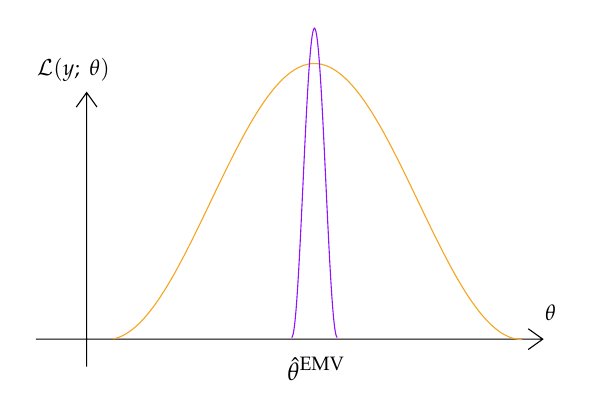
\begin{tikzpicture}[x=0.75pt,y=0.75pt,yscale=-1,xscale=1]
%uncomment if require: \path (0,300); %set diagram left start at 0, and has height of 300

%Shape: Axis 2D [id:dp33309643030277414] 
\draw  (48,169.8) -- (292.17,169.8)(72.42,51) -- (72.42,183) (285.17,164.8) -- (292.17,169.8) -- (285.17,174.8) (67.42,58) -- (72.42,51) -- (77.42,58)  ;
%Shape: Wave [id:dp761793702798415] 
\draw  [color={rgb, 255:red, 245; green, 166; blue, 35 }  ,draw opacity=1 ] (282.17,170) .. controls (264.07,170) and (248.47,137.57) .. (232.17,103.5) .. controls (215.86,69.43) and (200.26,37) .. (182.17,37) .. controls (164.07,37) and (148.47,69.43) .. (132.17,103.5) .. controls (116.77,135.67) and (102,166.38) .. (85.17,169.7) ;
%Shape: Wave [id:dp8411747217824341] 
\draw  [color={rgb, 255:red, 144; green, 19; blue, 254 }  ,draw opacity=1 ] (193.17,169) .. controls (191.18,169) and (189.46,132.67) .. (187.67,94.5) .. controls (185.87,56.33) and (184.16,20) .. (182.17,20) .. controls (180.18,20) and (178.46,56.33) .. (176.67,94.5) .. controls (174.87,132.67) and (173.16,169) .. (171.17,169) ;

% Text Node
\draw (183,184) node  [font=\small] [align=left] {$\displaystyle \hat{\theta}^{\text{EMV}}$};
% Text Node
\draw (296,157) node  [font=\footnotesize] [align=left] {$\displaystyle \theta $};
% Text Node
\draw (66,40) node  [font=\footnotesize] [align=left] {$\displaystyle \mathcal{L}( y;\ \theta )$};


\end{tikzpicture}

On peut donc voir que la forme de la fonction de vraisemblance est plus comprimée, alias que la concavité est plus forte, que l'autre fonction qui se maximise au même point. C'est-à-dire, la fonction de vraisemblance correspond à la fonction avec \textit{la plus forte concavité} dont le maximum est à $\hat{\theta}^{\text{EMV}}_{n}$.	\\

On peut observer que plus la concavité augmente, plus la variabilité de la fonction de vraisemblance se rapetisse. En effet, une faible concavité implique que la fonction de vraisemblance a un grand étendue de valeurs possibles et moins de points près de $\hat\theta^{\text{EMV}}$. En bref, \lfbox[imphl]{la deuxième dérivée assure que} parmi les fonctions se maximisant à $\hat{\theta}^{\text{EMV}}_{n}$, \lfbox[imphl]{la fonction de vraisemblance est celle dont la variabilité des prévisions est minimisée}.	\\

L'information de Fisher permet de quantifier cette fonction de la deuxième dérivée. Puis, la borne de Cramér-Rao se définit comme son réciproque $1 / \bm{I}(\theta)$. L'intuition est que plus la concavité est faible, plus l'étendue est grand. Prendre le réciproque de l'information de Fisher permet donc de quantifier l'agrandissement de l'étendu.\\

Lorsque l'information de Fisher tend vers l'infini (alias la force de la concavité croît infiniment), on dit que la distribution de l'estimateur est "asymptotiquement normale" tel que $\hat\theta^{\text{EMV}} \overset{a.s.}{\rightarrow} \mathcal{N}\Big(\mu = \theta, \sigma^{2} = \frac{1}{\bm{I}(\theta)}\Big)$ où a.s. veut dire \hyperlink{asympto}{asymptotiquement}.

\columnbreak
\subsubsection{Efficacité}
\begin{distributions}[Notation]
\begin{description}[font = \normalfont]
	\item[$\text{eff}(\hat{\theta}_{n})$]	Efficacité d'un estimateur $\hat{\theta}_{n}$;
	\item[$\text{eff}(\hat\theta_{n}, \tilde\theta_{n})$]	Efficacité de l'estimateur $\hat{\theta}_{n}$ relatif à l'estimateur $\tilde{\theta}_{n}$.
\end{description}
\end{distributions}

Avec le concept de l'information de Fisher, on définit \textbf{l'efficacité d'un estimateur} comme le ratio de la borne Cramér-Rao sur la variance de l'estimateur:
\begin{algo}{Efficacité d'un estimateur}
\begin{align*}
	\text{eff}(\hat{\theta}_{n})
	&=	\frac{\text{Var}(\hat{\theta}_{n})^{\text{Rao}}}{\text{Var}(\hat{\theta})} 
	=	\frac{1}{\bm{I}(\theta)\text{Var}(\hat{\theta})}
\end{align*}
\tcbline
\begin{description}
	\item[Estimateur \og \textit{efficient} \fg{}]	Lorsque la variance de l'estimateur $\text{Var}(\hat{\theta}_{n})$ est égale à la borne de Cramér-Rao.
		\begin{align*}
		\text{eff}(\hat{\theta}_{n}) = 1
		\end{align*}
	\begin{itemize}[leftmargin = *]
	\item	Étant égal à la borne, il \textit{doit} être l'estimateur avec la plus petite de tous les estimateurs sans biais.\\
	 		On dit qu'il est le \og \textbf{\textit{Minimum Variance Unbiased Estimator (MVUE)}} \fg{}. 
	\end{itemize}
\end{description}
\end{algo}

De plus, on peut généraliser cette formulation pour obtenir l'efficacité relative d'un estimateur à un autre:
\begin{algo}{Efficacité relative}
\begin{align*}
	\text{eff}(\hat\theta_{n}, \tilde\theta_{n})
	&=	\frac{\text{Var}(\hat\theta_{n})}{\text{Var}(\tilde\theta_{n})}		\\
\end{align*}
où les estimateurs $\hat\theta_{n}$ et $\tilde\theta_{n}$ sont sans biais.
\tcbline
Lorsque:
\begin{description}[font = \normalfont]
	\item[$\text{eff}(\hat\theta_{n}, \tilde\theta_{n}) < 1$:]	L'estimateur $\hat{\theta}_{n}$ est plus efficace que l'estimateur $\tilde{\theta}_{n}$, \\
	et vice-versa si $\text{eff}(\hat\theta_{n}, \tilde\theta_{n}) > 1$.
\end{description}
\end{algo}

\columnbreak
\subsubsection{Convergence}
Nous pouvons également évaluer si un estimateur converge avec des très grands échantillons; ceci évalue si un estimateur est cohérent. Un estimateur $\hat{\theta}_{n}$ est dit d'être \og \textit{\textbf{consistent}} \fg{} si la probabilité que sa prévision $\hat{\theta}$ du paramètre $\theta$ diffère de la vraie valeur par une erreur, près de 0, $\epsilon$ tend vers 0 alors que la taille de l'échantillon $n$ tend vers l'infini:
\begin{algo}{Convergence (\textbf{consistency}) d'un estimateur}
\begin{align*}
	\underset{n \rightarrow \infty}{\lim} \Pr(\big| \hat{\theta}_{n} - \theta \big| > \epsilon) = 0, \quad \epsilon > 0
\end{align*}
\end{algo}

Ce critère pour qu'un estimateur $\hat{\theta}_{n}$ soit \og \textit{consistent} \fg{} peut être satisfait lorsque: 
\begin{enumerate}
	\item	l'estimateur est \hypertarget{asympto}{\textbf{asymptotiquement sans biais}};
		\begin{align*}
		\limz{n}{\infty} \text{B}(\hat{\theta}_{n}) = 0
		\end{align*}
	\item	la \textbf{variance de l'estimateur tend vers 0}.
		\begin{align*}
		\limz{n}{\infty} \text{Var}(\hat{\theta}_{n}) = 0
		\end{align*}
\end{enumerate}

D'ailleurs, nous avons déjà raisonné ceci avec \hyperlink{cramer-rao}{la borne inférieure Cramér-Rao}.

Cependant, l'inverse n'est pas vrai---qu'un estimateur soit \og \textit{consistent} \fg{} n'implique pas que sa variance ni que son biais tendent vers 0.\\

Malgré la nature plaisante de la convergence d'un estimateur, beaucoup d'estimateurs ont cette propriété. 
Nous voulons alors une mesure qui n'indique pas seulement qu'un estimateur arrive près de la bonne valeur souvent \textit{(alias, une très petite variance)}, mais qu'il est mieux que d'autres estimateurs.
De plus, dût à la sélection arbitraire de l'erreur $\epsilon$ pour la \textit{consistency} d'un estimateur, il est possible de la choisir malicieusement afin de faire parler les données comme on le souhaite. 

\subsubsection*{Détails sur la convergence}
On reprend les résultats de la section précédente en expliquant plus en détail la mathématique sous-jacente.\\

\begin{definitionNOHFILLsub}[Convergence en probabilité]
\begin{distributions}[Notation]
\begin{description}
	\item[$\{Y_{n}\}$]	Séquence de variables aléatoires;
	\item[$Y$]	Variable aléatoire comprise dans $\{Y_{n}\}$.
\end{description}
\end{distributions}

On dit que $Y_{n}$ converge en probabilité à $Y$ si \lfbox[conditions]{$\forall \varepsilon > 0$}, 
\begin{align*}
	\limz{n}{\infty} \Pr\left[|Y_{n}	-	Y|	\geq	\varepsilon\right]	
	&=	0
\end{align*}
%%%	--------------------
%%%	NOTES:
%%%	+	\geq ou > ???
%%%	--------------------
ou de façon équivalente,
\begin{align*}
	\limz{n}{\infty} \Pr\left[|Y_{n}	-	Y|<	\varepsilon\right]	
	&=	1
\end{align*}

On dénote la convergence en probabilité par: \lfbox[formula]{$Y_{n}	\overset{P}{\rightarrow}	Y$.}
\end{definitionNOHFILLsub}

\paragraph{Note:}	La convergence en probabilité est d'ailleurs le théorème sous-jacent à la loi faible des grands nombres vue en prob.

\begin{rappel}{Loi faible des grands nombres}
\begin{distributions}[Notation]
\begin{description}
	\item[$\{Y_{n}\}$]	Séquence de variables aléatoires iid avec moyenne $\mu$ et variance $\sigma^{2}$ où \lfbox[conditions]{$\sigma^{2}	<	\infty$};
	\item[$\overline{X}_{n}$]	Moyenne empirique.
\end{description}
\end{distributions}

On pose que \lfbox[formula]{$\overline{X}_{n}	\overset{P}{\rightarrow}	\mu$.}
\end{rappel}

\begin{definitionNOHFILLsub}[Théorèmes résultant de la convergence en probabilité]
Soit \lfbox[conditions]{$X_{n}	\overset{P}{\rightarrow}	X$} et \lfbox[conditions]{$Y_{n}	\overset{P}{\rightarrow}	Y$}. Alors \lfbox[formula]{$X_{n} + Y_{n}	\overset{P}{\rightarrow}	X + Y$}.\\
Soit \lfbox[conditions]{$X_{n}	\overset{P}{\rightarrow}	X$} et une \lfbox[conditions]{constante $a$}. Alors \lfbox[formula]{$aX_{n}	\overset{P}{\rightarrow}	aX$}.\\
Soit \lfbox[conditions]{$X_{n}	\overset{P}{\rightarrow}	a$} et la \lfbox[conditions]{fonction $g(\cdot)$ continue à $a$}. Alors \lfbox[formula]{$g(X_{n})	\overset{P}{\rightarrow}	g(a)$}.\\
Soit \lfbox[conditions]{$X_{n}	\overset{P}{\rightarrow}	X$} et la \lfbox[conditions]{fonction continue $g(\cdot)$}. Alors \lfbox[formula]{$g(X_{n})	\overset{P}{\rightarrow}	g(X)$}.\\
Soit \lfbox[conditions]{$X_{n}	\overset{P}{\rightarrow}	X$} et \lfbox[conditions]{$Y_{n}	\overset{P}{\rightarrow}	Y$}. Alors \lfbox[formula]{$X_{n}Y_{n}	\overset{P}{\rightarrow}	XY$}.
\end{definitionNOHFILLsub}

\begin{definitionNOHFILL}[\og \textit{Consistency} \fg{}]
\begin{distributions}[Notation]
\begin{description}
	\item[$Y$]	Variable aléatoire avec une distribution paramétrique de paramètre $\theta$;
	\item[$\{Y_{1}, Y_{2}, \dots, Y_{n}\}$]	Échantillon de la distribution de $Y$;
	\item[$\hat{\theta}_{n}$]	Estimateur de $\theta$.
\end{description}
\end{distributions}

On dit que $\hat{\theta}_{n}$ est un estimateur \og \textit{consistent} \fg{} si \lfbox[formula]{$\hat{\theta}_{n}	\overset{P}{\rightarrow}	\theta$}.
\end{definitionNOHFILL}


\subsubsection{Erreur quadratique moyenne}
\begin{distributions}[Notation]
\begin{description}
	\item[$\text{MSE}_{\hat{\theta}_{n}}(\theta)$]	Erreur quadratique moyenne d'un estimateur $\hat{\theta}_{n}$
\end{description}
\end{distributions}

On défini alors l'\textbf{Erreur Quadratique Moyenne} (EQM), ou \textbf{Mean Squared Error (MSE)}, permettant de comparer les différents estimateurs ayant tous une bonne \textit{consistency} en assurant une cohérence d'interprétation. Cette mesure permet de quantifier l'écart entre un estimateur $\hat{\theta}_{n}$ et le vrai paramètre $\theta$.

\begin{algo}{Erreur Quadratique Moyenne (Mean Squared Error)}
\begin{align*}
	\text{MSE}_{\hat\theta}(\theta)
	&=	\text{E}[(\hat{\theta}_{n} - \theta)^{2}]
	\Leftrightarrow	\text{Var}(\hat{\theta}_{n}) + \left[\text{B}(\hat{\theta}_{n})\right]^{2}
\end{align*}
\end{algo}

En combinant tous ces critères, le meilleur estimateur est alors l'estimateur \textbf{sans biais} ayant la \textbf{plus petite variance} possible parmi tous les estimateurs \textit{sans biais}. C'est-à-dire, le \textbf{Uniformly Minimum Variance Unbiased Estimator \textit{(UMVUE)}}.

\columnbreak

\subsection{Estimation par intervalles}
\label{sec:int-estimation}
\begin{distributions}[Notation]
\begin{description}
	\item[$\hat{\theta}_{L}$ et $\hat{\theta}_{U}$]	Fonctions de l'échantillon aléatoire $\{X_{1}, \dots, X_{n}\}$ où \icbox[red][palechestnut]{$\hat{\theta}_{L} < \hat{\theta}_{U}$};
	\item[$(\hat{\theta}_{L}, \hat{\theta}_{U})$]	Intervalle de confiance de $100(1 - \alpha)\%$ de $\theta$ si \icbox[red][palechestnut]{$\Pr(\hat{\theta}_{L} \leq \theta \leq \hat{\theta}_{U}) = 1 - \alpha$};
		\begin{itemize}
		\item	Avec les réalisations, on a un intervalle de nombres réels $(\hat{\theta}_{l}, \hat{\theta}_{u})$.
		\end{itemize}
	\item[$(1 - \alpha)$]	Niveau de confiance de l'intervalle où \lfbox[conditions]{$\alpha \in (0, 1)$}.
\end{description}
\end{distributions}

Le type principal d'estimateur par intervalle est l'\textbf{intervalle de confiance}:
\begin{algo}{Intervalle de confiance}
Nous sommes confiants à un niveau de 100$(1 - \alpha)$\% que le paramètre inconnu $\theta$ est entre $(\hat{\theta}_{L}, \hat{\theta}_{U})$. 

De façon équivalente, nous sommes confiants à un seuil de $\alpha$\% que $\theta$ est entre $(\hat{\theta}_{L}, \hat{\theta}_{U})$.\\

Donc, \icbox{$\theta \in (\hat{\theta}_{L}, \hat{\theta}_{U})$} et nous pouvons dire que \icbox{$\Pr( \hat{\theta}_{L} \le \theta \le  \hat{\theta}_{U}) \ge (1 - \alpha)$} \icbox[red][palechestnut]{pour tout $\theta$}.
\end{algo}

Ce qu'il faut bien saisir avec les intervalles de confiance, c'est que \lfbox[imphl]{soit $\theta$ est contenu dans l'intervalle $(\hat{\theta}_{l}, \hat{\theta}_{u})$ ou il ne l'est pas}.

On peut conceptualiser les intervalles comme une distribution binomiale avec probabilité de succès de $(1 - \alpha)$. Si l'on effectue $M$ essais indépendants, on s'attend à ce que $(1 - \alpha)M$ intervalles de confiance contiennent $\theta$. Donc on se sent confiant à $(1 - \alpha)\%$ que la vraie valeur de $\theta$ est contenue dans l'intervalle observé $(\hat{\theta}_{l}, \hat{\theta}_{u})$.

\paragraph{Efficacité des intervalles de confiance}
Typiquement, la largeur de l'intervalle $(\hat{\theta}_{L}, \hat{\theta}_{U})$ augmente si on augmente le niveau de confiance $(1 - \alpha)$. Par exemple, pour être certain à 100\% que l'intervalle va contenir la valeur, on a qu'à faire un intervalle $(-\infty, \infty)$.\\

Donc, un intervalle plus petit nous donne plus d'information si le niveau est adéquat. On dit que pour un même niveau $(1 - \alpha)$, l'intervalle avec la plus petite largeur est \textit{plus efficace} que l'autre.



\columnbreak
\subsubsection{Statistiques}
\begin{rappel_enhanced}[Rappel : Loi du khi-carré]
Soit un échantillon aléatoire $(X_{1}, X_{2}, \dots, X_{n})$ de variables aléatoires normales de moyenne $\mu$ et variance $\sigma^{2}$.\\
Soit \lfbox[formula]{$Q	=	\sumz{n}{i	=	1}\left(X_{i}	-	\mu\right)^{2}$}.\\

Alors, \lfbox[formula]{$Q/\sigma^{2} \sim \chi^{2}_{(n)}$}.
\end{rappel_enhanced}

\begin{rappel_enhanced}[Rappel : Loi de Student]
Soit les variables aléatoires indépendantes :
\begin{itemize}
	\item	$Z \sim \mathcal{N}(0, 1)$.
	\item	$W \sim \chi^{2}_{(n)}$.
\end{itemize}

Alors, \lfbox[formula]{$T	=	\frac{Z}{\sqrt{W/n}}	\sim	t_{(n)}$}.\\

\tcbline

La loi de Student tend vers la normale lorsque $n$ est très grand.
\end{rappel_enhanced}

\begin{rappel_enhanced}[Rappel : Loi de Fisher-Snedecor ($F$)]
Soit les variables aléatoires indépendantes :
\begin{itemize}
	\item	$W_{1} \sim \chi^{2}_{(\nu_{1})}$.
	\item	$W_{2} \sim \chi^{2}_{(\nu_{2})}$.
\end{itemize}

Alors, \lfbox[formula]{$F	=	\frac{W_{1}/\nu_{1}}{W_{2}/\nu_{2}}	\sim	\mathcal{F}_{(\nu_{1}, \nu_{2})}$}.\\

\tcbline

On peut relier la loi de Student et la loi F : \lfbox[formula]{$T^{2}	=	\frac{Z^{2}}{W/n}	\sim	\mathcal{F}_{(1, n)}$} puisque \lfbox[formula]{$Z^{2} \sim \chi^{2}_{(1)}$} où \lfbox[conditions]{$Z \sim \mathcal{N}(0, 1)$}.
\end{rappel_enhanced}

\begin{definitionNOHFILL}[Statistique de test $T_{n}$]
$T_{n}$ est une statistique de test basée sur un échantillon aléatoire de $n$ observations.

\begin{itemize}
\item	C'est donc une \textbf{fonction} d'un échantillon aléatoire ;
\item	Sa distribution est la \textbf{distribution d'échantillonnage} qui dépend de :
	\begin{enumerate}
	\item	La statistique.
	\item	La taille de l'échantillon.
	\item	La distribution sous-jacente des données.
	\end{enumerate}
\end{itemize}
\end{definitionNOHFILL}

\begin{definitionNOHFILLprop}[Moyenne échantillonnale $\bar{X}$]
\lfbox[formula]{$\bar{X}	=	\frac{\sum^{n}_{i = 1} X_{i}}{n}$}.

\begin{itemize}
	\item	Estime sans biais la moyenne $\mu$ ;
	\item	Si on pose que l'échantillon aléatoire est normalement distribué, $\bar{X}	\sim \mathcal{N}(\mu, \frac{\sigma}{\sqrt{n}})$ ;
	\item	On centre et réduit pour trouver que \lfbox[formula]{$T_{n}	=	\frac{\bar{X} - \mu}{\sigma/\sqrt{n}} \sim \mathcal{N}(0, 1)$} ;
	\item	Si $\sigma^{2}$ est inconnue, on l'estime avec $s^{2}_{n}$ pour obtenir une distribution student---\lfbox[formula]{$T_{n}	=	\frac{\bar{X} - \mu}{S_{n}/\sqrt{n}}	=	\frac{Z}{\sqrt{W/(n - 1)}} \sim t_{(n - 1)}$} où $W \sim \chi^{2}_{(n - 1)}$.
\end{itemize}
\end{definitionNOHFILLprop}

\begin{definitionNOHFILLprop}[Variance échantillonnale $S^{2}_{n}$]
\lfbox[formula]{$S^{2}_{n}	=	\frac{\sum (X_{i} - \bar{X})^{2}}{n - 1}$}.

\begin{itemize}
	\item	Estime \underline{sans biais} la vraie variance $\sigma^{2}$ ;
	\item	$S^{2}_{n}$ n'est pas normalement distribuée, cependant la statistique \lfbox[formula]{$T_{n}	=	\frac{(n - 1)S^{2}_{n}}{\sigma^{2}} \sim \chi^{2}_{(n - 1)}$}.
\end{itemize}
\end{definitionNOHFILLprop}

\begin{definitionNOHFILLprop}[Variance empirique $\hat{\sigma}^{2}$]
\lfbox[formula]{$\hat{\sigma}^{2}	=	\frac{\sum (X_{i} - \bar{X})^{2}}{n}$}.

\begin{itemize}
	\item	Estime \underline{avec biais} la vraie variance $\sigma^{2}$.
\end{itemize}
\end{definitionNOHFILLprop}

\begin{definitionNOHFILLprop}[Statistique $F$]
\lfbox[formula]{$F	=	\frac{S^{2}_{n}/\sigma^{2}_{1}}{S^{2}_{m}/\sigma^{2}_{2}}$}.

\begin{itemize}
	\item	Si on pose que les deux échantillons aléatoires indépendants $(X_{1}, \dots, X_{n})$ et $(Y_{1}, \dots, Y_{m})$ sont normalement distribués, \lfbox[formula]{$F \sim \mathcal{F}_{(n - 1, m - 1)}$}.
\end{itemize}
\end{definitionNOHFILLprop}

\paragraph{Note sur majuscule vs minuscule}	On écrit les statistiques avec des majuscules lorsqu'elles sont aléatoires et avec des minuscules lorsque ce sont des réalisations. Par exemple, dans une probabilité on utilise une majuscule puisque la statistique est aléatoire. 
Pour un seuil $\alpha$ \textbf{\underline{fixé}} d'un intervalle de confiance, le quantile n'est pas aléatoire et jusqu'à ce que l'on calcule l'intervalle avec l'échantillon observé, les statistiques sont également aléatoires. 



\columnbreak
\subsubsection{Intervalles de confiance}
%
%De façon générale, les intervalles de confiance ont une estimation ponctuelle à laquelle on ajoute une marge d'erreur.

\begin{definitionNOHFILLsub}[Intervalle de confiance sur la variance]
%%%	https://www.youtube.com/watch?v=qwqB5a7_W44
Pour l'échantillon aléatoire $\{X_{1}, X_{2}, \dots, X_{n}\}$ issu d'une distribution normale avec $\sigma^{2}$ inconnue, \lfbox[formula]{$\Pr\left(\chi^{2}_{1 - \alpha/2} \leq \frac{(n - 1)S^{2}_{n}}{\sigma^{2}} \leq \chi^{2}_{\alpha/2}\right) =	(1 - \alpha)$}. \\

Graphiquement: 
\begin{center}
\tikzset{every picture/.style={line width=0.75pt}} %set default line width to 0.75pt        

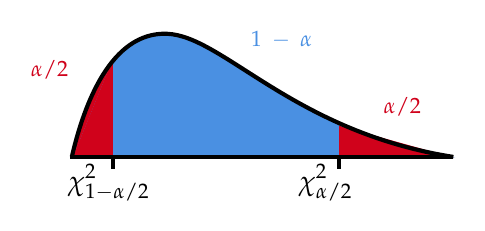
\begin{tikzpicture}[x=0.75pt,y=0.75pt,yscale=-1,xscale=1]
%uncomment if require: \path (0,300); %set diagram left start at 0, and has height of 300

%Curve Lines [id:da6253759692396421] 
\draw [draw opacity=0][fill={rgb, 255:red, 74; green, 144; blue, 226 }  ,fill opacity=1 ][line width=1.5]    (100.83,100.33) .. controls (106.67,75) and (119.67,40) .. (146.67,41) .. controls (173.67,42) and (207.67,88.33) .. (284.67,100.33) ;
%Straight Lines [id:da9705044831224325] 
\draw [draw opacity=0][fill={rgb, 255:red, 208; green, 2; blue, 27 }  ,fill opacity=1 ]   (119.83,52.67) -- (119.83,99.33) -- (100.83,99.33) ;
%Curve Lines [id:da9090824147972125] 
\draw [draw opacity=0][fill={rgb, 255:red, 208; green, 2; blue, 27 }  ,fill opacity=1 ][line width=2.25]    (100.83,99.33) .. controls (106.67,72) and (114.83,58.67) .. (119.83,52.67) ;

%Straight Lines [id:da8243679921312423] 
\draw [draw opacity=0][fill={rgb, 255:red, 208; green, 2; blue, 27 }  ,fill opacity=1 ]   (228.83,85) -- (228.83,100.33) -- (283.83,100.33) ;
%Curve Lines [id:da07655100443368612] 
\draw [line width=1.5]    (100,100) .. controls (105.83,74.67) and (118.83,39.67) .. (145.83,40.67) .. controls (172.83,41.67) and (206.83,88) .. (283.83,100) ;
%Straight Lines [id:da5824849118650262] 
\draw [line width=1.5]    (119.83,100.33) -- (119.83,105.67) ;
%Straight Lines [id:da7912407501617629] 
\draw [line width=1.5]    (228.83,100.33) -- (228.83,105.67) ;
%Straight Lines [id:da26335370673771696] 
\draw [line width=1.5]    (99,100) -- (283.83,100) ;

% Text Node
\draw (79,52) node [anchor=north west][inner sep=0.75pt]  [font=\footnotesize,color={rgb, 255:red, 208; green, 2; blue, 27 }  ,opacity=1 ] [align=left] {$\displaystyle \alpha /2$};
% Text Node
\draw (249,70) node [anchor=north west][inner sep=0.75pt]  [font=\footnotesize,color={rgb, 255:red, 208; green, 2; blue, 27 }  ,opacity=1 ] [align=left] {$\displaystyle \alpha /2$};
% Text Node
\draw (185,38) node [anchor=north west][inner sep=0.75pt]  [font=\footnotesize,color={rgb, 255:red, 74; green, 144; blue, 226 }  ,opacity=1 ] [align=left] {$\displaystyle 1\ -\ \alpha $};
% Text Node
\draw (96.83,102.33) node [anchor=north west][inner sep=0.75pt]   [align=left] {$\displaystyle \chi ^{2}_{1-\alpha /2}$};
% Text Node
\draw (208,102.33) node [anchor=north west][inner sep=0.75pt]   [align=left] {$\displaystyle \chi ^{2}_{\alpha /2}$};


\end{tikzpicture}
\end{center}

Nous sommes donc confiants à un niveau de 100$(1 - \alpha)$\% que :
\begin{align*}
	\sigma^{2} \in \left[
		\frac{(n - 1)S^{2}_{n}}{\chi^{2}_{\alpha / 2}}, 
		\frac{(n - 1)S^{2}_{n}}{\chi^{2}_{1 - \alpha / 2}}
	\right]
\end{align*}
\end{definitionNOHFILLsub}

\begin{definitionNOHFILLsub}[Intervalle de confiance sur la moyenne ($\sigma^{2}$ connue)]
%%%	https://www.youtube.com/watch?v=KG921rfbTDw&list=PLvxOuBpazmsMdPBRxBTvwLv5Lhuk0tuXh&index=4&t=0s
%%%	https://www.youtube.com/watch?v=-iYDu8flFXQ&list=PLvxOuBpazmsMdPBRxBTvwLv5Lhuk0tuXh&index=3&t=268s
Pour l'échantillon aléatoire $\{X_{1}, X_{2}, \dots, X_{n}\}$ issu d'une distribution normale avec $\mu$ inconnu et $\sigma^{2}$ connue, \lfbox[formula]{$\Pr\left(-z_{\alpha/2} \leq \frac{\bar{X} - \mu}{\sigma/\sqrt{n}} \leq z_{\alpha/2}\right) =	(1 - \alpha)$}.\\

Graphiquement:
\begin{center}


\tikzset{every picture/.style={line width=0.75pt}} %set default line width to 0.75pt        

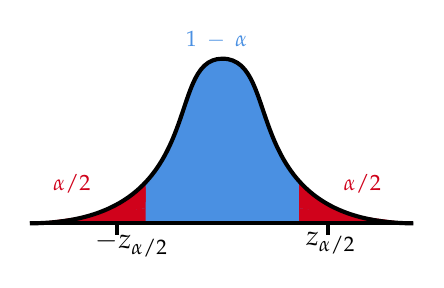
\begin{tikzpicture}[x=0.75pt,y=0.75pt,yscale=-1,xscale=1]
%uncomment if require: \path (0,176); %set diagram left start at 0, and has height of 176

%Curve Lines [id:da8947130044196236] 
\draw [draw opacity=0][fill={rgb, 255:red, 74; green, 144; blue, 226 }  ,fill opacity=1 ][line width=1.5]    (387,99) .. controls (474.83,98.67) and (450.83,19.67) .. (479.83,19.67) .. controls (509.83,19.67) and (485.83,98.67) .. (571.83,99) ;
%Straight Lines [id:da8407133508917781] 
\draw [line width=1.5]    (428.83,99.33) -- (428.83,104.67) ;
%Straight Lines [id:da7153733396293662] 
\draw [line width=1.5]    (530.83,99.33) -- (530.83,104.67) ;
%Straight Lines [id:da1468161753341053] 
\draw [draw opacity=0][fill={rgb, 255:red, 208; green, 2; blue, 27 }  ,fill opacity=1 ]   (516.83,91.67) -- (516.83,99) -- (571.83,99) ;
%Straight Lines [id:da44372694181119354] 
\draw [draw opacity=0][fill={rgb, 255:red, 208; green, 2; blue, 27 }  ,fill opacity=1 ]   (516.83,81.67) -- (516.83,91.67) -- (540.5,95.67) ;
%Straight Lines [id:da871067588661014] 
\draw [draw opacity=0][fill={rgb, 255:red, 208; green, 2; blue, 27 }  ,fill opacity=1 ]   (516.83,78.67) -- (516.83,88.67) -- (528.67,93.67) ;

%Straight Lines [id:da7000317622260974] 
\draw [draw opacity=0][fill={rgb, 255:red, 208; green, 2; blue, 27 }  ,fill opacity=1 ]   (442.83,91.67) -- (442.83,99) -- (387.83,99) ;
%Straight Lines [id:da8176903889743383] 
\draw [draw opacity=0][fill={rgb, 255:red, 208; green, 2; blue, 27 }  ,fill opacity=1 ]   (442.83,81.67) -- (442.83,91.67) -- (419.17,95.67) ;
%Straight Lines [id:da7955659226488763] 
\draw [draw opacity=0][fill={rgb, 255:red, 208; green, 2; blue, 27 }  ,fill opacity=1 ]   (442.83,78.67) -- (442.83,88.67) -- (431,93.67) ;

%Curve Lines [id:da21189166086741196] 
\draw [line width=1.5]    (387,99) .. controls (474.83,98.67) and (450.83,19.67) .. (479.83,19.67) .. controls (509.83,19.67) and (485.83,98.67) .. (571.83,99) ;
%Straight Lines [id:da9615401029487891] 
\draw [line width=1.5]    (387,99) -- (571.83,99) ;


% Text Node
\draw (397,74) node [anchor=north west][inner sep=0.75pt]  [font=\footnotesize,color={rgb, 255:red, 208; green, 2; blue, 27 }  ,opacity=1 ] [align=left] {$\displaystyle \alpha /2$};
% Text Node
\draw (537,74) node [anchor=north west][inner sep=0.75pt]  [font=\footnotesize,color={rgb, 255:red, 208; green, 2; blue, 27 }  ,opacity=1 ] [align=left] {$\displaystyle \alpha /2$};
% Text Node
\draw (461,5) node [anchor=north west][inner sep=0.75pt]  [font=\footnotesize,color={rgb, 255:red, 74; green, 144; blue, 226 }  ,opacity=1 ] [align=left] {$\displaystyle 1\ -\ \alpha $};
% Text Node
\draw (518.83,102) node [anchor=north west][inner sep=0.75pt]   [align=left] {$\displaystyle z_{\alpha /2}$};
% Text Node
\draw (417.33,102) node [anchor=north west][inner sep=0.75pt]   [align=left] {$\displaystyle -z_{\alpha /2}$};


\end{tikzpicture}
\end{center}


Nous sommes donc confiants à un niveau de 100$(1 - \alpha)$\% que :
\begin{equation*}
	\mu \in \left[ \bar{X} - z_{\alpha/2} \frac{\sigma}{\sqrt{n}}, \bar{X} + z_{\alpha/2} \frac{\sigma}{\sqrt{n}}\right].
\end{equation*}
\end{definitionNOHFILLsub}

\begin{definitionNOHFILLsub}[Intervalle de confiance sur la moyenne ($\sigma^{2}$ inconnue)]
Pour l'échantillon aléatoire $\{X_{1}, X_{2}, \dots, X_{n}\}$ issu d'une distribution normale avec $\sigma^{2}$ inconnue, \lfbox[formula]{$\Pr\left(-t_{\alpha/2, n - 1} \leq \frac{\bar{X} - \mu}{S_{n}/\sqrt{n}} \leq t_{\alpha/2, n - 1}\right) =	(1 - \alpha)$}.\\

Graphiquement:
\begin{center}
\tikzset{every picture/.style={line width=0.75pt}} %set default line width to 0.75pt        

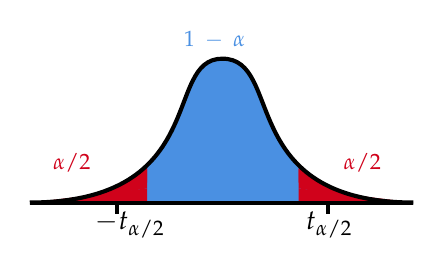
\begin{tikzpicture}[x=0.75pt,y=0.75pt,yscale=-1,xscale=1]
%uncomment if require: \path (0,176); %set diagram left start at 0, and has height of 176

%Curve Lines [id:da982458578172261] 
\draw [draw opacity=0][fill={rgb, 255:red, 74; green, 144; blue, 226 }  ,fill opacity=1 ][line width=1.5]    (386,98) .. controls (473.83,97.67) and (449.83,28.67) .. (478.83,28.67) .. controls (508.83,28.67) and (484.83,97.67) .. (570.83,98) ;
%Straight Lines [id:da3849016484089105] 
\draw [line width=1.5]    (427.83,98.33) -- (427.83,103.67) ;
%Straight Lines [id:da40648686188300065] 
\draw [line width=1.5]    (529.83,98.33) -- (529.83,103.67) ;
%Straight Lines [id:da0901743854683843] 
\draw [draw opacity=0][fill={rgb, 255:red, 208; green, 2; blue, 27 }  ,fill opacity=1 ]   (515.5,91.15) -- (515.5,98) -- (570.83,98) ;
%Straight Lines [id:da7611083055876529] 
\draw [draw opacity=0][fill={rgb, 255:red, 208; green, 2; blue, 27 }  ,fill opacity=1 ]   (515.5,81.8) -- (515.5,91.15) -- (539.31,94.89) ;
%Straight Lines [id:da39003595249115297] 
\draw [draw opacity=0][fill={rgb, 255:red, 208; green, 2; blue, 27 }  ,fill opacity=1 ]   (515.5,79) -- (515.5,88.34) -- (527.41,93.02) ;

%Straight Lines [id:da438403114586448] 
\draw [draw opacity=0][fill={rgb, 255:red, 208; green, 2; blue, 27 }  ,fill opacity=1 ]   (442.5,91.15) -- (442.5,98) -- (386.83,98) ;
%Straight Lines [id:da963730012359405] 
\draw [draw opacity=0][fill={rgb, 255:red, 208; green, 2; blue, 27 }  ,fill opacity=1 ]   (442.5,81.8) -- (442.5,91.15) -- (418.55,94.89) ;
%Straight Lines [id:da7346871172050706] 
\draw [draw opacity=0][fill={rgb, 255:red, 208; green, 2; blue, 27 }  ,fill opacity=1 ]   (442.5,79) -- (442.5,88.34) -- (430.52,93.02) ;

%Curve Lines [id:da971478425929696] 
\draw [line width=1.5]    (386,98) .. controls (473.83,97.67) and (449.83,28.67) .. (478.83,28.67) .. controls (508.83,28.67) and (484.83,97.67) .. (570.83,98) ;
%Straight Lines [id:da9295821978585093] 
\draw [line width=1.5]    (386,98) -- (570.83,98) ;

% Text Node
\draw (396,73) node [anchor=north west][inner sep=0.75pt]  [font=\footnotesize,color={rgb, 255:red, 208; green, 2; blue, 27 }  ,opacity=1 ] [align=left] {$\displaystyle \alpha /2$};
% Text Node
\draw (536,73) node [anchor=north west][inner sep=0.75pt]  [font=\footnotesize,color={rgb, 255:red, 208; green, 2; blue, 27 }  ,opacity=1 ] [align=left] {$\displaystyle \alpha /2$};
% Text Node
\draw (459,14) node [anchor=north west][inner sep=0.75pt]  [font=\footnotesize,color={rgb, 255:red, 74; green, 144; blue, 226 }  ,opacity=1 ] [align=left] {$\displaystyle 1\ -\ \alpha $};
% Text Node
\draw (517.83,101) node [anchor=north west][inner sep=0.75pt]   [align=left] {$\displaystyle t_{\alpha /2}$};
% Text Node
\draw (416.33,101) node [anchor=north west][inner sep=0.75pt]   [align=left] {$\displaystyle -t_{\alpha /2}$};


\end{tikzpicture}
\end{center}

Nous sommes donc confiants à un niveau de 100$(1 - \alpha)$\% que :
\begin{equation*}
	\mu \in \left[ \bar{X} - t_{\alpha/2, n - 1} \frac{S_{n}}{\sqrt{n}}, \bar{X} + t_{\alpha/2, n - 1} \frac{S_{n}}{\sqrt{n}}\right].
\end{equation*}
\end{definitionNOHFILLsub}


%%%	-------------------------
%%%	NOTES:
%%%	+	À retravailler cette section pour ajouter un peu plus de contexte sur les grands échantillons
%%%	-------------------------


\begin{definitionNOHFILLsub}[Intervalle de confiance \textit{approximatif} sur la moyenne]
%%%	https://www.youtube.com/watch?v=bFefxSE5bmo&list=PLvxOuBpazmsMdPBRxBTvwLv5Lhuk0tuXh&index=8&t=0s
Pour l'échantillon aléatoire $\{X_{1}, X_{2}, \dots, X_{n}\}$ issu d'une distribution avec moyenne $\mu$ et une variance inconnue.\\

Pour $n$ très grand, nous sommes \textit{approximativement} confiants à un niveau de 100$(1 - \alpha)$\% que :
\begin{equation*}
	\mu \in \left[ \bar{X} - z_{\alpha/2} \frac{s}{\sqrt{n}}, \bar{X} + z_{\alpha/2} \frac{s}{\sqrt{n}}\right].
\end{equation*}
\end{definitionNOHFILLsub}

\begin{definitionNOHFILLsub}[Intervalle de confiance \textit{approximatif} sur la proportion]
Pour l'échantillon aléatoire $\{X_{1}, X_{2}, \dots, X_{n}\}$ issu d'une distribution Bernoulli de paramètre $p$.\\

Pour $n$ très grand, nous sommes \textit{approximativement} confiants à un niveau de 100$(1 - \alpha)$\% que :
\begin{equation*}
	p \in \left[ \hat{p} - z_{\alpha/2} \sqrt{\frac{\hat{p}(1 - \hat{p})}{n}}, \hat{p} + z_{\alpha/2} \sqrt{\frac{\hat{p}(1 - \hat{p})}{n}}\right].
\end{equation*}
\end{definitionNOHFILLsub}

On définit le \og \textit{pooled estimator} \fg{} comme la moyenne pondérée des deux variances échantillonnales \lfbox[formula]{$S_{p}^{2}	=	\frac{(n - 1)S_{n}^{2} + (m - 1)S_{m}^{2}}{n + m - 2}$}.\\


\begin{definitionNOHFILLsub}[Intervalle de confiance pour une différence de moyennes]
Pour les échantillons aléatoires $\{X_{1}, X_{2}, \dots, X_{n}\}$ et $\{Y_{1}, Y_{2}, \dots, Y_{m}\}$ issus de distributions normales de moyennes $\mu_{1}$ et $\mu_{2}$ et variance $\sigma^{2}_{1} = \sigma^{2}_{2} = \sigma^{2}$ inconnues.

Nous sommes confiants à un niveau de 100$(1 - \alpha)$\% que :
\begin{equation*}
	(\mu_{1}	-	\mu_{2}) \in \left[ 
	\bar{x}_{n}	-	\bar{y}_{m}
	\pm	t_{\alpha/2, n + m - 2} S_{p}\sqrt{\frac{1}{n} + \frac{1}{m}} \right].
\end{equation*}
\begin{align*}
\end{align*}
\end{definitionNOHFILLsub}

\begin{definitionNOHFILLsub}[Intervalle de confiance \textit{approximatif} pour une différence de moyennes]
Pour les échantillons aléatoires $\{X_{1}, X_{2}, \dots, X_{n}\}$ et $\{Y_{1}, Y_{2}, \dots, Y_{m}\}$ issus de distributions normales de moyennes $\mu_{1}$ et $\mu_{2}$ et variances $\sigma^{2}_{1}$ et $\sigma^{2}_{2}$ inconnues.\\

Pour $n$ très grand, nous sommes \textit{approximativement} confiants à un niveau de 100$(1 - \alpha)$\% que :
\begin{equation*}
	(\mu_{1}	-	\mu_{2}) \in \left[ 
	\bar{X}_{n}	-	\bar{Y}_{m}
	\pm	z_{\alpha/2} \sqrt{\frac{S_{n}^{2}}{n} + \frac{S_{m}^{2}}{m}} \right].
\end{equation*}
\begin{align*}
\end{align*}
\end{definitionNOHFILLsub}

\begin{definitionNOHFILLsub}[Intervalle de confiance \textit{approximatif} pour une différence de proportions]
Pour les échantillons aléatoires $\{X_{1}, X_{2}, \dots, X_{n}\}$ et $\{Y_{1}, Y_{2}, \dots, Y_{m}\}$ issus de distributions Bernoulli de paramètres $p_{1}$ et $p_{2}$.\\

Pour $n$ très grand, nous sommes \textit{approximativement} confiants à un niveau de 100$(1 - \alpha)$\% que :
\begin{equation*}
	(p_{1}	-	p_{2}) \in \left[ 
	\hat{p}_{1}	-	\hat{p}_{2}
	\pm	z_{\alpha/2} \sqrt{\frac{\hat{p}_{1}(1 - \hat{p}_{1})}{n} + \frac{\hat{p}_{2}(1 - \hat{p}_{2})}{m}} \right].
\end{equation*}
\begin{align*}
\end{align*}
\end{definitionNOHFILLsub}


%%%
%%%	Méthode du pivot
%%%

\columnbreak
\section{Tests d'hypothèses}
\label{sec:hyp-test}
\subsection{Introduction}
\begin{rappel_enhanced}[Contexte]
Les statistiques classiques posent que tout phénomène observable est régi par un \textit{"\textbf{processus}" sous-jacent}.\\
On ne peut jamais savoir exactement ce qu'est ce "processus"; le mieux que l'on peut faire est d'émettre des \textit{\textbf{hypothèses}} vraisemblables sur ce qu'il pourrait être. \\
Par la suite, on analyse les observations en présumant qu'elles sont régies par le processus hypothétique et détermine la \textit{\textbf{vraisemblance des observations}}. On accepte le processus hypothétique si la vraisemblance est suffisamment élevée.
\end{rappel_enhanced}

\begin{distributions}[Notation]
\begin{description}
	\item[$\Theta_{0}$ et $\Theta_{1}$]	Sous-ensembles disjoints de $\Theta$ tel que \lfbox[formula]{$\Theta_{0} \cup \Theta_{1}	=	\Theta$;}
	\item[$\textrm{H}_{0}$]	Hypothèse nulle ;
		\begin{itemize}
		\item	Représente généralement le statu quo jusqu'à preuve contraire.
		\end{itemize}
	\item[$\textrm{H}_{1}$]	Hypothèse alternative.
		\begin{itemize}
		\item	Représente généralement un changement du statu quo.
		\end{itemize}
\end{description}
\end{distributions}

\begin{definitionNOHFILL}[Test d'hypothèse]
On spécifie une \textcolor{burntorange}{hypothèse} nulle et par conséquent une hypothèse alternative :
\begin{align*}
	\textrm{H}_{0}
	&:	\theta \in \Theta_{0}	&
	&\text{vs}	&
	\textrm{H}_{1}
	&:	\theta \in \Theta_{1}	\\
\end{align*}

Puis, on spécifie une \textcolor{orange-red}{expérience} et un \textcolor{orange}{test} pour décider si l'on accepte ou rejette l'hypothèse nulle.
\end{definitionNOHFILL}

\begin{distributions}[Terminologie]
\begin{description}
\item[\hypertarget{hyp-simple}{Hypothèse simple}]	Spécifie \textbf{entièrement} une distribution de probabilité.
	\begin{itemize}
	\item	Par exemple, $\mathcal{H}_{0}	:	q = 0.50$---on connaît la valeur exacte du paramètre $q$ pour une distribution Bernoulli.
	\end{itemize}
\item[Hypothèse composite]	Spécifie \textbf{partiellement} une distribution de probabilité.
	\begin{itemize}
	\item	Par exemple, $\mathcal{H}_{1}	:	q \neq 0.50$.---on ne connaît pas la valeur exacte du paramètre $q$, il pourrait être n'importe quel chiffre sauf $0.50$.
	\end{itemize}
\end{description}
\end{distributions}

\begin{formula}{Exemple du laissez-passer universitaire (LPU)}
\textcolor{orange-red}{Par exemple}, on veut savoir si les étudiants utilisent l'autobus (oui ou non) avant et après l'implantation du LPU.\\ 
On \textcolor{burntorange}{pose} que la proportion des gens qui utilisent l'autobus est $q	=	0.44$.\\
Il y a deux types de \textcolor{orange}{tests} qu'on peut faire,
\begin{itemize}
	\item	Tester si l'utilisation est différente est un test "\textbf{bilatéral}", car on teste si elle a augmenté \textit{ou} diminuée;
		\begin{align*}
		\textrm{H}_{0}
		&:	q	=	0.44	&
		\textrm{H}_{1}
		&:	q	\neq	0.44
		\end{align*}
	\item	Tester si l'utilisation a augmenté est un test "\textbf{unilatéral}", car on teste uniquement si elle a augmenté.
		\begin{align*}
		\textrm{H}_{0}
		&:	q	=	0.44	&
		\textrm{H}_{1}
		&:	q	>	0.44
		\end{align*}
\end{itemize}

Un test unilatéral requiert que l'on sache déjà que la proportion de gens "\textit{doit}" être supérieure. Un test bilatéral est plus conservatif et test les deux possibilités, il devrait donc être celui qu'on applique par défaut. \\

L'hypothèse :
\begin{description}
	\item[nulle]		dans les deux cas est que, en moyenne, l'utilisation de l'autobus n'a pas \textit{changée}. 
	\item[alternative]	dans le cas d'un test :
		\begin{description}
		\item[unilatéral]	est que, en moyenne, l'utilisation a \textit{augmentée}.
		\item[bilatéral]	est que, en moyenne, l'utilisation a \textit{changée}.
		\end{description}
\end{description}
\end{formula}

\begin{definitionNOHFILLsub}[Région critique]
\begin{distributions}[Notation]
\begin{description}
	\item[$\mathcal{S}$]	"Ensemble" de tous les résultats possible pour l'échantillon aléatoire;
	\item[$\mathcal{C}$]	\textbf{Région critique} du test qui est un sous-ensemble de $\mathcal{S}$.
\end{description}
\end{distributions}

On rejette $\textrm{H}_{0}$ si $\{X_{1}, \dots, X_{n}\} \in \mathcal{C}$.\\
On conserve $\textrm{H}_{0}$ si $\{X_{1}, \dots, X_{n}\} \in \mathcal{C}^{c}$.

\begin{itemize}
	\item	On peut aussi dire \og \textbf{région de rejet} \fg{}.
\end{itemize}
\end{definitionNOHFILLsub}

\begin{formula}{Exemple du laissez-passer universitaire (LPU)}
On reprend l'exemple du LPU.\\
L'ensemble des résultats possibles est $\mathcal{S} = [0, 1]$.
\begin{itemize}
	\item	Un test "\textbf{bilatéral}" a comme région critique $\mathcal{C} = [0, 0.44) \cup (0.44, 1]$;
	\item	Un test "\textbf{unilatéral}" testant l'augmentation a comme région critique $\mathcal{C} = (0.44, 1]$.
\end{itemize}
\end{formula}

On peut donc faire 2 types d'erreurs:
%%	voir les images que j'ai gardé pour quand je retouche à la matrice de confusion dans les GLMs pour développer et parler des métriques ! 
\begin{center}
\tikzset{every picture/.style={line width=0.75pt}} %set default line width to 0.75pt        

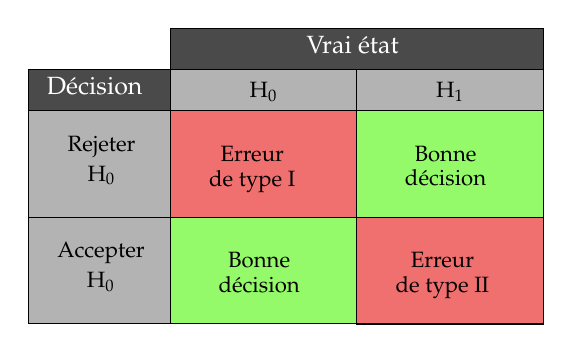
\begin{tikzpicture}[x=0.75pt,y=0.75pt,yscale=-1,xscale=1]
%uncomment if require: \path (0,165); %set diagram left start at 0, and has height of 165

%Shape: Rectangle [id:dp5658804967739193] 
\draw  [fill={rgb, 255:red, 240; green, 111; blue, 111 }  ,fill opacity=1 ] (74,50.17) -- (163.83,50.17) -- (163.83,101.5) -- (74,101.5) -- cycle ;
%Shape: Rectangle [id:dp933461228347003] 
\draw  [fill={rgb, 255:red, 240; green, 111; blue, 111 }  ,fill opacity=1 ] (163.83,101.5) -- (253.67,101.5) -- (253.67,152.83) -- (163.83,152.83) -- cycle ;
%Shape: Rectangle [id:dp24194313951746427] 
\draw  [fill={rgb, 255:red, 148; green, 250; blue, 106 }  ,fill opacity=1 ] (163.83,50) -- (253.67,50) -- (253.67,101.33) -- (163.83,101.33) -- cycle ;
%Shape: Rectangle [id:dp27324261874552724] 
\draw  [fill={rgb, 255:red, 148; green, 250; blue, 106 }  ,fill opacity=1 ] (74,101.33) -- (163.83,101.33) -- (163.83,152.67) -- (74,152.67) -- cycle ;
%Shape: Rectangle [id:dp9425087952138109] 
\draw  [fill={rgb, 255:red, 179; green, 179; blue, 179 }  ,fill opacity=1 ] (74,30.17) -- (163.83,30.17) -- (163.83,50) -- (74,50) -- cycle ;
%Shape: Rectangle [id:dp40513736937576916] 
\draw  [fill={rgb, 255:red, 74; green, 74; blue, 74 }  ,fill opacity=1 ] (74,10.33) -- (253.67,10.33) -- (253.67,30.17) -- (74,30.17) -- cycle ;
%Shape: Rectangle [id:dp4099498200973881] 
\draw  [fill={rgb, 255:red, 179; green, 179; blue, 179 }  ,fill opacity=1 ] (163.83,30.17) -- (253.67,30.17) -- (253.67,50) -- (163.83,50) -- cycle ;
%Shape: Rectangle [id:dp35293578825776084] 
\draw  [fill={rgb, 255:red, 179; green, 179; blue, 179 }  ,fill opacity=1 ] (5.5,101.33) -- (74,101.33) -- (74,152.67) -- (5.5,152.67) -- cycle ;
%Shape: Rectangle [id:dp2841127241620307] 
\draw  [fill={rgb, 255:red, 179; green, 179; blue, 179 }  ,fill opacity=1 ] (5.5,50.17) -- (74,50.17) -- (74,101.5) -- (5.5,101.5) -- cycle ;
%Shape: Rectangle [id:dp5918283025493905] 
\draw  [fill={rgb, 255:red, 74; green, 74; blue, 74 }  ,fill opacity=1 ] (5.5,30.33) -- (74,30.33) -- (74,50.17) -- (5.5,50.17) -- cycle ;

% Text Node
\draw (138.33,13) node [anchor=north west][inner sep=0.75pt]  [font=\small,color={rgb, 255:red, 255; green, 255; blue, 255 }  ,opacity=1 ] [align=left] {Vrai état};
% Text Node
\draw (110.92,35) node [anchor=north west][inner sep=0.75pt]  [font=\footnotesize,color={rgb, 255:red, 0; green, 0; blue, 0 }  ,opacity=1 ] [align=left] {$ \text{H}_{0}$};
% Text Node
\draw (200.75,35) node [anchor=north west][inner sep=0.75pt]  [font=\footnotesize,color={rgb, 255:red, 0; green, 0; blue, 0 }  ,opacity=1 ] [align=left] {$ \text{H}_{1}$};
% Text Node
\draw (18.25,112) node [anchor=north west][inner sep=0.75pt]  [font=\footnotesize,color={rgb, 255:red, 0; green, 0; blue, 0 }  ,opacity=1 ] [align=left] {\shortstack{Accepter\\ $\text{H}_{0}$}};
% Text Node
\draw (23.25,60.83) node [anchor=north west][inner sep=0.75pt]  [font=\footnotesize,color={rgb, 255:red, 0; green, 0; blue, 0 }  ,opacity=1 ] [align=left] {\shortstack{Rejeter\\ $\text{H}_{0}$}};
% Text Node
\draw (13.25,32.75) node [anchor=north west][inner sep=0.75pt]  [font=\small,color={rgb, 255:red, 255; green, 255; blue, 255 }  ,opacity=1 ] [align=left] {Décision};
% Text Node
\draw (91.42,65.83) node [anchor=north west][inner sep=0.75pt]  [font=\footnotesize,color={rgb, 255:red, 0; green, 0; blue, 0 }  ,opacity=1 ] [align=left] 
{\shortstack{Erreur\\ de type I}};
% Text Node
\draw (181.25,117) node [anchor=north west][inner sep=0.75pt]  [font=\footnotesize,color={rgb, 255:red, 0; green, 0; blue, 0 }  ,opacity=1 ] [align=left] {\shortstack{Erreur\\ de type II}};
% Text Node
\draw (95.92,117) node [anchor=north west][inner sep=0.75pt]  [font=\footnotesize,color={rgb, 255:red, 0; green, 0; blue, 0 }  ,opacity=1 ] [align=left] {\shortstack{Bonne\\ décision}};
% Text Node
\draw (185.75,65.67) node [anchor=north west][inner sep=0.75pt]  [font=\footnotesize,color={rgb, 255:red, 0; green, 0; blue, 0 }  ,opacity=1 ] [align=left] {\shortstack{Bonne\\ décision}};



\end{tikzpicture}
\end{center}

\columnbreak
\subsection{Certitude du test}
Lorsque nous voulons quantifier le degré auquel nous sommes confiants du test, nous utilisons la valeur $p$. \\
La valeur $p$ a trois composantes:
\begin{enumerate}
	\item	La probabilité que l'événement se produise aléatoirement.
	\item	La probabilité qu'un événement tout aussi rare se produise.
	\item	La probabilité qu'un événement encore plus rare se produise.
\end{enumerate}

\begin{formula}{Exemple de pile ou face}
On souhaite tester si, en obtenant deux piles sur deux lancers, nous avons une pièce de monnaie truquée :
\begin{description}
	\item[Hypothèse nulle]	Ma pièce de monnaie n'est pas truquée même si j'ai obtenu deux piles.
\end{description}
\

Étapes du calcul de la valeur $p$:
\begin{enumerate}
	\item	On calcule la probabilité d'obtenir 2 piles: $0.5 \times 0.5 = 0.25$.
	\item	Puis, on calcule la probabilité d'obtenir 2 faces (un événement tout aussi rare): $0.5 \times 0.5 = 0.25$.
	\item	Finalement, il n'y a pas d'autres séquences plus rares.
\end{enumerate}
Donc, la valeur $p$ du test est de $0.50$.

\begin{itemize}
	\item	Ceci est plutôt élevé;
	\item	Souvent, on pose que la valeur $p$ du test doit être d'au plus $0.05$;
	\item	Ce qui veut dire que des événements tout aussi (ou plus) rares doivent arriver moins que 5\% du temps pour que l'on considère la pièce de monnaie comme étant truquée;
	\item	Donc, dans notre cas, on ne peut pas rejeter l'hypothèse nulle que notre pièce de monnaie n'est pas spéciale.
\end{itemize}
\end{formula}

Dans le cas continu, on somme les probabilités d'être plus rare ou d'être moins rare. C'est la même idée que les intervalles de confiance avec la valeur $p$, ou \textit{seuil de signifiance $\alpha$}, représenté en rouge. 
\begin{itemize}
	\item	Si la valeur $p$ est petite, ceci indique que d'autres distributions pourraient potentiellement mieux s'ajuster aux données puisque l'événement est très rare;
	\item	Si la valeur $p$ est grande, ceci indique que l'événement est très courant et que la distribution semble être bien ajustée.
\end{itemize}

\

Il y a plusieurs termes semblables qui peuvent devenir mélangeants.
\begin{distributions}[Terminologie]
\begin{description}
	\item[$p$]	La \textbf{valeur $p$} du test.
		\begin{itemize}
		\item	On peut la définir comme la probabilité d'un événement tout aussi (ou plus) rare sous l'hypothèse nulle ;
		\item	On peut la définir comme la \textbf{taille} de la région critique $\mathcal{C}$ ; c'est-à-dire, l'\textit{aire} de la région de rejet de l'hypothèse nulle $\text{H}_{0}$ alors qu'elle est vraie ;
		\item	On peut la définir comme le \textbf{seuil de signifiance} ; c'est-à-dire, la probabilité de rejeter $\text{H}_{0}$ alors qu'elle est vraie ;
		\item	Elle correspond donc également à la \textbf{probabilité d'une erreur de type I}.
		\end{itemize}
	\item[$\alpha$]	Dénote habituellement le \textbf{seuil de signifiance} ou la \textbf{taille} du test.
		\begin{itemize}
		\item	Même idée qu'avec les intervalles de confiance;
		\item	On peut parfois aussi utiliser $\alpha$ pour dénoter la valeur de $p$ qui détermine si on rejette ou pas un test ;
		\item	En anglais, \og \textit{threshold for significance} \fg{}.
		\end{itemize}
\end{description}
\end{distributions}

Formellement, on définit \lfbox[formula]{$\alpha	=	{\color{indigo(web)}\max}_{{\color{amethyst}\theta} \in {\color{pastelred}\Theta_{0}}} \Pr\left\{{\color{bondiblue!80!black}(X_{1}, \dots, X_{n})} {\color{armygreen}\in} {\color{bulgarianrose}\mathcal{C}} ; {\color{amethyst}\theta} \right\}$}. \\
C'est-à-dire :
\begin{itemize}
	\item	on \textcolor{indigo(web)}{maximise} la probabilité que \textcolor{bondiblue!80!black}{l'échantillon aléatoire} soit \textcolor{armygreen}{contenu} dans \textcolor{bulgarianrose!90!black}{la région critique} (alias rejeter $\textrm{H}_{0}$), 
	\item	où la distribution est tracée \textcolor{amethyst}{en fonction du paramètre $\theta$} de \textcolor{pastelred}{l'hypothèse nulle}.
\end{itemize}


\columnbreak
\subsection{Puissance d'un test}
\begin{definitionNOHFILL}[La puissance d'un test]
La probabilité de \textit{correctement} rejeter l'hypothèse nulle.
%%	https://www.youtube.com/watch?v=Rsc5znwR5FA&feature=youtu.be

\tcbline

Une analyse de la puissance détermine le nombre d'observations qu'il faut afin d'avoir une probabilité élevée de correctement rejeter l'hypothèse nulle.
\end{definitionNOHFILL}


Plusieurs facteurs influencent la puissance d'un test. Lorsqu'on teste si deux échantillons d'observations proviennent de la même distribution,
\begin{definitionNOHFILLsub}[La forme de la distribution]
Si les deux distributions sont:
\begin{itemize}
	\item	Très \textbf{distinctes}, la puissance sera très \textbf{élevée}:
		\begin{center}
		\tikzset{every picture/.style={line width=0.75pt}} %set default line width to 0.75pt        

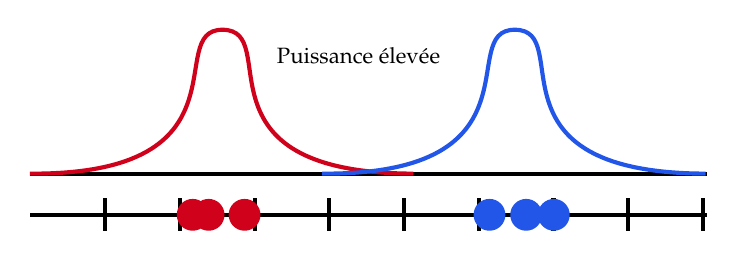
\begin{tikzpicture}[x=0.75pt,y=0.75pt,yscale=-1,xscale=1]
%uncomment if require: \path (0,176); %set diagram left start at 0, and has height of 176

%Straight Lines [id:da864976542619565] 
\draw [line width=1.5]    (245.5,117.83) -- (571.5,117.83) (281.5,109.83) -- (281.5,125.83)(317.5,109.83) -- (317.5,125.83)(353.5,109.83) -- (353.5,125.83)(389.5,109.83) -- (389.5,125.83)(425.5,109.83) -- (425.5,125.83)(461.5,109.83) -- (461.5,125.83)(497.5,109.83) -- (497.5,125.83)(533.5,109.83) -- (533.5,125.83)(569.5,109.83) -- (569.5,125.83) ;
%Straight Lines [id:da9295821978585093] 
\draw [line width=1.5]    (245.17,98) -- (571.5,98) ;
%Curve Lines [id:da28384300225010417] 
\draw [color={rgb, 255:red, 208; green, 2; blue, 27 }  ,draw opacity=1 ][line width=1.5]    (245.17,98) .. controls (353.67,98.67) and (309,28.67) .. (338,28.67) .. controls (368,28.67) and (320.67,97.67) .. (430,98) ;
%Curve Lines [id:da19190888762749303] 
\draw [color={rgb, 255:red, 33; green, 86; blue, 233 }  ,draw opacity=1 ][line width=1.5]    (386,98) .. controls (494.5,98.67) and (449.83,28.67) .. (478.83,28.67) .. controls (508.83,28.67) and (461.5,97.67) .. (570.83,98) ;
%Shape: Circle [id:dp23295532013997544] 
\draw  [draw opacity=0][fill={rgb, 255:red, 208; green, 2; blue, 27 }  ,fill opacity=1 ] (316,117.83) .. controls (316,113.6) and (319.43,110.17) .. (323.67,110.17) .. controls (327.9,110.17) and (331.33,113.6) .. (331.33,117.83) .. controls (331.33,122.07) and (327.9,125.5) .. (323.67,125.5) .. controls (319.43,125.5) and (316,122.07) .. (316,117.83) -- cycle ;
%Shape: Circle [id:dp6583442494748755] 
\draw  [draw opacity=0][fill={rgb, 255:red, 208; green, 2; blue, 27 }  ,fill opacity=1 ] (323.67,117.83) .. controls (323.67,113.6) and (327.1,110.17) .. (331.33,110.17) .. controls (335.57,110.17) and (339,113.6) .. (339,117.83) .. controls (339,122.07) and (335.57,125.5) .. (331.33,125.5) .. controls (327.1,125.5) and (323.67,122.07) .. (323.67,117.83) -- cycle ;
%Shape: Circle [id:dp7278683126625956] 
\draw  [draw opacity=0][fill={rgb, 255:red, 208; green, 2; blue, 27 }  ,fill opacity=1 ] (341,117.83) .. controls (341,113.6) and (344.43,110.17) .. (348.67,110.17) .. controls (352.9,110.17) and (356.33,113.6) .. (356.33,117.83) .. controls (356.33,122.07) and (352.9,125.5) .. (348.67,125.5) .. controls (344.43,125.5) and (341,122.07) .. (341,117.83) -- cycle ;
%Shape: Circle [id:dp6846096733160589] 
\draw  [draw opacity=0][fill={rgb, 255:red, 33; green, 86; blue, 233 }  ,fill opacity=1 ] (459,117.83) .. controls (459,113.6) and (462.43,110.17) .. (466.67,110.17) .. controls (470.9,110.17) and (474.33,113.6) .. (474.33,117.83) .. controls (474.33,122.07) and (470.9,125.5) .. (466.67,125.5) .. controls (462.43,125.5) and (459,122.07) .. (459,117.83) -- cycle ;
%Shape: Circle [id:dp05843938160550621] 
\draw  [draw opacity=0][fill={rgb, 255:red, 33; green, 86; blue, 233 }  ,fill opacity=1 ] (476.67,117.83) .. controls (476.67,113.6) and (480.1,110.17) .. (484.33,110.17) .. controls (488.57,110.17) and (492,113.6) .. (492,117.83) .. controls (492,122.07) and (488.57,125.5) .. (484.33,125.5) .. controls (480.1,125.5) and (476.67,122.07) .. (476.67,117.83) -- cycle ;
%Shape: Circle [id:dp2540684792866683] 
\draw  [draw opacity=0][fill={rgb, 255:red, 33; green, 86; blue, 233 }  ,fill opacity=1 ] (490,117.83) .. controls (490,113.6) and (493.43,110.17) .. (497.67,110.17) .. controls (501.9,110.17) and (505.33,113.6) .. (505.33,117.83) .. controls (505.33,122.07) and (501.9,125.5) .. (497.67,125.5) .. controls (493.43,125.5) and (490,122.07) .. (490,117.83) -- cycle ;

% Text Node
\draw (363,36) node [anchor=north west][inner sep=0.75pt]  [font=\footnotesize,color={rgb, 255:red, 255; green, 255; blue, 255 }  ,opacity=1 ] [align=left] {\textcolor{black}{Puissance élevée}};


\end{tikzpicture}
		\end{center}
		\begin{itemize}
		\item	 La probabilité de \textbf{correctement} rejeter l'hypothèse nulle (que les deux échantillons proviennent d'une même distribution) est élevée;
		\item	On peut aussi dire qu'il y a une forte probabilité de \textbf{correctement} obtenir une faible valeur $p$.
		\end{itemize}
	\item	Se \textbf{chevauchent}, la puissance sera \textbf{faible}:
		\begin{center}
		\tikzset{every picture/.style={line width=0.75pt}} %set default line width to 0.75pt        

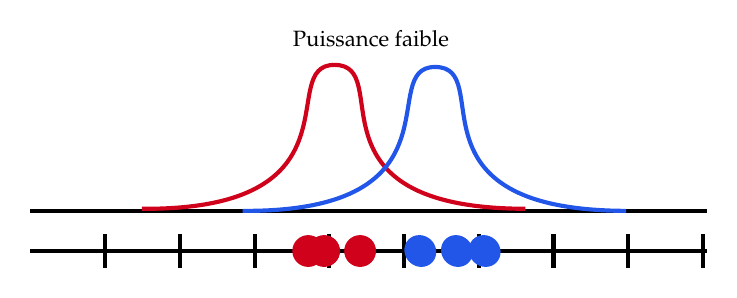
\begin{tikzpicture}[x=0.75pt,y=0.75pt,yscale=-1,xscale=1]
%uncomment if require: \path (0,176); %set diagram left start at 0, and has height of 176

%Straight Lines [id:da674545395459474] 
\draw [line width=1.5]    (244.83,117.33) -- (570.83,117.33) (280.83,109.33) -- (280.83,125.33)(316.83,109.33) -- (316.83,125.33)(352.83,109.33) -- (352.83,125.33)(388.83,109.33) -- (388.83,125.33)(424.83,109.33) -- (424.83,125.33)(460.83,109.33) -- (460.83,125.33)(496.83,109.33) -- (496.83,125.33)(532.83,109.33) -- (532.83,125.33)(568.83,109.33) -- (568.83,125.33) ;
%Shape: Circle [id:dp5899062048279418] 
\draw  [draw opacity=0][fill={rgb, 255:red, 208; green, 2; blue, 27 }  ,fill opacity=1 ] (371,117.33) .. controls (371,113.1) and (374.43,109.67) .. (378.67,109.67) .. controls (382.9,109.67) and (386.33,113.1) .. (386.33,117.33) .. controls (386.33,121.57) and (382.9,125) .. (378.67,125) .. controls (374.43,125) and (371,121.57) .. (371,117.33) -- cycle ;
%Shape: Circle [id:dp033764139219446765] 
\draw  [draw opacity=0][fill={rgb, 255:red, 208; green, 2; blue, 27 }  ,fill opacity=1 ] (378.67,117.33) .. controls (378.67,113.1) and (382.1,109.67) .. (386.33,109.67) .. controls (390.57,109.67) and (394,113.1) .. (394,117.33) .. controls (394,121.57) and (390.57,125) .. (386.33,125) .. controls (382.1,125) and (378.67,121.57) .. (378.67,117.33) -- cycle ;
%Shape: Circle [id:dp9956436610120569] 
\draw  [draw opacity=0][fill={rgb, 255:red, 208; green, 2; blue, 27 }  ,fill opacity=1 ] (396,117.33) .. controls (396,113.1) and (399.43,109.67) .. (403.67,109.67) .. controls (407.9,109.67) and (411.33,113.1) .. (411.33,117.33) .. controls (411.33,121.57) and (407.9,125) .. (403.67,125) .. controls (399.43,125) and (396,121.57) .. (396,117.33) -- cycle ;
%Straight Lines [id:da9463171904376761] 
\draw [line width=1.5]    (244.5,98) -- (570.83,98) ;
%Curve Lines [id:da7529446506143549] 
\draw [color={rgb, 255:red, 208; green, 2; blue, 27 }  ,draw opacity=1 ][line width=1.5]    (298.5,97) .. controls (407,97.67) and (362.33,27.67) .. (391.33,27.67) .. controls (421.33,27.67) and (374,96.67) .. (483.33,97) ;
%Curve Lines [id:da7479872172646262] 
\draw [color={rgb, 255:red, 33; green, 86; blue, 233 }  ,draw opacity=1 ][line width=1.5]    (347,98) .. controls (455.5,98.67) and (410.83,28.67) .. (439.83,28.67) .. controls (469.83,28.67) and (422.5,97.67) .. (531.83,98) ;
%Shape: Circle [id:dp8825558203269679] 
\draw  [draw opacity=0][fill={rgb, 255:red, 33; green, 86; blue, 233 }  ,fill opacity=1 ] (425,117.33) .. controls (424.72,113.1) and (427.93,109.67) .. (432.17,109.67) .. controls (436.4,109.67) and (440.06,113.1) .. (440.33,117.33) .. controls (440.61,121.57) and (437.4,125) .. (433.17,125) .. controls (428.93,125) and (425.28,121.57) .. (425,117.33) -- cycle ;
%Shape: Circle [id:dp2808249488586654] 
\draw  [draw opacity=0][fill={rgb, 255:red, 33; green, 86; blue, 233 }  ,fill opacity=1 ] (442.67,117.33) .. controls (442.39,113.1) and (445.6,109.67) .. (449.83,109.67) .. controls (454.07,109.67) and (457.72,113.1) .. (458,117.33) .. controls (458.28,121.57) and (455.07,125) .. (450.83,125) .. controls (446.6,125) and (442.94,121.57) .. (442.67,117.33) -- cycle ;
%Shape: Circle [id:dp8643138982751464] 
\draw  [draw opacity=0][fill={rgb, 255:red, 33; green, 86; blue, 233 }  ,fill opacity=1 ] (456,117.33) .. controls (455.72,113.1) and (458.93,109.67) .. (463.17,109.67) .. controls (467.4,109.67) and (471.06,113.1) .. (471.33,117.33) .. controls (471.61,121.57) and (468.4,125) .. (464.17,125) .. controls (459.93,125) and (456.28,121.57) .. (456,117.33) -- cycle ;

% Text Node
\draw (370,10) node [anchor=north west][inner sep=0.75pt]  [font=\footnotesize,color={rgb, 255:red, 255; green, 255; blue, 255 }  ,opacity=1 ] [align=left] {\textcolor{black}{Puissance faible}};


\end{tikzpicture}
		\end{center}
		\begin{itemize}
		\item	 La probabilité \textbf{d’incorrectement} rejeter l'hypothèse nulle (que les deux échantillons proviennent d'une même distribution) est élevée;
		\item	On peut aussi dire qu'il y a une forte probabilité \textbf{d’incorrectement} obtenir une faible valeur $p$;
		\item	Cependant, la puissance peut être augmentée avec plus d'observations.
		\end{itemize}
\end{itemize}
\end{definitionNOHFILLsub}

\begin{definitionNOHFILLsub}[La variabilité des données]
Si la variabilité de la distribution est
\begin{itemize}
	\item	\textbf{Faible}, alors la variabilité de l'échantillon sera probablement faible aussi menant à une puissance très \textbf{élevée}:
		\begin{center}
		\tikzset{every picture/.style={line width=0.75pt}} %set default line width to 0.75pt        

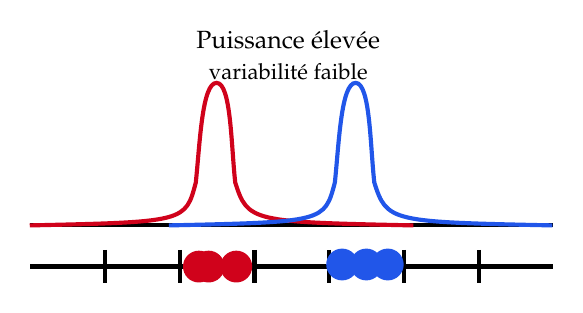
\begin{tikzpicture}[x=0.75pt,y=0.75pt,yscale=-1,xscale=1]
%uncomment if require: \path (0,176); %set diagram left start at 0, and has height of 176

%Straight Lines [id:da864976542619565] 
\draw [line width=1.5]    (245.42,117.83) -- (497.17,117.83) (281.42,109.83) -- (281.42,125.83)(317.42,109.83) -- (317.42,125.83)(353.42,109.83) -- (353.42,125.83)(389.42,109.83) -- (389.42,125.83)(425.42,109.83) -- (425.42,125.83)(461.42,109.83) -- (461.42,125.83) ;
%Straight Lines [id:da9295821978585093] 
\draw [line width=1.5]    (245.17,98) -- (497.17,98) ;
%Shape: Circle [id:dp23295532013997544] 
\draw  [draw opacity=0][fill={rgb, 255:red, 208; green, 2; blue, 27 }  ,fill opacity=1 ] (319,117.83) .. controls (319,113.6) and (322.43,110.17) .. (326.67,110.17) .. controls (330.9,110.17) and (334.33,113.6) .. (334.33,117.83) .. controls (334.33,122.07) and (330.9,125.5) .. (326.67,125.5) .. controls (322.43,125.5) and (319,122.07) .. (319,117.83) -- cycle ;
%Shape: Circle [id:dp6583442494748755] 
\draw  [draw opacity=0][fill={rgb, 255:red, 208; green, 2; blue, 27 }  ,fill opacity=1 ] (323.67,117.83) .. controls (323.67,113.6) and (327.1,110.17) .. (331.33,110.17) .. controls (335.57,110.17) and (339,113.6) .. (339,117.83) .. controls (339,122.07) and (335.57,125.5) .. (331.33,125.5) .. controls (327.1,125.5) and (323.67,122.07) .. (323.67,117.83) -- cycle ;
%Shape: Circle [id:dp7278683126625956] 
\draw  [draw opacity=0][fill={rgb, 255:red, 208; green, 2; blue, 27 }  ,fill opacity=1 ] (337,117.83) .. controls (337,113.6) and (340.43,110.17) .. (344.67,110.17) .. controls (348.9,110.17) and (352.33,113.6) .. (352.33,117.83) .. controls (352.33,122.07) and (348.9,125.5) .. (344.67,125.5) .. controls (340.43,125.5) and (337,122.07) .. (337,117.83) -- cycle ;
%Shape: Circle [id:dp6846096733160589] 
\draw  [draw opacity=0][fill={rgb, 255:red, 33; green, 86; blue, 233 }  ,fill opacity=1 ] (388,116.83) .. controls (388,112.6) and (391.43,109.17) .. (395.67,109.17) .. controls (399.9,109.17) and (403.33,112.6) .. (403.33,116.83) .. controls (403.33,121.07) and (399.9,124.5) .. (395.67,124.5) .. controls (391.43,124.5) and (388,121.07) .. (388,116.83) -- cycle ;
%Shape: Circle [id:dp05843938160550621] 
\draw  [draw opacity=0][fill={rgb, 255:red, 33; green, 86; blue, 233 }  ,fill opacity=1 ] (399.67,116.83) .. controls (399.67,112.6) and (403.1,109.17) .. (407.33,109.17) .. controls (411.57,109.17) and (415,112.6) .. (415,116.83) .. controls (415,121.07) and (411.57,124.5) .. (407.33,124.5) .. controls (403.1,124.5) and (399.67,121.07) .. (399.67,116.83) -- cycle ;
%Shape: Circle [id:dp2540684792866683] 
\draw  [draw opacity=0][fill={rgb, 255:red, 33; green, 86; blue, 233 }  ,fill opacity=1 ] (410,116.83) .. controls (410,112.6) and (413.43,109.17) .. (417.67,109.17) .. controls (421.9,109.17) and (425.33,112.6) .. (425.33,116.83) .. controls (425.33,121.07) and (421.9,124.5) .. (417.67,124.5) .. controls (413.43,124.5) and (410,121.07) .. (410,116.83) -- cycle ;
%Curve Lines [id:da9834393207352259] 
\draw [color={rgb, 255:red, 208; green, 2; blue, 27 }  ,draw opacity=1 ][line width=1.5]    (245.17,98) .. controls (320.17,96.33) and (320.17,96.33) .. (325.17,77.33) .. controls (327.17,58.33) and (328.17,29.33) .. (335.17,29.33) .. controls (342.17,29.33) and (342.17,59.33) .. (344.17,77.33) .. controls (350.17,96.33) and (352.17,96.33) .. (430,98) ;
%Curve Lines [id:da5775597107131041] 
\draw [color={rgb, 255:red, 33; green, 86; blue, 233 }  ,draw opacity=1 ][line width=1.5]    (312.17,98) .. controls (387.17,96.33) and (387.17,96.33) .. (392.17,77.33) .. controls (394.17,58.33) and (395.17,29.33) .. (402.17,29.33) .. controls (409.17,29.33) and (409.17,59.33) .. (411.17,77.33) .. controls (417.17,96.33) and (419.17,96.33) .. (497,98) ;

% Text Node
\draw (324,3) node [anchor=north west][inner sep=0.75pt]  [font=\small,color={rgb, 255:red, 0; green, 0; blue, 0 }  ,opacity=1 ] [align=left] {\begin{minipage}[lt]{66.6825pt}\setlength\topsep{0pt}
\begin{center}
Puissance élevée\\{\footnotesize variabilité faible}
\end{center}

\end{minipage}};


\end{tikzpicture}
		\end{center}
	\item	\textbf{Élevée}, alors la variabilité de l'échantillon sera probablement élevée aussi menant à une puissance \textbf{faible}: 
		\begin{center}
		\tikzset{every picture/.style={line width=0.75pt}} %set default line width to 0.75pt        

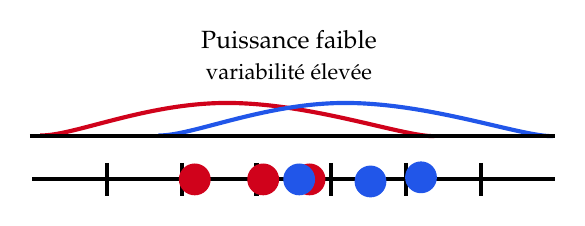
\begin{tikzpicture}[x=0.75pt,y=0.75pt,yscale=-1,xscale=1]
%uncomment if require: \path (0,176); %set diagram left start at 0, and has height of 176

%Straight Lines [id:da224342647816256] 
\draw [line width=1.5]    (291.42,122.83) -- (543.17,122.83) (327.42,114.83) -- (327.42,130.83)(363.42,114.83) -- (363.42,130.83)(399.42,114.83) -- (399.42,130.83)(435.42,114.83) -- (435.42,130.83)(471.42,114.83) -- (471.42,130.83)(507.42,114.83) -- (507.42,130.83) ;
%Shape: Circle [id:dp7289237376471596] 
\draw  [draw opacity=0][fill={rgb, 255:red, 208; green, 2; blue, 27 }  ,fill opacity=1 ] (362,122.83) .. controls (362,118.6) and (365.43,115.17) .. (369.67,115.17) .. controls (373.9,115.17) and (377.33,118.6) .. (377.33,122.83) .. controls (377.33,127.07) and (373.9,130.5) .. (369.67,130.5) .. controls (365.43,130.5) and (362,127.07) .. (362,122.83) -- cycle ;
%Shape: Circle [id:dp6581028616853248] 
\draw  [draw opacity=0][fill={rgb, 255:red, 208; green, 2; blue, 27 }  ,fill opacity=1 ] (417.3,122.83) .. controls (417.3,118.6) and (420.73,115.17) .. (424.96,115.17) .. controls (429.2,115.17) and (432.63,118.6) .. (432.63,122.83) .. controls (432.63,127.07) and (429.2,130.5) .. (424.96,130.5) .. controls (420.73,130.5) and (417.3,127.07) .. (417.3,122.83) -- cycle ;
%Shape: Circle [id:dp32832339728857773] 
\draw  [draw opacity=0][fill={rgb, 255:red, 208; green, 2; blue, 27 }  ,fill opacity=1 ] (394.96,122.83) .. controls (394.96,118.6) and (398.39,115.17) .. (402.63,115.17) .. controls (406.86,115.17) and (410.3,118.6) .. (410.3,122.83) .. controls (410.3,127.07) and (406.86,130.5) .. (402.63,130.5) .. controls (398.39,130.5) and (394.96,127.07) .. (394.96,122.83) -- cycle ;
%Shape: Circle [id:dp8463878803176157] 
\draw  [draw opacity=0][fill={rgb, 255:red, 33; green, 86; blue, 233 }  ,fill opacity=1 ] (412.3,122.83) .. controls (412.3,118.6) and (415.73,115.17) .. (419.96,115.17) .. controls (424.2,115.17) and (427.63,118.6) .. (427.63,122.83) .. controls (427.63,127.07) and (424.2,130.5) .. (419.96,130.5) .. controls (415.73,130.5) and (412.3,127.07) .. (412.3,122.83) -- cycle ;
%Shape: Circle [id:dp41576741952688256] 
\draw  [draw opacity=0][fill={rgb, 255:red, 33; green, 86; blue, 233 }  ,fill opacity=1 ] (446.67,123.83) .. controls (446.67,119.6) and (450.1,116.17) .. (454.33,116.17) .. controls (458.57,116.17) and (462,119.6) .. (462,123.83) .. controls (462,128.07) and (458.57,131.5) .. (454.33,131.5) .. controls (450.1,131.5) and (446.67,128.07) .. (446.67,123.83) -- cycle ;
%Shape: Circle [id:dp7322447345202854] 
\draw  [draw opacity=0][fill={rgb, 255:red, 33; green, 86; blue, 233 }  ,fill opacity=1 ] (471,121.83) .. controls (471,117.6) and (474.43,114.17) .. (478.67,114.17) .. controls (482.9,114.17) and (486.33,117.6) .. (486.33,121.83) .. controls (486.33,126.07) and (482.9,129.5) .. (478.67,129.5) .. controls (474.43,129.5) and (471,126.07) .. (471,121.83) -- cycle ;
%Curve Lines [id:da3201541308920388] 
\draw [color={rgb, 255:red, 208; green, 2; blue, 27 }  ,draw opacity=1 ][line width=1.5]    (295.17,101.67) .. controls (311.17,102) and (346.17,86) .. (385.17,86) .. controls (426.17,86) and (470.33,102.33) .. (485.17,102) ;
%Curve Lines [id:da0520324915772159] 
\draw [color={rgb, 255:red, 33; green, 86; blue, 233 }  ,draw opacity=1 ][line width=1.5]    (352.17,101.67) .. controls (368.17,102) and (403.17,86) .. (442.17,86) .. controls (483.17,86) and (527.33,102.33) .. (542.17,102) ;
%Straight Lines [id:da9874290431386423] 
\draw [line width=1.5]    (290.17,102) -- (543.17,102) ;

% Text Node
\draw (371,50) node [anchor=north west][inner sep=0.75pt]  [font=\small,color={rgb, 255:red, 0; green, 0; blue, 0 }  ,opacity=1 ] [align=left] {\begin{minipage}[lt]{64.149144pt}\setlength\topsep{0pt}
\begin{center}
Puissance faible\\{\footnotesize variabilité élevée}
\end{center}

\end{minipage}};
\end{tikzpicture}
		\end{center}
\end{itemize}
\end{definitionNOHFILLsub}

Il existe plusieurs mesures qui permettent de considérer la variabilité des données ainsi que la forme de la distribution. Entres autre, il y a le \og \textit{\textbf{effect size ($d$)}} \fg{} où \lfbox[formula]{$d	=	\frac{\bar{x} - \bar{y}}{s^{2}_{p}}$}.

\begin{definitionNOHFILLsub}[La taille de l'échantillon de données]
Un grand échantillon de données peut compenser pour des distributions qui se chevauchent ou une variabilité élevée. Ça permet d'augmenter notre \textit{confiance} qu'il y a bel et bien une différence entre les échantillons. \\

En contraste, nous n'avons pas besoin d'un grand échantillon de données pour des distributions très distinctes ou avec une faible variabilité; nous sommes déjà confiants que les distributions sont différentes.
\end{definitionNOHFILLsub}

\begin{definitionNOHFILLsub}[Le test statistique]
Certains tests ont une puissance plus élevée que les autres. \\
Cela dit, le test $t$ habituel est très puissant.
\end{definitionNOHFILLsub}

\subsubsection{La fonction de puissance}

La fonction de puissance est \lfbox[formula]{$\gamma(\theta)	=	\Pr\left\{(X_{1}, \dots, X_{n}) \in \mathcal{C} ; \theta \right\}$} ; c'est-à-dire, la probabilité de rejeter l'hypothèse nulle $\mathrm{H}_{0}$ si la \textbf{vraie} valeur du paramètre est $\theta \in \Theta$. 
\begin{itemize}
	\item	C'est une fonction de $\theta$ ;
	\item	Idéalement, si l'hypothèse nulle est :
		\begin{description}
		\item[acceptée]	on souhaite que $\gamma(\theta)	=	0$ puisque $\theta \in \Theta_{0}$.
			\begin{itemize}
			\item	On dénote $\gamma(\theta_{0})	=	\Pr\left\{(X_{1}, \dots, X_{n}) \in \mathcal{C} ;  \theta \in \Theta_{0}\right\}	=	0$.
			\end{itemize}
		\item[rejetée]	on souhaite que $\gamma(\theta)	=	1$ puisque $\theta \in \Theta_{1}$.
			\begin{itemize}
			\item	On dénote $\gamma(\theta_{1})	=	\Pr\left\{(X_{1}, \dots, X_{n}) \in \mathcal{C} ; \theta \in \Theta_{1}\right\}	=	1$.
			\end{itemize}
		\end{description}
\end{itemize}

Si, par exemple, on rejette l'hypothèse nulle, on pourrait tracer la fonction de puissance pour toutes les valeurs possibles de l'ensemble $\Theta_{1}$.


%%	
%	\lfbox[formula]{$n \geq \left(\frac{z}{k - \mu_{1}}\right)^{2}\sigma^{2}$}.


\columnbreak

\subsection{Tests optimaux}
\begin{distributions}[Notation]
\begin{description}
	\item[$\delta$]	(Procédure de) test ;
	\item[$\alpha(\delta)$]	Probabilité d'une erreur de type I pour un test $\delta$ ;
		\begin{itemize}
		\item	$\alpha(\delta)	=	\Pr\left\{(X_{1}, \dots, X_{n}) \in \mathcal{C} ;  \theta \in \Theta_{0}\right\}	=	\gamma(\theta_{0})$.
		\end{itemize}
	\item[$\beta(\delta)$]	Probabilité d'une erreur de type II pour un test $\delta$ ;
		\begin{itemize}
		\item	$\beta(\delta)	=	\Pr\left\{(X_{1}, \dots, X_{n}) \in \mathcal{C}^{\complement} ;  \theta \in \Theta_{1}\right\}	=	1 - \gamma(\theta_{1})$.
		\end{itemize}
\end{description}

\end{distributions}
Pour mettre en contexte cette notation, revoici le tableau des types d'erreurs pour un test $\delta$ :
\begin{center}
\tikzset{every picture/.style={line width=0.75pt}} %set default line width to 0.75pt        

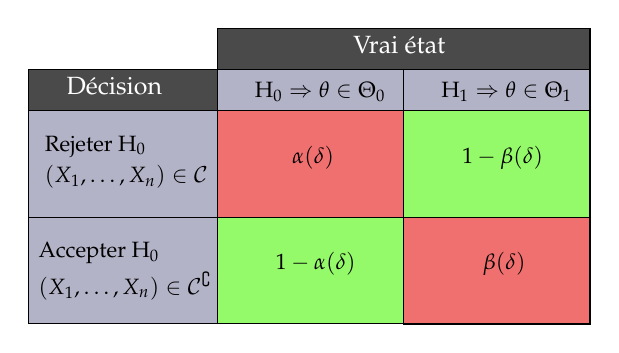
\begin{tikzpicture}[x=0.75pt,y=0.75pt,yscale=-1,xscale=1]
%uncomment if require: \path (0,165); %set diagram left start at 0, and has height of 165

%Shape: Rectangle [id:dp5658804967739193] 
\draw  [fill={rgb, 255:red, 240; green, 111; blue, 111 }  ,fill opacity=1 ] (74,50.17) -- (163.83,50.17) -- (163.83,101.5) -- (74,101.5) -- cycle ;
%Shape: Rectangle [id:dp933461228347003] 
\draw  [fill={rgb, 255:red, 240; green, 111; blue, 111 }  ,fill opacity=1 ] (163.83,101.5) -- (253.67,101.5) -- (253.67,152.83) -- (163.83,152.83) -- cycle ;
%Shape: Rectangle [id:dp24194313951746427] 
\draw  [fill={rgb, 255:red, 148; green, 250; blue, 106 }  ,fill opacity=1 ] (163.83,50) -- (253.67,50) -- (253.67,101.33) -- (163.83,101.33) -- cycle ;
%Shape: Rectangle [id:dp27324261874552724] 
\draw  [fill={rgb, 255:red, 148; green, 250; blue, 106 }  ,fill opacity=1 ] (74,101.33) -- (163.83,101.33) -- (163.83,152.67) -- (74,152.67) -- cycle ;

%Shape: Rectangle [id:dp9425087952138109] 
\draw  [fill={rgb, 255:red, 179; green, 179; blue, 200 }  ,fill opacity=1 ] (74,30.17) -- (163.83,30.17) -- (163.83,50) -- (74,50) -- cycle ;
%Shape: Rectangle [id:dp4099498200973881] 
\draw  [fill={rgb, 255:red, 179; green, 179; blue, 200 }  ,fill opacity=1 ] (163.83,30.17) -- (253.67,30.17) -- (253.67,50) -- (163.83,50) -- cycle ;
%Shape: Rectangle [id:dp35293578825776084] 
\draw  [fill={rgb, 255:red, 179; green, 179; blue, 200 }  ,fill opacity=1 ] (-17,101.33) -- (74,101.33) -- (74,152.67) -- (-17,152.67) -- cycle ;
%Shape: Rectangle [id:dp2841127241620307] 
\draw  [fill={rgb, 255:red, 179; green, 179; blue, 200 }  ,fill opacity=1 ] (-17,50.17) -- (74,50.17) -- (74,101.5) -- (-17,101.5) -- cycle ;

%Shape: Rectangle [id:dp40513736937576916] 
\draw  [fill={rgb, 255:red, 74; green, 74; blue, 74 }  ,fill opacity=1 ] (74,10.33) -- (253.67,10.33) -- (253.67,30.17) -- (74,30.17) -- cycle ;
%Shape: Rectangle [id:dp5918283025493905] 
\draw  [fill={rgb, 255:red, 74; green, 74; blue, 74 }  ,fill opacity=1 ] (-17,30.33) -- (74,30.33) -- (74,50.17) -- (-17,50.17) -- cycle ;

% Text Node
\draw (138.33,13) node [anchor=north west][inner sep=0.75pt]  [font=\small,color={rgb, 255:red, 255; green, 255; blue, 255 }  ,opacity=1 ] [align=left] {Vrai état};
% Text Node
\draw (90.92,35) node [anchor=north west][inner sep=0.75pt]  [font=\footnotesize,color={rgb, 255:red, 0; green, 0; blue, 0 }  ,opacity=1 ] [align=left] {$ \text{H}_{0} \Rightarrow \theta \in \Theta_{0}$};
% Text Node
\draw (180.75,35) node [anchor=north west][inner sep=0.75pt]  [font=\footnotesize,color={rgb, 255:red, 0; green, 0; blue, 0 }  ,opacity=1 ] [align=left] {$ \text{H}_{1} \Rightarrow \theta \in \Theta_{1}$};

% Text Node
\draw (-13.25,112) node [anchor=north west][inner sep=0.75pt]  [font=\footnotesize,color={rgb, 255:red, 0; green, 0; blue, 0 }  ,opacity=1 ] [align=left] {\shortstack[l]{Accepter $\text{H}_{0}$\\ $(X_{1}, \dots, X_{n}) \in \mathcal{C}^{\complement}$ }};
% Text Node
\draw (-10.25,60.83) node [anchor=north west][inner sep=0.75pt]  [font=\footnotesize,color={rgb, 255:red, 0; green, 0; blue, 0 }  ,opacity=1] [align=left] {\shortstack[l]{Rejeter $\text{H}_{0}$\\ $(X_{1}, \dots, X_{n}) \in \mathcal{C}$}};

% Text Node
\draw (0.25,32.75) node [anchor=north west][inner sep=0.75pt]  [font=\small,color={rgb, 255:red, 255; green, 255; blue, 255 }  ,opacity=1 ] [align=left] {Décision};
% Text Node
\draw (108.92,65.83) node [anchor=north west][inner sep=0.75pt]  [font=\footnotesize,color={rgb, 255:red, 0; green, 0; blue, 0 }  ,opacity=1 ] [align=left] 
{$\alpha(\delta)$};
% Text Node
\draw (200.75,117) node [anchor=north west][inner sep=0.75pt]  [font=\footnotesize,color={rgb, 255:red, 0; green, 0; blue, 0 }  ,opacity=1 ] [align=left] {$\beta(\delta)$};
% Text Node
\draw (100.92,117) node [anchor=north west][inner sep=0.75pt]  [font=\footnotesize,color={rgb, 255:red, 0; green, 0; blue, 0 }  ,opacity=1 ] [align=left] {$1 - \alpha(\delta)$};
% Text Node
\draw (190.75,65.67) node [anchor=north west][inner sep=0.75pt]  [font=\footnotesize,color={rgb, 255:red, 0; green, 0; blue, 0 }  ,opacity=1 ] [align=left] {$1 - \beta(\delta)$};
\end{tikzpicture}
\end{center}

\begin{itemize}
	\item	\textit{En théorie}, on minimise la probabilité d'une erreur de type I \textbf{et} de II ; 
	\item	\textit{En réalité}, il y a un compromis et on ne pourra pas avoir des très petites probabilités pour les deux ;
	\item	Le contexte va déterminer ce qu'on souhaite minimiser le plus ;
		\begin{itemize}
		\item	Par exemple, soit l'hypothèse nulle que quelqu'un n'a pas le cancer ;
		\item	Il est plus grave de dire à quelqu'un qu'il n'a pas le cancer alors qu'il l'a (erreur de type II) que de dire qu'il a le cancer alors qu'il ne l'a pas (erreur de type I) ;
		\item	Dans ce contexte, on souhaiterait minimiser l'erreur de type II $\beta(\delta)$ plus que celle de type I $\alpha(\delta)$.
		\end{itemize}
%	\item	Cela dit, on peut tenter de minimiser une \textit{fonction} des deux erreurs.
\end{itemize}

Puisqu'il est impossible de trouver un test $\delta$ pour lequel les probabilités d'erreurs de type I et II sont très petites, on :
\begin{enumerate}
	\item	Fixe l'erreur de type I à un seuil, alias une taille de région critique, $k$.
	\item	Trouve parmi tous les sous-ensembles de taille $k$ celui qui minimise l'erreur de type II.
\end{enumerate}

\begin{definitionNOHFILLprop}[Tests optimaux]
%Puisqu'il est impossible de trouver un test $\delta$ pour lequel les probabilités d'erreurs de type I et II sont très petites, on peut minimiser la fonction \lfbox[formula]{$a\alpha(\delta) + b\beta(\delta)$} des \lfbox[conditions]{constantes $a, b > 0$}.\\

%\tcbline

Soit un test $\delta^{*}$ avec les hypothèses \hyperlink{hyp-simple}{\color{blue!80!white}\underline{simples}} :
\begin{align*}
	\mathrm{H}_{0}	&:	\theta	=	\theta_{0}	\\
	\mathrm{H}_{1}	&:	\theta	=	\theta_{1}
\end{align*}
\begin{itemize}
	\item	Par exemple, on pourrait avoir une distribution Bernoulli et poser $\mathrm{H}_{0}	:	p	=	0.4$ v.s. $\mathrm{H}_{1}	:	p	=	0.6$.
\end{itemize}
\

La procédure pour trouver la région critique $\mathcal{C}$ optimale de taille $\alpha$ du test $\delta^{\ast}$ est la suivante :
\begin{enumerate}
	\item	On trouve une région critique (alias, un sous-ensemble de $\mathcal{S}$) $\mathcal{C}$ tel que la probabilité $\alpha(\delta^{\ast})$ d'une erreur de type I est de $\alpha$.
		\begin{itemize}
		\item	C'est-à-dire, \lfbox[conditions]{$\alpha(\delta^{\ast})	=	Pr\left\{(X_{1}, \dots, X_{n}) \in \mathcal{C} ;  \theta	=	\theta_{0}\right\}	=	\alpha$}.
		\item	Cependant, ce critère n'identifie par un sous-ensemble unique ;
		\item	Il y a une multitude de sous-ensembles $\mathcal{A}$ de $\mathcal{S}$ dont la probabilité que l'échantillon aléatoire y soit contenu (sous l'hypothèse nulle) est aussi $\alpha$ ;
		\item	C'est-à-dire, $Pr\left\{(X_{1}, \dots, X_{n}) \in \mathcal{A}; \theta	=	\theta_{0}	\right\}	=	\alpha$.
		\end{itemize}
	\item	On pose que la probabilité que l'échantillon aléatoire soit dans la région critique $\mathcal{C}$ (sous l'hypothèse alternative) est supérieure à la probabilité que l'échantillon aléatoire soit contenu dans tout autre sous-ensemble $\mathcal{A}$.
		\begin{itemize}
		\item	C'est-à-dire, \lfbox[formula]{$Pr\left\{(X_{1}, \dots, X_{n}) \in \mathcal{C}; \theta	=	\theta_{1}	\right\}	\geq Pr\big\{(X_{1}, \dots, X_{n}) \in \mathcal{A};$} \lfbox[formula]{$\theta	=	\theta_{1}	\big\}$}.
		\end{itemize}
\end{enumerate}

Avec ces deux critères, on trouve \textit{\textbf{la}} région critique $\mathcal{C}$ de taille $\alpha$ \textbf{optimale} pour tester les hypothèses simples.

%%%%	%%%%	%%%%	%%%%	%%%%	%%%%	%%%%	%%%%	%%%%	%%%%	%%%%	
%%%	Test optimal selon les NDC de M.-P.	%%%%	
%\begin{itemize}
%	\item	 $\mathrm{H}_{0}$ est acceptée si \lfbox[conditions]{$af(\bm{x} ; \theta_{0})	>	bf(\bm{x} ; \theta_{1})$} ;
%	\item	 $\mathrm{H}_{0}$ est rejetée si \lfbox[conditions]{$af(\bm{x} ; \theta_{0})	<	bf(\bm{x} ; \theta_{1})$} ;
%	\item	Si \lfbox[conditions]{$af(\bm{x} ; \theta_{0})	=	bf(\bm{x} ; \theta_{1})$} soit $\mathrm{H}_{0}$ ou $\mathrm{H}_{1}$ peut être acceptée.
%\end{itemize}
%
%Pour tout autre test $\delta$, \lfbox[formula]{$a\alpha(\delta^{*}) + b\beta(\delta^{*})	\leq	a\alpha(\delta) + b\beta(\delta)$}.
%%%%	%%%%	%%%%	%%%%	%%%%	%%%%	%%%%	%%%%	%%%%	%%%%	%%%%	
\end{definitionNOHFILLprop}

En bref, on pose fixe à un seuil $\alpha$ la fonction de puissance posant que le vrai paramètre $\theta	=	\theta_{0}$ puis on trouve la région critique qui maximise la puissance posant que le vrai paramètre $\theta	=	\theta_{1}$.

\begin{formula}{Exemple avec une distribution binomiale}
Soit :
\begin{itemize}
	\item	La variable aléatoire $X \sim Binom(n = 3, p = \theta)$.
		\begin{itemize}
		\item	Alors, $\mathcal{S}	=	\{x : x	=	0, 1, 2, 3\}$.
		\end{itemize}
	\item	Les hypothèses : \\
		\begin{align*}
		\mathrm{H}_{0}	&:	\theta	=	0.50	\\
		\mathrm{H}_{1}	&:	\theta	=	0.75
		\end{align*}
	\item	Le seuil de signifiance $\alpha	=	0.125$.
	\item	Les sous-ensembles $\mathcal{A}_{1}	=	\{x : x = 0\}$ et $\mathcal{A}_{2}	=	\{x : x = 3\}$ de $\mathcal{S}$.
\end{itemize}
Alors, $\Pr( X \in \mathcal{A}_{1}; \theta	=	0.50)	=	\Pr( X \in \mathcal{A}_{2}; \theta	=	0.50)	=	0.125$ et il n'y a pas d'autres sous-ensembles de $\mathcal{S}$ avec la même taille de $0.125$.\\
Il s'ensuit que soit $\mathcal{A}_{1}$ ou $\mathcal{A}_{2}$ est la région critique $\mathcal{C}$ optimale de taille $\alpha$ pour tester $\mathrm{H}_{0}$ contre $\mathrm{H}_{1}$.\\

On trouve que $\Pr( X \in \mathcal{A}_{1}; \theta	=	0.75)	=	0.015625$ alors que $\Pr( X \in \mathcal{A}_{2}; \theta	=	0.75)	=	0.421875$. 
\begin{itemize}
	\item	Dans le premier cas :\\
		\setlength{\mathindent}{-1cm}
		\begin{align*}
		\Pr( \underbrace{X \in \mathcal{A}_{1}; \theta	=	0.75}_{\mathclap{\shortstack{rejeter $\mathrm{H}_{0}$ alors que $\mathrm{H}_{0}$\\ est faux ($\theta = 0.75$)}}})	
		&=	0.015625		&
		&<	&
		\Pr( \underbrace{X \in \mathcal{A}_{1}; \theta	=	0.50}_{\mathclap{\shortstack{rejeter $\mathrm{H}_{0}$ alors que $\mathrm{H}_{0}$\\ est vraie ($\theta = 0.50$)}}})	
		&=	0.125	
		\end{align*}
		\setlength{\mathindent}{1cm}
	\item	Dans le deuxième cas :\\
		\setlength{\mathindent}{-1cm}
		\begin{align*}
		\Pr( \underbrace{X \in \mathcal{A}_{2}; \theta	=	0.75}_{\mathclap{\shortstack{rejeter $\mathrm{H}_{0}$ alors que $\mathrm{H}_{0}$\\ est faux ($\theta = 0.75$)}}})	
		&=	0.421875		&
		&>	&
		\Pr( \underbrace{X \in \mathcal{A}_{2}; \theta	=	0.50}_{\mathclap{\shortstack{rejeter $\mathrm{H}_{0}$ alors que $\mathrm{H}_{0}$\\ est vraie ($\theta = 0.50$)}}})	
		&=	0.125	
		\end{align*}
		\setlength{\mathindent}{1cm}
	\item	Le premier sous-ensemble $\mathcal{A}_{1}$ n'est pas désirable, car on serait plus probable de incorrectement rejeter $\mathrm{H}_{0}$ lorsqu'elle est vraie (erreur de type I) que de correctement la rejeter lorsqu'elle est fausse ! 
	\item	Alors, on choisit $\mathcal{C}	=	\mathcal{A}_{2}	=	\{x: x = 3\}$.
\end{itemize}

D'ailleurs, la région est choisie en incluant dans $\mathcal{C}$ les points $x$ pour lesquels $f(x; \theta	=	0.50)$ est petite par rapport à $f(x; \theta	=	0.75)$.
\begin{itemize}
	\item	On peut d'ailleurs observer que le ratio $\frac{f(x; \theta	=	0.50)}{f(x; \theta	=	0.75)}$ évalué à $x	=	5$ est un minimum.
\end{itemize}
\end{formula}

On peut utiliser ce ratio comme outil pour identifier la région critique $\mathcal{C}$ optimale pour un seuil fixe de $\alpha$.


\columnbreak
\subsubsection{Cas d'hypothèses simples}

\begin{definitionNOHFILL}[Théorème de Neymann-Pearson]
%Le lemme de Neyman-Pearson trouve le test $\delta$ qui minimise la probabilité d'une erreur de type II $\beta(\delta)$ parmi tous les test dont la probabilité d'une erreur de type I $\alpha(\delta)$ est inférieure ou égale à 
%$\alpha	=	\alpha(\delta^{*})	=	\Pr\left\{ f(\bm{X} ; \theta_{0}) < k f(\bm{X} ; \theta_{1}) ; \theta \in \Theta_{0} \right\}$.

Soit un test $\delta^{*}$ avec les hypothèses \hyperlink{hyp-simple}{\color{blue!80!white}\underline{simple}} :
\begin{align*}
	\mathrm{H}_{0}	&:	\theta	=	\theta_{0}	\\
	\mathrm{H}_{1}	&:	\theta	=	\theta_{1}
\end{align*}
\

Soit une constante $k > 0$ et le sous-ensemble $\mathcal{C} \in \mathcal{S}$ tel que :
\begin{enumerate}
	\item	\lfbox[formula]{$\frac{\mathcal{L}(\theta_{0} ; \bm{x})}{\mathcal{L}(\theta_{1} ; \bm{x})}	\leq	k$} pour tout \lfbox[conditions]{$x \in \mathcal{C}$}.
	\item	\lfbox[formula]{$\frac{\mathcal{L}(\theta_{0} ; \bm{x})}{\mathcal{L}(\theta_{1} ; \bm{x})}	\geq	k$} pour tout \lfbox[conditions]{$x \in \mathcal{C}^{\complement}$}.
		\begin{itemize}
		\item	En récrivant les équations comme $\mathcal{L}(\theta_{1} ; \bm{x})	\leq\textcolor{teal}{(\geq)}\	k\mathcal{L}(\theta_{0} ; \bm{x})$ on peut l'interpréter comme qu'il doit être plus vraisemblable que $\theta	=	\theta_{0}\textcolor{teal}{(\theta_{1})}$ que $\theta_{1}\textcolor{teal}{(\theta_{0})}$ lorsque $x \in \mathcal{C}^{\textcolor{teal}{\complement}}$ et que l'on rejette \textcolor{teal}{(accepte)} $\mathrm{H}_{0}$.
		\end{itemize}
	\item	\lfbox[formula]{$\alpha	=	\Pr\left\{ (X_{1}, \dots, X_{n}) \in \mathcal{C}; \theta_{1} \right\}	=	\alpha(\delta^{\ast})$}.
\end{enumerate}

Alors $\mathcal{C}$ est \textbf{\textit{la}} région critique \textbf{optimale} de taille $\alpha$.

%%%%	%%%%	%%%%	%%%%	%%%%	%%%%	%%%%	%%%%	%%%%	%%%%	%%%%	%%%%	
%%%	Neymann-Pearsoon selon les NDC de M.-P.	%%%%	
%\begin{itemize}
%	\item	 $\mathrm{H}_{0}$ est acceptée si \lfbox[conditions]{$f(\bm{x} ; \theta_{0})	>	kf(\bm{x} ; \theta_{1})$} ;
%	\item	 $\mathrm{H}_{0}$ est rejetée si \lfbox[conditions]{$f(\bm{x} ; \theta_{0})	<	kf(\bm{x} ; \theta_{1})$} ;
%	\item	Si \lfbox[conditions]{$f(\bm{x} ; \theta_{0})	=	kf(\bm{x} ; \theta_{1})$} une ou l'autre sera acceptée.
%\end{itemize}
%Si $\delta$ est n'importe quel autre test que $\delta^{*}$ tel que \lfbox[conditions]{$\alpha(\delta) \leq \alpha(\delta^{*})$} alors \lfbox[formula]{$\beta(\delta)	\geq	\beta(\delta^{*})$}.
%\begin{itemize}
%	\item	De façon semblable, si \lfbox[conditions]{$\alpha(\delta) < \alpha(\delta^{*})$} alors \lfbox[formula]{$\beta(\delta)	>	\beta(\delta^{*})$} ;
%\end{itemize}
%%%%	%%%%	%%%%	%%%%	%%%%	%%%%	%%%%	%%%%	%%%%	%%%%	%%%%	%%%%	
\end{definitionNOHFILL}

\begin{definitionNOHFILLsub}[Test non biaisé]
Soit les mêmes hypothèses que dans la définition du théorème de Neymann-Pearson.\\

Un test $\delta$ est non biaisé si sa puissance est toujours d'au moins $\alpha$ ; c'est-à-dire, \lfbox[formula]{$\Pr\left\{(X_{1}, \dots, X_{n}) \in \mathcal{C}; \theta \right\} \geq \alpha$}.\\

Le meilleur test obtenu par le théorème de Neymann-Pearson est non biaisé.
\end{definitionNOHFILLsub}

\begin{formula}{Exemple avec une distribution normale}
Soit :
\begin{itemize}
	\item	L'échantillon aléatoire $\bm{X}	=	(X_{1}, \dots, X_{n})$ d'une distribution normale $\mathcal{N}(\mu = \theta, \sigma^{2} = 0)$.
		\begin{itemize}
		\item	Alors, $\mathcal{S}	=	\{x : x	\in \mathbb{R}\}$.
		\end{itemize}
	\item	Les hypothèses : 
		\begin{align*}
		\mathrm{H}_{0}	&:	\theta	=	0	\\
		\mathrm{H}_{1}	&:	\theta	=	1
		\end{align*}
\end{itemize}

On a : 
\begin{align*}
	\frac{\mathcal{L}(\theta_{0} ; \bm{x})}{\mathcal{L}(\theta_{1} ; \bm{x})}
	&=	\frac{\textrm{exp}\left\{-\sum_{i = 1}^{n}x^{2}_{i}/2\right\}\frac{1}{(\sqrt{2\pi})^{n}}}{\textrm{exp}\left\{-\sum_{i = 1}^{n}(x_{i} - 1)^{2}/2\right\}\frac{1}{(\sqrt{2\pi})^{n}}}	
	=	\textrm{exp}\left\{-\sum_{i = 1}^{n}x_{i} + \frac{n}{2}\right\}	\\
\end{align*}

Alors, la région critique $\mathcal{C}$ optimale est composée des points $(x_{1}, x_{2}, \dots, x_{n})$ tel que :
\begin{align*}
	\textrm{e}^{-\sum_{i = 1}^{n}x_{i} + \frac{n}{2}}	
	&\leq	k	&
	&\Rightarrow	&
	-\sum_{i = 1}^{n}x_{i} + \frac{n}{2}
	&\leq	\ln(k)	&
	&\Rightarrow	&
	\sum_{i = 1}^{n}x_{i}
	&\geq	\frac{n}{2}	-	\ln(k)	
\end{align*}
\begin{align*}
	\therefore
	\frac{\sum_{i = 1}^{n}x_{i}}{\color{teal}n}
	&\geq	\underbrace{\frac{1}{2}	-	\frac{\ln(k)}{\color{teal}n}}_{\color{amethyst}c}	
\end{align*}

Alors, la région critique optimale $\mathcal{C}	=	\left\{(x_{1}, x_{2}, \dots, x_{n})	:	\frac{1}{n}\sum_{i	=	1}^{n} x_{i}	\geq	 {\color{amethyst}c}  \right\}$ où $\color{amethyst}c$ est une constante choisie telle que la taille de $\mathcal{C}$ est $\alpha$.\\

Par exemple, puisque $\bar{X} \overset{\mathrm{H}_{0}}{\sim} \mathcal{N}(0, 1 / n)$ on peut trouver $c$ avec $\Pr\left\{\bar{X}	\geq	c ; \theta	=	\theta_{0} \right\}	=	\alpha$.	\\
Puis, on peut trouver la puissance du test quand $\mathrm{H}_{1}$ est vraie avec $\Pr\left\{\bar{X}	\geq	c ; \theta	=	\theta_{1} \right\}$.
\end{formula}

\paragraph{Note sur les hypothèses}
Les hypothèses doivent entièrement spécifier la distribution. Si les hypothèses sont sur les paramètres, elles doivent être des hypothèses simples, mais elles peuvent être sur autre chose.\\
Par exemple, si on teste $\mathrm{H}_{0}: f_{X}(x)	=	g(x)$ v.s. $\mathrm{H}_{1}: f_{X}(x)	=	h(x)$ alors la vraisemblance sera un ratio de deux distributions différentes.


\columnbreak
\subsubsection{Cas d'hypothèses composées}
\hl{Cette section n'est pas suffisamment bien expliquée pour que je la considère complète.}\\

%On applique la même procédure en posant un $\theta$ fixe pour l'hypothèse alternative dans le ratio.
%Ensuite, la procédure dépend de la situation.

\begin{formula}{Exemple avec une distribution normale}
Soit :
\begin{itemize}
	\item	Un échantillon aléatoire $\bm{X}	=	(X_{1}, X_{2}, \dots, X_{n})$ tiré d'une distribution normale $\mathcal{N}(0, \theta)$ ;
	\item	Les hypothèses : 
		\begin{align*}
		\mathrm{H}_{0}	&:	\theta	=	1	\\
		\mathrm{H}_{1}	&:	\theta	>	1
		\end{align*}
\end{itemize}

Alors, on trouve le ratio : 
\begin{align*}
	\frac{\mathcal{L}(\theta_{0} = 1; \bm{x})}{\mathcal{L}(\theta_{1}; \bm{x})}
	&=	\frac{\frac{1}{(1)^{n}(\sqrt{2\pi})^{n}}\textrm{e}^{-\frac{\sum_{i = 1}^{n}x^{2}_{i}}{2(1)^{2}}}}{\frac{1}{\theta_{1}^{n}(\sqrt{2\pi})^{n}}\textrm{e}^{-\frac{\sum_{i = 1}^{n}(x_{i})^{2}}{2\theta_{1}^{2}}}}	
	=	\theta_{1}^{n} \textrm{e}^{-\frac{\sum_{i = 1}^{n}x^{2}_{i}}{2}\left(1 - \frac{1}{\theta_{1}^{2}}\right)}	\\
\end{align*}

On voit que le ratio décroît alors que $\sum x^{2}_{i}$ augmente. Par conséquent, un test uniformément le plus puissance aura une région critique définie par $\sum x^{2}_{i} > k$ avec un $k$ choisi selon le seuil de signifiance.
\end{formula}

L'idée est donc de poser un $\theta_{1}$ fixe pour évaluer la forme du ratio de la vraisemblance. Selon la croissance ou décroissance de la fonction, ainsi que l'hypothèse, on peut établir une région pour laquelle une augmentation du $\theta_{1}$ maintient la relation. \\

La région uniformément la plus puissante n'existe pas toujours, mais dans le cas qu'elle existe le théorème de Neymann-Pearson permet de la trouver.

%%%%	%%%%	%%%%	%%%%	%%%%	%%%%	%%%%	%%%%	%%%%	%%%%	
%%%	Test UMP selon les NDC de M.-P.	%%%%	
%\begin{definitionNOHFILL}[Test uniformément le plus puissant]
%Un test $\delta^{*}$ est le test \lfbox[imphl]{uniformément le plus puissant} au seuil $\alpha$ du test d'une hypothèse simple $\mathrm{H}_{0}$ contre l'hypothèse composée $\mathrm{H}_{1}$ si :
%
%\begin{enumerate}
%	\item	\lfbox[conditions]{$\sup_{\theta \in \Theta_{0}} \gamma(\theta | \delta^{*}) \leq \alpha$}, et si
%	\item	pour tout autre test $\delta$ tel que \lfbox[conditions]{$\sup_{\theta \in \Theta_{0}} \gamma(\theta | \delta) \leq \alpha$}.
%\end{enumerate}
%Alors, \lfbox[formula]{$\gamma(\theta \in \Theta_{1} | \delta) \leq \gamma(\theta \in \Theta_{1} | \delta^{*})$}.
%
%\begin{itemize}
%	\item	En anglais, c'est le test \og \textit{uniformly most powerful (UMP)} \fg{}.
%\end{itemize}
%\end{definitionNOHFILL}
%%%%	%%%%	%%%%	%%%%	%%%%	%%%%	%%%%	%%%%	%%%%	%%%%	

%%%%%%%%	%%%%	%%%%	%%%%	%%%%	%%%%	%%%%	%%%%	%%%%	
%%%%		À rajouter éventuellement	%%%%	
%%%%%%%%	%%%%	%%%%	%%%%	%%%%	%%%%	%%%%	%%%%	%%%%	

%\subsection{Tests d'hypothèses}
%	Contenu à y inclure
%%%	Hypothèse nulle et alternative
%%%	Statistique de test
%%%	Région de réjection
%%%	Erreurs de type I et II
%%%		Tests optimaux
%%%		Lemme de Neymann-Pearson
%		Ratio de vraisemblance
%%%	Valeurs critique et seuil observé
%%%	Test unilatéral et bilatéral
%		mentionner que unilat peut être "dangereux"
%%%	La valeur p
%	
%%	Test uniformément le plus puissant, alias Uniformely Most Powerful (UMP)
%	Tests échantillons normaux
%		Test T
%			Unilatéral (test, taille, puissance, seuil observé, IC)
%			Bilatéral (test, taille, puissance, seuil observé, IC)\\
%		Test sur la variance
%			3 différents problèmes (<=U<, >=U>, =U=/=)
%	Tests grands échantillons
%		Test Z (normal)
%			3 différents problèmes (<=U<, >=U>, =U=/=)
%			(tests, tailles, puissances, seuils observé, IC)
%	Test du Rapport de Vraisemblance
%		Statistique, test
%	Test d'adéquation
%		Fonction de répartition empirique
%		Test de Kolmogorov-Smirnov
%%%		Test du khi-carré de Pearson
%%%			design multinomial
%%%		Tableau de contingence
%		Test d'indépendance du khi-carré

%\subsection{Exhaustivité}
%	Contenu à y inclure
%%%	Définition de l'exhaustivité
%%%	Théorème de factorisation de Fisher-Neymann
%%%	Critère de Lehmann-Scheffé (Exhaustivité minimale)
%%%	Théorème de factorisation de Fisher-Neymann (cas de plus d'un paramètre)
%	Théorème de Rao-Blackwell (statistique exhaustive sans biais)
%	MVUE
%		Élaboration sur le MVUE
%		Comment le construire

%%	Tableau des intervalles de confiance, tests d'hypothèses, etc. pour des cas spécifiques
%		Variance inconnue, moyenne inconnue pour une normale, proportion, petit échantillon, ...

\columnbreak
\subsection{Test du khi carré}
\subsubsection{Test d'adéquation (\og \textit{goodness-of-fit test} \fg{})}
Soit $n$ répétitions (indépendantes) d'une expérience aléatoire.\\
On pose :
\begin{itemize}
	\item	L'espace d'échantillon des expériences $\mathcal{A}$ qui représente l'union de $k$ différents ensembles (disjoints) $\mathcal{A}	=	\left\{A_{1} \cup A_{2} \cup \dots \cup A_{k} \right\}$ ;
	\item	On pose que pour $i	=	1, 2, \dots, k$, $\Pr(A_{i})	=	p_{i}$ où $p_{k}	=	1	-	p_{1}	-	\hdots	-	p_{k - 1}$ et $O_{k}	=	n	-	O_{1}	-	\hdots	-	O_{k - 1}$ ;
		\begin{itemize}
		\item	$p_{i}$ représente donc la \textit{probabilité} que le résultat de l'expérience aléatoire fasse partie de l'ensemble $A_{i}$ ;
		\item	$O_{i}$	représente le \textit{nombre d'observations} (la \textit{fréquence}) pour lesquelles le résultat de l'expérience aléatoire fait partie de l'ensemble $A_{i}$.
		\end{itemize}
	\item	On pose que la distribution conjointe de $O_{1}, O_{2}, \dots, O_{k - 1} \sim MultiNom(n, p_{1}, \dots, p_{k - 1})$.
\end{itemize}

Soit le test d'hypothèse avec les nombres spécifiés $p_{1,0}, p_{2,0}, p_{k - 1,0}$ :
\begin{align*}
	\mathrm{H}_{0}	&:	
	p_{1}	=	p_{1,0}, p_{2}	=	p_{2,0},	 \dots, p_{k - 1}	=	p_{k - 1,0}
\end{align*}
où $p_{k}	=	p_{k,0}	=	1	-	p_{1,0}	-	\hdots	-	p_{k - 1,0}$.

Alors, sous l'hypothèse nulle : \lfbox[formula]{$Q	=	\sumz{k}{i = 1} \frac{(O_{i}	-	np_{i,0})^{2}}{np_{i,0}}	\approx	\chi_{(k - 1)}^{2}$}.
\begin{itemize}
%	\item	Si $O_{i} \sim \mathcal{N}$ alors le distribution du khi carrée n'est pas une approximation ;
	\item	Il y a seulement $k - 1$ degrés de liberté, car on estime seulement $k - 1$ paramètres.
		\begin{itemize}
		\item	Le nombre $n$ total d'observations est fixe et on déduit $n_{k}$ par la somme ;
		\item	Si on avait à 
		\end{itemize}
\end{itemize}


\subsubsection{Tableau de contingence}
Dans le cas de données à deux dimensions, alias un tableau de contingence, on définit :
\begin{description}
	\item[$E_{ij}$]	L'espérance du nombre d'observations dans la cellule $i, j$ ;
	\item[$O_{ij}$]	Le nombre observé d'observations dans la cellule $i, j$.
\end{description}

\begin{itemize}
	\item	On pose qu'il y a $c$ colonnes au tableau pour $r$ rangées (les rangées sont les différents ensembles) ;
	\item	On peut donc tester si la distribution de la fréquence est identique pour les $c$ colonnes avec \lfbox[formula]{$Q	=	\sumz{r}{i	=	1}\sumz{c}{j	=	1}\frac{(O_{ij} - E_{ij})^{2}}{E_{ij}} \approx	\chi^{2}_{(r - 1) \cdot (c - 1)}$} ;
	\item	Cette formule est beaucoup plus intuitive visuellement que par formule; pour la comprendre, faites un exemple.
\end{itemize}

\columnbreak
\subsection{Test du rapport de vraisemblance}
\hl{Cette section n'est pas suffisamment bien expliquée pour que je la considère complète.}\\

En fonction des observations, calculer :
\begin{enumerate}
	\item	Le maximum de vraisemblance sous l'hypothèse nulle ;
	\item	Le maximum de vraisemblance sous l'hypothèse alternative
\end{enumerate}
La région critique correspond à la région pour laquelle le ratio des vraisemblances est en dessous d'une constante $k$.
\begin{itemize}
	\item	Si les deux hypothèses sont simples, ceci équivaut à utiliser le théorème de Neymann-Pearson.
\end{itemize}
\

Cependant, il peut s'avérer difficile d'isoler une distribution dans le ratio. Pour des grands échantillons, on peut plutôt utiliser la distribution asymptotique.\\
Soit une hypothèse nulle qui spécifie $k$ paramètre et une hypothèse alternative qui en spécifie seulement $l$ ($l < k$). Alors, la statistique du rapport de vraisemblance \lfbox[formula]{$Q	=	-2\left(\ln(\theta_{0})	-	\ln(\theta_{1})\right)	\sim	\chi^{2}_{k - l}$}.

\

Cette statistique est vue dans les modèles linéaires généralisés aussi.

\columnbreak
\section{Statistiques exhaustives}
\hl{Cette section n'est pas suffisamment bien expliquée pour que je la considère complète.}\\

\begin{definitionNOHFILL}[Statistique exhaustive]
Soit l'échantillon aléatoire $(X_{1}, \dots, X_{n})$ d'une distribution avec paramètre $\theta$ inconnu.\\
Alors, la statistique $T_{n}$ est "\textbf{exhaustive pour $\theta$}" si la distribution conditionnelle $(X_{1}, \dots, X_{n} | T_{n})$ ne \textbf{dépend pas} de $\theta$.

\begin{formula}{Exemple Bernoulli}
Soit l'échantillon aléatoire d'une distribution Bernouilli de paramètre $p$.\\
Alors $T_{n}	=	\sum_{i = 1}^{n}X_{i}$ est exhaustive pour $p$, car : 

\setlength{\mathindent}{-1cm}
\begin{align*}
	\Pr(X_{1}	=	x_{1}, \dots, X_{n}	=	x_{n} &| T_{n}	=	x_{1} + \dots + x_{n})	\\
	&=	p^{{\color{teal}x_{1} + \dots + x_{n}}}(1 - p)^{n - {\color{teal}(x_{1} + \dots + x_{n})}}	\\
	&=	p^{\color{teal}t} (1 - p)^{n  -{\color{teal}t}}
\end{align*}
Dépends seulement de l'échantillon par la valeur ${\color{teal}t}$ de la statistique $T_{n}$.
\end{formula}
\setlength{\mathindent}{1cm}
\end{definitionNOHFILL}

\begin{definitionNOHFILLprop}[\textbf{Théorème de factorisation} de Fisher-Neymann]
Soit l'échantillon aléatoire $(X_{1}, \dots, X_{n})$ d'une distribution avec paramètre $\theta$ inconnu.\\
Alors, la statistique $T_{n}$ est "\textbf{exhaustive pour $\theta$}" si pour tout $x_{i}	\in \mathbb{R}, i = 1, 2, \dots, n$,
\begin{align*}
	{\color{burntorange}f(x_{1}; \theta) \times \hdots \times f(x_{n}; \theta)}
	&=	g({\color{teal}t}; {\color{amethyst}\theta}) \times h(x_{1}, \dots, x_{n})
\end{align*}
où :
\begin{itemize}
	\item	$g({\color{teal}t}; {\color{amethyst}\theta})$ dépend de $(x_{1}, \dots, x_{n})$ seulement par $T_{n}$ ;
	\item	$h(x_{1}, \dots, x_{n})$ ne \textbf{dépend pas} de ${\color{amethyst}\theta}$.
\end{itemize}	

\tcbline

Pour \textbf{plusieurs paramètres}, on généralise avec le vecteur de paramètres inconnus $\bm{\theta}	=	(\theta_{1}, \dots, \theta_{k})$.\\
Alors, les statistiques $T^{1}_{n}, \dots, T^{k}_{n}$ sont \textbf{conjointement exhaustives pour $\bm{\theta}$} si pour tout $x_{i}	\in \mathbb{R}, i = 1, 2, \dots, n$, 
\begin{align*}
	{\color{burntorange}f(x_{1}; \theta) \times \hdots \times f(x_{n}; \theta)}
	&=	g({\color{teal}t_{1}, \dots, t_{k}}; {\color{amethyst}\theta}) \times h(x_{1}, \dots, x_{n})
\end{align*}
où :
\begin{itemize}
	\item	$g({\color{teal}t^{1}, \dots, t^{k}}; {\color{amethyst}\bm{\theta}})$ dépend de $(x_{1}, \dots, x_{n})$ seulement par $T^{1}_{n}, \dots, T^{k}_{n}$ ;
	\item	$h(x_{1}, \dots, x_{n})$ ne \textbf{dépend pas} de ${\color{amethyst}\bm{\theta}}$.
\end{itemize}	
\end{definitionNOHFILLprop}

Le théorème de factorisation permet d'identifier des statistiques exhaustives. Cependant, il peut y avoir plusieurs statistiques exhaustives ! Certaines offrent une plus grande réduction des données ; par exemple, $\bar{X}_{n}$ réduit les données plus que $(X_{(1)}, \dots, X_{(n)})$. 

On cherche donc la statistique exhaustive qui offre la \textbf{réduction maximale} tout en retenant toute l'information sur le paramètre visé.

\begin{definitionNOHFILL}[Statistique exhaustive minimale]
Une statistique exhaustive $T_{n}	=	T(X_{1}, \dots, X_{n})$ est "\textbf{minimale}" si pour toute autre statistique exhaustive $U_{n}	=	U(X_{1}, \dots, X_{n})$, il existe une fonction $g$ telle que $T	=	g\{U(X_{1}, \dots, X_{n})\}$.

\begin{definitionNOHFILLprop}[Critère de Lehmann-Scheffé]
Soit l'échantillon aléatoire $(X_{1}, \dots, X_{n})$ d'une distribution avec paramètre $\theta$ inconnu.\\
Alors, la statistique $T_{n}$ est "\textbf{exhaustive \textit{minimale} pour $\theta$}" si pour tout $x_{i}, y_{i}	\in \mathbb{R}, i = 1, 2, \dots, n$,
\begin{align*}
	\frac{f(x_{1}; \theta) \times \hdots \times f(x_{n}; \theta)}{f(y_{1}; \theta) \times \hdots \times f(y_{n}; \theta)}
\end{align*}
ne \textbf{dépend pas} de $\theta$ ssi $T(x_{1}, \dots, x_{n})	=	T(y_{1}, \dots, y_{n})$
\end{definitionNOHFILLprop}

\begin{formula}{Exemple Bernoulli}
Soit l'échantillon aléatoire d'une distribution Bernouilli de paramètre $p$.

\setlength{\mathindent}{-1cm}
\begin{align*}
	\frac{f(x_{1}; \theta) \times \hdots \times f(x_{n}; \theta)}{f(y_{1}; \theta) \times \hdots \times f(y_{n}; \theta)}	
	&=	\left(\frac{p}{1 - p}\right)^{(x_{1} + \dots + x_{n}) - (y_{1} + \dots + y_{n})}
\end{align*}

Le ratio est seulement indépendant de $p$ si $\sum_{i = 1}^{n} x_{i} = \sum_{i = 1}^{n} y_{i}$ et donc $T_{n}	=	\sum_{i = 1}^{n}X_{i}$ est \textbf{exhaustive minimale} pour $p$.
\end{formula}
\setlength{\mathindent}{1cm}
\end{definitionNOHFILL}


\begin{definitionNOHFILLprop}[Théorème de Rao-Blackwell]
Soit l'estimateur $\hat{\theta}_{n}$ sans biais pour $\theta$ avec $\text{Var}(\hat{\theta}_{n}) < \infty$.	\\
Si la statistique $T_{n}$ est exhaustive pour $\theta$, la statistique \lfbox[formula]{$\theta_{n}^{\ast}	=	\text{E}[\hat{\theta}_{n} | T_{n}]$} est un \textbf{estimateur sans biais} de $\theta$ avec \lfbox[conditions]{$\text{Var}(\theta^{\ast}_{n}) \leq \text{Var}(\hat{\theta}_{n})$}.
\end{definitionNOHFILLprop}


\subsubsection*{Famille exponentielle}

Une loi de probabilité fait partie de la famille exponentielle linéaire si:
\begin{enumerate}
	\item	Sa fonction de densité \textit{(ou de masse)} de probabilité peut être exprimée comme:
\begin{formula}{Densité de la famille exponentielle}
	\begin{align*}
		f(y ; \theta, \phi) 
			= 	\exp \left( \frac{y \theta - b(\theta)}{a(\phi)} + c(y ; \phi) \right)  
	\end{align*}
\end{formula}
	où
	\begin{description}
		\item[$\theta$] paramètre canonique
		\item[$\phi$] paramètre de dispersion
	\end{description}
	\item	La fonction $c$ ne dépend pas du paramètre $\theta$.
	
	\item 	Le support de $Y$ ne dépend pas de $\theta$ puisqu'il ne peut pas varier.
\end{enumerate}

\columnbreak
\section{Statistiques d'ordre}
\label{subsec:orderStats}
%%%	NOTES :
%%%	+	Ajouter des détails sur l arelation avec la loi Béta

Soit un échantillon aléatoire de taille $n$.
Nous définissons la \textbf{$k^{\text{e}}$ statistique d'ordre} $X_{(k)}$ comme étant la $k^{\text{e}}$ plus petite valeur d'un échantillon.
\begin{itemize}
	\item	Les crochets sont utilisés pour distinguer la $k^{\text{e}}$ statistique d'ordre $X_{(k)}$ de la $k^{\text{e}}$ observation $X_{k}$.
	\item	La $k^{\text{e}}$ statistique d'ordre correspond au $\frac{k}{n + 1}^{\text{e}}$ quantile.
\end{itemize}

\

Nous sommes habituellement intéressés au minimum $X_{(1)}$ et le maximum $X_{(n)}$ :

\setlength{\mathindent}{-0.75cm}
\begin{minipage}{0.5\columnwidth}
\begin{algo}{Minimum}
\begin{align*}
	X_{(1)}
	&=	\min(X_{1}, \dots, X_{n})	\\
	f_{X_{(1)}}(x)
	&=	n f_{X}(x) \big( S_{X}(x) \big)^{n - 1}	\\
	S_{X_{(1)}}(x)
	&=	\prod_{i = 1}^{n} \Pr(X_{i} > x)
\end{align*}
\end{algo}
\end{minipage}
\begin{minipage}{0.5\columnwidth}
\begin{algo}{Maximum}
\begin{align*}
	X_{(n)}
	&=	\max(X_{1}, \dots, X_{n})	\\
	f_{X_{(n)}}(x)
	&=	n f_{X}(x) \big( F_{X}(x) \big)^{n - 1}	\\
	F_{X_{(n)}}(x)
	&=	\prod_{i = 1}^{n} \Pr(X_{i} \le x)
\end{align*}
\end{algo}
\end{minipage}
\setlength{\mathindent}{1cm}

De façon plus générale, on défini:
\begin{algo}{$k^{\text{e}}$ statistique d'ordre}
\begin{align*}
%	X_{(k)}
	f_{X_{(k)}}(x)
	&=	\frac{n!}{\textcolor{teal}{(k - 1)!} \textcolor{cobalt}{1!} \textcolor{cyan}{(n - k)!}} \textcolor{teal}{\underset{\text{observations } < \ k}{\underbrace{\big[ F_{X}(x) \big]^{k - 1}}}} \textcolor{cobalt}{\overset{\text{observation } = \ k}{\overbrace{f_{X}(x)}}} \textcolor{cyan}{\underset{\text{observations } > \ k}{\underbrace{\big[ S_{X}(x) \big]^{n - k}}}} \\
	F_{X_{(k)}}(x)
	&=	\underset{\substack{\text{Probabilité qu'au moins $k$ des $n$}\\ \text{ observations $X_{k}$  sont $\le x$}}}{\underbrace{\sum_{i = r}^{n} \binom{n}{i} [F_{X}(x)]^{j} [1 - F_{X}(x)]^{n - j}}}
\end{align*}

\begin{itemize}
	\item	On peut observer que $X_{(k)}	\sim	Beta(\alpha	=	k, \beta	=	n - k + 1)$
\end{itemize}
\end{algo}

\

Nous pouvons également définir quelques autres statistiques d'intérêt :
\begin{definitionNOHFILLsub}[L'étendue (\og \textit{range} \fg{})]
\textbf{L'étendue} (range) est la différence entre le minimum et le maximum d'un échantillon : \lfbox[formula]{$R = X_{(n)} - X_{(1)}$}.\\

\begin{itemize}
	\item	L'utilité de l'étendue est limitée puisqu'elle est très sensible aux données extrêmes.
	\item	Par exemple, supposons que l’on a des données historiques sur la température pour le 1er septembre. 
		\begin{itemize}
		\item	En moyenne, la température est de $16\degree C$.
		\item	Il y a un cas extrême de $-60\degree C$ en 1745.
		\item	L'étendue sera de $86\degree C$ ce qui n'est pas très représentatif des données.
		\item	Donc, dans ce contexte, l'étendue n'est pas une mesure très utile.
		\end{itemize}
\end{itemize}
\end{definitionNOHFILLsub}


\begin{definitionNOHFILLsub}[La mi-étendue (\og \textit{midrange} \fg{)}]
La moyenne entre du minimum et du maximum d'un échantillon : \lfbox[formula]{$M = \frac{X_{(n)} + X_{(1)}}{2}$}.\\

Pour comprendre ce que représente la mi-étendue, on la compare à la moyenne arithmétique.
\begin{itemize}
	\item	La moyenne arithmétique considère les données observées et calcule leur moyenne.
		\begin{itemize}
		\item	Il s'ensuit qu'elle ne considère pas les chiffres qui ne sont pas observés.
		\end{itemize}				
	\item	La mi-étendue considère \textbf{tous} les chiffres---observés ou non---entre la plus grande et la plus petite valeur d'un échantillon, puis en prend la moyenne.		
		\end{itemize}
\end{definitionNOHFILLsub}


\begin{definitionNOHFILLsub}[L'écart interquartile (\og \textit{interquartile range (IQR)} \fg{)}]
Écart entre le troisième quartile et le premier quartile : \lfbox[formula]{$IQR = Q_{3} - Q_{1}$}.\\

\begin{itemize}
	\item	L'IQR mesure la distribution du 50\% des données qui sont situées au milieu de l'ensemble de données.
	\item	L'IQR est connu comme le \og \textit{midspread} \fg{}.
\end{itemize}
\end{definitionNOHFILLsub}

\begin{formula}{Exemple sur les statistiques d'ordre}
Soit un échantillon de données météorologiques $\{-30\degree, -24\degree, -7\degree, -23\degree, +5\degree\}$ (Celsius).

Je suppose que ce sont des températures du 4 février observées lors des dernières années.
\begin{itemize}
	\item	La moyenne arithmétique ($-22.25\degree C$) m'intéresse, car je peux savoir, en moyenne, ce qu'est la température le 4 février.
	\item	La mi-étendue ($-12.5\degree C$), tout comme l'étendue ($-35\degree C$), ne m'intéresse pas puisqu'elle ne prend pas en considération la vraisemblance des différentes températures.
\end{itemize}

Maintenant, je suppose que ces données sont des températures observées tout au long de l'hiver passé.
\begin{itemize}
	\item	La moyenne arithmétique ne m'intéresse pas puisqu'elle est beaucoup trop biaisée par les températures de cette même journée. 
	\item	Cependant, la mi-étendue et l'étendue me donnent maintenant une meilleure idée de la température de l'hiver.
\end{itemize}

L'important à retenir est que l'utilité des mesures dépend de la situation. Également, ceci est un exemple \textbf{très} simpliste et dans tous les cas on ne peut pas tirer de conclusions sur les températures de l'hiver à partir d'une seule journée.
\end{formula}

Nous pouvons définir la \textbf{médiane} en termes de statistiques d'ordre :

\begin{definitionNOHFILLsub}[Médiane]
\begin{align*}
	\text{Med}
	&=	\left\{
		\begin{matrix}
			X_{((n + 1)/2)},		&	\text{si n est impair}	\\
			\frac{X_{(n/2)} + X_{(n/2 + 1)}}{2},	&	\text{si n est pair}	\\
		\end{matrix}
	\right.
\end{align*}

\begin{itemize}
	\item	La moitié des données sont supérieures et inférieures à la médiane.
	\item	L'utilité de la médiane est qu'elle n'est pas aussi sensible aux données aberrantes que la moyenne.
\end{itemize}
\end{definitionNOHFILLsub}

Finalement, on définit la distribution conjointe du minimum et du maximum $\forall x < y$ :
\begin{algo}{Distribution conjointe du maximum et du minimum}
\begin{align*}
	f_{X_{(1)}, X_{(n)}}(x, y)
	&=	n (n - 1) [F_{X}(y) - F_{X}(x)]^{n - 2} f_{X}(x) f_{X}(y)
\end{align*}
\end{algo}


\columnbreak
\subsection{Graphiques}
\subsubsection{Le diagramme en boîte (\og \textit{boxplot} \fg{})}
Le diagramme du « \textit{sommaire à cinq chiffres} ».\\

\begin{conceptgen}{Sommaire à cinq chiffres}
Les cinq statistiques suivantes : 
\begin{enumerate}
	\item	Le minimum.
	\item	Le premier quartile $Q_{1}$.
	\item	La médiane (deuxième quartile) $Q_{2}$.
	\item	Le troisième quartile $Q_{3}$.
	\item	Le maximum.
\end{enumerate}
\end{conceptgen}

Visuellement : 

\begin{center}
\tikzset{every picture/.style={line width=0.75pt}} %set default line width to 0.75pt        
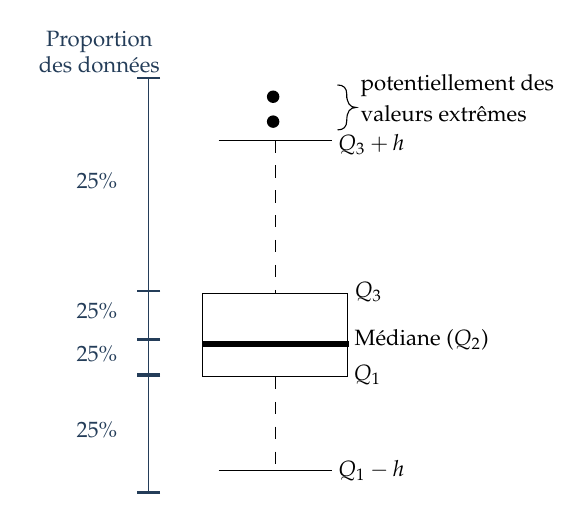
\begin{tikzpicture}[x=0.75pt,y=0.75pt,yscale=-1,xscale=1]
%uncomment if require: \path (0,300); %set diagram left start at 0, and has height of 300

%Straight Lines [id:da129737114081373] 
\draw  [dash pattern={on 4.5pt off 4.5pt}]  (181,70) -- (181,144) ;
%Straight Lines [id:da6241443915481115] 
\draw  [dash pattern={on 4.5pt off 4.5pt}]  (181,184) -- (181,229) ;
%Shape: Rectangle [id:dp9646011782302748] 
\draw   (146,144) -- (216,144) -- (216,184) -- (146,184) -- cycle ;
%Straight Lines [id:da9057676058861892] 
\draw    (153.75,229) -- (208.25,229) ;
%Straight Lines [id:da28703820276341374] 
\draw    (153.75,70) -- (208.25,70) ;
%Straight Lines [id:da23169419071689368] 
\draw [line width=2.25]    (145.75,168) -- (216.5,168) ;
%Shape: Circle [id:dp21208293035447068] 
\draw  [draw opacity=0][fill={rgb, 255:red, 0; green, 0; blue, 0 }  ,fill opacity=1 ] (177,61) .. controls (177,59.34) and (178.34,58) .. (180,58) .. controls (181.66,58) and (183,59.34) .. (183,61) .. controls (183,62.66) and (181.66,64) .. (180,64) .. controls (178.34,64) and (177,62.66) .. (177,61) -- cycle ;
%Shape: Circle [id:dp06804994911291695] 
\draw  [draw opacity=0][fill={rgb, 255:red, 0; green, 0; blue, 0 }  ,fill opacity=1 ] (177,49) .. controls (177,47.34) and (178.34,46) .. (180,46) .. controls (181.66,46) and (183,47.34) .. (183,49) .. controls (183,50.66) and (181.66,52) .. (180,52) .. controls (178.34,52) and (177,50.66) .. (177,49) -- cycle ;
%Shape: Brace [id:dp16337358256224843] 
\draw   (211,65) .. controls (213.97,65) and (215.46,63.51) .. (215.46,60.54) -- (215.46,60.54) .. controls (215.46,56.29) and (216.95,54.17) .. (219.92,54.17) .. controls (216.95,54.17) and (215.46,52.04) .. (215.46,47.79)(215.46,49.71) -- (215.46,47.79) .. controls (215.46,44.82) and (213.97,43.33) .. (211,43.33) ;
%Straight Lines [id:da0690372797278489] 
\draw [color={rgb, 255:red, 36; green, 61; blue, 89 }  ,draw opacity=1 ]   (120,40) -- (120,142.67) ;
\draw [shift={(120,142.67)}, rotate = 270] [color={rgb, 255:red, 36; green, 61; blue, 89 }  ,draw opacity=1 ][line width=0.75]    (0,5.59) -- (0,-5.59)   ;
\draw [shift={(120,40)}, rotate = 270] [color={rgb, 255:red, 36; green, 61; blue, 89 }  ,draw opacity=1 ][line width=0.75]    (0,5.59) -- (0,-5.59)   ;
%Straight Lines [id:da0032989468420259183] 
\draw [color={rgb, 255:red, 36; green, 61; blue, 89 }  ,draw opacity=1 ]   (120,142.67) -- (120,165.67) ;
\draw [shift={(120,165.67)}, rotate = 270] [color={rgb, 255:red, 36; green, 61; blue, 89 }  ,draw opacity=1 ][line width=0.75]    (0,5.59) -- (0,-5.59)   ;
\draw [shift={(120,142.67)}, rotate = 270] [color={rgb, 255:red, 36; green, 61; blue, 89 }  ,draw opacity=1 ][line width=0.75]    (0,5.59) -- (0,-5.59)   ;
%Straight Lines [id:da7171607128941915] 
\draw [color={rgb, 255:red, 36; green, 61; blue, 89 }  ,draw opacity=1 ]   (120,166.33) -- (120,183.33) ;
\draw [shift={(120,183.33)}, rotate = 270] [color={rgb, 255:red, 36; green, 61; blue, 89 }  ,draw opacity=1 ][line width=0.75]    (0,5.59) -- (0,-5.59)   ;
\draw [shift={(120,166.33)}, rotate = 270] [color={rgb, 255:red, 36; green, 61; blue, 89 }  ,draw opacity=1 ][line width=0.75]    (0,5.59) -- (0,-5.59)   ;
%Straight Lines [id:da8789207501910292] 
\draw [color={rgb, 255:red, 36; green, 61; blue, 89 }  ,draw opacity=1 ]   (120,182.67) -- (120,239.67) ;
\draw [shift={(120,239.67)}, rotate = 270] [color={rgb, 255:red, 36; green, 61; blue, 89 }  ,draw opacity=1 ][line width=0.75]    (0,5.59) -- (0,-5.59)   ;
\draw [shift={(120,182.67)}, rotate = 270] [color={rgb, 255:red, 36; green, 61; blue, 89 }  ,draw opacity=1 ][line width=0.75]    (0,5.59) -- (0,-5.59)   ;

% Text Node
\draw (221,37) node [anchor=north west][inner sep=0.75pt] [font=\footnotesize]  [align=left] {
\shortstack[l]{potentiellement des\\ valeurs extrêmes}};
% Text Node
\draw (218,137) node [anchor=north west][inner sep=0.75pt]  [font=\footnotesize] [align=left] {$\displaystyle Q_{3}$};
% Text Node
\draw (217.5,177) node [anchor=north west][inner sep=0.75pt]  [font=\footnotesize] [align=left] {$\displaystyle Q_{1}$};
% Text Node
\draw (218,160) node [anchor=north west][inner sep=0.75pt]  [font=\footnotesize] [align=left] {Médiane ($\displaystyle Q_{2}$)};
% Text Node
\draw (62,16) node [anchor=north west][inner sep=0.75pt]  [font=\footnotesize,color={rgb, 255:red, 36; green, 61; blue, 89 }  ,opacity=1 ] [align=left] {\begin{minipage}[lt]{49.455856000000004pt}\setlength\topsep{0pt}
\begin{center}
Proportion \\des données
\end{center}
\end{minipage}};
% Text Node
\draw (84,84.33) node [anchor=north west][inner sep=0.75pt]  [font=\footnotesize,color={rgb, 255:red, 36; green, 61; blue, 89 }  ,opacity=1 ] [align=left] {$\displaystyle 25\%$};
% Text Node
\draw (84,147.17) node [anchor=north west][inner sep=0.75pt]  [font=\footnotesize,color={rgb, 255:red, 36; green, 61; blue, 89 }  ,opacity=1 ] [align=left] {$\displaystyle 25\%$};
% Text Node
\draw (84,167.83) node [anchor=north west][inner sep=0.75pt]  [font=\footnotesize,color={rgb, 255:red, 36; green, 61; blue, 89 }  ,opacity=1 ] [align=left] {$\displaystyle 25\%$};
% Text Node
\draw (84,204.17) node [anchor=north west][inner sep=0.75pt]  [font=\footnotesize,color={rgb, 255:red, 36; green, 61; blue, 89 }  ,opacity=1 ] [align=left] {$\displaystyle 25\%$};
% Text Node
\draw (210,66) node [anchor=north west][inner sep=0.75pt]  [font=\footnotesize] [align=left] {$\displaystyle Q_{3} +h$};
% Text Node
\draw (210,223) node [anchor=north west][inner sep=0.75pt]  [font=\footnotesize] [align=left] {$\displaystyle Q_{1} -h$};
\end{tikzpicture}
\end{center}

\begin{itemize}
	\item	La médiane est la ligne contenue dans la boîte.
		\begin{itemize}
		\item	La moitié des données sont au-dessus, et l'autre moitié en dessous, de la ligne.
		\end{itemize}
	\item	La boîte est délimitée par le premier et le troisième quartile.
		\begin{itemize}
		\item	Il s'ensuit que la boîte contient la moitié des données.
		\item	De plus, 25\% des données sont contenues entre la borne \textit{supérieure} de la boîte et la médiane avec l'autre 25\% qui est contenu entre la borne \textit{inférieure} et la médiane.
		\end{itemize}
	\item	Les « moustaches » de la boîte sont tracées à un pas $h$ des quartiles où \lfbox[conditions]{$h = 1.5 \cdot (Q_{3} - Q_{1})$}.
		\begin{itemize}
		\item	Les points qui sont à l'extérieur de ces bornes sont les données potentiellement aberrantes.
		\item	$Q_{3}	-	Q_{1}$ correspond à l'écart interquartile.
		\item	Plus l'écart est élevé, plus la boîte sera large et, par conséquent, plus les moustaches seront situées loin de la médiane.
		\item	Le 1.5 est basé sur la règle du 68-95-99.7 avec moins de 1\% des données à l'extérieur de la borne supérieure.
		\end{itemize}
\end{itemize}

\begin{definitionNOHFILLprop}[Règle du 68-95-99.7]
Pour une distribution normale, environ 68\% des données sont en dedans d'un écart-type de la moyenne, 95\% en dedans de 2 et 99.7\% en dedans de 3.

\begin{center}
		
\tikzset{every picture/.style={line width=0.75pt}} %set default line width to 0.75pt        

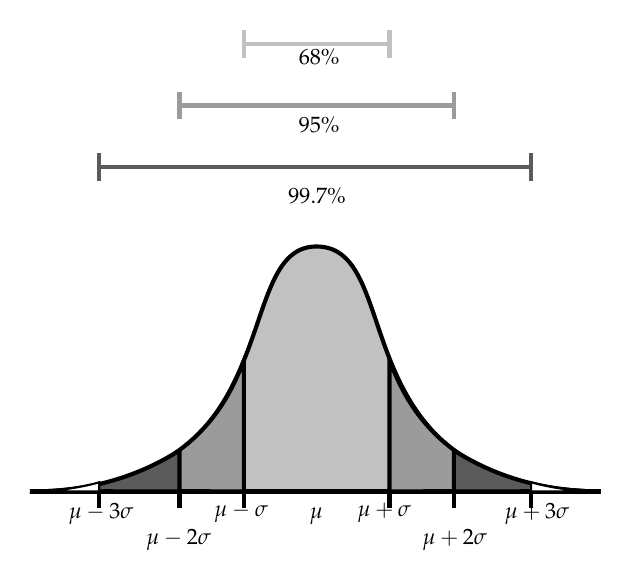
\begin{tikzpicture}[x=0.75pt,y=0.75pt,yscale=-1,xscale=1]
%uncomment if require: \path (0,278); %set diagram left start at 0, and has height of 278

%Curve Lines [id:da8749420139531441] 
\draw [draw opacity=0][fill={rgb, 255:red, 193; green, 193; blue, 193 }  ,fill opacity=1 ][line width=1.5]    (389,225.7) .. controls (520.68,226.75) and (483.98,107.66) .. (527.13,107.66) .. controls (571.77,107.66) and (537.05,225.26) .. (664.02,225.7) ;
%Straight Lines [id:da8888686520092737] 
\draw [line width=1.5]    (422.48,225.7) -- (422.48,233.64) ;
%Straight Lines [id:da1699364296805208] 
\draw [line width=1.5]    (593.34,225.7) -- (593.34,233.64) ;
%Curve Lines [id:da41861109546010566] 
\draw [line width=1.5]    (389,225.7) .. controls (517.71,227.49) and (483.98,107.66) .. (527.13,107.66) .. controls (571.77,107.66) and (536.06,225.21) .. (664.02,225.7) ;
%Straight Lines [id:da8400965165974321] 
\draw [line width=1.5]    (389,225.7) -- (664.02,225.7) ;
%Shape: Regular Polygon [id:dp11998667280876218] 
\draw  [fill={rgb, 255:red, 155; green, 155; blue, 155 }  ,fill opacity=1 ][line width=1.5]  (664.02,225.7) .. controls (584.29,225.26) and (568.2,176.16) .. (562.34,162.77) .. controls (562.34,225.26) and (562.34,162.77) .. (562.34,225.7) .. controls (663.29,225.26) and (562.34,225.26) .. (664.02,225.7) -- cycle ;
%Shape: Regular Polygon [id:dp898895201503896] 
\draw  [fill={rgb, 255:red, 155; green, 155; blue, 155 }  ,fill opacity=1 ][line width=1.5]  (390.49,225.7) .. controls (470.22,225.26) and (486.31,176.16) .. (492.16,162.77) .. controls (492.16,225.26) and (492.16,162.77) .. (492.16,225.7) .. controls (391.22,225.26) and (492.16,225.26) .. (390.49,225.7) -- cycle ;
%Shape: Regular Polygon [id:dp6032696284614307] 
\draw  [fill={rgb, 255:red, 91; green, 91; blue, 91 }  ,fill opacity=1 ][line width=1.5]  (391.98,225.7) .. controls (426.94,225.26) and (449.26,213.36) .. (461.16,205.92) .. controls (461.16,225.26) and (461.16,205.92) .. (461.16,225.7) .. controls (392.47,225.58) and (461.16,225.58) .. (391.98,225.7) -- cycle ;
%Shape: Regular Polygon [id:dp8816872519073748] 
\draw  [fill={rgb, 255:red, 91; green, 91; blue, 91 }  ,fill opacity=1 ][line width=1.5]  (662.53,225.7) .. controls (627.57,225.26) and (605.25,213.36) .. (593.34,205.92) .. controls (593.34,225.26) and (593.34,205.92) .. (593.34,225.7) .. controls (662.03,225.58) and (593.34,225.58) .. (662.53,225.7) -- cycle ;
%Shape: Polygon Curved [id:ds6677084709851981] 
\draw  [fill={rgb, 255:red, 255; green, 255; blue, 255 }  ,fill opacity=1 ][line width=0.75]  (391.98,225.7) .. controls (403.14,225.7) and (417.23,222.92) .. (422.48,221.24) .. controls (422.48,225.6) and (422.48,221.24) .. (422.48,225.7) .. controls (392.2,225.67) and (422.48,225.7) .. (391.98,225.7) -- cycle ;
%Shape: Regular Polygon [id:dp8410749943461926] 
\draw  [fill={rgb, 255:red, 255; green, 255; blue, 255 }  ,fill opacity=1 ][line width=0.75]  (661.04,225.7) .. controls (649.88,225.7) and (635.79,222.92) .. (630.54,221.24) .. controls (630.54,225.6) and (630.54,221.24) .. (630.54,225.7) .. controls (660.82,225.67) and (630.54,225.7) .. (661.04,225.7) -- cycle ;
%Straight Lines [id:da38668537998939256] 
\draw [line width=1.5]    (461.16,225.7) -- (461.16,233.64) ;
%Straight Lines [id:da1998162556500347] 
\draw [line width=1.5]    (492.16,225.7) -- (492.16,233.64) ;
%Straight Lines [id:da12951125252628293] 
\draw [line width=1.5]    (562.34,225.7) -- (562.34,233.64) ;
%Straight Lines [id:da4432220170088057] 
\draw [line width=1.5]    (630.54,225.7) -- (630.54,233.64) ;
%Straight Lines [id:da9928263828524586] 
\draw [color={rgb, 255:red, 193; green, 193; blue, 193 }  ,draw opacity=1 ][line width=1.5]    (562.34,9.95) -- (492.16,9.95) ;
\draw [shift={(492.16,9.95)}, rotate = 360] [color={rgb, 255:red, 193; green, 193; blue, 193 }  ,draw opacity=1 ][line width=1.5]    (0,6.71) -- (0,-6.71)   ;
\draw [shift={(562.34,9.95)}, rotate = 360] [color={rgb, 255:red, 193; green, 193; blue, 193 }  ,draw opacity=1 ][line width=1.5]    (0,6.71) -- (0,-6.71)   ;
%Straight Lines [id:da37156360440094294] 
\draw [color={rgb, 255:red, 155; green, 155; blue, 155 }  ,draw opacity=1 ][line width=1.5]    (593.34,39.71) -- (461.16,39.71) ;
\draw [shift={(461.16,39.71)}, rotate = 360] [color={rgb, 255:red, 155; green, 155; blue, 155 }  ,draw opacity=1 ][line width=1.5]    (0,6.71) -- (0,-6.71)   ;
\draw [shift={(593.34,39.71)}, rotate = 360] [color={rgb, 255:red, 155; green, 155; blue, 155 }  ,draw opacity=1 ][line width=1.5]    (0,6.71) -- (0,-6.71)   ;
%Straight Lines [id:da8337470834507461] 
\draw [color={rgb, 255:red, 91; green, 91; blue, 91 }  ,draw opacity=1 ][line width=1.5]    (630.54,69.47) -- (422.48,69.47) ;
\draw [shift={(422.48,69.47)}, rotate = 360] [color={rgb, 255:red, 91; green, 91; blue, 91 }  ,draw opacity=1 ][line width=1.5]    (0,6.71) -- (0,-6.71)   ;
\draw [shift={(630.54,69.47)}, rotate = 360] [color={rgb, 255:red, 91; green, 91; blue, 91 }  ,draw opacity=1 ][line width=1.5]    (0,6.71) -- (0,-6.71)   ;

% Text Node
\draw (522.62,232.23) node [anchor=north west][inner sep=0.75pt]   [align=left] {{\footnotesize $\displaystyle \mu $}};
% Text Node
\draw (545.6,230.23) node [anchor=north west][inner sep=0.75pt]   [align=left] {{\footnotesize $\displaystyle \mu +\sigma $}};
% Text Node
\draw (576.84,242.62) node [anchor=north west][inner sep=0.75pt]  [font=\normalsize] [align=left] {{\footnotesize $\displaystyle \mu +2\sigma $}};
% Text Node
\draw (616.5,230.23) node [anchor=north west][inner sep=0.75pt]   [align=left] {{\footnotesize $\displaystyle \mu +3\sigma $}};
% Text Node
\draw (517.35,11.12) node [anchor=north west][inner sep=0.75pt]   [align=left] {{\footnotesize 68\%}};
% Text Node
\draw (517.35,43.86) node [anchor=north west][inner sep=0.75pt]   [align=left] {{\footnotesize 95\%}};
% Text Node
\draw (512.35,78.08) node [anchor=north west][inner sep=0.75pt]   [align=left] {{\footnotesize 99.7\%}};
% Text Node
\draw (476.6,230.23) node [anchor=north west][inner sep=0.75pt]   [align=left] {{\footnotesize $\displaystyle \mu -\sigma $}};
% Text Node
\draw (443.84,242.62) node [anchor=north west][inner sep=0.75pt]  [font=\normalsize] [align=left] {{\footnotesize $\displaystyle \mu -2\sigma $}};
% Text Node
\draw (406.5,230.23) node [anchor=north west][inner sep=0.75pt]   [align=left] {{\footnotesize $\displaystyle \mu -3\sigma $}};
\end{tikzpicture}

\end{center}
\end{definitionNOHFILLprop}

\columnbreak
En bref, le diagramme en boîte permet d'évaluer comment les données sont distribuées. Cette image de \href{https://en.wikipedia.org/wiki/Interquartile_range}{wikipedia} résume bien : 
\begin{center}
	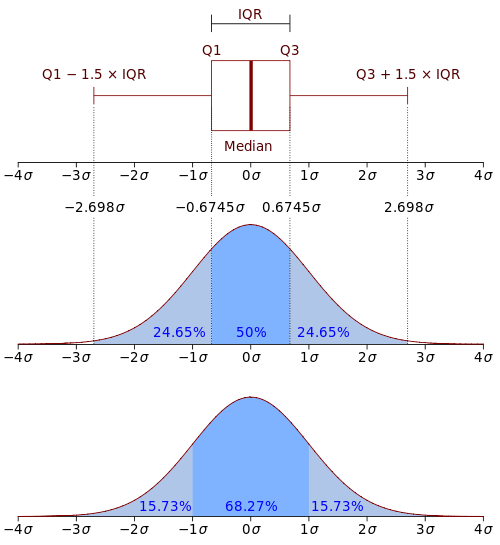
\includegraphics[scale=0.4]{../../src/ACT-2000/boxplot-normrule.png}
\end{center}


\columnbreak
\subsubsection{Diagramme quantile-quantile (\og \textit{Q-Q plot} \fg{})}
En pratique, on pose souvent que les données suivent une distribution. Un diagramme quantile-quantile permet de comparer les quantiles théoriques de la distribution aux quantiles empiriques des données. \\

Dans un tel cas, on connaît la distribution, mais pas les paramètres.
\begin{itemize}
	\item	Si les données sont normalement distribuées, on peut centrer et réduire pour obtenir la loi normale standard $Z$ ; 
		\begin{itemize}
		\item	Ceci correspond à un diagramme quantile-quantile \textbf{normale} ;
		\end{itemize}
	\item	Autrement, le diagramme quantile-quantile est tracé en estimant les paramètres de la distribution avec l'échantillon de données.
\end{itemize}

\

Par exemple :
\begin{center}
\tikzset{every picture/.style={line width=0.75pt}} %set default line width to 0.75pt        

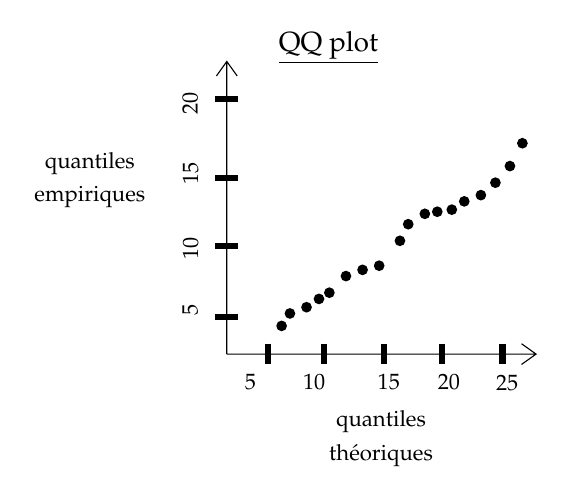
\begin{tikzpicture}[x=0.75pt,y=0.75pt,yscale=-1,xscale=1]
%uncomment if require: \path (0,300); %set diagram left start at 0, and has height of 300

%Shape: Axis 2D [id:dp6907328462183413] 
\draw  (159.17,162) -- (308.17,162)(159.17,21) -- (159.17,162) -- cycle (301.17,157) -- (308.17,162) -- (301.17,167) (154.17,28) -- (159.17,21) -- (164.17,28)  ;
%Straight Lines [id:da2684391209424455] 
\draw [line width=2.25]    (179,157) -- (179,167) ;
%Straight Lines [id:da26665731526815106] 
\draw [line width=2.25]    (206,157) -- (206,167) ;
%Straight Lines [id:da5458795480754546] 
\draw [line width=2.25]    (235,157) -- (235,167) ;
%Straight Lines [id:da7749608799910399] 
\draw [line width=2.25]    (263,157) -- (263,167) ;
%Straight Lines [id:da781366529806411] 
\draw [line width=2.25]    (292,157) -- (292,167) ;
%Straight Lines [id:da5656665110363344] 
\draw [line width=2.25]    (153.67,39) -- (164.5,39) ;
%Straight Lines [id:da06457141428798874] 
\draw [line width=2.25]    (153.67,77) -- (164.5,77) ;
%Straight Lines [id:da07440013590512717] 
\draw [line width=2.25]    (153.67,110) -- (164.5,110) ;
%Straight Lines [id:da7046117446976516] 
\draw [line width=2.25]    (153.67,144) -- (164.5,144) ;
%Flowchart: Connector [id:dp26709638677620307] 
\draw  [draw opacity=0][fill={rgb, 255:red, 0; green, 0; blue, 0 }  ,fill opacity=1 ] (187,142.42) .. controls (187,140.99) and (188.16,139.83) .. (189.58,139.83) .. controls (191.01,139.83) and (192.17,140.99) .. (192.17,142.42) .. controls (192.17,143.84) and (191.01,145) .. (189.58,145) .. controls (188.16,145) and (187,143.84) .. (187,142.42) -- cycle ;
%Flowchart: Connector [id:dp9807914547061263] 
\draw  [draw opacity=0][fill={rgb, 255:red, 0; green, 0; blue, 0 }  ,fill opacity=1 ] (183,148.42) .. controls (183,146.99) and (184.16,145.83) .. (185.58,145.83) .. controls (187.01,145.83) and (188.17,146.99) .. (188.17,148.42) .. controls (188.17,149.84) and (187.01,151) .. (185.58,151) .. controls (184.16,151) and (183,149.84) .. (183,148.42) -- cycle ;
%Flowchart: Connector [id:dp15148611073322638] 
\draw  [draw opacity=0][fill={rgb, 255:red, 0; green, 0; blue, 0 }  ,fill opacity=1 ] (195,139.42) .. controls (195,137.99) and (196.16,136.83) .. (197.58,136.83) .. controls (199.01,136.83) and (200.17,137.99) .. (200.17,139.42) .. controls (200.17,140.84) and (199.01,142) .. (197.58,142) .. controls (196.16,142) and (195,140.84) .. (195,139.42) -- cycle ;
%Flowchart: Connector [id:dp8718571676300524] 
\draw  [draw opacity=0][fill={rgb, 255:red, 0; green, 0; blue, 0 }  ,fill opacity=1 ] (201,135.42) .. controls (201,133.99) and (202.16,132.83) .. (203.58,132.83) .. controls (205.01,132.83) and (206.17,133.99) .. (206.17,135.42) .. controls (206.17,136.84) and (205.01,138) .. (203.58,138) .. controls (202.16,138) and (201,136.84) .. (201,135.42) -- cycle ;
%Flowchart: Connector [id:dp6298382695689162] 
\draw  [draw opacity=0][fill={rgb, 255:red, 0; green, 0; blue, 0 }  ,fill opacity=1 ] (206,132.42) .. controls (206,130.99) and (207.16,129.83) .. (208.58,129.83) .. controls (210.01,129.83) and (211.17,130.99) .. (211.17,132.42) .. controls (211.17,133.84) and (210.01,135) .. (208.58,135) .. controls (207.16,135) and (206,133.84) .. (206,132.42) -- cycle ;
%Flowchart: Connector [id:dp7974400157875505] 
\draw  [draw opacity=0][fill={rgb, 255:red, 0; green, 0; blue, 0 }  ,fill opacity=1 ] (214,124.42) .. controls (214,122.99) and (215.16,121.83) .. (216.58,121.83) .. controls (218.01,121.83) and (219.17,122.99) .. (219.17,124.42) .. controls (219.17,125.84) and (218.01,127) .. (216.58,127) .. controls (215.16,127) and (214,125.84) .. (214,124.42) -- cycle ;
%Flowchart: Connector [id:dp18385794853649817] 
\draw  [draw opacity=0][fill={rgb, 255:red, 0; green, 0; blue, 0 }  ,fill opacity=1 ] (222,121.42) .. controls (222,119.99) and (223.16,118.83) .. (224.58,118.83) .. controls (226.01,118.83) and (227.17,119.99) .. (227.17,121.42) .. controls (227.17,122.84) and (226.01,124) .. (224.58,124) .. controls (223.16,124) and (222,122.84) .. (222,121.42) -- cycle ;
%Flowchart: Connector [id:dp41038901090251567] 
\draw  [draw opacity=0][fill={rgb, 255:red, 0; green, 0; blue, 0 }  ,fill opacity=1 ] (230,119.42) .. controls (230,117.99) and (231.16,116.83) .. (232.58,116.83) .. controls (234.01,116.83) and (235.17,117.99) .. (235.17,119.42) .. controls (235.17,120.84) and (234.01,122) .. (232.58,122) .. controls (231.16,122) and (230,120.84) .. (230,119.42) -- cycle ;
%Flowchart: Connector [id:dp9668794505330132] 
\draw  [draw opacity=0][fill={rgb, 255:red, 0; green, 0; blue, 0 }  ,fill opacity=1 ] (240,107.42) .. controls (240,105.99) and (241.16,104.83) .. (242.58,104.83) .. controls (244.01,104.83) and (245.17,105.99) .. (245.17,107.42) .. controls (245.17,108.84) and (244.01,110) .. (242.58,110) .. controls (241.16,110) and (240,108.84) .. (240,107.42) -- cycle ;
%Flowchart: Connector [id:dp23760159423012994] 
\draw  [draw opacity=0][fill={rgb, 255:red, 0; green, 0; blue, 0 }  ,fill opacity=1 ] (244,99.42) .. controls (244,97.99) and (245.16,96.83) .. (246.58,96.83) .. controls (248.01,96.83) and (249.17,97.99) .. (249.17,99.42) .. controls (249.17,100.84) and (248.01,102) .. (246.58,102) .. controls (245.16,102) and (244,100.84) .. (244,99.42) -- cycle ;
%Flowchart: Connector [id:dp9760550495862494] 
\draw  [draw opacity=0][fill={rgb, 255:red, 0; green, 0; blue, 0 }  ,fill opacity=1 ] (252,94.42) .. controls (252,92.99) and (253.16,91.83) .. (254.58,91.83) .. controls (256.01,91.83) and (257.17,92.99) .. (257.17,94.42) .. controls (257.17,95.84) and (256.01,97) .. (254.58,97) .. controls (253.16,97) and (252,95.84) .. (252,94.42) -- cycle ;
%Flowchart: Connector [id:dp09806905504709196] 
\draw  [draw opacity=0][fill={rgb, 255:red, 0; green, 0; blue, 0 }  ,fill opacity=1 ] (258,93.42) .. controls (258,91.99) and (259.16,90.83) .. (260.58,90.83) .. controls (262.01,90.83) and (263.17,91.99) .. (263.17,93.42) .. controls (263.17,94.84) and (262.01,96) .. (260.58,96) .. controls (259.16,96) and (258,94.84) .. (258,93.42) -- cycle ;
%Flowchart: Connector [id:dp21547983210697952] 
\draw  [draw opacity=0][fill={rgb, 255:red, 0; green, 0; blue, 0 }  ,fill opacity=1 ] (265,92.42) .. controls (265,90.99) and (266.16,89.83) .. (267.58,89.83) .. controls (269.01,89.83) and (270.17,90.99) .. (270.17,92.42) .. controls (270.17,93.84) and (269.01,95) .. (267.58,95) .. controls (266.16,95) and (265,93.84) .. (265,92.42) -- cycle ;
%Flowchart: Connector [id:dp13436174967362358] 
\draw  [draw opacity=0][fill={rgb, 255:red, 0; green, 0; blue, 0 }  ,fill opacity=1 ] (271,88.42) .. controls (271,86.99) and (272.16,85.83) .. (273.58,85.83) .. controls (275.01,85.83) and (276.17,86.99) .. (276.17,88.42) .. controls (276.17,89.84) and (275.01,91) .. (273.58,91) .. controls (272.16,91) and (271,89.84) .. (271,88.42) -- cycle ;
%Flowchart: Connector [id:dp6321990138892946] 
\draw  [draw opacity=0][fill={rgb, 255:red, 0; green, 0; blue, 0 }  ,fill opacity=1 ] (279,85.42) .. controls (279,83.99) and (280.16,82.83) .. (281.58,82.83) .. controls (283.01,82.83) and (284.17,83.99) .. (284.17,85.42) .. controls (284.17,86.84) and (283.01,88) .. (281.58,88) .. controls (280.16,88) and (279,86.84) .. (279,85.42) -- cycle ;
%Flowchart: Connector [id:dp8650742018499089] 
\draw  [draw opacity=0][fill={rgb, 255:red, 0; green, 0; blue, 0 }  ,fill opacity=1 ] (286,79.42) .. controls (286,77.99) and (287.16,76.83) .. (288.58,76.83) .. controls (290.01,76.83) and (291.17,77.99) .. (291.17,79.42) .. controls (291.17,80.84) and (290.01,82) .. (288.58,82) .. controls (287.16,82) and (286,80.84) .. (286,79.42) -- cycle ;
%Flowchart: Connector [id:dp8249100072120605] 
\draw  [draw opacity=0][fill={rgb, 255:red, 0; green, 0; blue, 0 }  ,fill opacity=1 ] (293,71.42) .. controls (293,69.99) and (294.16,68.83) .. (295.58,68.83) .. controls (297.01,68.83) and (298.17,69.99) .. (298.17,71.42) .. controls (298.17,72.84) and (297.01,74) .. (295.58,74) .. controls (294.16,74) and (293,72.84) .. (293,71.42) -- cycle ;
%Flowchart: Connector [id:dp5353454981608219] 
\draw  [draw opacity=0][fill={rgb, 255:red, 0; green, 0; blue, 0 }  ,fill opacity=1 ] (299,60.42) .. controls (299,58.99) and (300.16,57.83) .. (301.58,57.83) .. controls (303.01,57.83) and (304.17,58.99) .. (304.17,60.42) .. controls (304.17,61.84) and (303.01,63) .. (301.58,63) .. controls (300.16,63) and (299,61.84) .. (299,60.42) -- cycle ;


% Text Node
\draw (183,5) node [anchor=north west][inner sep=0.75pt]   [align=left] {\underline{QQ plot}};
% Text Node
\draw (205,188) node [anchor=north west][inner sep=0.75pt]   [align=left] {\begin{minipage}[lt]{40.828356pt}\setlength\topsep{0pt}
\begin{center}
{\footnotesize quantiles }\\{\footnotesize théoriques}
\end{center}

\end{minipage}};
% Text Node
\draw (63.5,63.5) node [anchor=north west][inner sep=0.75pt]   [align=left] {\begin{minipage}[lt]{42.634572pt}\setlength\topsep{0pt}
\begin{center}
{\footnotesize quantiles }\\{\footnotesize empiriques}
\end{center}

\end{minipage}};
% Text Node
\draw (166.62,170.3) node [anchor=north west][inner sep=0.75pt]  [font=\footnotesize] [align=left] {$\displaystyle 5$};
% Text Node
\draw (194.62,170.3) node [anchor=north west][inner sep=0.75pt]  [font=\footnotesize] [align=left] {$\displaystyle 10$};
% Text Node
\draw (230.62,170.3) node [anchor=north west][inner sep=0.75pt]  [font=\footnotesize] [align=left] {$\displaystyle 15$};
% Text Node
\draw (259.62,170.3) node [anchor=north west][inner sep=0.75pt]  [font=\footnotesize] [align=left] {$\displaystyle 20$};
% Text Node
\draw (287.62,170.8) node [anchor=north west][inner sep=0.75pt]  [font=\footnotesize] [align=left] {$\displaystyle 25$};
% Text Node
\draw (136.62,144.8) node [anchor=north west][inner sep=0.75pt]  [font=\footnotesize,rotate=-270] [align=left] {$\displaystyle 5$};
% Text Node
\draw (136.62,117.8) node [anchor=north west][inner sep=0.75pt]  [font=\footnotesize,rotate=-270] [align=left] {$\displaystyle 10$};
% Text Node
\draw (136.62,81.8) node [anchor=north west][inner sep=0.75pt]  [font=\footnotesize,rotate=-270] [align=left] {$\displaystyle 15$};
% Text Node
\draw (136.62,47.8) node [anchor=north west][inner sep=0.75pt]  [font=\footnotesize,rotate=-270] [align=left] {$\displaystyle 20$};
\end{tikzpicture}

\end{center}

Le diagramme quantile-quantile évalue si la distribution empirique est semblable à la distribution théorique. On peut, entre autres, évaluer la queue de la distribution. Selon la distribution, les quantiles « normaux » varient. Ci-dessous est une image de \href{https://mgimond.github.io/ES218/Week06a.html}{ce site} qui montre quantiles selon la distribution avec une droite pour la normale :
\begin{center}
	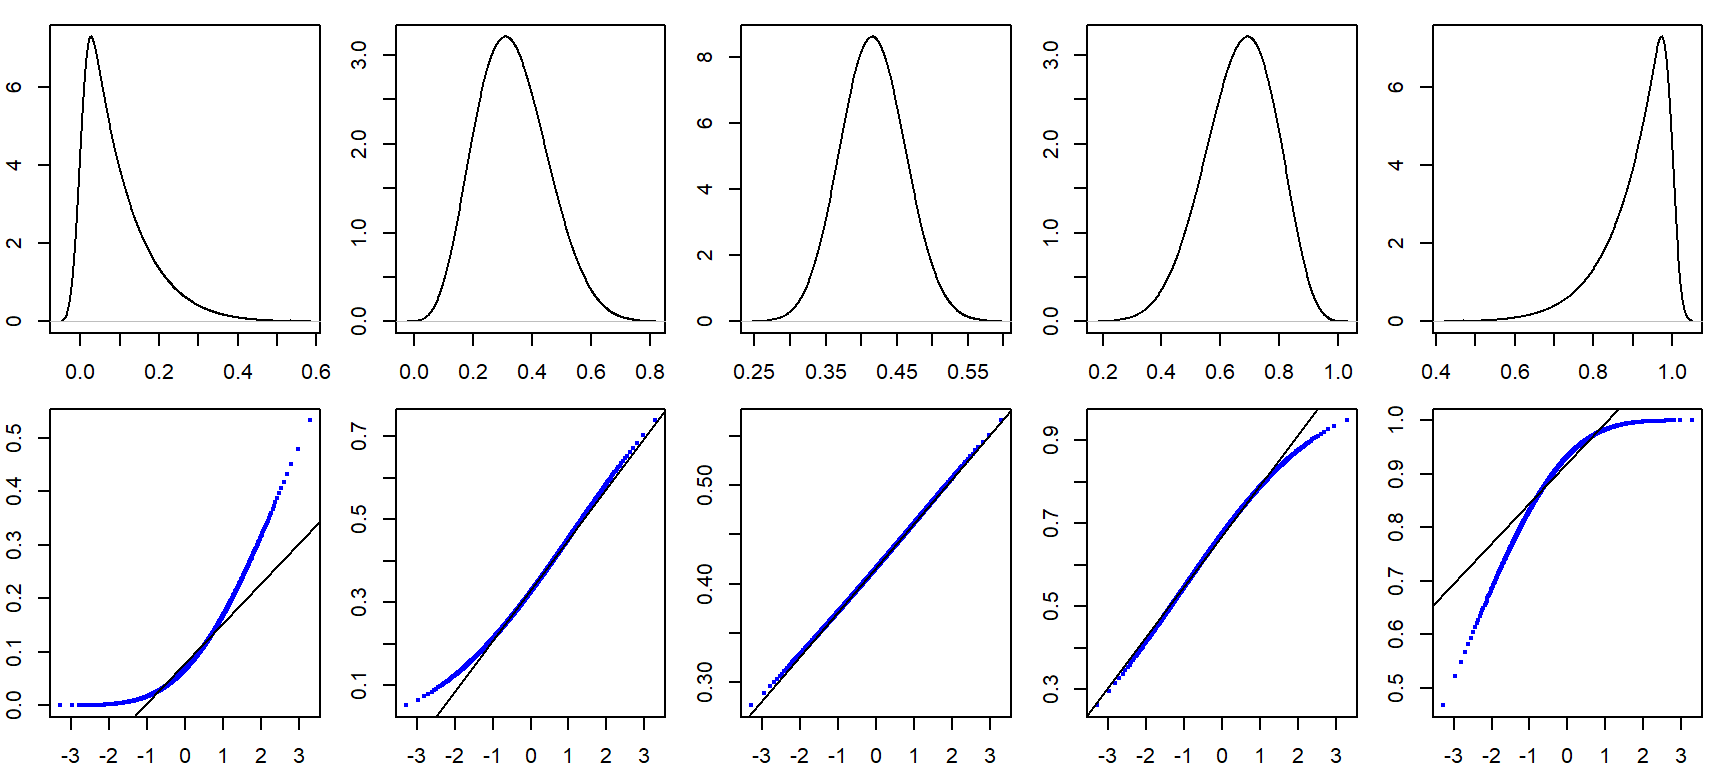
\includegraphics[scale=0.5]{../../src/ACT-2000/qqplot-skeweing.png}
\end{center}


\columnbreak
\section{Construction d'estimateurs}
\subsection{Introduction}
\begin{rappel_enhanced}[Contexte]
Plus tôt, nous avons décrit les méthodes utilisées pour évaluer la \textbf{qualité} d'un estimateur. Cependant, nous n'avons pas décrit comment obtenir ces estimateurs. Non seulement il y a une panoplie de façons de construire un estimateur, mais aussi de façons d'estimer des paramètres. \\

La méthode vue dans le cadre du cours de statistique (et de l'examen MAS-I) est la méthode dite « \textbf{fréquentiste} ». Le cours de \nameref{chapt:mathIARD} présente \textbf{l'estimation bayésienne}.
\end{rappel_enhanced}


Dans le contexte de l'examen, nous voyons 3 méthodes. Les deux premières (méthode des moments et du « percentile matching ») sont les plus faciles à obtenir. Cependant, elles sont aussi les méthodes d'estimation les moins précises car elles utilisent seulement une \textit{portion} des données. En revanche, la méthode du maximum de vraisemblance utilise \textit{toutes} les données.	\\

Cette distinction devient particulièrement importante dans le cas d'une distribution avec une queue de droite lourde (e.g. Pareto, Weibull, etc.). Pour ces distributions, il est essentiel de connaître  précisément les valeurs extrêmes afin de bien estimer le(s) paramètre(s) de forme.	\\

Les deux premières méthodes comporte également la limitation que les données doivent toutes provenir de la même distribution. Autrement, il ne serait pas clair ce que sont les moments et quantiles. Finalement, les deux premières méthodes peuvent être manipulées car car la décision de quels moments et centiles à utiliser est \textit{arbitraire}.



\columnbreak
\subsection{Méthode des moments (MoM)}
\begin{distributions}[Terminologie]
\begin{description}
	\item[$\mu_{k}'(\hat{\theta})$]	$k^{\text{e}}$ moment centré à 0, \icbox{$\mu_{k}' = \text{E}[X^{k}]$}.
	\item[]	$\equalhat$	Notation pour poser une égalité.
\end{description}
\end{distributions}


\begin{definitionNOHFILL}[Méthode des moments (MoM)]
\begin{rappel_enhanced}[Contexte]
La méthode des moments applique l'idée, ou « hypothèse », qu'un échantillon de données devrait être semblable à sa distribution posée. Elle estime les paramètres avec les moments empiriques sous l'hypothèse que les moments empiriques devraient, en théorie, être égaux aux moments théoriques.
\end{rappel_enhanced}

On \textcolor{teal}{pose} les $r$ premiers \textcolor{amethyst}{moments empiriques} de l'échantillon égaux aux $r$ premiers \textcolor{trueblue}{moments théoriques} d'une distribution $X$ ayant $r$ paramètres $\bm{\theta}$. \\

L'estimation de $\bm{\theta}$ est donc la solution aux $r$ équations suivantes : 
\begin{equation*}
	\textcolor{amethyst}{\hat{\mu}_{k}'} 
	=	\frac{1}{n}\sum_{i = 1}^{n} x_{i}^{k}\
	\textcolor{teal}{\equalhat}\	\esp{X^{k}}
	=	\textcolor{trueblue}{\mu_{k}'(\theta)}, \quad	k = 1, 2, \dots, r
\end{equation*}
\end{definitionNOHFILL}



\columnbreak
\subsection{Méthode du \guillemotleft Percentile Matching \guillemotright}
\begin{distributions}[Notation]
\begin{description}
	\item[$\pi_{q}(\bm{\theta})$]	$100q^{\text{e}}$ centile, \lfbox[formula]{$\pi_{q}(\bm{\theta}) = F^{-1}_{\bm{\theta}}(q)$}, \lfbox[conditions]{$q \in [0, 1]$}.
\end{description}
\end{distributions}

\begin{definitionNOHFILL}[Méthode du \og \textit{percentile matching} \fg{}]
\begin{rappel_enhanced}[Contexte]
La méthode du \og \textit{percentile matching} \fg{} estime les paramètres avec les centiles empiriques sous l'hypothèse que les centiles empiriques devraient, en théorie, être égaux aux centiles théoriques.\\

Un désavantage de cette méthode est le choix des centiles à utiliser arbitraire. Ceci peut mener à des manipulations des données. Dans le contexte d'un examen cependant, les centiles à utiliser seront spécifiés.
\end{rappel_enhanced}

On \textcolor{teal}{pose} $r$ \textcolor{amethyst}{centiles empiriques} de l'échantillon égaux aux $r$ \textcolor{trueblue}{centiles théoriques} correspondants d'une distribution $X$ ayant $r$ paramètres $\bm{\theta}$. \\

L'estimation de $\bm{\theta}$ est donc la solution aux $r$ équations suivantes : 
\begin{equation*}
	\textcolor{amethyst}{\hat{\pi}_{q_{k}} | \theta)}\
	\textcolor{teal}{\equalhat}\	
	\textcolor{trueblue}{\pi_{q_{k}}}, \quad	k = 1, 2, \dots, r
\end{equation*}
\end{definitionNOHFILL}


Cependant, nous devons calculer ces centiles ! Il y existe une myriade de façons de le faire, mais pour l'examen on utilise le  \og \textit{smoothed empirical estimate} \fg{} d'un centile. Entre autres, cette méthode permet d'interpoler des quantiles s'il n'existe pas.

%Il peut arriver que les centiles de distributions ne soient pas uniques, par exemple dans le cas de données discrètes lorsque le quantile recherché peut tomber entre 2 \emph{marches} de la fonction empirique, ou mal-définis.

\begin{definitionNOHFILLsub}[\og \textit{smoothed empirical estimate} \fg{}]
\begin{distributions}[Notation]
\begin{description}
	\item[$x_{(i)}$]	La $i^{e}$ statistique d'ordre de l'échantillon.
	\item[$b = \lfloor q (n + 1) \rfloor$]	Arrondi vers le bas du centile.
\end{description}
\end{distributions}

Étapes pour trouver les centiles : 
\begin{enumerate}[label = \circled{\arabic*}{trueblue}]
	\item	Calculer $q(n + 1)$.
	\item	Si 
		\begin{enumerate}[label = \alph*)]
		\item	$q(n + 1)$ est fractionnaire, calculer $\hat{\pi}_{q}$ comme l'interpolation linéaire de $x_{(b)}$ et $x_{(b + 1)}$.
		\item	$q(n + 1)$ est entier, poser $\hat{\pi}_{q} = x_{(b)}$.
		\end{enumerate}
\end{enumerate}

En bref, pour $h = q(n + 1) - b$, \lfbox[formula]{$\hat{\pi}_{q} = (1 - h)x_{(b)} + hx_{(b + 1)}$}.
\end{definitionNOHFILLsub}

\paragraph{Note}	Pour des valeurs répétées (deux observations de l'échantillon ont la même valeur), on ignore les observations ayant le plus gros indice. Si $x_{(2)} = x_{(3)}$ alors on ignore $x_{(3)}$ pour les interpolations.



\columnbreak
\subsection{Méthode du maximum de vraisemblance}
Nous cherchons à maximiser la probabilité d'observer les données.
Ceci est fait par la vraisemblance $\mathcal{L}(\theta; \bm{x})$ ou, puisque le logarithme ne change pas le maximum, la log-vraisemblance $\ell(\theta; x)$ où:

\begin{algo}{Maximum de vraisemblance}
\begin{align*}
	\mathcal{L}(\theta; \bm{x})
	&=	\prod_{i = 1}^{n}	f(x_{i}; \theta)	&
	&\text{et}	&
	\ell(\theta; \bm{x})
	&=	\sum_{i = 1}^{n} \ln	f(x_{i}; \theta)	&
\end{align*}
et l'\textbf{estimateur du maximum de vraisemblance} de $\bm\theta$ est celui qui maximise la fonction de vraisemblance.
\end{algo}

De façon formelle, on dit que \lfbox[formula]{$\hat{\theta}^{\text{EMV}}	=	\underset{\theta}{\max}\{\mathcal{L}(\theta; \bm{x})\}	=	\underset{\theta}{\max}\{\ln\mathcal{L}(\theta; \bm{x})\}$.}

\subsubsection{Raccourcis}

Si la fonction de vraisemblance est de la forme :
\begin{itemize}
	\item	\lfbox[formula]{$\mathcal{L}(\gamma)	=	\gamma^{-a}\textrm{e}^{-b/\gamma}$} alors \lfbox[formula]{$\hat{\gamma}^{\text{MLE}}	=	\frac{b}{a}$}.
	\item	\lfbox[formula]{$\mathcal{L}(\lambda)	=	\lambda^{a}\textrm{e}^{-\lambda b}$} alors \lfbox[formula]{$\hat{\lambda}^{\text{MLE}}	=	\frac{a}{b}$}.
	\item	\lfbox[formula]{$\mathcal{L}(\theta)	=	\theta^{a}(1	-	\theta)^{b}$} then \lfbox[formula]{$\hat{\theta}^{\text{MLE}}	=	\frac{a}{a + b}$}.
\end{itemize}


\subsubsection{Propriétés}
\begin{definitionNOHFILL}[Propriété d'invariance]
Soit une fonction bijective $g(\cdot)$ et l'estimateur du maximum de vraisemblance (EMV) $\hat{\theta}^{\text{EMV}}$ de $\theta$.\\
Alors, selon la propriété d'invariance \lfbox[formula]{$g(\hat{\theta}^{\text{EMV}})$ est l'EMV de $g(\theta)$.}\\

L'EMV satisfait cette propriété.
\end{definitionNOHFILL}

\begin{definitionNOHFILL}[Convergence en distribution de l'EMV]
\textbf{Théorème}:	\lfbox[formula]{$\hat{\theta}^{\text{EMV}}	\approx	\mathcal{N}\left(0, \frac{1}{\bm{I}_{n}(\theta)}\right)$.}

\tcbline

Sous \hyperlink{reg_cond}{\color{blue!40!green!80!black}certaines conditions de régularité}, la distribution de $\sqrt{n}\left( \hat{\theta}	-	\theta \right)$ converge en distribution vers une distribution normale avec une moyenne nulle et une variance égale à la \hyperref[sec:cramer_rao]{\color{azure(colorwheel)}borne de Cramér-Rao}.
\begin{align*}
	\sqrt{n}\left( \hat{\theta}	-	\theta \right)
	&\overset{D}{\rightarrow}
	\mathcal{N}\left( 0, \frac{1}{\bm{I}_{n}(\theta)} \right)
\end{align*}

Ce qui implique:
\begin{enumerate}
	\item	$\hat{\theta}$ est \lfbox[imphl]{asymptotiquement sans biais.}
	\item	$\hat{\theta}$ est \lfbox[imphl]{\og \textit{consistent} \fg{}.}
	\item	$\hat{\theta}$ est \lfbox[imphl]{approximativement normalement distribué avec moyenne $\theta$ et} \lfbox[imphl]{variance $1/\bm{I}_{n}(\theta)$ pour des grands échantillons.}
	\item	$\hat{\theta}$ est \lfbox[imphl]{asymptotiquement efficace} puisque sa variance tend vers la borne Cramér-Rao.
\end{enumerate}
\end{definitionNOHFILL}
	
Souvent les professeurs ne montrent pas ces conditions puisqu'elles sont compliquées. Alors, ne vous en faites pas si vous ne les comprenez pas complètement.

\begin{definitionNOHFILLsub}[\hypertarget{reg_cond}{Conditions de régularité}]
\begin{description}
	\item[R0]	Les variables $X_{i}$ sont iid avec densité $f(x_{i}; \theta)$ pour $i	=	1, 2, \dots$.
	\item[R1]	Les fonctions de densité ont toutes le même support pour tout $\theta$.
		\begin{itemize}
		\item	C'est-à-dire que le support de $X_{i}$ ne dépend pas de $\theta$;
		\item	C'est une condition restrictive que certains modèles ne respectent pas.
		\end{itemize}
	\item[R2]	La "vraie valeur" de $\theta$ est contenue dans l'ensemble des valeurs possibles $\Theta$.
\tcbline
\begin{description}
	\item[R3]	La fonction de densité $f(x; \theta)$ est différentiable deux fois comme fonction de $\theta$.
		\begin{itemize}
		\item	Cette condition additionnelle assure que les deux premières dérivées existent pour \hyperref[sec:cramer_rao]{\color{azure(colorwheel)}la borne de Cramér-Rao}.
		\end{itemize}
	\item[R4]	L'intégrale $\int f(x; \theta) dx$ est différentiable deux fois sous l'intégrale comme fonction de $\theta$.
		\begin{itemize}
		\item	Cette condition additionnelle assure que l'on peut utiliser la deuxième dérivée pour \hyperref[sec:cramer_rao]{\color{azure(colorwheel)}la borne de Cramér-Rao}.
		\end{itemize}
\end{description}
\end{description}
%%%	--------------------------------
%%%	NOTES:
%%%	+	FAUT AJOUTER DES DÉTAILS SUR LES CONDITIONS AVEC LES DÉRIVÉES D'INTÉGRALES ÉGAUX À ZÉRO!!!!!
%%%	+	Ajouter des détails sur l'efficacité asymptotique;
%%%	+	Intervalles de confiance
%%%	--------------------------------
%\begin{description}
%	\item[R5]	La fonction de densité $f(x; \theta)$ est différentiable trois fois comme fonction de $\theta$. De plus, $\forall \theta \in \Theta$ il existe une constante $c$ and une fonction $g(x)$ tel que $\big| \deriv[3]{\theta}{} \ln f(x; \theta) \big| \leq g(x)$.
%\end{description}
%%%	Impliquent que l'on peut interchanger l'intégration et la différention wrt/ \theta
\end{definitionNOHFILLsub}
	

\subsubsection{Cas multivarié}
On généralise du cas où $\theta$ est un scalaire (un seul paramètre) au cas multivarié avec $k$ paramètres et le vecteur $\bm{\theta}	=	(\theta_{1}, \cdots, \theta_{k})^{\top}$.\\


\begin{distributions}[Notation]
En notation matricielle, on multiple le vecteur $\bm{\theta}$ par la transposée $\bm{\theta}^{\top}$ au lieu de mettre $\theta$ au carré. 
\begin{itemize}
	\item	La matrice d'information Fisher \underline{d'\textit{une} observation} est donc une matrice $k \times k$:
\begin{align*}
	\bm{I}(\bm{\theta})
	&=	\text{E}\left[	
			\frac{\partial \ln f(X; \bm{\theta})}{\partial \bm{\theta}}
			\frac{\partial \ln f(X; \bm{\theta})}{\partial \bm{\theta}^{\top}}
		\right]
	\overset{iid}{=}	\text{E}\left[	
			\frac{\partial^{2} \ln f(X; \bm{\theta})}{\partial \bm{\theta}\bm{\theta}^{\top}}
		\right]
\end{align*}
%%%	------------------------
%%%	NOTES
%%%	+	Vérifier les X pour voir où les majuscules vont avec matrice d'information Fisher!!! vs f(x; \theta), f(X; \theta) ,,......\bm{X}?
%%%	------------------------
	\item	Pour la matrice d'information Fisher d'un échantillon aléatoire de $n$ observation, on utilise la relation $\bm{I}_{n}(\bm{\theta})	=	n\bm{I}(\bm{\theta})$.
\end{itemize}
\begin{description}
	\item[$\bm{I}^{-1}_{n}(\bm{\theta})$]	Inverse de la matrice d'information Fisher $\bm{I}_{n}(\bm{\theta})$.
\end{description}
\end{distributions}

Soit $\tilde{\bm{\theta}}$ un estimateur sans bais de $\bm{\theta}$. 

\begin{distributions}[Notation]
\begin{description}
	\item[$\text{Var}(\tilde{\bm{\theta}})$]	Matrice de variance de $\tilde{\bm{\theta}}$.
		\begin{itemize}
		\item	Le $(i, j)^{\text{e}}$ élément est donc $\text{Cov}(\tilde{\bm{\theta}}_{i}, \tilde{\bm{\theta}}_{j})$.
		\end{itemize}
\end{description}
\end{distributions}

La version multivariée de l'inégalité Cramér-Rao stipule que \lfbox[formula]{$\text{Var}(\tilde{\bm{\theta}})	-	\bm{I}^{-1}_{n}(\bm{\theta})$} est une \lfbox[conditions]{matrice \og \textit{nonnegative definite} \fg{}.}
\begin{itemize}
	\item	Puisque les éléments de la diagonale doivent être positifs, la borne inférieure de $\text{Var}(\tilde{\bm{\theta}}_{i})$ est le $i^{\text{e}}$ élément de la diagonale de $\bm{I}^{-1}_{n}(\bm{\theta})$.
\end{itemize}
	
En bref, on trouve que sous \hyperlink{reg_cond}{\color{blue!40!green!80!black}certaines conditions de régularité}, la distribution de $\sqrt{n}\left( \hat{\bm{\theta}}	-	\bm{\theta} \right)$ converge en distribution vers une distribution normale multivariée (de $k$ dimensions) avec une moyenne nulle et une variance égale à la borne de Cramér-Rao.
\begin{align*}
	\sqrt{n}\left( \hat{\bm{\theta}}	-	\bm{\theta} \right)
	&\overset{D}{\rightarrow}
	\mathcal{N}_{k}\left( 0, \bm{I}^{-1}_{n}(\bm{\theta}) \right)
\end{align*}


%\subsection{Autres critères}
%	Quantile-Quantile
%	AIC
%	BIC

\pagebreak

\part{Modèles linéaires en actuariat}
\label{chapt:modLin}
\section{Apprentissage statistique}
\begin{definitionNOHFILL}[Apprentissage statistique]
L'apprentissage statistique est l'utilisation de statistiques pour estimer les relations entre des variables « \textit{\textbf{explicatives}} » et un résultat (une variable « \textbf{\textit{réponse}} »). 
\end{definitionNOHFILL}

\begin{definitionNOHFILLsub}[Variable réponse]
Variable pour laquelle nous voulons effectuer des prévisions.
\end{definitionNOHFILLsub}

\begin{definitionNOHFILLsub}[Variables explicatives]
Variables utilisées pour les prévisions de la variable réponse.
\end{definitionNOHFILLsub}

Les modèles d'apprentissage statistique ont deux utilités principales : 
\begin{enumerate}[label	=	\circled{\arabic*}{lightgray}]
	\item	Faire des \textbf{prévisions} de la valeur de la variable réponse pour des valeurs spécifiques des variables réponse.
	\item	Faire de l'\textbf{inférence} afin de comprendre quelles variables explicatives sont liées à la variable réponse, et à quel degré.
\end{enumerate}

Il y a une multitude de modèles d'apprentissage statistique différents. Entre autres, ces modèles varient en \textbf{flexibilité}; c'est-à-dire, certains modèles s'\textit{ajustent} mieux aux données.\\

Par exemple, une régression linéaire correspond à une ligne droite (peu flexible). En réalité, il est peu probable que les données soient situées sur une droite. En contraste, une \og \textit{spline} \fg{} va passer à travers tous les points (très flexible).


\begin{definitionNOHFILLprop}[Flexibilité du modèle]
Il y a un compromis à faire entre la flexibilité d'un modèle et sa facilité d'interprétation :
\begin{itemize}
	\item	Les modèles \textit{moins flexibles} sont plus facilement interprétables au coût de moins bonnes prévisions. 
		\begin{itemize}
		\item	Ils sont généralement mieux pour l'inférence. 
		\end{itemize}
	\item	Les modèles \textit{plus flexibles} sont plus difficilement interprétables, mais ont l'avantage d'offrir de meilleures prévisions. 
		\begin{itemize}
		\item	Ils sont généralement mieux pour faire des prévisions.
		\end{itemize}
\end{itemize}

En revanche, si un modèle est \textit{\textbf{sur ajusté}} aux données alors il pourrait être biaisé envers les données avec lesquelles il est entraîné et offrir des mauvaises prévisions pour des \textbf{nouvelles} données.
\end{definitionNOHFILLprop}

De façon générale, on sépare l'apprentissage statistique en deux types :
\begin{description}
	\item[apprentissage supervisé]	comporte une variable réponse.
	\item[apprentissage non supervisé]	ne comporte pas de variable réponse.
\end{description}


\columnbreak
\subsection{Types de variables explicatives}
Les variables explicatives prennent plusieurs formes :

\begin{definitionNOHFILLpropos}[Variable continue]
Définie sur les nombres réels.	\\

Par exemple :
\begin{itemize}
	\item	Les montants de perte d'accidents d'automobile.
	\item	Le temps avant qu'une réclamation d'assurance soit réglée.
\end{itemize}
\end{definitionNOHFILLpropos}

\begin{definitionNOHFILLpropos}[Variable catégorielle]
Définie sur un petit nombre de valeurs catégorielles. On dit aussi \textit{variable qualitative}.	\\

Par exemple : 
\begin{itemize}
	\item	Une \textbf{variable binaire} (seulement deux niveaux). 
		\begin{itemize}
		\item	P. ex., une variable \textit{"Maison a un système d'alarme"} prenant comme valeur \textit{"oui"} ou \textit{"non"}.
		\item	P. ex., le \textit{sexe} d'un individu prenant comme valeur \textit{"homme"} ou \textit{"femme"}.
		\end{itemize}
	\item	Une variable avec plusieurs niveaux.
		\begin{itemize}
		\item	P. ex., la \textit{marque d'une voiture} assurée prenant comme valeurs \textit{"Toyota"}, \textit{"Honda"}, etc.
		\end{itemize}
\end{itemize}

\

Une variable catégorielle peut être :
\begin{definitionGENERAL}{Nominale}[\circled{1}{trueblue}]
Il n'y a pas d'ordre aux catégories.\\

Par exemple :
\begin{itemize}
	\item	Le \textit{programme d'étude} d'un étudiant prenant comme valeur \textit{"actuariat"}, \textit{"comptabilité"}, etc.
\end{itemize}
\end{definitionGENERAL}
\begin{definitionGENERAL}{Ordinale}[\circled{2}{trueblue}]
Il y a une d'ordre aux catégories.\\

Par exemple :
\begin{itemize}                                           
	\item	La \textit{sévérité d'un incendie} allant de \textit{1} à \textit{5}.
\end{itemize}    
\end{definitionGENERAL}
\end{definitionNOHFILLpropos}

\begin{definitionNOHFILLpropos}[Variable de comptage]
Définie sur les entiers positifs.	\\

Par exemple :
\begin{itemize}
	\item	Le nombre de réclamations.
\end{itemize}
\end{definitionNOHFILLpropos}


%%%	----------------------------------------	%%%
%%%		Serait à ajouter pour compléter		%%%
%Variable vs prédicteur vs ...
%Explication des composantes de la régression linéaire
%	terme d'erreur / erreur irréductible / systémique
%	supposer une relation linéaire
%	réponse quantitative 
%
%Pourquoi estimer la fonction
%	prévision
%	inférence
%		relation entre les prédicteurs
%		relation entre la variable réponse et chacun des prédicteurs
%		relation plus compliquée qu'une relation linéaire?
%
%Comment estimer la fonction
%	Méthodes paramétriques
%	Méthodes non-paramétriques
%	
%Compromis interprétation et précision
%Apprentissage supervisé vs non supervisé
%Régression vs catégorique
%
%Évaluer la précision d'un modèle
%	Qualité de l'ajustement
%	Compromis biais-variance
%%%	----------------------------------------	%%%

%%%	----------------------------------------	%%%
%%%	NOTE: 
%%%	+	Je ne trouvais pas que ça fit assez pour 
%%%		l'inclure mais j'aime quand même la section
%%%		:/ (AJvR).	
%\columnbreak
%\section{Régression linéaire simple}
%
%\begin{definitionNOHFILL}[Modèle de régression linéaire simple]
%\begin{align*}
%	Y_{i} 
%	&=	\beta_{0} + \beta_{1} x_{i} + \varepsilon_{i}	\\
%	\hat{Y}_{i} 
%	&=	\hat{\beta}_{0} + \hat{\beta}_{1} x_{i} 
%\end{align*}
%\end{definitionNOHFILL}
%
%\subsection{Exemple de compréhension}
%
%On illustre le concept et la signification des paramètres de régression avec cet exemple illustratif
%
%\paragraph{Objectif}	On veut deviner le coût d'une télévision (télé) selon la taille de son écran.
%
%\
%
%L'idée de la "régression" est de deviner, ou "prédire" du mieux qu'on peut le coût d'une télé en fonction de la taille de son écran.
%
%Deviner le coût \textit{exact} d'une télé \textit{seulement} en fonction de la taille de son écran est impossible. Il y a de nombreuses raisons qui déterminent le prix d'une télé et un bon exercice est de réfléchir à ce qu'elles pourraient être. 
%J'inclus ci-dessous une liste de quelques raisons, ou "facteurs", qui me sont survenus:
%\begin{itemize}[leftmargin = *]
%	\item	La compagnie qui la produit (Sony vs LG, etc.).
%	\item	La résolution (4K vs 360p).
%	\item	L'année de fabrication (1990 vs 2020).
%	\item	L'endroit de l'achat (Amazon vs BestBuy, Mexique vs Canada, etc.).
%	\item	Le temps de l'année (été vs hiver, Boxing Day, etc.).
%\end{itemize}
%
%Maintenant supposons que tu joues à un jeu avec tes amis où qu'ils doivent deviner le coût d'une télé en fonction de sa taille. Ils vont probablement tous te donner des différentes réponses.
%
%Si tu crées un modèle de prévision, il doit être systématique et toujours deviner le même prix pour la même taille d'écran---même si la prévision est erronée. 
%
%Alors, supposons que tu changes le jeu un peu et stipules que la personne qui devine le prix le plus éloigné doit prendre une gorgée de sa bière. Les réponses de tes amis vont probablement se ressembler un peu plus, mais il y a un problème qui demeure---tu veux que les prévisions soient proportionnelles à la taille de l'écran. C'est-à-dire, si ton ami devine qu'une télé de 25" coûte 100\$, tu t'attends à ce qu'il devine qu'une télé de 50" coûte 200\$.
%
%La raison est qu'une régression \textbf{linéaire} \textit{simple} est simplement une ligne droite:
%\begin{center}
%
%\tikzset{every picture/.style={line width=0.75pt}} %set default line width to 0.75pt        
%
%\begin{tikzpicture}[x=0.75pt,y=0.75pt,yscale=-1,xscale=1]
%%uncomment if require: \path (0,300); %set diagram left start at 0, and has height of 300
%
%%Shape: Axis 2D [id:dp3720388407437436] 
%\draw  (50,144.67) -- (219.83,144.67)(75.83,33) -- (75.83,165) (212.83,139.67) -- (219.83,144.67) -- (212.83,149.67) (70.83,40) -- (75.83,33) -- (80.83,40)  ;
%%Straight Lines [id:da45260329028360524] 
%\draw [color={rgb, 255:red, 65; green, 117; blue, 5 }  ,draw opacity=1 ][line width=0.75]    (76.05,116.98) -- (219.41,76.48) ;
%
%% Text Node
%\draw (246,142.67) node   [align=left] {\shortstack{taille de\\ l'écran $x$}};
%% Text Node
%\draw (48,34.67) node   [align=left] {\shortstack{coût de la \\ télé $Y$}};
%
%
%\end{tikzpicture}
%
%\end{center}
%
%L'intuition est que ton ami se base uniquement sur la taille de l'écran comme information pour deviner le coût. Une régression \textbf{linéaire} simple applique un facteur \textbf{multiplicatif}. Il ne peut pas se dire que plus grand l'écran est grand, plus le prix va augmenter---ceci serait plutôt une régression avec un paramètre \textbf{exponentiel}. 
%
%On crée donc un facteur surnommé "paramètre". Dans le cas d'une régression linéaire simple, on a deux paramètres d'intérêts: un "niveau de base" pour le coût $\beta_{0}$ et un "multiplicateur" de la taille d'écran $\beta_{1}$:
%\begin{center}
%\tikzset{every picture/.style={line width=0.75pt}} %set default line width to 0.75pt        
%
%\begin{tikzpicture}[x=0.75pt,y=0.75pt,yscale=-1,xscale=1]
%%uncomment if require: \path (0,300); %set diagram left start at 0, and has height of 300
%
%%Shape: Axis 2D [id:dp3720388407437436] 
%\draw  (50,144.67) -- (219.83,144.67)(75.83,33) -- (75.83,165) (212.83,139.67) -- (219.83,144.67) -- (212.83,149.67) (70.83,40) -- (75.83,33) -- (80.83,40)  ;
%%Straight Lines [id:da45260329028360524] 
%\draw [color={rgb, 255:red, 65; green, 117; blue, 5 }  ,draw opacity=1 ][line width=0.75]    (76.05,116.98) -- (219.41,76.48) ;
%
%% Text Node
%\draw (246,142.67) node   [align=left] {taille de\\ l'écran $x$};
%% Text Node
%\draw (54,34.67) node   [align=left] {\shortstack{coût de la \\ télé $Y$}};
%
%% Text Node
%\draw (64,115) node  [font=\footnotesize] [align=left] {$\beta _{0}$};
%% Text Node
%\draw (161,72) node  [font=\small,color={rgb, 255:red, 65; green, 117; blue, 5 }  ,opacity=1 ] [align=left] {$\hat{Y} =\ \beta _{0} \ +\ \beta _{1} x$};
%
%
%\end{tikzpicture}
%
%\end{center}
%
%On suppose qu'une télé doit coûter au moins un certain prix. Ce "niveau de base" est l'intercepte sur le graphique ci-dessus surnommé l'ordonnée $\beta_{0}$. De ton gré, tu supposes au moins $\beta_{0} = 200\$$ pour cet exemple. 
%
%Ensuite, le multiplicateur va multiplier la taille de l'écran pour obtenir un prix. Ce paramètre représente donc la pente $\beta_{1}$. De ton gré, tu suppose une pente de $\beta_{1} = 2\$$ pour cet exemple. 
%
%Le coût (l'axe des $Y$) est la variable qui dépend de la taille---c'est la variable "dépendante" $Y$. La taille (l'axe des $x$) est la variable que l'on connaît indépendamment du coût---c'est la variable "indépendante" $x$. 
%
%Finalement la droite elle-même est le coût que le modèle devine $\hat{Y}$. Le chapeau signifie que c'est une estimation, ou "prévision".
%
%Par exemple, le modèle devine que le prix d'une télé de 50" est de 300\$; soit, $\hat{Y} = \beta_{0} + \beta_{1} x = 200 + (2) \cdot (50) = 300$. Selon le modèle, on estime que le coût de la télé est de 300\$.
%
%Supposons que tu connais le \textit{vrai} coût $Y$, alors tu peux mesurer à quel point tu est dans le champ. Supposons que le vrai coût est de $Y = 400\$$. Alors, l'erreur dans ta prédiction est de $\varepsilon = 400 - 300 = 100\$$. 
%
%Graphiquement:
%
%
%\tikzset{every picture/.style={line width=0.75pt}} %set default line width to 0.75pt        
%
%\begin{tikzpicture}[x=0.75pt,y=0.75pt,yscale=-1,xscale=1]
%%uncomment if require: \path (0,300); %set diagram left start at 0, and has height of 300
%
%%Shape: Axis 2D [id:dp0590336014536994] 
%\draw  (50,141.82) -- (234.5,141.82)(77.7,28.33) -- (77.7,169.33) (227.5,136.82) -- (234.5,141.82) -- (227.5,146.82) (72.7,35.33) -- (77.7,28.33) -- (82.7,35.33) (102.7,136.82) -- (102.7,146.82)(127.7,136.82) -- (127.7,146.82)(152.7,136.82) -- (152.7,146.82)(177.7,136.82) -- (177.7,146.82)(202.7,136.82) -- (202.7,146.82)(72.7,116.82) -- (82.7,116.82)(72.7,91.82) -- (82.7,91.82)(72.7,66.82) -- (82.7,66.82) ;
%\draw   ;
%%Straight Lines [id:da6064475343931128] 
%\draw [color={rgb, 255:red, 65; green, 117; blue, 5 }  ,draw opacity=1 ][line width=0.75]    (76.05,116.98) -- (219.41,76.48) ;
%%Flowchart: Connector [id:dp8477117117153217] 
%\draw  [draw opacity=0][fill={rgb, 255:red, 189; green, 16; blue, 224 }  ,fill opacity=1 ][line width=3]  (173.73,93.81) .. controls (171.68,92.14) and (171.38,89.12) .. (173.05,87.07) .. controls (174.72,85.02) and (177.74,84.71) .. (179.79,86.39) .. controls (181.84,88.06) and (182.15,91.08) .. (180.48,93.13) .. controls (178.8,95.18) and (175.79,95.49) .. (173.73,93.81) -- cycle ;
%%Flowchart: Connector [id:dp4707804099581703] 
%\draw  [draw opacity=0][fill={rgb, 255:red, 74; green, 144; blue, 226 }  ,fill opacity=1 ][line width=3]  (173.73,66.81) .. controls (171.68,65.14) and (171.38,62.12) .. (173.05,60.07) .. controls (174.72,58.02) and (177.74,57.71) .. (179.79,59.39) .. controls (181.84,61.06) and (182.15,64.08) .. (180.48,66.13) .. controls (178.8,68.18) and (175.79,68.49) .. (173.73,66.81) -- cycle ;
%%Shape: Brace [id:dp37242003440355953] 
%\draw  [color={rgb, 255:red, 208; green, 2; blue, 27 }  ,draw opacity=1 ] (171.5,63.33) .. controls (167.93,63.4) and (166.18,65.22) .. (166.25,68.79) -- (166.25,68.79) .. controls (166.35,73.89) and (164.61,76.47) .. (161.04,76.54) .. controls (164.61,76.47) and (166.45,78.99) .. (166.54,84.08)(166.5,81.79) -- (166.54,84.08) .. controls (166.61,87.65) and (168.43,89.4) .. (172,89.33) ;
%
%% Text Node
%\draw (275,142.67) node   [align=center] {taille de\\ l'écran $x$};
%% Text Node
%\draw (45,34.67) node   [align=center] {coût de la \\ télé $Y$};
%
%% Text Node
%\draw (262,99) node  [font=\footnotesize,color={rgb, 255:red, 189; green, 16; blue, 224 }  ,opacity=1 ] [align=left] {$\displaystyle \hat{Y} \ =\ 200\ +\ 2\cdot 50=300\$$};
%% Text Node
%\draw (55,117.33) node   [align=left] {$\displaystyle 200$};
%% Text Node
%\draw (56,92.33) node   [align=left] {$\displaystyle 300$};
%% Text Node
%\draw (55,66.33) node   [align=left] {$\displaystyle 400$};
%% Text Node
%\draw (211,50) node  [font=\footnotesize,color={rgb, 255:red, 74; green, 144; blue, 226 }  ,opacity=1 ] [align=left] {$\displaystyle Y\ =400\$$};
%% Text Node
%\draw (129,72.33) node  [font=\scriptsize,color={rgb, 255:red, 208; green, 2; blue, 27 }  ,opacity=1 ] [align=left] {$\displaystyle  \begin{array}{{>{\displaystyle}l}}
%\varepsilon =400-300\\
%\ \ =100
%\end{array}$};
%% Text Node
%\draw (178,159.33) node   [align=left] {$\displaystyle 50$};
%
%
%\end{tikzpicture}
%
%On voit donc que $Y = \beta_{0} + \beta_{1} x + \varepsilon$ est un "modèle" théorique pour obtenir une variable dépendante $Y$ en fonction de: 
%\begin{itemize}
%	\item	Une variable indépendante $x$ multipliée par un facteur $\beta_{1}$.
%	\item	Un niveau de base l'intercepte $\beta_{0}$.
%	\item	Une erreur aléatoire $\varepsilon$ inconnue.
%\end{itemize}
%%%	----------------------------------------	%%%

\columnbreak
\section{Régression}
\subsection{Famille exponentielle}
La famille exponentielle est de la forme : \lfbox[formula]{$f(y; \theta)	=	\textrm{e}^{a(y)b(\theta) + c(\theta) + d(y)}$}.
\begin{itemize}
	\item	Le GLM requiert que \lfbox[conditions]{$a(y)	=	y$} que l'on nomme la \textbf{forme canonique}.
	\item	Sous cette paramétrisation, $b(\theta)$ est le paramètre canonique (\og \textit{natural parameter} \fg{}).
\end{itemize}

Sous cette forme, on déduit que \lfbox[formula]{$\text{E}[a(Y)]	=	-\frac{c'(\theta)}{b'(\theta)}$} et \lfbox[formula]{$\text{Var}(a(Y))	=	\frac{b''(\theta)c'(\theta)	-	c''(\theta)b'(\theta)}{\left(b'(\theta)\right)^{3}}$}.

%\begin{formula}{Résidus de Pearson}
%\begin{align*}
%	r_{P_i} 
%		&=	\frac{y_i - \hat{\mu}_i}{\sqrt{V(\hat{\mu}_i)}} 
%\end{align*}
%\end{formula}
%\begin{formula}{Résidus de déviance}
%\begin{equation*}
%	r_{D_i} =	\text{signe}(y_{i} - \hat{\mu}_{i}) \sqrt{d_{i}}
%\end{equation*}
%\end{formula}
%\begin{formula}{Résidus d'Anscombe}
%\begin{align*}
%	r_{A_i} 
%		&=	\frac{A(y_{i}) - A(\hat{\mu}_{i})}{\dot{A}(\hat{\mu}_{i}) \sqrt{\text{V}(\hat{\mu}_{i})}}
%\end{align*}
%\end{formula}
%
%
%Transformations si :
%\begin{description}
%	\item[$\text{Var}(\varepsilon_{i}) \propto \text{E}\lbrack Y_{i} \rbrack$]	Et que les données sont de type Poisson alors \lfbox[formula]{$g(y)	=	\sqrt{Y}$}.
%	\item[$\text{Var}(\varepsilon_{i}) \propto \left(\text{E}\lbrack Y_{i} \rbrack\right)^{2}$]		alors \lfbox[formula]{$g(y)	=	\ln Y$}.
%	\item[$\text{Var}(\varepsilon_{i}) \propto \left(\text{E}\lbrack Y_{i} \rbrack\right)^{4}$]		alors \lfbox[formula]{$g(y)	=	1 / Y$}.
%	\item[$\text{Var}(\varepsilon_{i}) \propto \text{E}\lbrack Y_{i} \rbrack(1 - \text{E}\lbrack Y_{i} \rbrack)$]	, que $Y	\in [0, 1]$ et que $Y	\sim	 \text{Bern}$ alors \lfbox[formula]{$g(y)	=	\arcsin \sqrt{Y}$}.
%\end{description}


\columnbreak
\section{Classification}
On fait de la \textbf{classification} lorsque nous voulons prédire une variable \textit{catégorielle}. Il y a 3 trois types de variables : nominal, ordinal et binomial. Les deux premières ont été définies plus haut, une variable réponse binomiale est simplement une variable ayant 2 catégories.

\subsection{Binomial}
Soit $\eta	=	\beta_{0} + \sum_{j = 1}^{p} \beta_{j}x_{j}$.
Soit la probabilité $\pi$ que $Y	=	1$.
\begin{itemize}
	\item	Alors, on veut une fonction de lien $g(\pi)	=	\eta$ tel que $g(\pi): [0, 1] \mapsto (-\infty, \infty)$.
	\item	Par exemple, la fonction quantile d'une distribution $X$.
		\begin{itemize}
		\item	On appelle cette distribution la \og \textit{tolerance distribution} \fg{}.
		\item	Ce nom provient de l'utilité du modèle pour évaluer si un médicament a un effet ou pas.
		\item	Une valeur élevée de $\eta$ est plus probable de mener à une probabilité $\pi$ élevée de oui ($Y	=	1$).
		\end{itemize}
\end{itemize}

Les 3 fonctions de lien les plus utilisées pour $\pi \in [0, 1]$ sont les suivantes :
\begin{center}
\begin{tabular}{| >{\columncolor{beaublue}}c | >{\columncolor{beaublue}}c  | >{\columncolor{beaublue}}c  |}
\hline\rowcolor{airforceblue} 
\textcolor{white}{\textbf{Nom}}	&	\textcolor{white}{$\mu	=	\pi$}		&	\textcolor{white}{$\eta$}		\\\hline
Logit	&	$\frac{\textrm{e}^{\eta}}{1 + \textrm{e}^{\eta}}$	&	$\ln\left(\frac{\pi}{1	-	\pi}\right)$	\\\hline
Probit	&	$\Phi(\eta)$	&	$\Phi^{-1}(\mu)$	\\\hline
Log-log complémentaire	&	$1	-	\textrm{e}^{-\textrm{e}^{\eta}}$	&	$\ln\left(-\ln(1	-	\pi)\right)$	\\\hline
\end{tabular}
\end{center}

Comme on peut observer ci-dessous, les fonctions de lien logit et probit sont \textbf{symétriques} à 0, mais pas la fonction de lien log-log complémentaire.
\begin{center}

\tikzset{every picture/.style={line width=0.75pt}} %set default line width to 0.75pt        

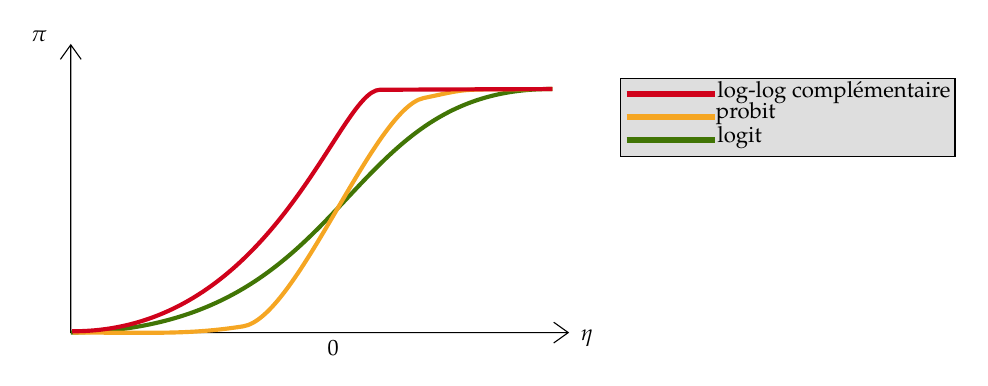
\begin{tikzpicture}[x=0.75pt,y=0.75pt,yscale=-1,xscale=1]
%uncomment if require: \path (0,300); %set diagram left start at 0, and has height of 300

%Shape: Axis 2D [id:dp48000806956401476] 
\draw  (98.17,148.64) -- (338.17,148.64)(98.5,10) -- (98.5,148.64) (331.17,143.64) -- (338.17,148.64) -- (331.17,153.64) (93.5,17) -- (98.5,10) -- (103.5,17)  ;
%Curve Lines [id:da6911332547105664] 
\draw [color={rgb, 255:red, 65; green, 117; blue, 5 }  ,draw opacity=1 ][line width=1.5]    (98.5,148.64) .. controls (236.5,146.64) and (225.5,30.64) .. (330.5,31.3) ;
%Curve Lines [id:da5236167901193742] 
\draw [color={rgb, 255:red, 245; green, 166; blue, 35 }  ,draw opacity=1 ][line width=1.5]    (99.5,148.64) .. controls (139.5,148.64) and (155.5,149.64) .. (181.5,145.64) .. controls (207.5,141.64) and (244.5,40.64) .. (268.5,35.64) .. controls (292.5,30.64) and (282.5,31.64) .. (330.5,31.3) ;
%Curve Lines [id:da7105130930164139] 
\draw [color={rgb, 255:red, 208; green, 2; blue, 27 }  ,draw opacity=1 ][line width=1.5]    (99.17,148) .. controls (196.5,148.3) and (227.5,31.64) .. (247.5,31.64) .. controls (267.5,31.64) and (231.5,31.64) .. (330.5,31.3) ;
%Shape: Rectangle [id:dp3994976422081038] 
\draw  [fill={rgb, 255:red, 222; green, 222; blue, 222 }  ,fill opacity=1 ] (363.54,26.08) -- (524.5,26.08) -- (524.5,63.64) -- (363.54,63.64) -- cycle ;
%Straight Lines [id:da8147114892565948] 
\draw [color={rgb, 255:red, 208; green, 2; blue, 27 }  ,draw opacity=1 ][line width=2.25]    (366.27,33.85) -- (408.99,33.85) ;
%Straight Lines [id:da8363691109245619] 
\draw [color={rgb, 255:red, 245; green, 166; blue, 35 }  ,draw opacity=1 ][line width=2.25]    (366.27,44.85) -- (408.99,44.85) ;
%Straight Lines [id:da07649571164976332] 
\draw [color={rgb, 255:red, 65; green, 117; blue, 5 }  ,draw opacity=1 ][line width=2.25]    (366.27,55.86) -- (408.99,55.86) ;

% Text Node
\draw (466.22,32.77) node  [font=\small] [align=left] {{\footnotesize log-log complémentaire}};
% Text Node
\draw (423.72,43.27) node  [font=\small] [align=left] {{\footnotesize probit}};
% Text Node
\draw (420.72,54.77) node  [font=\small] [align=left] {{\footnotesize logit}};
% Text Node
\draw (343,146) node [anchor=north west][inner sep=0.75pt]   [align=left] {{\footnotesize $\displaystyle \eta $}};
% Text Node
\draw (78,2) node [anchor=north west][inner sep=0.75pt]   [align=left] {{\footnotesize $\displaystyle \pi $}};
% Text Node
\draw (221,151) node [anchor=north west][inner sep=0.75pt]   [align=left] {{\footnotesize $\displaystyle 0$}};


\end{tikzpicture}

\end{center}

\paragraph{Note}	La cote, alias le \og \textit{odds ratio} \fg{}, est \lfbox[formula]{$\frac{\pi}{1	-	\pi}$}.


\subsection{Nominal}
On suppose qu'il y a $J$ catégories possibles pour la variable réponse. 
Pour modéliser avec la régression logistique, on :
\begin{enumerate}[label	=	\circled{\arabic*}{lightgray}]
	\item	Choisit une catégorie comme catégorie de base $1$.
	\item	Pour chacune des autres catégories, on trouve les cotes relatives (\og \textit{relative odds} \fg{}).
\end{enumerate}

Le logarithme de la cote de la catégorie $j$ relatif à la catégorie de base $1$ est :
\begin{align*}
	\ln \frac{\pi_{j}}{\pi_{1}}
	&=	\sum_{i	=	1}^{p} \beta_{ij} X_{i}
	=	\eta_{j}, \quad j	=	2, 3, \dots, J
\end{align*}

Alors, $\pi_{j}	=	\pi_{1}\textrm{e}^{\eta_{j}}$ et puisque les probabilités doivent sommer jusqu'à 1 :
\begin{align*}
	\pi_{1}
	&=	\frac{1}{1 + \sum_{k	=	2}^{J} \textrm{e}^{\eta_{k}}}	\\
	\pi_{j}
	&=	\frac{\textrm{e}^{\eta_{j}}}{1 + \sum_{k	=	2}^{J} \textrm{e}^{\eta_{k}}}, \quad j	=	2, 3, \dots, J
\end{align*}


\subsection{Ordinal}
\textbf{Modèle logit cumulatif}

\begin{align*}
	\frac{\Pr(Y \leq j)}{1	-	\Pr(Y \leq j)}
	&=	\frac{\sum_{k	=	1}^{j} \pi_{k}}{1	-	\sum_{k	=	1}^{j} \pi_{k}}	
	=	\frac{\pi_{1} + \hdots + \pi_{j}}{\pi_{j + 1} + \hdots + \pi_{J}}	\\
\end{align*}

Alors, avec les paramètres $\beta$ qui varient par catégorie $j$, :
\begin{align*}
	\ln\left(\frac{\pi_{1} + \hdots + \pi_{j}}{\pi_{j + 1} + \hdots + \pi_{J}}\right)
	&=	\sum_{i	=	1}^{p}\beta_{ij}X_{i}	\\
\end{align*}

\textbf{Modèle de cotes proportionnelles}	\\
Excepté l'intercepte, les paramètres $\beta$ ne varient pas par catégorie $j$ :
\begin{align*}
	\ln\left(\frac{\pi_{1} + \hdots + \pi_{j}}{\pi_{j + 1} + \hdots + \pi_{J}}\right)
	&=	\beta_{1j} + \sum_{i	=	2}^{p}\beta_{i}X_{i}	\\
\end{align*}

\textbf{Modèle logit de catégories adjacentes}
\begin{align*}
	\ln\left(\frac{\pi_{j}}{\pi_{j + 1}}\right)
	&=	\sum_{i	=	1}^{p}\beta_{ij}X_{i}	\\
\end{align*}

\textbf{Modèle logit de ratio continu}
\begin{align*}
	\frac{\Pr(Y	=	j)}{\Pr(Y	>	j)}
	&=	\frac{\pi_{j}}{\pi_{j + 1} + \hdots + \pi_{J}}
\end{align*}


\pagebreak
\section{Autres}
%	https://www.youtube.com/watch?v=0XfXHYDYoBA
\begin{tabular}{|	c	|	c	|}
Régression	&	Type de variable réponse	\\\hline
Linéaire		&	Continue	\\
Logistique	&	Binaire	\\
Poisson		&	Données de comptage	\\
Analyse de survie	&	Temps jusqu'à un événement	\\
\end{tabular}
\begin{itemize}
	\item	Logistique prédit la probabilité qu'un événement ait lieu.
	\item	Poisson prédit le \og \textit{rate} \fg{} auquel des événements aient lieu.
		\begin{itemize}
		\item	C'est-à-dire, le nombre de fois, ou la fréquence, d'un événement sur une période de temps.
		\item	Donc, le temps est fixé et on observe le nombre d'événements.
		\item	On ne peut pas simplement appliquer un modèle linéaire, car les données suivent une distribution de Poisson, pas une distribution normale! 
		\item	Également, nous pouvons modéliser un \og \textit{offset} \fg{} pour considérer le temps d'exposition.
		\end{itemize}
	\item	Avec l'analyse de survie, on prédit le temps avant qu'un événement ait lieu.
		\begin{itemize}
		\item	Donc, le nombre d'événements est fixé à un et on veut savoir le temps avant qu'il ait lieu.
		\end{itemize}
\end{itemize}

\subsubsection{Poisson}
Il y a plusieurs façons de modéliser un même modèle de Poisson : 
\begin{enumerate}
	\item	Modéliser le taux comme une fonction log-linéaire des $x$ : $\lambda	=	\textrm{e}^{\beta_{0} + \beta_{1}x_{1} + \dots + \beta_{p}x_{p}}$.
		\begin{itemize}
		\item	Ceci puisque le taux $\lambda$ a une forme exponentielle.
		\end{itemize}
	\item	Modéliser le log du taux comme une fonction linéaire des $x$ : $\ln(\lambda)	=	\beta_{0} + \beta_{1}x_{1} + \dots + \beta_{p}x_{p}$.
		\begin{itemize}
		\item	Ceci permet de traiter le taux $\lambda$ avec un modèle linéaire.
		\item	L'avantage est la simplicité d'une ligne pour résumer le modèle.
		\item	Mathématiquement, les deux premières équations sont équivalentes.
		\end{itemize}
	\item	Modéliser le log de la fréquence espérée avec un \og \textit{offset} \fg{} : $\ln(\text{E}[Y])	=	\ln(\text{E}[\lambda t])	=	\beta_{0} + \beta_{1}x_{1} + \dots + \beta_{p}x_{p}	+	\ln(t)$.
		\begin{itemize}
		\item	La deuxième équation représente ce que l'on fait en théorie alors que la troisième représente ce que l'on fait en pratique.
		\end{itemize}
\end{enumerate}

Hypothèses du modèle :
\begin{enumerate}
	\item	Les observations sont indépendantes.
		\begin{itemize}
		\item	Si, par exemple, avoir une récidive augmente la probabilité d'une deuxième récidive, alors le modèle n'est pas adéquat.
		\end{itemize}
	\item	Le taux auquel les événements se produisent est une fonction log-linéaire de $x$.
		\begin{itemize}
		\item	C'est-à-dire, le log du taux est une fonction linéaire des $x$.
		\end{itemize}
	\item	Les variations dans les $x$'s ont des effets multiplicatifs sur le nombre d'événements.
		\begin{itemize}
		\item	Par exemple, si on modélise la fréquence d'accidents auto alors on s'attend à ce que le nombre d'accidents sur deux ans soit le double du nombre d'accidents sur un an.
		\end{itemize}
	\item	La moyenne = variance = $\lambda$.
	\item	Le taux est constant.
		\begin{itemize}
		\item	Donc, on pose que le taux est fixe.
		\item	Par exemple, la probabilité d'une récidive pourrait diminuer dans le temps.
		\end{itemize}
\end{enumerate}

Le modèle à deux gros problèmes, \underline{premièrement} la \textbf{sur-dispersion} où la variance est supérieure à la moyenne.
\begin{itemize}
		\item	C'est-à-dire que les données sont plus variables que ce qui est attendu.
		\item	Contrairement à la régression linéaire où l'estimation de la moyenne et du SSE est séparée, l'estimation est la même pour le modèle de Poisson.
		\item	Il y a des multiples raisons pour lesquelles ceci peut arriver : 
			\begin{enumerate}
			\item	Nous n'avons pas inclus toutes les variables explicatives significatives dans le modèle.
			\item	La forme fonctionnelle du modèle est inadéquate (p. ex., les données ne sont pas log linéaires).
			\item	Une variable est supposée d'être homogène alors qu'elle ne l'est pas.
				\begin{itemize}
				\item	P. ex., modéliser un groupe de fumeurs alors qu'il y a des sous-groupes (ceux qui font de l'exercice vs ceux qui n'en font pas, etc.)
				\end{itemize}
			\item	etc.
			\end{enumerate}
\end{itemize}

On peut calculer la \textbf{dispersion} et on désire qu'elle soit environ de 1.\\
Pour résoudre la sur-dispersion, on peut : 
\begin{enumerate}
	\item	On peut pondérer l'erreur type de tous les coefficients par la racine du paramètre de dispersion.
		\begin{itemize}
		\item	Ceci ne change pas les prévisions, plutôt ça augmente l'erreur type pour tenir compte du fait que la variabilité des données observées est plus élevée que ce à quoi on s'attendait.
		\end{itemize}
	\item	On peut ajuster un modèle avec une distribution binomiale négative.
		\begin{itemize}
		\item	Ceci permet d'estimer la fréquence et la variance séparément.
		\item	La variance sera plus grande, mais proportionnelle à la moyenne.
		\end{itemize}
\end{enumerate}


\underline{Deuxièmement}, \textbf{Données gonflées à zéro}. 
\begin{itemize}
	\item	L'idée est de modéliser la probabilité que l'événement ait lieu ou pas séparément de la fréquence.
	\item	On peut modéliser la probabilité avec un modèle logistique est la fréquence avec un modèle de Poisson.
\end{itemize}




\textbf{Matrice de confusion : }
\begin{center}


\tikzset{every picture/.style={line width=0.75pt}} %set default line width to 0.75pt        

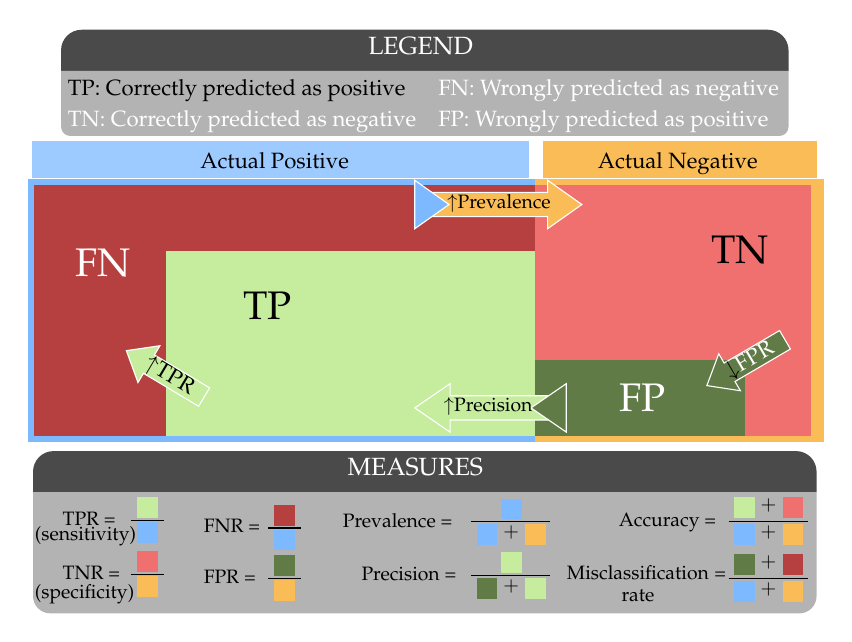
\begin{tikzpicture}[x=0.75pt,y=0.75pt,yscale=-1,xscale=1]
%uncomment if require: \path (0,366); %set diagram left start at 0, and has height of 366

%Rounded Same Side Corner Rect [id:dp5863189014777732] 
\draw  [draw opacity=0][fill={rgb, 255:red, 74; green, 74; blue, 74 }  ,fill opacity=1 ][line width=1.5]  (186.37,215.03) .. controls (186.37,209.57) and (190.8,205.14) .. (196.27,205.14) -- (553.98,205.14) .. controls (559.45,205.14) and (563.87,209.57) .. (563.87,215.03) -- (563.87,224.92) .. controls (563.87,224.92) and (563.87,224.92) .. (563.87,224.92) -- (186.37,224.92) .. controls (186.37,224.92) and (186.37,224.92) .. (186.37,224.92) -- cycle ;
%Rounded Same Side Corner Rect [id:dp10542736831068278] 
\draw  [draw opacity=0][fill={rgb, 255:red, 179; green, 179; blue, 179 }  ,fill opacity=1 ] (563.87,275.01) .. controls (563.87,279.61) and (560.15,283.33) .. (555.56,283.33) -- (194.69,283.33) .. controls (190.1,283.33) and (186.37,279.61) .. (186.37,275.01) -- (186.37,224.92) .. controls (186.37,224.92) and (186.37,224.92) .. (186.37,224.92) -- (563.87,224.92) .. controls (563.87,224.92) and (563.87,224.92) .. (563.87,224.92) -- cycle ;
%Flowchart: Process [id:dp2781782458228159] 
\draw  [draw opacity=0][fill={rgb, 255:red, 198; green, 237; blue, 158 }  ,fill opacity=1 ] (236.54,237.33) -- (246.54,237.33) -- (246.54,227.33) -- (236.54,227.33) -- cycle ;
%Flowchart: Process [id:dp6595006333689621] 
\draw  [draw opacity=0][fill={rgb, 255:red, 125; green, 185; blue, 255 }  ,fill opacity=1 ] (236.54,249.33) -- (246.54,249.33) -- (246.54,239.33) -- (236.54,239.33) -- cycle ;
%Straight Lines [id:da005645386209309766] 
\draw    (233.54,238.5) -- (249.54,238.5) ;

%Flowchart: Process [id:dp7524991543129134] 
\draw  [draw opacity=0][fill={rgb, 255:red, 125; green, 185; blue, 255 }  ,fill opacity=1 ] (302.54,253) -- (312.54,253) -- (312.54,243) -- (302.54,243) -- cycle ;
%Straight Lines [id:da5176971400521515] 
\draw    (299.54,242.17) -- (315.54,242.17) ;
%Flowchart: Process [id:dp9574550023533219] 
\draw  [draw opacity=0][fill={rgb, 255:red, 182; green, 64; blue, 64 }  ,fill opacity=1 ] (302.54,241) -- (312.54,241) -- (312.54,231) -- (302.54,231) -- cycle ;

%Flowchart: Process [id:dp6446573608226225] 
\draw  [draw opacity=0][fill={rgb, 255:red, 240; green, 111; blue, 111 }  ,fill opacity=1 ] (236.54,263.5) -- (246.54,263.5) -- (246.54,253.5) -- (236.54,253.5) -- cycle ;
%Flowchart: Process [id:dp6670926329350344] 
\draw  [draw opacity=0][fill={rgb, 255:red, 249; green, 188; blue, 87 }  ,fill opacity=1 ] (236.54,275.5) -- (246.54,275.5) -- (246.54,265.5) -- (236.54,265.5) -- cycle ;
%Straight Lines [id:da5832941059999399] 
\draw    (233.54,264.67) -- (249.54,264.67) ;

%Flowchart: Process [id:dp3885928458657999] 
\draw  [draw opacity=0][fill={rgb, 255:red, 249; green, 188; blue, 87 }  ,fill opacity=1 ] (302.54,277.33) -- (312.54,277.33) -- (312.54,267.33) -- (302.54,267.33) -- cycle ;
%Straight Lines [id:da3401710446338324] 
\draw    (299.54,266.5) -- (315.54,266.5) ;
%Flowchart: Process [id:dp6813365938208455] 
\draw  [draw opacity=0][fill={rgb, 255:red, 97; green, 123; blue, 71 }  ,fill opacity=1 ] (302.54,265.33) -- (312.54,265.33) -- (312.54,255.33) -- (302.54,255.33) -- cycle ;

%Flowchart: Process [id:dp26333217881412674] 
\draw  [draw opacity=0][fill={rgb, 255:red, 198; green, 237; blue, 158 }  ,fill opacity=1 ] (412.04,263.83) -- (422.04,263.83) -- (422.04,253.83) -- (412.04,253.83) -- cycle ;
%Flowchart: Process [id:dp33935301348671065] 
\draw  [draw opacity=0][fill={rgb, 255:red, 97; green, 123; blue, 71 }  ,fill opacity=1 ] (400.04,276.33) -- (410.04,276.33) -- (410.04,266.33) -- (400.04,266.33) -- cycle ;
%Straight Lines [id:da4578404875999813] 
\draw    (397.54,265) -- (435.54,265) ;
%Flowchart: Process [id:dp07704188689930547] 
\draw  [draw opacity=0][fill={rgb, 255:red, 198; green, 237; blue, 158 }  ,fill opacity=1 ] (423.54,276.33) -- (433.54,276.33) -- (433.54,266.33) -- (423.54,266.33) -- cycle ;

%Flowchart: Process [id:dp511192763925254] 
\draw  [draw opacity=0][fill={rgb, 255:red, 125; green, 185; blue, 255 }  ,fill opacity=1 ] (412.04,238) -- (422.04,238) -- (422.04,228) -- (412.04,228) -- cycle ;
%Flowchart: Process [id:dp8487027222224734] 
\draw  [draw opacity=0][fill={rgb, 255:red, 125; green, 185; blue, 255 }  ,fill opacity=1 ] (400.04,250.5) -- (410.04,250.5) -- (410.04,240.5) -- (400.04,240.5) -- cycle ;
%Straight Lines [id:da11748805900160852] 
\draw    (397.54,239.17) -- (435.54,239.17) ;
%Flowchart: Process [id:dp6757535243694623] 
\draw  [draw opacity=0][fill={rgb, 255:red, 249; green, 188; blue, 87 }  ,fill opacity=1 ] (423.54,250.5) -- (433.54,250.5) -- (433.54,240.5) -- (423.54,240.5) -- cycle ;

%Flowchart: Process [id:dp23257062904433523] 
\draw  [draw opacity=0][fill={rgb, 255:red, 125; green, 185; blue, 255 }  ,fill opacity=1 ] (524.04,250.5) -- (534.04,250.5) -- (534.04,240.5) -- (524.04,240.5) -- cycle ;
%Straight Lines [id:da16879793480007654] 
\draw    (521.54,239.17) -- (559.54,239.17) ;
%Flowchart: Process [id:dp629293047660624] 
\draw  [draw opacity=0][fill={rgb, 255:red, 249; green, 188; blue, 87 }  ,fill opacity=1 ] (547.54,250.5) -- (557.54,250.5) -- (557.54,240.5) -- (547.54,240.5) -- cycle ;
%Flowchart: Process [id:dp25903639593069716] 
\draw  [draw opacity=0][fill={rgb, 255:red, 198; green, 237; blue, 158 }  ,fill opacity=1 ] (524.04,237.5) -- (534.04,237.5) -- (534.04,227.5) -- (524.04,227.5) -- cycle ;
%Flowchart: Process [id:dp2784202862814029] 
\draw  [draw opacity=0][fill={rgb, 255:red, 240; green, 111; blue, 111 }  ,fill opacity=1 ] (547.54,237.5) -- (557.54,237.5) -- (557.54,227.5) -- (547.54,227.5) -- cycle ;

%Flowchart: Process [id:dp5706215732887201] 
\draw  [draw opacity=0][fill={rgb, 255:red, 125; green, 185; blue, 255 }  ,fill opacity=1 ] (524.04,277.83) -- (534.04,277.83) -- (534.04,267.83) -- (524.04,267.83) -- cycle ;
%Straight Lines [id:da24052635124853383] 
\draw    (521.54,266.5) -- (559.54,266.5) ;
%Flowchart: Process [id:dp8806206355646873] 
\draw  [draw opacity=0][fill={rgb, 255:red, 249; green, 188; blue, 87 }  ,fill opacity=1 ] (547.54,277.83) -- (557.54,277.83) -- (557.54,267.83) -- (547.54,267.83) -- cycle ;
%Flowchart: Process [id:dp025661689438194246] 
\draw  [draw opacity=0][fill={rgb, 255:red, 97; green, 123; blue, 71 }  ,fill opacity=1 ] (524.04,264.83) -- (534.04,264.83) -- (534.04,254.83) -- (524.04,254.83) -- cycle ;
%Flowchart: Process [id:dp07416724651822326] 
\draw  [draw opacity=0][fill={rgb, 255:red, 182; green, 64; blue, 64 }  ,fill opacity=1 ] (547.54,264.83) -- (557.54,264.83) -- (557.54,254.83) -- (547.54,254.83) -- cycle ;


%Shape: Rectangle [id:dp9078887636984747] 
\draw  [color={rgb, 255:red, 125; green, 185; blue, 255 }  ,draw opacity=1 ][fill={rgb, 255:red, 125; green, 185; blue, 255 }  ,fill opacity=1 ][line width=4.5]  (186.79,76.98) -- (428.29,76.98) -- (428.29,198) -- (186.79,198) -- cycle ;
%Shape: Rectangle [id:dp6719473196737591] 
\draw  [color={rgb, 255:red, 249; green, 188; blue, 87 }  ,draw opacity=1 ][fill={rgb, 255:red, 249; green, 188; blue, 87 }  ,fill opacity=1 ][line width=4.5]  (431.29,76.98) -- (564.29,76.98) -- (564.29,198) -- (431.29,198) -- cycle ;
%Shape: Rectangle [id:dp8554811027992568] 
\draw  [draw opacity=0][fill={rgb, 255:red, 240; green, 111; blue, 111 }  ,fill opacity=1 ][line width=0.75]  (427.96,76.98) -- (560.96,76.98) -- (560.96,198) -- (427.96,198) -- cycle ;
%Shape: Rectangle [id:dp4666790964474916] 
\draw  [draw opacity=0][fill={rgb, 255:red, 182; green, 64; blue, 64 }  ,fill opacity=1 ] (186.79,76.98) -- (428.29,76.98) -- (428.29,198) -- (186.79,198) -- cycle ;
%Shape: Rectangle [id:dp4684932062372884] 
\draw  [draw opacity=0][fill={rgb, 255:red, 125; green, 185; blue, 255 }  ,fill opacity=0.75 ] (185.96,55.67) -- (425.29,55.67) -- (425.29,73.33) -- (185.96,73.33) -- cycle ;
%Shape: Rectangle [id:dp7538608016518991] 
\draw  [draw opacity=0][fill={rgb, 255:red, 249; green, 188; blue, 87 }  ,fill opacity=1 ] (432.29,55.67) -- (563.96,55.67) -- (563.96,73.33) -- (432.29,73.33) -- cycle ;
%Shape: Rectangle [id:dp575388567694743] 
\draw  [draw opacity=0][fill={rgb, 255:red, 198; green, 237; blue, 158 }  ,fill opacity=1 ] (250.29,108.8) -- (428.29,108.8) -- (428.29,198) -- (250.29,198) -- cycle ;
%Shape: Rectangle [id:dp694025502587706] 
\draw  [draw opacity=0][fill={rgb, 255:red, 97; green, 123; blue, 71 }  ,fill opacity=1 ] (428.29,161.33) -- (529.29,161.33) -- (529.29,198) -- (428.29,198) -- cycle ;
%Left Arrow [id:dp159442790435544] 
\draw  [color={rgb, 255:red, 255; green, 255; blue, 255 }  ,draw opacity=1 ][fill={rgb, 255:red, 97; green, 123; blue, 71 }  ,fill opacity=1 ] (511.02,173.58) -- (516.74,158.26) -- (519.35,162.71) -- (546.06,147.06) -- (551.28,155.96) -- (524.57,171.61) -- (527.18,176.07) -- cycle ;

%Left Arrow [id:dp2567253964557259] 
\draw  [color={rgb, 255:red, 255; green, 255; blue, 255 }  ,draw opacity=1 ][fill={rgb, 255:red, 198; green, 237; blue, 158 }  ,fill opacity=1 ] (231.33,156.74) -- (247.51,154.38) -- (244.87,158.81) -- (271.45,174.68) -- (266.16,183.54) -- (239.58,167.67) -- (236.93,172.1) -- cycle ;

%Left Arrow [id:dp4712888920317464] 
\draw  [color={rgb, 255:red, 255; green, 255; blue, 255 }  ,draw opacity=1 ][fill={rgb, 255:red, 198; green, 237; blue, 158 }  ,fill opacity=1 ] (370.29,184.33) -- (387.29,172.66) -- (387.29,178.5) -- (440.29,178.5) -- (440.29,190.17) -- (387.29,190.17) -- (387.29,196) -- cycle ;
%Left Arrow [id:dp3521145387427629] 
\draw  [color={rgb, 255:red, 255; green, 255; blue, 255 }  ,draw opacity=1 ][fill={rgb, 255:red, 97; green, 123; blue, 71 }  ,fill opacity=1 ] (426.29,184.33) -- (443.29,172.66) -- (443.29,178.5) -- (443.29,178.5) -- (443.29,190.17) -- (443.29,190.17) -- (443.29,196) -- cycle ;

%Left Arrow [id:dp8166384807624658] 
\draw  [color={rgb, 255:red, 255; green, 255; blue, 255 }  ,draw opacity=1 ][fill={rgb, 255:red, 249; green, 188; blue, 87 }  ,fill opacity=1 ] (450.8,86.33) -- (434.29,74.66) -- (434.29,80.5) -- (370.29,80.5) -- (370.29,92.17) -- (434.29,92.17) -- (434.29,98) -- cycle ;
%Left Arrow [id:dp8194414952038565] 
\draw  [color={rgb, 255:red, 255; green, 255; blue, 255 }  ,draw opacity=1 ][fill={rgb, 255:red, 125; green, 185; blue, 255 }  ,fill opacity=1 ] (386.8,86.33) -- (370.29,74.66) -- (370.29,80.5) -- (370.29,80.5) -- (370.29,92.17) -- (370.29,92.17) -- (370.29,98) -- cycle ;


%Rounded Same Side Corner Rect [id:dp01839882980964913] 
\draw  [draw opacity=0][fill={rgb, 255:red, 74; green, 74; blue, 74 }  ,fill opacity=1 ][line width=1.5]  (199.87,12.03) .. controls (199.87,6.57) and (204.3,2.14) .. (209.77,2.14) -- (540.48,2.14) .. controls (545.95,2.14) and (550.37,6.57) .. (550.37,12.03) -- (550.37,21.92) .. controls (550.37,21.92) and (550.37,21.92) .. (550.37,21.92) -- (199.87,21.92) .. controls (199.87,21.92) and (199.87,21.92) .. (199.87,21.92) -- cycle ;
%Rounded Same Side Corner Rect [id:dp42232070994654003] 
\draw  [draw opacity=0][fill={rgb, 255:red, 179; green, 179; blue, 179 }  ,fill opacity=1 ] (550.37,48.86) .. controls (550.37,51.33) and (548.37,53.33) .. (545.9,53.33) -- (204.35,53.33) .. controls (201.88,53.33) and (199.87,51.33) .. (199.87,48.86) -- (199.87,21.92) .. controls (199.87,21.92) and (199.87,21.92) .. (199.87,21.92) -- (550.37,21.92) .. controls (550.37,21.92) and (550.37,21.92) .. (550.37,21.92) -- cycle ;


% Text Node
\draw (267.37,236.67) node [anchor=north west][inner sep=0.75pt]  [font=\scriptsize] [align=left] {FNR = };
% Text Node
\draw (267.37,261) node [anchor=north west][inner sep=0.75pt]  [font=\scriptsize] [align=left] {FPR = };
% Text Node
\draw (343.37,259.5) node [anchor=north west][inner sep=0.75pt]  [font=\scriptsize] [align=left] {Precision = };
% Text Node
\draw (411.54,265.83) node [anchor=north west][inner sep=0.75pt]  [font=\scriptsize] [align=left] {$\displaystyle +$};
% Text Node
\draw (535.54,267.33) node [anchor=north west][inner sep=0.75pt]  [font=\scriptsize] [align=left] {$\displaystyle +$};
% Text Node
\draw (440.37,259) node [anchor=north west][inner sep=0.75pt]  [font=\scriptsize] [align=left] {\begin{minipage}[lt]{54.30085600000001pt}\setlength\topsep{0pt}
\begin{center}
Misclassification\\rate 
\end{center}

\end{minipage}};
% Text Node
\draw (535.54,254.33) node [anchor=north west][inner sep=0.75pt]  [font=\scriptsize] [align=left] {$\displaystyle +$};
% Text Node
\draw (513.37,262) node [anchor=north west][inner sep=0.75pt]  [font=\scriptsize] [align=left] {= };
% Text Node
\draw (535.54,240) node [anchor=north west][inner sep=0.75pt]  [font=\scriptsize] [align=left] {$\displaystyle +$};
% Text Node
\draw (467.37,233.67) node [anchor=north west][inner sep=0.75pt]  [font=\scriptsize] [align=left] {Accuracy = };
% Text Node
\draw (535.54,227) node [anchor=north west][inner sep=0.75pt]  [font=\scriptsize] [align=left] {$\displaystyle +$};
% Text Node
\draw (334.37,233.67) node [anchor=north west][inner sep=0.75pt]  [font=\scriptsize] [align=left] {Prevalence = };
% Text Node
\draw (411.54,240) node [anchor=north west][inner sep=0.75pt]  [font=\scriptsize] [align=left] {$\displaystyle +$};
% Text Node
\draw (243.09,156.56) node [anchor=north west][inner sep=0.75pt]  [font=\scriptsize,rotate=-30.84] [align=left] {{\footnotesize $\displaystyle \uparrow $TPR}};
% Text Node
\draw (516.52,163.19) node [anchor=north west][inner sep=0.75pt]  [font=\scriptsize,rotate=-329.62] [align=left] {{\footnotesize $\displaystyle \downarrow $\textcolor[rgb]{1,1,1}{FPR}}};
% Text Node
\draw (382.95,178.25) node [anchor=north west][inner sep=0.75pt]  [font=\scriptsize] [align=left] {{\scriptsize $\displaystyle \uparrow $Precision}};
% Text Node
\draw (384.63,80.25) node [anchor=north west][inner sep=0.75pt]  [font=\scriptsize] [align=left] {{\scriptsize $\displaystyle \uparrow $Prevalence}};
% Text Node
\draw (199.37,233) node [anchor=north west][inner sep=0.75pt]  [font=\scriptsize] [align=left] {TPR = };
% Text Node
\draw (186,240) node [anchor=north west][inner sep=0.75pt]  [font=\scriptsize] [align=left] {{\scriptsize (sensitivity)}};
% Text Node
\draw (199.37,259.17) node [anchor=north west][inner sep=0.75pt]  [font=\scriptsize] [align=left] {TNR = };
% Text Node
\draw (186,268.17) node [anchor=north west][inner sep=0.75pt]  [font=\scriptsize] [align=left] {{\scriptsize (specificity)}};
% Text Node
\draw (264.04,60.17) node [anchor=north west][inner sep=0.75pt]  [font=\footnotesize,color={rgb, 255:red, 0; green, 0; blue, 0 }  ,opacity=1 ] [align=left] {\begin{minipage}[lt]{56.241644pt}\setlength\topsep{0pt}
\begin{center}
Actual Positive
\end{center}

\end{minipage}};
% Text Node
\draw (455.79,60.17) node [anchor=north west][inner sep=0.75pt]  [font=\footnotesize,color={rgb, 255:red, 0; green, 0; blue, 0 }  ,opacity=1 ] [align=left] {\begin{minipage}[lt]{59.875428pt}\setlength\topsep{0pt}
\begin{center}
Actual Negative
\end{center}

\end{minipage}};
% Text Node
\draw (464.29,171.17) node [anchor=north west][inner sep=0.75pt]  [font=\Large,color={rgb, 255:red, 255; green, 255; blue, 255 }  ,opacity=1 ] [align=left] {\begin{minipage}[lt]{21.490856pt}\setlength\topsep{0pt}
\begin{center}\textcolor{white}{
FP}
\end{center}

\end{minipage}};
% Text Node
\draw (204.04,106.17) node [anchor=north west][inner sep=0.75pt]  [font=\Large,color={rgb, 255:red, 255; green, 255; blue, 255 }  ,opacity=1 ] [align=left] {\begin{minipage}[lt]{22.305428000000003pt}\setlength\topsep{0pt}
\begin{center}\textcolor{white}{
FN}
\end{center}

\end{minipage}};
% Text Node
\draw (510.96,99.99) node [anchor=north west][inner sep=0.75pt]  [font=\Large,color={rgb, 255:red, 0; green, 0; blue, 0 }  ,opacity=1 ] [align=left] {\begin{minipage}[lt]{22.305428000000003pt}\setlength\topsep{0pt}
\begin{center}
TN
\end{center}

\end{minipage}};
% Text Node
\draw (283.79,126.9) node [anchor=north west][inner sep=0.75pt]  [font=\Large,color={rgb, 255:red, 0; green, 0; blue, 0 }  ,opacity=1 ] [align=left] {\begin{minipage}[lt]{21.490856pt}\setlength\topsep{0pt}
\begin{center}
TP
\end{center}

\end{minipage}};
% Text Node
\draw (336.62,207.19) node [anchor=north west][inner sep=0.75pt]  [font=\small,color={rgb, 255:red, 255; green, 255; blue, 255 }  ,opacity=1 ] [align=left] {MEASURES};
% Text Node
\draw (346.62,4.53) node [anchor=north west][inner sep=0.75pt]  [font=\small,color={rgb, 255:red, 255; green, 255; blue, 255 }  ,opacity=1 ] [align=left] {LEGEND};
% Text Node
\draw (201.87,24.92) node [anchor=north west][inner sep=0.75pt]  [font=\small,color={rgb, 255:red, 255; green, 255; blue, 255 }  ,opacity=1 ] [align=left] {{\footnotesize \textcolor[rgb]{0,0,0}{TP: Correctly predicted as positive}}\\{\footnotesize TN: Correctly predicted as negative}};
% Text Node
\draw (380.37,24.92) node [anchor=north west][inner sep=0.75pt]  [font=\small,color={rgb, 255:red, 255; green, 255; blue, 255 }  ,opacity=1 ] [align=left] {{\footnotesize FN: Wrongly predicted as negative}\\{\footnotesize FP: Wrongly predicted as positive}};


\end{tikzpicture}
\end{center}


\section{Erreur}

\begin{description}
	\item[Écart-type]	Mesure la variation \underline{entre les observations} d'\textbf{un} ensemble de données.
		\begin{itemize}[leftmargin = *]
		\item	\og \textit{standard deviation} \fg{}.
		\end{itemize}
		\begin{center}

\tikzset{every picture/.style={line width=0.75pt}} %set default line width to 0.75pt        

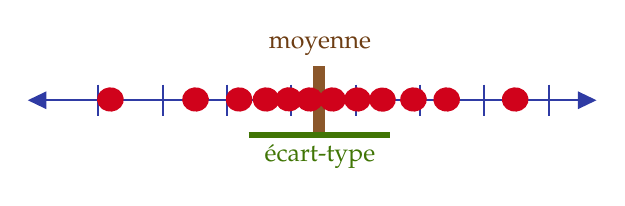
\begin{tikzpicture}[x=0.75pt,y=0.75pt,yscale=-1,xscale=1]
%uncomment if require: \path (0,174); %set diagram left start at 0, and has height of 174

%Straight Lines [id:da5554502737558269] 
\draw [color={rgb, 255:red, 47; green, 59; blue, 164 }  ,draw opacity=1 ][line width=0.75]    (279.83,38) -- (547.83,38) (310.83,30.5) -- (310.83,45.5)(341.83,30.5) -- (341.83,45.5)(372.83,30.5) -- (372.83,45.5)(403.83,30.5) -- (403.83,45.5)(434.83,30.5) -- (434.83,45.5)(465.83,30.5) -- (465.83,45.5)(496.83,30.5) -- (496.83,45.5)(527.83,30.5) -- (527.83,45.5) ;
\draw [shift={(550.83,38)}, rotate = 180] [fill={rgb, 255:red, 47; green, 59; blue, 164 }  ,fill opacity=1 ][line width=0.08]  [draw opacity=0] (8.93,-4.29) -- (0,0) -- (8.93,4.29) -- cycle    ;
\draw [shift={(276.83,38)}, rotate = 0] [fill={rgb, 255:red, 47; green, 59; blue, 164 }  ,fill opacity=1 ][line width=0.08]  [draw opacity=0] (8.93,-4.29) -- (0,0) -- (8.93,4.29) -- cycle    ;
%Straight Lines [id:da6666232383065853] 
\draw [color={rgb, 255:red, 139; green, 87; blue, 42 }  ,draw opacity=1 ][line width=2.25]    (415.67,54.92) -- (415.67,21.42)(418.67,54.92) -- (418.67,21.42) ;
%Flowchart: Connector [id:dp30389051575543746] 
\draw  [draw opacity=0][fill={rgb, 255:red, 208; green, 2; blue, 27 }  ,fill opacity=1 ] (320.71,33.09) .. controls (317.96,31.04) and (313.9,31.42) .. (311.65,33.93) .. controls (309.4,36.44) and (309.81,40.13) .. (312.57,42.17) .. controls (315.33,44.21) and (319.39,43.84) .. (321.63,41.33) .. controls (323.88,38.82) and (323.47,35.13) .. (320.71,33.09) -- cycle ;
%Flowchart: Connector [id:dp8054636909486927] 
\draw  [draw opacity=0][fill={rgb, 255:red, 208; green, 2; blue, 27 }  ,fill opacity=1 ] (382.71,33.09) .. controls (379.96,31.04) and (375.9,31.42) .. (373.65,33.93) .. controls (371.4,36.44) and (371.81,40.13) .. (374.57,42.17) .. controls (377.33,44.21) and (381.39,43.84) .. (383.63,41.33) .. controls (385.88,38.82) and (385.47,35.13) .. (382.71,33.09) -- cycle ;
%Flowchart: Connector [id:dp4481822183684774] 
\draw  [draw opacity=0][fill={rgb, 255:red, 208; green, 2; blue, 27 }  ,fill opacity=1 ] (361.71,33.09) .. controls (358.96,31.04) and (354.9,31.42) .. (352.65,33.93) .. controls (350.4,36.44) and (350.81,40.13) .. (353.57,42.17) .. controls (356.33,44.21) and (360.39,43.84) .. (362.63,41.33) .. controls (364.88,38.82) and (364.47,35.13) .. (361.71,33.09) -- cycle ;
%Flowchart: Connector [id:dp9320426369464008] 
\draw  [draw opacity=0][fill={rgb, 255:red, 208; green, 2; blue, 27 }  ,fill opacity=1 ] (416.71,33.09) .. controls (413.96,31.04) and (409.9,31.42) .. (407.65,33.93) .. controls (405.4,36.44) and (405.81,40.13) .. (408.57,42.17) .. controls (411.33,44.21) and (415.39,43.84) .. (417.63,41.33) .. controls (419.88,38.82) and (419.47,35.13) .. (416.71,33.09) -- cycle ;
%Flowchart: Connector [id:dp5645916521008547] 
\draw  [draw opacity=0][fill={rgb, 255:red, 208; green, 2; blue, 27 }  ,fill opacity=1 ] (395.71,33.09) .. controls (392.96,31.04) and (388.9,31.42) .. (386.65,33.93) .. controls (384.4,36.44) and (384.81,40.13) .. (387.57,42.17) .. controls (390.33,44.21) and (394.39,43.84) .. (396.63,41.33) .. controls (398.88,38.82) and (398.47,35.13) .. (395.71,33.09) -- cycle ;
%Flowchart: Connector [id:dp9615392127090878] 
\draw  [draw opacity=0][fill={rgb, 255:red, 208; green, 2; blue, 27 }  ,fill opacity=1 ] (439.71,33.09) .. controls (436.96,31.04) and (432.9,31.42) .. (430.65,33.93) .. controls (428.4,36.44) and (428.81,40.13) .. (431.57,42.17) .. controls (434.33,44.21) and (438.39,43.84) .. (440.63,41.33) .. controls (442.88,38.82) and (442.47,35.13) .. (439.71,33.09) -- cycle ;
%Flowchart: Connector [id:dp18343654664200626] 
\draw  [draw opacity=0][fill={rgb, 255:red, 208; green, 2; blue, 27 }  ,fill opacity=1 ] (427.71,33.09) .. controls (424.96,31.04) and (420.9,31.42) .. (418.65,33.93) .. controls (416.4,36.44) and (416.81,40.13) .. (419.57,42.17) .. controls (422.33,44.21) and (426.39,43.84) .. (428.63,41.33) .. controls (430.88,38.82) and (430.47,35.13) .. (427.71,33.09) -- cycle ;
%Flowchart: Connector [id:dp49357374316679636] 
\draw  [draw opacity=0][fill={rgb, 255:red, 208; green, 2; blue, 27 }  ,fill opacity=1 ] (466.71,33.09) .. controls (463.96,31.04) and (459.9,31.42) .. (457.65,33.93) .. controls (455.4,36.44) and (455.81,40.13) .. (458.57,42.17) .. controls (461.33,44.21) and (465.39,43.84) .. (467.63,41.33) .. controls (469.88,38.82) and (469.47,35.13) .. (466.71,33.09) -- cycle ;
%Flowchart: Connector [id:dp5732145021055151] 
\draw  [draw opacity=0][fill={rgb, 255:red, 208; green, 2; blue, 27 }  ,fill opacity=1 ] (451.78,33.16) .. controls (449.02,31.12) and (444.96,31.49) .. (442.71,34) .. controls (440.46,36.51) and (440.88,40.2) .. (443.63,42.24) .. controls (446.39,44.28) and (450.45,43.91) .. (452.7,41.4) .. controls (454.94,38.89) and (454.53,35.2) .. (451.78,33.16) -- cycle ;
%Flowchart: Connector [id:dp9989913792112952] 
\draw  [draw opacity=0][fill={rgb, 255:red, 208; green, 2; blue, 27 }  ,fill opacity=1 ] (515.71,33.09) .. controls (512.96,31.04) and (508.9,31.42) .. (506.65,33.93) .. controls (504.4,36.44) and (504.81,40.13) .. (507.57,42.17) .. controls (510.33,44.21) and (514.39,43.84) .. (516.63,41.33) .. controls (518.88,38.82) and (518.47,35.13) .. (515.71,33.09) -- cycle ;
%Flowchart: Connector [id:dp2709053942707078] 
\draw  [draw opacity=0][fill={rgb, 255:red, 208; green, 2; blue, 27 }  ,fill opacity=1 ] (482.71,33.09) .. controls (479.96,31.04) and (475.9,31.42) .. (473.65,33.93) .. controls (471.4,36.44) and (471.81,40.13) .. (474.57,42.17) .. controls (477.33,44.21) and (481.39,43.84) .. (483.63,41.33) .. controls (485.88,38.82) and (485.47,35.13) .. (482.71,33.09) -- cycle ;
%Flowchart: Connector [id:dp7446426173106822] 
\draw  [draw opacity=0][fill={rgb, 255:red, 208; green, 2; blue, 27 }  ,fill opacity=1 ] (406.65,33.02) .. controls (403.89,30.97) and (399.84,31.35) .. (397.59,33.86) .. controls (395.34,36.36) and (395.75,40.05) .. (398.51,42.1) .. controls (401.27,44.14) and (405.32,43.77) .. (407.57,41.26) .. controls (409.82,38.75) and (409.41,35.06) .. (406.65,33.02) -- cycle ;
%Straight Lines [id:da9789557877821047] 
\draw [color={rgb, 255:red, 65; green, 117; blue, 5 }  ,draw opacity=1 ][line width=2.25]    (383.17,54.92) -- (451.17,54.92) ;

% Text Node
\draw (417.58,12) node  [color={rgb, 255:red, 109; green, 61; blue, 19 }  ,opacity=1 ] [align=left] {{\small moyenne}};
% Text Node
\draw (417.58,65) node  [font=\small,color={rgb, 255:red, 109; green, 61; blue, 19 }  ,opacity=1 ] [align=left] {{\small \textcolor[rgb]{0.25,0.46,0.02}{écart-type}}};


\end{tikzpicture}
		\end{center}
	\item[Erreur type]	Mesure la variation \underline{entre les moyennes} de \textbf{plusieurs} ensembles de données.
		\begin{itemize}[leftmargin = *]
		\item	\og \textit{standard error} \fg{}.
		\end{itemize}
		\begin{center}
		

\tikzset{every picture/.style={line width=0.75pt}} %set default line width to 0.75pt        

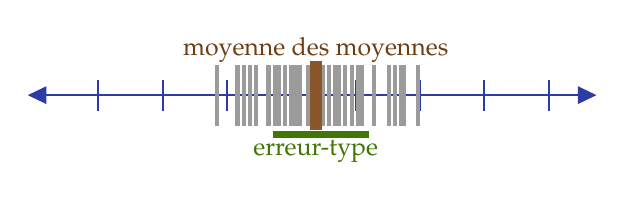
\begin{tikzpicture}[x=0.75pt,y=0.75pt,yscale=-1,xscale=1]
%uncomment if require: \path (0,174); %set diagram left start at 0, and has height of 174

%Straight Lines [id:da8220125436751056] 
\draw [color={rgb, 255:red, 47; green, 59; blue, 164 }  ,draw opacity=1 ][line width=0.75]    (281.83,118) -- (549.83,118) (312.83,110.5) -- (312.83,125.5)(343.83,110.5) -- (343.83,125.5)(374.83,110.5) -- (374.83,125.5)(405.83,110.5) -- (405.83,125.5)(436.83,110.5) -- (436.83,125.5)(467.83,110.5) -- (467.83,125.5)(498.83,110.5) -- (498.83,125.5)(529.83,110.5) -- (529.83,125.5) ;
\draw [shift={(552.83,118)}, rotate = 180] [fill={rgb, 255:red, 47; green, 59; blue, 164 }  ,fill opacity=1 ][line width=0.08]  [draw opacity=0] (8.93,-4.29) -- (0,0) -- (8.93,4.29) -- cycle    ;
\draw [shift={(278.83,118)}, rotate = 0] [fill={rgb, 255:red, 47; green, 59; blue, 164 }  ,fill opacity=1 ][line width=0.08]  [draw opacity=0] (8.93,-4.29) -- (0,0) -- (8.93,4.29) -- cycle    ;
%Straight Lines [id:da052261111869088106] 
\draw [color={rgb, 255:red, 155; green, 155; blue, 155 }  ,draw opacity=1 ][line width=1.5]    (415.83,132.67) -- (415.83,103.33) ;
%Straight Lines [id:da25533101510311673] 
\draw [color={rgb, 255:red, 155; green, 155; blue, 155 }  ,draw opacity=1 ][line width=1.5]    (420.83,132.67) -- (420.83,103.33) ;
%Straight Lines [id:da6426635244738363] 
\draw [color={rgb, 255:red, 155; green, 155; blue, 155 }  ,draw opacity=1 ][line width=1.5]    (426.83,132.67) -- (426.83,103.33) ;
%Straight Lines [id:da6924171841728055] 
\draw [color={rgb, 255:red, 155; green, 155; blue, 155 }  ,draw opacity=1 ][line width=1.5]    (423.83,132.67) -- (423.83,103.33) ;
%Straight Lines [id:da19673873838231448] 
\draw [color={rgb, 255:red, 155; green, 155; blue, 155 }  ,draw opacity=1 ][line width=1.5]    (428.83,132.67) -- (428.83,103.33) ;
%Straight Lines [id:da9733057591182157] 
\draw [color={rgb, 255:red, 155; green, 155; blue, 155 }  ,draw opacity=1 ][line width=1.5]    (434.83,132.67) -- (434.83,103.33) ;
%Straight Lines [id:da23648190125390167] 
\draw [color={rgb, 255:red, 155; green, 155; blue, 155 }  ,draw opacity=1 ][line width=1.5]    (394.83,132.67) -- (394.83,103.33) ;
%Straight Lines [id:da1303046815942539] 
\draw [color={rgb, 255:red, 155; green, 155; blue, 155 }  ,draw opacity=1 ][line width=1.5]    (399.83,132.67) -- (399.83,103.33) ;
%Straight Lines [id:da6128601437483194] 
\draw [color={rgb, 255:red, 155; green, 155; blue, 155 }  ,draw opacity=1 ][line width=1.5]    (405.83,132.67) -- (405.83,103.33) ;
%Straight Lines [id:da36533401916878416] 
\draw [color={rgb, 255:red, 155; green, 155; blue, 155 }  ,draw opacity=1 ][line width=1.5]    (402.83,132.67) -- (402.83,103.33) ;
%Straight Lines [id:da0761803178503282] 
\draw [color={rgb, 255:red, 155; green, 155; blue, 155 }  ,draw opacity=1 ][line width=1.5]    (407.83,132.67) -- (407.83,103.33) ;
%Straight Lines [id:da4536124738403875] 
\draw [color={rgb, 255:red, 155; green, 155; blue, 155 }  ,draw opacity=1 ][line width=1.5]    (413.83,132.67) -- (413.83,103.33) ;
%Straight Lines [id:da2518902010718611] 
\draw [color={rgb, 255:red, 155; green, 155; blue, 155 }  ,draw opacity=1 ][line width=1.5]    (459.83,132.67) -- (459.83,103.33) ;
%Straight Lines [id:da6762200116514319] 
\draw [color={rgb, 255:red, 155; green, 155; blue, 155 }  ,draw opacity=1 ][line width=1.5]    (452.83,132.67) -- (452.83,103.33) ;
%Straight Lines [id:da023011435062046726] 
\draw [color={rgb, 255:red, 155; green, 155; blue, 155 }  ,draw opacity=1 ][line width=1.5]    (452.83,132.67) -- (452.83,103.33) ;
%Straight Lines [id:da5498951842262785] 
\draw [color={rgb, 255:red, 155; green, 155; blue, 155 }  ,draw opacity=1 ][line width=1.5]    (458.83,132.67) -- (458.83,103.33) ;
%Straight Lines [id:da8590490011467546] 
\draw [color={rgb, 255:red, 155; green, 155; blue, 155 }  ,draw opacity=1 ][line width=1.5]    (455.83,132.67) -- (455.83,103.33) ;
%Straight Lines [id:da8877231722848657] 
\draw [color={rgb, 255:red, 155; green, 155; blue, 155 }  ,draw opacity=1 ][line width=1.5]    (466.83,132.67) -- (466.83,103.33) ;
%Straight Lines [id:da05542853037330375] 
\draw [color={rgb, 255:red, 155; green, 155; blue, 155 }  ,draw opacity=1 ][line width=1.5]    (426.83,132.67) -- (426.83,103.33) ;
%Straight Lines [id:da12451183170415692] 
\draw [color={rgb, 255:red, 155; green, 155; blue, 155 }  ,draw opacity=1 ][line width=1.5]    (431.83,132.67) -- (431.83,103.33) ;
%Straight Lines [id:da512024470962503] 
\draw [color={rgb, 255:red, 155; green, 155; blue, 155 }  ,draw opacity=1 ][line width=1.5]    (437.83,132.67) -- (437.83,103.33) ;
%Straight Lines [id:da026634526507703926] 
\draw [color={rgb, 255:red, 155; green, 155; blue, 155 }  ,draw opacity=1 ][line width=1.5]    (434.83,132.67) -- (434.83,103.33) ;
%Straight Lines [id:da04652506773140819] 
\draw [color={rgb, 255:red, 155; green, 155; blue, 155 }  ,draw opacity=1 ][line width=1.5]    (439.83,132.67) -- (439.83,103.33) ;
%Straight Lines [id:da7028504306628334] 
\draw [color={rgb, 255:red, 155; green, 155; blue, 155 }  ,draw opacity=1 ][line width=1.5]    (445.83,132.67) -- (445.83,103.33) ;
%Straight Lines [id:da3097660501000492] 
\draw [color={rgb, 255:red, 155; green, 155; blue, 155 }  ,draw opacity=1 ][line width=1.5]    (410.17,132.67) -- (410.17,103.33) ;
%Straight Lines [id:da6597565804975323] 
\draw [color={rgb, 255:red, 155; green, 155; blue, 155 }  ,draw opacity=1 ][line width=1.5]    (416.83,132.67) -- (416.83,103.33) ;
%Straight Lines [id:da9737145894752222] 
\draw [color={rgb, 255:red, 155; green, 155; blue, 155 }  ,draw opacity=1 ][line width=1.5]    (416.83,132.67) -- (416.83,103.33) ;
%Straight Lines [id:da6435581383162627] 
\draw [color={rgb, 255:red, 155; green, 155; blue, 155 }  ,draw opacity=1 ][line width=1.5]    (369.83,132.67) -- (369.83,103.33) ;
%Straight Lines [id:da02223066622835468] 
\draw [color={rgb, 255:red, 155; green, 155; blue, 155 }  ,draw opacity=1 ][line width=1.5]    (379.83,132.67) -- (379.83,103.33) ;
%Straight Lines [id:da7453774361084684] 
\draw [color={rgb, 255:red, 155; green, 155; blue, 155 }  ,draw opacity=1 ][line width=1.5]    (388.83,132.67) -- (388.83,103.33) ;
%Straight Lines [id:da06563886053491963] 
\draw [color={rgb, 255:red, 155; green, 155; blue, 155 }  ,draw opacity=1 ][line width=1.5]    (382.83,132.67) -- (382.83,103.33) ;
%Straight Lines [id:da2951853152147781] 
\draw [color={rgb, 255:red, 155; green, 155; blue, 155 }  ,draw opacity=1 ][line width=1.5]    (385.83,132.67) -- (385.83,103.33) ;
%Straight Lines [id:da10141149287438811] 
\draw [color={rgb, 255:red, 155; green, 155; blue, 155 }  ,draw opacity=1 ][line width=1.5]    (397.83,132.67) -- (397.83,103.33) ;
%Straight Lines [id:da02602036790028661] 
\draw [color={rgb, 255:red, 65; green, 117; blue, 5 }  ,draw opacity=1 ][line width=2.25]    (397.17,136.92) -- (443.17,136.92) ;
%Straight Lines [id:da5033909194183044] 
\draw [color={rgb, 255:red, 139; green, 87; blue, 42 }  ,draw opacity=1 ][line width=2.25]    (416.08,134.92) -- (416.08,101.42)(419.08,134.92) -- (419.08,101.42) ;

% Text Node
\draw (417.58,145) node  [font=\small,color={rgb, 255:red, 109; green, 61; blue, 19 }  ,opacity=1 ] [align=left] {{\small \textcolor[rgb]{0.25,0.46,0.02}{erreur-type}}};
% Text Node
\draw (417.58,96) node  [color={rgb, 255:red, 109; green, 61; blue, 19 }  ,opacity=1 ] [align=left] {{\small moyenne des moyennes}};


\end{tikzpicture}
		\end{center}
\end{description}

%\subsection{Valeurs p}
%%	https://www.youtube.com/watch?v=JQc3yx0-Q9E
%Les valeurs p ont 3 composantes:
%\begin{itemize}
%	\item	Le probabilité que la chance résulte en l'observation.
%	\item[]	e.g., probabilité d'observer 3 faces et 1 pile.
%	\item	Le probabilité d'observer quelque-chose d'autre autant rare.
%	\item[]	e.g., probabilité d'observer 3 piles et 1 face.
%	\item	Le probabilité d'observer quelque-chose d'autre encore plus rare ou plus extrême.
%	\item[]	e.g., probabilité d'observer 4 faces.
%\end{itemize}

%\section{Intervalles de confiance}

\pagebreak

\part{Mathématiques actuarielles IARD I}
\label{chapt:mathIARD}
\section{Probabilité}
\subsection{Fonctions de variables aléatoires}
\label{subsec:rvfunct}
\begin{definitionNOHFILL}[Fonction de masse de probabilité (PMF)]
Pour une variable aléatoire discrète $X$, on dénote sa fonction de masse de probabilité \lfbox[formula]{$p_{X}(x)	=	\Pr(X	=	x)$} tel que \lfbox[conditions]{$0	\leq	p(x)	\leq	1$} et \lfbox[conditions]{$\sum_{x} p(x)	=	1$}.
\end{definitionNOHFILL}

\begin{definitionNOHFILL}[Fonction de densité (PDF)]
Pour une variable aléatoire continue $X$, on dénote sa fonction de densité par $f_{X}(x)$ où \lfbox[conditions]{$f_{X}(x)	\neq	\Pr(X	=	x)$}. 
\begin{itemize}
	\item	La fonction de densité est évaluée sur des \textbf{intervalles de valeurs} pour obtenir la probabilité d'y être contenu, mais ne \textbf{représente pas une probabilité explicitement}.
\end{itemize}

De façon semblable à la PMF, \lfbox[conditions]{$f(x)	\geq	0$} et \lfbox[conditions]{$\int_{-\infty}^{\infty} f(x)dx	=	1$}.
\begin{itemize}
	\item	La différence entre les conditions pour la PMF et la PDF est que la fonction de densité peut être supérieure à $1$.
	\item	Puisqu'elle ne représente pas une probabilité, elle ne doit pas être inférieure (ou égale) à 1.
\end{itemize}
\end{definitionNOHFILL}


\begin{definitionNOHFILL}[Fonction de répartition (CDF)]
La fonction de répartition \lfbox[formula]{$F_{X}(x)	=	\Pr(X	\leq	x)$} tel que \lfbox[conditions]{$F(-\infty)	=	0$} et \lfbox[conditions]{$F(\infty)	=	1$}.

\begin{itemize}
	\item	En anglais, \og \textit{cumulative distribution function} \fg{}.
\end{itemize}
\end{definitionNOHFILL}

\begin{definitionNOHFILL}[Fonction de survie]
La fonction de survie \lfbox[formula]{$S_{X}(x)	=	\Pr(X	>	x)$} tel que \lfbox[conditions]{$S(-\infty)	=	1$} et \lfbox[conditions]{$S(\infty)	=	0$}.
\end{definitionNOHFILL}

\begin{definitionNOHFILL}[Fonction de hasard]
La fonction de hasard \lfbox[formula]{$h_{X}(x)	=	\frac{f(x)}{S(x)}$} tel que \lfbox[conditions]{$h(x)	\geq	0$}.

\begin{itemize}
	\item	Par la définition, on déduit qu'elle est \textbf{seulement applicable pour les v.a. continues}.
	\item	La fonction de hasard mesure la \textbf{vraisemblance} que la v.a. soit égale à $x$ en gonflant la PDF moins il devient vraisemblable qu'elle soit supérieure à $x$.
\end{itemize}

\begin{itemize}
	\item	En anglais, \og \textit{hazard function} \fg{}, \og \textit{hazard rate} \fg{}, \og \textit{failure rate function} \fg{} ou même \og \textit{force of mortality} \fg{}.
\end{itemize}
\end{definitionNOHFILL}

\begin{definitionNOHFILL}[Fonction de hasard cumulative]
La fonction de hasard cumulative \lfbox[formula]{$H_{X}(x)	=	\int_{-\infty}^{x}h(t)dt$}.
\begin{itemize}
	\item	Également, \lfbox[formula]{$H(x)	=	-\ln S(x)$} ou \lfbox[formula]{$S(x)	=	\textrm{e}^{-H(x)}$}.
\end{itemize}
\end{definitionNOHFILL}

\paragraph{Note}	Voir la sous-section \textit{\underline{\nameref{subsec:reliabilityVaria}}} de la section sur la \textit{\underline{\nameref{sec:reliability}}} du chapitre \textit{\underline{\nameref{chapt:varia}}} pour l'interprétation de la distribution en fonction de la fonction de hasard et de la fonction de hasard cumulative.


\columnbreak
\subsection{Moments}
Pour une v.a. $X$  \lfbox[conditions]{non-négative} et une fonction $g(x)$ tel que  \lfbox[conditions]{$g(0)	=	0$}, \lfbox[formula]{$\text{E}[g(X)]	=	\int_{0}^{\infty}g'(x) S(x)dx$}.

\begin{definitionNOHFILL}[Fonction génératrice des moments (MGF)]
La fonction génératrice des moments (MGF) d'une v.a. $X$ est dénoté comme \lfbox[formula]{$M_{X}(t)	=	\text{E}[\textrm{e}^{tX}]$}.\\

Entre autres, la MGF sert à générer les moments d'une distribution avec \lfbox[formula]{$\text{E}[X^{n}]	=	\deriv[n]{t}{M_{X}(t)}\big|_{t	=	0}$}.
\end{definitionNOHFILL}

\begin{definitionNOHFILL}[Fonction génératrice des probabilités (PGF)]
La fonction génératrice des moments (PGF) d'une v.a. $X$ est dénoté comme \lfbox[formula]{$P_{X}(t)	=	\text{E}[t^{X}]$}.\\

Entre autres, la PGF sert à :  
\begin{enumerate}
	\item	Générer les masses de probabilité d'une distribution discrète avec \lfbox[formula]{$p(n)	=	\frac{1}{n!}\deriv[n]{t}{P_{X}(t)}\big|_{t	=	0}$}.
	\item	Générer des espérances avec \lfbox[formula]{$\deriv[n]{t}{P_{X}(t)}\big|_{t	=	1}	=	\text{E}\left[X (X - 1) \hdots (X - (n - 1))\right]$}.
\end{enumerate}
\end{definitionNOHFILL}


\columnbreak
\subsection{Centiles, mode et statistiques}
\begin{definitionNOHFILL}[Centile]
\begin{rappel_enhanced}[Contexte]
Les centiles aident à quantifier la \textit{vraisemblance} de pertes extrêmes. Bien que les actuaires se servent des centiles pour évaluer la \textit{\textbf{fréquence}} des pertes extrêmes, ils ne sont \textbf{pas} utiles pour évaluer la \textit{sévérité} de ces pertes.
\end{rappel_enhanced}

Le $100q^{\text{e}}$ \textbf{\textit{centile}} d'une v.a. $X$ est la valeur $\pi_{q}$ tel que \lfbox[conditions]{$\Pr(X	<	\pi_{q})	 \leq	q$} \textbf{et} \lfbox[conditions]{$\Pr(X	\leq	\pi_{q})	 \geq	q$}.\\

\begin{itemize}
	\item	Dans le cas continu, $F_{X}(\pi_{\textcolor{teal}{q}})	=	\textcolor{teal}{q}$ et $\pi_{\textcolor{teal}{q}}	=	F^{-1}_{X}(\textcolor{teal}{q})$.
\end{itemize}
\end{definitionNOHFILL}

\begin{definitionNOHFILL}[\og \textit{Conditionnal Tail Expectation (\textbf{CTE})} \fg{}]
\begin{rappel_enhanced}[Contexte]
La CTE sert à évaluer la \textit{\textbf{sévérité}} des pertes extrêmes. \\

Par exemple, si la $CTE_{0.95}(X)	=	5000$ cela veut dire que la moyenne des pertes dans le top 5\% est de 5 000\$.
\end{rappel_enhanced}

\begin{align*}
	CTE_{q}(X)
	&=	\text{E}[X | X > \pi_{q}]	\\
	&=	\pi_{q} + \text{E}[X - \pi_{q} | X > \pi_{q}]		\\
	&=	\pi_{q} + \frac{\text{E}[X]	- \text{E}[X \wedge \pi_{q}]	}{1 - q}	\\
\end{align*}

\begin{itemize}
	\item	On surnomme $1	-	q$ la \og \textit{tolerance probability} \fg{}.
	\item	La CTE est le cas continu de la \og \textit{Tail-Value-at-Risk (TVaR)} \fg{}.
\end{itemize}
\end{definitionNOHFILL}


\begin{definitionNOHFILL}[Mode]
\begin{rappel_enhanced}[Contexte]
Le mode est la réalisation qui a lieu le plus souvent. \\
Par exemple, en anglais la lettre E est la lettre la plus utilisée dans le dictionnaire. Elle représente donc le \textit{mode} de la langue anglaise.
\end{rappel_enhanced}

En termes mathématiques, le mode est le point qui maximise la PMF/PDF.\\

Dans le cas continu, si la distribution : 
on peut simplement dériver la PDF et trouver le point qui la rend égale à zéro.
\begin{itemize}
	\item	est unimodal, c'est-à-dire qu'elle a une « bosse », alors \lfbox[formula]{$\text{mode}	=	x \text{ tel que } f'(x)	=	0$}.
	\item	est strictement croissant ou décroissant, le mode sera une des deux extrémités.
		\begin{itemize}
		\item	Par exemple, la loi exponentielle est strictement décroissante et a toujours un mode à $0$ peu importe les paramètres.
		\end{itemize}
\end{itemize}
\end{definitionNOHFILL}

\begin{definitionNOHFILLsub}[Skewness]
\lfbox[formula]{$\text{Skewness}	=	\frac{\mu_{3}}{\sigma^{3}}		=	\frac{\mu'_{3} - 3\mu'_{2}\mu + 2\mu^{3}}{\sigma^{3}}$}.

\begin{center}
\tikzset{every picture/.style={line width=0.75pt}} %set default line width to 0.75pt        
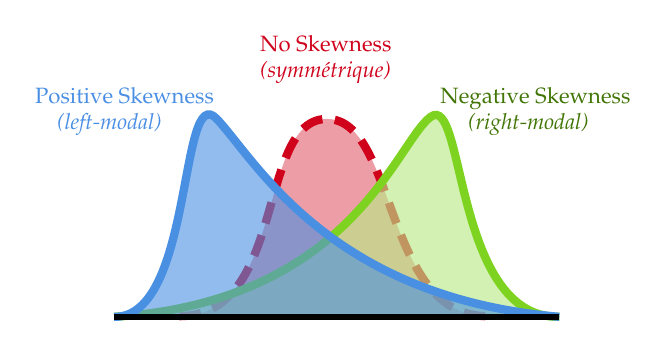
\begin{tikzpicture}[x=0.75pt,y=0.75pt,yscale=-1,xscale=1]
%uncomment if require: \path (0,300); %set diagram left start at 0, and has height of 300

%Curve Lines [id:da2688874623271533] 
\draw [color={rgb, 255:red, 208; green, 2; blue, 27 }  ,draw opacity=1 ][fill={rgb, 255:red, 208; green, 2; blue, 27 }  ,fill opacity=0.39 ][line width=3]  [dash pattern={on 7.88pt off 4.5pt}]  (80.5,138.67) .. controls (132.5,138.67) and (117.5,43.67) .. (151.5,43.67) .. controls (185.5,43.67) and (178.5,139.67) .. (229.5,138.67) ;


%Curve Lines [id:da9147539678395264] 
\draw [color={rgb, 255:red, 126; green, 211; blue, 33 }  ,draw opacity=1 ][fill={rgb, 255:red, 184; green, 233; blue, 134 }  ,fill opacity=0.64 ][line width=3]    (49,139) .. controls (163.5,131.67) and (184.83,55) .. (201.5,42.67) .. controls (218.17,30.33) and (212.5,140) .. (263.5,139) ;


%Curve Lines [id:da8124483083453555] 
\draw [color={rgb, 255:red, 74; green, 144; blue, 226 }  ,draw opacity=1 ][fill={rgb, 255:red, 74; green, 144; blue, 226 }  ,fill opacity=0.6 ][line width=3]    (49,139) .. controls (87.5,139.67) and (80.17,24.33) .. (98.5,43.67) .. controls (116.83,63) and (152.5,129.67) .. (263.5,139) ;

%Straight Lines [id:da7586443312018019] 
\draw [line width=2.25]    (49,139) -- (263.5,139) ;


% Text Node
\draw (151,15) node [scale=0.8,color={rgb, 255:red, 208; green, 2; blue, 27 }  ,opacity=1 ] [align=left] {No Skewness\\\textit{(symmétrique)}};
% Text Node
\draw (252,40) node [scale=0.8,color={rgb, 255:red, 65; green, 117; blue, 5 }  ,opacity=1 ] [align=left] {Negative Skewness\\\textit{ \ \ \ \ (right-modal)}};
% Text Node
\draw (54,40) node [scale=0.8,color={rgb, 255:red, 65; green, 117; blue, 5 }  ,opacity=1 ] [align=left] {\textcolor[rgb]{0.29,0.56,0.89}{Positive Skewness}\\\textit{\textcolor[rgb]{0.29,0.56,0.89}{ \ \ \ \ (left-modal)}}};
\end{tikzpicture}
\end{center}
\end{definitionNOHFILLsub}

\begin{definitionNOHFILLsub}[Kurtosis]
\lfbox[formula]{$\text{Kurtosis}	=	\frac{\mu_{4}}{\sigma^{4}}		=	\frac{\mu'_{4} - 4\mu'_{3}\mu + 6\mu'_{2}\mu^{2} - 3\mu^{4}}{\sigma^{3}}$}.\\

Le kurtosis mesure l'aplatissement d'une distribution et peut aider à juger la vraisemblance qu'une distribution produise des valeurs extrêmes (ou \og \textit{outliers} \fg{}).\\

Le kurtosis de la distribution normale est de 3. On pose qu'il est plus vraisemblable pour une distribution dont le kurtosis supérieur à 3 de produire des valeurs extrêmes.


\begin{center}
\tikzset{every picture/.style={line width=0.75pt}} %set default line width to 0.75pt        
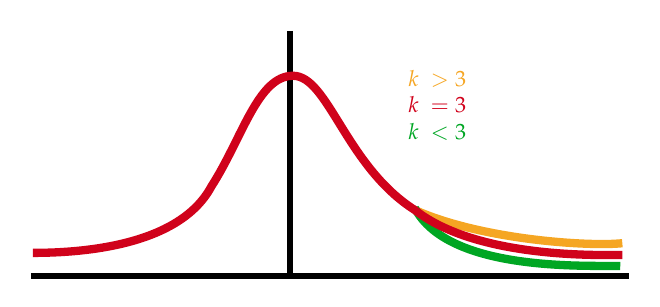
\begin{tikzpicture}[x=0.75pt,y=0.75pt,yscale=-1,xscale=1]
%Curve Lines [id:da18622021578279613] 
\draw [color={rgb, 255:red, 245; green, 166; blue, 35 }  ,draw opacity=1 ][line width=3]    (219.17,255.33) .. controls (252.17,270) and (304.17,273) .. (319.17,271.33) ;
%Curve Lines [id:da37988280307937217] 
\draw [color={rgb, 255:red, 0; green, 166; blue, 35 }  ,draw opacity=1 ][line width=3]    (219.17,254.33) .. controls (235.17,285) and (300.17,282) .. (318.17,282.33) ;
%Straight Lines [id:da5412137305076621] 
\draw [line width=2.25]    (159.17,169) -- (159.17,286) ;
%Curve Lines [id:da11948970250620294] 
\draw [color={rgb, 255:red, 208; green, 2; blue, 27 }  ,draw opacity=1 ][line width=3]    (35.17,276) .. controls (61.17,276) and (106.17,272) .. (121.17,244) .. controls (136.04,220.92) and (143.5,190.67) .. (160.5,190.67) .. controls (177.5,190.67) and (185.87,234.17) .. (219.17,255.33) .. controls (249.17,279) and (309.17,277) .. (319.17,277) ;
%Straight Lines [id:da09355877210927566] 
\draw [line width=2.25]    (34.17,287) -- (322.17,287) ;


% Text Node
\draw (230,206) node [scale=0.8,color={rgb, 255:red, 65; green, 117; blue, 5 }  ,opacity=1 ] [align=left] {$\displaystyle  \begin{array}{{>{\displaystyle}l}}
\textcolor[rgb]{0.96,0.65,0.14}{k\  >3}\\
\textcolor[rgb]{0.82,0.01,0.11}{k\ =3}\\
\textcolor[rgb]{0.0,0.65,0.14}{k\ < 3}
\end{array}$};
\end{tikzpicture}
\end{center}
\end{definitionNOHFILLsub}



\columnbreak
\subsection{Distributions}
\label{subsec:distrIARD}
\begin{definitionNOHFILLprop}[Loi Pareto]
\begin{rappel_enhanced}[Contexte]
La distribution Pareto est un mélange de deux distributions exponentielles originalement conçue pour étudier des distributions de revenus. 
\end{rappel_enhanced}

\begin{center}
\begin{tabular}{| >{\columncolor{beaublue}}c | >{\columncolor{beaublue}}c  | >{\columncolor{beaublue}}c  |}
\hline\rowcolor{airforceblue} 
\textcolor{white}{\textbf{Notation}}	&	\textcolor{white}{\textbf{Paramètres}}		&	\textcolor{white}{\textbf{Domaine}}	\\\specialrule{0.1em}{0em}{0em} 
$X \sim \text{Pareto}(\alpha, \theta)$	&	$\alpha, \theta	>	0$	&	$x \geq 0$	\\\hline
\end{tabular}
\end{center}

\begin{center}
\begin{tabular}{| >{\columncolor{airforceblue}}m{1cm} | >{\columncolor{beaublue}}m{4cm}  |}
\specialrule{0.1em}{0em}{0em}
\textcolor{white}{$f(x)$}	&	 \[=	\frac{\alpha\theta^{\alpha}}{(x + \theta)^{\alpha + 1}}\]		\\\specialrule{0.1em}{0em}{0em}
\textcolor{white}{$F(x)$}	&	 \[=1 -	\left(\frac{\theta}{x + \theta}\right)^{\alpha}\]		\\\specialrule{0.1em}{0em}{0em}
\end{tabular}
\end{center}

\begin{itemize}
	\item	Si $X \sim \text{Pareto}(\alpha, \theta)$ alors \lfbox[formula]{$Y	=	(X	-	d	|	X	>	d)	\sim \text{Pareto}(\alpha, \theta + d)$}.
\end{itemize}
\end{definitionNOHFILLprop}

\begin{definitionNOHFILLprop}[Loi Beta]
\begin{center}
\begin{tabular}{| >{\columncolor{beaublue}}c | >{\columncolor{beaublue}}c  | >{\columncolor{beaublue}}c  |}
\hline\rowcolor{airforceblue} 
\textcolor{white}{\textbf{Notation}}	&	\textcolor{white}{\textbf{Paramètres}}		&	\textcolor{white}{\textbf{Domaine}}	\\\specialrule{0.1em}{0em}{0em} 
$X \sim \text{Beta}(a, b, \theta)$	&	$a, b	>	0 \text{ et } \theta \geq 0$	&	$x \in [0, \theta]$	\\\hline
\end{tabular}
\end{center}

\begin{center}
\begin{tabular}{| >{\columncolor{airforceblue}}m{1cm} | >{\columncolor{beaublue}}m{4cm}  |}
\specialrule{0.1em}{0em}{0em}
\textcolor{white}{$f(x)$}	&	 \[= \frac{\theta}{\text{B}(a, b)}	\bigg(\frac{x}{\theta}\bigg)^{a - 1} \bigg(1 - \frac{x}{\theta}\bigg)^{b - 1}\]		\\\specialrule{0.1em}{0em}{0em}
\end{tabular}
\end{center}

\begin{itemize}
	\item	$X	\sim \text{Beta}(a = 1, b = 1, \theta) \sim \text{Unif}(0, \theta)$.
	\item	Si $X \sim \text{Unif}(a, b)$ alors  \lfbox[formula]{$(X	|	X	>	d)	\sim \text{Unif}(d, b)$} et \lfbox[formula]{$(X	-	d	|	X	>	d)	\sim \text{Unif}(0, b - d)$}.
\end{itemize}
\end{definitionNOHFILLprop}

\begin{definitionNOHFILLprop}[Loi Gamma]
\begin{center}
\begin{tabular}{| >{\columncolor{beaublue}}c | >{\columncolor{beaublue}}c  | >{\columncolor{beaublue}}c  |}
\hline\rowcolor{airforceblue} 
\textcolor{white}{\textbf{Notation}}	&	\textcolor{white}{\textbf{Paramètres}}		&	\textcolor{white}{\textbf{Domaine}}	\\\specialrule{0.1em}{0em}{0em} 
$X \sim \text{Gamma}(\alpha, \theta)$	&	$\alpha, \theta > 0$	&	$x \geq	0$	\\\hline
\end{tabular}
\end{center}

\begin{center}
\begin{tabular}{| >{\columncolor{airforceblue}}m{1cm} | >{\columncolor{beaublue}}m{4cm}  |}
\specialrule{0.1em}{0em}{0em}
\textcolor{white}{$f(x)$}	&	 \[= \frac{x^{\alpha - 1} \textrm{e}^{-x/\theta}}{\Gamma(\alpha)\theta^{\alpha}}\]		\\\specialrule{0.1em}{0em}{0em}
\end{tabular}
\end{center}

\begin{itemize}
	\item	On appelle $\theta$ la moyenne et $\lambda	=	\frac{1}{\theta}$ le paramètre de fréquence (\og \textit{rate} \fg{}).
	\item	Soit n v.a. indépendantes \lfbox[conditions]{$X_{i}	\sim \text{Gamma}(\alpha_{i}, \theta)$} alors \lfbox[formula]{$\sum_{i = 1}^{n} X_{i} \sim \text{Gamma}(\sum_{i = 1}^{n} \alpha_{i}, \theta)$}.
	\item	Soit n v.a. indépendantes \lfbox[conditions]{$X_{i}	\sim \text{Exp}(\lambda_{i})$} alors \lfbox[formula]{$Y	=	\min(X_{1}, \dots, X_{n})	\sim	\text{Exp}(\frac{1}{\sum_{i = 1}^{n} \lambda_{i})}$}.
	\item	Si $X \sim \text{Exp}(\theta)$ alors \lfbox[formula]{$(X	-	d	|	X	>	d)	\sim \text{Exp}(\theta)$}.
\end{itemize}
\end{definitionNOHFILLprop}


\begin{definitionNOHFILLprop}[Loi de Weibull]
\begin{center}
\begin{tabular}{| >{\columncolor{beaublue}}c | >{\columncolor{beaublue}}c  | >{\columncolor{beaublue}}c  |}
\hline\rowcolor{airforceblue} 
\textcolor{white}{\textbf{Notation}}	&	\textcolor{white}{\textbf{Paramètres}}		&	\textcolor{white}{\textbf{Domaine}}	\\\specialrule{0.1em}{0em}{0em} 
$X \sim \text{Weibull}(\tau, \beta)$	&	$\tau, \beta > 0$	&	$x \geq	0$	\\\hline
\end{tabular}
\end{center}

\begin{center}
\begin{tabular}{| >{\columncolor{airforceblue}}m{1cm} | >{\columncolor{beaublue}}m{4cm}  |}
\specialrule{0.1em}{0em}{0em}
\textcolor{white}{$f(x)$}	&	 \[= \frac{\tau (x/\theta)^{\tau} \textrm{e}^{-(x/\theta)^{\tau}}}{x}\]		\\\specialrule{0.1em}{0em}{0em}
\end{tabular}
\end{center}

\begin{itemize}
	\item	La loi de Weibull est une transformation de la loi exponentielle; pour \lfbox[conditions]{$Y \sim \text{Exp}(\mu)$}, alors \lfbox[formula]{$X = Y^{1/tau} \sim \text{Weibull}(\theta = \mu^{1/\tau}, \tau)$}.
\end{itemize}
\end{definitionNOHFILLprop}

\paragraph{Note}	Voir la sous-section \textit{\underline{\nameref{subsec:reliabilityVaria}}} de la section sur la \textit{\underline{\nameref{sec:reliability}}} du chapitre \textit{\underline{\nameref{chapt:varia}}} pour l'interprétation de la fonction de hasard dans le contexte de la loi gamma, la loi exponentielle et la loi de Weibull.


\begin{definitionNOHFILLprop}[Loi Erlang]
\begin{rappel_enhanced}[Contexte]
La loi Erlang est un cas spécial de la loi Gamma avec un paramètre de forme $\alpha$ entier. Elle est utile dans le contexte de \textbf{\nameref{sec:procPois}}, car nous pouvons trouver une forme explicite de la fonction de répartition (survie).
\end{rappel_enhanced}

\begin{center}
\begin{tabular}{| >{\columncolor{beaublue}}c | >{\columncolor{beaublue}}c  | >{\columncolor{beaublue}}c  |}
\hline\rowcolor{airforceblue} 
\textcolor{white}{\textbf{Notation}}	&	\textcolor{white}{\textbf{Paramètres}}		&	\textcolor{white}{\textbf{Domaine}}	\\\specialrule{0.1em}{0em}{0em} 
$X \sim \text{Erlang}(n, \lambda)$	&	$\lambda > 0$ et $n \in \mathbb{N}^{+}$	&	$x \geq	0$	\\\hline
\end{tabular}
\end{center}

\begin{center}
\begin{tabular}{| >{\columncolor{airforceblue}}m{1cm} | >{\columncolor{beaublue}}m{4cm}  |}
\specialrule{0.1em}{0em}{0em}
\textcolor{white}{$f(x)$}	&	 \[= \frac{x^{n - 1} \lambda^{n} \textrm{e}^{-\lambda x}}{\Gamma(n)}\]		\\\specialrule{0.1em}{0em}{0em}
\textcolor{white}{$S(x)$}	&	 \[= \sum_{k = 0}^{n - 1}\frac{(\lambda x)^{k - 1} \textrm{e}^{-\lambda x}}{k!}\]		\\\specialrule{0.1em}{0em}{0em}
\end{tabular}
\end{center}
\end{definitionNOHFILLprop}

\begin{definitionNOHFILLprop}[Loi de Poisson]
\begin{center}
\begin{tabular}{| >{\columncolor{beaublue}}c | >{\columncolor{beaublue}}c  | >{\columncolor{beaublue}}c  |}
\hline\rowcolor{airforceblue} 
\textcolor{white}{\textbf{Notation}}	&	\textcolor{white}{\textbf{Paramètres}}		&	\textcolor{white}{\textbf{Domaine}}	\\\specialrule{0.1em}{0em}{0em} 
$X \sim \text{Poisson}(\lambda)$	&	$\lambda	>	0$	&	$x = 0, 1, 2, \dots$	\\\hline
\end{tabular}
\end{center}

\begin{center}
\begin{tabular}{| >{\columncolor{airforceblue}}m{2cm} | >{\columncolor{beaublue}}m{4cm}  |}
\specialrule{0.1em}{0em}{0em}
\textcolor{white}{$\Pr(X = x)$}	&	 \[=\frac{\textrm{e}^{-\lambda} \lambda^{x}}{x!}\]		\\\specialrule{0.1em}{0em}{0em}
\end{tabular}
\end{center}
\end{definitionNOHFILLprop}


\columnbreak
\subsection{Transformation}
\begin{definitionNOHFILLsub}[Changement d'échelle pour des v.a. continues]
Toutes les distributions continues (sauf pour la lognormale, l'inverse gaussienne et la log-t) ont $\theta$ comme paramètre d'échelle. Alors, multiplier la v.a. par une constante $c$ change uniquement le paramètre $\theta^{\ast}	=	c\theta$.
\end{definitionNOHFILLsub}

\begin{algo2}[Trouver la PDF d'une v.a. transformée]
Soit $n$ v.a. $X_{1}, \dots, X_{n}$ que l'on veut transformer en $n$ autres variables aléatoires $W_{1}	=	g_{1}(X_{1}, \dots, X_{n}), \dots, W_{n}	=	g_{n}(X_{1}, \dots, X_{n})$.
\begin{enumerate}[label	=	\circled{\arabic*}{trueblue}]
	\item	Trouver les inverses des équations de la transformation : 
		\begin{align*}
		x_{1}	
		&=	g^{-1}_{1}(w_{1}, \dots, w_{n})	\\
		\vdots	\\
		x_{n}	
		&=	g^{-1}_{n}(w_{1}, \dots, w_{n})	
		\end{align*}
	\item	Calculer le déterminant de la matrice Jacobienne $J$ : 
		\begin{align*}
		J
		&=	\det \begin{bmatrix}
		\deriv{w_{1}}{x_{1}}	&	\hdots	&	\deriv{w_{n}}{x_{1}}	\\
		\vdots	&	\ddots	&	\vdots	\\
		\deriv{w_{1}}{x_{n}}		&	\hdots	&	\deriv{w_{n}}{x_{n}}
		\end{bmatrix}
		\end{align*}
	\item	Trouver la fonction de densité conjointe avec 
\end{enumerate}
\lfbox[formula]{$f_{W_{1}, \dots, W_{n}}(w_{1}, \dots, w_{n})	=	f_{X_{1}, \dots, X_{n}}\left(g^{-1}_{1}(w_{1}, \dots, w_{n}), \dots, g^{-1}_{n}(w_{1}, \dots, w_{n})\right) |J|$}.

\paragraph{Note}	Dans le cas univarié, \lfbox[formula]{$f_{W}(w)	=	f_{X}\left(g^{-1}(w)\right) \left|\deriv{w}{g^{-1}(w)}\right|$}.
\end{algo2}


\columnbreak
\subsection{Queues de distributions}
\begin{rappel_enhanced}[Contexte]
Si une distribution a une queue de droite qui est lourde, \og \textit{thick} \fg{} ou \og \textit{fat} \fg{}, alors elle a des probabilités élevées de pertes extrêmes.
\end{rappel_enhanced}

En situation d'examen nous ne pouvons pas visuellement évaluer la queue et donc nous utilisons un des 4 tests suivants :
\begin{definitionGENERAL}{Nombre de moments (positifs) qui existent}[\circled{1}{trueblue}]
\textit{Plus} la queue est \textbf{\textbf{\textcolor{teal}{lourde}}}, \textit{\textcolor{teal}{moins}} il y a de moments qui existent.\\

\begin{itemize}
	\item	Il devient de moins en moins probable que l'intégrale de $x^{k}f(x)$ va converger.
\end{itemize}
\end{definitionGENERAL}

\begin{definitionGENERAL}{Ratio des fonctions de survie (ou PDF)}[\circled{2}{trueblue}]
\textit{Plus} la queue est \textbf{\textbf{\textcolor{teal}{lourde}}}, \textit{\textcolor{teal}{plus}} la fonction de \textcolor{teal}{survie va tendre vers 0 \textit{\textbf{lentement}}}.\\

\begin{itemize}
	\item	Si $\limz{x}{\infty} \frac{S_{1}(x)}{S_{2}(x)}	=	0$ alors $X_{1}$ a une queue plus légère que $X_{2}$, et vice-versa si la limite tend vers $\infty$.
	\item	Par la règle de l'hôpital, ceci est équivalent pour le ratio des PDF.
\end{itemize}
\end{definitionGENERAL}

\begin{definitionGENERAL}{Fonctions de hasard}[\circled{3}{trueblue}]
Si la \textcolor{teal}{fonction de hasard} est \textit{\textcolor{teal}{décroissante}}, il y a une probabilité plus élevée de pertes extrêmes et donc une queue \textit{\textbf{\textcolor{teal}{lourde}}}.
\end{definitionGENERAL}

\begin{definitionGENERAL}{CTEs (ou quantiles)}[\circled{4}{trueblue}]
\textbf{\textit{\textcolor{teal}{Plus}}} le \textcolor{teal}{CTE (ou les quantiles) est large}, plus les montants de pertes extrêmes sont larges et donc \textit{plus} la queue est \textit{\textbf{\textcolor{teal}{lourde}}}.
\end{definitionGENERAL}



\pagebreak
\section{Estimations et types de données}
\subsection{Distributions empiriques}
\begin{distributions}[Notation]
\begin{description}
	\item[$X$]	Variable aléatoire de perte;
	\item[$\theta$]	Paramètre de la distribution de $X$;
		\begin{itemize}[leftmargin = *]
		\item	Le paramètre peut être un scalaire $\theta$ ou un vecteur $\bm{\theta}$;
		\item	Par exemple, pour une loi Gamma $\bm{\theta} = \{\alpha,	\beta\}$;
		\item	Pour simplifier la notation, on le traite comme un scalaire $\theta$.
		\end{itemize}
	\item[$F_{X}(x; \theta)$]	Fonction de répartition de $X$ avec paramètre $\theta$;
		\begin{itemize}[leftmargin = *]
		\item	Pour simplifier la notation, on écrit $F(x; \theta)$ sauf s'il faut être plus spécifique.
		\end{itemize}
	\item[$f_{X}(x; \theta)$]	Fonction de densité de $X$ avec paramètre $\theta$;
		\begin{itemize}[leftmargin = *]
		\item	Pour simplifier la notation, on écrit $f(x; \theta)$ sauf s'il faut être plus spécifique.
		\end{itemize}
	\item[$\{X_{1}, \dots, X_{n}\}$]	Échantillon aléatoire de $n$ observations de $X$;
	\item[$\hat{\theta}$]	Estimateur de $\theta$ établit avec l'échantillon aléatoire $\{X_{1}, \dots, X_{n}\}$;
	\item[$F(x; \hat{\theta})$]	Estimation \textit{paramétrique} de la fonction de répartition de $X$;
	\item[$f(x; \hat{\theta})$]	Estimation \textit{paramétrique} de la fonction de densité de $X$;
\end{description}
\end{distributions}
\begin{itemize}[leftmargin = *]
	\item	Si $\theta$ est connu, la distribution de $X$ est complètement spécifiée;\\
			En pratique, $\theta$ est inconnu et doit être estimé avec les données observées.
	\item	On peut estimer $F_{X}(x)$ et $f_{X}(x)$ directement pour toute valeur $x$ sans présumer une forme paramétrique;\\
			Par exemple, un histogramme est une estimation \textit{non paramétrique}.
\end{itemize}


\columnbreak
\subsection{Données complètes}
\begin{distributions}[Notation]
\begin{description}
	\item[$X$]	Variable d'intérêt (p. ex., la durée de vie ou la perte);
	\item[$\{X_{1}, \dots, X_{n}\}$]	Valeurs de $X$ pour n individus;
	\item[$\{x_{1}, \dots, x_{n}\}$]	$n$ valeurs observées de l'échantillon;
		\begin{itemize}[leftmargin = *]
		\item	Il peut y avoir des valeurs dupliquées dans les valeurs observées.
		\end{itemize}
	\item[$0	<	y_{1}	<	\hdots	<	y_{m}$]	$m$ valeurs distinctes où \icbox[red][palechestnut]{$m \leq n$};
	\item[$w_{j}$]	Nombre de fois que la valeur $y_{j}$ apparaît dans l'échantillon pour \icbox[red][palechestnut]{$j = 1, \dots, m$};
		\begin{itemize}[leftmargin = *]
		\item	Il s'ensuit que \icbox[red][palechestnut]{$\sumz{m}{j = 1}w_{j}	=	n$};
		\item	Pour des données de mortalité, $w_{j}$ individus décèdent à l'âge $y_{j}$;
		\item	Si tous les individus sont observés de la naissance jusqu'à la mort c'est un \og \textit{complete individual data set} \fg{}.
		\end{itemize}
	\item[$r_{j}$]	\og \textit{risk set} \fg{} au \textit{temps} $y_{j}$;
		\begin{itemize}[leftmargin = *]
		\item	Le nombre d'individus exposés à la possibilité de mourir au temps $y_{j}$;
		\item	Par exemple, $r_{1}	=	n$, car tous les individus sont exposés au risque de décéder juste avant le temps $y_{1}$;
		\item	On déduit que \icbox[red][palechestnut]{$r_{j}	=	\sumz{m}{i = j}w_{i}$}, alias le nombre d'individus qui survivent juste avant le temps $y_{j}$.
		\end{itemize}
\end{description}
\end{distributions}

\columnbreak
\subsection{Données incomplètes}

\begin{rappel_enhanced}[Exemple]
Soit une étude sur le nombre d'années nécessaire pour obtenir un diplôme universitaire. L'étude commence cette année et tient compte de tous les étudiants présentement inscrits, ainsi que ceux qui vont s'inscrire au courant de l'étude. Tous les étudiants sont observés jusqu'à la fin de l'étude et on note le nombre d'années nécessaire pour ceux qui complètent leurs diplômes. \\

Si un étudiant a commencé son cursus scolaire avant l'étude et suit présentement des cours, le chercheur a de l'information sur le nombre d'années qu'il a déjà investi. Cependant, d'autres étudiants qui se sont inscrits en même temps, mais ont cessé leurs études ne seront pas observés dans cet échantillon. Alors, l'individu est observé d'une population \lfbox[imphl]{\textbf{tronquée à la gauche}} puisque l'information sur les étudiants qui ont quitté l'université avant le début de l'étude n'est \textit{pas disponible}.\\

Si un étudiant n'est pas encore diplômé lorsque l'étude prend fin, le chercheur ne peut pas savoir combien d'années supplémentaires seront nécessaires. Cet individu fait donc partie d'une population \lfbox[imphl]{\textbf{censurée à la droite}} puisque le chercheur a de l'information \textit{partielle} (le nombre d'années minimal) sans savoir le nombre exact.
\end{rappel_enhanced}

\begin{distributions}[Notation]
\begin{description}
	\item[$d_{i}$]	État de troncature de l'individu $i$ de l'échantillon;
		\begin{itemize}[leftmargin = *]
		\item	$d_{i}	=	0$ s'il n'y a pas de troncature;
		\item	Par exemple, un étudiant a commencé son programme universitaire $d_{i}$ années avant le début de l'étude.
		\end{itemize}
	\item[$x_{i}$]	Temps de "survie" de l'individu $i$;
		\begin{itemize}[leftmargin = *]
		\item	Par exemple, le nombre d'années avant d'obtenir son diplôme;
		\item	Si l'étude prend fin avant que $x_{i}$ soit observé, on dénote le temps de survie jusqu'à ce moment \icbox{$u_{i}$};
		\item	Donc chaque individu a \textit{soit} une valeur $x_{i}$ \underline{ou} $u_{i}$, mais \textit{pas les deux}.
		\end{itemize}
\end{description}
\end{distributions}

\columnbreak
\subsection{Données groupées}
\begin{distributions}[Notation]
\begin{description}
	\item[]	$(c_{0}, c_{1}], (c_{1}, c_{2}], \dots, (c_{k - 1}, c_{k}]$	$k$ intervalles regroupant les observations;
	\item[$0	\leq	c_{0}	<	c_{1}	<	\hdots	<	c_{k}$]	Extrémités des $k$ intervalles;
	\item[$n$]	Nombre d'observations de $x_{i}$ dans l'échantillon;
	\item[$n_{j}$]	Nombre d'observations de $x_{i}$ dans l'intervalle $(c_{j - 1}, c_{j}]$;
		\begin{itemize}[leftmargin = *]
		\item	Il s'ensuit que \icbox[red][palechestnut]{$\sumz{k}{j = 1}n_{j}	=	n$}.
		\end{itemize}
	\item[$r_{j}$]	\og \textit{risk set} \fg{} de l'intervalle $(c_{j - 1}, c_{j}]$ lorsque les données sont complètes;
		\begin{itemize}[leftmargin = *]
		\item	Il s'ensuit que \icbox[red][palechestnut]{$r_{j}	=	\sumz{k}{i = j}n_{i}$}.
		\end{itemize}
\end{description}
\end{distributions}


\columnbreak
\section{Applications en assurance}
\begin{distributions}[Notation]
\begin{description}
	\item[$X$]	Variable aléatoire du montant de perte.
\end{description}
\end{distributions}


\subsection{Limite de police}
\begin{definitionNOHFILL}[Limite de police]
Une \textbf{limite de police} \lfbox[formula]{$u$} est le montant maximal qu'un assureur va payer pour une perte.\\


Visuellement : 
\begin{center}


\tikzset{every picture/.style={line width=0.75pt}} %set default line width to 0.75pt        

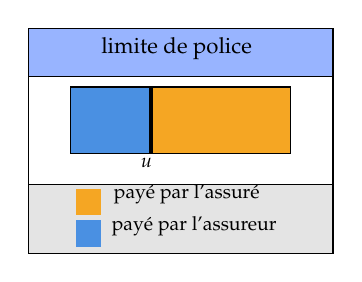
\begin{tikzpicture}[x=0.75pt,y=0.75pt,yscale=-1,xscale=1]
%uncomment if require: \path (0,154); %set diagram left start at 0, and has height of 154

%Shape: Rectangle [id:dp02803686274972339] 
\draw  [fill={rgb, 255:red, 255; green, 255; blue, 255 }  ,fill opacity=1 ] (311,17.67) -- (457.83,17.67) -- (457.83,126) -- (311,126) -- cycle ;
%Shape: Rectangle [id:dp6650428705496374] 
\draw  [fill={rgb, 255:red, 228; green, 228; blue, 228 }  ,fill opacity=1 ] (311,93) -- (457.83,93) -- (457.83,126) -- (311,126) -- cycle ;
%Shape: Rectangle [id:dp011257611005494716] 
\draw  [fill={rgb, 255:red, 152; green, 180; blue, 255 }  ,fill opacity=1 ] (311,17.67) -- (457.83,17.67) -- (457.83,41) -- (311,41) -- cycle ;
%Shape: Rectangle [id:dp9403819194026608] 
\draw  [draw opacity=0][fill={rgb, 255:red, 245; green, 166; blue, 35 }  ,fill opacity=1 ] (370,46) -- (437.5,46) -- (437.5,78) -- (370,78) -- cycle ;
%Shape: Rectangle [id:dp48392000225673093] 
\draw  [draw opacity=0][fill={rgb, 255:red, 74; green, 144; blue, 226 }  ,fill opacity=1 ] (331.33,46) -- (370,46) -- (370,78) -- (331.33,78) -- cycle ;
%Shape: Rectangle [id:dp7277326812364118] 
\draw   (331.33,46) -- (437.5,46) -- (437.5,78) -- (331.33,78) -- cycle ;
%Straight Lines [id:da8740810297553647] 
\draw [line width=1.5]    (370,46) -- (370,78) ;
%Shape: Rectangle [id:dp4533678374731276] 
\draw  [draw opacity=0][fill={rgb, 255:red, 245; green, 166; blue, 35 }  ,fill opacity=1 ] (333.83,94.97) -- (346.17,94.97) -- (346.17,107.7) -- (333.83,107.7) -- cycle ;
%Shape: Rectangle [id:dp2562930482964858] 
\draw  [draw opacity=0][fill={rgb, 255:red, 74; green, 144; blue, 226 }  ,fill opacity=1 ] (333.83,110.13) -- (346.17,110.13) -- (346.17,122.87) -- (333.83,122.87) -- cycle ;

% Text Node
\draw (344.92,20.67) node [anchor=north west][inner sep=0.75pt]   [align=left] {{\footnotesize limite de police}};
% Text Node
\draw (351,91.83) node [anchor=north west][inner sep=0.75pt]   [align=left] {{\scriptsize payé par l'assuré}};
% Text Node
\draw (350,107) node [anchor=north west][inner sep=0.75pt]   [align=left] {{\scriptsize payé par l'assureur}};
% Text Node
\draw (364,79) node [anchor=north west][inner sep=0.75pt]  [font=\scriptsize] [align=left] {$\displaystyle u$};


\end{tikzpicture}
\end{center}
\end{definitionNOHFILL}

\begin{definitionNOHFILLsub}[Montant de perte limité]
La variable aléatoire du \textbf{montant de perte limité} \lfbox[formula]{$X \wedge u$} correspond au montant du paiement de l'assureur pour une police d'assurance ayant une limite de $u$ :

\begin{align*}
	X \wedge u
	&=	\begin{cases}
		X,	&	X < u	\\
		u,	&	X \geq u	\\
		\end{cases}
\end{align*}
\begin{itemize}
	\item	Il s'ensuit que \lfbox[formula]{$X \wedge d	=	\min(X; d)$}.
\end{itemize}

Visuellement : 

\begin{center}
\tikzset{every picture/.style={line width=0.75pt}} %set default line width to 0.75pt        
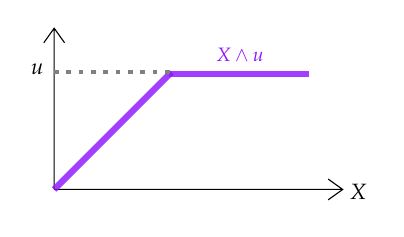
\begin{tikzpicture}[x=0.75pt,y=0.75pt,yscale=-1,xscale=1]
%uncomment if require: \path (0,174); %set diagram left start at 0, and has height of 174

%Shape: Axis 2D [id:dp6598259573253495] 
\draw  (313.5,139) -- (452.5,139)(313.5,61.33) -- (313.5,139) -- cycle (445.5,134) -- (452.5,139) -- (445.5,144) (308.5,68.33) -- (313.5,61.33) -- (318.5,68.33)  ;
%Straight Lines [id:da2579967683196891] 
\draw [color={rgb, 255:red, 142; green, 19; blue, 254 }  ,draw opacity=0.82 ][line width=2.25]    (313.5,139) -- (370,82.5) ;
%Straight Lines [id:da18638822683919853] 
\draw [color={rgb, 255:red, 142; green, 19; blue, 254 }  ,draw opacity=0.82 ][line width=2.25]    (369,83.5) -- (436.46,83.5) ;
%Straight Lines [id:da08876956095236466] 
\draw [color={rgb, 255:red, 128; green, 128; blue, 128 }  ,draw opacity=1 ][line width=1.5]  [dash pattern={on 1.69pt off 2.76pt}]  (313.5,82.5) -- (370,82.5) ;

% Text Node
\draw (460,140) node  [font=\footnotesize] [align=left] {$\displaystyle X$};
% Text Node
\draw (403,74) node  [font=\scriptsize,color={rgb, 255:red, 144; green, 19; blue, 254 }  ,opacity=1 ] [align=left] {$\displaystyle X\land u$};
% Text Node
\draw (301,77) node [anchor=north west][inner sep=0.75pt]  [font=\footnotesize] [align=left] {$\displaystyle u$};


\end{tikzpicture}
\end{center}
\end{definitionNOHFILLsub}

\begin{definitionNOHFILLsub}[L'espérance limitée du montant de perte]
\textbf{L'espérance limitée du montant de perte} \lfbox[formula]{$\text{E}[X \wedge u]$} correspond à l'espérance du paiement de l'assureur pour une police d'assurance ayant une limite de $u$ :

\begin{align*}
	\text{E}[X \wedge u]	
	&=	\int_{0}^{u} x f(x) dx + u S(u)
\end{align*}
\end{definitionNOHFILLsub}


\columnbreak
\subsection{Déductibles}
\begin{definitionNOHFILL}[Déductible]
Le \textbf{déductible d'une police} est le montant que l'assuré doit payer de sa poche avant que l'assureur débourse pour une perte. \\

Il y a 2 types de déductibles : 
\begin{description}
	\item[déductible ordinaire]	Une fois que le montant de perte surpasse le déductible, l'assureur va payer le montant de la perte \textbf{en excès du déductible}.
	\item[déductible de franchise]	Une fois que le montant de perte surpasse le déductible, l'assureur va payer le montant \textbf{total} de la perte.
\end{description}

Par défaut, on suppose le déductible ordinaire.\\

Visuellement :

\begin{center}
\tikzset{every picture/.style={line width=0.75pt}} %set default line width to 0.75pt        
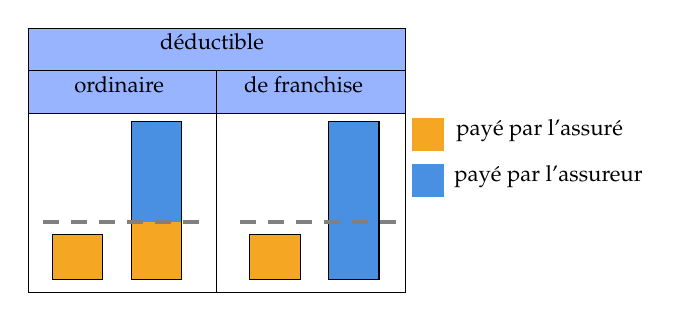
\begin{tikzpicture}[x=0.75pt,y=0.75pt,yscale=-1,xscale=1]
%uncomment if require: \path (0,217); %set diagram left start at 0, and has height of 217

%Shape: Rectangle [id:dp588617566986505] 
\draw  [draw opacity=0][fill={rgb, 255:red, 245; green, 166; blue, 35 }  ,fill opacity=1 ] (128.75,134.92) -- (128.75,113.33) -- (152.99,113.33) -- (152.99,134.92) -- cycle ;
%Shape: Rectangle [id:dp003856682054647287] 
\draw   (128.75,134.92) -- (128.75,113.33) -- (152.99,113.33) -- (152.99,134.92) -- cycle ;
%Shape: Rectangle [id:dp700556830555261] 
\draw  [draw opacity=0][fill={rgb, 255:red, 245; green, 166; blue, 35 }  ,fill opacity=1 ] (301.83,56.92) -- (317.17,56.92) -- (317.17,72.75) -- (301.83,72.75) -- cycle ;
%Shape: Rectangle [id:dp7089085688842631] 
\draw  [draw opacity=0][fill={rgb, 255:red, 74; green, 144; blue, 226 }  ,fill opacity=1 ] (301.83,79) -- (317.33,79) -- (317.33,95) -- (301.83,95) -- cycle ;
%Shape: Rectangle [id:dp40057299526008183] 
\draw  [draw opacity=0][fill={rgb, 255:red, 74; green, 144; blue, 226 }  ,fill opacity=1 ] (166.75,107.14) -- (166.75,58.67) -- (190.99,58.67) -- (190.99,107.14) -- cycle ;
%Shape: Rectangle [id:dp7752631736808828] 
\draw  [draw opacity=0][fill={rgb, 255:red, 245; green, 166; blue, 35 }  ,fill opacity=1 ] (166.75,134.92) -- (166.75,107.14) -- (190.99,107.14) -- (190.99,134.92) -- cycle ;
%Shape: Rectangle [id:dp8322518421090499] 
\draw   (166.75,134.92) -- (166.75,58.67) -- (190.99,58.67) -- (190.99,134.92) -- cycle ;
%Straight Lines [id:da21204533122634284] 
\draw [color={rgb, 255:red, 128; green, 128; blue, 128 }  ,draw opacity=1 ][line width=1.5]  [dash pattern={on 5.63pt off 4.5pt}]  (124.17,107) -- (200.17,107) ;
%Shape: Rectangle [id:dp10210761313509842] 
\draw  [draw opacity=0][fill={rgb, 255:red, 245; green, 166; blue, 35 }  ,fill opacity=1 ] (223.75,134.92) -- (223.75,113.33) -- (247.99,113.33) -- (247.99,134.92) -- cycle ;
%Shape: Rectangle [id:dp1422285500093443] 
\draw   (223.75,134.92) -- (223.75,113.33) -- (247.99,113.33) -- (247.99,134.92) -- cycle ;
%Shape: Rectangle [id:dp3614273531351382] 
\draw  [draw opacity=0][fill={rgb, 255:red, 74; green, 144; blue, 226 }  ,fill opacity=1 ] (261.75,134.92) -- (261.75,58.67) -- (285.99,58.67) -- (285.99,134.92) -- cycle ;
%Shape: Rectangle [id:dp4016556775232154] 
\draw   (261.75,134.92) -- (261.75,58.67) -- (285.99,58.67) -- (285.99,134.92) -- cycle ;
%Straight Lines [id:da9540437083363307] 
\draw [color={rgb, 255:red, 128; green, 128; blue, 128 }  ,draw opacity=1 ][line width=1.5]  [dash pattern={on 5.63pt off 4.5pt}]  (219.17,107) -- (295.17,107) ;
%Shape: Rectangle [id:dp7792912132142298] 
\draw   (117,43) -- (207.83,43) -- (207.83,141.33) -- (117,141.33) -- cycle ;
%Shape: Rectangle [id:dp19600907651515787] 
\draw  [fill={rgb, 255:red, 152; green, 180; blue, 255 }  ,fill opacity=1 ] (117,34.33) -- (207.83,34.33) -- (207.83,54.85) -- (117,54.85) -- cycle ;
%Shape: Rectangle [id:dp25767783018946355] 
\draw   (207.83,43) -- (298.67,43) -- (298.67,141.33) -- (207.83,141.33) -- cycle ;
%Shape: Rectangle [id:dp6656766828727914] 
\draw  [fill={rgb, 255:red, 152; green, 180; blue, 255 }  ,fill opacity=1 ] (207.83,34.33) -- (298.67,34.33) -- (298.67,54.85) -- (207.83,54.85) -- cycle ;
%Shape: Rectangle [id:dp932544307028238] 
\draw  [fill={rgb, 255:red, 152; green, 180; blue, 255 }  ,fill opacity=1 ] (117,13.82) -- (298.67,13.82) -- (298.67,34.33) -- (117,34.33) -- cycle ;

% Text Node
\draw (137.92,35.76) node [anchor=north west][inner sep=0.75pt]   [align=left] {{\footnotesize ordinaire}};
% Text Node
\draw (322,56.33) node [anchor=north west][inner sep=0.75pt]   [align=left] {{\footnotesize payé par l'assuré}};
% Text Node
\draw (321,78.5) node [anchor=north west][inner sep=0.75pt]   [align=left] {{\footnotesize payé par l'assureur}};
% Text Node
\draw (219.75,35.76) node [anchor=north west][inner sep=0.75pt]   [align=left] {{\footnotesize de franchise}};
% Text Node
\draw (179.33,15.05) node [anchor=north west][inner sep=0.75pt]   [align=left] {{\footnotesize déductible}};


\end{tikzpicture}
\end{center}
\end{definitionNOHFILL}


\subsubsection{Déductible ordinaire}
\begin{definitionNOHFILLsub}[Montant de perte avec un déductible \textbf{ordinaire}]
La variable aléatoire du montant de perte pour une police ayant un \textbf{déductible ordinaire} de $d$. \\

\begin{minipage}[ht]{0.5\columnwidth}
\begin{center}
	Assureur
\end{center}
\begin{align*}
	(X - d)_{+}
	&=	\begin{cases}
		0,	  	&	X \leq d	\\
		X - d,	&	X > d	
		\end{cases}
\end{align*}
\end{minipage}%
\begin{minipage}[ht]{0.5\columnwidth}
\begin{center}
	Assuré
\end{center}
\begin{align*}
	X \wedge d
	&=	\begin{cases}
		X,  &	X < d	\\
		d,	&	X \geq d	
		\end{cases}
\end{align*}
\end{minipage}

\

\begin{itemize}
	\item	Il s'ensuit que \lfbox[formula]{$(X - d)_{+}	=	\max(X - d; 0)$}.
	\item	On observe que le montant de perte est la somme des contributions \lfbox[conditions]{$X	=	X \wedge d + (X - d)_{+}$}.
\end{itemize}

Visuellement :
\begin{center}
\tikzset{every picture/.style={line width=0.75pt}} %set default line width to 0.75pt        
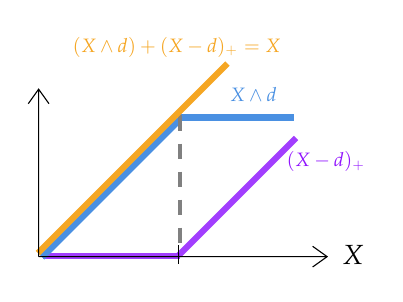
\begin{tikzpicture}[x=0.75pt,y=0.75pt,yscale=-1,xscale=1]
%uncomment if require: \path (0,155); %set diagram left start at 0, and has height of 155

%Straight Lines [id:da2658768489155079] 
\draw [color={rgb, 255:red, 142; green, 19; blue, 254 }  ,draw opacity=0.82 ][line width=2.25]    (429,118.33) -- (485.5,61.83) ;
%Straight Lines [id:da11698723071359618] 
\draw [color={rgb, 255:red, 142; green, 19; blue, 254 }  ,draw opacity=0.82 ][line width=2.25]    (363.54,118.62) -- (429.67,118.62) ;
%Straight Lines [id:da326418494508391] 
\draw [color={rgb, 255:red, 74; green, 144; blue, 226 }  ,draw opacity=1 ][line width=2.25]    (363.17,119.33) -- (429.5,53) ;
%Straight Lines [id:da8149304204229495] 
\draw [color={rgb, 255:red, 74; green, 144; blue, 226 }  ,draw opacity=1 ][line width=2.25]    (429.5,52) -- (484.5,52) ;
%Straight Lines [id:da6292319909047852] 
\draw [color={rgb, 255:red, 128; green, 128; blue, 128 }  ,draw opacity=1 ][line width=1.5]  [dash pattern={on 5.63pt off 4.5pt}]  (429.5,51) -- (429.5,117.62) ;
%Straight Lines [id:da12597396522940518] 
\draw    (429,122.33) -- (429,113.33) ;
%Straight Lines [id:da048934088668804776] 
\draw [color={rgb, 255:red, 245; green, 166; blue, 35 }  ,draw opacity=1 ][line width=2.25]    (361.17,117.33) -- (452.5,26) ;
%Shape: Axis 2D [id:dp3636642155394634] 
\draw  (361.5,119) -- (500.5,119)(361.5,38.33) -- (361.5,119) -- cycle (493.5,114) -- (500.5,119) -- (493.5,124) (356.5,45.33) -- (361.5,38.33) -- (366.5,45.33)  ;

% Text Node
\draw (513,118) node   [align=left] {$\displaystyle X$};
% Text Node
\draw (500,73) node  [font=\scriptsize,color={rgb, 255:red, 144; green, 19; blue, 254 }  ,opacity=1 ] [align=left] {$\displaystyle ( X-d)_{+}$};
% Text Node
\draw (465,41) node  [font=\scriptsize,color={rgb, 255:red, 74; green, 144; blue, 226 }  ,opacity=1 ] [align=left] {$\displaystyle X\land d$};
% Text Node
\draw (428,18) node  [font=\scriptsize,color={rgb, 255:red, 245; green, 166; blue, 35 }  ,opacity=1 ] [align=left] {$\displaystyle ( X\land d) +( X-d)_{+} =X$};


\end{tikzpicture}
\end{center}
\end{definitionNOHFILLsub}

\begin{definitionNOHFILLsub}[L'espérance du montant de perte avec un déductible ordinaire]
\textbf{L'espérance du montant de perte}, pour l'assureur, \textbf{avec un déductible \textit{ordinaire}} \lfbox[formula]{$\text{E}[(X - d)_{+}]$} correspond à :

\begin{align*}
	\text{E}[(X - d)_{+}]
	&=	\int_{d}^{\infty} (x - d) f(x) dx
\end{align*}
\end{definitionNOHFILLsub}

\begin{definitionNOHFILLprop}[\og \textit{Loss Elimination Ratio (LER)} \fg{}]
Le \og \textit{Loss Elimination Ratio (LER)} \fg{} évalue combien qu'épargne l'assureur en imposant un déductible \textit{ordinaire} de $d$,
\lfbox[formula]{$LER	=	\frac{\text{E}[X \wedge d]}{\text{E}[X]}$}.
\end{definitionNOHFILLprop}


\subsubsection{\og \textit{payment \textbf{per loss}} \fg{} et \og \textit{payment \textbf{per payment}} \fg{}}
\begin{distributions}[Notation]
\begin{description}
	\item[$Y^{L}$]	Montant de perte.
		\begin{itemize}
		\item	\og \textit{payment per \textbf{l}oss} \fg{}
		\end{itemize}
	\item[$Y^{P}$]	Montant de paiement.
		\begin{itemize}
		\item	\og \textit{payment per \textbf{p}ayment} \fg{}
		\end{itemize}
\end{description}
\end{distributions}

\begin{description}
	\item[$\text{E}\lbrack Y^{L} \rbrack$]	Montant espéré de paiement \textbf{par perte \textit{subie}}.
	\item[$\text{E}\lbrack Y^{P}\rbrack$]	Montant espéré de paiement \textbf{par paiement \textit{effectué}}.
		\begin{itemize}
		\item	Par exemple, lorsqu'une police a un déductible, les pertes dont le coût est inférieur au déductible ne seront pas reportées à l'assureur.
		\item	Le montant de paiement est donc le montant que l'assureur va payer conditionnel à ce qu'il y ait un paiement.
		\item	Il s'ensuit que \lfbox[conditions]{$\text{E}[Y^{L}] \geq \text{E}[Y^{L}]$}.
		\end{itemize}
\end{description}


Pour un déductible ordinaire de $d$, 

\begin{minipage}[ht]{0.5\columnwidth}
\begin{align*}
	\text{E}[Y^{L}]
	&=	\text{E}[(X - d)_{+}]
\end{align*}
\end{minipage}%
\begin{minipage}[ht]{0.5\columnwidth}
\begin{align*}
	\text{E}[Y^{P}]
	&=	\text{E}[X - d | X > d]
\end{align*}
\end{minipage}

\begin{itemize}
	\item	On trouve que \lfbox[formula]{$\text{E}[Y^{P}]	=	\frac{\text{E}[Y^{L}]}{S(d)}$}.
	\item	Également, le montant espéré de paiement par paiement effectué \textit{est} la fonction d'excès moyen \lfbox[formula]{$\text{E}[Y^{P}]	=	e(d)$}.
	\item	Si la police d'assurance comporte uniquement une limite, \lfbox[conditions]{$Y^{P}	=	Y^{L}$}.
\end{itemize}

\

\textbf{Relations pour quelques distributions} :
\begin{center}
\begin{tabular}{| >{\columncolor{beaublue}}c | >{\columncolor{beaublue}}c  |}
\hline\rowcolor{airforceblue} 
\textcolor{white}{$X$}	&	\textcolor{white}{$(X - d | X > d)$}		\\\specialrule{0.1em}{0em}{0em} 
$\text{Exp}(\theta)$&	$\text{Exp}(\theta)$	\\\hline
$\text{Unif}(a, b)$&	$\text{Unif}(0, b - d)$	\\\hline
$\text{Pareto}(\alpha, \theta)$&	$\text{Pareto}(\alpha, \theta + d)$	\\\hline
$\text{Beta}(1, b, \theta)$&	$\text{Beta}(1, b, \theta - d)$	\\\hline
\end{tabular}
\end{center}


\subsubsection{Déductible de franchise}
\begin{definitionNOHFILLsub}[Montant de perte avec un déductible \textbf{de franchise}]
La variable aléatoire du montant de perte pour une police ayant un \textbf{déductible de franchise} de $d$. 

\begin{align*}
	(X | X > d)
	&=	\begin{cases}
		0,	  	&	X \leq d	\\
		X,	&	X > d	
		\end{cases}
\end{align*}

Visuellement : 
\begin{center}
\tikzset{every picture/.style={line width=0.75pt}} %set default line width to 0.75pt        
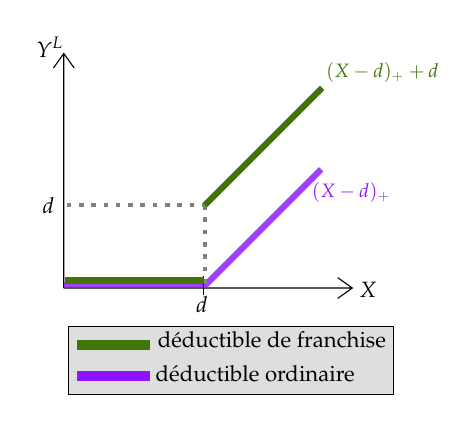
\begin{tikzpicture}[x=0.75pt,y=0.75pt,yscale=-1,xscale=1]
%uncomment if require: \path (0,253); %set diagram left start at 0, and has height of 253

%Shape: Axis 2D [id:dp399710789539935] 
\draw  (351.5,163) -- (490.5,163)(351.5,50) -- (351.5,163) -- cycle (483.5,158) -- (490.5,163) -- (483.5,168) (346.5,57) -- (351.5,50) -- (356.5,57)  ;
%Straight Lines [id:da18461968529502748] 
\draw [color={rgb, 255:red, 142; green, 19; blue, 254 }  ,draw opacity=0.82 ][line width=2.25]    (419,162.33) -- (475.5,105.83) ;
%Straight Lines [id:da11220757181905738] 
\draw [color={rgb, 255:red, 142; green, 19; blue, 254 }  ,draw opacity=0.82 ][line width=2.25]    (351.54,161.62) -- (419,161.62) ;
%Straight Lines [id:da8242096756691861] 
\draw [color={rgb, 255:red, 128; green, 128; blue, 128 }  ,draw opacity=1 ][line width=1.5]  [dash pattern={on 1.69pt off 2.76pt}]  (419.5,123) -- (419.5,161.62) ;
%Straight Lines [id:da1498600133265573] 
\draw    (419,166.33) -- (419,157.33) ;
%Straight Lines [id:da6809260076607797] 
\draw [color={rgb, 255:red, 128; green, 128; blue, 128 }  ,draw opacity=1 ][line width=1.5]  [dash pattern={on 1.69pt off 2.76pt}]  (352.83,123) -- (419.5,123) ;
%Straight Lines [id:da1340783435710058] 
\draw [color={rgb, 255:red, 65; green, 117; blue, 5 }  ,draw opacity=1 ][line width=2.25]    (351.88,159.33) -- (419,159.33) ;
%Straight Lines [id:da3630038280649066] 
\draw [color={rgb, 255:red, 65; green, 117; blue, 5 }  ,draw opacity=1 ][line width=2.25]    (419.5,123) -- (476,66.5) ;
%Shape: Rectangle [id:dp11226543371936115] 
\draw  [fill={rgb, 255:red, 222; green, 222; blue, 222 }  ,fill opacity=1 ] (353.75,181.33) -- (510.25,181.33) -- (510.25,214.33) -- (353.75,214.33) -- cycle ;
%Straight Lines [id:da23606671704725968] 
\draw [color={rgb, 255:red, 65; green, 117; blue, 5 }  ,draw opacity=1 ][line width=3.75]    (357.92,190.33) -- (393.25,190.33) ;
%Straight Lines [id:da48441164047430596] 
\draw [color={rgb, 255:red, 142; green, 19; blue, 254 }  ,draw opacity=1 ][line width=3.75]    (357.92,205.33) -- (393.25,205.33) ;


% Text Node
\draw (498,164) node  [font=\footnotesize] [align=left] {$\displaystyle X$};
% Text Node
\draw (490,117) node  [font=\scriptsize,color={rgb, 255:red, 144; green, 19; blue, 254 }  ,opacity=1 ] [align=left] {$\displaystyle ( X-d)_{+}$};
% Text Node
\draw (340,118) node [anchor=north west][inner sep=0.75pt]  [font=\footnotesize] [align=left] {$\displaystyle d$};
% Text Node
\draw (414,166) node [anchor=north west][inner sep=0.75pt]  [font=\footnotesize] [align=left] {$\displaystyle d$};
% Text Node
\draw (505,59) node  [font=\scriptsize,color={rgb, 255:red, 65; green, 117; blue, 5 }  ,opacity=1 ] [align=left] {$\displaystyle ( X-d)_{+} +d$};
% Text Node
\draw (345,47) node  [font=\footnotesize] [align=left] {$\displaystyle Y^{L}$};
% Text Node
\draw (443.75,204) node  [font=\small] [align=left] {{\footnotesize déductible ordinaire}};
% Text Node
\draw (451.75,188) node  [font=\small] [align=left] {{\footnotesize déductible de franchise}};


\end{tikzpicture}
\end{center}
\end{definitionNOHFILLsub}

\begin{definitionNOHFILLsub}[L'espérance du montant de perte avec un déductible de franchise]
\textbf{L'espérance du montant de perte}, pour l'assureur, \textbf{avec un déductible \textit{de franchise}} \lfbox[formula]{$\text{E}[X | X > d]$} correspond à :

\begin{align*}
	\text{E}[X | X > d]
	&=	\int_{d}^{\infty} x f(x) dx
	=	\int_{d}^{\infty} (x - d) f(x) dx + d \int_{d}^{\infty} f(x) dx \\
	&=	\text{E}[(X - d)_{+}] + dS(d)	 
\end{align*}
\end{definitionNOHFILLsub}


\subsubsection{Impacts du déductible sur la fréquence}
\textbf{Pour la classe $(a, b, 0)$ de distributions, on trouve les relations suivantes} :
\begin{center}
\begin{tabular}{| >{\columncolor{beaublue}}c | >{\columncolor{beaublue}}c  |}
\hline\rowcolor{airforceblue} 
\textcolor{white}{\textbf{Nombre de \textbf{pertes} ($N$)}}	&	\textcolor{white}{\textbf{Nombre de \textbf{paiements} ($N'$)}}		\\\specialrule{0.1em}{0em}{0em} 
$\text{Pois}(\lambda)$&	$\text{Pois}(S(d)\lambda)$	\\\hline
$\text{Binom}(n, p)$&	$\text{Binom}(n, S(d)p)$	\\\hline
$\text{BinNeg}(r, \beta)$&	$\text{BinNeg}(r, S(d)\beta)$	\\\hline
\end{tabular}
\end{center}



\columnbreak
\subsection{Coassurance}
\begin{definitionNOHFILL}[Coassurance $\alpha$]
Le pourcentage de coassurance \lfbox[formula]{$\alpha$} correspond à la portion de la perte payée par l'assureur. Pour une perte de $X$, l'assureur paye $\alpha X$ et l'assuré paye $(1 - \alpha)X$.

\begin{center}
\tikzset{every picture/.style={line width=0.75pt}} %set default line width to 0.75pt        
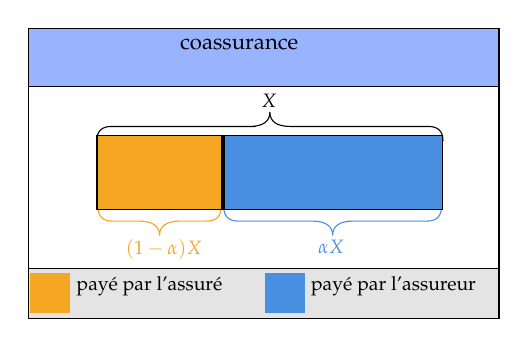
\begin{tikzpicture}[x=0.75pt,y=0.75pt,yscale=-1,xscale=1]
%uncomment if require: \path (0,217); %set diagram left start at 0, and has height of 217

%Shape: Rectangle [id:dp857212648137277] 
\draw  [fill={rgb, 255:red, 255; green, 255; blue, 255 }  ,fill opacity=1 ] (291,53.67) -- (517.8,53.67) -- (517.8,190) -- (291,190) -- cycle ;
%Shape: Rectangle [id:dp6577506986994079] 
\draw  [fill={rgb, 255:red, 228; green, 228; blue, 228 }  ,fill opacity=1 ] (291,169.41) -- (517.8,169.41) -- (517.8,193.67) -- (291,193.67) -- cycle ;
%Shape: Rectangle [id:dp10763459705704914] 
\draw  [fill={rgb, 255:red, 152; green, 180; blue, 255 }  ,fill opacity=1 ] (291,81.92) -- (517.8,81.92) -- (517.8,53.92) -- (291,53.92) -- cycle ;
%Shape: Rectangle [id:dp5604169395708387] 
\draw  [draw opacity=0][fill={rgb, 255:red, 245; green, 166; blue, 35 }  ,fill opacity=1 ] (292,171.41) -- (311.05,171.41) -- (311.05,191.08) -- (292,191.08) -- cycle ;
%Shape: Rectangle [id:dp8289199602562443] 
\draw  [draw opacity=0][fill={rgb, 255:red, 74; green, 144; blue, 226 }  ,fill opacity=1 ] (405.27,171.41) -- (424.32,171.41) -- (424.32,191.08) -- (405.27,191.08) -- cycle ;
%Shape: Brace [id:dp47861464036696866] 
\draw  [color={rgb, 255:red, 245; green, 166; blue, 35 }  ,draw opacity=1 ] (324.54,139.59) .. controls (324.54,144.26) and (326.87,146.59) .. (331.54,146.59) -- (344.24,146.59) .. controls (350.91,146.59) and (354.24,148.92) .. (354.24,153.59) .. controls (354.24,148.92) and (357.57,146.59) .. (364.24,146.59)(361.24,146.59) -- (376.94,146.59) .. controls (381.61,146.59) and (383.94,144.26) .. (383.94,139.59) ;
%Shape: Brace [id:dp08336874707524533] 
\draw  [color={rgb, 255:red, 74; green, 144; blue, 226 }  ,draw opacity=1 ] (385.2,139.59) .. controls (385.2,144.26) and (387.53,146.59) .. (392.2,146.59) -- (427.65,146.59) .. controls (434.32,146.59) and (437.65,148.92) .. (437.65,153.59) .. controls (437.65,148.92) and (440.98,146.59) .. (447.65,146.59)(444.65,146.59) -- (483.09,146.59) .. controls (487.76,146.59) and (490.09,144.26) .. (490.09,139.59) ;
%Shape: Rectangle [id:dp44830624755942683] 
\draw  [draw opacity=0][fill={rgb, 255:red, 74; green, 144; blue, 226 }  ,fill opacity=1 ] (384.8,105.33) -- (490.65,105.33) -- (490.65,140.85) -- (384.8,140.85) -- cycle ;
%Shape: Rectangle [id:dp597465273982372] 
\draw  [draw opacity=0][fill={rgb, 255:red, 245; green, 166; blue, 35 }  ,fill opacity=1 ] (324.15,105.33) -- (384.8,105.33) -- (384.8,140.85) -- (324.15,140.85) -- cycle ;
%Shape: Rectangle [id:dp062060105534497145] 
\draw   (324.15,105.33) -- (490.65,105.33) -- (490.65,140.85) -- (324.15,140.85) -- cycle ;
%Straight Lines [id:da8476063385253465] 
\draw [line width=1.5]    (384.8,105.33) -- (384.8,140.85) ;

%Shape: Brace [id:dp09659689837862229] 
\draw   (490.83,108) .. controls (490.83,103.33) and (488.5,101) .. (483.83,101) -- (417.42,101) .. controls (410.75,101) and (407.42,98.67) .. (407.42,94) .. controls (407.42,98.67) and (404.09,101) .. (397.42,101)(400.42,101) -- (331,101) .. controls (326.33,101) and (324,103.33) .. (324,108) ;

% Text Node
\draw (362.9,57.42) node [anchor=north west][inner sep=0.75pt]  [font=\large] [align=left] {{\footnotesize coassurance}};
% Text Node
\draw (313.05,171.81) node [anchor=north west][inner sep=0.75pt]   [align=left] {{\scriptsize payé par l'assuré}};
% Text Node
\draw (426.02,171.81) node [anchor=north west][inner sep=0.75pt]   [align=left] {{\scriptsize payé par l'assureur}};
% Text Node
\draw (429.36,154.31) node [anchor=north west][inner sep=0.75pt]  [font=\scriptsize] [align=left] {$\displaystyle \textcolor[rgb]{0.29,0.56,0.89}{\alpha X}$};
% Text Node
\draw (336.74,154.31) node [anchor=north west][inner sep=0.75pt]  [font=\scriptsize] [align=left] {$\displaystyle \textcolor[rgb]{0.96,0.65,0.14}{( 1-\alpha ) X}$};
% Text Node
\draw (402,84) node [anchor=north west][inner sep=0.75pt]  [font=\scriptsize] [align=left] {$\displaystyle X$};
\end{tikzpicture}
\end{center}
\end{definitionNOHFILL}

\begin{definitionNOHFILLsub}[L'espérance du montant de perte avec coassurance]
\textbf{L'espérance du montant de perte}, pour l'assureur, \textbf{avec une coassurance de $\alpha$} est \lfbox[formula]{$\text{E}[\alpha X]	=	\alpha \text{E}[X]$}.
\end{definitionNOHFILLsub}


\subsection{Combinaison des facteurs}
\textbf{Cas d'un déductible et de coassurance}
\begin{itemize}
	\item	Habituellement, la coassurance est appliquée \textit{\textbf{après}} le déductible et la perte pour l'assureur est :
		\begin{align*}
		Y^{L}
		&=	\begin{cases}
			0,	&	X \leq d	\\
			\alpha(X - d),	&	X > d
			\end{cases}	\\
		\text{E}[Y^{L}]	
		&=	\alpha\left(\text{E}[X]	-	\text{E}[X \wedge d]	\right)
		\end{align*}
	\item	Si une question spécifie que la coassurance s'applique \textit{\textbf{\textcolor{teal}{avant}}} le déductible, il suffit de remplacer $d$ par $\textcolor{teal}{\frac{d}{\alpha}}$ et mettre le $\alpha$ en évidence comme avant :
		\begin{align*}
		Y^{L}
		&=	\begin{cases}
			0,	&	\alpha X \leq d	\\
			\alpha X - d,	&	\alpha X > d
			\end{cases}	
		=	\begin{cases}
			0,	&	X \leq \textcolor{teal}{\frac{d}{\alpha}}	\\
			\alpha\left(X - \textcolor{teal}{\frac{d}{\alpha}}\right),	&	X > \textcolor{teal}{\frac{d}{\alpha}}
			\end{cases}	\\
		\text{E}[Y^{L}]	
		&=	\alpha\left(\text{E}[X]	-	\text{E}\left[X \wedge \textcolor{teal}{\frac{d}{\alpha}}\right]	\right)
		\end{align*}
\end{itemize}

Soit une police ayant : 
\begin{enumerate}
	\item	une coassurance de $\alpha$,
	\item	une limite de police de $u$,
	\item	un déductible \textit{\textbf{ordinaire}} de $d$.
\end{enumerate}

Alors, \lfbox[formula]{$\text{E}[Y^{L}]	=	\alpha \left\{\text{E}[X \wedge m]	-	\text{E}[X \wedge d]\right\}$} et 
\begin{align*}
	Y^{L}
	&=	\begin{cases}
		0, 	&	X \leq d	\\
		\alpha (X - d), 	&	d < X < m	\\
		u, 	&	X \geq m	
		\end{cases}
\end{align*}
où $m$ est la \textbf{perte maximale admissible}.

\begin{definitionNOHFILLprop}[Perte maximale admissible $m$]
Soit la perte maximale admissible \lfbox[formula]{$m	=	\frac{u}{\alpha} + d$} représentant la plus petite perte pour laquelle l'assureur paye la limite $u$.

\begin{itemize}
	\item	En anglais, \og \textit{maximum covered loss} \fg{}.
\end{itemize}
\end{definitionNOHFILLprop}

Visuellement : 
\begin{center}
\tikzset{every picture/.style={line width=0.75pt}} %set default line width to 0.75pt        
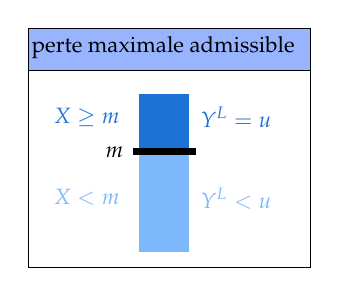
\begin{tikzpicture}[x=0.75pt,y=0.75pt,yscale=-1,xscale=1]
%uncomment if require: \path (0,155); %set diagram left start at 0, and has height of 155

%Shape: Rectangle [id:dp6067733498652601] 
\draw  [fill={rgb, 255:red, 255; green, 255; blue, 255 }  ,fill opacity=1 ] (100.5,13.18) -- (236.5,13.18) -- (236.5,128.67) -- (100.5,128.67) -- cycle ;
%Shape: Rectangle [id:dp4508485722610478] 
\draw  [draw opacity=0][fill={rgb, 255:red, 125; green, 183; blue, 252 }  ,fill opacity=1 ] (178.19,72.58) -- (178.19,121.06) -- (153.95,121.06) -- (153.95,72.58) -- cycle ;
%Shape: Rectangle [id:dp9575111659319537] 
\draw  [draw opacity=0][fill={rgb, 255:red, 29; green, 114; blue, 213 }  ,fill opacity=1 ] (178.19,44.81) -- (178.19,72.58) -- (153.95,72.58) -- (153.95,44.81) -- cycle ;
%Straight Lines [id:da9142966775592043] 
\draw [color={rgb, 255:red, 0; green, 0; blue, 0 }  ,draw opacity=1 ][line width=2.25]    (181.19,72.58) -- (150.99,72.58) ;

%Shape: Rectangle [id:dp3490985301668257] 
\draw  [fill={rgb, 255:red, 152; green, 180; blue, 255 }  ,fill opacity=1 ] (100.5,13.18) -- (236.5,13.18) -- (236.5,33.69) -- (100.5,33.69) -- cycle ;

% Text Node
\draw (101,15.93) node [anchor=north west][inner sep=0.75pt]  [font=\small] [align=left] {{\footnotesize perte maximale admissible}};
% Text Node
\draw (136.5,69.01) node [anchor=north west][inner sep=0.75pt]  [font=\footnotesize] [align=left] {$\displaystyle m$};
% Text Node
\draw (182.5,89.01) node [anchor=north west][inner sep=0.75pt]  [font=\footnotesize,color={rgb, 255:red, 125; green, 183; blue, 252 }  ,opacity=1 ] [align=left] {$\displaystyle Y^{L} < u$};
% Text Node
\draw (182.5,50.01) node [anchor=north west][inner sep=0.75pt]  [font=\footnotesize,color={rgb, 255:red, 29; green, 114; blue, 213 }  ,opacity=1 ] [align=left] {$\displaystyle Y^{L} =u$};
% Text Node
\draw (111.5,89.51) node [anchor=north west][inner sep=0.75pt]  [font=\footnotesize,color={rgb, 255:red, 125; green, 183; blue, 252 }  ,opacity=1 ] [align=left] {$\displaystyle X< m$};
% Text Node
\draw (111.5,50.51) node [anchor=north west][inner sep=0.75pt]  [font=\footnotesize,color={rgb, 255:red, 29; green, 114; blue, 213 }  ,opacity=1 ] [align=left] {$\displaystyle X\geq m$};
\end{tikzpicture}
\end{center}

%\begin{align*}
%Y^{(L\textcolor{blue}{|P)}}_{(O)} 
%	&=	\begin{cases}
%			(0 {\color{blue}{| \text{Non-défini})}},	&	\ x  < \frac{d}{1 + r} \\
%			\alpha \Big((1 + r) x - d \Big),	&	\ \frac{d}{1 + r} \leq x < \frac{u}{1 + r} \\
%			\alpha (u - d),	&	\ x \geq \frac{u}{1 + r} \\
%		\end{cases}	\\
%	\esp{Y^{(L\textcolor{blue}{|P)}}_{(O)}} 
%	&=	\frac{\alpha (1 + r) \left( 
%			\text{E}\left[X \wedge \frac{u}{1 + r}\right] -  
%			\text{E}\left[X \wedge \frac{d}{1 + r}\right]  
%		\right)}{{\color{blue}{S_{X} \left(\frac{d}{1 + r}\right)}}} 
%\end{align*}


\columnbreak
\subsection{Inflation}
\begin{definitionNOHFILL}[Inflation $r$]
L'inflation de \lfbox[formula]{$r$} augmente les coûts, mais, de façon générale, ils sont couverts par la compagnie d'assurance et ne causent pas de changements à la police.
\end{definitionNOHFILL}

\begin{definitionNOHFILLsub}[L'espérance du montant de perte avec inflation]
\textbf{L'espérance du montant de perte}, pour l'assureur, \textbf{avec de l'inflation de $r$} est \lfbox[formula]{$\text{E}[(1 + r) X]	=	(1 + r) \text{E}[X]$}.\\

Combiné avec les autres facteurs :

\begin{align*}
	\text{E}\left[Y^{L}\right]		
	&=	\alpha(1 + r) \left(\text{E}\left[X \wedge \frac{m}{1 + r}\right]	-	\text{E}\left[X \wedge \frac{d}{1 + r}\right]\right)	\\
	\text{E}\left[Y^{P}\right]	
	&=	\frac{\text{E}[Y^{L}]}{S_{X}\left(\frac{d}{1 + r}\right)}
\end{align*}
\end{definitionNOHFILLsub}

\paragraph{Note}	Si la distribution de $X$ comporte un paramètre d'échelle $\theta$, on peut simplifier les équations en posant \lfbox[formula]{$\theta'	=	(1 + r)\theta$}.



\pagebreak
\section{Estimation de modèles non paramétriques}
\subsection{Données complètes}
\hl{Section à compléter avec mes notes d’ IARD et 11.2 de Nonlife Actuariel Models (tse).}
\subsubsection{Distribution empirique}
\begin{definitionNOHFILL}[Distribution empirique]
Distribution discrète prenant comme valeurs $y_{1}, \dots, y_{m}$ avec probabilités $\frac{w_{1}}{n}, \dots, \frac{w_{m}}{n}$;
\begin{itemize}
	\item	On peut également la définir comme la distribution discrète équiprobable des valeurs $x_{1}, \dots, x_{n}$.
\end{itemize}
\end{definitionNOHFILL}

\begin{distributions}[Notation]
\begin{description}
	\item[$\hat{f}()$]	Fonction de densité empirique.	
	\item[$\hat{F}()$]	Fonction de répartition empirique.	
	\item[$\tilde{F}()$]	Fonction de répartition lissée;
		\begin{itemize}
		\item	En anglais, \og \textit{smoothed empirical distribution function} \fg{}.
		\item	On appelle parfois la fonction de répartition \textit{la fonction distribution} (\og \textit{distribution function} \fg{}).
		\end{itemize}
%	\item[Moyenne de la distribution empirique]
%		\begin{align*}
%		\sumz{m}{j = 1} \frac{w_{j}}{n} y_{j}
%		&=	\frac{1}{n} \sumz{n}{i = 1} x_{i}
%		\end{align*}
%	\item[Variance de la distribution empirique]
%		\begin{align*}
%		\sumz{m}{j = 1} \frac{w_{j}}{n} (y_{j} - \bar{x})^{2}
%		&=	\frac{1}{n} \sumz{n}{i = 1} (y_{i} - \bar{x})^{2}
%		\end{align*}
\end{description}
\end{distributions}

\begin{align*}
	\hat{f}(y)
	&=	\begin{cases}
		\frac{w_{j}}{n},	&	\text{si } y = y_{j} \, \forall j	\\
		0,	&	\text{sinon}
		\end{cases}	\\
		\hat{F}(y)
	&=	\begin{cases}
		0,	&	y	<	y_{1},	\\
		\frac{1}{n}\sumz{j}{h = 1}w_{h},	&	y_{j}	\leq	y	<	y_{j + 1}, \, j	=	1, \dots, m - 1	\\
		1,	&	y_{m}	\leq	y
		\end{cases}
\end{align*}		

On peut estimer la valeur de $\hat{F}()$ pour un une valeur de $y$ pas dans l'ensemble $y_{1}, \dots, y_{m}$ avec la fonction de répartition lissée $\tilde{F}()$. Pour \icbox[red][palechestnut]{$y_{j} \leq y < y_{j + 1}$} et \icbox[red][palechestnut]{$j \in \{1, 2, \dots, m - 1\}$}, $\tilde{F}(y)$ est une interpolation linéaire de $\hat{F}(y_{j + 1})$ et $\hat{F}(y_{j})$ :
\begin{align*}
	\tilde{F}(y)
	&=	\frac{y	-	y_{j	}}{y_{j + 1}	-	y_{j}}\hat{F}(y_{j + 1})  + 
		\frac{y_{j + 1}	-	y_{j	}}{y_{j + 1}	-	y_{j}}\hat{F}(y_{j})
\end{align*}

\begin{definitionNOHFILLprop}[Distribution binomiale de la fonction de répartition empirique]
On peut écrire la fonction de répartition empirique comme \lfbox[formula]{$\hat{F}(y)	=	\frac{Y}{n}$} où $Y$ est le nombre d'observations qui sont inférieures ou égales à $y$ tel que \lfbox[formula]{$Y \sim \text{Bin}(n, p = F(y))$}.\\

On trouve :
\begin{align*}
	\text{E}[Y]	
	&=	\frac{\text{E}[\hat{F}(y)]}{n}
	=	F(y)		\\
	\text{Var}(Y)
	&=	\frac{\text{Var}(\hat{F}(y))}{n^{2}}
	=	\frac{F(y)(1 - F(y))}{n}
\end{align*}
\end{definitionNOHFILLprop}


\subsubsection{Estimation par noyaux}
La fonction de répartition empirique résume les données d'une distribution discrète. Cependant, lorsque la variable d'intérêt $X$ est continue on souhaite estimer une fonction de densité.

Pour une observation $x_{i}$ de l'échantillon, la fonction de répartition empirique assigne une masse de probabilité de $1/n$ au point $x_{i}$.
Puisque $X$ est continue, il est normal que l'on souhaite \underline{\textit{distribuer}} cette masse \textit{autour} de $x_{i}$.

Si l'on souhaite distribuer cette masse de façon égale, on le fait sur l'intervalle \icbox{$[x_{i}  - b, x_{i} + b]$} avec la fonction de $x_{i}$ $f_{i}(x)$:
\begin{align*}
	f_{i}(x)
	&=	\begin{cases}
		\frac{0.5}{b},	&	x_{i} - b	\leq		x	\leq		x_{i} + b,	\\
		0,	&	\text{sinon}
		\end{cases}	
\end{align*}
\begin{itemize}[leftmargin = *]
	\item	Cette fonction est rectangulaire avec une base de longueur $2b$ et une hauteur de $0.5/b$ pour avoir une aire de 1.
	\item	On peut l'interpréter comme la fonction de densité contribuée par l'observation $x_{i}$;
	\item	On note que ceci correspond à la fonction de densité d'une distribution uniforme $U(x_{i} -  b, x_{i} + b)$;
	\item	Alors, seulement les valeurs de $x$ contenues dans l'intervalle $(x_{i} -  b, x_{i} + b)$ reçoivent une "contribution" de $x_{i}$;
	\item	La fonction de densité de $X$ est donc la somme des masses de probabilité contribuées \icbox[red][palechestnut]{$\tilde{f}(x)	=	\frac{1}{n} \sumz{n}{i = 1}(x)$}.
\end{itemize}

On défini $\phi_{i}	=	\frac{x - x_{i}}{b}$ et $K_{R}(\phi)$:
\begin{align*}
	K_{R}(\phi)
	&=	\begin{cases}
		\frac{1}{2},	&	-1	\leq		\phi	\leq		1,	\\
		0,	&	\text{sinon}
		\end{cases}	
\end{align*}
\begin{itemize}[leftmargin = *]
	\item	On trouve donc que \icbox[red][palechestnut]{$f_{i}(x)	=	\frac{1}{b}K_{R}(\phi_{i})$} et \icbox[red][palechestnut]{$\tilde{f}(x)	=	\frac{1}{nb}\sumz{n}{i = 1}K_{R}(\phi_{i})$}.
\end{itemize}

\begin{distributions}[Notation]
\begin{description}
	\item[$b$]	\og \textit{bandwith} \fg{} où \icbox[red][palechestnut]{$b > 0$};
	\item[$K_{R}(\phi)$]	\og \textit{rectangular (box, uniform) kernel function} \fg{};
	\item[$\tilde{f}(x)$]	Estimation de la fonction de densité selon le noyau rectangulaire;
	\item[$K_{T}(\phi)$]	\og \textit{triangular kernel} \fg{};
	\begin{align*}
		K_{R}(\phi)
		&=	\begin{cases}
			1 - |\phi|,	&	-1	\leq		\phi	\leq		1,	\\
			0,	&	\text{sinon}
			\end{cases}	
	\end{align*}
	\item[$K_{G}(\phi)$]	\og \textit{Gaussian kernel} \fg{};
		\begin{align*}
		K_{G}(\phi)
		&=	\frac{1}{\sqrt{2\pi}} \textrm{e}^{-\frac{\phi^{2}}{2}}, -\infty	<	\phi	<	\infty
		\end{align*}
\end{description}
\end{distributions}




\columnbreak
\subsection{Données incomplètes}
\hl{Section à compléter avec mes notes d’ IARD et 11.2 de Nonlife Actuariel Models (tse).}
\subsubsection{Estimateur de Kaplan-Meier}
Soit : 
\begin{align*}
	S(y_{j})
	&=	\Pr(X > y_{1})	\Pr(X > y_{2} | X > y_{1}) \hdots \Pr(X > y_{j} | X > y_{j - 1})
	=	\Pr(X > y_{1}) \prod_{h = 2}^{j} \Pr(X > y_{h} | X > y_{h - 1})
\end{align*}

Où on peut estimer $\widehat{\Pr}(X > y_{1})	=	1	-	\frac{w_{1}}{r_{1}}$ et $\widehat{\Pr}(X > y_{h} | X > y_{h - 1})	=	1	-	\frac{w_{h}}{r_{h}}$ pour \lfbox[conditions]{$h	=	2, \dots, m$}.

Il s'ensuit qu'on peut estimer $S(y_{j})$ par :
\begin{align*}
	\hat{S}(y_{j})
	&=	\prod_{h = 1}^{j} \left(1 - \frac{w_{h}}{r_{h}}\right)
\end{align*}

Variance de l'estimateur Kaplan-Meier : \lfbox[formula]{$\text{Var}(\hat{S}_{K}(y_{j}) | \mathcal{C})	\approx	\left(S(y_{j})\right)^{2} \left(\sum^{j}_{h = 1} \frac{1 - S_{h}}{S_{h}r_{h}}\right)$} 
Approximation de Greenwood de la variance de l'estimateur Kaplan-Meier : \lfbox[formula]{$\widehat{\text{Var}}(\hat{S}_{K}(y_{j}) | \mathcal{C})	\approx	\left(\hat{S}_{K}(y_{j})\right)^{2} \left(\sum^{j}_{h = 1} \frac{w_{h}}{r_{h} (r_{h} - w_{h})}\right)$} 


\subsubsection{Estimateur de Nelson-Aalen}
\begin{distributions}[Notation]
\begin{description}
	\item[$h(y)$]	Fonction de hasard.
	\item[$H(y)$]	Fonction de hasard cumulative.
\end{description}
\end{distributions} 

\begin{align*}
	H(y)
	&=	\int_{0}^{y} h(y) dy
\end{align*}

Il s'ensuit que \lfbox[formula]{$S(y)	=	\textrm{e}^{-H(y)}$} et \lfbox[formula]{$H(y)	=	-\ln\left(S(y)\right)$}.

Avec l'approximation \lfbox[conditions]{$-\ln\left(1	-	\frac{w_{h}}{r_{h}}\right)	\approx	\frac{w_{h}}{r_{h}}$} on trouve que \lfbox[formula]{$H(y)	=	\sum_{h	=	1}^{j} \frac{w_{h}}{r_{h}}$} qui correspond à l'\textbf{estimateur Nelson-Aalen} de la fonction de hasard cumulative.

\columnbreak
\subsection{Données groupées}
\hl{Section à compléter avec mes notes d’ IARD et 11.3 de Nonlife Actuariel Models (tse).}



\pagebreak
\section{Estimation de modèles paramétriques}
\subsection*{Estimation par maximum de vraisemblance pour des données incomplètes et groupées}
Lorsque les données sont groupées et/ou incomplètes, les observations ne sont plus iid, mais on peut quand même formuler la fonction de vraisemblance et trouver l'EMV.

La première étape est d'écrire la fonction de (log) vraisemblance adéquate pour la méthode d'échantillonnage des données.\\

Par exemple, soit des données groupées en $k$ intervalles : 
\begin{itemize}
	\item	On trouve avec la fonction de répartition $F(\cdot; \theta)$ que la probabilité d'être dans l'intervalle $(c_{j - 1}, c_{j}]$ est $F(c_{j}; \theta)	-	F(c_{j - 1}; \theta)$;
	\item	On pose que les observations individuelles sont iid;
	\item	Donc, la vraisemblance d'avoir $n_{j}$ observations dans l'intervalle $(c_{j - 1}, c_{j}]$, \lfbox[conditions]{pour $j	=	1, \dots, k$ et $\bm{n}	=	(n_{1}, \cdots, n_{k})$} est :
		\begin{align*}
		\mathcal{L}(\theta; \bm{n})
		&=	\prod^{k}_{j	=	1} \left[F(c_{j}; \theta)	-	F(c_{j - 1}; \theta)\right]^{n_{j}}
		\end{align*}
\end{itemize}


\setlength{\mathindent}{-0.75cm}
\subsection{Fonction de vraisemblance}
\begin{definitionNOHFILLprop}[Données complètes]
\begin{align*}
	\mathcal{L}(\theta; \bm{x})
	&=	\prod^{k}_{j	=	1} \underbrace{f(x_{j}; \theta)}_{\substack{\text{probabilité que chaque}\\ \text{observation soit égale à}\\ \text{la valeur observée}}}
\end{align*}
\end{definitionNOHFILLprop}

\begin{definitionNOHFILLprop}[Données groupées en $k$ intervalles]
\begin{align*}
	\mathcal{L}(\theta; \bm{x})
	&=	\prod^{k}_{j	=	1} \underbrace{\left[F(c_{j}; \theta)	-	F(c_{j - 1}; \theta)\right]^{n_{j}}}_{\substack{\text{probabilité qu'une observation}\\ \text{soit contenue dans l'intervalle}}}
\end{align*}
\end{definitionNOHFILLprop}

\begin{definitionNOHFILLprop}[Données censurées vers la droite]
On pose que $n_{1}$ observations sont complètes et que $n_{2}$ observations sont censurées à la limite de $u$ :
\begin{align*}
	\mathcal{L}(\theta; \bm{x})
	&=	\underbrace{\left[\prod^{n_{1}}_{i	=	1} f(x_{i}; \theta) \right]}_{\shortstack{probabilité de chaque\\ observation à la\\ valeur observée}} \overbrace{\left[1	-	F(u; \theta)\right]^{n_{2}}}^{\substack{\text{probabilité qu'une observation}\\ \text{soit supérieure, ou égale, à $u$}}}
\end{align*}
\end{definitionNOHFILLprop}

\begin{definitionNOHFILLprop}[tronquées vers la gauche]
On pose un déductible de $d$ : 
\begin{align*}
	\mathcal{L}(\theta; \bm{x})
	&=	\underbrace{\frac{1}{\left[1	-	F(d; \theta)\right]^{n}}}_{\substack{\text{pondère la vraisemblance par}\\ \text{la probabilité d'être supérieur}\\ \text{au déductible}}} \prod^{n}_{i	=	1} f(x_{i}; \theta)
\end{align*}
\end{definitionNOHFILLprop}



\pagebreak
\section{Évaluation et sélection de modèles}
\hl{Cette section n'est pas suffisamment bien expliquée pour que je la considère complète.}\\
\begin{rappel_enhanced}[Contexte]
Évaluer les modèles avec des méthodes non paramétriques a l'avantage d'avoir très peu d'hypothèses. Cependant, il est plus difficile d'évaluer le modèle d'un point de vue théorique.

Évaluer les modèles avec des méthodes paramétriques a l'avantage de résumer le modèle à un petit nombre de paramètres. Cependant, ces méthodes sont une simplification et risquent d'imposer la mauvaise structure.
\end{rappel_enhanced}

\subsection{Graphiquement}
Avec les méthodes d'évaluation visuelles, on peut détecter si les données diffèrent anormalement du modèle paramétrique.
\begin{itemize}
	\item	On peut évaluer la fonction de répartition empirique et la fonction de répartition théorique sur un même graphique pour évaluer l'ajustement.
	\item	On peut évaluer le tracé des probabilités (\og \textit{P-P plot} \fg{}) qui trace la répartition empirique et la répartition théorique.
	\item	On peut tracer l'histogramme des données et superposer la densité théorique pour évaluer l'ajustement.
\end{itemize}

Le désavantage de ces méthodes est qu'elles ne fournissent pas des mesures quantitatives sur l'ajustement du modèle.


\subsection{Tests pour la qualité de l'ajustement}
\begin{definitionNOHFILL}[Tests de spécification (\og \textit{misspecification tests} \fg{})]
Test de signifiance dont l'objectif est d'évaluer les hypothèses de distribution d'un modèle.

\end{definitionNOHFILL}

\begin{distributions}[Notation]
\begin{description}
	\item[$F^{\ast}()$]	Fonction de répartition d'une v.a. continue (hypothèse nulle).
	\item[$\hat{F}()$]	Fonction de répartition empirique.
\end{description}
\end{distributions}

Les tests de Kolmogorov-Smirnov (K.-S.) et de Anderson-Darling sont idéaux lorsque l'on désire comparer les fonctions de répartition. \\

Le test de K.-S. compare la fonction de distribution (répartition) empirique à celle d'une distribution théorique. L'idée du test est donc de quantifier l'évaluation visuelle que l'on peut faire de l'ajustement.

\begin{definitionNOHFILLsub}[Test de Kolmogorov-Smirnov]
On teste si les données semblent suivre une distribution (« supportent l'hypothèse nulle ») avec la statistique de Kolmogorov-Smirnov : \lfbox[formula]{$D	=	\underset{x_{(1)}	\leq	x	\leq	x_{(n)}}{\max} \left| \hat{F}(x)	-	F^{\ast}(x) \right|$}.
\begin{itemize}
	\item	Ceci équivaut donc à calculer la différence maximale entre la fonction de répartition empirique et celle de la distribution.
	\item	Puisque $\hat{F}()$ est une fonction à escalier, il faut seulement évaluer la fonction aux points observés $x_{(1)}	\leq	x_{(2)}	\leq	\hdots	\leq	x_{(n)}$.
%%%	------------------------
%%%	NOTES
%%%	+	why?
%%%	------------------------
	\item	De plus, le maximum peut seulement arriver soit au point de saut $x_{(i)}$ ou immédiatement avant $x_{(i - 1)}$.
\end{itemize}

On peut donc récrire\\ \lfbox[formula]{$D	=	\underset{i \in \{1, \dots, n\}}{\max}\left\{ \max\left\{\left| \hat{F}(x_{(i - 1)})	-	F^{\ast}(x_{(i)}) \right|, \left| \hat{F}(x_{(i)})	-	F^{\ast}(x_{(i)}) \right|\right\}\right\}$}.

\begin{itemize}
	\item	Si les données sont bien ajustées, on s'attend à ce que $D$ soit très petit.
	\item	Lorsque la distribution est entièrement spécifiée (aucun paramètre n’est estimé), une table avec les valeurs critiques est donnée.
	\item	S'il faut estimer des paramètres, la simulation Monte-Carlo est utilisée pour trouver des nouvelles valeurs critiques.
\end{itemize}
\end{definitionNOHFILLsub}

\begin{definitionNOHFILLprop}[Test de K.-S. pour des données incomplètes]
Pour des données tronquées à $d$ et censurée (vers la droite) à $u$, \lfbox[formula]{$D	=	\underset{d	\leq	x	\leq	u}{\max} \left| \hat{F}(x)	-	F^{\ast}(x) \right|$}
\end{definitionNOHFILLprop}

Visuellement, le test de K.-S. ressemble à :
\begin{center}
\tikzset{every picture/.style={line width=0.75pt}} %set default line width to 0.75pt        

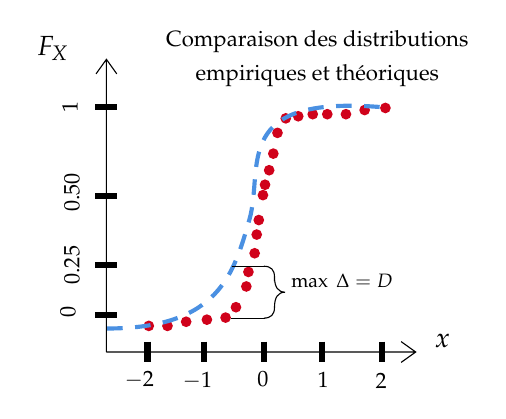
\begin{tikzpicture}[x=0.75pt,y=0.75pt,yscale=-1,xscale=1]
%uncomment if require: \path (0,300); %set diagram left start at 0, and has height of 300

%Shape: Axis 2D [id:dp24483060574985016] 
\draw  (159.17,162) -- (308.17,162)(159.17,21) -- (159.17,162) -- cycle (301.17,157) -- (308.17,162) -- (301.17,167) (154.17,28) -- (159.17,21) -- (164.17,28)  ;
%Straight Lines [id:da6030801017105296] 
\draw [line width=2.25]    (179,157) -- (179,167) ;
%Straight Lines [id:da2652234915508369] 
\draw [line width=2.25]    (206,157) -- (206,167) ;
%Straight Lines [id:da7718269955671673] 
\draw [line width=2.25]    (235,157) -- (235,167) ;
%Straight Lines [id:da8049939015901117] 
\draw [line width=2.25]    (263,157) -- (263,167) ;
%Straight Lines [id:da5692977431446764] 
\draw [line width=2.25]    (292,157) -- (292,167) ;
%Straight Lines [id:da036135237157260525] 
\draw [line width=2.25]    (153.67,44) -- (164.5,44) ;
%Straight Lines [id:da021466328536539292] 
\draw [line width=2.25]    (153.67,87) -- (164.5,87) ;
%Straight Lines [id:da8388615672035813] 
\draw [line width=2.25]    (153.67,120) -- (164.5,120) ;
%Straight Lines [id:da4377316999274832] 
\draw [line width=2.25]    (153.67,144) -- (164.5,144) ;
%Flowchart: Connector [id:dp27902589825476154] 
\draw  [draw opacity=0][fill={rgb, 255:red, 208; green, 2; blue, 27 }  ,fill opacity=1 ] (186,149.42) .. controls (186,147.99) and (187.16,146.83) .. (188.58,146.83) .. controls (190.01,146.83) and (191.17,147.99) .. (191.17,149.42) .. controls (191.17,150.84) and (190.01,152) .. (188.58,152) .. controls (187.16,152) and (186,150.84) .. (186,149.42) -- cycle ;
%Flowchart: Connector [id:dp8858881991629384] 
\draw  [draw opacity=0][fill={rgb, 255:red, 208; green, 2; blue, 27 }  ,fill opacity=1 ] (177,149.42) .. controls (177,147.99) and (178.16,146.83) .. (179.58,146.83) .. controls (181.01,146.83) and (182.17,147.99) .. (182.17,149.42) .. controls (182.17,150.84) and (181.01,152) .. (179.58,152) .. controls (178.16,152) and (177,150.84) .. (177,149.42) -- cycle ;
%Flowchart: Connector [id:dp965947428222834] 
\draw  [draw opacity=0][fill={rgb, 255:red, 208; green, 2; blue, 27 }  ,fill opacity=1 ] (195,147.42) .. controls (195,145.99) and (196.16,144.83) .. (197.58,144.83) .. controls (199.01,144.83) and (200.17,145.99) .. (200.17,147.42) .. controls (200.17,148.84) and (199.01,150) .. (197.58,150) .. controls (196.16,150) and (195,148.84) .. (195,147.42) -- cycle ;
%Flowchart: Connector [id:dp5208785016321031] 
\draw  [draw opacity=0][fill={rgb, 255:red, 208; green, 2; blue, 27 }  ,fill opacity=1 ] (205,146.42) .. controls (205,144.99) and (206.16,143.83) .. (207.58,143.83) .. controls (209.01,143.83) and (210.17,144.99) .. (210.17,146.42) .. controls (210.17,147.84) and (209.01,149) .. (207.58,149) .. controls (206.16,149) and (205,147.84) .. (205,146.42) -- cycle ;
%Flowchart: Connector [id:dp2872263470627334] 
\draw  [draw opacity=0][fill={rgb, 255:red, 208; green, 2; blue, 27 }  ,fill opacity=1 ] (214,145.42) .. controls (214,143.99) and (215.16,142.83) .. (216.58,142.83) .. controls (218.01,142.83) and (219.17,143.99) .. (219.17,145.42) .. controls (219.17,146.84) and (218.01,148) .. (216.58,148) .. controls (215.16,148) and (214,146.84) .. (214,145.42) -- cycle ;
%Flowchart: Connector [id:dp6170797725926003] 
\draw  [draw opacity=0][fill={rgb, 255:red, 208; green, 2; blue, 27 }  ,fill opacity=1 ] (219,140.42) .. controls (219,138.99) and (220.16,137.83) .. (221.58,137.83) .. controls (223.01,137.83) and (224.17,138.99) .. (224.17,140.42) .. controls (224.17,141.84) and (223.01,143) .. (221.58,143) .. controls (220.16,143) and (219,141.84) .. (219,140.42) -- cycle ;
%Flowchart: Connector [id:dp6321853947189746] 
\draw  [draw opacity=0][fill={rgb, 255:red, 208; green, 2; blue, 27 }  ,fill opacity=1 ] (224,130.42) .. controls (224,128.99) and (225.16,127.83) .. (226.58,127.83) .. controls (228.01,127.83) and (229.17,128.99) .. (229.17,130.42) .. controls (229.17,131.84) and (228.01,133) .. (226.58,133) .. controls (225.16,133) and (224,131.84) .. (224,130.42) -- cycle ;
%Flowchart: Connector [id:dp4527459516123209] 
\draw  [draw opacity=0][fill={rgb, 255:red, 208; green, 2; blue, 27 }  ,fill opacity=1 ] (225,123.42) .. controls (225,121.99) and (226.16,120.83) .. (227.58,120.83) .. controls (229.01,120.83) and (230.17,121.99) .. (230.17,123.42) .. controls (230.17,124.84) and (229.01,126) .. (227.58,126) .. controls (226.16,126) and (225,124.84) .. (225,123.42) -- cycle ;
%Flowchart: Connector [id:dp5990586632002524] 
\draw  [draw opacity=0][fill={rgb, 255:red, 208; green, 2; blue, 27 }  ,fill opacity=1 ] (228,114.42) .. controls (228,112.99) and (229.16,111.83) .. (230.58,111.83) .. controls (232.01,111.83) and (233.17,112.99) .. (233.17,114.42) .. controls (233.17,115.84) and (232.01,117) .. (230.58,117) .. controls (229.16,117) and (228,115.84) .. (228,114.42) -- cycle ;
%Flowchart: Connector [id:dp46008272444906795] 
\draw  [draw opacity=0][fill={rgb, 255:red, 208; green, 2; blue, 27 }  ,fill opacity=1 ] (229,105.42) .. controls (229,103.99) and (230.16,102.83) .. (231.58,102.83) .. controls (233.01,102.83) and (234.17,103.99) .. (234.17,105.42) .. controls (234.17,106.84) and (233.01,108) .. (231.58,108) .. controls (230.16,108) and (229,106.84) .. (229,105.42) -- cycle ;
%Flowchart: Connector [id:dp10208355949407677] 
\draw  [draw opacity=0][fill={rgb, 255:red, 208; green, 2; blue, 27 }  ,fill opacity=1 ] (243,49.42) .. controls (243,47.99) and (244.16,46.83) .. (245.58,46.83) .. controls (247.01,46.83) and (248.17,47.99) .. (248.17,49.42) .. controls (248.17,50.84) and (247.01,52) .. (245.58,52) .. controls (244.16,52) and (243,50.84) .. (243,49.42) -- cycle ;
%Flowchart: Connector [id:dp44081367516766856] 
\draw  [draw opacity=0][fill={rgb, 255:red, 208; green, 2; blue, 27 }  ,fill opacity=1 ] (249,48.42) .. controls (249,46.99) and (250.16,45.83) .. (251.58,45.83) .. controls (253.01,45.83) and (254.17,46.99) .. (254.17,48.42) .. controls (254.17,49.84) and (253.01,51) .. (251.58,51) .. controls (250.16,51) and (249,49.84) .. (249,48.42) -- cycle ;
%Flowchart: Connector [id:dp258791942489629] 
\draw  [draw opacity=0][fill={rgb, 255:red, 208; green, 2; blue, 27 }  ,fill opacity=1 ] (256,47.42) .. controls (256,45.99) and (257.16,44.83) .. (258.58,44.83) .. controls (260.01,44.83) and (261.17,45.99) .. (261.17,47.42) .. controls (261.17,48.84) and (260.01,50) .. (258.58,50) .. controls (257.16,50) and (256,48.84) .. (256,47.42) -- cycle ;
%Flowchart: Connector [id:dp7461727454132954] 
\draw  [draw opacity=0][fill={rgb, 255:red, 208; green, 2; blue, 27 }  ,fill opacity=1 ] (230,98.42) .. controls (230,96.99) and (231.16,95.83) .. (232.58,95.83) .. controls (234.01,95.83) and (235.17,96.99) .. (235.17,98.42) .. controls (235.17,99.84) and (234.01,101) .. (232.58,101) .. controls (231.16,101) and (230,99.84) .. (230,98.42) -- cycle ;
%Flowchart: Connector [id:dp3590383056585824] 
\draw  [draw opacity=0][fill={rgb, 255:red, 208; green, 2; blue, 27 }  ,fill opacity=1 ] (232,86.42) .. controls (232,84.99) and (233.16,83.83) .. (234.58,83.83) .. controls (236.01,83.83) and (237.17,84.99) .. (237.17,86.42) .. controls (237.17,87.84) and (236.01,89) .. (234.58,89) .. controls (233.16,89) and (232,87.84) .. (232,86.42) -- cycle ;
%Flowchart: Connector [id:dp1884350833419266] 
\draw  [draw opacity=0][fill={rgb, 255:red, 208; green, 2; blue, 27 }  ,fill opacity=1 ] (233,81.42) .. controls (233,79.99) and (234.16,78.83) .. (235.58,78.83) .. controls (237.01,78.83) and (238.17,79.99) .. (238.17,81.42) .. controls (238.17,82.84) and (237.01,84) .. (235.58,84) .. controls (234.16,84) and (233,82.84) .. (233,81.42) -- cycle ;
%Flowchart: Connector [id:dp24880669696449487] 
\draw  [draw opacity=0][fill={rgb, 255:red, 208; green, 2; blue, 27 }  ,fill opacity=1 ] (235,74.42) .. controls (235,72.99) and (236.16,71.83) .. (237.58,71.83) .. controls (239.01,71.83) and (240.17,72.99) .. (240.17,74.42) .. controls (240.17,75.84) and (239.01,77) .. (237.58,77) .. controls (236.16,77) and (235,75.84) .. (235,74.42) -- cycle ;
%Flowchart: Connector [id:dp23618438280038845] 
\draw  [draw opacity=0][fill={rgb, 255:red, 208; green, 2; blue, 27 }  ,fill opacity=1 ] (237,66.42) .. controls (237,64.99) and (238.16,63.83) .. (239.58,63.83) .. controls (241.01,63.83) and (242.17,64.99) .. (242.17,66.42) .. controls (242.17,67.84) and (241.01,69) .. (239.58,69) .. controls (238.16,69) and (237,67.84) .. (237,66.42) -- cycle ;
%Flowchart: Connector [id:dp38788335050603684] 
\draw  [draw opacity=0][fill={rgb, 255:red, 208; green, 2; blue, 27 }  ,fill opacity=1 ] (239,56.42) .. controls (239,54.99) and (240.16,53.83) .. (241.58,53.83) .. controls (243.01,53.83) and (244.17,54.99) .. (244.17,56.42) .. controls (244.17,57.84) and (243.01,59) .. (241.58,59) .. controls (240.16,59) and (239,57.84) .. (239,56.42) -- cycle ;
%Flowchart: Connector [id:dp8001516680880116] 
\draw  [draw opacity=0][fill={rgb, 255:red, 208; green, 2; blue, 27 }  ,fill opacity=1 ] (272,47.42) .. controls (272,45.99) and (273.16,44.83) .. (274.58,44.83) .. controls (276.01,44.83) and (277.17,45.99) .. (277.17,47.42) .. controls (277.17,48.84) and (276.01,50) .. (274.58,50) .. controls (273.16,50) and (272,48.84) .. (272,47.42) -- cycle ;
%Flowchart: Connector [id:dp06230967753042438] 
\draw  [draw opacity=0][fill={rgb, 255:red, 208; green, 2; blue, 27 }  ,fill opacity=1 ] (263,47.42) .. controls (263,45.99) and (264.16,44.83) .. (265.58,44.83) .. controls (267.01,44.83) and (268.17,45.99) .. (268.17,47.42) .. controls (268.17,48.84) and (267.01,50) .. (265.58,50) .. controls (264.16,50) and (263,48.84) .. (263,47.42) -- cycle ;
%Flowchart: Connector [id:dp4843810494735361] 
\draw  [draw opacity=0][fill={rgb, 255:red, 208; green, 2; blue, 27 }  ,fill opacity=1 ] (281,45.42) .. controls (281,43.99) and (282.16,42.83) .. (283.58,42.83) .. controls (285.01,42.83) and (286.17,43.99) .. (286.17,45.42) .. controls (286.17,46.84) and (285.01,48) .. (283.58,48) .. controls (282.16,48) and (281,46.84) .. (281,45.42) -- cycle ;
%Flowchart: Connector [id:dp9279424690148039] 
\draw  [draw opacity=0][fill={rgb, 255:red, 208; green, 2; blue, 27 }  ,fill opacity=1 ] (291,44.42) .. controls (291,42.99) and (292.16,41.83) .. (293.58,41.83) .. controls (295.01,41.83) and (296.17,42.99) .. (296.17,44.42) .. controls (296.17,45.84) and (295.01,47) .. (293.58,47) .. controls (292.16,47) and (291,45.84) .. (291,44.42) -- cycle ;
%Curve Lines [id:da002395199379529034] 
\draw [color={rgb, 255:red, 74; green, 144; blue, 226 }  ,draw opacity=1 ][line width=1.5]  [dash pattern={on 5.63pt off 4.5pt}]  (159.5,150.67) .. controls (213.5,150.67) and (220.5,124.17) .. (228,98.42) .. controls (235.5,72.67) and (217.5,36.67) .. (296.17,44.42) ;
%Shape: Brace [id:dp6799486612215031] 
\draw   (235,145.67) .. controls (238.43,145.67) and (240.15,143.95) .. (240.15,140.52) -- (240.15,140.52) .. controls (240.15,135.62) and (241.86,133.17) .. (245.29,133.17) .. controls (241.86,133.17) and (240.15,130.72) .. (240.15,125.81)(240.15,128.02) -- (240.15,125.81) .. controls (240.15,122.38) and (238.43,120.67) .. (235,120.67) ;
%Straight Lines [id:da08941638414935005] 
\draw    (219.5,120.67) -- (235.5,120.67) ;
%Straight Lines [id:da34946556635800796] 
\draw    (219.17,145.67) -- (235.5,145.67) ;

% Text Node
\draw (183,6) node [anchor=north west][inner sep=0.75pt]   [align=left] {\begin{minipage}[lt]{114.75000000000001pt}\setlength\topsep{0pt}
\begin{center}
{\footnotesize Comparaison des distributions }\\{\footnotesize empiriques et théoriques }
\end{center}

\end{minipage}};
% Text Node
\draw (314,152) node [anchor=north west][inner sep=0.75pt]   [align=left] {\begin{minipage}[lt]{8.67pt}\setlength\topsep{0pt}
\begin{center}
$\displaystyle x$
\end{center}

\end{minipage}};
% Text Node
\draw (121.5,8.5) node [anchor=north west][inner sep=0.75pt]   [align=left] {\begin{minipage}[lt]{16.001216pt}\setlength\topsep{0pt}
\begin{center}
$\displaystyle F_{X}$
\end{center}

\end{minipage}};
% Text Node
\draw (166.62,170.3) node [anchor=north west][inner sep=0.75pt]  [font=\footnotesize] [align=left] {$\displaystyle -2$};
% Text Node
\draw (194.62,170.3) node [anchor=north west][inner sep=0.75pt]  [font=\footnotesize] [align=left] {$\displaystyle -1$};
% Text Node
\draw (230.62,170.3) node [anchor=north west][inner sep=0.75pt]  [font=\footnotesize] [align=left] {$\displaystyle 0$};
% Text Node
\draw (259.62,170.3) node [anchor=north west][inner sep=0.75pt]  [font=\footnotesize] [align=left] {$\displaystyle 1$};
% Text Node
\draw (287.62,170.8) node [anchor=north west][inner sep=0.75pt]  [font=\footnotesize] [align=left] {2};
% Text Node
\draw (135.62,146.8) node [anchor=north west][inner sep=0.75pt]  [font=\footnotesize,rotate=-270] [align=left] {$\displaystyle 0$};
% Text Node
\draw (137.62,130.8) node [anchor=north west][inner sep=0.75pt]  [font=\footnotesize,rotate=-270] [align=left] {$\displaystyle 0.25$};
% Text Node
\draw (137.62,95.8) node [anchor=north west][inner sep=0.75pt]  [font=\footnotesize,rotate=-270] [align=left] {$\displaystyle 0.50$};
% Text Node
\draw (136.62,47.8) node [anchor=north west][inner sep=0.75pt]  [font=\footnotesize,rotate=-270] [align=left] {1};
% Text Node
\draw (247,123) node [anchor=north west][inner sep=0.75pt]   [align=left] {{\scriptsize $\displaystyle \max \ \Delta =D$}};


\end{tikzpicture}
\end{center}

Lorsque les paramètres sont connus, le test de K.-S. n'est pas spécifique à aucune distribution avec des valeurs critiques générales. Le test de Anderson-Darling (A.-D.) considère toutes les différences ($\hat{F}(x)	-	F^{\ast}(x)$) et non seulement la différence maximale. Également, elle attribue plus de poids aux queues de la distribution en pondérant par la fonction de répartition et de survie :
\begin{align*}
	A^{2}
	&=	n \int  \frac{(\hat{F}(x)	-	F^{\ast}(x))^{2}}{F^{\ast}(x) S^{\ast}(x)}f^{\ast}(x) dx	\\
\end{align*}

Donc, lorsque $F^{\ast}(x)$ ou $S^{\ast}(x)$ est petit, la différence est attribuée plus de poids.\\

Il s'ensuit que le test de A.-D. est « spécifique par distribution » dans le sens que les valeurs critiques sont différentes selon la distribution sous-jacente---il y a une table de valeurs critiques pour une distribution normale, Weibull, exponentielle, etc.

\begin{definitionNOHFILLsub}[Test de Anderson-Darling]
L'intégrale ci-dessus se simplifie à :
\begin{align*}
	A^{2}
	&=	-n	-\frac{1}{n} \left[
		\sum_{j = 1}^{n} (2j - 1)\log\bigg(F^{\ast}(x_{(j)})\Big[1	-	F^{\ast}\big(x_{(n + 1 - j)}\big)\Big]\bigg)
	\right]
\end{align*}
\end{definitionNOHFILLsub}

Le test du khi carré sert à tester les hypothèses d'une distribution en comparant les fréquences observées aux fréquences théoriques.

\begin{definitionNOHFILLsub}[Test d'adéquation du khi-carré]

\end{definitionNOHFILLsub}

Le test du rapport de vraisemblance teste la validité des restrictions d'un modèle et peut décider si un modèle peut être simplifié.
\begin{definitionNOHFILLsub}[Test du rapport de vraisemblance]

\end{definitionNOHFILLsub}

\subsection{Critères d'information pour la sélection de modèles}
Lorsque l'on compare deux modèles, on dit qu'un modèle est « emboîté » si l'autre comporte tous ses paramètres. Par exemple, un modèle basé sur une distribution exponentielle est emboîté par un modèle basé sur une distribution gamma ayant le même paramètre de fréquence $\beta$. \\

Il s'ensuit que le modèle comportant le plus de paramètres aura l'avantage de mieux s'ajuster aux données avec une fonction plus flexible et, possiblement, une log-vraisemblance plus élevée. Afin de comparer les modèles sur une même base, on utilise la \textbf{log-vraisemblance pénalisée}.

\begin{definitionNOHFILLsub}[Critère d'information d'Akaike (AIC)]
L'AIC pénalise les modèles ayant plus de paramètres en soustrayant le nombre de paramètres estimés $p$ du modèle de la log-vraisemblance : \lfbox[formula]{$AIC	=	\log \mathcal{L}(\hat{\theta}^{\text{EMV}}_{n} ; \bm{x})	-	p$}.

\begin{itemize}
	\item	On choisit le modèle qui maximise l'AIC.
	\item	En anglais, \og \textit{Akaike Information Criterion (AIC)} \fg{}.
\end{itemize}
\end{definitionNOHFILLsub}

%%%	------------------------
%%%	NOTES
%%%	+	Détailler le problème de sélection du modèle avec des grands échantillons et le inconsistent.
%%%	+	P. 393 de tse.
%%%	+	Faire lien aux tests d'hypothèses. (erreur de type I vs II)
%%%	+	Faire lien à la consistency.
%%%	------------------------

Le désavantage de l'AIC est que, pour deux modèles emboîtés, la probabilité de choisir le modèle plus simple (p. ex., un modèle basé sur la distribution exponentielle au lieu de la distribution gamma) \textit{alors qu'il est vrai} )erreur de type I) ne tends pas vers 1 lorsque le nombre d'observations tend vers l'infini. On dit donc que c'est une mesure \og \textit{inconsistent} \fg{}. 

\begin{definitionNOHFILLsub}[Critère d'information bayésien (BIC)]
Le BIC pénalise plus sévèrement les modèles ayant plus de paramètres : \lfbox[formula]{$BIC	=	\log \mathcal{L}(\hat{\theta}^{\text{EMV}}_{n} ; \bm{x})	-	\frac{p}{2} \log (n)$}.

\begin{itemize}
	\item	En anglais, \og \textit{Bayesian Information Criterion (BIC)} \fg{}
\end{itemize}
\end{definitionNOHFILLsub}

Le BIC est \og \textit{consistent} \fg{} et règle le désavantage de l'AIC avec une probabilité de 1 d'éviter une erreur de type I lorsque la taille de l'échantillon tend vers l'infini. \\

Dans les deux cas, la probabilité de rejeter le modèle plus simple lorsque le vrai modèle est entre les deux tend vers 1. 





\newpage
\part{Sujets divers}
\label{chapt:varia}
\section{Optimisation numérique}
\begin{definitionNOHFILLsub}[Algorithmes \og \textit{Greedy} \fg{}]
Méthode de résolution de problèmes qui prend la décision optimale \textbf{à chaque étape} d'obtenir la solution optimale d'un problème. \\

On dit que ces algorithmes sont \og \textit{greedy} \fg{}, car, à chaque étape, ils prennent la meilleure décision sans tenir compte des choix futurs qui pourraient être plus optimaux. Donc, la solution trouvée n'est pas nécessairement la solution optimale. \\

Ces algorithmes ont l'avantage d'être \textbf{plus rapide}s au coût d'être \textbf{moins précis}.
\end{definitionNOHFILLsub}





\newpage
\section{Théorie de la fiabilité}
\label{sec:reliability}
\begin{definitionNOHFILL}[Théorie de la fiabilité]
\textbf{Contexte} : Un \textit{système} ayant plusieurs \textit{composantes}.	 \\
\textbf{Idée} : Le fonctionnement du système dépend du fonctionnement des composantes.

La \textbf{théorie de la fiabilité} sert à quantifier la probabilité qu'un \textit{système} fonctionne selon la fiabilité de ses composantes, et selon le rôle qu'elles ont dans le système.
\end{definitionNOHFILL}


\subsection{Introduction aux systèmes}
\begin{distributions}[Notation]
\begin{description}
	\item[$x_{i}$]	\textbf{État} de la composante $i$.
	\item[$\phi(\bm{x})$]	\og \textit{\textbf{Structure function}} \fg{} d'un système représentant son \textbf{état}.
\end{description}
\end{distributions}

\

\begin{definitionNOHFILLsub}[L'état d'une composante]
Chacune des composantes du sys tème a sa propre durée de vie (\og \textit{lifetime} \fg{}). Cette durée de vie est dénotée par la variable aléatoire binaire \lfbox[formula]{$x_{i}$} représentant son état.\\

Soit la composante \textbf{\textcolor{teal}{fonctionne}}, ou elle \textbf{\textcolor{burntorange}{ne fonctionne pas}} :
\begin{align*}
	x_{i}
	&=	\begin{cases}
		\textcolor{teal}{1},	&	\text{si la composante \textcolor{teal}{fonctionne}}	\\
		\textcolor{burntorange}{0},	&	\text{si la composante \textcolor{burntorange}{ne fonctionne pas}}	
		\end{cases}
\end{align*}
\end{definitionNOHFILLsub}

\begin{definitionNOHFILLsub}[Vecteur des états d'un système (\og \textit{path vector} \fg{})]
Le vecteur des états d'un système (\og \textit{state vector} \fg{}) regroupe les états de toutes les composantes d'un système. Il indique donc quelles composantes fonctionnent ou ne fonctionnent pas. Il est représentée sous la forme \lfbox[formula]{$\bm{x} = (x_{1}, x_{2}, \dots, x_{n})$}.\\

\paragraph{Note}	Un système ayant $n$ composantes et le vecteur des états peut être un de $2^{n}$ différentes combinaisons.
\begin{itemize}
	\item	Puisque les composantes du système sont binaires, chacune a deux valeurs possibles. Ceci résulte en $2 \times 2 \times \cdots 2 = 2^{n}$ différentes combinaisons possibles.
\end{itemize}
\end{definitionNOHFILLsub}

\begin{definitionNOHFILLsub}[L'état d'un système]
L'état d'un système dépend des états de ses composantes. L'état du système est représentée sous la forme d'une fonction \lfbox[formula]{$\phi(\bm{x})$} binaire :
\begin{align*}
	\phi(\bm{x})
	&=	\begin{cases}
		\textcolor{teal}{1},	&	\text{si le système \textcolor{teal}{fonctionne}}	\\
		\textcolor{burntorange}{0},	&	\text{si le système \textcolor{burntorange}{ne fonctionne pas}}	
		\end{cases}
\end{align*}
\end{definitionNOHFILLsub}

Nous verrons le type de vecteur d'état selon l'état de fonctionnement du système : 
\begin{center}
\tikzset{every picture/.style={line width=0.75pt}} %set default line width to 0.75pt        
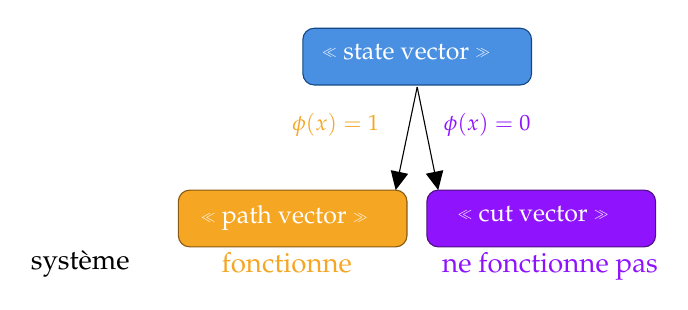
\begin{tikzpicture}[x=0.75pt,y=0.75pt,yscale=-1,xscale=1]
%uncomment if require: \path (0,300); %set diagram left start at 0, and has height of 300

%Rounded Rect [id:dp26160248048613566] 
\draw  [color={rgb, 255:red, 18; green, 72; blue, 135 }  ,draw opacity=1 ][fill={rgb, 255:red, 74; green, 144; blue, 226 }  ,fill opacity=1 ] (139.33,25.8) .. controls (139.33,22.78) and (141.77,20.33) .. (144.79,20.33) -- (244.03,20.33) .. controls (247.04,20.33) and (249.49,22.78) .. (249.49,25.8) -- (249.49,42.2) .. controls (249.49,45.22) and (247.04,47.67) .. (244.03,47.67) -- (144.79,47.67) .. controls (141.77,47.67) and (139.33,45.22) .. (139.33,42.2) -- cycle ;

%Rounded Rect [id:dp2721991232596781] 
\draw  [color={rgb, 255:red, 135; green, 91; blue, 19 }  ,draw opacity=1 ][fill={rgb, 255:red, 245; green, 166; blue, 35 }  ,fill opacity=1 ] (79.33,103.8) .. controls (79.33,100.78) and (81.77,98.33) .. (84.79,98.33) -- (184.03,98.33) .. controls (187.04,98.33) and (189.49,100.78) .. (189.49,103.8) -- (189.49,120.2) .. controls (189.49,123.22) and (187.04,125.67) .. (184.03,125.67) -- (84.79,125.67) .. controls (81.77,125.67) and (79.33,123.22) .. (79.33,120.2) -- cycle ;

%Rounded Rect [id:dp5388212851958989] 
\draw  [color={rgb, 255:red, 76; green, 16; blue, 128 }  ,draw opacity=1 ][fill={rgb, 255:red, 144; green, 19; blue, 254 }  ,fill opacity=1 ] (199.08,103.8) .. controls (199.08,100.78) and (201.53,98.33) .. (204.55,98.33) -- (303.78,98.33) .. controls (306.8,98.33) and (309.25,100.78) .. (309.25,103.8) -- (309.25,120.2) .. controls (309.25,123.22) and (306.8,125.67) .. (303.78,125.67) -- (204.55,125.67) .. controls (201.53,125.67) and (199.08,123.22) .. (199.08,120.2) -- cycle ;

%Straight Lines [id:da8790339481399667] 
\draw    (194.41,48.67) -- (184.64,95.4) ;
\draw [shift={(184.03,98.33)}, rotate = 281.81] [fill={rgb, 255:red, 0; green, 0; blue, 0 }  ][line width=0.08]  [draw opacity=0] (8.93,-4.29) -- (0,0) -- (8.93,4.29) -- cycle    ;
%Straight Lines [id:da5443992444630641] 
\draw    (194.41,48.67) -- (203.95,95.39) ;
\draw [shift={(204.55,98.33)}, rotate = 258.46] [fill={rgb, 255:red, 0; green, 0; blue, 0 }  ][line width=0.08]  [draw opacity=0] (8.93,-4.29) -- (0,0) -- (8.93,4.29) -- cycle    ;

% Text Node
\draw (147.41,26.5) node [anchor=north west][inner sep=0.75pt]  [font=\small,color={rgb, 255:red, 255; green, 255; blue, 255 }  ,opacity=1 ] [align=left] {« state vector »};
% Text Node
\draw (88.91,104.5) node [anchor=north west][inner sep=0.75pt]  [font=\small,color={rgb, 255:red, 255; green, 255; blue, 255 }  ,opacity=1 ] [align=left] {« path vector »};
% Text Node
\draw (212.66,104.5) node [anchor=north west][inner sep=0.75pt]  [font=\small,color={rgb, 255:red, 255; green, 255; blue, 255 }  ,opacity=1 ] [align=left] {« cut vector »};
% Text Node
\draw (7,126) node [anchor=north west][inner sep=0.75pt]   [align=left] {système};
% Text Node
\draw (98.91,127) node [anchor=north west][inner sep=0.75pt]   [align=left] {\textcolor[rgb]{0.96,0.65,0.14}{fonctionne}};
% Text Node
\draw (205.16,127) node [anchor=north west][inner sep=0.75pt]   [align=left] {\textcolor[rgb]{0.56,0.07,1}{ne fonctionne pas}};
% Text Node
\draw (133,60) node [anchor=north west][inner sep=0.75pt]   [align=left] {{\footnotesize \textcolor[rgb]{0.96,0.65,0.14}{$\displaystyle \phi ( x) =1$}}};
% Text Node
\draw (206,60) node [anchor=north west][inner sep=0.75pt]   [align=left] {{\footnotesize $\displaystyle \textcolor[rgb]{0.56,0.07,1}{\phi ( x) =0}$}};
\end{tikzpicture}
\end{center}


\subsubsection{Systèmes communs}
\begin{definitionNOHFILL}[Système parallèle]
Fonctionne tant qu'au moins une des composantes du système fonctionne.
\begin{center}
\tikzset{every picture/.style={line width=0.75pt}} %set default line width to 0.75pt        
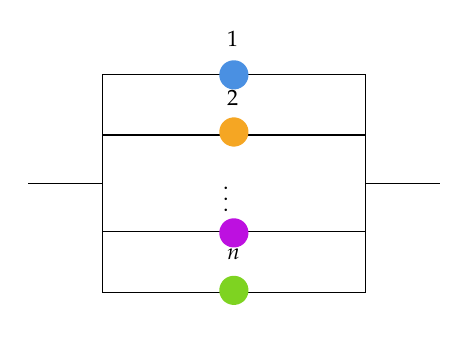
\begin{tikzpicture}[x=0.75pt,y=0.75pt,yscale=-1,xscale=1]
%uncomment if require: \path (0,181); %set diagram left start at 0, and has height of 181

%Shape: Resistor [id:dp9041851120502824] 
\draw   (135.67,43) -- (262.5,43) -- (262.5,148) -- (135.67,148) -- (135.67,43) -- cycle (100,95.5) -- (135.67,95.5) (262.5,95.5) -- (298.17,95.5) ;
%Shape: Rectangle [id:dp7404277637291381] 
\draw   (135.67,72) -- (262.5,72) -- (262.5,118.67) -- (135.67,118.67) -- cycle ;
%Flowchart: Connector [id:dp5328715828334836] 
\draw  [draw opacity=0][fill={rgb, 255:red, 189; green, 16; blue, 224 }  ,fill opacity=1 ][line width=3]  (194.64,124.62) .. controls (191.63,122.16) and (191.18,117.73) .. (193.63,114.72) .. controls (196.09,111.71) and (200.52,111.26) .. (203.53,113.72) .. controls (206.54,116.17) and (206.99,120.6) .. (204.53,123.61) .. controls (202.08,126.62) and (197.65,127.07) .. (194.64,124.62) -- cycle ;
%Flowchart: Connector [id:dp7204615964492069] 
\draw  [draw opacity=0][fill={rgb, 255:red, 74; green, 144; blue, 226 }  ,fill opacity=1 ][line width=3]  (194.64,48.48) .. controls (191.63,46.03) and (191.18,41.6) .. (193.63,38.59) .. controls (196.09,35.58) and (200.52,35.13) .. (203.53,37.58) .. controls (206.54,40.04) and (206.99,44.46) .. (204.53,47.47) .. controls (202.08,50.48) and (197.65,50.93) .. (194.64,48.48) -- cycle ;
%Flowchart: Connector [id:dp3810241352299426] 
\draw  [draw opacity=0][fill={rgb, 255:red, 126; green, 211; blue, 33 }  ,fill opacity=1 ][line width=3]  (194.64,152.31) .. controls (191.63,149.86) and (191.18,145.43) .. (193.63,142.42) .. controls (196.09,139.41) and (200.52,138.96) .. (203.53,141.41) .. controls (206.54,143.87) and (206.99,148.29) .. (204.53,151.3) .. controls (202.08,154.31) and (197.65,154.76) .. (194.64,152.31) -- cycle ;
%Flowchart: Connector [id:dp2801918528278706] 
\draw  [draw opacity=0][fill={rgb, 255:red, 245; green, 166; blue, 35 }  ,fill opacity=1 ][line width=3]  (194.64,76.01) .. controls (191.63,73.55) and (191.18,69.12) .. (193.63,66.11) .. controls (196.09,63.11) and (200.52,62.65) .. (203.53,65.11) .. controls (206.54,67.56) and (206.99,71.99) .. (204.53,75) .. controls (202.08,78.01) and (197.65,78.46) .. (194.64,76.01) -- cycle ;


% Text Node
\draw (194.58,125.81) node [anchor=north west][inner sep=0.75pt]   [align=left] {{\footnotesize $\displaystyle n$}};
% Text Node
\draw (194.58,49.48) node [anchor=north west][inner sep=0.75pt]   [align=left] {{\footnotesize $\displaystyle 2$}};
% Text Node
\draw (194.58,20.57) node [anchor=north west][inner sep=0.75pt]   [align=left] {{\footnotesize $\displaystyle 1$}};
% Text Node
\draw (192.58,87.81) node [anchor=north west][inner sep=0.75pt]   [align=left] {{\footnotesize $\displaystyle \vdots $}};
\end{tikzpicture}
\end{center}
\end{definitionNOHFILL}

\begin{definitionNOHFILL}[Système de série]
Fonctionne seulement si toutes les composantes du système fonctionnent.
\begin{center}
\tikzset{every picture/.style={line width=0.75pt}} %set default line width to 0.75pt        
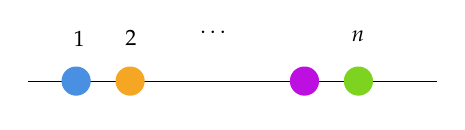
\begin{tikzpicture}[x=0.75pt,y=0.75pt,yscale=-1,xscale=1]
%uncomment if require: \path (0,75); %set diagram left start at 0, and has height of 75

%Straight Lines [id:da021488622482164876] 
\draw    (98,41) -- (294.83,41) ;
%Flowchart: Connector [id:dp05796532763815576] 
\draw  [draw opacity=0][fill={rgb, 255:red, 189; green, 16; blue, 224 }  ,fill opacity=1 ][line width=3]  (226.64,46.45) .. controls (223.63,44) and (223.18,39.57) .. (225.63,36.56) .. controls (228.09,33.55) and (232.52,33.1) .. (235.53,35.55) .. controls (238.54,38.01) and (238.99,42.44) .. (236.53,45.45) .. controls (234.08,48.45) and (229.65,48.91) .. (226.64,46.45) -- cycle ;
%Flowchart: Connector [id:dp06089365703547989] 
\draw  [draw opacity=0][fill={rgb, 255:red, 74; green, 144; blue, 226 }  ,fill opacity=1 ][line width=3]  (116.64,46.45) .. controls (113.63,44) and (113.18,39.57) .. (115.63,36.56) .. controls (118.09,33.55) and (122.52,33.1) .. (125.53,35.55) .. controls (128.54,38.01) and (128.99,42.44) .. (126.53,45.45) .. controls (124.08,48.45) and (119.65,48.91) .. (116.64,46.45) -- cycle ;
%Flowchart: Connector [id:dp2598526793406035] 
\draw  [draw opacity=0][fill={rgb, 255:red, 126; green, 211; blue, 33 }  ,fill opacity=1 ][line width=3]  (252.64,46.45) .. controls (249.63,44) and (249.18,39.57) .. (251.63,36.56) .. controls (254.09,33.55) and (258.52,33.1) .. (261.53,35.55) .. controls (264.54,38.01) and (264.99,42.44) .. (262.53,45.45) .. controls (260.08,48.45) and (255.65,48.91) .. (252.64,46.45) -- cycle ;
%Flowchart: Connector [id:dp554938168736538] 
\draw  [draw opacity=0][fill={rgb, 255:red, 245; green, 166; blue, 35 }  ,fill opacity=1 ][line width=3]  (142.64,46.45) .. controls (139.63,44) and (139.18,39.57) .. (141.63,36.56) .. controls (144.09,33.55) and (148.52,33.1) .. (151.53,35.55) .. controls (154.54,38.01) and (154.99,42.44) .. (152.53,45.45) .. controls (150.08,48.45) and (145.65,48.91) .. (142.64,46.45) -- cycle ;


% Text Node
\draw (252.58,15.54) node [anchor=north west][inner sep=0.75pt]   [align=left] {{\footnotesize $\displaystyle n$}};
% Text Node
\draw (143.58,15.54) node [anchor=north west][inner sep=0.75pt]   [align=left] {{\footnotesize $\displaystyle 2$}};
% Text Node
\draw (118.58,15.54) node [anchor=north west][inner sep=0.75pt]   [align=left] {{\footnotesize $\displaystyle 1$}};
% Text Node
\draw (179.58,15.54) node [anchor=north west][inner sep=0.75pt]   [align=left] {{\footnotesize $\displaystyle \dotsc $}};
\end{tikzpicture}
\end{center}
\end{definitionNOHFILL}

\begin{definitionNOHFILL}[Système de $k$ parmi $n$]
Fonction si au moins $k$ des $n$ composantes du système fonctionnent.\\

\begin{center}
\tikzset{every picture/.style={line width=0.75pt}} %set default line width to 0.75pt        
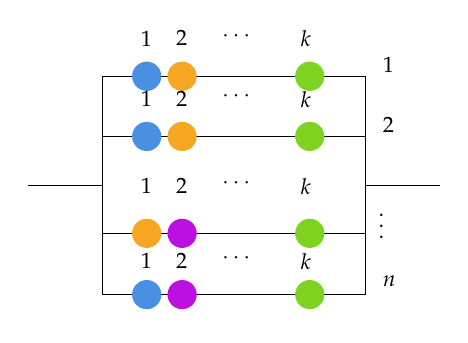
\begin{tikzpicture}[x=0.75pt,y=0.75pt,yscale=-1,xscale=1]
%uncomment if require: \path (0,181); %set diagram left start at 0, and has height of 181
%Shape: Resistor [id:dp02084213653192868] 
\draw   (135.67,43) -- (262.5,43) -- (262.5,148) -- (135.67,148) -- (135.67,43) -- cycle (100,95.5) -- (135.67,95.5) (262.5,95.5) -- (298.17,95.5) ;
%Shape: Rectangle [id:dp11081934562945683] 
\draw   (135.67,72) -- (262.5,72) -- (262.5,118.67) -- (135.67,118.67) -- cycle ;
%Flowchart: Connector [id:dp9558303902983338] 
\draw  [draw opacity=0][fill={rgb, 255:red, 189; green, 16; blue, 224 }  ,fill opacity=1 ][line width=3]  (169.7,124.08) .. controls (166.69,121.62) and (166.24,117.2) .. (168.69,114.19) .. controls (171.14,111.18) and (175.57,110.73) .. (178.58,113.18) .. controls (181.59,115.63) and (182.04,120.06) .. (179.59,123.07) .. controls (177.14,126.08) and (172.71,126.53) .. (169.7,124.08) -- cycle ;
%Flowchart: Connector [id:dp9674121226101444] 
\draw  [draw opacity=0][fill={rgb, 255:red, 126; green, 211; blue, 33 }  ,fill opacity=1 ][line width=3]  (231.2,124.08) .. controls (228.19,121.62) and (227.74,117.2) .. (230.19,114.19) .. controls (232.64,111.18) and (237.07,110.73) .. (240.08,113.18) .. controls (243.09,115.63) and (243.54,120.06) .. (241.09,123.07) .. controls (238.64,126.08) and (234.21,126.53) .. (231.2,124.08) -- cycle ;
%Flowchart: Connector [id:dp49020737335221654] 
\draw  [draw opacity=0][fill={rgb, 255:red, 245; green, 166; blue, 35 }  ,fill opacity=1 ][line width=3]  (152.64,124.08) .. controls (149.63,121.62) and (149.18,117.2) .. (151.63,114.19) .. controls (154.09,111.18) and (158.52,110.73) .. (161.53,113.18) .. controls (164.54,115.63) and (164.99,120.06) .. (162.53,123.07) .. controls (160.08,126.08) and (155.65,126.53) .. (152.64,124.08) -- cycle ;
%Flowchart: Connector [id:dp9346249372112778] 
\draw  [draw opacity=0][fill={rgb, 255:red, 74; green, 144; blue, 226 }  ,fill opacity=1 ][line width=3]  (152.64,48.4) .. controls (149.63,45.94) and (149.18,41.51) .. (151.63,38.5) .. controls (154.09,35.49) and (158.52,35.04) .. (161.53,37.5) .. controls (164.54,39.95) and (164.99,44.38) .. (162.53,47.39) .. controls (160.08,50.4) and (155.65,50.85) .. (152.64,48.4) -- cycle ;
%Flowchart: Connector [id:dp9479134143487338] 
\draw  [draw opacity=0][fill={rgb, 255:red, 126; green, 211; blue, 33 }  ,fill opacity=1 ][line width=3]  (231.2,48.4) .. controls (228.19,45.94) and (227.74,41.51) .. (230.19,38.5) .. controls (232.64,35.49) and (237.07,35.04) .. (240.08,37.5) .. controls (243.09,39.95) and (243.54,44.38) .. (241.09,47.39) .. controls (238.64,50.4) and (234.21,50.85) .. (231.2,48.4) -- cycle ;
%Flowchart: Connector [id:dp5508036096154676] 
\draw  [draw opacity=0][fill={rgb, 255:red, 245; green, 166; blue, 35 }  ,fill opacity=1 ][line width=3]  (169.7,48.4) .. controls (166.69,45.94) and (166.24,41.51) .. (168.69,38.5) .. controls (171.14,35.49) and (175.57,35.04) .. (178.58,37.5) .. controls (181.59,39.95) and (182.04,44.38) .. (179.59,47.39) .. controls (177.14,50.4) and (172.71,50.85) .. (169.7,48.4) -- cycle ;
%Flowchart: Connector [id:dp8024113491002776] 
\draw  [draw opacity=0][fill={rgb, 255:red, 74; green, 144; blue, 226 }  ,fill opacity=1 ][line width=3]  (152.64,77.4) .. controls (149.63,74.94) and (149.18,70.51) .. (151.63,67.5) .. controls (154.09,64.49) and (158.52,64.04) .. (161.53,66.5) .. controls (164.54,68.95) and (164.99,73.38) .. (162.53,76.39) .. controls (160.08,79.4) and (155.65,79.85) .. (152.64,77.4) -- cycle ;
%Flowchart: Connector [id:dp2521939268870461] 
\draw  [draw opacity=0][fill={rgb, 255:red, 126; green, 211; blue, 33 }  ,fill opacity=1 ][line width=3]  (231.2,77.4) .. controls (228.19,74.94) and (227.74,70.51) .. (230.19,67.5) .. controls (232.64,64.49) and (237.07,64.04) .. (240.08,66.5) .. controls (243.09,68.95) and (243.54,73.38) .. (241.09,76.39) .. controls (238.64,79.4) and (234.21,79.85) .. (231.2,77.4) -- cycle ;
%Flowchart: Connector [id:dp504508620481257] 
\draw  [draw opacity=0][fill={rgb, 255:red, 245; green, 166; blue, 35 }  ,fill opacity=1 ][line width=3]  (169.7,77.4) .. controls (166.69,74.94) and (166.24,70.51) .. (168.69,67.5) .. controls (171.14,64.49) and (175.57,64.04) .. (178.58,66.5) .. controls (181.59,68.95) and (182.04,73.38) .. (179.59,76.39) .. controls (177.14,79.4) and (172.71,79.85) .. (169.7,77.4) -- cycle ;
%Flowchart: Connector [id:dp7665075450687393] 
\draw  [draw opacity=0][fill={rgb, 255:red, 74; green, 144; blue, 226 }  ,fill opacity=1 ][line width=3]  (152.64,153.6) .. controls (149.63,151.14) and (149.18,146.71) .. (151.63,143.71) .. controls (154.09,140.7) and (158.52,140.24) .. (161.53,142.7) .. controls (164.54,145.15) and (164.99,149.58) .. (162.53,152.59) .. controls (160.08,155.6) and (155.65,156.05) .. (152.64,153.6) -- cycle ;
%Flowchart: Connector [id:dp30988461089142083] 
\draw  [draw opacity=0][fill={rgb, 255:red, 126; green, 211; blue, 33 }  ,fill opacity=1 ][line width=3]  (231.2,153.6) .. controls (228.19,151.14) and (227.74,146.71) .. (230.19,143.71) .. controls (232.64,140.7) and (237.07,140.24) .. (240.08,142.7) .. controls (243.09,145.15) and (243.54,149.58) .. (241.09,152.59) .. controls (238.64,155.6) and (234.21,156.05) .. (231.2,153.6) -- cycle ;
%Flowchart: Connector [id:dp8751553797176601] 
\draw  [draw opacity=0][fill={rgb, 255:red, 189; green, 16; blue, 224 }  ,fill opacity=1 ][line width=3]  (169.7,153.6) .. controls (166.69,151.14) and (166.24,146.71) .. (168.69,143.71) .. controls (171.14,140.7) and (175.57,140.24) .. (178.58,142.7) .. controls (181.59,145.15) and (182.04,149.58) .. (179.59,152.59) .. controls (177.14,155.6) and (172.71,156.05) .. (169.7,153.6) -- cycle ;

% Text Node
\draw (269.58,137.81) node [anchor=north west][inner sep=0.75pt]   [align=left] {{\footnotesize $\displaystyle n$}};
% Text Node
\draw (269.58,61.48) node [anchor=north west][inner sep=0.75pt]   [align=left] {{\footnotesize $\displaystyle 2$}};
% Text Node
\draw (269.58,32.57) node [anchor=north west][inner sep=0.75pt]   [align=left] {{\footnotesize $\displaystyle 1$}};
% Text Node
\draw (267.58,99.81) node [anchor=north west][inner sep=0.75pt]   [align=left] {{\footnotesize $\displaystyle \vdots $}};
% Text Node
\draw (192.08,126.81) node [anchor=north west][inner sep=0.75pt]   [align=left] {{\footnotesize $\displaystyle \cdots $}};
% Text Node
\draw (153,126.81) node [anchor=north west][inner sep=0.75pt]   [align=left] {{\footnotesize $\displaystyle 1$}};
% Text Node
\draw (170,126.81) node [anchor=north west][inner sep=0.75pt]   [align=left] {{\footnotesize $\displaystyle 2$}};
% Text Node
\draw (230,126.81) node [anchor=north west][inner sep=0.75pt]   [align=left] {{\footnotesize $\displaystyle k$}};
% Text Node
\draw (192.08,90.81) node [anchor=north west][inner sep=0.75pt]   [align=left] {{\footnotesize $\displaystyle \cdots $}};
% Text Node
\draw (153,90.81) node [anchor=north west][inner sep=0.75pt]   [align=left] {{\footnotesize $\displaystyle 1$}};
% Text Node
\draw (170,90.81) node [anchor=north west][inner sep=0.75pt]   [align=left] {{\footnotesize $\displaystyle 2$}};
% Text Node
\draw (230,90.81) node [anchor=north west][inner sep=0.75pt]   [align=left] {{\footnotesize $\displaystyle k$}};
% Text Node
\draw (192.08,19.81) node [anchor=north west][inner sep=0.75pt]   [align=left] {{\footnotesize $\displaystyle \cdots $}};
% Text Node
\draw (153,19.81) node [anchor=north west][inner sep=0.75pt]   [align=left] {{\footnotesize $\displaystyle 1$}};
% Text Node
\draw (170,19.81) node [anchor=north west][inner sep=0.75pt]   [align=left] {{\footnotesize $\displaystyle 2$}};
% Text Node
\draw (230,19.81) node [anchor=north west][inner sep=0.75pt]   [align=left] {{\footnotesize $\displaystyle k$}};
% Text Node
\draw (192.08,48.81) node [anchor=north west][inner sep=0.75pt]   [align=left] {{\footnotesize $\displaystyle \cdots $}};
% Text Node
\draw (153,48.81) node [anchor=north west][inner sep=0.75pt]   [align=left] {{\footnotesize $\displaystyle 1$}};
% Text Node
\draw (170,48.81) node [anchor=north west][inner sep=0.75pt]   [align=left] {{\footnotesize $\displaystyle 2$}};
% Text Node
\draw (230,48.81) node [anchor=north west][inner sep=0.75pt]   [align=left] {{\footnotesize $\displaystyle k$}};
\end{tikzpicture}
\end{center}

\begin{itemize}
	\item	Un système parallèle est donc un système de $1$ parmi $n$ et un système de série un système de $n$ parmi $n$.
\end{itemize}
\end{definitionNOHFILL}

\begin{definitionNOHFILL}[Système de pont]
Il y a deux branches connectées par un pont dans le milieu.
\begin{center}
\tikzset{every picture/.style={line width=0.75pt}} %set default line width to 0.75pt        
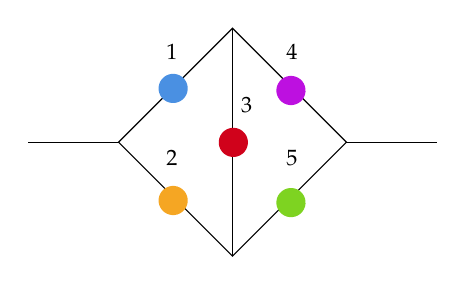
\begin{tikzpicture}[x=0.75pt,y=0.75pt,yscale=-1,xscale=1]
%uncomment if require: \path (0,181); %set diagram left start at 0, and has height of 181

%Shape: Diamond [id:dp8978465211281834] 
\draw   (202.92,31) -- (257.83,85.92) -- (202.92,140.83) -- (148,85.92) -- cycle ;
%Straight Lines [id:da3389217580976256] 
\draw    (104.5,85.92) -- (148,85.92) ;
%Flowchart: Connector [id:dp7317707231673509] 
\draw  [draw opacity=0][fill={rgb, 255:red, 189; green, 16; blue, 224 }  ,fill opacity=1 ][line width=3]  (226.64,66.45) .. controls (223.63,64) and (223.18,59.57) .. (225.63,56.56) .. controls (228.09,53.55) and (232.52,53.1) .. (235.53,55.55) .. controls (238.54,58.01) and (238.99,62.44) .. (236.53,65.45) .. controls (234.08,68.45) and (229.65,68.91) .. (226.64,66.45) -- cycle ;
%Flowchart: Connector [id:dp7843904669196486] 
\draw  [draw opacity=0][fill={rgb, 255:red, 74; green, 144; blue, 226 }  ,fill opacity=1 ][line width=3]  (169.88,65.45) .. controls (166.87,63) and (166.41,58.57) .. (168.87,55.56) .. controls (171.32,52.55) and (175.75,52.1) .. (178.76,54.55) .. controls (181.77,57.01) and (182.22,61.44) .. (179.77,64.45) .. controls (177.31,67.45) and (172.88,67.91) .. (169.88,65.45) -- cycle ;
%Flowchart: Connector [id:dp6258365901565626] 
\draw  [draw opacity=0][fill={rgb, 255:red, 126; green, 211; blue, 33 }  ,fill opacity=1 ][line width=3]  (226.64,120.45) .. controls (223.63,118) and (223.18,113.57) .. (225.63,110.56) .. controls (228.09,107.55) and (232.52,107.1) .. (235.53,109.55) .. controls (238.54,112.01) and (238.99,116.44) .. (236.53,119.45) .. controls (234.08,122.45) and (229.65,122.91) .. (226.64,120.45) -- cycle ;
%Flowchart: Connector [id:dp10191422091926472] 
\draw  [draw opacity=0][fill={rgb, 255:red, 245; green, 166; blue, 35 }  ,fill opacity=1 ][line width=3]  (169.88,119.45) .. controls (166.87,117) and (166.41,112.57) .. (168.87,109.56) .. controls (171.32,106.55) and (175.75,106.1) .. (178.76,108.55) .. controls (181.77,111.01) and (182.22,115.44) .. (179.77,118.45) .. controls (177.31,121.45) and (172.88,121.91) .. (169.88,119.45) -- cycle ;
%Straight Lines [id:da20805937733630953] 
\draw    (202.92,31) -- (202.92,66.33) -- (202.92,140.83) ;
%Straight Lines [id:da7606256354019021] 
\draw    (257.83,85.92) -- (301.33,85.92) ;
%Flowchart: Connector [id:dp6042507902492678] 
\draw  [draw opacity=0][fill={rgb, 255:red, 208; green, 2; blue, 27 }  ,fill opacity=1 ][line width=3]  (198.88,91.45) .. controls (195.87,89) and (195.41,84.57) .. (197.87,81.56) .. controls (200.32,78.55) and (204.75,78.1) .. (207.76,80.55) .. controls (210.77,83.01) and (211.22,87.44) .. (208.77,90.45) .. controls (206.31,93.45) and (201.88,93.91) .. (198.88,91.45) -- cycle ;

% Text Node
\draw (169.82,37.54) node [anchor=north west][inner sep=0.75pt]   [align=left] {{\footnotesize $\displaystyle 1$}};
% Text Node
\draw (169.82,88.54) node [anchor=north west][inner sep=0.75pt]   [align=left] {{\footnotesize $\displaystyle 2$}};
% Text Node
\draw (227.58,88.54) node [anchor=north west][inner sep=0.75pt]   [align=left] {{\footnotesize $\displaystyle 5$}};
% Text Node
\draw (205.82,63.03) node [anchor=north west][inner sep=0.75pt]   [align=left] {{\footnotesize $\displaystyle 3$}};
% Text Node
\draw (227.58,37.54) node [anchor=north west][inner sep=0.75pt]   [align=left] {{\footnotesize $\displaystyle 4$}};
\end{tikzpicture}
\end{center}
\end{definitionNOHFILL}

\textbf{Autres systèmes}	\\
En bref, il y a une infinité de systèmes qui peuvent être construits comme des combinaisons des systèmes précédents.


\columnbreak
\subsection{Minimal path and minimal cut sets}
\begin{definitionNOHFILL}[\og \textit{Path vector} \fg{}]
Vecteur d'états pour lequel le système fonctionne (\lfbox[conditions]{$\phi(\bm{x}) = 1$}). 
\end{definitionNOHFILL}

\begin{definitionNOHFILLsub}[\og \textit{Minimal path vectors} \fg{}]
\og \textit{Path vectors} \fg{} ayant le \textit{minimum} de composantes pour \textbf{fonctionner}. Donc, le système cesse de fonctionner dès qu'une des composantes qui fonctionne échoue. \\

En termes mathématiques, $\bm{x}$ est un \og \textit{minimal path vector} \fg{} si \lfbox[conditions]{$\phi(\bm{y}) = 0 \forall \bm{y} < \bm{x}$}. 
\begin{itemize}
	\item	$\bm{y} < \bm{x}$ implique que tous les éléments $y_{i}$ du vecteur $\bm{y}$ sont inférieurs ou égaux aux éléments $x_{i}$ du vecteur $\bm{x}$ ($y_{i} \leq x_{i} \forall i$) avec au moins un élément qui est strictement inférieur ($y_{i} < x_{i}$ pour au moins un $i$).
\end{itemize}
\end{definitionNOHFILLsub}
 
\begin{definitionNOHFILLsub}[\og \textit{Minimal path sets} \fg{}]
Ensembles minimaux des composantes dont le fonctionnement garanti le fonctionnement du système. Donc, le système fonctionne uniquement si toutes les composantes d'au moins un des \og \textit{minimal path sets} \fg{} fonctionne.
\end{definitionNOHFILLsub}

\begin{formula}{Exemple de système}
\begin{center}
\tikzset{every picture/.style={line width=0.75pt}} %set default line width to 0.75pt        
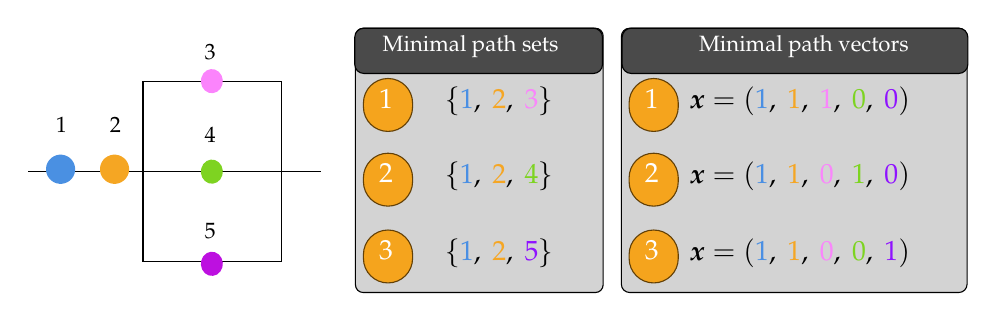
\begin{tikzpicture}[x=0.75pt,y=0.75pt,yscale=-1,xscale=1]
%uncomment if require: \path (0,181); %set diagram left start at 0, and has height of 181

%Shape: Resistor [id:dp10864313661865777] 
\draw   (63.81,51.72) -- (130.69,51.72) -- (130.69,138.61) -- (63.81,138.61) -- (63.81,51.72) -- cycle (45,95.16) -- (63.81,95.16) (130.69,95.16) -- (149.5,95.16) ;
%Straight Lines [id:da8195165620809908] 
\draw    (8.5,95.16) -- (61,95.16) ;
%Flowchart: Connector [id:dp7815712333039893] 
\draw  [draw opacity=0][fill={rgb, 255:red, 74; green, 144; blue, 226 }  ,fill opacity=1 ][line width=3]  (19.64,99.45) .. controls (16.63,97) and (16.18,92.57) .. (18.63,89.56) .. controls (21.09,86.55) and (25.52,86.1) .. (28.53,88.55) .. controls (31.54,91.01) and (31.99,95.44) .. (29.53,98.45) .. controls (27.08,101.45) and (22.65,101.91) .. (19.64,99.45) -- cycle ;
%Flowchart: Connector [id:dp48679332679724796] 
\draw  [draw opacity=0][fill={rgb, 255:red, 245; green, 166; blue, 35 }  ,fill opacity=1 ][line width=3]  (45.64,99.45) .. controls (42.63,97) and (42.18,92.57) .. (44.63,89.56) .. controls (47.09,86.55) and (51.52,86.1) .. (54.53,88.55) .. controls (57.54,91.01) and (57.99,95.44) .. (55.53,98.45) .. controls (53.08,101.45) and (48.65,101.91) .. (45.64,99.45) -- cycle ;
%Flowchart: Connector [id:dp534004442384272] 
\draw  [draw opacity=0][fill={rgb, 255:red, 189; green, 16; blue, 224 }  ,fill opacity=1 ][line width=3]  (93.62,144.08) .. controls (91.36,142.05) and (91.02,138.39) .. (92.87,135.9) .. controls (94.71,133.4) and (98.05,133.03) .. (100.32,135.06) .. controls (102.58,137.09) and (102.92,140.76) .. (101.07,143.25) .. controls (99.23,145.74) and (95.89,146.11) .. (93.62,144.08) -- cycle ;
%Straight Lines [id:da6522970449153964] 
\draw    (63.81,95.16) -- (130.69,95.16) ;
%Flowchart: Connector [id:dp08343329796394117] 
\draw  [draw opacity=0][fill={rgb, 255:red, 251; green, 132; blue, 252 }  ,fill opacity=1 ][line width=3]  (93.62,56.06) .. controls (91.36,54.03) and (91.02,50.37) .. (92.87,47.88) .. controls (94.71,45.39) and (98.05,45.01) .. (100.32,47.04) .. controls (102.58,49.07) and (102.92,52.74) .. (101.07,55.23) .. controls (99.23,57.72) and (95.89,58.09) .. (93.62,56.06) -- cycle ;
%Flowchart: Connector [id:dp8401136867305112] 
\draw  [draw opacity=0][fill={rgb, 255:red, 126; green, 211; blue, 33 }  ,fill opacity=1 ][line width=3]  (93.62,99.67) .. controls (91.36,97.64) and (91.02,93.98) .. (92.87,91.49) .. controls (94.71,89) and (98.05,88.62) .. (100.32,90.65) .. controls (102.58,92.68) and (102.92,96.35) .. (101.07,98.84) .. controls (99.23,101.33) and (95.89,101.7) .. (93.62,99.67) -- cycle ;
%Rounded Rect [id:dp12150470886712084] 
\draw  [color={rgb, 255:red, 0; green, 0; blue, 0 }  ,draw opacity=1 ][fill={rgb, 255:red, 211; green, 211; blue, 211 }  ,fill opacity=1 ] (166.15,29.79) .. controls (166.15,27.73) and (167.82,26.06) .. (169.88,26.06) -- (281.76,26.06) .. controls (283.83,26.06) and (285.5,27.73) .. (285.5,29.79) -- (285.5,149.65) .. controls (285.5,151.72) and (283.83,153.39) .. (281.76,153.39) -- (169.88,153.39) .. controls (167.82,153.39) and (166.15,151.72) .. (166.15,149.65) -- cycle ;
%Rounded Rect [id:dp8405136872936194] 
\draw  [color={rgb, 255:red, 0; green, 0; blue, 0 }  ,draw opacity=1 ][fill={rgb, 255:red, 74; green, 74; blue, 74 }  ,fill opacity=1 ] (165.83,30.41) .. controls (165.83,28.01) and (167.78,26.06) .. (170.19,26.06) -- (280.83,26.06) .. controls (283.24,26.06) and (285.19,28.01) .. (285.19,30.41) -- (285.19,43.49) .. controls (285.19,45.89) and (283.24,47.85) .. (280.83,47.85) -- (170.19,47.85) .. controls (167.78,47.85) and (165.83,45.89) .. (165.83,43.49) -- cycle ;
%Rounded Rect [id:dp9949465583720516] 
\draw  [color={rgb, 255:red, 99; green, 64; blue, 6 }  ,draw opacity=1 ][fill={rgb, 255:red, 245; green, 164; blue, 29 }  ,fill opacity=1 ] (170,62.12) .. controls (170,55.59) and (175.3,50.28) .. (181.84,50.28) -- (181.84,50.28) .. controls (188.38,50.28) and (193.68,55.59) .. (193.68,62.12) -- (193.68,63.95) .. controls (193.68,70.48) and (188.38,75.78) .. (181.84,75.78) -- (181.84,75.78) .. controls (175.3,75.78) and (170,70.48) .. (170,63.95) -- cycle ;

%Rounded Rect [id:dp10249488671228879] 
\draw  [color={rgb, 255:red, 99; green, 64; blue, 6 }  ,draw opacity=1 ][fill={rgb, 255:red, 245; green, 164; blue, 29 }  ,fill opacity=1 ] (170,98.12) .. controls (170,91.59) and (175.3,86.28) .. (181.84,86.28) -- (181.84,86.28) .. controls (188.38,86.28) and (193.68,91.59) .. (193.68,98.12) -- (193.68,99.95) .. controls (193.68,106.48) and (188.38,111.78) .. (181.84,111.78) -- (181.84,111.78) .. controls (175.3,111.78) and (170,106.48) .. (170,99.95) -- cycle ;

%Rounded Rect [id:dp034778547419172856] 
\draw  [color={rgb, 255:red, 99; green, 64; blue, 6 }  ,draw opacity=1 ][fill={rgb, 255:red, 245; green, 164; blue, 29 }  ,fill opacity=1 ] (170,135.12) .. controls (170,128.59) and (175.3,123.28) .. (181.84,123.28) -- (181.84,123.28) .. controls (188.38,123.28) and (193.68,128.59) .. (193.68,135.12) -- (193.68,136.95) .. controls (193.68,143.48) and (188.38,148.78) .. (181.84,148.78) -- (181.84,148.78) .. controls (175.3,148.78) and (170,143.48) .. (170,136.95) -- cycle ;


%Rounded Rect [id:dp02458713610533181] 
\draw  [color={rgb, 255:red, 0; green, 0; blue, 0 }  ,draw opacity=1 ][fill={rgb, 255:red, 211; green, 211; blue, 211 }  ,fill opacity=1 ] (294.27,30.04) .. controls (294.27,27.84) and (296.05,26.06) .. (298.26,26.06) -- (456.85,26.06) .. controls (459.05,26.06) and (460.83,27.84) .. (460.83,30.04) -- (460.83,149.4) .. controls (460.83,151.61) and (459.05,153.39) .. (456.85,153.39) -- (298.26,153.39) .. controls (296.05,153.39) and (294.27,151.61) .. (294.27,149.4) -- cycle ;
%Rounded Rect [id:dp5133060255396584] 
\draw  [color={rgb, 255:red, 0; green, 0; blue, 0 }  ,draw opacity=1 ][fill={rgb, 255:red, 74; green, 74; blue, 74 }  ,fill opacity=1 ] (294.64,30.41) .. controls (294.64,28.01) and (296.59,26.06) .. (299,26.06) -- (456.85,26.06) .. controls (459.25,26.06) and (461.21,28.01) .. (461.21,30.41) -- (461.21,43.49) .. controls (461.21,45.89) and (459.25,47.85) .. (456.85,47.85) -- (299,47.85) .. controls (296.59,47.85) and (294.64,45.89) .. (294.64,43.49) -- cycle ;
%Rounded Rect [id:dp885748416071696] 
\draw  [color={rgb, 255:red, 99; green, 64; blue, 6 }  ,draw opacity=1 ][fill={rgb, 255:red, 245; green, 164; blue, 29 }  ,fill opacity=1 ] (298,62.12) .. controls (298,55.59) and (303.3,50.28) .. (309.84,50.28) -- (309.84,50.28) .. controls (316.38,50.28) and (321.68,55.59) .. (321.68,62.12) -- (321.68,63.95) .. controls (321.68,70.48) and (316.38,75.78) .. (309.84,75.78) -- (309.84,75.78) .. controls (303.3,75.78) and (298,70.48) .. (298,63.95) -- cycle ;

%Rounded Rect [id:dp017152506202217532] 
\draw  [color={rgb, 255:red, 99; green, 64; blue, 6 }  ,draw opacity=1 ][fill={rgb, 255:red, 245; green, 164; blue, 29 }  ,fill opacity=1 ] (298,98.12) .. controls (298,91.59) and (303.3,86.28) .. (309.84,86.28) -- (309.84,86.28) .. controls (316.38,86.28) and (321.68,91.59) .. (321.68,98.12) -- (321.68,99.95) .. controls (321.68,106.48) and (316.38,111.78) .. (309.84,111.78) -- (309.84,111.78) .. controls (303.3,111.78) and (298,106.48) .. (298,99.95) -- cycle ;

%Rounded Rect [id:dp7493392420849236] 
\draw  [color={rgb, 255:red, 99; green, 64; blue, 6 }  ,draw opacity=1 ][fill={rgb, 255:red, 245; green, 164; blue, 29 }  ,fill opacity=1 ] (298,135.12) .. controls (298,128.59) and (303.3,123.28) .. (309.84,123.28) -- (309.84,123.28) .. controls (316.38,123.28) and (321.68,128.59) .. (321.68,135.12) -- (321.68,136.95) .. controls (321.68,143.48) and (316.38,148.78) .. (309.84,148.78) -- (309.84,148.78) .. controls (303.3,148.78) and (298,143.48) .. (298,136.95) -- cycle ;

% Text Node
\draw (176.34,54.03) node [anchor=north west][inner sep=0.75pt]  [color={rgb, 255:red, 255; green, 255; blue, 255 }  ,opacity=1 ] [align=left] {\textcolor[rgb]{1,1,1}{$\displaystyle 1$}};
% Text Node
\draw (176.34,90.03) node [anchor=north west][inner sep=0.75pt]  [color={rgb, 255:red, 255; green, 255; blue, 255 }  ,opacity=1 ] [align=left] {\textcolor[rgb]{1,1,1}{$\displaystyle 2$}};
% Text Node
\draw (176.34,127.03) node [anchor=north west][inner sep=0.75pt]  [color={rgb, 255:red, 255; green, 255; blue, 255 }  ,opacity=1 ] [align=left] {\textcolor[rgb]{1,1,1}{$\displaystyle 3$}};
% Text Node
\draw (178.01,28.45) node [anchor=north west][inner sep=0.75pt]  [color={rgb, 255:red, 255; green, 255; blue, 255 }  ,opacity=1 ] [align=left] {{\footnotesize Minimal path sets}};
% Text Node
\draw (208,53.28) node [anchor=north west][inner sep=0.75pt]   [align=left] {$\displaystyle \{\textcolor[rgb]{0.29,0.56,0.89}{1} ,\ \textcolor[rgb]{0.96,0.65,0.14}{2} ,\ \textcolor[rgb]{0.98,0.52,0.99}{3}\}$};
% Text Node
\draw (208,89.28) node [anchor=north west][inner sep=0.75pt]   [align=left] {$\displaystyle \{\textcolor[rgb]{0.29,0.56,0.89}{1} ,\ \textcolor[rgb]{0.96,0.65,0.14}{2} ,\ \textcolor[rgb]{0.49,0.83,0.13}{4}\}$};
% Text Node
\draw (208,126.28) node [anchor=north west][inner sep=0.75pt]   [align=left] {$\displaystyle \{\textcolor[rgb]{0.29,0.56,0.89}{1} ,\ \textcolor[rgb]{0.96,0.65,0.14}{2} ,\ \textcolor[rgb]{0.56,0.07,1}{5}\}$};
% Text Node
\draw (304.34,127.03) node [anchor=north west][inner sep=0.75pt]  [color={rgb, 255:red, 255; green, 255; blue, 255 }  ,opacity=1 ] [align=left] {\textcolor[rgb]{1,1,1}{$\displaystyle 3$}};
% Text Node
\draw (304.34,90.03) node [anchor=north west][inner sep=0.75pt]  [color={rgb, 255:red, 255; green, 255; blue, 255 }  ,opacity=1 ] [align=left] {\textcolor[rgb]{1,1,1}{$\displaystyle 2$}};
% Text Node
\draw (304.34,54.03) node [anchor=north west][inner sep=0.75pt]  [color={rgb, 255:red, 255; green, 255; blue, 255 }  ,opacity=1 ] [align=left] {\textcolor[rgb]{1,1,1}{$\displaystyle 1$}};
% Text Node
\draw (330.42,28.45) node [anchor=north west][inner sep=0.75pt]  [color={rgb, 255:red, 255; green, 255; blue, 255 }  ,opacity=1 ] [align=left] {{\footnotesize Minimal path vectors}};
% Text Node
\draw (326,53.28) node [anchor=north west][inner sep=0.75pt]   [align=left] {$\displaystyle \bm{x}=(\textcolor[rgb]{0.29,0.56,0.89}{1} ,\ \textcolor[rgb]{0.96,0.65,0.14}{1} ,\ \textcolor[rgb]{0.98,0.52,0.99}{1} ,\ \textcolor[rgb]{0.49,0.83,0.13}{0} ,\ \textcolor[rgb]{0.56,0.07,1}{0})$};
% Text Node
\draw (326,89.28) node [anchor=north west][inner sep=0.75pt]   [align=left] {$\displaystyle \bm{x}=(\textcolor[rgb]{0.29,0.56,0.89}{1} ,\ \textcolor[rgb]{0.96,0.65,0.14}{1} ,\ \textcolor[rgb]{0.98,0.52,0.99}{0} ,\ \textcolor[rgb]{0.49,0.83,0.13}{1} ,\ \textcolor[rgb]{0.56,0.07,1}{0})$};
% Text Node
\draw (326,126.28) node [anchor=north west][inner sep=0.75pt]   [align=left] {$\displaystyle \bm{x}=(\textcolor[rgb]{0.29,0.56,0.89}{1} ,\ \textcolor[rgb]{0.96,0.65,0.14}{1} ,\ \textcolor[rgb]{0.98,0.52,0.99}{0} ,\ \textcolor[rgb]{0.49,0.83,0.13}{0} ,\ \textcolor[rgb]{0.56,0.07,1}{1})$};
% Text Node
\draw (20.58,67.54) node [anchor=north west][inner sep=0.75pt]   [align=left] {{\footnotesize $\displaystyle 1$}};
% Text Node
\draw (46.58,67.54) node [anchor=north west][inner sep=0.75pt]   [align=left] {{\footnotesize $\displaystyle 2$}};
% Text Node
\draw (92.22,32.52) node [anchor=north west][inner sep=0.75pt]   [align=left] {{\footnotesize $\displaystyle 3$}};
% Text Node
\draw (92.22,118.78) node [anchor=north west][inner sep=0.75pt]   [align=left] {{\footnotesize $\displaystyle 5$}};
% Text Node
\draw (92.22,72.44) node [anchor=north west][inner sep=0.75pt]   [align=left] {{\footnotesize $\displaystyle 4$}};
\end{tikzpicture}
\end{center}

Pour bien comprendre la condition pour qu'un \og \textit{mimimal path vector} \fg{}, on observe les vecteurs $\bm{y}$ du premier \og \textit{minimal path vector} \fg{} $\bm{x}$ :
\begin{center}
\tikzset{every picture/.style={line width=0.75pt}} %set default line width to 0.75pt        
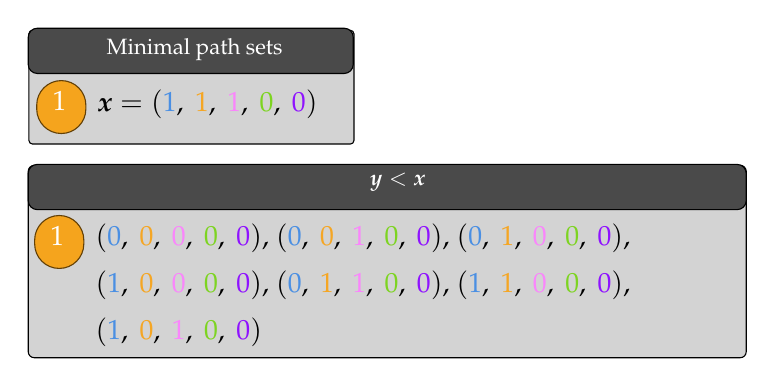
\begin{tikzpicture}[x=0.75pt, y=0.75pt, yscale=-1, xscale=1]
%uncomment if require: \path (0,181); %set diagram left start at 0, and has height of 181

%Rounded Rect [id:dp5716118277000177] 
\draw  [color={rgb, 255:red, 0; green, 0; blue, 0 }  ,draw opacity=1 ][fill={rgb, 255:red, 211; green, 211; blue, 211 }  ,fill opacity=1 ] (6.24,15.25) .. controls (6.24,14.31) and (7.01,13.54) .. (7.96,13.54) -- (161.11,13.54) .. controls (162.06,13.54) and (162.83,14.31) .. (162.83,15.25) -- (162.83,66.62) .. controls (162.83,67.57) and (162.06,68.33) .. (161.11,68.33) -- (7.96,68.33) .. controls (7.01,68.33) and (6.24,67.57) .. (6.24,66.62) -- cycle ;
%Rounded Rect [id:dp5467244252187071] 
\draw  [color={rgb, 255:red, 0; green, 0; blue, 0 }  ,draw opacity=1 ][fill={rgb, 255:red, 74; green, 74; blue, 74 }  ,fill opacity=1 ] (5.9,16.9) .. controls (5.9,14.49) and (7.86,12.54) .. (10.26,12.54) -- (158.13,12.54) .. controls (160.54,12.54) and (162.49,14.49) .. (162.49,16.9) -- (162.49,29.97) .. controls (162.49,32.38) and (160.54,34.33) .. (158.13,34.33) -- (10.26,34.33) .. controls (7.86,34.33) and (5.9,32.38) .. (5.9,29.97) -- cycle ;
%Rounded Rect [id:dp5816118476820735] 
\draw  [color={rgb, 255:red, 99; green, 64; blue, 6 }  ,draw opacity=1 ][fill={rgb, 255:red, 245; green, 164; blue, 29 }  ,fill opacity=1 ] (9.99,49.61) .. controls (9.99,43.07) and (15.29,37.77) .. (21.83,37.77) -- (21.83,37.77) .. controls (28.37,37.77) and (33.67,43.07) .. (33.67,49.61) -- (33.67,51.43) .. controls (33.67,57.97) and (28.37,63.27) .. (21.83,63.27) -- (21.83,63.27) .. controls (15.29,63.27) and (9.99,57.97) .. (9.99,51.43) -- cycle ;


%Rounded Rect [id:dp8326734277415833] 
\draw  [color={rgb, 255:red, 0; green, 0; blue, 0 }  ,draw opacity=1 ][fill={rgb, 255:red, 211; green, 211; blue, 211 }  ,fill opacity=1 ] (5.9,81.5) .. controls (5.9,79.9) and (7.2,78.6) .. (8.81,78.6) -- (348.93,78.6) .. controls (350.53,78.6) and (351.83,79.9) .. (351.83,81.5) -- (351.83,168.38) .. controls (351.83,169.98) and (350.53,171.28) .. (348.93,171.28) -- (8.81,171.28) .. controls (7.2,171.28) and (5.9,169.98) .. (5.9,168.38) -- cycle ;
%Rounded Rect [id:dp9375482206881132] 
\draw  [color={rgb, 255:red, 99; green, 64; blue, 6 }  ,draw opacity=1 ][fill={rgb, 255:red, 245; green, 164; blue, 29 }  ,fill opacity=1 ] (9,114.61) .. controls (9,108.07) and (14.3,102.77) .. (20.84,102.77) -- (20.84,102.77) .. controls (27.38,102.77) and (32.68,108.07) .. (32.68,114.61) -- (32.68,116.43) .. controls (32.68,122.97) and (27.38,128.27) .. (20.84,128.27) -- (20.84,128.27) .. controls (14.3,128.27) and (9,122.97) .. (9,116.43) -- cycle ;

%Rounded Rect [id:dp7232443908778818] 
\draw  [color={rgb, 255:red, 0; green, 0; blue, 0 }  ,draw opacity=1 ][fill={rgb, 255:red, 74; green, 74; blue, 74 }  ,fill opacity=1 ] (5.9,82.5) .. controls (5.9,80.1) and (7.86,78.15) .. (10.26,78.15) -- (347.48,78.15) .. controls (349.88,78.15) and (351.83,80.1) .. (351.83,82.5) -- (351.83,95.58) .. controls (351.83,97.98) and (349.88,99.94) .. (347.48,99.94) -- (10.26,99.94) .. controls (7.86,99.94) and (5.9,97.98) .. (5.9,95.58) -- cycle ;


% Text Node
\draw (16.33,41.52) node [anchor=north west][inner sep=0.75pt]  [color={rgb, 255:red, 255; green, 255; blue, 255 }  ,opacity=1 ] [align=left] {\textcolor[rgb]{1,1,1}{$\displaystyle 1$}};
% Text Node
\draw (15.34,106.52) node [anchor=north west][inner sep=0.75pt]  [color={rgb, 255:red, 255; green, 255; blue, 255 }  ,opacity=1 ] [align=left] {\textcolor[rgb]{1,1,1}{$\displaystyle 1$}};
% Text Node
\draw (37,105.77) node [anchor=north west][inner sep=0.75pt]   [align=left] {$\displaystyle (\textcolor[rgb]{0.29,0.56,0.89}{0} ,\ \textcolor[rgb]{0.96,0.65,0.14}{0} ,\ \textcolor[rgb]{0.98,0.52,0.99}{0} ,\ \textcolor[rgb]{0.49,0.83,0.13}{0} ,\ \textcolor[rgb]{0.56,0.07,1}{0})$, $\displaystyle (\textcolor[rgb]{0.29,0.56,0.89}{0} ,\ \textcolor[rgb]{0.96,0.65,0.14}{0} ,\ \textcolor[rgb]{0.98,0.52,0.99}{1} ,\ \textcolor[rgb]{0.49,0.83,0.13}{0} ,\ \textcolor[rgb]{0.56,0.07,1}{0})$, $\displaystyle (\textcolor[rgb]{0.29,0.56,0.89}{0} ,\ \textcolor[rgb]{0.96,0.65,0.14}{1} ,\ \textcolor[rgb]{0.98,0.52,0.99}{0} ,\ \textcolor[rgb]{0.49,0.83,0.13}{0} ,\ \textcolor[rgb]{0.56,0.07,1}{0})$,};
% Text Node
\draw (169.24,81) node [anchor=north west][inner sep=0.75pt]  [color={rgb, 255:red, 255; green, 255; blue, 255 }  ,opacity=1 ] [align=left] {{\footnotesize $\displaystyle \bm{y} < \bm{x}$}};
% Text Node
\draw (37,128) node [anchor=north west][inner sep=0.75pt]   [align=left] {$\displaystyle (\textcolor[rgb]{0.29,0.56,0.89}{1} ,\ \textcolor[rgb]{0.96,0.65,0.14}{0} ,\ \textcolor[rgb]{0.98,0.52,0.99}{0} ,\ \textcolor[rgb]{0.49,0.83,0.13}{0} ,\ \textcolor[rgb]{0.56,0.07,1}{0})$, $\displaystyle (\textcolor[rgb]{0.29,0.56,0.89}{0} ,\ \textcolor[rgb]{0.96,0.65,0.14}{1} ,\ \textcolor[rgb]{0.98,0.52,0.99}{1} ,\ \textcolor[rgb]{0.49,0.83,0.13}{0} ,\ \textcolor[rgb]{0.56,0.07,1}{0})$, $\displaystyle (\textcolor[rgb]{0.29,0.56,0.89}{1} ,\ \textcolor[rgb]{0.96,0.65,0.14}{1} ,\ \textcolor[rgb]{0.98,0.52,0.99}{0} ,\ \textcolor[rgb]{0.49,0.83,0.13}{0} ,\ \textcolor[rgb]{0.56,0.07,1}{0})$,};
% Text Node
\draw (37,151) node [anchor=north west][inner sep=0.75pt]   [align=left] {$\displaystyle (\textcolor[rgb]{0.29,0.56,0.89}{1} ,\ \textcolor[rgb]{0.96,0.65,0.14}{0} ,\ \textcolor[rgb]{0.98,0.52,0.99}{1} ,\ \textcolor[rgb]{0.49,0.83,0.13}{0} ,\ \textcolor[rgb]{0.56,0.07,1}{0})$};
% Text Node
\draw (42.42,15.93) node [anchor=north west][inner sep=0.75pt]  [color={rgb, 255:red, 255; green, 255; blue, 255 }  ,opacity=1 ] [align=left] {{\footnotesize Minimal path sets}};
% Text Node
\draw (37.99,40.77) node [anchor=north west][inner sep=0.75pt]   [align=left] {$\displaystyle \bm{x}  = (\textcolor[rgb]{0.29,0.56,0.89}{1} ,\ \textcolor[rgb]{0.96,0.65,0.14}{1} ,\ \textcolor[rgb]{0.98,0.52,0.99}{1} ,\ \textcolor[rgb]{0.49,0.83,0.13}{0} ,\ \textcolor[rgb]{0.56,0.07,1}{0})$};
\end{tikzpicture}
\end{center}

On note que $\phi(\bm{y}) = 0$ pour tous les vecteurs ce qui fait de $x$ un \og \textit{minimal path vector} \fg{}.
\end{formula}


\begin{definitionNOHFILL}[\og \textit{Cut vector} \fg{}]
Vecteur d'états pour lequel le système ne fonctionne \textbf{pas} (\lfbox[conditions]{$\phi(\bm{x}) = 0$}). 

\begin{itemize}
	\item	C'est donc l'inverse du \og \textit{path vector} \fg{}.
\end{itemize}
\end{definitionNOHFILL}

\begin{definitionNOHFILLsub}[\og \textit{Minimal cut vectors} \fg{}]
\og \textit{Cut vectors} \fg{} ayant le \textit{maximum} de composantes pour ne \textbf{pas fonctionner}. Donc, le système fonctionne dès qu'une des composantes qui ne fonctionne pas est réparée. \\

En termes mathématiques, $\bm{x}$ est un \og \textit{minimal cut vector} \fg{} si \lfbox[conditions]{$\phi(\bm{y}) = 1 \forall \bm{y} > \bm{x}$}. 
\begin{itemize}
	\item	$\bm{y} > \bm{x}$ implique que tous les éléments $y_{i}$ du vecteur $\bm{y}$ sont supérieurs ou égaux aux éléments $x_{i}$ du vecteur $\bm{x}$ ($y_{i} \geq x_{i} \forall i$) avec au moins un élément qui est strictement supérieur ($y_{i} > x_{i}$ pour au moins un $i$).
\end{itemize}
\end{definitionNOHFILLsub}


\begin{definitionNOHFILLsub}[\og \textit{Minimal cut sets} \fg{}]
Ensembles minimaux des composantes \lfbox[formula]{$\mathcal{C}$} dont l'échec garanti l'échec du système. Donc, le système cesse de fonctionner uniquement si toutes les composantes d'au moins un des \og \textit{minimal cut sets} \fg{} cessent de fonctionner.		\\

En termes mathématiques, un \og \textit{minimal cut set} \fg{} $C$ étant donné un \og \textit{minimal cut vector $\bm{x}$} \fg{} est $\{i: x_{i} = 0\}$.
\end{definitionNOHFILLsub}

\begin{formula}{Exemple \og \textit{minimal cut sets} \fg{}}
On peut visualiser ci-dessous que les \og \textit{minimal cut vectors} \fg{} sont les \og \textit{cut vectors} \fg{} pour lesquels tous les vecteurs $\bm{y}$ fonctionnent ($\psi(\bm{y}) = 1$).
\begin{center}
\tikzset{every picture/.style={line width=0.75pt}} %set default line width to 0.75pt        
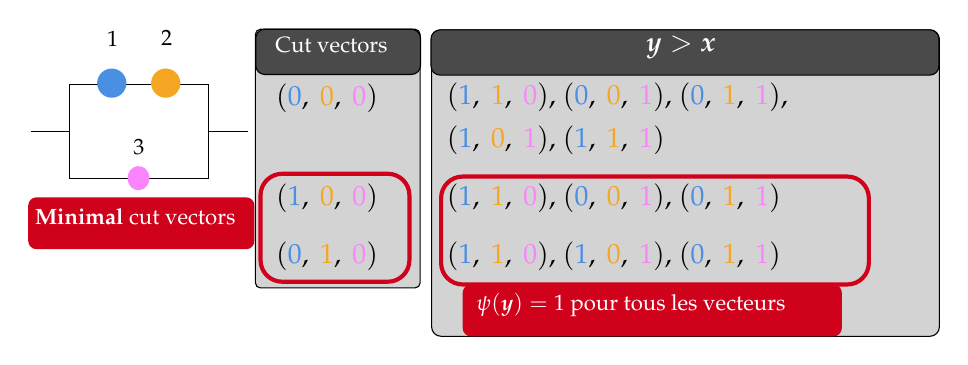
\begin{tikzpicture}[x=0.75pt,y=0.75pt,yscale=-1,xscale=1]
%uncomment if require: \path (0,181); %set diagram left start at 0, and has height of 181
%Shape: Resistor [id:dp16370193622546414] 
\draw   (28.81,45.67) -- (95.69,45.67) -- (95.69,90.83) -- (28.81,90.83) -- (28.81,45.67) -- cycle (10,68.25) -- (28.81,68.25) (95.69,68.25) -- (114.5,68.25) ;

%Flowchart: Connector [id:dp7044092578793344] 
\draw  [draw opacity=0][fill={rgb, 255:red, 251; green, 132; blue, 252 }  ,fill opacity=1 ][line width=3]  (58.62,95.29) .. controls (56.36,93.26) and (56.02,89.59) .. (57.87,87.1) .. controls (59.71,84.61) and (63.05,84.24) .. (65.32,86.27) .. controls (67.58,88.3) and (67.92,91.96) .. (66.07,94.45) .. controls (64.23,96.94) and (60.89,97.32) .. (58.62,95.29) -- cycle ;
%Flowchart: Connector [id:dp8624899692078893] 
\draw  [draw opacity=0][fill={rgb, 255:red, 74; green, 144; blue, 226 }  ,fill opacity=1 ][line width=3]  (44.64,50.45) .. controls (41.63,48) and (41.18,43.57) .. (43.63,40.56) .. controls (46.09,37.55) and (50.52,37.1) .. (53.53,39.55) .. controls (56.54,42.01) and (56.99,46.44) .. (54.53,49.45) .. controls (52.08,52.45) and (47.65,52.91) .. (44.64,50.45) -- cycle ;
%Flowchart: Connector [id:dp7206038017198402] 
\draw  [draw opacity=0][fill={rgb, 255:red, 245; green, 166; blue, 35 }  ,fill opacity=1 ][line width=3]  (70.64,50.45) .. controls (67.63,48) and (67.18,43.57) .. (69.63,40.56) .. controls (72.09,37.55) and (76.52,37.1) .. (79.53,39.55) .. controls (82.54,42.01) and (82.99,46.44) .. (80.53,49.45) .. controls (78.08,52.45) and (73.65,52.91) .. (70.64,50.45) -- cycle ;

%Rounded Rect [id:dp6267729648524285] 
\draw  [color={rgb, 255:red, 0; green, 0; blue, 0 }  ,draw opacity=1 ][fill={rgb, 255:red, 211; green, 211; blue, 211 }  ,fill opacity=1 ] (118.27,21.51) .. controls (118.27,20.13) and (119.38,19.02) .. (120.75,19.02) -- (195.17,19.02) .. controls (196.54,19.02) and (197.66,20.13) .. (197.66,21.51) -- (197.66,141.18) .. controls (197.66,142.55) and (196.54,143.67) .. (195.17,143.67) -- (120.75,143.67) .. controls (119.38,143.67) and (118.27,142.55) .. (118.27,141.18) -- cycle ;
%Rounded Rect [id:dp375244866093164] 
\draw  [color={rgb, 255:red, 0; green, 0; blue, 0 }  ,draw opacity=1 ][fill={rgb, 255:red, 74; green, 74; blue, 74 }  ,fill opacity=1 ] (118.45,23.38) .. controls (118.45,20.97) and (120.4,19.02) .. (122.8,19.02) -- (193.48,19.02) .. controls (195.88,19.02) and (197.83,20.97) .. (197.83,23.38) -- (197.83,36.45) .. controls (197.83,38.86) and (195.88,40.81) .. (193.48,40.81) -- (122.8,40.81) .. controls (120.4,40.81) and (118.45,38.86) .. (118.45,36.45) -- cycle ;
%Rounded Rect [id:dp7741076133467044] 
\draw  [color={rgb, 255:red, 0; green, 0; blue, 0 }  ,draw opacity=1 ][fill={rgb, 255:red, 211; green, 211; blue, 211 }  ,fill opacity=1 ] (203.16,23.95) .. controls (203.16,21.39) and (205.23,19.32) .. (207.78,19.32) -- (443.22,19.32) .. controls (445.77,19.32) and (447.84,21.39) .. (447.84,23.95) -- (447.84,162.35) .. controls (447.84,164.9) and (445.77,166.97) .. (443.22,166.97) -- (207.78,166.97) .. controls (205.23,166.97) and (203.16,164.9) .. (203.16,162.35) -- cycle ;
%Rounded Rect [id:dp7710440832846601] 
\draw  [color={rgb, 255:red, 0; green, 0; blue, 0 }  ,draw opacity=1 ][fill={rgb, 255:red, 74; green, 74; blue, 74 }  ,fill opacity=1 ] (202.9,23.68) .. controls (202.9,21.28) and (204.85,19.32) .. (207.25,19.32) -- (443.22,19.32) .. controls (445.63,19.32) and (447.58,21.28) .. (447.58,23.68) -- (447.58,36.76) .. controls (447.58,39.16) and (445.63,41.11) .. (443.22,41.11) -- (207.25,41.11) .. controls (204.85,41.11) and (202.9,39.16) .. (202.9,36.76) -- cycle ;
%Rounded Rect [id:dp19631031210795125] 
\draw  [color={rgb, 255:red, 208; green, 2; blue, 27 }  ,draw opacity=1 ][line width=1.5]  (120.75,99.07) .. controls (120.75,93.32) and (125.41,88.67) .. (131.15,88.67) -- (182.1,88.67) .. controls (187.84,88.67) and (192.5,93.32) .. (192.5,99.07) -- (192.5,130.27) .. controls (192.5,136.01) and (187.84,140.67) .. (182.1,140.67) -- (131.15,140.67) .. controls (125.41,140.67) and (120.75,136.01) .. (120.75,130.27) -- cycle ;
%Rounded Rect [id:dp9386222478492721] 
\draw  [color={rgb, 255:red, 208; green, 2; blue, 27 }  ,draw opacity=1 ][line width=1.5]  (207.75,100.4) .. controls (207.75,94.66) and (212.41,90) .. (218.15,90) -- (403.43,90) .. controls (409.18,90) and (413.83,94.66) .. (413.83,100.4) -- (413.83,131.6) .. controls (413.83,137.34) and (409.18,142) .. (403.43,142) -- (218.15,142) .. controls (212.41,142) and (207.75,137.34) .. (207.75,131.6) -- cycle ;
%Shape: Rectangle [id:dp10758228081337595] 
\draw  [draw opacity=0][fill={rgb, 255:red, 208; green, 2; blue, 27 }  ,fill opacity=1 ] (8.83,104) .. controls (8.83,101.79) and (10.62,100) .. (12.83,100) -- (113.83,100) .. controls (116.04,100) and (117.83,101.79) .. (117.83,104) -- (117.83,121) .. controls (117.83,123.21) and (116.04,125) .. (113.83,125) -- (12.83,125) .. controls (10.62,125) and (8.83,123.21) .. (8.83,121) -- cycle ;
%Shape: Rectangle [id:dp29322852370945096] 
\draw  [draw opacity=0][fill={rgb, 255:red, 208; green, 2; blue, 27 }  ,fill opacity=1 ] (218.15,146) .. controls (218.15,143.79) and (219.95,142) .. (222.15,142) -- (396.83,142) .. controls (399.04,142) and (400.83,143.79) .. (400.83,146) -- (400.83,163) .. controls (400.83,165.21) and (399.04,167) .. (396.83,167) -- (222.15,167) .. controls (219.95,167) and (218.15,165.21) .. (218.15,163) -- cycle ;

% Text Node
\draw (10.83,104) node [anchor=north west][inner sep=0.75pt]  [color={rgb, 255:red, 0; green, 0; blue, 0 }  ,opacity=1 ] [align=left] {{\footnotesize \textcolor[rgb]{1,1,1}{\textbf{Minimal} cut vectors}}};
% Text Node
\draw (126.96,92.25) node [anchor=north west][inner sep=0.75pt]   [align=left] {$\displaystyle (\textcolor[rgb]{0.29,0.56,0.89}{1} ,\ \textcolor[rgb]{0.96,0.65,0.14}{0} ,\ \textcolor[rgb]{0.98,0.52,0.99}{0})$};
% Text Node
\draw (126.96,44.25) node [anchor=north west][inner sep=0.75pt]   [align=left] {$\displaystyle (\textcolor[rgb]{0.29,0.56,0.89}{0} ,\ \textcolor[rgb]{0.96,0.65,0.14}{0} ,\ \textcolor[rgb]{0.98,0.52,0.99}{0})$};
% Text Node
\draw (126.64,21.42) node [anchor=north west][inner sep=0.75pt]  [color={rgb, 255:red, 255; green, 255; blue, 255 }  ,opacity=1 ] [align=left] {{\footnotesize Cut vectors}};
% Text Node
\draw (126.96,120.25) node [anchor=north west][inner sep=0.75pt]   [align=left] {$\displaystyle (\textcolor[rgb]{0.29,0.56,0.89}{0} ,\ \textcolor[rgb]{0.96,0.65,0.14}{1} ,\ \textcolor[rgb]{0.98,0.52,0.99}{0})$};
% Text Node
\draw (209.25,92.25) node [anchor=north west][inner sep=0.75pt]   [align=left] {$\displaystyle (\textcolor[rgb]{0.29,0.56,0.89}{1} ,\ \textcolor[rgb]{0.96,0.65,0.14}{1} ,\ \textcolor[rgb]{0.98,0.52,0.99}{0})$, $\displaystyle (\textcolor[rgb]{0.29,0.56,0.89}{0} ,\ \textcolor[rgb]{0.96,0.65,0.14}{0} ,\ \textcolor[rgb]{0.98,0.52,0.99}{1})$, $\displaystyle (\textcolor[rgb]{0.29,0.56,0.89}{0} ,\ \textcolor[rgb]{0.96,0.65,0.14}{1} ,\ \textcolor[rgb]{0.98,0.52,0.99}{1})$};
% Text Node
\draw (209.25,43.81) node [anchor=north west][inner sep=0.75pt]   [align=left] {$\displaystyle (\textcolor[rgb]{0.29,0.56,0.89}{1} ,\ \textcolor[rgb]{0.96,0.65,0.14}{1} ,\ \textcolor[rgb]{0.98,0.52,0.99}{0})$, $\displaystyle (\textcolor[rgb]{0.29,0.56,0.89}{0} ,\ \textcolor[rgb]{0.96,0.65,0.14}{0} ,\ \textcolor[rgb]{0.98,0.52,0.99}{1})$, $\displaystyle (\textcolor[rgb]{0.29,0.56,0.89}{0} ,\ \textcolor[rgb]{0.96,0.65,0.14}{1} ,\ \textcolor[rgb]{0.98,0.52,0.99}{1})$,};
% Text Node
\draw (305.24,21.22) node [anchor=north west][inner sep=0.75pt]  [color={rgb, 255:red, 255; green, 255; blue, 255 }  ,opacity=1 ] [align=left] {$\displaystyle \bm{y} > \bm{x}$};
% Text Node
\draw (209.25,120.25) node [anchor=north west][inner sep=0.75pt]   [align=left] {$\displaystyle (\textcolor[rgb]{0.29,0.56,0.89}{1} ,\ \textcolor[rgb]{0.96,0.65,0.14}{1} ,\ \textcolor[rgb]{0.98,0.52,0.99}{0})$, $\displaystyle (\textcolor[rgb]{0.29,0.56,0.89}{1} ,\ \textcolor[rgb]{0.96,0.65,0.14}{0} ,\ \textcolor[rgb]{0.98,0.52,0.99}{1})$, $\displaystyle (\textcolor[rgb]{0.29,0.56,0.89}{0} ,\ \textcolor[rgb]{0.96,0.65,0.14}{1} ,\ \textcolor[rgb]{0.98,0.52,0.99}{1})$};
% Text Node
\draw (209.25,64.11) node [anchor=north west][inner sep=0.75pt]   [align=left] {$\displaystyle (\textcolor[rgb]{0.29,0.56,0.89}{1} ,\ \textcolor[rgb]{0.96,0.65,0.14}{0} ,\ \textcolor[rgb]{0.98,0.52,0.99}{1})$, $\displaystyle (\textcolor[rgb]{0.29,0.56,0.89}{1} ,\ \textcolor[rgb]{0.96,0.65,0.14}{1} ,\ \textcolor[rgb]{0.98,0.52,0.99}{1})$};
% Text Node
\draw (223.49,145) node [anchor=north west][inner sep=0.75pt]  [color={rgb, 255:red, 0; green, 0; blue, 0 }  ,opacity=1 ] [align=left] {{\footnotesize \textcolor[rgb]{1,1,1}{$\displaystyle \psi (\bm{y}) = 1$ pour tous les vecteurs}}};
% Text Node
\draw (58.22,70.75) node [anchor=north west][inner sep=0.75pt]   [align=left] {{\footnotesize $\displaystyle 3$}};
% Text Node
\draw (45.58,18.54) node [anchor=north west][inner sep=0.75pt]   [align=left] {{\footnotesize $\displaystyle 1$}};
% Text Node
\draw (71.58,18.54) node [anchor=north west][inner sep=0.75pt]   [align=left] {{\footnotesize $\displaystyle 2$}};


\end{tikzpicture}
\end{center}
\end{formula}


\begin{center}
\begin{tabular}{|	>{\columncolor{beaublue}}c	|	>{\columncolor{beaublue}}c	|	>{\columncolor{beaublue}}c	|}
\hline\rowcolor{airforceblue} 
 & \multicolumn{2}{c|}{\textcolor{white}{\textbf{Nombre de}}} \\ 
\hline\rowcolor{airforceblue} 
\textcolor{white}{\textbf{Système}} & \textcolor{white}{\textbf{« miminal path sets »}}  & \textcolor{white}{\textbf{« miminal cut sets »}}  \\\specialrule{0.1em}{0em}{0em} 
\hline 
Parallèle & $n$ & $1$ \\ 
\hline 
Série & $1$ & $n$ \\ 
\hline 
$k$ parmi $n$ & $\binom{n}{k}$ & $\binom{n}{n - k + 1}$ \\ 
\hline 
Pont & $4$ & $4$ \\ 
\hline 
\end{tabular} 
\end{center}

Pour un système composé de plusieurs systèmes, le nombre de vecteurs dépend de comment qu'il est organisé.
\begin{center}
\begin{tabular}{| >{\columncolor{beaublue}}c | >{\columncolor{beaublue}}c  | >{\columncolor{beaublue}}c  |}
\hline\rowcolor{airforceblue} 
\textcolor{white}{\textbf{Nombre de}}	&	\textcolor{white}{\textbf{Organisation du système}}	&	\textcolor{white}{\textbf{Action}}		\\\specialrule{0.1em}{0em}{0em} 
	&	parallèle	&	somme	\\\cline{2-3}
\multirow{-2}{*}{\og \textit{minimal path sets} \fg{}}	&	série	&	produit	\\\hline
	&	parallèle	&	produit	\\\cline{2-3}
\multirow{-2}{*}{\og \textit{minimal cut sets} \fg{}}	&	série	&	somme	\\\hline
\end{tabular}
\end{center}


\columnbreak
\subsection{Structure Functions}
\begin{distributions}[Notation]
\begin{description}
	\item[$A_{1}, \dots, A_{s}$]	\og \textit{Minimal path sets} \fg{}.
	\item[$C_{1}, \dots, C_{m}$]	\og \textit{Minimal cut sets} \fg{}.
\end{description}
\end{distributions}
La \og \textit{structure function} \fg{} d'un système peut être déduite par deux approches : 
\begin{enumerate}[label	=	\circled{\arabic*}{trueblue}]
	\item	Approche par les \og \textit{minimal path sets} \fg{}.
	\item	Approche par les \og \textit{minimal cut sets} \fg{}.
\end{enumerate}

\

Cela dit, la fonction de base est fonction de la méthode d'organisation du système : 
\begin{definitionGENERAL}{Système en parallèle}[\circled{1}{trueblue}]
Un système en parallèle fonctionne tant qu'au moins une des composantes fonctionne. Alors, tant qu'au moins une des composantes $i$ a un état de $x_{i} = 1$, l'état du système est de $\phi(\bm{x}) = 1$.	\\
\begin{align*}
	\phi(\bm{x})
	&=	\max\{x_{1}, \dots, x_{n}\}		\\
	&=	1 - \prod_{i = 1}^{n} (1 - x_{i})
\end{align*}

\begin{itemize}
	\item	La deuxième formulation découle du fait que les états sont des variables binaires.
\end{itemize}
\end{definitionGENERAL}

\begin{definitionGENERAL}{Système en série}[\circled{2}{trueblue}]
Un système en parallèle fonctionne ssi toutes les composantes fonctionnent. Alors, dès qu'une composante $i$ a un état de $x_{i} = 0$, l'état du système est de $\phi(\bm{x}) = 0$.	\\
\begin{align*}
	\phi(\bm{x})
	&=	\min\{x_{1}, \dots, x_{n}\}	\\
	&=	\prod_{i = 1}^{n} x_{i}
\end{align*}

\begin{itemize}
	\item	La deuxième formulation découle du fait que les états sont des variables binaires.
\end{itemize}
\end{definitionGENERAL}


\subsubsection{Approche par les \og \textit{minimal path sets} \fg{}}
Soit ces deux constats : 
\begin{enumerate}[label	=	\circled{\arabic*}{trueblue}]
	\item	Un système fonctionne ssi toutes les composantes d'au moins un des \og \textit{minimal path sets} \fg{} fonctionnent.
	\item	Un système en parallèle fonctionne ssi au moins une des composantes fonctionnent.
\end{enumerate}

Alors, tout système peut être traité comme le système en parallèle de ses \og \textit{minimal path sets} \fg{} :
\begin{center}
\tikzset{every picture/.style={line width=0.75pt}} %set default line width to 0.75pt        
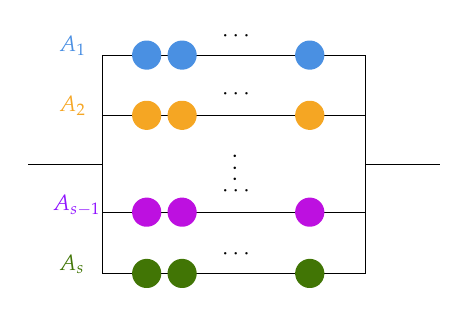
\begin{tikzpicture}[x=0.75pt,y=0.75pt,yscale=-1,xscale=1]
%uncomment if require: \path (0,181); %set diagram left start at 0, and has height of 181

%Shape: Resistor [id:dp8683144921932384] 
\draw   (135.67,43) -- (262.5,43) -- (262.5,148) -- (135.67,148) -- (135.67,43) -- cycle (100,95.5) -- (135.67,95.5) (262.5,95.5) -- (298.17,95.5) ;
%Shape: Rectangle [id:dp49231279059573696] 
\draw   (135.67,72) -- (262.5,72) -- (262.5,118.67) -- (135.67,118.67) -- cycle ;
%Flowchart: Connector [id:dp07800444389002736] 
\draw  [draw opacity=0][fill={rgb, 255:red, 189; green, 16; blue, 224 }  ,fill opacity=1 ][line width=3]  (169.7,124.08) .. controls (166.69,121.62) and (166.24,117.2) .. (168.69,114.19) .. controls (171.14,111.18) and (175.57,110.73) .. (178.58,113.18) .. controls (181.59,115.63) and (182.04,120.06) .. (179.59,123.07) .. controls (177.14,126.08) and (172.71,126.53) .. (169.7,124.08) -- cycle ;
%Flowchart: Connector [id:dp6448168497930598] 
\draw  [draw opacity=0][fill={rgb, 255:red, 189; green, 16; blue, 224 }  ,fill opacity=1 ][line width=3]  (231.2,124.08) .. controls (228.19,121.62) and (227.74,117.2) .. (230.19,114.19) .. controls (232.64,111.18) and (237.07,110.73) .. (240.08,113.18) .. controls (243.09,115.63) and (243.54,120.06) .. (241.09,123.07) .. controls (238.64,126.08) and (234.21,126.53) .. (231.2,124.08) -- cycle ;
%Flowchart: Connector [id:dp030346118463447036] 
\draw  [draw opacity=0][fill={rgb, 255:red, 189; green, 16; blue, 224 }  ,fill opacity=1 ][line width=3]  (152.64,124.08) .. controls (149.63,121.62) and (149.18,117.2) .. (151.63,114.19) .. controls (154.09,111.18) and (158.52,110.73) .. (161.53,113.18) .. controls (164.54,115.63) and (164.99,120.06) .. (162.53,123.07) .. controls (160.08,126.08) and (155.65,126.53) .. (152.64,124.08) -- cycle ;
%Flowchart: Connector [id:dp08541890561200871] 
\draw  [draw opacity=0][fill={rgb, 255:red, 74; green, 144; blue, 226 }  ,fill opacity=1 ][line width=3]  (152.64,48.4) .. controls (149.63,45.94) and (149.18,41.51) .. (151.63,38.5) .. controls (154.09,35.49) and (158.52,35.04) .. (161.53,37.5) .. controls (164.54,39.95) and (164.99,44.38) .. (162.53,47.39) .. controls (160.08,50.4) and (155.65,50.85) .. (152.64,48.4) -- cycle ;
%Flowchart: Connector [id:dp1989646111425234] 
\draw  [draw opacity=0][fill={rgb, 255:red, 74; green, 144; blue, 226 }  ,fill opacity=1 ][line width=3]  (231.2,48.4) .. controls (228.19,45.94) and (227.74,41.51) .. (230.19,38.5) .. controls (232.64,35.49) and (237.07,35.04) .. (240.08,37.5) .. controls (243.09,39.95) and (243.54,44.38) .. (241.09,47.39) .. controls (238.64,50.4) and (234.21,50.85) .. (231.2,48.4) -- cycle ;
%Flowchart: Connector [id:dp35617798386228294] 
\draw  [draw opacity=0][fill={rgb, 255:red, 74; green, 144; blue, 226 }  ,fill opacity=1 ][line width=3]  (169.7,48.4) .. controls (166.69,45.94) and (166.24,41.51) .. (168.69,38.5) .. controls (171.14,35.49) and (175.57,35.04) .. (178.58,37.5) .. controls (181.59,39.95) and (182.04,44.38) .. (179.59,47.39) .. controls (177.14,50.4) and (172.71,50.85) .. (169.7,48.4) -- cycle ;
%Flowchart: Connector [id:dp56251012988241] 
\draw  [draw opacity=0][fill={rgb, 255:red, 245; green, 166; blue, 35 }  ,fill opacity=1 ][line width=3]  (152.64,77.4) .. controls (149.63,74.94) and (149.18,70.51) .. (151.63,67.5) .. controls (154.09,64.49) and (158.52,64.04) .. (161.53,66.5) .. controls (164.54,68.95) and (164.99,73.38) .. (162.53,76.39) .. controls (160.08,79.4) and (155.65,79.85) .. (152.64,77.4) -- cycle ;
%Flowchart: Connector [id:dp9191589506239592] 
\draw  [draw opacity=0][fill={rgb, 255:red, 245; green, 166; blue, 35 }  ,fill opacity=1 ][line width=3]  (231.2,77.4) .. controls (228.19,74.94) and (227.74,70.51) .. (230.19,67.5) .. controls (232.64,64.49) and (237.07,64.04) .. (240.08,66.5) .. controls (243.09,68.95) and (243.54,73.38) .. (241.09,76.39) .. controls (238.64,79.4) and (234.21,79.85) .. (231.2,77.4) -- cycle ;
%Flowchart: Connector [id:dp0674909847030205] 
\draw  [draw opacity=0][fill={rgb, 255:red, 245; green, 166; blue, 35 }  ,fill opacity=1 ][line width=3]  (169.7,77.4) .. controls (166.69,74.94) and (166.24,70.51) .. (168.69,67.5) .. controls (171.14,64.49) and (175.57,64.04) .. (178.58,66.5) .. controls (181.59,68.95) and (182.04,73.38) .. (179.59,76.39) .. controls (177.14,79.4) and (172.71,79.85) .. (169.7,77.4) -- cycle ;
%Flowchart: Connector [id:dp8551077995820422] 
\draw  [draw opacity=0][fill={rgb, 255:red, 65; green, 117; blue, 5 }  ,fill opacity=1 ][line width=3]  (152.64,153.6) .. controls (149.63,151.14) and (149.18,146.71) .. (151.63,143.71) .. controls (154.09,140.7) and (158.52,140.24) .. (161.53,142.7) .. controls (164.54,145.15) and (164.99,149.58) .. (162.53,152.59) .. controls (160.08,155.6) and (155.65,156.05) .. (152.64,153.6) -- cycle ;
%Flowchart: Connector [id:dp9904144062400568] 
\draw  [draw opacity=0][fill={rgb, 255:red, 65; green, 117; blue, 5 }  ,fill opacity=1 ][line width=3]  (231.2,153.6) .. controls (228.19,151.14) and (227.74,146.71) .. (230.19,143.71) .. controls (232.64,140.7) and (237.07,140.24) .. (240.08,142.7) .. controls (243.09,145.15) and (243.54,149.58) .. (241.09,152.59) .. controls (238.64,155.6) and (234.21,156.05) .. (231.2,153.6) -- cycle ;
%Flowchart: Connector [id:dp20218671328806814] 
\draw  [draw opacity=0][fill={rgb, 255:red, 65; green, 117; blue, 5 }  ,fill opacity=1 ][line width=3]  (169.7,153.6) .. controls (166.69,151.14) and (166.24,146.71) .. (168.69,143.71) .. controls (171.14,140.7) and (175.57,140.24) .. (178.58,142.7) .. controls (181.59,145.15) and (182.04,149.58) .. (179.59,152.59) .. controls (177.14,155.6) and (172.71,156.05) .. (169.7,153.6) -- cycle ;

% Text Node
\draw (113.58,137.81) node [anchor=north west][inner sep=0.75pt]   [align=left] {{\footnotesize \textcolor[rgb]{0.25,0.46,0.02}{$\displaystyle A_{s}$}}};
% Text Node
\draw (113.58,61.48) node [anchor=north west][inner sep=0.75pt]   [align=left] {{\footnotesize \textcolor[rgb]{0.96,0.65,0.14}{$\displaystyle A_{2}$}}};
% Text Node
\draw (113.58,32.57) node [anchor=north west][inner sep=0.75pt]   [align=left] {{\footnotesize \textcolor[rgb]{0.29,0.56,0.89}{$\displaystyle A_{1}$}}};
% Text Node
\draw (110.58,109) node [anchor=north west][inner sep=0.75pt]   [align=left] {{\footnotesize \textcolor[rgb]{0.49,0.83,0.13}{$\displaystyle \textcolor[rgb]{0.56,0.07,1}{A_{s-1}}$}}};
% Text Node
\draw (192,30) node [anchor=north west][inner sep=0.75pt]   [align=left] {{\footnotesize $\displaystyle \cdots $}};
% Text Node
\draw (192,58) node [anchor=north west][inner sep=0.75pt]   [align=left] {{\footnotesize $\displaystyle \cdots $}};
% Text Node
\draw (192,105) node [anchor=north west][inner sep=0.75pt]   [align=left] {{\footnotesize $\displaystyle \cdots $}};
% Text Node
\draw (192,135) node [anchor=north west][inner sep=0.75pt]   [align=left] {{\footnotesize $\displaystyle \cdots $}};
% Text Node
\draw (197,82) node [anchor=north west][inner sep=0.75pt]   [align=left] {{\footnotesize $\displaystyle \vdots $}};
\end{tikzpicture}
\end{center}

Il s'ensuit qu'on peut réécrire le système comme : 
\begin{align*}
	\phi(\bm{x})
	&=	\max\left\{\underset{i \in A_{1}}{\min}\ x_{i}, \underset{i \in A_{2}}{\min}\ x_{i}, \dots, \underset{i \in A_{s}}{\min}\ x_{i}\right\}
	=	\underset{j}{\min} \prod_{i \in A_{j}} x_{i}
\end{align*}


\subsubsection{Approche par les \og \textit{minimal cut sets} \fg{}}
Soit ces deux constats : 
\begin{enumerate}[label	=	\circled{\arabic*}{trueblue}]
	\item	Un système cesse de fonctionner ssi toutes les composantes d'au moins un des \og \textit{minimal cut sets} \fg{} cessent de fonctionner.
	\item	Un système en série cesse de fonctionner ssi au moins une des composantes cesse de fonctionner.
\end{enumerate}

Alors, tout système peut être traité comme le système en série de ses \og \textit{minimal cut sets} \fg{} :	
\begin{center}
\tikzset{every picture/.style={line width=0.75pt}} %set default line width to 0.75pt        
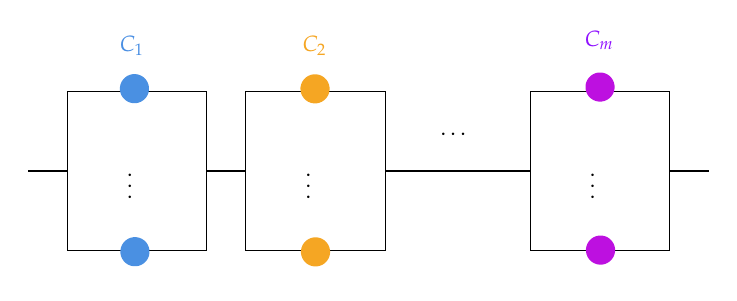
\begin{tikzpicture}[x=0.75pt,y=0.75pt,yscale=-1,xscale=1]
%uncomment if require: \path (0,181); %set diagram left start at 0, and has height of 181

%Shape: Resistor [id:dp031041827587751092] 
\draw   (104.54,46.67) -- (171.63,46.67) -- (171.63,122.89) -- (104.54,122.89) -- (104.54,46.67) -- cycle (85.67,84.78) -- (104.54,84.78) (171.63,84.78) -- (190.5,84.78) ;

%Shape: Resistor [id:dp9977426182626892] 
\draw   (190.54,46.67) -- (257.63,46.67) -- (257.63,122.89) -- (190.54,122.89) -- (190.54,46.67) -- cycle (171.67,84.78) -- (190.54,84.78) (257.63,84.78) -- (276.5,84.78) ;

%Shape: Resistor [id:dp4412566731431071] 
\draw   (327.54,46.67) -- (394.63,46.67) -- (394.63,122.89) -- (327.54,122.89) -- (327.54,46.67) -- cycle (308.67,84.78) -- (327.54,84.78) (394.63,84.78) -- (413.5,84.78) ;

%Flowchart: Connector [id:dp006687567958338025] 
\draw  [draw opacity=0][fill={rgb, 255:red, 189; green, 16; blue, 224 }  ,fill opacity=1 ][line width=3]  (355.93,118.47) .. controls (358.38,115.45) and (362.81,114.99) .. (365.82,117.43) .. controls (368.84,119.88) and (369.3,124.3) .. (366.86,127.32) .. controls (364.41,130.34) and (359.99,130.8) .. (356.97,128.36) .. controls (353.95,125.91) and (353.49,121.48) .. (355.93,118.47) -- cycle ;
%Flowchart: Connector [id:dp3432893660753784] 
\draw  [draw opacity=0][fill={rgb, 255:red, 189; green, 16; blue, 224 }  ,fill opacity=1 ][line width=3]  (355.7,39.91) .. controls (358.15,36.89) and (362.57,36.43) .. (365.59,38.87) .. controls (368.61,41.32) and (369.07,45.75) .. (366.63,48.76) .. controls (364.18,51.78) and (359.75,52.24) .. (356.74,49.8) .. controls (353.72,47.35) and (353.26,42.93) .. (355.7,39.91) -- cycle ;
%Flowchart: Connector [id:dp04374413071027017] 
\draw  [draw opacity=0][fill={rgb, 255:red, 74; green, 144; blue, 226 }  ,fill opacity=1 ][line width=3]  (131.38,40.69) .. controls (133.83,37.67) and (138.26,37.21) .. (141.27,39.65) .. controls (144.29,42.09) and (144.75,46.52) .. (142.31,49.54) .. controls (139.86,52.56) and (135.44,53.02) .. (132.42,50.57) .. controls (129.4,48.13) and (128.94,43.7) .. (131.38,40.69) -- cycle ;
%Flowchart: Connector [id:dp39100303910521084] 
\draw  [draw opacity=0][fill={rgb, 255:red, 74; green, 144; blue, 226 }  ,fill opacity=1 ][line width=3]  (131.62,119.24) .. controls (134.06,116.23) and (138.49,115.76) .. (141.51,118.21) .. controls (144.52,120.65) and (144.99,125.08) .. (142.54,128.1) .. controls (140.1,131.11) and (135.67,131.58) .. (132.65,129.13) .. controls (129.64,126.69) and (129.17,122.26) .. (131.62,119.24) -- cycle ;
%Flowchart: Connector [id:dp5332744563223488] 
\draw  [draw opacity=0][fill={rgb, 255:red, 245; green, 166; blue, 35 }  ,fill opacity=1 ][line width=3]  (218.38,40.77) .. controls (220.83,37.76) and (225.26,37.29) .. (228.27,39.74) .. controls (231.29,42.18) and (231.75,46.61) .. (229.31,49.63) .. controls (226.86,52.64) and (222.44,53.11) .. (219.42,50.66) .. controls (216.4,48.22) and (215.94,43.79) .. (218.38,40.77) -- cycle ;
%Flowchart: Connector [id:dp15304137669616913] 
\draw  [draw opacity=0][fill={rgb, 255:red, 245; green, 166; blue, 35 }  ,fill opacity=1 ][line width=3]  (218.62,119.33) .. controls (221.06,116.31) and (225.49,115.85) .. (228.51,118.29) .. controls (231.52,120.74) and (231.99,125.17) .. (229.54,128.18) .. controls (227.1,131.2) and (222.67,131.66) .. (219.65,129.22) .. controls (216.64,126.77) and (216.17,122.35) .. (218.62,119.33) -- cycle ;
%Straight Lines [id:da4371326826928572] 
\draw    (259.5,84.78) -- (327.54,84.78) ;

% Text Node
\draw (216.58,18.48) node [anchor=north west][inner sep=0.75pt]   [align=left] {{\footnotesize \textcolor[rgb]{0.96,0.65,0.14}{$\displaystyle C_{2}$}}};
% Text Node
\draw (128.58,18.57) node [anchor=north west][inner sep=0.75pt]   [align=left] {{\footnotesize \textcolor[rgb]{0.29,0.56,0.89}{$\displaystyle C_{1}$}}};
% Text Node
\draw (352.58,16) node [anchor=north west][inner sep=0.75pt]   [align=left] {{\footnotesize \textcolor[rgb]{0.49,0.83,0.13}{$\displaystyle \textcolor[rgb]{0.56,0.07,1}{C_{m}}$}}};
% Text Node
\draw (355,77) node [anchor=north west][inner sep=0.75pt]   [align=left] {{\footnotesize $\displaystyle \vdots $}};
% Text Node
\draw (218,77) node [anchor=north west][inner sep=0.75pt]   [align=left] {{\footnotesize $\displaystyle \vdots $}};
% Text Node
\draw (132,77) node [anchor=north west][inner sep=0.75pt]   [align=left] {{\footnotesize $\displaystyle \vdots $}};
% Text Node
\draw (283,65) node [anchor=north west][inner sep=0.75pt]   [align=left] {{\footnotesize $\displaystyle \dotsc $}};
\end{tikzpicture}
\end{center}

Il s'ensuit qu'on peut réécrire le système comme : 
\begin{align*}
	\phi(\bm{x})
	&=	\min\left\{\underset{i \in C_{1}}{\max}\ x_{i}, \underset{i \in C_{2}}{\max}\ x_{i}, \dots, \underset{i \in C_{s}}{\max}\ x_{i}\right\}
	=	\prod_{j = 1}^{m} \max_{i \in C_{j}} x_{i}
\end{align*}

\paragraph{Note}	Puisque l'état est une variable binaire, \lfbox[formula]{$x_{i}^{k} = x_{i}$}.


\columnbreak
\subsection{Fiabilité des systèmes}
\begin{distributions}[Notation]
\begin{description}
	\item[$X_{i}$]	Variable aléatoire suivant une distribution Bernoulli : \lfbox[conditions]{$X_{i} \sim \text{Bernoulli}(p_{i})$}.
		\begin{align*}
		X_{i}
		&=	\begin{cases}
			1,	&	p_{i}	\\
			0,	&	1 - p_{i}
			\end{cases}
		\end{align*}
		\begin{itemize}
		\item	$\bm{X} = (X_{1}, X_{2}, \dots, X_{n})$ vecteur des v.a. Bernoulli.
		\end{itemize}
	\item[$p_{i}$]	Fiabilité de la composante $i$.
		\begin{itemize}
		\item	$\bm{p} = (p_{1}, p_{2}, \dots, p_{n})$ vecteur des fiabilités.
		\end{itemize}
	\item[$r(\bm{p})$]	Fonction de fiabilité du système.
\end{description}
\end{distributions}

\begin{definitionNOHFILL}[Fiabilité]
La fiabilité d'une \textbf{\underline{composante}} est la \textbf{probabilité que la composante fonctionne}.\\

La fiabilité d'un \textbf{\underline{système}} est la \textbf{probabilité que le système fonctionne}.
\end{definitionNOHFILL}

\begin{definitionNOHFILLsub}[Fonction de fiabilité]
Fonction de la fiabilité des composantes \lfbox[formula]{$r(\bm{p})$} qui quantifie la probabilité que le système fonctionne.

\begin{align*}
	r(\bm{p})
	&=	\underbrace{\Pr(\phi(\bm{X}) = 1)}_{\substack{\text{somme des probabilités}\\ \text{des \og \textit{path vectors} \fg{}}}}
	=	1 - \underbrace{\Pr(\phi(\bm{X}) = 0)}_{\substack{\text{somme des probabilités}\\ \text{des \og \textit{cut vectors} \fg{}}}}	\\
	&=	0 \times \Pr(\phi(\bm{X}) = 0) + 1 \times \Pr(\phi(\bm{X}) = 1) 
	= \text{E}[\phi(\bm{X})]
\end{align*}

\begin{itemize}
	\item	Puisque $\phi$ est fonction du vecteur de v.a. Bernoulli $\bm{X}$, $\phi$ est également une v.a. Bernoulli. 
	\item	Il s'ensuit que $r(\bm{p}) = 0 \times \Pr(\phi(\bm{X}) = 0) + 1 \times \Pr(\phi(\bm{X}) = 1) = \text{E}[\phi(\bm{X})]$.
\end{itemize}
\end{definitionNOHFILLsub}

\begin{formula}{Exemple de calcul de la fonction de fiabilité}
\begin{center}
\tikzset{every picture/.style={line width=0.75pt}} %set default line width to 0.75pt        
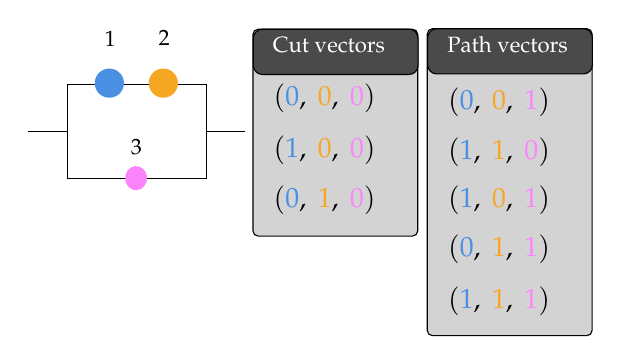
\begin{tikzpicture}[x=0.75pt,y=0.75pt,yscale=-1,xscale=1]
%uncomment if require: \path (0,181); %set diagram left start at 0, and has height of 181

%Rounded Rect [id:dp8878409106243981] 
\draw  [color={rgb, 255:red, 0; green, 0; blue, 0 }  ,draw opacity=1 ][fill={rgb, 255:red, 211; green, 211; blue, 211 }  ,fill opacity=1 ] (118.27,21.51) .. controls (118.27,20.13) and (119.38,19.02) .. (120.75,19.02) -- (195.17,19.02) .. controls (196.54,19.02) and (197.66,20.13) .. (197.66,21.51) -- (197.66,116.18) .. controls (197.66,117.55) and (196.54,118.67) .. (195.17,118.67) -- (120.75,118.67) .. controls (119.38,118.67) and (118.27,117.55) .. (118.27,116.18) -- cycle ;
%Rounded Rect [id:dp5883608057634968] 
\draw  [color={rgb, 255:red, 0; green, 0; blue, 0 }  ,draw opacity=1 ][fill={rgb, 255:red, 74; green, 74; blue, 74 }  ,fill opacity=1 ] (118.45,23.38) .. controls (118.45,20.97) and (120.4,19.02) .. (122.8,19.02) -- (193.48,19.02) .. controls (195.88,19.02) and (197.83,20.97) .. (197.83,23.38) -- (197.83,36.45) .. controls (197.83,38.86) and (195.88,40.81) .. (193.48,40.81) -- (122.8,40.81) .. controls (120.4,40.81) and (118.45,38.86) .. (118.45,36.45) -- cycle ;
%Shape: Resistor [id:dp6289583123756435] 
\draw   (28.81,45.67) -- (95.69,45.67) -- (95.69,90.83) -- (28.81,90.83) -- (28.81,45.67) -- cycle (10,68.25) -- (28.81,68.25) (95.69,68.25) -- (114.5,68.25) ;
%Flowchart: Connector [id:dp7521329945820521] 
\draw  [draw opacity=0][fill={rgb, 255:red, 251; green, 132; blue, 252 }  ,fill opacity=1 ][line width=3]  (58.62,95.29) .. controls (56.36,93.26) and (56.02,89.59) .. (57.87,87.1) .. controls (59.71,84.61) and (63.05,84.24) .. (65.32,86.27) .. controls (67.58,88.3) and (67.92,91.96) .. (66.07,94.45) .. controls (64.23,96.94) and (60.89,97.32) .. (58.62,95.29) -- cycle ;
%Flowchart: Connector [id:dp13395193394214777] 
\draw  [draw opacity=0][fill={rgb, 255:red, 74; green, 144; blue, 226 }  ,fill opacity=1 ][line width=3]  (44.64,50.45) .. controls (41.63,48) and (41.18,43.57) .. (43.63,40.56) .. controls (46.09,37.55) and (50.52,37.1) .. (53.53,39.55) .. controls (56.54,42.01) and (56.99,46.44) .. (54.53,49.45) .. controls (52.08,52.45) and (47.65,52.91) .. (44.64,50.45) -- cycle ;
%Flowchart: Connector [id:dp8385135179446919] 
\draw  [draw opacity=0][fill={rgb, 255:red, 245; green, 166; blue, 35 }  ,fill opacity=1 ][line width=3]  (70.64,50.45) .. controls (67.63,48) and (67.18,43.57) .. (69.63,40.56) .. controls (72.09,37.55) and (76.52,37.1) .. (79.53,39.55) .. controls (82.54,42.01) and (82.99,46.44) .. (80.53,49.45) .. controls (78.08,52.45) and (73.65,52.91) .. (70.64,50.45) -- cycle ;

%Rounded Rect [id:dp1846867648395587] 
\draw  [color={rgb, 255:red, 0; green, 0; blue, 0 }  ,draw opacity=1 ][fill={rgb, 255:red, 211; green, 211; blue, 211 }  ,fill opacity=1 ] (202.27,21.26) .. controls (202.27,19.88) and (203.38,18.77) .. (204.75,18.77) -- (279.17,18.77) .. controls (280.54,18.77) and (281.66,19.88) .. (281.66,21.26) -- (281.66,164.18) .. controls (281.66,165.55) and (280.54,166.67) .. (279.17,166.67) -- (204.75,166.67) .. controls (203.38,166.67) and (202.27,165.55) .. (202.27,164.18) -- cycle ;
%Rounded Rect [id:dp17089258875209756] 
\draw  [color={rgb, 255:red, 0; green, 0; blue, 0 }  ,draw opacity=1 ][fill={rgb, 255:red, 74; green, 74; blue, 74 }  ,fill opacity=1 ] (202.45,23.13) .. controls (202.45,20.72) and (204.4,18.77) .. (206.8,18.77) -- (277.48,18.77) .. controls (279.88,18.77) and (281.83,20.72) .. (281.83,23.13) -- (281.83,36.2) .. controls (281.83,38.61) and (279.88,40.56) .. (277.48,40.56) -- (206.8,40.56) .. controls (204.4,40.56) and (202.45,38.61) .. (202.45,36.2) -- cycle ;

% Text Node
\draw (126.96,69.25) node [anchor=north west][inner sep=0.75pt]   [align=left] {$\displaystyle (\textcolor[rgb]{0.29,0.56,0.89}{1} ,\ \textcolor[rgb]{0.96,0.65,0.14}{0} ,\ \textcolor[rgb]{0.98,0.52,0.99}{0})$};
% Text Node
\draw (126.96,44.25) node [anchor=north west][inner sep=0.75pt]   [align=left] {$\displaystyle (\textcolor[rgb]{0.29,0.56,0.89}{0} ,\ \textcolor[rgb]{0.96,0.65,0.14}{0} ,\ \textcolor[rgb]{0.98,0.52,0.99}{0})$};
% Text Node
\draw (126.64,21.42) node [anchor=north west][inner sep=0.75pt]  [color={rgb, 255:red, 255; green, 255; blue, 255 }  ,opacity=1 ] [align=left] {{\footnotesize Cut vectors}};
% Text Node
\draw (126.96,93.25) node [anchor=north west][inner sep=0.75pt]   [align=left] {$\displaystyle (\textcolor[rgb]{0.29,0.56,0.89}{0} ,\ \textcolor[rgb]{0.96,0.65,0.14}{1} ,\ \textcolor[rgb]{0.98,0.52,0.99}{0})$};
% Text Node
\draw (58.22,70.75) node [anchor=north west][inner sep=0.75pt]   [align=left] {{\footnotesize $\displaystyle 3$}};
% Text Node
\draw (45.58,18.54) node [anchor=north west][inner sep=0.75pt]   [align=left] {{\footnotesize $\displaystyle 1$}};
% Text Node
\draw (71.58,18.54) node [anchor=north west][inner sep=0.75pt]   [align=left] {{\footnotesize $\displaystyle 2$}};
% Text Node
\draw (210.96,93) node [anchor=north west][inner sep=0.75pt]   [align=left] {$\displaystyle (\textcolor[rgb]{0.29,0.56,0.89}{1} ,\ \textcolor[rgb]{0.96,0.65,0.14}{0} ,\ \textcolor[rgb]{0.98,0.52,0.99}{1})$};
% Text Node
\draw (210.96,46) node [anchor=north west][inner sep=0.75pt]   [align=left] {$\displaystyle (\textcolor[rgb]{0.29,0.56,0.89}{0} ,\ \textcolor[rgb]{0.96,0.65,0.14}{0} ,\ \textcolor[rgb]{0.98,0.52,0.99}{1})$};
% Text Node
\draw (210.64,21.17) node [anchor=north west][inner sep=0.75pt]  [color={rgb, 255:red, 255; green, 255; blue, 255 }  ,opacity=1 ] [align=left] {{\footnotesize Path vectors}};
% Text Node
\draw (210.96,70) node [anchor=north west][inner sep=0.75pt]   [align=left] {$\displaystyle (\textcolor[rgb]{0.29,0.56,0.89}{1} ,\ \textcolor[rgb]{0.96,0.65,0.14}{1} ,\ \textcolor[rgb]{0.98,0.52,0.99}{0})$};
% Text Node
\draw (210.96,117) node [anchor=north west][inner sep=0.75pt]   [align=left] {$\displaystyle (\textcolor[rgb]{0.29,0.56,0.89}{0} ,\ \textcolor[rgb]{0.96,0.65,0.14}{1} ,\ \textcolor[rgb]{0.98,0.52,0.99}{1})$};
% Text Node
\draw (210.96,142) node [anchor=north west][inner sep=0.75pt]   [align=left] {$\displaystyle (\textcolor[rgb]{0.29,0.56,0.89}{1} ,\ \textcolor[rgb]{0.96,0.65,0.14}{1} ,\ \textcolor[rgb]{0.98,0.52,0.99}{1})$};
\end{tikzpicture}
\end{center}

On pose que les composante sont indépendantes, puis : 
\begin{align*}
	r(\bm{p})
	&=	\Pr(\phi(\bm{X}) = 1)	\\
	&=	\Pr(\bm{X} = (\textcolor[rgb]{0.29,0.56,0.89}{0} ,\ \textcolor[rgb]{0.96,0.65,0.14}{0} ,\ \textcolor[rgb]{0.98,0.52,0.99}{1})) + 
		\Pr(\bm{X} = (\textcolor[rgb]{0.29,0.56,0.89}{1} ,\ \textcolor[rgb]{0.96,0.65,0.14}{1} ,\ \textcolor[rgb]{0.98,0.52,0.99}{0})) + 
		\Pr(\bm{X} = (\textcolor[rgb]{0.29,0.56,0.89}{1} ,\ \textcolor[rgb]{0.96,0.65,0.14}{0} ,\ \textcolor[rgb]{0.98,0.52,0.99}{1})) + \\
	&\quad	\Pr(\bm{X} = (\textcolor[rgb]{0.29,0.56,0.89}{0} ,\ \textcolor[rgb]{0.96,0.65,0.14}{1} ,\ \textcolor[rgb]{0.98,0.52,0.99}{1})) + 
		\Pr(\bm{X} = (\textcolor[rgb]{0.29,0.56,0.89}{1} ,\ \textcolor[rgb]{0.96,0.65,0.14}{1} ,\ \textcolor[rgb]{0.98,0.52,0.99}{1})) 	\\
	&=	\textcolor[rgb]{0.29,0.56,0.89}{(1 - p_{1})}  \textcolor[rgb]{0.96,0.65,0.14}{(1 - p_{2})}  \textcolor[rgb]{0.98,0.52,0.99}{p_{3}} + 
		\textcolor[rgb]{0.29,0.56,0.89}{p_{1}} \textcolor[rgb]{0.96,0.65,0.14}{p_{2}}  \textcolor[rgb]{0.98,0.52,0.99}{(1 - p_{3})} + 
		\textcolor[rgb]{0.29,0.56,0.89}{p_{1}}  \textcolor[rgb]{0.96,0.65,0.14}{(1 - p_{2})}  \textcolor[rgb]{0.98,0.52,0.99}{p_{3}} + \\
	&\quad	\textcolor[rgb]{0.29,0.56,0.89}{(1 - p_{1})} \textcolor[rgb]{0.96,0.65,0.14}{p_{2}} \textcolor[rgb]{0.98,0.52,0.99}{p_{3}} + 
		\textcolor[rgb]{0.29,0.56,0.89}{p_{1}} \textcolor[rgb]{0.96,0.65,0.14}{p_{2}}  \textcolor[rgb]{0.98,0.52,0.99}{p_{3}} \\
	&=	p_{3} - p_{2}p_{3} - p_{1}p_{3} + p_{1}p_{2}p_{3}  +  p_{1}p_{2} - p_{1}p_{2}p_{3} + 
		p_{1}p_{3} - p_{1}p_{2}p_{3} + \\
	&\quad	p_{2}p_{3} - p_{1}p_{2}p_{3} + p_{1} p_{2} p_{3} \\
	&=	p_{3} +  p_{1}p_{2} - p_{1}p_{2}p_{3}
\end{align*}
\end{formula}


\columnbreak
\subsection{Bornes des fonctions de fiabilité}
\begin{rappel_enhanced}[Contexte]
Parfois, il n'est pas pratique ni nécessaire de trouver la fonction de fiabilité exacte. En lieu, on peut l'approximer en trouvant les bornes supérieures et inférieures de la fonction avec une des deux méthodes suivantes.
\end{rappel_enhanced}

\subsubsection{Méthode d'inclusion et d'exclusion}
\begin{rappel}{Rappel: Probabilités conjointes}
\begin{align*}
	\Pr(E_{1} \cup E_{2})
	&=	\Pr(E_{1}) + \Pr(E_{2}) - \Pr(E_{1} \cap E_{2})	\\
	\Pr\left(\bigcup_{j = 1}^{n} E_{j}\right)
	&=	\sum_{j = 1}^{n} \Pr(E_{j}) -
		\sum_{j = 1}^{n} \sum_{k > j} \Pr(E_{j} \cap E_{k}) + \sum_{j = 1}\sum_{k > j}\sum_{l > k} \Pr(E_{j} \cap E_{k} \cap E_{l}) - \\
&\quad		
		\dots + (-1)^{n + 1}\Pr(E_{1} \cap E_{2} \cap \dots \cap E_{n})	\\
\end{align*}
\end{rappel}

Si on utilisait seulement la première somme de l'équation, on \textit{sur}-estime la probabilité. \\
Si on utilise seulement les deux premières sommes, alors on \textit{sous}-estime.\\
Ce qu'on en déduit est que la probabilité est \textbf{contenue entre ces deux estimations} et donc on peut établir des inégalités.\\

On peut établir les inégalités soit pour la probabilité que le système fonctionne ($r(\bm{p})$) ou pour la probabilité que le système ne fonctionne pas ($1 - r(\bm{p})$).


\paragraph{Minimal path sets}
On a que $\sum_{j = 1}^{n} \Pr(E_{j})	=	\sum_{j = 1}^{s} \left(\prod_{i \in A_{j}} p_{i}\right)$.

Pour les \og \textit{minimal path sets} \fg{} $A_{1}, \dots, A_{s}$, on établit : 
\begin{align*}
	r(\bm{p})	
	&\leq	\sum_{j = 1}^{s} \left(\prod_{i \in A_{j}} p_{i}\right)	\\
	r(\bm{p})	
	&\geq	\sum_{j = 1}^{s} \left(\prod_{i \in A_{j}} p_{i}\right)	-	\sum_{j = 1}^{s} \sum_{k > j} \left(\prod_{i \in A_{j} \cup A_{k}} p_{i}\right)	\\
	\vdots
\end{align*}

\begin{formula}{Exemple bornes avec minimal path sets}
On reprend l'exemple de la sous-section sur les fonctions de fiabilité avec le système en parallèle ayant 3 composantes. \\

Ici, on pose que toutes les composantes ont une fiabilité de $p$, puis avec $A_{1} = (0, 0, 1)$ et $A_{2} = (1, 1, 0)$ : \\
\begin{align*}
	\sum_{j = 1}^{s} \left(\prod_{i \in A_{j}} p_{i}\right)
	&=	\prod_{i \in A_{1}} p_{i} + \prod_{i \in A_{2}} p_{i}	
	=	p + p^{2}	
\end{align*}
\begin{align*}
	\sum_{j = 1}^{s} \sum_{k > j} \left(\prod_{i \in A_{j} \cup A_{k}} p_{i}\right)	
	&=	\prod_{i \in A_{1} \cup A_{2}} p_{i}	
	=	p^{3}	\\
\end{align*}

Donc $p + p^{2} - p^{3}	\leq r(\bm{p}) \leq p + p^{2}$.\\

Si $p = 0.2$, $r(\bm{p}) \in [0.232, 0.24]$ mais si $p = 0.6$ alors $r(\bm{p}) \in [0.744, 0.96]$. On voit donc que plus $p$ est petit, mieux l'intervalle approxime la fiabilité.
\end{formula}


\paragraph{Minimal cut sets}
Pour les \og \textit{minimal cut sets} \fg{} $C_{1}, \dots, C_{m}$, on établit :
\begin{align*}
	1 - r(\bm{p})	
	&\leq	\sum_{j = 1}^{m} \left(\prod_{i \in C_{j}} (1 - p_{i})\right)	\\
	1 - r(\bm{p})	
	&\geq	\sum_{j = 1}^{m} \left(\prod_{i \in C_{j}} (1 - p_{i})\right)	-	\sum_{j = 1}^{m} \sum_{k > j} \left(\prod_{i \in C_{j} \cup C_{k}} (1 - p_{i})\right)	\\
	\vdots
\end{align*}

\begin{formula}{Exemple bornes avec minimal cut sets}
On reprend l'exemple de la sous-section sur les fonctions de fiabilité avec le système en parallèle ayant 3 composantes. \\

Ici, on pose que toutes les composantes ont une fiabilité de $p$, puis avec $C_{1} = (1, 0, 0)$ et $C_{2} = (0, 1, 0)$ : \\
\begin{align*}
	\sum_{j = 1}^{m} \left(\prod_{i \in C_{j}} (1 - p_{i})\right)
	&=	\prod_{i \in C_{1}} (1 - p_{i}) + \prod_{i \in C_{2}} (1 - p_{i})
	=	(1 - p)^{2} + (1 - p)^{2}	\\
	&=	2(1 - p)^{2}
\end{align*}
\begin{align*}
	\sum_{j = 1}^{m} \sum_{k > j} \left(\prod_{i \in C_{j} \cup C_{k}} (1 - p_{i})\right)
	&=	\prod_{i \in C_{1} \cup C_{2}} (1 - p_{i})
	=	(1 - p)^{3}	\\
\end{align*}

Donc $2(1 - p)^{2} - (1 - p)^{3}	\leq r(\bm{p}) \leq 2(1 - p)^{2}$.\\

Si $p = 0.2$, $1 - r(\bm{p}) \in [0.768, 1.28]$ mais si $p = 0.6$ alors $1 - r(\bm{p}) \in [0.256, 0.32]$. On voit donc que plus $p$ est large, mieux l'intervalle approxime la fiabilité.\\

C'est donc l'inverse que l'approche par \og \textit{minimal path sets} \fg{}.
\end{formula}


\subsubsection{Méthode d'intersection}
\begin{rappel_enhanced}[Contexte]
Au lieu d'utiliser les probabilités d'union des événements, on utilise les probabilités d'intersection des événements.
\end{rappel_enhanced}

Sous la méthode d'intersection, \\
\begin{align*}
	&\underbrace{\prod_{j = 1}^{m} 
		\overbrace{		
		\left[
			1 - \overbrace{\prod_{i \in C_{j}} (1 - p_{i})}^{\substack{\text{probabilité que toutes}\\ \text{les composantes du $C_{j}$}\\ \text{échouent}}}
		\right]}^{\substack{\text{probabilité qu'au moins une}\\ \text{des composantes du $C_{j}$}\\ \text{fonctionne}}}
	}_{\substack{\text{probabilité qu'au moins une composante}\\	\text{de chacun des \og \textit{minimal cut sets} \fg{}}\\ \text{fonctionne}}}
	&\leq	r(\bm{p})	&\leq	
	&\underbrace{1 - \prod_{j = 1}^{s} 
		\overbrace{
		\left[
			1 - \overbrace{\prod_{i \in A_{j}} p_{i}}^{\substack{\text{probabilité que toutes}\\ \text{les composantes du $A_{j}$}\\ \text{fonctionnent}}}
		\right]}^{\substack{\text{probabilité qu'au moins une}\\ \text{des composantes du $A_{j}$}\\ \text{échoue}}}
	}_{\substack{\text{probabilité que toutes les composantes}\\	\text{d'au moins un des \og \textit{minimal path sets} \fg{}}\\ \text{fonctionnent}}}
\end{align*}


\begin{formula}{Exemple bornes avec la méthode d'intersection}
On reprend l'exemple de la sous-section sur les fonctions de fiabilité avec le système en parallèle ayant 3 composantes. \\

Ici, on pose que toutes les composantes ont une fiabilité de $p$, puis avec $C_{1} = (1, 0, 0)$ et $C_{2} = (0, 1, 0)$ : \\
\begin{align*}
	\prod_{j = 1}^{m} \left[1 - \prod_{i \in C_{j}} (1 - p_{i}) \right]
	&=	\left(1 - (1 - p)^{2}\right) \left(1 - (1 - p)^{2}\right)
	&=	\left(1 - (1 - p)^{2}\right)^{2}
\end{align*}

Avec $A_{1} = (0, 0, 1)$ et $A_{2} = (1, 1, 0)$,
\begin{align*}
	1 - \prod_{j = 1}^{s} \left[1 - \prod_{i \in A_{j}} p_{i} \right]
	&=	1 - (1 - p) \left(1 - p^{2}\right)
\end{align*}

Donc $\left(1 - (1 - p)^{2}\right)^{2}	\leq r(\bm{p}) \leq 1 - (1 - p) \left(1 - p^{2}\right)$.\\

Si $p = 0.2$, $r(\bm{p}) \in [0.1296, 0.232]$ et si $p = 0.6$ alors $1 - r(\bm{p}) \in [0.7056, 0.744]$. On voit donc que peut importe la valeur de $p$, l'intervalle approxime bien la fiabilité.
\end{formula}

En bref :
\begin{center}
\begin{tabular}{|	>{\columncolor{beaublue}}c	|	>{\columncolor{beaublue}}c	|	>{\columncolor{beaublue}}c	|}
\hline\rowcolor{airforceblue} 
 & \textcolor{white}{\textbf{avec un petit $p$}}  & \textcolor{white}{\textbf{avec un gros $p$}}  \\
\cline{2-3}\rowcolor{airforceblue} 
\multirow{-2}{*}{\textcolor{white}{\textbf{Approche}}} & \multicolumn{2}{c|}{\textcolor{white}{\textbf{Intervalle}}} \\\specialrule{0.1em}{0em}{0em} 
\hline 
\og \textit{minimal path sets} \fg{}	&	large	&	\textbf{étroit}	\\ 
\hline 
\og \textit{minimal cut sets} \fg{}	&	\textbf{étroit}	&	large	\\ 
\hline 
intersection	&	\textbf{étroit}	&	\textbf{étroit}	\\ 
\hline
\end{tabular} 
\end{center}


\columnbreak
\subsection{Graphiques aléatoires}
\begin{definitionNOHFILL}[Graphique]
Ensemble de nœuds connectés par des arcs.
\end{definitionNOHFILL}

\begin{distributions}[Composantes des graphiques]
\begin{description}
	\item[$N$]	Ensemble des nœuds.
	\item[$A$]	Ensemble des arcs connectant les nœuds.
		\begin{itemize}
		\item	Le nombre d'arcs est au plus $\binom{n}{2}$. 
		\item	C'est-à-dire, le nombre possibles de groupes de deux nœuds.
		\end{itemize}
\end{description}

\

Également, un graphique peut être décomposé en sous-graphiques qu'on nomme les \textbf{\textit{composantes}}. 
\begin{itemize}
	\item	Les composantes ne se chevauchent pas.
	\item	Les composantes sont composées de nœuds connectés.
	\item	Un graphique est \textbf{\textit{connecté}} s'il a une seule composante.
	\item	En autres mots, on peut aller d'un nœud à tout autre nœud du graphique via les arcs.
\end{itemize}
\end{distributions}

\begin{formula}{Exemple de graphique}
Soit le graphique suivant : 
\begin{center}
\tikzset{every picture/.style={line width=0.75pt}} %set default line width to 0.75pt        
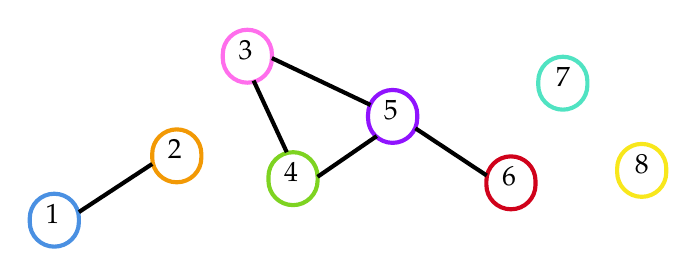
\begin{tikzpicture}[x=0.75pt,y=0.75pt,yscale=-1,xscale=1]
%uncomment if require: \path (0,300); %set diagram left start at 0, and has height of 300

%Rounded Rect [id:dp727244756598393] 
\draw  [color={rgb, 255:red, 74; green, 144; blue, 226 }  ,draw opacity=1 ][line width=1.5]  (29,137.61) .. controls (29,131.07) and (34.3,125.77) .. (40.84,125.77) -- (40.84,125.77) .. controls (47.38,125.77) and (52.68,131.07) .. (52.68,137.61) -- (52.68,139.43) .. controls (52.68,145.97) and (47.38,151.27) .. (40.84,151.27) -- (40.84,151.27) .. controls (34.3,151.27) and (29,145.97) .. (29,139.43) -- cycle ;
%Rounded Rect [id:dp693573369980472] 
\draw  [color={rgb, 255:red, 242; green, 153; blue, 5 }  ,draw opacity=1 ][line width=1.5]  (88,106.61) .. controls (88,100.07) and (93.3,94.77) .. (99.84,94.77) -- (99.84,94.77) .. controls (106.38,94.77) and (111.68,100.07) .. (111.68,106.61) -- (111.68,108.43) .. controls (111.68,114.97) and (106.38,120.27) .. (99.84,120.27) -- (99.84,120.27) .. controls (93.3,120.27) and (88,114.97) .. (88,108.43) -- cycle ;
%Rounded Rect [id:dp6295362393544817] 
\draw  [color={rgb, 255:red, 255; green, 110; blue, 236 }  ,draw opacity=1 ][line width=1.5]  (122,58.61) .. controls (122,52.07) and (127.3,46.77) .. (133.84,46.77) -- (133.84,46.77) .. controls (140.38,46.77) and (145.68,52.07) .. (145.68,58.61) -- (145.68,60.43) .. controls (145.68,66.97) and (140.38,72.27) .. (133.84,72.27) -- (133.84,72.27) .. controls (127.3,72.27) and (122,66.97) .. (122,60.43) -- cycle ;
%Rounded Rect [id:dp04815667436062654] 
\draw  [color={rgb, 255:red, 126; green, 211; blue, 33 }  ,draw opacity=1 ][line width=1.5]  (144,117.61) .. controls (144,111.07) and (149.3,105.77) .. (155.84,105.77) -- (155.84,105.77) .. controls (162.38,105.77) and (167.68,111.07) .. (167.68,117.61) -- (167.68,119.43) .. controls (167.68,125.97) and (162.38,131.27) .. (155.84,131.27) -- (155.84,131.27) .. controls (149.3,131.27) and (144,125.97) .. (144,119.43) -- cycle ;
%Rounded Rect [id:dp6930305311487936] 
\draw  [color={rgb, 255:red, 144; green, 19; blue, 254 }  ,draw opacity=1 ][line width=1.5]  (192,87.61) .. controls (192,81.07) and (197.3,75.77) .. (203.84,75.77) -- (203.84,75.77) .. controls (210.38,75.77) and (215.68,81.07) .. (215.68,87.61) -- (215.68,89.43) .. controls (215.68,95.97) and (210.38,101.27) .. (203.84,101.27) -- (203.84,101.27) .. controls (197.3,101.27) and (192,95.97) .. (192,89.43) -- cycle ;
%Rounded Rect [id:dp6372901419282468] 
\draw  [color={rgb, 255:red, 208; green, 2; blue, 27 }  ,draw opacity=1 ][line width=1.5]  (249,119.61) .. controls (249,113.07) and (254.3,107.77) .. (260.84,107.77) -- (260.84,107.77) .. controls (267.38,107.77) and (272.68,113.07) .. (272.68,119.61) -- (272.68,121.43) .. controls (272.68,127.97) and (267.38,133.27) .. (260.84,133.27) -- (260.84,133.27) .. controls (254.3,133.27) and (249,127.97) .. (249,121.43) -- cycle ;
%Rounded Rect [id:dp37697559304492145] 
\draw  [color={rgb, 255:red, 80; green, 227; blue, 194 }  ,draw opacity=1 ][line width=1.5]  (274,71.61) .. controls (274,65.07) and (279.3,59.77) .. (285.84,59.77) -- (285.84,59.77) .. controls (292.38,59.77) and (297.68,65.07) .. (297.68,71.61) -- (297.68,73.43) .. controls (297.68,79.97) and (292.38,85.27) .. (285.84,85.27) -- (285.84,85.27) .. controls (279.3,85.27) and (274,79.97) .. (274,73.43) -- cycle ;
%Rounded Rect [id:dp5534521526806271] 
\draw  [color={rgb, 255:red, 248; green, 231; blue, 28 }  ,draw opacity=1 ][line width=1.5]  (312,113.61) .. controls (312,107.07) and (317.3,101.77) .. (323.84,101.77) -- (323.84,101.77) .. controls (330.38,101.77) and (335.68,107.07) .. (335.68,113.61) -- (335.68,115.43) .. controls (335.68,121.97) and (330.38,127.27) .. (323.84,127.27) -- (323.84,127.27) .. controls (317.3,127.27) and (312,121.97) .. (312,115.43) -- cycle ;
%Straight Lines [id:da03331792259453903] 
\draw [line width=1.5]    (52.68,134.61) -- (88,111.43) ;
%Straight Lines [id:da9651033060530065] 
\draw [line width=1.5]    (152.84,105.77) -- (136.84,71.27) ;
%Straight Lines [id:da26193068858450497] 
\draw [line width=1.5]    (193.17,83) -- (145.68,60.43) ;
%Straight Lines [id:da5121704900801909] 
\draw [line width=1.5]    (167.68,117.61) -- (196.17,98) ;
%Straight Lines [id:da04948505045903029] 
\draw [line width=1.5]    (249.17,117) -- (214.84,94.27) ;

% Text Node
\draw (35.34,129.52) node [anchor=north west][inner sep=0.75pt]  [color={rgb, 255:red, 0; green, 0; blue, 0 }  ,opacity=1 ] [align=left] {\textcolor[rgb]{1,1,1}{$\displaystyle \textcolor[rgb]{0,0,0}{1}$}};
% Text Node
\draw (94.34,98.52) node [anchor=north west][inner sep=0.75pt]  [color={rgb, 255:red, 0; green, 0; blue, 0 }  ,opacity=1 ] [align=left] {\textcolor[rgb]{0,0,0}{$\displaystyle \textcolor[rgb]{0,0,0}{2}$}};
% Text Node
\draw (128.34,50.52) node [anchor=north west][inner sep=0.75pt]  [color={rgb, 255:red, 0; green, 0; blue, 0 }  ,opacity=1 ] [align=left] {\textcolor[rgb]{0,0,0}{$\displaystyle \textcolor[rgb]{0,0,0}{3}$}};
% Text Node
\draw (150.34,109.52) node [anchor=north west][inner sep=0.75pt]  [color={rgb, 255:red, 0; green, 0; blue, 0 }  ,opacity=1 ] [align=left] {\textcolor[rgb]{0,0,0}{$\displaystyle 4$}};
% Text Node
\draw (198.34,79.52) node [anchor=north west][inner sep=0.75pt]  [color={rgb, 255:red, 0; green, 0; blue, 0 }  ,opacity=1 ] [align=left] {\textcolor[rgb]{0,0,0}{$\displaystyle 5$}};
% Text Node
\draw (255.34,111.52) node [anchor=north west][inner sep=0.75pt]  [color={rgb, 255:red, 0; green, 0; blue, 0 }  ,opacity=1 ] [align=left] {\textcolor[rgb]{0,0,0}{$\displaystyle 6$}};
% Text Node
\draw (281.34,63.52) node [anchor=north west][inner sep=0.75pt]  [color={rgb, 255:red, 0; green, 0; blue, 0 }  ,opacity=1 ] [align=left] {\textcolor[rgb]{0,0,0}{$\displaystyle 7$}};
% Text Node
\draw (319.34,105.52) node [anchor=north west][inner sep=0.75pt]  [color={rgb, 255:red, 0; green, 0; blue, 0 }  ,opacity=1 ] [align=left] {\textcolor[rgb]{0,0,0}{$\displaystyle 8$}};
\end{tikzpicture}
\end{center}
On trouve que : 
\begin{itemize}
	\item	8 nœuds : $N	=	\{1, 2, 3, 4, 5, 6, 7, 8\}$.
	\item	5 arcs : $A	=	\{\{1, 2\}, \{3, 4\}, \{3, 5\}, \{4, 5\}, \{5, 6\}\}$.
	\item	4 composantes : $\{\{1, 2\}, \{3, 4, 5\}, \{7\}, \{8\}\}$.
\end{itemize}

Également, puisqu'il y a plusieurs composantes, le graphique n'est pas connecté.
\end{formula}

\begin{definitionNOHFILL}[Graphique aléatoire]
Graphique avec $n$ nœuds pour lequel deux composantes $i$ et $j$ ne sont pas reliées avec certitude, mais plutôt avec probabilité $P_{i, j}$ : 
\begin{center}
\tikzset{every picture/.style={line width=0.75pt}} %set default line width to 0.75pt        
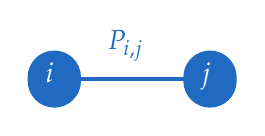
\begin{tikzpicture}[x=0.75pt,y=0.75pt,yscale=-1,xscale=1]
%uncomment if require: \path (0,112); %set diagram left start at 0, and has height of 112

%Straight Lines [id:da633468194869987] 
\draw [color={rgb, 255:red, 32; green, 106; blue, 194 }  ,draw opacity=1 ][line width=1.5]    (167.68,37.02) -- (219,37.02) ;
%Rounded Rect [id:dp6580738501830994] 
\draw  [color={rgb, 255:red, 32; green, 106; blue, 194 }  ,draw opacity=1 ][fill={rgb, 255:red, 32; green, 106; blue, 194 }  ,fill opacity=1 ][line width=1.5]  (144,36.11) .. controls (144,29.57) and (149.3,24.27) .. (155.84,24.27) -- (155.84,24.27) .. controls (162.38,24.27) and (167.68,29.57) .. (167.68,36.11) -- (167.68,37.93) .. controls (167.68,44.47) and (162.38,49.77) .. (155.84,49.77) -- (155.84,49.77) .. controls (149.3,49.77) and (144,44.47) .. (144,37.93) -- cycle ;

%Rounded Rect [id:dp18402671624270361] 
\draw  [color={rgb, 255:red, 32; green, 106; blue, 194 }  ,draw opacity=1 ][fill={rgb, 255:red, 32; green, 106; blue, 194 }  ,fill opacity=1 ][line width=1.5]  (219,36.11) .. controls (219,29.57) and (224.3,24.27) .. (230.84,24.27) -- (230.84,24.27) .. controls (237.38,24.27) and (242.68,29.57) .. (242.68,36.11) -- (242.68,37.93) .. controls (242.68,44.47) and (237.38,49.77) .. (230.84,49.77) -- (230.84,49.77) .. controls (224.3,49.77) and (219,44.47) .. (219,37.93) -- cycle ;


% Text Node
\draw (180.34,12.52) node [anchor=north west][inner sep=0.75pt]  [color={rgb, 255:red, 32; green, 106; blue, 194 }  ,opacity=1 ] [align=left] {$\displaystyle P_{i,j}$};
% Text Node
\draw (150.34,28.02) node [anchor=north west][inner sep=0.75pt]  [color={rgb, 255:red, 0; green, 0; blue, 0 }  ,opacity=1 ] [align=left] {\textcolor[rgb]{1,1,1}{$\displaystyle i$}};
% Text Node
\draw (225.34,28.02) node [anchor=north west][inner sep=0.75pt]  [color={rgb, 255:red, 0; green, 0; blue, 0 }  ,opacity=1 ] [align=left] {\textcolor[rgb]{0,0,0}{$\displaystyle \textcolor[rgb]{1,1,1}{j}$}};
\end{tikzpicture}
\end{center}

Soit la v.a. \lfbox[formula]{$X_{i, j}$} représentant l'existence d'un arc entre les nœuds $i$ et $j $ avec probabilité $\Pr(X_{i, j} = 1) = P_{i, j}$ alors : 
\begin{align*}
	X_{i, j}
	&=	\begin{cases}
		1,	&	\text{si $\{i, j\}$ est un arc}	\\
		0,	&	\text{sinon}	
		\end{cases}
\end{align*}
\end{definitionNOHFILL}

\begin{definitionNOHFILLsub}[Connectivité des graphiques aléatoiress]
\begin{rappel_enhanced}[Contexte]
La connectivité des graphiques aléatoires est semblable à la fiabilité des systèmes. \\

Pour un système, il n'est pas nécessaire que toutes les composantes fonctionnent pour que le système fonctionne. De façon semblable, il n'est pas nécessaire que tous les nœuds d'un graphique aléatoire soient reliés pour qu'il soit connecté.\\

Alors, on peut appliquer les mêmes concepts de \og \textit{minimal path sets} \fg{} et de \og \textit{minimal cut sets} \fg{} des systèmes aux graphiques aléatoires.
\end{rappel_enhanced}

Un graphique \textit{aléatoire} est connecté tant que tous les arcs d'au moins un \og \textit{minimal path sets} \fg{} existent.\\

Un graphique aléatoire de $n$ nœuds a :
\begin{itemize}
	\item	\lfbox[formula]{$n^{n - 2}$} \og \textit{minimal path sets} \fg{}, et 
	\item	\lfbox[formula]{$2^{n - 1} - 1$} \og \textit{minimal cut sets} \fg{}, 
	\item	\lfbox[formula]{$2^{\binom{n}{2}}$} graphiques possibles.
\end{itemize}
\end{definitionNOHFILLsub}

\begin{formula}{Exemple de connectivité}
Soit un graphique aléatoire avec 3 nœuds.\\

Les $3^{3 - 2} = 3$ \og \textit{minimal path sets} \fg{} sont les suivants :
\begin{center}
\tikzset{every picture/.style={line width=0.75pt}} %set default line width to 0.75pt        
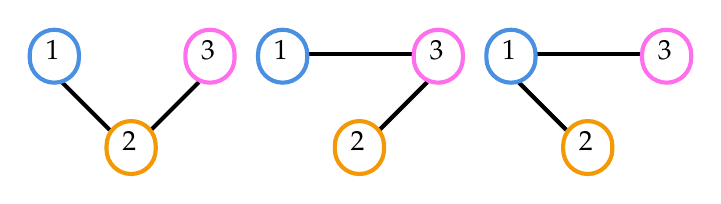
\begin{tikzpicture}[x=0.75pt,y=0.75pt,yscale=-1,xscale=1]
%uncomment if require: \path (0,112); %set diagram left start at 0, and has height of 112

%Straight Lines [id:da757165276440054] 
\draw [line width=1.5]    (72.5,72) -- (49.5,49) ;
%Straight Lines [id:da2901151971785225] 
\draw [line width=1.5]    (92.5,72) -- (115.5,49) ;
%Rounded Rect [id:dp18977091150381975] 
\draw  [color={rgb, 255:red, 74; green, 144; blue, 226 }  ,draw opacity=1 ][line width=1.5]  (34,35.61) .. controls (34,29.07) and (39.3,23.77) .. (45.84,23.77) -- (45.84,23.77) .. controls (52.38,23.77) and (57.68,29.07) .. (57.68,35.61) -- (57.68,37.43) .. controls (57.68,43.97) and (52.38,49.27) .. (45.84,49.27) -- (45.84,49.27) .. controls (39.3,49.27) and (34,43.97) .. (34,37.43) -- cycle ;

%Rounded Rect [id:dp9935301867557762] 
\draw  [color={rgb, 255:red, 242; green, 153; blue, 5 }  ,draw opacity=1 ][line width=1.5]  (71,79.61) .. controls (71,73.07) and (76.3,67.77) .. (82.84,67.77) -- (82.84,67.77) .. controls (89.38,67.77) and (94.68,73.07) .. (94.68,79.61) -- (94.68,81.43) .. controls (94.68,87.97) and (89.38,93.27) .. (82.84,93.27) -- (82.84,93.27) .. controls (76.3,93.27) and (71,87.97) .. (71,81.43) -- cycle ;

%Rounded Rect [id:dp013391070155128748] 
\draw  [color={rgb, 255:red, 255; green, 110; blue, 236 }  ,draw opacity=1 ][line width=1.5]  (109,35.61) .. controls (109,29.07) and (114.3,23.77) .. (120.84,23.77) -- (120.84,23.77) .. controls (127.38,23.77) and (132.68,29.07) .. (132.68,35.61) -- (132.68,37.43) .. controls (132.68,43.97) and (127.38,49.27) .. (120.84,49.27) -- (120.84,49.27) .. controls (114.3,49.27) and (109,43.97) .. (109,37.43) -- cycle ;

%Straight Lines [id:da8975400796076565] 
\draw [line width=1.5]    (167.68,35.43) -- (219,35.43) ;
%Straight Lines [id:da167284122584747] 
\draw [line width=1.5]    (202.5,72) -- (225.5,49) ;
%Rounded Rect [id:dp13577760592528776] 
\draw  [color={rgb, 255:red, 74; green, 144; blue, 226 }  ,draw opacity=1 ][line width=1.5]  (144,35.61) .. controls (144,29.07) and (149.3,23.77) .. (155.84,23.77) -- (155.84,23.77) .. controls (162.38,23.77) and (167.68,29.07) .. (167.68,35.61) -- (167.68,37.43) .. controls (167.68,43.97) and (162.38,49.27) .. (155.84,49.27) -- (155.84,49.27) .. controls (149.3,49.27) and (144,43.97) .. (144,37.43) -- cycle ;

%Rounded Rect [id:dp046842562867378534] 
\draw  [color={rgb, 255:red, 242; green, 153; blue, 5 }  ,draw opacity=1 ][line width=1.5]  (181,79.61) .. controls (181,73.07) and (186.3,67.77) .. (192.84,67.77) -- (192.84,67.77) .. controls (199.38,67.77) and (204.68,73.07) .. (204.68,79.61) -- (204.68,81.43) .. controls (204.68,87.97) and (199.38,93.27) .. (192.84,93.27) -- (192.84,93.27) .. controls (186.3,93.27) and (181,87.97) .. (181,81.43) -- cycle ;

%Rounded Rect [id:dp05685675073164731] 
\draw  [color={rgb, 255:red, 255; green, 110; blue, 236 }  ,draw opacity=1 ][line width=1.5]  (219,35.61) .. controls (219,29.07) and (224.3,23.77) .. (230.84,23.77) -- (230.84,23.77) .. controls (237.38,23.77) and (242.68,29.07) .. (242.68,35.61) -- (242.68,37.43) .. controls (242.68,43.97) and (237.38,49.27) .. (230.84,49.27) -- (230.84,49.27) .. controls (224.3,49.27) and (219,43.97) .. (219,37.43) -- cycle ;

%Straight Lines [id:da15700560076822256] 
\draw [line width=1.5]    (277.68,35.43) -- (329,35.43) ;
%Straight Lines [id:da5100726311758725] 
\draw [line width=1.5]    (292.5,72) -- (269.5,49) ;
%Rounded Rect [id:dp9633502813554886] 
\draw  [color={rgb, 255:red, 74; green, 144; blue, 226 }  ,draw opacity=1 ][line width=1.5]  (254,35.61) .. controls (254,29.07) and (259.3,23.77) .. (265.84,23.77) -- (265.84,23.77) .. controls (272.38,23.77) and (277.68,29.07) .. (277.68,35.61) -- (277.68,37.43) .. controls (277.68,43.97) and (272.38,49.27) .. (265.84,49.27) -- (265.84,49.27) .. controls (259.3,49.27) and (254,43.97) .. (254,37.43) -- cycle ;

%Rounded Rect [id:dp43956572400381333] 
\draw  [color={rgb, 255:red, 242; green, 153; blue, 5 }  ,draw opacity=1 ][line width=1.5]  (291,79.61) .. controls (291,73.07) and (296.3,67.77) .. (302.84,67.77) -- (302.84,67.77) .. controls (309.38,67.77) and (314.68,73.07) .. (314.68,79.61) -- (314.68,81.43) .. controls (314.68,87.97) and (309.38,93.27) .. (302.84,93.27) -- (302.84,93.27) .. controls (296.3,93.27) and (291,87.97) .. (291,81.43) -- cycle ;

%Rounded Rect [id:dp4418103150222692] 
\draw  [color={rgb, 255:red, 255; green, 110; blue, 236 }  ,draw opacity=1 ][line width=1.5]  (329,35.61) .. controls (329,29.07) and (334.3,23.77) .. (340.84,23.77) -- (340.84,23.77) .. controls (347.38,23.77) and (352.68,29.07) .. (352.68,35.61) -- (352.68,37.43) .. controls (352.68,43.97) and (347.38,49.27) .. (340.84,49.27) -- (340.84,49.27) .. controls (334.3,49.27) and (329,43.97) .. (329,37.43) -- cycle ;


% Text Node
\draw (40.34,27.52) node [anchor=north west][inner sep=0.75pt]  [color={rgb, 255:red, 0; green, 0; blue, 0 }  ,opacity=1 ] [align=left] {\textcolor[rgb]{1,1,1}{$\displaystyle \textcolor[rgb]{0,0,0}{1}$}};
% Text Node
\draw (77.34,71.52) node [anchor=north west][inner sep=0.75pt]  [color={rgb, 255:red, 0; green, 0; blue, 0 }  ,opacity=1 ] [align=left] {\textcolor[rgb]{0,0,0}{$\displaystyle \textcolor[rgb]{0,0,0}{2}$}};
% Text Node
\draw (115.34,27.52) node [anchor=north west][inner sep=0.75pt]  [color={rgb, 255:red, 0; green, 0; blue, 0 }  ,opacity=1 ] [align=left] {\textcolor[rgb]{0,0,0}{$\displaystyle \textcolor[rgb]{0,0,0}{3}$}};
% Text Node
\draw (225.34,27.52) node [anchor=north west][inner sep=0.75pt]  [color={rgb, 255:red, 0; green, 0; blue, 0 }  ,opacity=1 ] [align=left] {\textcolor[rgb]{0,0,0}{$\displaystyle \textcolor[rgb]{0,0,0}{3}$}};
% Text Node
\draw (187.34,71.52) node [anchor=north west][inner sep=0.75pt]  [color={rgb, 255:red, 0; green, 0; blue, 0 }  ,opacity=1 ] [align=left] {\textcolor[rgb]{0,0,0}{$\displaystyle \textcolor[rgb]{0,0,0}{2}$}};
% Text Node
\draw (150.34,27.52) node [anchor=north west][inner sep=0.75pt]  [color={rgb, 255:red, 0; green, 0; blue, 0 }  ,opacity=1 ] [align=left] {\textcolor[rgb]{1,1,1}{$\displaystyle \textcolor[rgb]{0,0,0}{1}$}};
% Text Node
\draw (335.34,27.52) node [anchor=north west][inner sep=0.75pt]  [color={rgb, 255:red, 0; green, 0; blue, 0 }  ,opacity=1 ] [align=left] {\textcolor[rgb]{0,0,0}{$\displaystyle \textcolor[rgb]{0,0,0}{3}$}};
% Text Node
\draw (297.34,71.52) node [anchor=north west][inner sep=0.75pt]  [color={rgb, 255:red, 0; green, 0; blue, 0 }  ,opacity=1 ] [align=left] {\textcolor[rgb]{0,0,0}{$\displaystyle \textcolor[rgb]{0,0,0}{2}$}};
% Text Node
\draw (260.34,27.52) node [anchor=north west][inner sep=0.75pt]  [color={rgb, 255:red, 0; green, 0; blue, 0 }  ,opacity=1 ] [align=left] {\textcolor[rgb]{1,1,1}{$\displaystyle \textcolor[rgb]{0,0,0}{1}$}};
\end{tikzpicture}
\end{center}

Les $2^{3 - 1} - 1 = 3$ \og \textit{minimal cut sets} \fg{} sont les suivants :
\begin{center}
\tikzset{every picture/.style={line width=0.75pt}} %set default line width to 0.75pt        
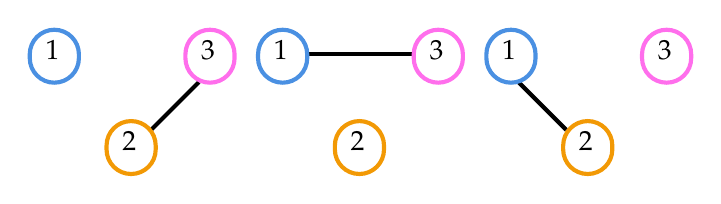
\begin{tikzpicture}[x=0.75pt,y=0.75pt,yscale=-1,xscale=1]
%uncomment if require: \path (0,112); %set diagram left start at 0, and has height of 112

%Straight Lines [id:da7347161419448469] 
\draw [line width=1.5]    (92.5,72) -- (115.5,49) ;
%Rounded Rect [id:dp52812847367501] 
\draw  [color={rgb, 255:red, 74; green, 144; blue, 226 }  ,draw opacity=1 ][line width=1.5]  (34,35.61) .. controls (34,29.07) and (39.3,23.77) .. (45.84,23.77) -- (45.84,23.77) .. controls (52.38,23.77) and (57.68,29.07) .. (57.68,35.61) -- (57.68,37.43) .. controls (57.68,43.97) and (52.38,49.27) .. (45.84,49.27) -- (45.84,49.27) .. controls (39.3,49.27) and (34,43.97) .. (34,37.43) -- cycle ;

%Rounded Rect [id:dp5617743459291145] 
\draw  [color={rgb, 255:red, 242; green, 153; blue, 5 }  ,draw opacity=1 ][line width=1.5]  (71,79.61) .. controls (71,73.07) and (76.3,67.77) .. (82.84,67.77) -- (82.84,67.77) .. controls (89.38,67.77) and (94.68,73.07) .. (94.68,79.61) -- (94.68,81.43) .. controls (94.68,87.97) and (89.38,93.27) .. (82.84,93.27) -- (82.84,93.27) .. controls (76.3,93.27) and (71,87.97) .. (71,81.43) -- cycle ;

%Rounded Rect [id:dp008376903551648773] 
\draw  [color={rgb, 255:red, 255; green, 110; blue, 236 }  ,draw opacity=1 ][line width=1.5]  (109,35.61) .. controls (109,29.07) and (114.3,23.77) .. (120.84,23.77) -- (120.84,23.77) .. controls (127.38,23.77) and (132.68,29.07) .. (132.68,35.61) -- (132.68,37.43) .. controls (132.68,43.97) and (127.38,49.27) .. (120.84,49.27) -- (120.84,49.27) .. controls (114.3,49.27) and (109,43.97) .. (109,37.43) -- cycle ;

%Straight Lines [id:da7905063435136956] 
\draw [line width=1.5]    (167.68,35.43) -- (219,35.43) ;
%Rounded Rect [id:dp2938655868030775] 
\draw  [color={rgb, 255:red, 74; green, 144; blue, 226 }  ,draw opacity=1 ][line width=1.5]  (144,35.61) .. controls (144,29.07) and (149.3,23.77) .. (155.84,23.77) -- (155.84,23.77) .. controls (162.38,23.77) and (167.68,29.07) .. (167.68,35.61) -- (167.68,37.43) .. controls (167.68,43.97) and (162.38,49.27) .. (155.84,49.27) -- (155.84,49.27) .. controls (149.3,49.27) and (144,43.97) .. (144,37.43) -- cycle ;

%Rounded Rect [id:dp8911373398860187] 
\draw  [color={rgb, 255:red, 242; green, 153; blue, 5 }  ,draw opacity=1 ][line width=1.5]  (181,79.61) .. controls (181,73.07) and (186.3,67.77) .. (192.84,67.77) -- (192.84,67.77) .. controls (199.38,67.77) and (204.68,73.07) .. (204.68,79.61) -- (204.68,81.43) .. controls (204.68,87.97) and (199.38,93.27) .. (192.84,93.27) -- (192.84,93.27) .. controls (186.3,93.27) and (181,87.97) .. (181,81.43) -- cycle ;

%Rounded Rect [id:dp11220105471499431] 
\draw  [color={rgb, 255:red, 255; green, 110; blue, 236 }  ,draw opacity=1 ][line width=1.5]  (219,35.61) .. controls (219,29.07) and (224.3,23.77) .. (230.84,23.77) -- (230.84,23.77) .. controls (237.38,23.77) and (242.68,29.07) .. (242.68,35.61) -- (242.68,37.43) .. controls (242.68,43.97) and (237.38,49.27) .. (230.84,49.27) -- (230.84,49.27) .. controls (224.3,49.27) and (219,43.97) .. (219,37.43) -- cycle ;

%Straight Lines [id:da5084894535194546] 
\draw [line width=1.5]    (292.5,72) -- (269.5,49) ;
%Rounded Rect [id:dp14491739390865632] 
\draw  [color={rgb, 255:red, 74; green, 144; blue, 226 }  ,draw opacity=1 ][line width=1.5]  (254,35.61) .. controls (254,29.07) and (259.3,23.77) .. (265.84,23.77) -- (265.84,23.77) .. controls (272.38,23.77) and (277.68,29.07) .. (277.68,35.61) -- (277.68,37.43) .. controls (277.68,43.97) and (272.38,49.27) .. (265.84,49.27) -- (265.84,49.27) .. controls (259.3,49.27) and (254,43.97) .. (254,37.43) -- cycle ;

%Rounded Rect [id:dp8766875618692331] 
\draw  [color={rgb, 255:red, 242; green, 153; blue, 5 }  ,draw opacity=1 ][line width=1.5]  (291,79.61) .. controls (291,73.07) and (296.3,67.77) .. (302.84,67.77) -- (302.84,67.77) .. controls (309.38,67.77) and (314.68,73.07) .. (314.68,79.61) -- (314.68,81.43) .. controls (314.68,87.97) and (309.38,93.27) .. (302.84,93.27) -- (302.84,93.27) .. controls (296.3,93.27) and (291,87.97) .. (291,81.43) -- cycle ;

%Rounded Rect [id:dp40232492134805176] 
\draw  [color={rgb, 255:red, 255; green, 110; blue, 236 }  ,draw opacity=1 ][line width=1.5]  (329,35.61) .. controls (329,29.07) and (334.3,23.77) .. (340.84,23.77) -- (340.84,23.77) .. controls (347.38,23.77) and (352.68,29.07) .. (352.68,35.61) -- (352.68,37.43) .. controls (352.68,43.97) and (347.38,49.27) .. (340.84,49.27) -- (340.84,49.27) .. controls (334.3,49.27) and (329,43.97) .. (329,37.43) -- cycle ;


% Text Node
\draw (40.34,27.52) node [anchor=north west][inner sep=0.75pt]  [color={rgb, 255:red, 0; green, 0; blue, 0 }  ,opacity=1 ] [align=left] {\textcolor[rgb]{1,1,1}{$\displaystyle \textcolor[rgb]{0,0,0}{1}$}};
% Text Node
\draw (77.34,71.52) node [anchor=north west][inner sep=0.75pt]  [color={rgb, 255:red, 0; green, 0; blue, 0 }  ,opacity=1 ] [align=left] {\textcolor[rgb]{0,0,0}{$\displaystyle \textcolor[rgb]{0,0,0}{2}$}};
% Text Node
\draw (115.34,27.52) node [anchor=north west][inner sep=0.75pt]  [color={rgb, 255:red, 0; green, 0; blue, 0 }  ,opacity=1 ] [align=left] {\textcolor[rgb]{0,0,0}{$\displaystyle \textcolor[rgb]{0,0,0}{3}$}};
% Text Node
\draw (225.34,27.52) node [anchor=north west][inner sep=0.75pt]  [color={rgb, 255:red, 0; green, 0; blue, 0 }  ,opacity=1 ] [align=left] {\textcolor[rgb]{0,0,0}{$\displaystyle \textcolor[rgb]{0,0,0}{3}$}};
% Text Node
\draw (187.34,71.52) node [anchor=north west][inner sep=0.75pt]  [color={rgb, 255:red, 0; green, 0; blue, 0 }  ,opacity=1 ] [align=left] {\textcolor[rgb]{0,0,0}{$\displaystyle \textcolor[rgb]{0,0,0}{2}$}};
% Text Node
\draw (150.34,27.52) node [anchor=north west][inner sep=0.75pt]  [color={rgb, 255:red, 0; green, 0; blue, 0 }  ,opacity=1 ] [align=left] {\textcolor[rgb]{1,1,1}{$\displaystyle \textcolor[rgb]{0,0,0}{1}$}};
% Text Node
\draw (335.34,27.52) node [anchor=north west][inner sep=0.75pt]  [color={rgb, 255:red, 0; green, 0; blue, 0 }  ,opacity=1 ] [align=left] {\textcolor[rgb]{0,0,0}{$\displaystyle \textcolor[rgb]{0,0,0}{3}$}};
% Text Node
\draw (297.34,71.52) node [anchor=north west][inner sep=0.75pt]  [color={rgb, 255:red, 0; green, 0; blue, 0 }  ,opacity=1 ] [align=left] {\textcolor[rgb]{0,0,0}{$\displaystyle \textcolor[rgb]{0,0,0}{2}$}};
% Text Node
\draw (260.34,27.52) node [anchor=north west][inner sep=0.75pt]  [color={rgb, 255:red, 0; green, 0; blue, 0 }  ,opacity=1 ] [align=left] {\textcolor[rgb]{1,1,1}{$\displaystyle \textcolor[rgb]{0,0,0}{1}$}};
\end{tikzpicture}
\end{center}

Les deux autres graphiques possibles qui ne sont pas optimaux sont : 
\begin{center}
\tikzset{every picture/.style={line width=0.75pt}} %set default line width to 0.75pt        
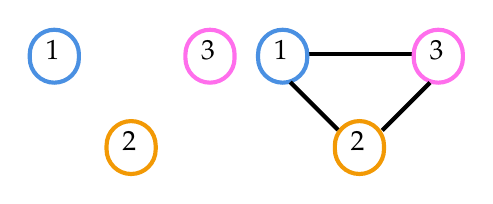
\begin{tikzpicture}[x=0.75pt,y=0.75pt,yscale=-1,xscale=1]
%uncomment if require: \path (0,112); %set diagram left start at 0, and has height of 112

%Rounded Rect [id:dp026022160743957468] 
\draw  [color={rgb, 255:red, 74; green, 144; blue, 226 }  ,draw opacity=1 ][line width=1.5]  (34,35.61) .. controls (34,29.07) and (39.3,23.77) .. (45.84,23.77) -- (45.84,23.77) .. controls (52.38,23.77) and (57.68,29.07) .. (57.68,35.61) -- (57.68,37.43) .. controls (57.68,43.97) and (52.38,49.27) .. (45.84,49.27) -- (45.84,49.27) .. controls (39.3,49.27) and (34,43.97) .. (34,37.43) -- cycle ;

%Rounded Rect [id:dp05719591207338426] 
\draw  [color={rgb, 255:red, 242; green, 153; blue, 5 }  ,draw opacity=1 ][line width=1.5]  (71,79.61) .. controls (71,73.07) and (76.3,67.77) .. (82.84,67.77) -- (82.84,67.77) .. controls (89.38,67.77) and (94.68,73.07) .. (94.68,79.61) -- (94.68,81.43) .. controls (94.68,87.97) and (89.38,93.27) .. (82.84,93.27) -- (82.84,93.27) .. controls (76.3,93.27) and (71,87.97) .. (71,81.43) -- cycle ;

%Rounded Rect [id:dp36049870395542616] 
\draw  [color={rgb, 255:red, 255; green, 110; blue, 236 }  ,draw opacity=1 ][line width=1.5]  (109,35.61) .. controls (109,29.07) and (114.3,23.77) .. (120.84,23.77) -- (120.84,23.77) .. controls (127.38,23.77) and (132.68,29.07) .. (132.68,35.61) -- (132.68,37.43) .. controls (132.68,43.97) and (127.38,49.27) .. (120.84,49.27) -- (120.84,49.27) .. controls (114.3,49.27) and (109,43.97) .. (109,37.43) -- cycle ;

%Straight Lines [id:da9797441095435544] 
\draw [line width=1.5]    (167.68,35.43) -- (219,35.43) ;
%Rounded Rect [id:dp6836288115751512] 
\draw  [color={rgb, 255:red, 74; green, 144; blue, 226 }  ,draw opacity=1 ][line width=1.5]  (144,35.61) .. controls (144,29.07) and (149.3,23.77) .. (155.84,23.77) -- (155.84,23.77) .. controls (162.38,23.77) and (167.68,29.07) .. (167.68,35.61) -- (167.68,37.43) .. controls (167.68,43.97) and (162.38,49.27) .. (155.84,49.27) -- (155.84,49.27) .. controls (149.3,49.27) and (144,43.97) .. (144,37.43) -- cycle ;

%Rounded Rect [id:dp29789997781466515] 
\draw  [color={rgb, 255:red, 242; green, 153; blue, 5 }  ,draw opacity=1 ][line width=1.5]  (181,79.61) .. controls (181,73.07) and (186.3,67.77) .. (192.84,67.77) -- (192.84,67.77) .. controls (199.38,67.77) and (204.68,73.07) .. (204.68,79.61) -- (204.68,81.43) .. controls (204.68,87.97) and (199.38,93.27) .. (192.84,93.27) -- (192.84,93.27) .. controls (186.3,93.27) and (181,87.97) .. (181,81.43) -- cycle ;

%Rounded Rect [id:dp5750339472332271] 
\draw  [color={rgb, 255:red, 255; green, 110; blue, 236 }  ,draw opacity=1 ][line width=1.5]  (219,35.61) .. controls (219,29.07) and (224.3,23.77) .. (230.84,23.77) -- (230.84,23.77) .. controls (237.38,23.77) and (242.68,29.07) .. (242.68,35.61) -- (242.68,37.43) .. controls (242.68,43.97) and (237.38,49.27) .. (230.84,49.27) -- (230.84,49.27) .. controls (224.3,49.27) and (219,43.97) .. (219,37.43) -- cycle ;

%Straight Lines [id:da2732284992251657] 
\draw [line width=1.5]    (182.5,72) -- (159.5,49) ;
%Straight Lines [id:da787308110865319] 
\draw [line width=1.5]    (203.84,72.27) -- (217.51,58.6) -- (226.84,49.27) ;

% Text Node
\draw (40.34,27.52) node [anchor=north west][inner sep=0.75pt]  [color={rgb, 255:red, 0; green, 0; blue, 0 }  ,opacity=1 ] [align=left] {\textcolor[rgb]{1,1,1}{$\displaystyle \textcolor[rgb]{0,0,0}{1}$}};
% Text Node
\draw (77.34,71.52) node [anchor=north west][inner sep=0.75pt]  [color={rgb, 255:red, 0; green, 0; blue, 0 }  ,opacity=1 ] [align=left] {\textcolor[rgb]{0,0,0}{$\displaystyle \textcolor[rgb]{0,0,0}{2}$}};
% Text Node
\draw (115.34,27.52) node [anchor=north west][inner sep=0.75pt]  [color={rgb, 255:red, 0; green, 0; blue, 0 }  ,opacity=1 ] [align=left] {\textcolor[rgb]{0,0,0}{$\displaystyle \textcolor[rgb]{0,0,0}{3}$}};
% Text Node
\draw (225.34,27.52) node [anchor=north west][inner sep=0.75pt]  [color={rgb, 255:red, 0; green, 0; blue, 0 }  ,opacity=1 ] [align=left] {\textcolor[rgb]{0,0,0}{$\displaystyle \textcolor[rgb]{0,0,0}{3}$}};
% Text Node
\draw (187.34,71.52) node [anchor=north west][inner sep=0.75pt]  [color={rgb, 255:red, 0; green, 0; blue, 0 }  ,opacity=1 ] [align=left] {\textcolor[rgb]{0,0,0}{$\displaystyle \textcolor[rgb]{0,0,0}{2}$}};
% Text Node
\draw (150.34,27.52) node [anchor=north west][inner sep=0.75pt]  [color={rgb, 255:red, 0; green, 0; blue, 0 }  ,opacity=1 ] [align=left] {\textcolor[rgb]{1,1,1}{$\displaystyle \textcolor[rgb]{0,0,0}{1}$}};
\end{tikzpicture}
\end{center}
\end{formula}

\begin{definitionNOHFILLprop}[Probabilités de connectivité des graphiques]
On pose que chaque v.a. est iid avec \lfbox[conditions]{$P_{i, j} = p$}. \\

Alors, on trouve la probabilité \lfbox[formula]{$P_{n}$} qu'un graphique aléatoire de $n$ nœuds soit connecté avec la formule récursive :
\begin{align*}
	P_{n}
	&=	1 - \sum_{k = 1}^{n - 1}\binom{n - 1}{k - 1} (1 - p)^{k(n - k)}P_{k}, \quad n = 2, 3, \dots
\end{align*}
où \lfbox[conditions]{$P_{1} = 1, P_{2} = p$}.

\tcbline

On peut également trouver les \textbf{bornes} pour la probabilité pour simplifier la tâche : 
\begin{align*}
	n(1 - p)^{n - 1} - \binom{n}{2} (1 - p)^{2n - 3}	
	\leq	1 - P_{n}		\leq	
	(n + 1) (1 - p)^{n - 1}
\end{align*}

\tcbline

Finalement, on peut \textbf{approximer} la probabilité avec \lfbox[formula]{$P_{n} \approx 1 - n(1 - p)^{n - 1}$}.
\end{definitionNOHFILLprop}


\columnbreak
\subsection{Durée de vie des systèmes}
\begin{rappel_enhanced}[Contexte]
Nous avons évalué la \textbf{\textit{fiabilité}} d'un système et comment qu'elle est impactée par la fiabilité de ses composantes.\\

Nous évaluons maintenant la \textbf{durée de vie} d'un système et comment qu'elle est impactée par la durée de vie de ses composantes.
\end{rappel_enhanced}

\begin{distributions}[Notation]
\begin{description}
	\item[$T_{i}$]	Durée de vie de la composante $i$.
	\item[$S_{i}(t)$]	Fonction de survie de la durée de vie de la composante $i$.
		\begin{itemize}
		\item	$\bm{S}(t)	=	\left(S_{1}(t), \dots, S_{n}(t)\right)$ est le vecteur des fonctions de survie des $n$ composantes.
		\end{itemize}
	\item[$T$]	Durée de vie du système.
\end{description}
\end{distributions}

\begin{definitionNOHFILLprop}[Calcul de probabilités de durée de vie]
La probabilité que le système fonctionne passé $t$ équivaut à la fonction de fiabilité évaluée au vecteur des fonctions de survie : \lfbox[formula]{$\Pr(T > t) = r[\bm{S}(t)]$}.\\

Donc, on pose $p_{i}	=	S_{i}(t)$ pour $i = 1, 2, \dots, n$.
\end{definitionNOHFILLprop}

\begin{definitionNOHFILLprop}[Espérance de durée de vie]
La durée de vie espérée équivaut à \lfbox[formula]{$\text{E}[T]	 = \int_{0}^{\infty} r[\bm{S}(t)] dt$}.
\end{definitionNOHFILLprop}

\begin{formula}{Exemple du calcul de la durée de vie espérée}
On reprend l'exemple de la sous-section sur les fonctions de fiabilité avec le système en parallèle ayant 3 composantes. \\

On pose que les 3 composantes sont indépendantes et que la durée de vie est uniformément distribuée sur $(0, 2)$.

\begin{enumerate}[label = \rectangled{\arabic*}{lightgray}]
	\item	Trouver la fonction de survie de la composante $i$ :
		\begin{align*}
		S_{i}(t)
		&=	\frac{2 - t}{2 - 0}
		=	\frac{2 - t}{2}
		\end{align*}
	\item	Trouver la fonction de fiabilité.
		\begin{itemize}
		\item	Précédemment, nous avons trouvé que $r(\bm{p}) = p_{3} + p_{1}p_{2} - p_{1}p_{2}p_{3}$.
		\end{itemize}
	\item	Remplacer $\bm{p}$ par $\bm{S}(t)$ :
		\begin{align*}
		r(\bm{p}) 
		&=	\bm{S}_{3}(t) + \bm{S}_{1}(t)\bm{S}_{2}(t) - \bm{S}_{1}(t)\bm{S}_{2}(t)\bm{S}_{3}(t)	\\
		&=	\left(\frac{2 - t}{2}\right) + \left(\frac{2 - t}{2}\right)^{2} - \left(\frac{2 - t}{2}\right)^{3}	\\
		&=	\frac{t^{3} - 4t^{2} + 8}{8}
		\end{align*}
	\item	Trouver $\text{E}[T]	$ : 
		\begin{align*}
		\text{E}[T]
		&=	\int_{0}^{2} \frac{t^{3} - 4t^{2} + 8}{8} dt	\\
		&=	1.1667
		\end{align*}
\end{enumerate}
\end{formula}

\begin{definitionNOHFILLpropos}[Étapes du calcul de probabilités, ou de l'espérance, de la durée de vie]
\begin{enumerate}[label	=	\circled{\arabic*}{trueblue}]
	\item	Déterminer la fonction de la structure du système $\phi(\bm{X})$.
		\begin{itemize}
		\item	Soit avec les \og \textit{minimal path sets} \fg{} ou les \og \textit{minimal cut sets} \fg{}.
		\end{itemize}
	\item	Déduire la fonction de fiabilité.
		\begin{itemize}
		\item	Soit en trouvant $r(\bm{p}) = \text{E}[\phi(\bm{X})]$, ou avec $r(\bm{p}) = Pr(\phi(\bm{X}) = 1)$.
		\end{itemize}
	\item	Développer la fonction de survie $\Pr(T > t)$ de la fonction de fiabilité $r(\bm{S}(t))$.
	\item	Trouver la probabilité désirée ou l'espérance.
\end{enumerate}
\end{definitionNOHFILLpropos}

\paragraph{Raccourci}	Pour un système de $k$ parmi $n$ avec des durées de vie iid suivant une loi exponentielle de moyenne $\mu$, \lfbox[formula]{$\text{E}[T]	=	\mu \sum_{i = k}^{n} \frac{1}{i}$}. Cette formule découle du coût espéré total pour les algorithmes \og \textit{greedy} \fg{} A et B.


\columnbreak
\subsection{Divers}
\label{subsec:reliabilityVaria}
\begin{rappel}{Rappel : fonction de hasard}
Dans le chapitre de \textit{\underline{\nameref{chapt:mathIARD}}} à la sous-section \textit{\underline{\nameref{subsec:rvfunct}}} on a : 
\begin{itemize}
	\item	La fonction de hasard \lfbox[formula]{$h_{X}(x)	=	\frac{f(x)}{S(x)}$}
	\item	La fonction de hasard cumulative \lfbox[formula]{$H_{X}(x)	=	\int_{-\infty}^{x}h(t)dt$}
\end{itemize}
\end{rappel}

\begin{rappel}{Système monotone}
La fiabilité du système augmente lorsque la fiabilité de toute composante augmente.
\end{rappel}

\begin{distributions}[Terminologie]
\begin{description}
	\item[IFR]	\og \textit{Increasing failure rate distribution} \fg{}.
	\item[DFR]	\og \textit{Decreasing failure rate distribution} \fg{}.
	\item[IFRA]	\og \textit{Increasing failure rate on the average distribution} \fg{}.
		\begin{itemize}
		\item	La distribution IFRA est une généralisation de la distribution IFR.
		\item	Il s'ensuit que si une distribution est IFR elle est également IFRA.
		\end{itemize}
\end{description}
\end{distributions}

\begin{center}
\begin{tabular}{| >{\columncolor{beaublue}}c | >{\columncolor{beaublue}}c  |}
\hline\rowcolor{airforceblue} 	
\rowcolor{airforceblue}\textcolor{white}{\textbf{Distribution}}	&	\textcolor{white}{$h(x)$ est une fonction $\rule{1cm}{0.15mm}$ de $x$}	\\\specialrule{0.1em}{0em}{0em} 
IFR			&	croissante		\\\hline
DFR			&	décroissante		\\\hline
IFR et DFR	&	constante		\\\hline
\end{tabular}
\end{center}

Une distribution est IFRA si $\frac{H(x)}{x}$ est une fonction \textit{croissante} de $x$, pour tout $x \geq 0$.
\paragraph{Note} Si les distribution de durées de vies de toutes les composantes (\textit{indépendantes}) d'un \textit{système monotone} sont IFRA, alors la distribution de la durée de vie du système le sera aussi. 



\subsubsection{Distributions particulières}
Puisque la fonction de hasard de la distribution exponentielle est fixe, elle est à la fois IFR et DFR. \\

Cependant, lorsque la fonction de hasard varie, le type de distribution peut varier aussi. Par exemple, pour la loi gamma et la loi de Weibull : 
\begin{center}
\begin{tabular}{| >{\columncolor{beaublue}}c | >{\columncolor{beaublue}}c  | >{\columncolor{beaublue}}c  |}
\hline\rowcolor{airforceblue} 
	&	\textcolor{white}{Weibull$(\tau, \theta)$}	&	\textcolor{white}{Gamma$(\alpha, \beta)$}		\\\cline{2-3}
\rowcolor{airforceblue}\multirow{-2}{*}{\textcolor{white}{\textbf{Distribution}}}	&	\multicolumn{2}{c|}{\textcolor{white}{\textbf{Condition}}}	\\\specialrule{0.1em}{0em}{0em} 
IFR			&	$\tau \geq 1$		&	$\alpha \geq 1$		\\\hline
DFR			&	$0 < \tau \leq 1$	&	$0 < \alpha \leq 1$	\\\hline
IFR et DFR	&	$\tau = 1$			&	$\alpha = 1$			\\\hline
\end{tabular}
\end{center}
\paragraph{Note}	Une loi gamma avec $\alpha = 1$, tout comme une loi de Weibull avec $\tau = 1$, revient à une distribution exponentielle.

\paragraph{Note}	Voir la sous-section \textit{\underline{\nameref{subsec:distrIARD}}} du chapitre de \textit{\underline{\nameref{chapt:mathIARD}}} pour une description de la loi gamma et de la loi de Weibull.





\newpage
\section{Assurance vie}
\subsection{Probabilités}
\begin{distributions}[Notation]
\begin{description}
	\item[$\ell_{\textcolor{teal}{a}}$]	Nombre d'individus initial dans une cohorte où $\textcolor{teal}{a = 0}$ habituellement.
	\item[$\ell_{x + \textcolor{teal}{a}}$]	Nombre d'individus de la cohorte ayant survécu $x$ années de $\textcolor{teal}{a}$ (donc âgés de $x + \textcolor{teal}{a}$ années).
	\item[$\prescript{}{t}d_{x}$]	Nombre de décès entre les âges $x$ et $x + t$.
		\begin{itemize}
		\item	\lfbox[formula]{$\actsymb[t]{d}{x} = l_{x} - l_{x + t}$}.
		\end{itemize}
\end{description}
\end{distributions}

\begin{definitionNOHFILLsub}[Probabilité de survie]
La probabilité qu'un assuré de $x$ ans survie au moins $t$ années est \lfbox[formula]{$\px[t]{x} = \frac{l_{x + t}}{l_{x}}$}.
\end{definitionNOHFILLsub}

\begin{definitionNOHFILLsub}[Probabilité de décès]
La probabilité qu'un assuré de $x$ ans décède d'ici $t$ années est \lfbox[formula]{$\qx[t]{x} = \frac{l_{x} - l_{x + t}}{l_{x}}$}.
\end{definitionNOHFILLsub}


\begin{definitionNOHFILL}[Variable aléatoire du nombre de décédés entre les âges $x$ et $x + t$ $\prescript{}{t}{\mathcal{D}}_{x}$]
On a que \lfbox[formula]{$\Dx[t]{x} \sim \text{Bin}(\ell_{x}, \qx[t]{x})$}.

\begin{itemize}
	\item	Il s'ensuit que $\text{E}[\Dx[t]{x}] = \dx[t]{x}$.
	\item	Également, $\Dx[t]{x} = \mathscr{L}_{x} - \mathscr{L}_{x + t}$.
\end{itemize}
\end{definitionNOHFILL}


\subsubsection{Espérances de vie}
\setlength{\mathindent}{-1cm}
\begin{definitionNOHFILLsub}[Espérance de vie \textbf{\underline{abrégée}} pour un individu d'âge $x$]
\begin{align*}
	e_{x}
	&=	\sum_{k = 0}^{\omega - x - 1} k \ \qx[k | ]{x}	\\
\end{align*}
puis, si $\limz{k}{\infty} (k + 1) \px[k + 1]{x} = 0$, 
\begin{align*}
	&=	\sum_{k = 1}^{\omega - x} \px[k]{x}
\end{align*}

\begin{itemize}
	\item	En anglais, \og \textit{\textbf{curtate life expectancy}} \fg{}.
\end{itemize}
\end{definitionNOHFILLsub}
\setlength{\mathindent}{1cm}



\setlength{\mathindent}{-1cm}
\begin{definitionNOHFILLsub}[Espérance de vie \textbf{\underline{complète}} pour un individu d'âge $x$]
\begin{align*}
	\eringx{x}
	&=	\int_{0}^{\omega - x} t \px[t]{x} \mu_{x + t} dt	\\
	&=	\int_{0}^{\omega - x} \px[t]{x} dt	\qquad\qquad\quad\quad	\text{si } \limz{t}{\infty} t \px[t]{x} = 0
\end{align*}

Sous l'hypothèse d'une distribution uniforme des décès (DUD), \lfbox[formula]{$\eringx{x} \overset{DUD}{=} e_x + \frac{1}{2}$}.

\begin{itemize}
	\item	En anglais, \og \textit{\textbf{complete expectation of life}} \fg{}.
\end{itemize}
\end{definitionNOHFILLsub}


\columnbreak
\subsection{Contrats d'assurance vie}
\begin{distributions}[Notation]
\begin{description}
	\item[$Z_{x}$]	Variable aléatoire du contrat d'assurance pour un assuré d'âge $x$.
	\item[$Y_{x}$]	Variable aléatoire de la rente pour un rentier d'âge $x$.
\end{description}
\end{distributions}


\begin{definitionNOHFILL}[Valeur présente actuarielle]
On nomme l'actualisation de paiements conditionnels à la mortalité la \textit{\textbf{valeur présente actuarielle (VPA)}}. \\

Pour des contrats d'assurance, on la dénote par $A_{x}$ et pour des contrats de rentes, par $a_{x}$.

\begin{itemize}
	\item	En anglais, \og \textit{Actuarial Present Value (APV)} \fg{}
\end{itemize}
\end{definitionNOHFILL}


\begin{definitionNOHFILLsub}[Assurance-vie entière $Z_{x}$]
Est en vigueur tant que l'assuré est en vie et verse une prestation à la fin moment de l'année de son décès.

\begin{align*}
	\Ax{x}	
	&=	\sum_{k = 0}^{\omega - x - 1} v^{k + 1} \px[k]{x} \qx{x + k} \\
	&=	v\qx{x} + v^{2}\px{x}\qx{x + 1} + v^{3}\px[2]{x}\qx{x + 2} + \dots
%	=	v\qx{x} + v\px{x}\Ax{x + 1}
\end{align*}
\end{definitionNOHFILLsub}


\begin{definitionNOHFILLsub}[Capital différé de $t$ années $\Ex[t]{x}$]
Si l'assuré \textbf{\textit{ne décède pas}} dans les $t$ années suivant l'émission du contrat, le capital différé $\Ex[t]{x}$ paye une prestation de survie.

\begin{align*}
	\Ex[t]{x}
	&= v^{t} \px[t]{x} 
\end{align*}

\begin{itemize}
	\item	Alias, le \textbf{facteur d'actualisation actuariel}.
	\item	En anglais, \og \textit{mortality discount factor} \fg{}.
\end{itemize}
\end{definitionNOHFILLsub}


\begin{definitionNOHFILLsub}[Assurance différée de $m$ années $\actsymb[m|]{Z}{x}$]
Si l'assuré décède \textbf{après} les $m$ années suivant l'émission du contrat, paye une prestation de décès.

\begin{align*}
\Ax[m|]{x}
	&=	\sum_{k = m}^{\omega - x - 1} v^{k + 1} \px[k]{x} \qx{x + k}
%	=	\sum_{k = 0}^{\omega - x - m - 1} v^{k + 1 + m} \qx[k + m|]{x} \\
%	&=	v^{m} \px[m]{x} \sum_{k = 0}^{\omega - (x + m) - 1} v^{k + 1} \px[k]{x + m} \qx[]{x + m + k} \\
%	&=	\Ex[m]{x} \Ax{x + m} 
\end{align*}
\end{definitionNOHFILLsub}

\begin{definitionNOHFILLsub}[Assurance-vie temporaire $Z_{\termxn}$]
Si l'assuré décède dans les $n$ années suivant l'émission du contrat, paye une prestation de décès.

\begin{align*}
	\Ax{\termxn}		
	&=	\sum_{k = 0}^{n - 1} v^{k + 1} \px[k]{x} \qx{x + k}			
%	\Ax[{\color{teal}{m|}}]{\termxn}
%	&=	\sum_{k = 0 \textcolor{teal}{ + m}}^{\textcolor{teal}{m +} n -1} v^{k + 1} \qx[k|]{x} 	
\end{align*}
\end{definitionNOHFILLsub}


\begin{definitionNOHFILLsub}[Assurance mixte $Z_{x:\angln}$]
Si l'assuré \textbf{\textit{décède}} dans les $n$ années suivant l'émission du contrat, paye une prestation de décès. S'il est toujours en vie, paye une prestation de survie.

\begin{align*}
	\Ax{x:\angln}
	&=	\sum_{k = 0}^{n - 1} v^{k + 1} \px[k]{x} \qx{x + k} + \Ex[n]{x}
\end{align*}

\begin{itemize}
	\item	En anglais, \og \textit{endowment insurance} \fg{}.
\end{itemize}
\end{definitionNOHFILLsub}

\paragraph{Note}	Si le contrat d'assurance est à double, ou $j$, force on remplace le facteur d'actualisation $v$ par $v^{j}$.


\begin{definitionNOHFILLprop}[Relations entre les contrats d'assurance]
Assurance :
\begin{description}
	\item[vie]	$\Ax{x} = v\qx{x} + v\px{x}\Ax{x + 1}$.
	\item[différée]	$\Ax[m|]{x} = \Ex[m]{x} \Ax{x + m}$.
	\item[temporaire]	$\Ax{\termxn} = \Ax{x} - \Ax[n|]{x}$.
	\item[mixte]	$\Ax{x:\angln} = \Ax{\termxn} - \Ex[n]{x}$.
\end{description}
\end{definitionNOHFILLprop}



\columnbreak
\subsection{Contrats de rentes}
\subsubsection{Rentes de base}
\begin{definitionNOHFILLsub}[Rente viagère de début de période $\ddot{Y}_{x}$]
Pour $K = 0, 1, 2,\dots$ on obtient que $\ddot{Y}_{x} = \ddot{a}_{\angl{K + 1}}$. Puis, $\text{E}[\ddot{Y}_{x}] = \ddot{a}_{x}$.

\begin{align*}
	\ddot{a}_{x}
%	&=	\sum_{k = 0}^{\omega - x - 1} \ddot{a}_{\angl{k + 1}} \ \px[k]{x} \ \qx{x + k}	\\
	&=	\sum_{k = 0}^{\omega - x - 1} v^{k} \ \px[k]{x}	\\
	&=	1 + v \px{x} + v^{2} \px[2]{x} + \dots	\\
	&=	\frac{1 - A_{x}}{d}
\end{align*}
\end{definitionNOHFILLsub}

\begin{definitionNOHFILLprop}[Relations]
Rente
\begin{description}
	\item[viagère]	$\ddot{a}_{x} = 1 + v\px{x} \ddot{a}_{x + 1}$.
\end{description}
\end{definitionNOHFILLprop}



\subsubsection{Vies conjointes}
\begin{definitionNOHFILLsub}[Rente vie entière du premier décès]
La rente \lfbox[formula]{$\ax**{xy}$} effectue des paiements jusqu'au premier décès du couple $(x, y)$.

\begin{itemize}
	\item	En anglais, \og \textit{joint life annuity} \fg{}.
\end{itemize}
\end{definitionNOHFILLsub}

\begin{definitionNOHFILLsub}[Rente vie entière du dernier survivant]
La rente \lfbox[formula]{$\ax**{\overline{xy}}$} effectue des paiements jusqu'au dernier décès du couple $(x, y)$.

\begin{itemize}
	\item	En anglais, \og \textit{last survivor annuity} \fg{}.
\end{itemize}
\end{definitionNOHFILLsub}

\begin{center}
\begin{tabular}{| >{\columncolor{beaublue}}c | >{\columncolor{beaublue}}c  |}
\hline\rowcolor{airforceblue} 
\textcolor{white}{\textbf{si le premier décès est}}	&	\textcolor{white}{\textbf{alors}}		\\\specialrule{0.1em}{0em}{0em} 
$x$	&	$\ax**{xy} = \ax**{x}$ et $\ax**{\overline{xy}} = \ax**{y}$ 	\\\hline
$y$	&	$\ax**{xy} = \ax**{y}$ et $\ax**{\overline{xy}} = \ax**{x}$ 	\\\hline
\end{tabular}
\end{center}

Il s'ensuit que \lfbox[formula]{$\ax**{x} + \ax**{y} = \ax**{xy} + \ax**{\overline{xy}}$}.


\columnbreak
\subsection{Principe d'équivalence}
\begin{definitionNOHFILL}[Principe d'équivalence]
Pose égale la VPA des primes aux prestations pour que les assurés reçoivent une couverture « équitable ». Du point de vue d'une compagnie d'assurance, on devrait aussi tenir en compte les dépenses et le profit pour la tarification. \\

Pour l'examen cependant, on les ignores et se restreint aux prestations et aux primes pour trouver que la prime nette est la prime telle que \lfbox[formula]{$VPA_{\text{primes}} = VPA_{\text{prestations}}$}.
\end{definitionNOHFILL}



\subsubsection{Assurance nivelée}
\begin{rappel_enhanced}[Contexte]
Typiquement, la mortalité n'est pas constante. En assurance vie, elle est moins élevée lorsqu'un assuré est jeune et augmente avec l'âge. En assurance dommages cependant, elle est plus élevée lorsqu'un assuré est jeune que lorsqu'il est âgé.	\\

Charger une prime fixe dans le premier cas implique que l'assuré paye trop au début mais pas assez à la fin du contrat d'assurance. Dans le deuxième cas, il ne paye pas assez au début et trop à la fin. Si la prime est fixe, on peut équilibrer les paiements sur la durée de vie de l'assuré pour que ce soit équitable.	\\

Cependant, si le détenteur de police \og \textit{lapses} \fg{} ou ne renouvelle pas sa police, alors les prestations reçues ne seront pas égales aux primes payées. Ceci est pourquoi \textbf{les assureurs chargent rarement des primes fixes lorsque la mortalité n'est pas constante}.
\end{rappel_enhanced}





\newpage	
\section{Simulation}
On simule des réalisations de variables aléatoires à partir de nombres aléatoires distribués uniformément dans $[0, 1)$.

\begin{algo2}[Générer des nombres pseudo-aléatoires]
On génère des nombres pseudo-aléatoires qui \textit{simulent} des nombres réellement aléatoires.

\begin{enumerate}[label = \circled{\arabic*}{trueblue}]
	\item	Choisir l'ancrage : un nombre initial $x_{0}$.
		\begin{itemize}
		\item	En anglais, \og \textit{seed} \fg{}.
		\end{itemize}
	\item	Générer les nombres pseudo-aléatoires avec \lfbox[formula]{$x_{j + 1} = (ax_{j} + c)\mod m$}, \lfbox[conditions]{$j \geq 0$}.
		\begin{itemize}
		\item	Les valeurs $a, c, m$ sont spécifiées en avance pour \textbf{\textit{imiter}} une simulation aléatoire.
		\item	L'opérateur modulo revient à prendre le restant d'une division comme un nombre entier.
		\item	Le nombre n'est pas fractionnaire, plutôt \lfbox[conditions]{$x_{j + 1} \in [0, m)$}.
		\end{itemize}
	\item	Calculer la réalisation \lfbox[formula]{$u_{j + 1}  = x_{j + 1} / m$}.
	\item	Répéter les étapes $1$ à $3$ le nombre de fois désiré.
\end{enumerate}

\paragraph{Note}	Il est rare de devoir nous même simuler les nombres, habituellement ils sont donnés. Cependant, si c'est le cas, les nombres $a, c, m$ seront donnés dans la question.
\end{algo2}


\subsection{Méthode de l'inverse}
\begin{algo2}[Simulation par la méthode de l'inverse]
Pour une variable aléatoire $X$ avec fonction de répartition $F_{X}(x)$, 
\begin{enumerate}[label = \circled{\arabic*}{trueblue}]
	\item	Simuler une réalisation $u_{j}$ de la v.a. $U(0, 1)$.
	\item	Poser $x_{j} = F_{X}^{-1}(u_{j})$.
	\item	Répéter les étapes $1$ et $2$ le nombre de fois désiré.
\end{enumerate}
\end{algo2}


\subsection{Méthode d'acceptation-rejet}
\begin{rappel_enhanced}[Contexte]
Lorsqu'il est difficile, ou impossible, de trouver la fonction quantile on peut utiliser la méthode d'acceptation de rejet.
\end{rappel_enhanced}

Supposons que nous pouvons simuler des réalisations d'une distribution ayant la fonction de densité $g$ et que l'on veut simuler des réalisations d'une autre distribution ayant la fonction de densité $f$. 
Par exemple : 

\begin{algo2}[Simulation par la méthode d'acceptation-rejet]
Pour une variable aléatoire $X$, 
\begin{enumerate}[label = \circled{\arabic*}{trueblue}]
	\item	Trouver une constante $c$ telle que \lfbox[formula]{$\frac{f(x)}{g(x)} \leq c$}, \lfbox[conditions]{$\forall x$}.\\
		Par exemple, 
		\begin{center}
\tikzset{every picture/.style={line width=0.75pt}} %set default line width to 0.75pt        
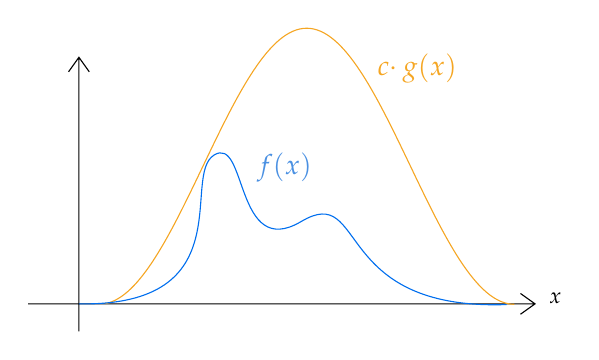
\begin{tikzpicture}[x=0.75pt,y=0.75pt,yscale=-1,xscale=1]
%uncomment if require: \path (0,195); %set diagram left start at 0, and has height of 195

%Shape: Axis 2D [id:dp04454782868493701] 
\draw  (48,169.8) -- (292.17,169.8)(72.42,51) -- (72.42,183) (285.17,164.8) -- (292.17,169.8) -- (285.17,174.8) (67.42,58) -- (72.42,51) -- (77.42,58)  ;
%Shape: Wave [id:dp3551881077157548] 
\draw  [color={rgb, 255:red, 245; green, 166; blue, 35 }  ,draw opacity=1 ] (282.17,170) .. controls (264.07,170) and (248.47,137.57) .. (232.17,103.5) .. controls (215.86,69.43) and (200.26,37) .. (182.17,37) .. controls (164.07,37) and (148.47,69.43) .. (132.17,103.5) .. controls (116.77,135.67) and (102,166.38) .. (85.17,169.7) ;
%Curve Lines [id:da9058629039644694] 
\draw [color={rgb, 255:red, 0; green, 110; blue, 238 }  ,draw opacity=1 ]   (72.42,169.8) .. controls (151.5,171.13) and (121.5,108.13) .. (137.5,98.13) .. controls (153.5,88.13) and (147.5,149.13) .. (179.5,130.13) .. controls (211.5,111.13) and (193.5,173.13) .. (278.5,170.13) ;

% Text Node
\draw (302,167) node  [font=\footnotesize] [align=left] {$\displaystyle x$};
% Text Node
\draw (215,48) node [anchor=north west][inner sep=0.75pt]  [color={rgb, 255:red, 245; green, 166; blue, 35 }  ,opacity=1 ] [align=left] {$\displaystyle c\cdotp g( x)$};
% Text Node
\draw (157,96) node [anchor=north west][inner sep=0.75pt]  [color={rgb, 255:red, 74; green, 144; blue, 226 }  ,opacity=1 ] [align=left] {$\displaystyle f( x)$};
\end{tikzpicture}
		\end{center}
	\item	Simuler une réalisation $y_{j}$ de la variable aléatoire $Y$ ayant la fonction de densité $g$ et calculer $\frac{f(y_{j})}{c g(y_{j})}$.	
	\item	Simuler une réalisation $u_{j}$ de la variable aléatoire $U(0, 1)$.
	\item	Comparer la réalisation $u_{j}$ à $\frac{f(y_{j})}{c g(y_{j})}$, si \lfbox[formula]{$u_{j} \leq \frac{f(y_{j})}{c g(y_{j})}$} alors accepter la réalisation $y_{j}$, sinon la refuser et retourner à l'étape 2.
	\begin{center}
\tikzset{every picture/.style={line width=0.75pt}} %set default line width to 0.75pt        
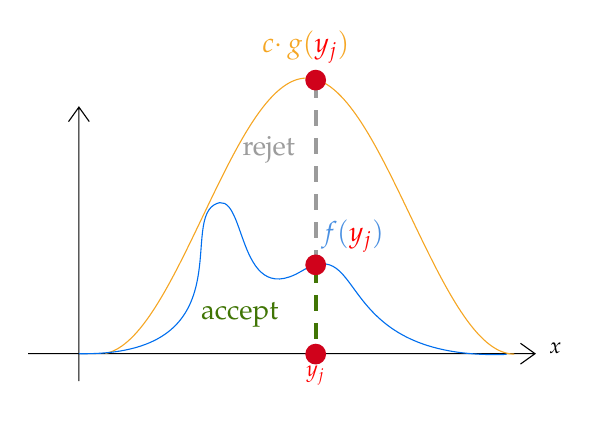
\begin{tikzpicture}[x=0.75pt,y=0.75pt,yscale=-1,xscale=1]
%uncomment if require: \path (0,247); %set diagram left start at 0, and has height of 247

%Shape: Axis 2D [id:dp9159544224440075] 
\draw  (48,169.8) -- (292.17,169.8)(72.42,51) -- (72.42,183) (285.17,164.8) -- (292.17,169.8) -- (285.17,174.8) (67.42,58) -- (72.42,51) -- (77.42,58)  ;
%Shape: Wave [id:dp7772804532155415] 
\draw  [color={rgb, 255:red, 245; green, 166; blue, 35 }  ,draw opacity=1 ] (282.17,170) .. controls (264.07,170) and (248.47,137.57) .. (232.17,103.5) .. controls (215.86,69.43) and (200.26,37) .. (182.17,37) .. controls (164.07,37) and (148.47,69.43) .. (132.17,103.5) .. controls (116.77,135.67) and (102,166.38) .. (85.17,169.7) ;
%Curve Lines [id:da5198385313052689] 
\draw [color={rgb, 255:red, 0; green, 110; blue, 238 }  ,draw opacity=1 ]   (72.42,169.8) .. controls (151.5,171.13) and (121.5,108.13) .. (137.5,98.13) .. controls (153.5,88.13) and (147.5,149.13) .. (179.5,130.13) .. controls (211.5,111.13) and (193.5,173.13) .. (278.5,170.13) ;
%Straight Lines [id:da15724953888704207] 
\draw [color={rgb, 255:red, 155; green, 155; blue, 155 }  ,draw opacity=1 ][line width=1.5]  [dash pattern={on 5.63pt off 4.5pt}]  (186.5,39) -- (186.5,128) ;
%Straight Lines [id:da2978344643989861] 
\draw [color={rgb, 255:red, 65; green, 117; blue, 5 }  ,draw opacity=1 ][line width=1.5]  [dash pattern={on 5.63pt off 4.5pt}]  (186.5,128) -- (186.5,171) ;
%Shape: Circle [id:dp23396862805085927] 
\draw  [draw opacity=0][fill={rgb, 255:red, 208; green, 2; blue, 27 }  ,fill opacity=1 ] (181.5,38) .. controls (181.5,35.24) and (183.74,33) .. (186.5,33) .. controls (189.26,33) and (191.5,35.24) .. (191.5,38) .. controls (191.5,40.76) and (189.26,43) .. (186.5,43) .. controls (183.74,43) and (181.5,40.76) .. (181.5,38) -- cycle ;
%Shape: Circle [id:dp056157791101330234] 
\draw  [draw opacity=0][fill={rgb, 255:red, 208; green, 2; blue, 27 }  ,fill opacity=1 ] (181.5,127) .. controls (181.5,124.24) and (183.74,122) .. (186.5,122) .. controls (189.26,122) and (191.5,124.24) .. (191.5,127) .. controls (191.5,129.76) and (189.26,132) .. (186.5,132) .. controls (183.74,132) and (181.5,129.76) .. (181.5,127) -- cycle ;
%Shape: Circle [id:dp7790187571587763] 
\draw  [draw opacity=0][fill={rgb, 255:red, 208; green, 2; blue, 27 }  ,fill opacity=1 ] (181.5,170) .. controls (181.5,167.24) and (183.74,165) .. (186.5,165) .. controls (189.26,165) and (191.5,167.24) .. (191.5,170) .. controls (191.5,172.76) and (189.26,175) .. (186.5,175) .. controls (183.74,175) and (181.5,172.76) .. (181.5,170) -- cycle ;

% Text Node
\draw (302,167) node  [font=\footnotesize] [align=left] {$\displaystyle x$};
% Text Node
\draw (159.5,13) node [anchor=north west][inner sep=0.75pt]  [color={rgb, 255:red, 245; green, 166; blue, 35 }, opacity=1 ] [align=left] {$\displaystyle c\cdotp g(\textcolor[rgb]{1, 0, 0}{y_{j}}\textcolor[rgb]{0.96, 0.65, 0.14}{)}$};
% Text Node
\draw (188,104) node [anchor=north west][inner sep=0.75pt]  [color={rgb, 255:red, 74; green, 144; blue, 226 }  ,opacity=1 ] [align=left] {$\displaystyle f(\textcolor[rgb]{1, 0, 0}{y_{j}}\textcolor[rgb]{0.29, 0.56, 0.88}{)}$};
% Text Node
\draw (186.5,180.33) node  [font=\footnotesize] [align=left] {$\displaystyle \textcolor[rgb]{1, 0, 0}{y_{j}}$};
% Text Node
\draw (130,144) node [anchor=north west][inner sep=0.75pt]   [align=left] {\textcolor[rgb]{0.25,0.46,0.02}{accept}};
% Text Node
\draw (150,64) node [anchor=north west][inner sep=0.75pt]   [align=left] {\textcolor[rgb]{0.61,0.61,0.61}{rejet}};
\end{tikzpicture}
	\end{center}
\end{enumerate}

Les nombres simulés vont suivre la distribution associée à la fonction de densité $f$.
\paragraph{Note}	Le nombre d'itérations nécessaires pour obtenir un nombre aléatoire simulé suit une distribution géométrique de moyenne $c$.
\end{algo2}


\subsection{Simulation Monte-Carlo}
\begin{algo2}[Simulation Monte-Carlo]
Pour une variable aléatoire $X$, 
\begin{enumerate}[label = \circled{\arabic*}{trueblue}]
	\item	Simuler un vecteur de réalisation $(x_{1}, x_{2}, \dots, x_{n})$ d'une distribution dont la fonction de densité est $f(x_{1}, x_{2}, \dots, x_{n})$.
	\item	Appliquer une fonction $g$ au vecteur des réalisations pour trouver $y_{j} = g(x_{1}, x_{2}, \dots, x_{n})$.
	\item	Répéter les étapes 1 et 2 $r$ fois où $r$ est grand.
	\item	Calculer la valeur désiré (espérance, variance, etc.) avec les réalisations $(y_{1}, y_{2}, \dots, y_{r})$.
\end{enumerate}
\end{algo2}

Visuellement : 
\begin{center}
\tikzset{every picture/.style={line width=0.75pt}} %set default line width to 0.75pt        
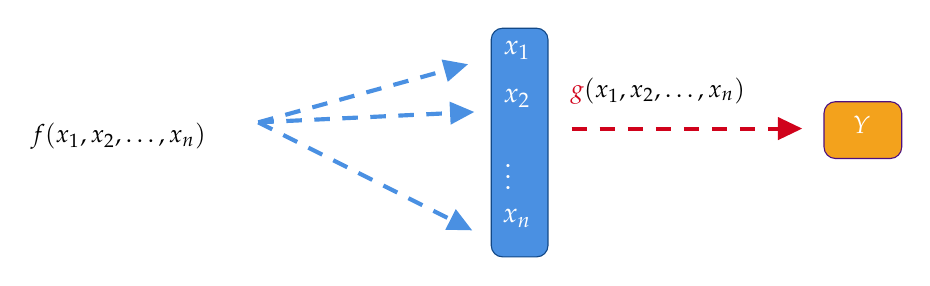
\begin{tikzpicture}[x=0.75pt,y=0.75pt,yscale=-1,xscale=1]
%uncomment if require: \path (0,168); %set diagram left start at 0, and has height of 168


%Rounded Rect [id:dp942454310600852] 
\draw  [color={rgb, 255:red, 18; green, 72; blue, 135 }  ,draw opacity=1 ][fill={rgb, 255:red, 74; green, 144; blue, 226 }  ,fill opacity=1 ] (253.61,34.92) .. controls (256.63,34.92) and (259.08,37.36) .. (259.08,40.38) -- (259.08,139.62) .. controls (259.08,142.64) and (256.63,145.08) .. (253.61,145.08) -- (237.21,145.08) .. controls (234.19,145.08) and (231.74,142.64) .. (231.74,139.62) -- (231.74,40.38) .. controls (231.74,37.36) and (234.19,34.92) .. (237.21,34.92) -- cycle ;

%Rounded Rect [id:dp12379698936527883] 
\draw  [color={rgb, 255:red, 76; green, 16; blue, 128 }  ,draw opacity=1 ][fill={rgb, 255:red, 243; green, 162; blue, 28 }  ,fill opacity=1 ] (392.08,75.8) .. controls (392.08,72.78) and (394.53,70.33) .. (397.55,70.33) -- (424.03,70.33) .. controls (427.05,70.33) and (429.5,72.78) .. (429.5,75.8) -- (429.5,92.2) .. controls (429.5,95.22) and (427.05,97.67) .. (424.03,97.67) -- (397.55,97.67) .. controls (394.53,97.67) and (392.08,95.22) .. (392.08,92.2) -- cycle ;

%Straight Lines [id:da8321642773139506] 
\draw [color={rgb, 255:red, 74; green, 144; blue, 226 }  ,draw opacity=1 ][line width=1.5]  [dash pattern={on 5.63pt off 4.5pt}]  (119.5,80.27) -- (216.65,53.34) ;
\draw [shift={(220.5,52.27)}, rotate = 524.51] [fill={rgb, 255:red, 74; green, 144; blue, 226 }  ,fill opacity=1 ][line width=0.08]  [draw opacity=0] (11.61,-5.58) -- (0,0) -- (11.61,5.58) -- cycle    ;
%Straight Lines [id:da4555457784342194] 
\draw [color={rgb, 255:red, 74; green, 144; blue, 226 }  ,draw opacity=1 ][line width=1.5]  [dash pattern={on 5.63pt off 4.5pt}]  (119.5,80.27) -- (219.5,75.47) ;
\draw [shift={(223.5,75.27)}, rotate = 537.25] [fill={rgb, 255:red, 74; green, 144; blue, 226 }  ,fill opacity=1 ][line width=0.08]  [draw opacity=0] (11.61,-5.58) -- (0,0) -- (11.61,5.58) -- cycle    ;
%Straight Lines [id:da5524460861328313] 
\draw [color={rgb, 255:red, 74; green, 144; blue, 226 }  ,draw opacity=1 ][line width=1.5]  [dash pattern={on 5.63pt off 4.5pt}]  (119.5,80.27) -- (218.93,130.47) ;
\draw [shift={(222.5,132.27)}, rotate = 206.79] [fill={rgb, 255:red, 74; green, 144; blue, 226 }  ,fill opacity=1 ][line width=0.08]  [draw opacity=0] (11.61,-5.58) -- (0,0) -- (11.61,5.58) -- cycle    ;
%Straight Lines [id:da19756141741178124] 
\draw [color={rgb, 255:red, 208; green, 2; blue, 27 }  ,draw opacity=1 ][line width=1.5]  [dash pattern={on 5.63pt off 4.5pt}]  (270.5,83.27) -- (377.5,83.27) ;
\draw [shift={(381.5,83.27)}, rotate = 180] [fill={rgb, 255:red, 208; green, 2; blue, 27 }  ,fill opacity=1 ][line width=0.08]  [draw opacity=0] (11.61,-5.58) -- (0,0) -- (11.61,5.58) -- cycle    ;

% Text Node
\draw (236.41,40) node [anchor=north west][inner sep=0.75pt]  [color={rgb, 255:red, 255; green, 255; blue, 255 }  ,opacity=1 ] [align=left] {$\displaystyle x_{1}$};
% Text Node
\draw (236.41,63) node [anchor=north west][inner sep=0.75pt]  [color={rgb, 255:red, 255; green, 255; blue, 255 }  ,opacity=1 ] [align=left] {$\displaystyle x_{2}$};
% Text Node
\draw (235.91,121) node [anchor=north west][inner sep=0.75pt]  [color={rgb, 255:red, 255; green, 255; blue, 255 }  ,opacity=1 ] [align=left] {$\displaystyle x_{n}$};
% Text Node
\draw (236.91,91) node [anchor=north west][inner sep=0.75pt]  [color={rgb, 255:red, 255; green, 255; blue, 255 }  ,opacity=1 ] [align=left] {$\displaystyle \vdots $};
% Text Node
\draw (8.66,79.5) node [anchor=north west][inner sep=0.75pt]  [font=\small,color={rgb, 255:red, 0; green, 0; blue, 0 }  ,opacity=1 ] [align=left] {$\displaystyle f( x_{1} ,x_{2} ,\dotsc ,x_{n})$};
% Text Node
\draw (268.66,57.5) node [anchor=north west][inner sep=0.75pt]  [font=\small,color={rgb, 255:red, 0; green, 0; blue, 0 }  ,opacity=1 ] [align=left] {$\displaystyle \textcolor[rgb]{0.82,0.01,0.11}{g}( x_{1} ,x_{2} ,\dotsc ,x_{n})$};
% Text Node
\draw (404.79,76) node [anchor=north west][inner sep=0.75pt]  [font=\small,color={rgb, 255:red, 255; green, 255; blue, 255 }  ,opacity=1 ] [align=left] {$\displaystyle Y$};
\end{tikzpicture}
\end{center}





\newpage
\part{Processus stochastiques}
\label{chapt:procStoch}
\section{Introduction}
\begin{distributions}[Notation]
\begin{description}
	\item[$X_{n}$]	État du processus au temps $n$.
		\begin{itemize}
		\item	Par exemple, si $X_{n}	=	i$ alors le processus est dit d'être dans l'état $i$ au temps $n$.
		\end{itemize}
\end{description}
\end{distributions}

\begin{definitionNOHFILL}[Processus stochastique]
Soit le processus stochastique \lfbox[formula]{$\{X_{n}, n	=	0, 1, 2, \dots\}$}.
\end{definitionNOHFILL}


\columnbreak
\section{Processus de Poisson}
\label{sec:procPois}
\begin{distributions}[Notation]
\begin{description}
	\item[$\lambda(t)$]	Fonction d'intensité d'un processus de Poisson.
		\begin{itemize}
		\item	En anglais, \og \textit{rate function} \fg{}.
		\end{itemize}
\end{description}
\end{distributions}
\begin{definitionNOHFILL}[Processus stochastique]
Une collection de variables aléatoires.
\end{definitionNOHFILL}

\begin{definitionNOHFILLsub}[Processus de comptage]
On dénote le processus de comptage par \lfbox[formula]{$\underline{N}	=	\{N(t), t \geq 0\}$}. Le processus \textbf{compte le nombre d'événements} qui se produisent dans l'intervalle de temps $(0, t]$ où \lfbox[conditions]{$t > 0$}.\\

En termes mathématiques, c'est un processus stochastique dont les variables aléatoires prennent des valeurs non décroissantes et non négatives sous les conditions suivantes :
\begin{enumerate}
	\item	$N(0) = 0$ ;
	\item	$N(t) \geq 0$ \textit{(valeurs non négatives)};
	\item	$N(t)$ est entier ;
	\item	$N(t + h) \geq N(h)$ pour $h	>	0$ \textit{(valeurs non décroissantes)}.
\end{enumerate}

\

Visuellement, on voir que l'\textbf{accroissement} $N(t + h) - N(t)$ représente le nombre d'événements produits sur l'intervalle $(t, t + h]$ :
\begin{center}
\tikzset{every picture/.style={line width=0.75pt}} %set default line width to 0.75pt        
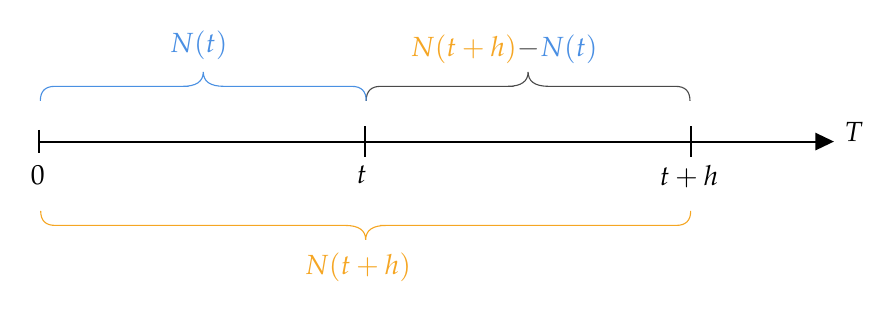
\begin{tikzpicture}[x=0.75pt,y=0.75pt,yscale=-1,xscale=1]
%uncomment if require: \path (0,163); %set diagram left start at 0, and has height of 163

%Straight Lines [id:da8473597783790416] 
\draw [color={rgb, 255:red, 0; green, 0; blue, 0 }  ,draw opacity=1 ][line width=0.75]    (82.36,63.61) -- (462.17,63.61) (239.36,56.11) -- (239.36,71.11)(396.36,56.11) -- (396.36,71.11) ;
\draw [shift={(465.17,63.61)}, rotate = 180] [fill={rgb, 255:red, 0; green, 0; blue, 0 }  ,fill opacity=1 ][line width=0.08]  [draw opacity=0] (8.93,-4.29) -- (0,0) -- (8.93,4.29) -- cycle    ;
\draw [shift={(82.36,63.61)}, rotate = 180] [color={rgb, 255:red, 0; green, 0; blue, 0 }  ,draw opacity=1 ][line width=0.75]    (0,5.59) -- (0,-5.59)   ;
%Shape: Brace [id:dp9118751878351816] 
\draw  [color={rgb, 255:red, 245; green, 166; blue, 35 }  ,draw opacity=1 ] (83,97) .. controls (83,101.67) and (85.33,104) .. (90,104) -- (229.58,104) .. controls (236.25,104) and (239.58,106.33) .. (239.58,111) .. controls (239.58,106.33) and (242.91,104) .. (249.58,104)(246.58,104) -- (389.17,104) .. controls (393.84,104) and (396.17,101.67) .. (396.17,97) ;
%Shape: Brace [id:dp6636434796853381] 
\draw  [color={rgb, 255:red, 74; green, 74; blue, 74 }  ,draw opacity=1 ] (395.83,44) .. controls (395.83,39.33) and (393.5,37) .. (388.83,37) -- (327.83,37) .. controls (321.16,37) and (317.83,34.67) .. (317.83,30) .. controls (317.83,34.67) and (314.5,37) .. (307.83,37)(310.83,37) -- (246.83,37) .. controls (242.16,37) and (239.83,39.33) .. (239.83,44) ;
%Shape: Brace [id:dp2842213365224564] 
\draw  [color={rgb, 255:red, 74; green, 144; blue, 226 }  ,draw opacity=1 ] (239.83,44) .. controls (239.83,39.33) and (237.5,37) .. (232.83,37) -- (171.33,37) .. controls (164.66,37) and (161.33,34.67) .. (161.33,30) .. controls (161.33,34.67) and (158,37) .. (151.33,37)(154.33,37) -- (89.83,37) .. controls (85.16,37) and (82.83,39.33) .. (82.83,44) ;

% Text Node
\draw (234,74) node [anchor=north west][inner sep=0.75pt]   [align=left] {$\displaystyle t$};
% Text Node
\draw (380,74) node [anchor=north west][inner sep=0.75pt]   [align=left] {$\displaystyle t+h$};
% Text Node
\draw (469,53) node [anchor=north west][inner sep=0.75pt]   [align=left] {$\displaystyle T$};
% Text Node
\draw (77,74) node [anchor=north west][inner sep=0.75pt]   [align=left] {$\displaystyle 0$};
% Text Node
\draw (209,116) node [anchor=north west][inner sep=0.75pt]   [align=left] {$\displaystyle \textcolor[rgb]{0.96,0.65,0.14}{N( t+h)}$};
% Text Node
\draw (260,11) node [anchor=north west][inner sep=0.75pt]   [align=left] {$\displaystyle \textcolor[rgb]{0.96,0.65,0.14}{N}\textcolor[rgb]{0.96,0.65,0.14}{(}\textcolor[rgb]{0.96,0.65,0.14}{t+h}\textcolor[rgb]{0.96,0.65,0.14}{)}\textcolor[rgb]{0.29,0.29,0.29}{-}\textcolor[rgb]{0.29,0.56,0.89}{N( t)}$};
% Text Node
\draw (144,9) node [anchor=north west][inner sep=0.75pt]   [align=left] {$\displaystyle \textcolor[rgb]{0.29,0.56,0.89}{N( t)}$};
\end{tikzpicture}
\end{center}

\tcbline

\begin{itemize}
	\item	Alias, processus de dénombrement.
\end{itemize}
\end{definitionNOHFILLsub}

\begin{definitionNOHFILLsub}[Processus de Poisson]
Processus de comptage dont :
\begin{enumerate}
	\item	chaque accroissement est une variable aléatoire de Poisson,
	\item	les accroissements qui ne se \textbf{chevauchent pas} sont indépendants.
\end{enumerate}

\

Pour un processus de Poisson avec \textbf{fonction d'intensité} $\lambda(t)$, l'accroissement \lfbox[formula]{$N(t + h) - N(t)	\sim	\text{Poisson}\left(\lambda	=	\int_{t}^{t + h}\lambda(u)du\right)$}. 
\begin{itemize}
	\item	On pose donc que le paramètre de la fréquence des accroissements $\lambda$ est la \textit{moyenne} de la fonction d'intensité des accroissements $\lambda(t)$ sur l'intervalle de temps $(t, t + h]$.
\end{itemize}

\begin{definitionNOHFILLprop}[Processus de Poisson homogène]
Si la fonction d'intensité est constante, \lfbox[conditions]{$\lambda(t)	=	\lambda$}, le processus $\underline{N}$ est un \textbf{processus de Poisson homogène} et \lfbox[formula]{$N(t + h)	-	N(t)	\sim	\text{Poisson}(\lambda t)$}.
\end{definitionNOHFILLprop}

\begin{definitionNOHFILLprop}[Processus de Poisson non homogène]
Si la fonction d'intensité varie avec le temps $t$, le processus $\underline{N}$ est un \textbf{processus de Poisson non homogène}.
\end{definitionNOHFILLprop}
\end{definitionNOHFILLsub}


\columnbreak
\subsection{Temps d'occurrence}
\begin{distributions}[Notation]
\begin{description}
	\item[$T_{k}$]	Temps d'occurrence du $k^{e}$ événement.
		\begin{itemize}
		\item	\lfbox[formula]{$T_{k}	=	V_{1} + V_{2} + \dots + V_{k}$}.
		\end{itemize}
	\item[$V_{k}$]	Intervalle de temps entre la réalisation du $(k - 1)^{e}$ et du $k^{e}$ événement.
		\begin{itemize}
		\item	Alias, le temps inter arrivé.
		\item	\lfbox[formula]{$V_{k}	=	T_{k} - T_{k - 1}$}.
		\item	On pose que \lfbox[conditions]{$T_{0} = 0$}, \lfbox[conditions]{$V_{0} = 0$} et que \lfbox[conditions]{$V_{1}	=	T_{1}$}.
		\end{itemize}
\end{description}
\end{distributions}

Visuellement : 
\begin{center}
\tikzset{every picture/.style={line width=0.75pt}} %set default line width to 0.75pt        
\begin{tikzpicture}[x=0.75pt,y=0.75pt,yscale=-1,xscale=1]
%uncomment if require: \path (0,218); %set diagram left start at 0, and has height of 218

%Straight Lines [id:da8473597783790416] 
\draw [color={rgb, 255:red, 0; green, 0; blue, 0 }  ,draw opacity=1 ][line width=0.75]    (82.36,83.61) -- (462.17,83.61) (204.36,76.11) -- (204.36,91.11)(326.36,76.11) -- (326.36,91.11)(448.36,76.11) -- (448.36,91.11) ;
\draw [shift={(465.17,83.61)}, rotate = 180] [fill={rgb, 255:red, 0; green, 0; blue, 0 }  ,fill opacity=1 ][line width=0.08]  [draw opacity=0] (8.93,-4.29) -- (0,0) -- (8.93,4.29) -- cycle    ;
\draw [shift={(82.36,83.61)}, rotate = 180] [color={rgb, 255:red, 0; green, 0; blue, 0 }  ,draw opacity=1 ][line width=0.75]    (0,5.59) -- (0,-5.59)   ;
%Shape: Brace [id:dp9118751878351816] 
\draw  [color={rgb, 255:red, 44; green, 109; blue, 184 }  ,draw opacity=1 ] (83,117) .. controls (83,121.67) and (85.33,124) .. (90,124) -- (133.75,124) .. controls (140.42,124) and (143.75,126.33) .. (143.75,131) .. controls (143.75,126.33) and (147.08,124) .. (153.75,124)(150.75,124) -- (197.5,124) .. controls (202.17,124) and (204.5,121.67) .. (204.5,117) ;
%Rounded Rect [id:dp11465036181300836] 
\draw  [color={rgb, 255:red, 18; green, 72; blue, 135 }  ,draw opacity=1 ][fill={rgb, 255:red, 74; green, 144; blue, 226 }  ,fill opacity=1 ] (188,43) .. controls (188,39.41) and (190.91,36.5) .. (194.5,36.5) -- (214,36.5) .. controls (217.59,36.5) and (220.5,39.41) .. (220.5,43) -- (220.5,65) .. controls (220.5,68.59) and (217.59,71.5) .. (214,71.5) -- (194.5,71.5) .. controls (190.91,71.5) and (188,68.59) .. (188,65) -- cycle ;

%Rounded Rect [id:dp5256044584805744] 
\draw  [color={rgb, 255:red, 99; green, 64; blue, 6 }  ,draw opacity=1 ][fill={rgb, 255:red, 245; green, 164; blue, 29 }  ,fill opacity=1 ] (309,43) .. controls (309,39.41) and (311.91,36.5) .. (315.5,36.5) -- (335,36.5) .. controls (338.59,36.5) and (341.5,39.41) .. (341.5,43) -- (341.5,65) .. controls (341.5,68.59) and (338.59,71.5) .. (335,71.5) -- (315.5,71.5) .. controls (311.91,71.5) and (309,68.59) .. (309,65) -- cycle ;
%Rounded Rect [id:dp08392234396619447] 
\draw  [color={rgb, 255:red, 39; green, 70; blue, 3 }  ,draw opacity=1 ][fill={rgb, 255:red, 126; green, 211; blue, 33 }  ,fill opacity=1 ] (431,43) .. controls (431,39.41) and (433.91,36.5) .. (437.5,36.5) -- (457,36.5) .. controls (460.59,36.5) and (463.5,39.41) .. (463.5,43) -- (463.5,65) .. controls (463.5,68.59) and (460.59,71.5) .. (457,71.5) -- (437.5,71.5) .. controls (433.91,71.5) and (431,68.59) .. (431,65) -- cycle ;
%Shape: Brace [id:dp26377470569710515] 
\draw  [color={rgb, 255:red, 245; green, 166; blue, 35 }  ,draw opacity=1 ] (205,117) .. controls (205,121.67) and (207.33,124) .. (212,124) -- (255.75,124) .. controls (262.42,124) and (265.75,126.33) .. (265.75,131) .. controls (265.75,126.33) and (269.08,124) .. (275.75,124)(272.75,124) -- (319.5,124) .. controls (324.17,124) and (326.5,121.67) .. (326.5,117) ;
%Shape: Brace [id:dp2470075020847542] 
\draw  [color={rgb, 255:red, 120; green, 201; blue, 32 }  ,draw opacity=1 ] (327,117) .. controls (327,121.67) and (329.33,124) .. (334,124) -- (377.75,124) .. controls (384.42,124) and (387.75,126.33) .. (387.75,131) .. controls (387.75,126.33) and (391.08,124) .. (397.75,124)(394.75,124) -- (441.5,124) .. controls (446.17,124) and (448.5,121.67) .. (448.5,117) ;
%Shape: Brace [id:dp44214970032790535] 
\draw  [color={rgb, 255:red, 208; green, 2; blue, 27 }  ,draw opacity=1 ] (83,152) .. controls (83,156.67) and (85.33,159) .. (90,159) -- (255.75,159) .. controls (262.42,159) and (265.75,161.33) .. (265.75,166) .. controls (265.75,161.33) and (269.08,159) .. (275.75,159)(272.75,159) -- (441.5,159) .. controls (446.17,159) and (448.5,156.67) .. (448.5,152) ;

% Text Node
\draw (200,92) node [anchor=north west][inner sep=0.75pt]   [align=left] {$\displaystyle t_{1}$};
% Text Node
\draw (469,73) node [anchor=north west][inner sep=0.75pt]   [align=left] {$\displaystyle T$};
% Text Node
\draw (77,94) node [anchor=north west][inner sep=0.75pt]   [align=left] {$\displaystyle 0$};
% Text Node
\draw (198.75,45) node [anchor=north west][inner sep=0.75pt]  [color={rgb, 255:red, 255; green, 255; blue, 255 }  ,opacity=1 ] [align=left] {\textcolor[rgb]{1,1,1}{$\displaystyle 1$}};
% Text Node
\draw (319.75,45) node [anchor=north west][inner sep=0.75pt]  [color={rgb, 255:red, 255; green, 255; blue, 255 }  ,opacity=1 ] [align=left] {\textcolor[rgb]{1,1,1}{$\displaystyle 2$}};
% Text Node
\draw (441.75,45) node [anchor=north west][inner sep=0.75pt]  [color={rgb, 255:red, 255; green, 255; blue, 255 }  ,opacity=1 ] [align=left] {\textcolor[rgb]{1,1,1}{$\displaystyle 3$}};
% Text Node
\draw (323,92) node [anchor=north west][inner sep=0.75pt]   [align=left] {$\displaystyle t_{2}$};
% Text Node
\draw (444,92) node [anchor=north west][inner sep=0.75pt]   [align=left] {$\displaystyle t_{3}$};
% Text Node
\draw (136,132) node [anchor=north west][inner sep=0.75pt]   [align=left] {$\displaystyle \textcolor[rgb]{0.29,0.56,0.89}{V_{1}}$};
% Text Node
\draw (258,132) node [anchor=north west][inner sep=0.75pt]   [align=left] {$\displaystyle \textcolor[rgb]{0.96,0.65,0.14}{V_{2}}$};
% Text Node
\draw (378,132) node [anchor=north west][inner sep=0.75pt]   [align=left] {$\displaystyle \textcolor[rgb]{0.45,0.76,0.11}{V_{3}}$};
% Text Node
\draw (197,172) node [anchor=north west][inner sep=0.75pt]   [align=left] {$\displaystyle \textcolor[rgb]{0.82,0.01,0.11}{T_{3} =}\textcolor[rgb]{0.29,0.56,0.89}{V}\textcolor[rgb]{0.29,0.56,0.89}{_{1}}\textcolor[rgb]{0.29,0.29,0.29}{+}\textcolor[rgb]{0.96,0.65,0.14}{V}\textcolor[rgb]{0.96,0.65,0.14}{_{2}}\textcolor[rgb]{0.29,0.29,0.29}{+}\textcolor[rgb]{0.45,0.76,0.11}{V}\textcolor[rgb]{0.45,0.76,0.11}{_{3}}$};
\end{tikzpicture}
\end{center}

\begin{definitionNOHFILL}[Temps d'occurrence]
On peut définir le processus de comptage en fonction du temps d'occurrence des événements au lieu nombre de sinistres : \lfbox[formula]{$N(t)	=	\sup\{k \geq 1 : T_{k} \leq t\}$}, \lfbox[conditions]{$\forall t \geq 0$}. 

On trouve que \lfbox[formula]{$\Pr(T_{k} > s)	=	\Pr(N(s) < k)$}. C'est-à-dire, $\Pr\left(\substack{\text{le $k^{e}$ événement se produise}\\ \text{après le temps $s$}}\right)	=	\Pr\left(\substack{\text{moins de $k$ événements se}\\ \text{produisent d'ici le temps $s$}}\right)$.
\end{definitionNOHFILL}

\begin{definitionNOHFILLprop}[Temps d'occurrence pour des processus de Poisson homogènes]
Si \lfbox[conditions]{$N(t) \sim \text{Poisson}(\lambda t)$} alors \lfbox[formula]{$V_{k} \sim \text{Exp}\left(\theta	=	\frac{1}{\lambda}\right)$} et \lfbox[formula]{$T_{k} \sim \text{Gamma}\left(\alpha = k, \theta	=	\frac{1}{\lambda}\right) \sim \text{Erlang}\left(n = k, \lambda\right)$}.\\

\paragraph{Note}	La loi Gamma avec un paramètre de forme $\alpha$ entier correspond à la loi Erlang. L'avantage de la loi Erlang est qu'elle a une fonction de répartition explicite qui découle de la relation entre les processus de Poisson et les temps d'occurrences. Voir la sous-section sur les \textbf{\nameref{subsec:distrIARD}} du chapitre de \nameref{chapt:mathIARD}.
\end{definitionNOHFILLprop}


\subsubsection{Temps d'occurrence conditionnels}
\paragraph{Note}	Voir la sous-section des \textbf{\nameref{subsec:orderStats}} du chapitre de \nameref{chapt:stats}.

\

Lorsque nous savons qu'un certain nombre d'événements se produit d'ici un temps $t$, les temps d'occurrences $T_{1}, T_{2}, \dots, T_{n}$ ne \textbf{suivent plus une distribution Gamma}. Ceci est puisque \textbf{leurs domaines sont \textit{bornés} à $t$} au lieu d'être \textit{\textbf{infinis}}. \\

Par exemple, $N(t) = n$ implique que $T_{1}, T_{2}, \dots, T_{n} \leq t$ :
\begin{center}
\tikzset{every picture/.style={line width=0.75pt}} %set default line width to 0.75pt        
\begin{tikzpicture}[x=0.75pt,y=0.75pt,yscale=-1,xscale=1]
%uncomment if require: \path (0,163); %set diagram left start at 0, and has height of 163

%Straight Lines [id:da7067911474403936] 
\draw [color={rgb, 255:red, 0; green, 0; blue, 0 }  ,draw opacity=1 ][line width=0.75]    (82.36,63.61) -- (396.17,63.61) (239.36,56.11) -- (239.36,71.11) ;
\draw [shift={(399.17,63.61)}, rotate = 180] [fill={rgb, 255:red, 0; green, 0; blue, 0 }  ,fill opacity=1 ][line width=0.08]  [draw opacity=0] (8.93,-4.29) -- (0,0) -- (8.93,4.29) -- cycle    ;
\draw [shift={(82.36,63.61)}, rotate = 180] [color={rgb, 255:red, 0; green, 0; blue, 0 }  ,draw opacity=1 ][line width=0.75]    (0,5.59) -- (0,-5.59)   ;
%Shape: Brace [id:dp44073656005149386] 
\draw  [color={rgb, 255:red, 74; green, 144; blue, 226 }  ,draw opacity=1 ] (239.83,44) .. controls (239.83,39.33) and (237.5,37) .. (232.83,37) -- (171.33,37) .. controls (164.66,37) and (161.33,34.67) .. (161.33,30) .. controls (161.33,34.67) and (158,37) .. (151.33,37)(154.33,37) -- (89.83,37) .. controls (85.16,37) and (82.83,39.33) .. (82.83,44) ;
%Straight Lines [id:da4478875067752026] 
\draw [color={rgb, 255:red, 111; green, 18; blue, 193 }  ,draw opacity=1 ][line width=1.5]    (82.36,63.61) -- (240.17,63.61) (239.36,56.11) -- (239.36,71.11) ;
\draw [shift={(82.36,63.61)}, rotate = 180] [color={rgb, 255:red, 111; green, 18; blue, 193 }  ,draw opacity=1 ][line width=1.5]    (0,6.71) -- (0,-6.71)   ;
%Rounded Rect [id:dp29009509835708336] 
\draw  [color={rgb, 255:red, 18; green, 72; blue, 135 }  ,draw opacity=1 ][fill={rgb, 255:red, 111; green, 18; blue, 193 }  ,fill opacity=1 ] (126,108.5) .. controls (126,104.63) and (129.13,101.5) .. (133,101.5) -- (335.17,101.5) .. controls (339.03,101.5) and (342.17,104.63) .. (342.17,108.5) -- (342.17,129.5) .. controls (342.17,133.37) and (339.03,136.5) .. (335.17,136.5) -- (133,136.5) .. controls (129.13,136.5) and (126,133.37) .. (126,129.5) -- cycle ;
%Shape: Triangle [id:dp8326527885637682] 
\draw  [draw opacity=0][fill={rgb, 255:red, 144; green, 19; blue, 254 }  ,fill opacity=1 ] (238.67,90.75) -- (248.17,101.61) -- (229.17,101.61) -- cycle ;

% Text Node
\draw (235,74) node [anchor=north west][inner sep=0.75pt]   [align=left] {$\displaystyle t$};
% Text Node
\draw (402,52) node [anchor=north west][inner sep=0.75pt]   [align=left] {$\displaystyle T$};
% Text Node
\draw (77,74) node [anchor=north west][inner sep=0.75pt]   [align=left] {$\displaystyle 0$};
% Text Node
\draw (131,10) node [anchor=north west][inner sep=0.75pt]   [align=left] {$\displaystyle \textcolor[rgb]{0.29,0.56,0.89}{N}\textcolor[rgb]{0.29,0.56,0.89}{(}\textcolor[rgb]{0.29,0.56,0.89}{t}\textcolor[rgb]{0.29,0.56,0.89}{) =n}$};
% Text Node
\draw (152.58,110) node [anchor=north west][inner sep=0.75pt]  [color={rgb, 255:red, 255; green, 255; blue, 255 }  ,opacity=1 ] [align=left] {\textcolor[rgb]{1,1,1}{$\displaystyle ( T_{1} ,T_{2} ,\dotsc ,T_{n} |N( t) =n) \leq t$}};
\end{tikzpicture}
\end{center}

\

On en déduit que les temps d'occurrences sont en fait des \textbf{\nameref{subsec:orderStats}} avec $0 < T_{1} \leq T_{2} \leq \dots \leq T_{n} \leq t$ : 
\begin{center}
\tikzset{every picture/.style={line width=0.75pt}} %set default line width to 0.75pt        
\begin{tikzpicture}[x=0.75pt,y=0.75pt,yscale=-1,xscale=1]
%uncomment if require: \path (0,163); %set diagram left start at 0, and has height of 163

%Straight Lines [id:da7067911474403936] 
\draw [color={rgb, 255:red, 0; green, 0; blue, 0 }  ,draw opacity=1 ][line width=0.75]    (82.36,63.61) -- (262.5,63.61) (113.36,56.11) -- (113.36,71.11)(144.36,56.11) -- (144.36,71.11)(175.36,56.11) -- (175.36,71.11)(206.36,56.11) -- (206.36,71.11)(237.36,56.11) -- (237.36,71.11) ;
\draw [shift={(82.36,63.61)}, rotate = 180] [color={rgb, 255:red, 0; green, 0; blue, 0 }  ,draw opacity=1 ][line width=0.75]    (0,5.59) -- (0,-5.59)   ;
%Shape: Brace [id:dp44073656005149386] 
\draw  [color={rgb, 255:red, 74; green, 144; blue, 226 }  ,draw opacity=1 ] (239.83,44) .. controls (239.83,39.33) and (237.5,37) .. (232.83,37) -- (171.33,37) .. controls (164.66,37) and (161.33,34.67) .. (161.33,30) .. controls (161.33,34.67) and (158,37) .. (151.33,37)(154.33,37) -- (89.83,37) .. controls (85.16,37) and (82.83,39.33) .. (82.83,44) ;
%Straight Lines [id:da0009276033218008628] 
\draw [color={rgb, 255:red, 0; green, 0; blue, 0 }  ,draw opacity=1 ][line width=0.75]    (262.5,63.61) -- (318.5,63.61) ;
\draw [shift={(321.5,63.61)}, rotate = 180] [fill={rgb, 255:red, 0; green, 0; blue, 0 }  ,fill opacity=1 ][line width=0.08]  [draw opacity=0] (8.93,-4.29) -- (0,0) -- (8.93,4.29) -- cycle    ;

% Text Node
\draw (232,74) node [anchor=north west][inner sep=0.75pt]   [align=left] {$\displaystyle t$};
% Text Node
\draw (331,54) node [anchor=north west][inner sep=0.75pt]   [align=left] {$\displaystyle T$};
% Text Node
\draw (77,74) node [anchor=north west][inner sep=0.75pt]   [align=left] {$\displaystyle 0$};
% Text Node
\draw (131,10) node [anchor=north west][inner sep=0.75pt]   [align=left] {$\displaystyle \textcolor[rgb]{0.29,0.56,0.89}{N}\textcolor[rgb]{0.29,0.56,0.89}{(}\textcolor[rgb]{0.29,0.56,0.89}{t}\textcolor[rgb]{0.29,0.56,0.89}{) =n}$};
% Text Node
\draw (105,74) node [anchor=north west][inner sep=0.75pt]   [align=left] {$\displaystyle T_{1}$};
% Text Node
\draw (136,74) node [anchor=north west][inner sep=0.75pt]   [align=left] {$\displaystyle T_{2}$};
% Text Node
\draw (197,74) node [anchor=north west][inner sep=0.75pt]   [align=left] {$\displaystyle T_{n}$};
% Text Node
\draw (163,74) node [anchor=north west][inner sep=0.75pt]   [align=left] {$\displaystyle \cdots $};
\end{tikzpicture}
\end{center}

Pour déterminer la distribution de $T_{i}$, $i	=	1, 2, \dots, n$, on rappel ces deux propriétés des processus de Poisson homogènes :
\begin{enumerate}[label	=	\circled{\arabic*}{trueblue}]
	\item	Les intervalles qui ne se chevauchent pas sont indépendants.
	\item	Le paramètre de fréquence $\lambda$ est proportionnel à la longueur d'un intervalle, ce qui implique qu'il est identique pour des intervalles de la même longueur.
\end{enumerate}

\

On en déduit que les temps d'occurrences des événements devraient être \textbf{\textcolor{armygreen}{uniformément} distribués} en \lfbox[conditions]{$n + 1$} sous-intervalles : 
\begin{center}
\tikzset{every picture/.style={line width=0.75pt}} %set default line width to 0.75pt        
\begin{tikzpicture}[x=0.75pt,y=0.75pt,yscale=-1,xscale=1]
%uncomment if require: \path (0,97); %set diagram left start at 0, and has height of 97

%Straight Lines [id:da7067911474403936] 
\draw [color={rgb, 255:red, 0; green, 0; blue, 0 }  ,draw opacity=1 ][line width=0.75]    (82.36,63.61) -- (312.5,63.61) (125.36,56.11) -- (125.36,71.11)(168.36,56.11) -- (168.36,71.11)(211.36,56.11) -- (211.36,71.11)(254.36,56.11) -- (254.36,71.11)(297.36,56.11) -- (297.36,71.11) ;
\draw [shift={(82.36,63.61)}, rotate = 180] [color={rgb, 255:red, 0; green, 0; blue, 0 }  ,draw opacity=1 ][line width=0.75]    (0,5.59) -- (0,-5.59)   ;
%Straight Lines [id:da0009276033218008628] 
\draw [color={rgb, 255:red, 0; green, 0; blue, 0 }  ,draw opacity=1 ][line width=0.75]    (312.5,63.61) -- (368.5,63.61) ;
\draw [shift={(371.5,63.61)}, rotate = 180] [fill={rgb, 255:red, 0; green, 0; blue, 0 }  ,fill opacity=1 ][line width=0.08]  [draw opacity=0] (8.93,-4.29) -- (0,0) -- (8.93,4.29) -- cycle    ;
%Straight Lines [id:da23999886027597528] 
\draw [color={rgb, 255:red, 65; green, 117; blue, 5 }  ,draw opacity=1 ]   (84.36,46.61) -- (123.83,46.61) ;
\draw [shift={(125.83,46.61)}, rotate = 180] [color={rgb, 255:red, 65; green, 117; blue, 5 }  ,draw opacity=1 ][line width=0.75]    (8.74,-3.92) .. controls (5.56,-1.84) and (2.65,-0.53) .. (0,0) .. controls (2.65,0.53) and (5.56,1.84) .. (8.74,3.92)   ;
\draw [shift={(82.36,46.61)}, rotate = 0] [color={rgb, 255:red, 65; green, 117; blue, 5 }  ,draw opacity=1 ][line width=0.75]    (8.74,-2.63) .. controls (5.56,-1.12) and (2.65,-0.24) .. (0,0) .. controls (2.65,0.24) and (5.56,1.12) .. (8.74,2.63)   ;
%Straight Lines [id:da10074173800998643] 
\draw [color={rgb, 255:red, 65; green, 117; blue, 5 }  ,draw opacity=1 ]   (128.83,46.61) -- (167.31,46.61) ;
\draw [shift={(169.31,46.61)}, rotate = 180] [color={rgb, 255:red, 65; green, 117; blue, 5 }  ,draw opacity=1 ][line width=0.75]    (8.74,-3.92) .. controls (5.56,-1.84) and (2.65,-0.53) .. (0,0) .. controls (2.65,0.53) and (5.56,1.84) .. (8.74,3.92)   ;
\draw [shift={(126.83,46.61)}, rotate = 0] [color={rgb, 255:red, 65; green, 117; blue, 5 }  ,draw opacity=1 ][line width=0.75]    (8.74,-2.63) .. controls (5.56,-1.12) and (2.65,-0.24) .. (0,0) .. controls (2.65,0.24) and (5.56,1.12) .. (8.74,2.63)   ;
%Straight Lines [id:da6208942393439956] 
\draw [color={rgb, 255:red, 65; green, 117; blue, 5 }  ,draw opacity=1 ]   (212.78,46.61) -- (251.25,46.61) ;
\draw [shift={(253.25,46.61)}, rotate = 180] [color={rgb, 255:red, 65; green, 117; blue, 5 }  ,draw opacity=1 ][line width=0.75]    (8.74,-3.92) .. controls (5.56,-1.84) and (2.65,-0.53) .. (0,0) .. controls (2.65,0.53) and (5.56,1.84) .. (8.74,3.92)   ;
\draw [shift={(210.78,46.61)}, rotate = 0] [color={rgb, 255:red, 65; green, 117; blue, 5 }  ,draw opacity=1 ][line width=0.75]    (8.74,-2.63) .. controls (5.56,-1.12) and (2.65,-0.24) .. (0,0) .. controls (2.65,0.24) and (5.56,1.12) .. (8.74,2.63)   ;
%Straight Lines [id:da40782131188172444] 
\draw [color={rgb, 255:red, 65; green, 117; blue, 5 }  ,draw opacity=1 ]   (256.25,46.61) -- (295.73,46.61) ;
\draw [shift={(297.73,46.61)}, rotate = 180] [color={rgb, 255:red, 65; green, 117; blue, 5 }  ,draw opacity=1 ][line width=0.75]    (8.74,-3.92) .. controls (5.56,-1.84) and (2.65,-0.53) .. (0,0) .. controls (2.65,0.53) and (5.56,1.84) .. (8.74,3.92)   ;
\draw [shift={(254.25,46.61)}, rotate = 0] [color={rgb, 255:red, 65; green, 117; blue, 5 }  ,draw opacity=1 ][line width=0.75]    (8.74,-2.63) .. controls (5.56,-1.12) and (2.65,-0.24) .. (0,0) .. controls (2.65,0.24) and (5.56,1.12) .. (8.74,2.63)   ;

% Text Node
\draw (292,73.5) node [anchor=north west][inner sep=0.75pt]   [align=left] {$\displaystyle t$};
% Text Node
\draw (381,54) node [anchor=north west][inner sep=0.75pt]   [align=left] {$\displaystyle T$};
% Text Node
\draw (77,73.5) node [anchor=north west][inner sep=0.75pt]   [align=left] {$\displaystyle 0$};
% Text Node
\draw (105,73.5) node [anchor=north west][inner sep=0.75pt]   [align=left] {$\displaystyle \text{E}[ T_{1}]$};
% Text Node
\draw (197,73.5) node [anchor=north west][inner sep=0.75pt]   [align=left] {$\displaystyle \cdots $};
% Text Node
\draw (148,73.5) node [anchor=north west][inner sep=0.75pt]   [align=left] {$\displaystyle \text{E}[ T_{2}]$};
% Text Node
\draw (234,73.5) node [anchor=north west][inner sep=0.75pt]   [align=left] {$\displaystyle \text{E}[ T_{n}]$};
% Text Node
\draw (94,26) node [anchor=north west][inner sep=0.75pt]   [align=left] {\textcolor[rgb]{0.25,0.46,0.02}{{\footnotesize $\displaystyle t/n$}}};
% Text Node
\draw (137,26) node [anchor=north west][inner sep=0.75pt]   [align=left] {\textcolor[rgb]{0.25,0.46,0.02}{{\footnotesize $\displaystyle t/n$}}};
% Text Node
\draw (177,26) node [anchor=north west][inner sep=0.75pt]   [align=left] {\textcolor[rgb]{0.25,0.46,0.02}{{\footnotesize $\displaystyle \cdots $}}};
% Text Node
\draw (222,26) node [anchor=north west][inner sep=0.75pt]   [align=left] {\textcolor[rgb]{0.25,0.46,0.02}{{\footnotesize $\displaystyle t/n$}}};
% Text Node
\draw (262,26) node [anchor=north west][inner sep=0.75pt]   [align=left] {\textcolor[rgb]{0.25,0.46,0.02}{{\footnotesize $\displaystyle t/n$}}};
\end{tikzpicture}
\end{center}

Donc, $T_{1}, T_{2}, \dots, T_{n}$ sont les statistiques d'ordre d'une distribution \lfbox[formula]{$U(0, t)$} :
\begin{center}
\tikzset{every picture/.style={line width=0.75pt}} %set default line width to 0.75pt        
\begin{tikzpicture}[x=0.75pt,y=0.75pt,yscale=-1,xscale=1]
%uncomment if require: \path (0,215); %set diagram left start at 0, and has height of 215

%Rounded Rect [id:dp6456196757723991] 
\draw  [color={rgb, 255:red, 35; green, 101; blue, 177 }  ,draw opacity=1 ][line width=2.25]  (138,25.07) .. controls (138,18.4) and (143.4,13) .. (150.07,13) -- (286.43,13) .. controls (293.1,13) and (298.5,18.4) .. (298.5,25.07) -- (298.5,61.27) .. controls (298.5,67.93) and (293.1,73.33) .. (286.43,73.33) -- (150.07,73.33) .. controls (143.4,73.33) and (138,67.93) .. (138,61.27) -- cycle ;

%Straight Lines [id:da7551644078844939] 
\draw [line width=2.25]    (171,76.33) -- (171,119.33) ;
\draw [shift={(171,124.33)}, rotate = 270] [fill={rgb, 255:red, 0; green, 0; blue, 0 }  ][line width=0.08]  [draw opacity=0] (14.29,-6.86) -- (0,0) -- (14.29,6.86) -- cycle    ;

%Rounded Rect [id:dp6849392448013709] 
\draw  [color={rgb, 255:red, 245; green, 166; blue, 35 }  ,draw opacity=1 ][line width=2.25]  (138,132.9) .. controls (138,130.1) and (140.27,127.83) .. (143.07,127.83) -- (293.43,127.83) .. controls (296.23,127.83) and (298.5,130.1) .. (298.5,132.9) -- (298.5,148.1) .. controls (298.5,150.9) and (296.23,153.17) .. (293.43,153.17) -- (143.07,153.17) .. controls (140.27,153.17) and (138,150.9) .. (138,148.1) -- cycle ;

%Rounded Rect [id:dp9232470424242403] 
\draw  [color={rgb, 255:red, 245; green, 166; blue, 35 }  ,draw opacity=1 ][line width=2.25]  (138,132.9) .. controls (138,130.1) and (140.27,127.83) .. (143.07,127.83) -- (293.43,127.83) .. controls (296.23,127.83) and (298.5,130.1) .. (298.5,132.9) -- (298.5,148.1) .. controls (298.5,150.9) and (296.23,153.17) .. (293.43,153.17) -- (143.07,153.17) .. controls (140.27,153.17) and (138,150.9) .. (138,148.1) -- cycle ;


% Text Node
\draw (148,51) node [anchor=north west][inner sep=0.75pt]   [align=left] {$\displaystyle T_{1}$};
% Text Node
\draw (189,51) node [anchor=north west][inner sep=0.75pt]   [align=left] {$\displaystyle T_{2}$};
% Text Node
\draw (270,51) node [anchor=north west][inner sep=0.75pt]   [align=left] {$\displaystyle T_{n}$};
% Text Node
\draw (220.5,51) node [anchor=north west][inner sep=0.75pt]   [align=left] {$\displaystyle \cdots $};
% Text Node
\draw (143,16) node [anchor=north west][inner sep=0.75pt]   [align=left] {$\displaystyle X_{(1)}$};
% Text Node
\draw (184,16) node [anchor=north west][inner sep=0.75pt]   [align=left] {$\displaystyle X_{(2)}$};
% Text Node
\draw (265,16) node [anchor=north west][inner sep=0.75pt]   [align=left] {$\displaystyle X_{(n)}$};
% Text Node
\draw (220.5,17) node [anchor=north west][inner sep=0.75pt]   [align=left] {$\displaystyle \cdots $};
% Text Node
\draw (310,25.67) node [anchor=north west][inner sep=0.75pt]   [align=left] {\begin{minipage}[lt]{75.03392pt}\setlength\topsep{0pt}
\begin{center}
{\footnotesize temps d'occurrences}\\{\footnotesize \textbf{\textcolor[rgb]{0.29,0.56,0.89}{ordonnés}}}
\end{center}

\end{minipage}};
% Text Node
\draw (146,35.5) node [anchor=north west][inner sep=0.75pt]   [align=left] {$\displaystyle =$};
% Text Node
\draw (187,35.5) node [anchor=north west][inner sep=0.75pt]   [align=left] {$\displaystyle =$};
% Text Node
\draw (268.5,35.5) node [anchor=north west][inner sep=0.75pt]   [align=left] {$\displaystyle =$};
% Text Node
\draw (143,131) node [anchor=north west][inner sep=0.75pt]   [align=left] {$\displaystyle X_{1}$};
% Text Node
\draw (184,131) node [anchor=north west][inner sep=0.75pt]   [align=left] {$\displaystyle X_{2}$};
% Text Node
\draw (265,131) node [anchor=north west][inner sep=0.75pt]   [align=left] {$\displaystyle X_{n}$};
% Text Node
\draw (220.5,134) node [anchor=north west][inner sep=0.75pt]   [align=left] {$\displaystyle \cdots $};
% Text Node
\draw (308,128) node [anchor=north west][inner sep=0.75pt]   [align=left] {\begin{minipage}[lt]{75.03392pt}\setlength\topsep{0pt}
\begin{center}
{\footnotesize temps d'occurrences}\\{\footnotesize \textbf{\textcolor[rgb]{0.96,0.65,0.14}{non ordonnés}}}
\end{center}

\end{minipage}};
% Text Node
\draw (182,87.83) node [anchor=north west][inner sep=0.75pt]   [align=left] {\begin{minipage}[lt]{73.22036000000001pt}\setlength\topsep{0pt}
\begin{center}
{\footnotesize statistiques d'ordre }\\{\footnotesize de}
\end{center}

\end{minipage}};
% Text Node
\draw (308,128) node [anchor=north west][inner sep=0.75pt]   [align=left] {\begin{minipage}[lt]{75.03392pt}\setlength\topsep{0pt}
\begin{center}
{\footnotesize temps d'occurrences}\\{\footnotesize \textbf{\textcolor[rgb]{0.96,0.65,0.14}{non ordonnés}}}
\end{center}
\end{minipage}};
\draw (127,166) node [anchor=north west][inner sep=0.75pt]   [align=left] {{\footnotesize où \lfbox[formula]{$\displaystyle X_{i} \sim U(0, t)$} pour $\displaystyle i=1, 2, \dots, n$}};
\end{tikzpicture}
\end{center}

En bref :
\begin{center}
\tikzset{every picture/.style={line width=0.75pt}} %set default line width to 0.75pt        
\begin{tikzpicture}[x=0.75pt,y=0.75pt,yscale=-1,xscale=1]
%uncomment if require: \path (0,300); %set diagram left start at 0, and has height of 300

%Rounded Rect [id:dp35300860453985905] 
\draw  [color={rgb, 255:red, 0; green, 0; blue, 0 }  ,draw opacity=1 ][fill={rgb, 255:red, 211; green, 211; blue, 211 }  ,fill opacity=1 ] (191.17,31.93) .. controls (191.17,29.17) and (193.41,26.93) .. (196.17,26.93) -- (464.17,26.93) .. controls (466.93,26.93) and (469.17,29.17) .. (469.17,31.93) -- (469.17,181.67) .. controls (469.17,184.43) and (466.93,186.67) .. (464.17,186.67) -- (196.17,186.67) .. controls (193.41,186.67) and (191.17,184.43) .. (191.17,181.67) -- cycle ;
%Rounded Same Side Corner Rect [id:dp6177356655582213] 
\draw  [color={rgb, 255:red, 18; green, 72; blue, 135 }  ,draw opacity=1 ][fill={rgb, 255:red, 225; green, 238; blue, 254 }  ,fill opacity=1 ] (201.83,122.95) .. controls (201.83,119.85) and (204.34,117.33) .. (207.44,117.33) -- (306.56,117.33) .. controls (309.66,117.33) and (312.17,119.85) .. (312.17,122.95) -- (312.17,181.33) .. controls (312.17,181.33) and (312.17,181.33) .. (312.17,181.33) -- (201.83,181.33) .. controls (201.83,181.33) and (201.83,181.33) .. (201.83,181.33) -- cycle ;
%Rounded Rect [id:dp8524308727702301] 
\draw  [color={rgb, 255:red, 18; green, 72; blue, 135 }  ,draw opacity=1 ][fill={rgb, 255:red, 74; green, 144; blue, 226 }  ,fill opacity=1 ] (201.83,122.8) .. controls (201.83,119.78) and (204.27,117.33) .. (207.29,117.33) -- (306.53,117.33) .. controls (309.54,117.33) and (311.99,119.78) .. (311.99,122.8) -- (311.99,139.2) .. controls (311.99,142.22) and (309.54,144.67) .. (306.53,144.67) -- (207.29,144.67) .. controls (204.27,144.67) and (201.83,142.22) .. (201.83,139.2) -- cycle ;

%Rounded Same Side Corner Rect [id:dp6823856129955577] 
\draw  [color={rgb, 255:red, 18; green, 72; blue, 135 }  ,draw opacity=1 ][fill={rgb, 255:red, 225; green, 238; blue, 254 }  ,fill opacity=1 ] (205.83,65.33) .. controls (205.83,62.57) and (208.07,60.33) .. (210.83,60.33) -- (303.18,60.33) .. controls (305.94,60.33) and (308.18,62.57) .. (308.18,65.33) -- (308.18,117.33) .. controls (308.18,117.33) and (308.18,117.33) .. (308.18,117.33) -- (205.83,117.33) .. controls (205.83,117.33) and (205.83,117.33) .. (205.83,117.33) -- cycle ;
%Rounded Rect [id:dp8564429434022778] 
\draw  [color={rgb, 255:red, 18; green, 72; blue, 135 }  ,draw opacity=1 ][fill={rgb, 255:red, 74; green, 144; blue, 226 }  ,fill opacity=1 ] (205.83,65.8) .. controls (205.83,62.78) and (208.28,60.33) .. (211.3,60.33) -- (302.43,60.33) .. controls (305.45,60.33) and (307.9,62.78) .. (307.9,65.8) -- (307.9,82.2) .. controls (307.9,85.22) and (305.45,87.67) .. (302.43,87.67) -- (211.3,87.67) .. controls (208.28,87.67) and (205.83,85.22) .. (205.83,82.2) -- cycle ;

%Rounded Same Side Corner Rect [id:dp8030166222302713] 
\draw  [color={rgb, 255:red, 113; green, 7; blue, 20 }  ,draw opacity=1 ][fill={rgb, 255:red, 255; green, 235; blue, 237 }  ,fill opacity=1 ] (327.86,122.95) .. controls (327.86,119.85) and (330.37,117.33) .. (333.47,117.33) -- (457.38,117.33) .. controls (460.48,117.33) and (463,119.85) .. (463,122.95) -- (463,181.33) .. controls (463,181.33) and (463,181.33) .. (463,181.33) -- (327.86,181.33) .. controls (327.86,181.33) and (327.86,181.33) .. (327.86,181.33) -- cycle ;
%Rounded Rect [id:dp7658649199295773] 
\draw  [color={rgb, 255:red, 113; green, 7; blue, 20 }  ,draw opacity=1 ][fill={rgb, 255:red, 208; green, 2; blue, 27 }  ,fill opacity=1 ] (327.86,122.8) .. controls (327.86,119.78) and (330.3,117.33) .. (333.32,117.33) -- (457.31,117.33) .. controls (460.33,117.33) and (462.78,119.78) .. (462.78,122.8) -- (462.78,139.2) .. controls (462.78,142.22) and (460.33,144.67) .. (457.31,144.67) -- (333.32,144.67) .. controls (330.3,144.67) and (327.86,142.22) .. (327.86,139.2) -- cycle ;

%Rounded Same Side Corner Rect [id:dp5104584590622041] 
\draw  [color={rgb, 255:red, 113; green, 7; blue, 20 }  ,draw opacity=1 ][fill={rgb, 255:red, 255; green, 235; blue, 237 }  ,fill opacity=1 ] (333.18,65.33) .. controls (333.18,62.57) and (335.42,60.33) .. (338.18,60.33) -- (451.83,60.33) .. controls (454.59,60.33) and (456.83,62.57) .. (456.83,65.33) -- (456.83,117.33) .. controls (456.83,117.33) and (456.83,117.33) .. (456.83,117.33) -- (333.18,117.33) .. controls (333.18,117.33) and (333.18,117.33) .. (333.18,117.33) -- cycle ;
%Rounded Rect [id:dp8399817210685001] 
\draw  [color={rgb, 255:red, 113; green, 7; blue, 20 }  ,draw opacity=1 ][fill={rgb, 255:red, 208; green, 2; blue, 27 }  ,fill opacity=1 ] (333.18,65.8) .. controls (333.18,62.78) and (335.63,60.33) .. (338.65,60.33) -- (451.02,60.33) .. controls (454.04,60.33) and (456.49,62.78) .. (456.49,65.8) -- (456.49,82.2) .. controls (456.49,85.22) and (454.04,87.67) .. (451.02,87.67) -- (338.65,87.67) .. controls (335.63,87.67) and (333.18,85.22) .. (333.18,82.2) -- cycle ;

%Rounded Rect [id:dp9760830958449782] 
\draw  [color={rgb, 255:red, 0; green, 0; blue, 0 }  ,draw opacity=1 ][fill={rgb, 255:red, 74; green, 74; blue, 74 }  ,fill opacity=1 ] (191.17,32.4) .. controls (191.17,29.38) and (193.61,26.93) .. (196.63,26.93) -- (463.7,26.93) .. controls (466.72,26.93) and (469.17,29.38) .. (469.17,32.4) -- (469.17,48.8) .. controls (469.17,51.82) and (466.72,54.27) .. (463.7,54.27) -- (196.63,54.27) .. controls (193.61,54.27) and (191.17,51.82) .. (191.17,48.8) -- cycle ;

% Text Node
\draw (225.51,93.83) node [anchor=north west][inner sep=0.75pt]   [align=left] {$\displaystyle N(\textcolor[rgb]{0.96,0.65,0.14}{t}) =\textcolor[rgb]{0.29,0.56,0.89}{n}$};
% Text Node
\draw (371.51,93.83) node [anchor=north west][inner sep=0.75pt]   [align=left] {$\displaystyle T_{\textcolor[rgb]{0.29,0.56,0.89}{n}} =\textcolor[rgb]{0.96,0.65,0.14}{t}$};
% Text Node
\draw (202,147.83) node [anchor=north west][inner sep=0.75pt]   [align=left] {\begin{minipage}[lt]{77.67572pt}\setlength\topsep{0pt}
\begin{center}
{\footnotesize $\displaystyle X_{i} \sim U( 0,\ \textcolor[rgb]{0.96,0.65,0.14}{t})$ }\\{\footnotesize pour $\displaystyle i=1,2,\dotsc ,n$ }
\end{center}

\end{minipage}};
% Text Node
\draw (329.93,147.83) node [anchor=north west][inner sep=0.75pt]   [align=left] {\begin{minipage}[lt]{91.58784pt}\setlength\topsep{0pt}
\begin{center}
{\footnotesize $\displaystyle X_{i} \sim U( 0,\ \textcolor[rgb]{0.96,0.65,0.14}{t})$ }\\{\footnotesize pour $\displaystyle i=1,2,\dotsc ,n-1$ }
\end{center}

\end{minipage}};
% Text Node
\draw (370.4,66.5) node [anchor=north west][inner sep=0.75pt]  [font=\small,color={rgb, 255:red, 255; green, 255; blue, 255 }  ,opacity=1 ] [align=left] {sachant};
% Text Node
\draw (379.82,123.5) node [anchor=north west][inner sep=0.75pt]  [font=\small,color={rgb, 255:red, 255; green, 255; blue, 255 }  ,opacity=1 ] [align=left] {alors};
% Text Node
\draw (232.42,66.5) node [anchor=north west][inner sep=0.75pt]  [font=\small,color={rgb, 255:red, 255; green, 255; blue, 255 }  ,opacity=1 ] [align=left] {sachant};
% Text Node
\draw (241.41,123.5) node [anchor=north west][inner sep=0.75pt]  [font=\small,color={rgb, 255:red, 255; green, 255; blue, 255 }  ,opacity=1 ] [align=left] {alors};
% Text Node
\draw (235.67,33.1) node [anchor=north west][inner sep=0.75pt]  [font=\small,color={rgb, 255:red, 255; green, 255; blue, 255 }  ,opacity=1 ] [align=left] {Distribution de $\displaystyle T_{1} ,T_{2} ,\dotsc ,T_{n}$};
\end{tikzpicture}
\end{center}

Également, lorsque \lfbox[conditions]{$X_{k} \sim U(a, b)$} pour $k = 1, 2, \dots, n$, on trouve que \lfbox[formula]{$\text{E}[X_{(k)}] = \text{E}[T_{k}] =	a + \frac{k(b - a)}{n + 1}$}.


\begin{formula}{Exemple}
Des autobus arrivent à un arrêt d'autobus selon une distribution de Poisson avec un paramètre de fréquence de $\lambda = 4$ par heure. Les autobus commencent à arriver dès 8h du matin.\\

On sait qu'aujourd'hui, trois autobus sont passés entre 8h et 9h du matin.\\

Calculer : 
\begin{enumerate}
	\item	L'espérance du temps d'arrivé du $5^{e}$ bus,
	\item	L'espérance du temps d'arrivé du $2^{e}$ bus,
	\item	La probabilité que seulement un bus soit passé entre 8h et 8h30 du matin.
\end{enumerate}

\

Premièrement, l'espérance du temps d'arrivé du $5^{e}$ bus :
\begin{enumerate}[label = \rectangled{\arabic*}{lightgray}]
	\item	On connaît l'intervalle de temps durant laquelle les 3 premiers autobus arrivent. \\
			Ceci implique que le $5^{e}$ autobus peut arriver à tout moment passé 9AM---alias, $T_{5}$ est n'a \textbf{pas encore eu lieu} et \textbf{n'est \textit{pas} borné}.
	\item	On peut donc récrire l'espérance conditionnelle :
		\begin{align*}
		 \text{E}[T_{5} | N(8, 9] = 3] 
		 &=	\text{E}[T_{2}]
		\end{align*}
\end{enumerate}
Visuellement, on peut voir pourquoi ces deux écritures sont équivalentes :
\begin{center}
\tikzset{every picture/.style={line width=0.75pt}} % set default line width to 0.75pt        
\begin{tikzpicture}[x=0.72pt,y=0.75pt,yscale=-1,xscale=1]
%uncomment if require: \path (0,229); %set diagram left start at 0, and has height of 229
%Straight Lines [id:da4574612331606236] 
\draw [color={rgb, 255:red, 0; green, 0; blue, 0 }  ,draw opacity=1 ][line width=0.75]    (84.36,108.61) -- (373.83,108.61) (246.36,101.11) -- (246.36,116.11) ;
\draw [shift={(376.83,108.61)}, rotate = 180] [fill={rgb, 255:red, 0; green, 0; blue, 0 }  ,fill opacity=1 ][line width=0.08]  [draw opacity=0] (8.93,-4.29) -- (0,0) -- (8.93,4.29) -- cycle    ;
\draw [shift={(84.36,108.61)}, rotate = 180] [color={rgb, 255:red, 0; green, 0; blue, 0 }  ,draw opacity=1 ][line width=0.75]    (0,5.59) -- (0,-5.59)   ;
%Rounded Rect [id:dp5815585778250778] 
\draw  [color={rgb, 255:red, 18; green, 72; blue, 135 }  ,draw opacity=1 ][fill={rgb, 255:red, 74; green, 144; blue, 226 }  ,fill opacity=1 ] (111,73) .. controls (111,69.41) and (113.91,66.5) .. (117.5,66.5) -- (137,66.5) .. controls (140.59,66.5) and (143.5,69.41) .. (143.5,73) -- (143.5,95) .. controls (143.5,98.59) and (140.59,101.5) .. (137,101.5) -- (117.5,101.5) .. controls (113.91,101.5) and (111,98.59) .. (111,95) -- cycle ;
%Rounded Rect [id:dp021210598473135223] 
\draw  [color={rgb, 255:red, 99; green, 64; blue, 6 }  ,draw opacity=1 ][fill={rgb, 255:red, 245; green, 164; blue, 29 }  ,fill opacity=1 ] (152,73) .. controls (152,69.41) and (154.91,66.5) .. (158.5,66.5) -- (178,66.5) .. controls (181.59,66.5) and (184.5,69.41) .. (184.5,73) -- (184.5,95) .. controls (184.5,98.59) and (181.59,101.5) .. (178,101.5) -- (158.5,101.5) .. controls (154.91,101.5) and (152,98.59) .. (152,95) -- cycle ;
%Rounded Rect [id:dp2046600160753842] 
\draw  [color={rgb, 255:red, 39; green, 70; blue, 3 }  ,draw opacity=1 ][fill={rgb, 255:red, 126; green, 211; blue, 33 }  ,fill opacity=1 ] (194,73) .. controls (194,69.41) and (196.91,66.5) .. (200.5,66.5) -- (220,66.5) .. controls (223.59,66.5) and (226.5,69.41) .. (226.5,73) -- (226.5,95) .. controls (226.5,98.59) and (223.59,101.5) .. (220,101.5) -- (200.5,101.5) .. controls (196.91,101.5) and (194,98.59) .. (194,95) -- cycle ;

%Shape: Brace [id:dp05891824142134694] 
\draw  [color={rgb, 255:red, 74; green, 74; blue, 74 }  ,draw opacity=1 ] (224.83,63) .. controls (224.83,58.33) and (222.5,56) .. (217.83,56) -- (179.17,56) .. controls (172.5,56) and (169.17,53.67) .. (169.17,49) .. controls (169.17,53.67) and (165.84,56) .. (159.17,56)(162.17,56) -- (120.5,56) .. controls (115.83,56) and (113.5,58.33) .. (113.5,63) ;
%Rounded Rect [id:dp13552467926992984] 
\draw  [color={rgb, 255:red, 39; green, 70; blue, 3 }  ,draw opacity=1 ][fill={rgb, 255:red, 144; green, 19; blue, 254 }  ,fill opacity=1 ] (281,68) .. controls (281,64.41) and (283.91,61.5) .. (287.5,61.5) -- (307,61.5) .. controls (310.59,61.5) and (313.5,64.41) .. (313.5,68) -- (313.5,90) .. controls (313.5,93.59) and (310.59,96.5) .. (307,96.5) -- (287.5,96.5) .. controls (283.91,96.5) and (281,93.59) .. (281,90) -- cycle ;
%Rounded Rect [id:dp6596233362097637] 
\draw  [color={rgb, 255:red, 39; green, 70; blue, 3 }  ,draw opacity=1 ][fill={rgb, 255:red, 41; green, 174; blue, 100 }  ,fill opacity=1 ] (328,68) .. controls (328,64.41) and (330.91,61.5) .. (334.5,61.5) -- (354,61.5) .. controls (357.59,61.5) and (360.5,64.41) .. (360.5,68) -- (360.5,90) .. controls (360.5,93.59) and (357.59,96.5) .. (354,96.5) -- (334.5,96.5) .. controls (330.91,96.5) and (328,93.59) .. (328,90) -- cycle ;
%Straight Lines [id:da5914557895795196] 
\draw [color={rgb, 255:red, 0; green, 0; blue, 0 }  ,draw opacity=1 ][line width=0.75]    (247.83,189.61) -- (373.83,189.61)  ;
\draw [shift={(376.83,189.61)}, rotate = 180] [fill={rgb, 255:red, 0; green, 0; blue, 0 }  ,fill opacity=1 ][line width=0.08]  [draw opacity=0] (8.93,-4.29) -- (0,0) -- (8.93,4.29) -- cycle    ;
\draw [shift={(247.83,189.61)}, rotate = 180] [color={rgb, 255:red, 0; green, 0; blue, 0 }  ,draw opacity=1 ][line width=0.75]    (0,5.59) -- (0,-5.59)   ;
%Rounded Rect [id:dp9592448806158951] 
\draw  [color={rgb, 255:red, 39; green, 70; blue, 3 }  ,draw opacity=1 ][fill={rgb, 255:red, 144; green, 19; blue, 254 }  ,fill opacity=1 ] (281,149) .. controls (281,145.41) and (283.91,142.5) .. (287.5,142.5) -- (307,142.5) .. controls (310.59,142.5) and (313.5,145.41) .. (313.5,149) -- (313.5,171) .. controls (313.5,174.59) and (310.59,177.5) .. (307,177.5) -- (287.5,177.5) .. controls (283.91,177.5) and (281,174.59) .. (281,171) -- cycle ;
%Rounded Rect [id:dp24225382366579828] 
\draw  [color={rgb, 255:red, 39; green, 70; blue, 3 }  ,draw opacity=1 ][fill={rgb, 255:red, 41; green, 174; blue, 100 }  ,fill opacity=1 ] (328,149) .. controls (328,145.41) and (330.91,142.5) .. (334.5,142.5) -- (354,142.5) .. controls (357.59,142.5) and (360.5,145.41) .. (360.5,149) -- (360.5,171) .. controls (360.5,174.59) and (357.59,177.5) .. (354,177.5) -- (334.5,177.5) .. controls (330.91,177.5) and (328,174.59) .. (328,171) -- cycle ;
%Straight Lines [id:da25821311382112766] 
\draw [color={rgb, 255:red, 74; green, 74; blue, 74 }  ,draw opacity=1 ][line width=2.25]    (504.5,81.33) -- (532.5,81.33) -- (532.5,159.33) -- (508.5,159.33) ;
\draw [shift={(503.5,159.33)}, rotate = 360] [fill={rgb, 255:red, 74; green, 74; blue, 74 }  ,fill opacity=1 ][line width=0.08]  [draw opacity=0] (14.29,-6.86) -- (0,0) -- (14.29,6.86) -- cycle    ;
%Straight Lines [id:da232255727846425] 
\draw [color={rgb, 255:red, 128; green, 128; blue, 128 }  ,draw opacity=1 ][line width=1.5]  [dash pattern={on 5.63pt off 4.5pt}]  (246,34.33) -- (246,109) ;
%Rounded Rect [id:dp06554218832736303] 
\draw  [draw opacity=0][fill={rgb, 255:red, 254; green, 245; blue, 138 }  ,fill opacity=1 ] (407.44,146.58) .. controls (407.44,142.17) and (411.02,138.58) .. (415.44,138.58) -- (494.94,138.58) .. controls (499.36,138.58) and (502.94,142.17) .. (502.94,146.58) -- (502.94,170.58) .. controls (502.94,175) and (499.36,178.58) .. (494.94,178.58) -- (415.44,178.58) .. controls (411.02,178.58) and (407.44,175) .. (407.44,170.58) -- cycle ;

%Rounded Rect [id:dp3901899437719196] 
\draw  [draw opacity=0][fill={rgb, 255:red, 254; green, 245; blue, 138 }  ,fill opacity=1 ] (407.44,65.93) .. controls (407.44,61.52) and (411.02,57.93) .. (415.44,57.93) -- (494.94,57.93) .. controls (499.36,57.93) and (502.94,61.52) .. (502.94,65.93) -- (502.94,89.93) .. controls (502.94,94.35) and (499.36,97.93) .. (494.94,97.93) -- (415.44,97.93) .. controls (411.02,97.93) and (407.44,94.35) .. (407.44,89.93) -- cycle ;


% Text Node
\draw (230,119) node [anchor=north west][inner sep=0.75pt]   [align=left] {9AM};
% Text Node
\draw (384,99) node [anchor=north west][inner sep=0.75pt]   [align=left] {$\displaystyle T$};
% Text Node
\draw (68,119) node [anchor=north west][inner sep=0.75pt]   [align=left] {8AM};
% Text Node
\draw (153,32) node [anchor=north west][inner sep=0.75pt]   [align=left] {{\footnotesize connu}};
% Text Node
\draw (287.75,70) node [anchor=north west][inner sep=0.75pt]  [color={rgb, 255:red, 255; green, 255; blue, 255 }  ,opacity=1 ] [align=left] {\textcolor[rgb]{1,1,1}{$\displaystyle T_{4}$}};
% Text Node
\draw (334.75,70) node [anchor=north west][inner sep=0.75pt]  [color={rgb, 255:red, 255; green, 255; blue, 255 }  ,opacity=1 ] [align=left] {\textcolor[rgb]{1,1,1}{$\displaystyle T_{5}$}};
% Text Node
\draw (230,200) node [anchor=north west][inner sep=0.75pt]   [align=left] {9AM};
% Text Node
\draw (384,180) node [anchor=north west][inner sep=0.75pt]   [align=left] {$\displaystyle T$};
% Text Node
\draw (287.75,151) node [anchor=north west][inner sep=0.75pt]  [color={rgb, 255:red, 255; green, 255; blue, 255 }  ,opacity=1 ] [align=left] {\textcolor[rgb]{1,1,1}{$\displaystyle T_{1}$}};
% Text Node
\draw (334.75,151) node [anchor=north west][inner sep=0.75pt]  [color={rgb, 255:red, 255; green, 255; blue, 255 }  ,opacity=1 ] [align=left] {\textcolor[rgb]{1,1,1}{$\displaystyle T_{2}$}};
% Text Node
\draw (117.75,75) node [anchor=north west][inner sep=0.75pt]  [color={rgb, 255:red, 255; green, 255; blue, 255 }  ,opacity=1 ] [align=left] {\textcolor[rgb]{1,1,1}{$\displaystyle T_{1}$}};
% Text Node
\draw (158.75,75) node [anchor=north west][inner sep=0.75pt]  [color={rgb, 255:red, 255; green, 255; blue, 255 }  ,opacity=1 ] [align=left] {\textcolor[rgb]{1,1,1}{$\displaystyle T_{2}$}};
% Text Node
\draw (200.75,75) node [anchor=north west][inner sep=0.75pt]  [color={rgb, 255:red, 255; green, 255; blue, 255 }  ,opacity=1 ] [align=left] {\textcolor[rgb]{1,1,1}{$\displaystyle T_{3}$}};
% Text Node
\draw (469,104) node [anchor=north west][inner sep=0.75pt]   [align=left] {\begin{minipage}[lt]{42.181216pt}\setlength\topsep{0pt}
\begin{flushright}
{\footnotesize même }\\{\footnotesize distribution}
\end{flushright}

\end{minipage}};
% Text Node
\draw (417.69,65.43) node [anchor=north west][inner sep=0.75pt]   [align=left] {\begin{minipage}[lt]{52.629144pt}\setlength\topsep{0pt}
\begin{center}
{\footnotesize distribution}\\{\footnotesize conditionnelle}
\end{center}

\end{minipage}};
% Text Node
\draw (409,143.08) node [anchor=north west][inner sep=0.75pt]   [align=left] {\begin{minipage}[lt]{68.069144pt}\setlength\topsep{0pt}
\begin{center}
{\footnotesize distribution non}\\{\footnotesize conditionnelle}
\end{center}
\end{minipage}};
\end{tikzpicture}
\end{center}
\begin{enumerate}[label = \rectangled{\arabic*}{lightgray}]
	\setcounter{enumi}{1}
	\item	Puisque $T_{5}$ n'est pas borné, il suit une distribution $\text{Gamma}(2, 1/4)$. Donc, $\text{E}[T_{2}] = \frac{2}{4} = 0.50$ ce qui équivaut à 9h30AM.
\end{enumerate}

\

Deuxièmement, l'espérance du temps d'arrivé du $2^{e}$ bus :
\begin{enumerate}[label = \rectangled{\arabic*}{lightgray}]
	\item	On connaît l'intervalle de temps durant laquelle les 3 premiers autobus arrivent. \\
			Ceci implique que le temps d'arrivé du $2^{e}$ doit être à, ou avant, 9AM---alias, $T_{2}$ a \textbf{eu lieu} et \textbf{\textit{est} borné}.
	\item	Il s'ensuit que $T_{2}$ ne suit pas une distribution Gamma et que l'espérance conditionnelle de son temps d'arrivé, $T_{2}$, équivaut à l'espérance de la $2^{e}$ statistique d'ordre, $X_{(2)}$, des temps d'arrivés non ordonnés $X_{k}$ distribués \textbf{uniformément} entre 8AM et 9AM ($U(8, 9)$) pour $k = 1, 2, 3$ :
		\begin{align*}
		\text{E}[T_{2} | N(8, 9] = 3]
		&=	\text{E}[X_{(2)}]
		=	8 + \frac{2 \times (9 - 8)}{3 + 1}
		=	8.5
		\end{align*}
	qui équivaut à 8h30AM.
\end{enumerate}

\

Dernièrement, la probabilité que seulement un bus soit passé entre 8h et 8h30 du matin.
\begin{enumerate}[label = \rectangled{\arabic*}{lightgray}]
	\item	On observe la probabilité qu'on désire calculer : 
\end{enumerate}
\begin{center}
\tikzset{every picture/.style={line width=0.75pt}} %set default line width to 0.75pt        
\begin{tikzpicture}[x=0.75pt,y=0.75pt,yscale=-1,xscale=1]
%uncomment if require: \path (0,229); %set diagram left start at 0, and has height of 229

%Straight Lines [id:da45375277702975914] 
\draw [color={rgb, 255:red, 0; green, 0; blue, 0 }  ,draw opacity=1 ][line width=0.75]    (84.36,108.61) -- (220.17,108.61) (154.36,101.11) -- (154.36,116.11) ;
\draw [shift={(84.36,108.61)}, rotate = 180] [color={rgb, 255:red, 0; green, 0; blue, 0 }  ,draw opacity=1 ][line width=0.75]    (0,5.59) -- (0,-5.59)   ;
%Rounded Rect [id:dp2011612933121283] 
\draw  [color={rgb, 255:red, 18; green, 72; blue, 135 }  ,draw opacity=1 ][fill={rgb, 255:red, 74; green, 144; blue, 226 }  ,fill opacity=1 ] (111,73) .. controls (111,69.41) and (113.91,66.5) .. (117.5,66.5) -- (137,66.5) .. controls (140.59,66.5) and (143.5,69.41) .. (143.5,73) -- (143.5,95) .. controls (143.5,98.59) and (140.59,101.5) .. (137,101.5) -- (117.5,101.5) .. controls (113.91,101.5) and (111,98.59) .. (111,95) -- cycle ;
%Rounded Rect [id:dp7948232314940678] 
\draw  [color={rgb, 255:red, 99; green, 64; blue, 6 }  ,draw opacity=1 ][fill={rgb, 255:red, 245; green, 164; blue, 29 }  ,fill opacity=1 ] (173,73) .. controls (173,69.41) and (175.91,66.5) .. (179.5,66.5) -- (199,66.5) .. controls (202.59,66.5) and (205.5,69.41) .. (205.5,73) -- (205.5,95) .. controls (205.5,98.59) and (202.59,101.5) .. (199,101.5) -- (179.5,101.5) .. controls (175.91,101.5) and (173,98.59) .. (173,95) -- cycle ;
%Rounded Rect [id:dp3729452674741367] 
\draw  [color={rgb, 255:red, 39; green, 70; blue, 3 }  ,draw opacity=1 ][fill={rgb, 255:red, 126; green, 211; blue, 33 }  ,fill opacity=1 ] (215,73) .. controls (215,69.41) and (217.91,66.5) .. (221.5,66.5) -- (241,66.5) .. controls (244.59,66.5) and (247.5,69.41) .. (247.5,73) -- (247.5,95) .. controls (247.5,98.59) and (244.59,101.5) .. (241,101.5) -- (221.5,101.5) .. controls (217.91,101.5) and (215,98.59) .. (215,95) -- cycle ;
%Straight Lines [id:da3487924106400073] 
\draw [color={rgb, 255:red, 0; green, 0; blue, 0 }  ,draw opacity=1 ][line width=0.75]    (220.17,108.61) -- (287.17,108.61) (256.17,101.11) -- (256.17,116.11) ;
\draw [shift={(290.17,108.61)}, rotate = 180] [fill={rgb, 255:red, 0; green, 0; blue, 0 }  ,fill opacity=1 ][line width=0.08]  [draw opacity=0] (8.93,-4.29) -- (0,0) -- (8.93,4.29) -- cycle    ;

% Text Node
\draw (240,119) node [anchor=north west][inner sep=0.75pt]   [align=left] {9AM};
% Text Node
\draw (299,97) node [anchor=north west][inner sep=0.75pt]   [align=left] {$\displaystyle T$};
% Text Node
\draw (68,119) node [anchor=north west][inner sep=0.75pt]   [align=left] {8AM};
% Text Node
\draw (117.75,75) node [anchor=north west][inner sep=0.75pt]  [color={rgb, 255:red, 255; green, 255; blue, 255 }  ,opacity=1 ] [align=left] {\textcolor[rgb]{1,1,1}{$\displaystyle T_{1}$}};
% Text Node
\draw (179.75,75) node [anchor=north west][inner sep=0.75pt]  [color={rgb, 255:red, 255; green, 255; blue, 255 }  ,opacity=1 ] [align=left] {\textcolor[rgb]{1,1,1}{$\displaystyle T_{2}$}};
% Text Node
\draw (221.75,75) node [anchor=north west][inner sep=0.75pt]  [color={rgb, 255:red, 255; green, 255; blue, 255 }  ,opacity=1 ] [align=left] {\textcolor[rgb]{1,1,1}{$\displaystyle T_{3}$}};
% Text Node
\draw (126,119) node [anchor=north west][inner sep=0.75pt]   [align=left] {8:30 AM};
\end{tikzpicture}
\end{center}
\begin{enumerate}[label = \rectangled{\arabic*}{lightgray}]
	\setcounter{enumi}{1}
	\item	Le \og \textit{twist} \fg{} pour calculer la probabilité est de la voir comme une binomiale.
	\item	D'abord, puisque $X_{k}	\sim \text{U}(8, 9)$ alors la probabilité que n'importe lequel des autobus arrive dans la première demi-heure est $\Pr(X_{k} \leq 0.5) = \frac{1}{9 - 8 + 1} = 0.50$ pour $k = 1, 2, 3$.
	\item	Puis, on défini un « succès » comme « un autobus qui arrive dans la première demi-heure » ce qui implique que $\Pr(\text{succès})	=	\Pr(X_{k} \leq 0.50) = 0.50$.
	\item	Finalement, $\Pr(N(8, 8.5] = 1 | N(8, 9] = 3)	=	\Pr\Big(\substack{\text{\textcolor{amethyst}{un} autobus arrive}\\ \text{entre 8h00 et 8h30}} \bigcap \substack{\text{\textcolor{teal}{2} autobus arrivent}\\ \text{entre 8h30 et 9h00}}\Big)	=	\Pr(\text{1 succès})	=$
		\begin{align*}
		\binom{3}{\textcolor{amethyst}{1}} 0.5^{\textcolor{amethyst}{1}} (1 - 0.5)^{\textcolor{teal}{2}}
		&=	0.375
		\end{align*}
\end{enumerate}
\end{formula}


\columnbreak
\subsection{Propriétés des processus de Poisson}
\subsubsection{Décomposition de processus de Poisson}
\begin{definitionNOHFILL}[Décomposition de processus de Poisson (\og \textit{Thinning} \fg{})]
Si un processus de Poisson peut être décomposé en plusieurs sous-processus distincts, alors ces sous-processus distincts sont également des processus de Poisson avec une fonction d'intensité proportionnelle. Ce processus de décomposition s'appelle le \og \textit{thinning} \fg{}.	\\

Soit :
\begin{itemize}
	\item	le processus de Poisson $N$ avec fonction d'intensité $\lambda(t)$,
	\item	les sous-processus distincts $N_{1}, N_{2}, \dots, N_{n}$ de $N$ dont les proportions sont $\pi_{1}, \pi_{2}, \dots, \pi_{n}$.
\end{itemize}
Alors, $N_{1}, N_{2}, \dots, N_{n}$ sont des processus de Poisson indépendants avec paramètre de fréquence $\pi_{1}\lambda(t), \pi_{2}\lambda(t), \dots, \pi_{n}\lambda(t)$.
\end{definitionNOHFILL}

Si le processus $N$ est homogène et que les \textbf{proportions} $\pi_{i}$ sont \textbf{constantes}, pour $i = 1, 2, \dots, n$, alors les sous-processus sont \textbf{homogènes}. Cependant, si les \textbf{proportions} ne sont \textbf{\textit{pas} constantes} alors les sous-processus ne sont \textbf{\textit{pas} homogènes}.


\subsubsection{Superposition}
\begin{definitionNOHFILL}[Somme de processus de Poisson (\og \textit{Superposition} \fg{})]
La somme de plusieurs processus de Poisson s'appelle la \og \textit{superposition} \fg{}.	 Si les processus de Poisson sont indépendants, leur somme est également un processus de Poisson.	\\

Soit :
\begin{itemize}
	\item	les processus de Poisson indépendants $N_{1}, N_{2}, \dots, N_{n}$ avec paramètres de fréquence $\lambda_{1}(t), \lambda_{2}(t), \dots, \lambda_{n}(t)$.
\end{itemize}
Alors, $N_{1} + N_{2} + \cdots + N_{n}$ est un processus de Poisson avec paramètre de fréquence $\lambda	=	\lambda_{1}(t) + \lambda_{2}(t) + \cdots + \lambda_{n}(t)$.
\end{definitionNOHFILL}


\columnbreak
\subsubsection{Probabilités conjointes}
\begin{distributions}[Notation]
\begin{description}
	\item[$N_{1}, N_{2}$]	Processus de Poisson indépendants avec paramètres de fréquence $\lambda_{1}, \lambda_{2}$.
	\item[$T_{1, n}$]	Le temps jusqu'au $n^{e}$ événement de $N_{1}$.
	\item[$T_{2, m}$]	Le temps jusqu'au $m^{e}$ événement de $N_{2}$.
\end{description}
\end{distributions}

\begin{align*}
	\Pr\left(\substack{\text{d'observer 1 événement de $N_{1}$ avant}\\ \text{d'observer 1 événement de $N_{2}$}}\right)
	&=	\Pr(T_{1, 1}	 < T_{2, 1})
	=	\frac{\lambda_{1}}{\lambda_{1} + \lambda_{2}}
\end{align*}

On peut généraliser ceci pour trouver une distribution \textbf{binomiale négative} \textit{ou} \textbf{binomiale} :	\\
\begin{align*}
	\Pr&\left(\substack{
			\text{d'observer $n$ événements de $N_{1}$ avant}\\ 
			\text{d'observer $m$ événement de $N_{2}$}}
		\right)
	=	\Pr(T_{1, n}	 < T_{2, m})	\\
	&=	\Pr\left(\substack{
			\text{d'observer au plus $\textcolor{teal}{m - 1}$ événements de $N_{2}$ avant}\\
			\text{d'observer le $\textcolor{amethyst}{n}^{e}$ événement de $N_{1}$}}
		\right)	\\
	&=	\sum_{\textcolor{teal}{k} = 0}^{m - 1}
			\binom{\textcolor{amethyst}{n} + \textcolor{teal}{k} - 1}{\textcolor{amethyst}{n} - 1}
			\left(\frac{\lambda_{1}}{\lambda_{1} + \lambda_{2}}\right)^{\textcolor{amethyst}{n}}
			\left(\frac{\lambda_{2}}{\lambda_{1} + \lambda_{2}}\right)^{\textcolor{teal}{k}}	\\
	&=	\Pr\left(\substack{
			\text{parmis les $n + m - 1$ premiers événements}\\ 
			\text{au \textbf{moins} $\textcolor{amethyst}{n}$ proviennent de $N_{1}$ et}\\ 
			\text{au \textbf{plus} $\textcolor{teal}{m - 1}$ proviennent de $N_{2}$}}
		\right)	
	=	\Pr\left(\substack{
			\text{$n^{e}$ événement de $N_{1}$ se produise avant}\\ 
			\text{le $m^{e}$ événement de $N_{2}$}}
		\right)	\\
	&=	\sum_{\textcolor{amethyst}{k} = \textcolor{amethyst}{n}}^{n + m - 1}
			\binom{n + m - 1}{\textcolor{amethyst}{k}} 
			\left(\frac{\lambda_{1}}{\lambda_{1} + \lambda_{2}}\right)^{\textcolor{amethyst}{k}} 
			\left(\frac{\lambda_{2}}{\lambda_{1} + \lambda_{2}}\right)^{\textcolor{teal}{(n + m - 1) - k}}	\\
\end{align*}

Notes sur la représentation sous la forme \textbf{binomiale négative} :
\begin{itemize}
	\item	Dans l'équation, on traite une réalisation de $N_{1}$ comme un « \textcolor{amethyst}{succès} » et une réalisation de $N_{2}$ comme un « \textcolor{teal}{échec} ».
	\item	« \textit{Au plus} $m - 1$ », implique tout nombre d'événements du $2^{e}$ processus allant de $0$ à $m - 1$. 
	\item	L'approche est donc de fixer $n$ réalisations de $N_{1}$, puis de traiter tous les autres cas possibles en faisant varier le nombre de réalisations $N_{2}$ de $0$ à $m - 1$.
	\item	Au total, il y aura au moins $n$ événements ($N_{2} = 0$) et au plus $n + m - 1$ événements  ($N_{2} = m - 1$) qui vont se réaliser.
	\item	Ceci résulte en $m$ différents scénarios possibles. 
\end{itemize}

Notes sur la représentation sous la forme \textbf{binomiale} :
\begin{itemize}
	\item	Dans l'équation, on traite une réalisation de $N_{1}$ comme un « \textcolor{amethyst}{succès} ».
	\item	L'approche est donc de fixer le nombre de réalisations total à $n + m - 1$ puis, d'attribuer le nombre d'événements aux deux processus en assurant \textit{au moins} $\textcolor{amethyst}{n}$ réalisations de $N_{1}$.
\end{itemize}


\columnbreak
\subsection{Mélanges de processus de Poisson}
Lorsque la fonction d'intensité \textit{est} une variable aléatoire, nous obtenons un mélange de processus de Poisson. Ce \textbf{mélange} est un nouveau processus qui \textbf{n'est pas un processus de Poisson}.

\begin{rappel}{Identité Poisson-Gamma}
Si la v.a. conditionnelle \lfbox[conditions]{$(N | \Lambda) \sim \text{Poisson}(\Lambda)$} et que \lfbox[conditions]{$\Lambda	\sim \text{Gamma}(n, \theta)$} alors la v.a. inconditionnelle \lfbox[formula]{$N \sim \text{Binomiale Négative}(r = n, \theta)$}.
\end{rappel}


\subsection{Processus de Poisson composés}
\begin{definitionNOHFILL}[Processus de Poisson composé]
\begin{rappel_enhanced}[Contexte]
Les distributions composées permettent aux compagnies d'assurance de conjointement modéliser la fréquence et la sévérité de sinistres.
\end{rappel_enhanced}
Si la fréquence d'accidents est distribuée selon une loi de Poisson et que les montants sont iid, la somme des montants des sinistres est un \textbf{processus de Poisson composé}.	\\

Soit :
\begin{itemize}
	\item	le processus de Poisson $N$,
	\item	la suite de v.a. iid $X_{1}, X_{2}, \dots, X_{N(t)}$.
\end{itemize}

Alors \lfbox[formula]{$S(t)	=	\sum_{i = 1}^{N(t)} X_{i}$} est un \textbf{processus de Poisson composé} où \lfbox[conditions]{$S(0) = 0$} et \lfbox[conditions]{si $N(t) = 0$ alors $S(t) = 0$}.
\end{definitionNOHFILL}

\begin{definitionNOHFILLsub}[Fonctions du processus de Poisson composé]
\begin{align*}
	\text{E}[S(t)]	
	&=	\text{E}[N(t)] \text{E}[X]		&
	\text{Var}(S(t))
	&=	\text{E}[N(t)] \text{E}[X^{2}]		
\end{align*}
\end{definitionNOHFILLsub}

\begin{definitionNOHFILLprop}[Approximation de la distribution]
Puisque la distribution de $S(t)$ est difficile à déterminer, elle peut être approximée avec le \textbf{théorème limite centrale} où \lfbox[formula]{$S(t) \approx \mathcal{N}\left(\text{E}[S(t)], \text{Var}(S(t))\right)$}.\\

Il s'ensuit que :
\begin{align*}
	\Pr(S(t) < s)
	&=	\Phi\left(\frac{s - \text{E}[S(t)]}{\sqrt{\text{Var}(S(t))}}\right)
\end{align*}

Cependant, dans le cas où nous utilisons une distribution continue (normale) pour approximer une distribution \textbf{de sévérité} discrète, il faut appliquer une correction de continuité.
\end{definitionNOHFILLprop}

\begin{definitionNOHFILLpropos}[Correction de continuité]
La correction de continuité s'applique lorsqu'une distribution continue approxime une distribution discrète. \\

Une distribution discrète est seulement définie sur les nombres entiers alors qu'une distribution continue est définie sur tous les nombres réels. La correction améliore donc l'estimation en remplaçant $s$ par le point milieu entre $s$ et la plus proche valeur de $S(t)$ qui est inférieure à $s$.
\end{definitionNOHFILLpropos}

Sommer des processus de Poisson résulte en un processus de Poisson dont la v.a. de sévérité est la moyenne des v.a. de sévérités de chacun des processus. C'est-à-dire que $f_{X}(x) = \frac{\textcolor{amethyst}{\lambda_{1}}}{\textcolor{amethyst}{\lambda_{1}} + \textcolor{teal}{\lambda_{2}}} f_{\textcolor{amethyst}{X_{1}}}(x) + \frac{\textcolor{teal}{\lambda_{2}}}{\textcolor{amethyst}{\lambda_{1}} + \textcolor{teal}{\lambda_{2}}} f_{\textcolor{teal}{X_{2}}}(x)$.



\pagebreak
\section{Chaînes de Markov}
\subsection{Introduction}
\begin{rappel_enhanced}[Contexte]
Une chaîne de Markov est utilisée lorsqu'il y a un processus prenant une valeur précise dans chaque intervalle de temps.\\

Les \textbf{\textit{états}} du processus sont les valeurs possibles qu'il peut prendre.
\begin{itemize}
	\item	Typiquement, les états sont dénotes par des nombres entiers.
	\item	Le processus peut seulement être dans un seul état par intervalle de temps.
\end{itemize}

Par exemple, un pourrait avoir une chaîne de Markov dont les états correspondent au nombre de vélos qu'une boutique de sport a en stock à chaque jour au moment de la fermeture du magasin.	

\

Souvent, nous sommes intéressés aux \textit{\textbf{probabilités de transition}} d'un état à un autre. 
\end{rappel_enhanced}

\begin{distributions}[Notation]
\begin{description}
	\item[$X_{m}$]	État du processus au temps $m$.
	\item[$P_{i, j}$]	Probabilité de transition de l'état $i$ à l'état $j$ (en une période).
\end{description}
\end{distributions}

\begin{definitionNOHFILL}[Chaîne de Markov]
Une chaîne de Markov est un type de processus stochastique dénoté comme \lfbox[formula]{$\{X_{m}, m = 0, 1, 2, \dots\}$}. Le processus prend un ensemble (fini ou infini) de valeurs \textit{dénombrable} représentant l'état du processus à différents moments dans le temps.
\begin{itemize}
	\item	$X_{m} = i$ signifie que le processus est dans l'état $i$ au temps $m$.
\end{itemize}
\end{definitionNOHFILL}

\begin{definitionNOHFILLsub}[Homogénéité de la chaîne de Markov]
Si les probabilités de transition sont :
\begin{description}
	\item[fixes]	le processus est une chaîne de Markov \textbf{\textit{homogène}}, ou \textbf{\textit{stationnaire}}.
	\item[variables]	le processus est une chaîne de Markov \textbf{\textit{non-homogène}}.
\end{description}
\end{definitionNOHFILLsub}

\begin{definitionNOHFILLsub}[Propriété sans-mémoire des chaînes de Markov]
Une chaîne de Markov est un processus stochastique dont la distribution conditionnelle de l'état futur $X_{m + 1}$ dépend seulement du dernier état $X_{m}$ et non de ceux avant. \\

En autres mots, le prochain état est indépendant des états passés et \lfbox[formula]{$P_{i, j} = \Pr(X_{m + 1} = j | X_{m} = i)$}.
\end{definitionNOHFILLsub}

On représente la \textbf{matrice des probabilités de transition} \lfbox[formula]{$\bm{P}$} : 
\begin{align*}
	\bm{P}
	&=	\begin{bmatrix}
		P_{1, 1}	&	P_{1, 2}	&	\dots	&	P_{1, j}		&	\dots	\\
		P_{2, 1}	&	P_{2, 2}	&	\dots	&	P_{2, j}		&	\dots	\\
		\vdots	&	\vdots	&	\ddots	&	\vdots		&	\cdots	\\
		P_{i, 1}	&	P_{i, 2}	&	\dots	&	P_{i, j}		&	\dots	\\
		\vdots	&	\vdots	&	\vdots	&	\vdots		&	\ddots	
		\end{bmatrix}
\end{align*}
\begin{itemize}
	\item	Chaque rangée somme à 1, mais pas nécessairement les colonnes.
\end{itemize}


\columnbreak
\subsection{Probabilités de transitions en plusieurs étapes}
\begin{rappel_enhanced}[Contexte]
Lorsque nous désirons savoir l'état plus qu'une étape dans le futur, nous devons généraliser les chaînes de Markov. \\

Par exemple, s'il pleut aujourd'hui, quel est la probabilité qu'il va pleuvoir dans 2 jours ? 
\end{rappel_enhanced}

\begin{distributions}[Notation]
\begin{description}
	\item[$P_{i, j}^{n}$]	Probabilité de transition de l'état $i$ à l'état $j$ en $n$ périodes.
\end{description}
\end{distributions}

\begin{definitionNOHFILLprop}[Équation de Chapman-Kolmogorov]
L'équation de Chapman-Kolmogorov trouve la probabilité $P_{i, j}^{n + m}$ d'être dans l'état $j$ au temps $n + m$ sachant qu'au temps $0$ on était à l'état $i$.	\\

Pour trouver cette probabilité, on considère tous les chemins possibles pour se rendre de $i$ à $j$ en $n + m$ étapes, puis on somme leurs probabilités : \lfbox[formula]{$P^{n + m}_{ij}	=	\sum_{k	=	0}^{\infty}P_{ik}^{n}P_{kj}^{m}$}.	\\

\begin{itemize}
	\item	Cette équation équivaut à la \textbf{multiplication matricielle} de la matrice des transitions de probabilité.
	\item	En forme matricielle, \lfbox[formula]{$\bm{P}^{(n + m)} = \bm{P}^{(n)} \bm{P}^{(m)}$}.
\end{itemize}
\end{definitionNOHFILLprop}

\begin{rappel}{Rappel: Multiplication matricielle}
Soit $\bm{A}_{m \times n}$ et $\bm{B}_{p \times q}$. Si $n = p$ alors $\bm{A}_{m \times n} \bm{B}_{p \times q} = \bm{AB}_{m \times q}$.\\

Par exemple, pour :
\begin{align*}
	\bm{A}
	&=	\begin{bmatrix}
		a_{1, 1}	&	a_{1, 2}	\\
		a_{2, 1}	&	a_{2, 2}	
		\end{bmatrix}	&
	\bm{B}
	&=	\begin{bmatrix}
		b_{1, 1}	&	b_{1, 2}	\\
		b_{2, 1}	&	b_{2, 2}	\\
		\end{bmatrix}	\\	
\end{align*}

Alors : 
\begin{align*}
	\bm{AB}
	&=	\begin{bmatrix}
		a_{1, 1}b_{1, 1} + a_{1, 2}b_{2, 1}	&	a_{1, 1}b_{1, 2} + a_{1, 2}b_{2, 2}	\\
		a_{2, 1}b_{1, 1} + a_{2, 2}b_{2, 1}	&	a_{2, 1}b_{1, 2} + a_{2, 2}b_{2, 2}	
		\end{bmatrix}	
\end{align*}
\end{rappel}


\paragraph{Raccourci}	On peut éviter deux multiplications de matrices en multipliant uniquement la rangée $i$ et la colonne $j$ : \lfbox[formula]{$P_{i, j}^{n} = \bm{P}_{i, } \cdot \bm{P}^{n - 2} \cdot \bm{P}_{, j}$}.


\subsubsection{États absorbants}
\begin{definitionNOHFILLsub}[État absorbant]
État dont on ne peut pas sortir un fois rentrée. Il s'ensuit que pour un état absorbant $i$, $P_{i, i} = 1$.

\begin{itemize}
	\item	Par exemple, un état pour décédé sera absorbant.
\end{itemize}
\end{definitionNOHFILLsub}

Soit la probabilité qu'une chaîne de Markov débute à l'état $i$ et se rend à l'état $j$ au temps $m$ sans avoir été dans les états d'un ensemble $\mathcal{A}$. \\

Pour calculer la probabilité, on défini une nouvelle chaîne de Markov qui contient tous les états ne faisant \textbf{pas} parti de l'ensemble $\mathcal{A}$ en plus d'un état absorbant représentant tous les états de $\mathcal{A}$. \\

\begin{distributions}[Notation]
\begin{description}
	\item[$\mathcal{A}$]	L'ensemble des états à éviter.
	\item[$A$]	L'état absorbant qui combine tous les états de l'ensemble $\mathcal{A}$.
	\item[$Q_{i, j}$]	Probabilité de transition de l'état $i$ à l'état $j$ (en une période) sans avoir accédé aux états de l'ensemble $\mathcal{A}$.
\end{description}
\end{distributions}

\begin{formula}{Exemple de regroupement}
Par exemple, pour 4 états où on souhaite regrouper les états $0$ et $1$ : 
\begin{center}
\tikzset{every picture/.style={line width=0.75pt}} %set default line width to 0.75pt        
\begin{tikzpicture}[x=0.75pt,y=0.75pt,yscale=-1,xscale=1]
%uncomment if require: \path (0,152); %set diagram left start at 0, and has height of 152

%Rounded Rect [id:dp7490053074453316] 
\draw  [color={rgb, 255:red, 32; green, 106; blue, 194 }  ,draw opacity=1 ][fill={rgb, 255:red, 32; green, 106; blue, 194 }  ,fill opacity=1 ][line width=1.5]  (145,36.11) .. controls (145,29.57) and (150.3,24.27) .. (156.84,24.27) -- (156.84,24.27) .. controls (163.38,24.27) and (168.68,29.57) .. (168.68,36.11) -- (168.68,37.93) .. controls (168.68,44.47) and (163.38,49.77) .. (156.84,49.77) -- (156.84,49.77) .. controls (150.3,49.77) and (145,44.47) .. (145,37.93) -- cycle ;
%Rounded Rect [id:dp7802853236177405] 
\draw  [color={rgb, 255:red, 32; green, 106; blue, 194 }  ,draw opacity=1 ][fill={rgb, 255:red, 32; green, 106; blue, 194 }  ,fill opacity=1 ][line width=1.5]  (203,36.11) .. controls (203,29.57) and (208.3,24.27) .. (214.84,24.27) -- (214.84,24.27) .. controls (221.38,24.27) and (226.68,29.57) .. (226.68,36.11) -- (226.68,37.93) .. controls (226.68,44.47) and (221.38,49.77) .. (214.84,49.77) -- (214.84,49.77) .. controls (208.3,49.77) and (203,44.47) .. (203,37.93) -- cycle ;
%Rounded Rect [id:dp7624927283176202] 
\draw  [color={rgb, 255:red, 32; green, 106; blue, 194 }  ,draw opacity=1 ][fill={rgb, 255:red, 32; green, 106; blue, 194 }  ,fill opacity=1 ][line width=1.5]  (262,36.09) .. controls (262,29.55) and (267.3,24.25) .. (273.84,24.25) -- (273.84,24.25) .. controls (280.38,24.25) and (285.68,29.55) .. (285.68,36.09) -- (285.68,37.91) .. controls (285.68,44.45) and (280.38,49.75) .. (273.84,49.75) -- (273.84,49.75) .. controls (267.3,49.75) and (262,44.45) .. (262,37.91) -- cycle ;
%Rounded Rect [id:dp12147262750100563] 
\draw  [color={rgb, 255:red, 32; green, 106; blue, 194 }  ,draw opacity=1 ][fill={rgb, 255:red, 32; green, 106; blue, 194 }  ,fill opacity=1 ][line width=1.5]  (318,36.09) .. controls (318,29.55) and (323.3,24.25) .. (329.84,24.25) -- (329.84,24.25) .. controls (336.38,24.25) and (341.68,29.55) .. (341.68,36.09) -- (341.68,37.91) .. controls (341.68,44.45) and (336.38,49.75) .. (329.84,49.75) -- (329.84,49.75) .. controls (323.3,49.75) and (318,44.45) .. (318,37.91) -- cycle ;
%Rounded Rect [id:dp5766251867587167] 
\draw  [color={rgb, 255:red, 32; green, 106; blue, 194 }  ,draw opacity=1 ][fill={rgb, 255:red, 32; green, 106; blue, 194 }  ,fill opacity=1 ][line width=1.5]  (174,76.11) .. controls (174,69.57) and (179.3,64.27) .. (185.84,64.27) -- (185.84,64.27) .. controls (192.38,64.27) and (197.68,69.57) .. (197.68,76.11) -- (197.68,77.93) .. controls (197.68,84.47) and (192.38,89.77) .. (185.84,89.77) -- (185.84,89.77) .. controls (179.3,89.77) and (174,84.47) .. (174,77.93) -- cycle ;
%Rounded Rect [id:dp9673790536024525] 
\draw  [color={rgb, 255:red, 32; green, 106; blue, 194 }  ,draw opacity=1 ][fill={rgb, 255:red, 32; green, 106; blue, 194 }  ,fill opacity=1 ][line width=1.5]  (262,76.09) .. controls (262,69.55) and (267.3,64.25) .. (273.84,64.25) -- (273.84,64.25) .. controls (280.38,64.25) and (285.68,69.55) .. (285.68,76.09) -- (285.68,77.91) .. controls (285.68,84.45) and (280.38,89.75) .. (273.84,89.75) -- (273.84,89.75) .. controls (267.3,89.75) and (262,84.45) .. (262,77.91) -- cycle ;
%Rounded Rect [id:dp2523895672770382] 
\draw  [color={rgb, 255:red, 32; green, 106; blue, 194 }  ,draw opacity=1 ][fill={rgb, 255:red, 32; green, 106; blue, 194 }  ,fill opacity=1 ][line width=1.5]  (318,76.09) .. controls (318,69.55) and (323.3,64.25) .. (329.84,64.25) -- (329.84,64.25) .. controls (336.38,64.25) and (341.68,69.55) .. (341.68,76.09) -- (341.68,77.91) .. controls (341.68,84.45) and (336.38,89.75) .. (329.84,89.75) -- (329.84,89.75) .. controls (323.3,89.75) and (318,84.45) .. (318,77.91) -- cycle ;
%Shape: Brace [id:dp4417162136317585] 
\draw  [color={rgb, 255:red, 11; green, 73; blue, 145 }  ,draw opacity=1 ] (140.3,49.13) .. controls (140.3,53.8) and (142.63,56.13) .. (147.3,56.13) -- (175.3,56.13) .. controls (181.97,56.13) and (185.3,58.46) .. (185.3,63.13) .. controls (185.3,58.46) and (188.63,56.13) .. (195.3,56.13)(192.3,56.13) -- (223.3,56.13) .. controls (227.97,56.13) and (230.3,53.8) .. (230.3,49.13) ;

% Text Node
\draw (151,28.5) node [anchor=north west][inner sep=0.75pt]  [color={rgb, 255:red, 255; green, 255; blue, 255 }  ,opacity=1 ] [align=left] {$\displaystyle 0$};
% Text Node
\draw (209,28.5) node [anchor=north west][inner sep=0.75pt]  [color={rgb, 255:red, 255; green, 255; blue, 255 }  ,opacity=1 ] [align=left] {$\displaystyle 1$};
% Text Node
\draw (268,28.5) node [anchor=north west][inner sep=0.75pt]  [color={rgb, 255:red, 255; green, 255; blue, 255 }  ,opacity=1 ] [align=left] {$\displaystyle 2$};
% Text Node
\draw (325,28.5) node [anchor=north west][inner sep=0.75pt]  [color={rgb, 255:red, 255; green, 255; blue, 255 }  ,opacity=1 ] [align=left] {$\displaystyle 3$};
% Text Node
\draw (178,68.5) node [anchor=north west][inner sep=0.75pt]  [color={rgb, 255:red, 255; green, 255; blue, 255 }  ,opacity=1 ] [align=left] {$\displaystyle A$};
% Text Node
\draw (268,68.5) node [anchor=north west][inner sep=0.75pt]  [color={rgb, 255:red, 255; green, 255; blue, 255 }  ,opacity=1 ] [align=left] {$\displaystyle 2$};
% Text Node
\draw (325,68.5) node [anchor=north west][inner sep=0.75pt]  [color={rgb, 255:red, 255; green, 255; blue, 255 }  ,opacity=1 ] [align=left] {$\displaystyle 3$};
% Text Node
\draw (147,97) node [anchor=north west][inner sep=0.75pt]  [color={rgb, 255:red, 19; green, 77; blue, 144 }  ,opacity=1 ] [align=left] {$\displaystyle \mathcal{A} =\{0,\ 1\}$};
\end{tikzpicture}
\end{center}
\end{formula}


\begin{definitionNOHFILLprop}[Construction de la matrice $\bm{Q}$]
On construit $\bm{Q}$ de $\bm{P}$ selon les conditions suivantes : 
\begin{enumerate}[label	=	\circled{\arabic*}{trueblue}]
	\item	Pour la transition entre des états qui ne font pas partie de l'ensemble $\mathcal{A}$, la probabilité de transition demeure inchangée : \lfbox[conditions]{$Q_{i, j} = P_{i, j}$} pour \lfbox[conditions]{$i, j \notin \mathcal{A}$}.
	\item	Pour la transition \textbf{de l'état non-absorbant} $i$ \textbf{vers l'état absorbant} $A$, on somme les probabilités de transition de l'état $i$ vers tous les états de l'ensemble $\mathcal{A}$ : \lfbox[conditions]{$Q_{i, A} = \sum_{k \in \mathcal{A}} P_{i, k}$} pour \lfbox[conditions]{$i \notin \mathcal{A}$}.
	\item	Par définition, $\Pr\left(\substack{\text{transition d'un état absorbant}\\ \text{vers tout autre état}}\right) = 0$ : \lfbox[conditions]{$Q_{A, i} = 0$} pour \lfbox[conditions]{$i \notin \mathcal{A}$}.
	\item	Par définition, $\Pr(\text{demeurer dans un état absorbant}) = 1$ : \lfbox[conditions]{$Q_{A, A} = 1$}.
\end{enumerate}

Finalement, on vérifie que change rangée de $\bm{Q}$ somme à 1.
\end{definitionNOHFILLprop}

\begin{formula}{Exemple de matrice de transition avec état absorbant}
Soit la matrice des probabilités de transition suivante avec 4 états (1, 2, 3, 4) : 
\begin{align*}
	\bm{P}
	&=	\begin{bmatrix}
		0.5	&	0.3	&	0.2	&	0	\\
		0	&	0.7	&	0.2	&	0.1	\\
		0.6	&	0.2	&	0	&	0.2	\\
		0.8	&	0.1	&	0.1	&	0	\\
		\end{bmatrix}	
\end{align*}

On sait qu'au temps $0$, la chaîne de Markov est dans l'état 1. On souhaite trouver la probabilité d'atteindre l'état 2 au temps 4 sans jamais avoir été dans l'état 3 ni 4.

\begin{enumerate}[label = \rectangled{\arabic*}{lightgray}]
	\item	On défini l'ensemble $\mathcal{A} = \{3, 4\}$.
	\item	On défini la nouvelle chaîne de Markov $\bm{Q}$ : 
		\begin{itemize}
		\item	De la première condition, \textcolor{teal}{le carré 2x2 en haut à gauche} de la matrice des transitions demeure inchangée.
		\item	\textcolor{amethyst}{La troisième colonne} découle de la $2^{e}$ condition qui somme les probabilités de transitions vers les états faisant partie de $\mathcal{A}$.
		\item	\textcolor{burntorange}{La troisième ligne} découle des $4^{e}$ et $3^{e}$ conditions que l'état $A$ est absorbant.
		\end{itemize}
		\begin{align*}
		\bm{Q}
		&=	\begin{bmatrix}
		\textcolor{teal}{0.5}	&	\textcolor{teal}{0.3}	&	\textcolor{amethyst}{0.2}	\\
		\textcolor{teal}{0}		&	\textcolor{teal}{0.7}	&	\textcolor{amethyst}{0.3}	\\
		\textcolor{burntorange}{0}	&	\textcolor{burntorange}{0}	&	\textcolor{burntorange}{1}	\\
		\end{bmatrix}	
		\end{align*}
	\item	On trouve la matrice de transitions en 2 étapes : 
		\begin{align*}
		\bm{Q}
		&=	\begin{bmatrix}
			0.25	&	0.36	&	0.39	\\
			0	&	0.49	&	0.51	\\
			0	&	0	&	1	\\
			\end{bmatrix}	
		\end{align*}
	\item	Finalement, on trouve $Q^{4}_{1, 2} = \bm{Q}_{1, }\bm{Q}^{(2)}\bm{Q}_{, 2}$ : 
		\begin{align*}
		Q^{4}_{1, 2}
		&=	\begin{bmatrix}
			0.5	&	0.3	&	0.2
			\end{bmatrix}
			\begin{bmatrix}
			0.25	&	0.36	&	0.39	\\
			0	&	0.49	&	0.51	\\
			0	&	0	&	1	\\
			\end{bmatrix}	
			\begin{bmatrix}
			0.3	\\
			0.7	\\
			0
			\end{bmatrix}	\\
		&=	0.2664
		\end{align*}
\end{enumerate}
\end{formula}


\subsubsection{Transitions de (ou vers) un état absorbant}
\begin{distributions}[Notation]
\begin{description}
	\item[$Q_{i, j}^{m}$]	Probabilité de transition de l'état $i$ à l'état $j$ en $m$ périodes sans avoir accédé aux états de l'ensemble $\mathcal{A}$.
\end{description}
\end{distributions}

Nous pouvons généraliser l'approche pour les cas où l'état de départ $i$ ou l'état d'arrivé $j$ peuvent faire partie de l'ensemble d'états $\mathcal{A}$. 
\begin{itemize}
	\item	Dans ces cas-ci la transition \textbf{de} (\textcolor{teal}{\textbf{vers}}) l'état $\mathcal{A}$ doit être la \textbf{première} (\textcolor{teal}{\textbf{dernière}}) transition.
	\item	On utilise donc la matrice des probabilités de transition $\textcolor{amethyst}{\bm{P}}$ pour la \textbf{première} (\textcolor{teal}{\textbf{dernière}}) transition où l'on \textbf{sort de} (\textcolor{teal}{\textbf{entre dans}}) un état de l'ensemble $\mathcal{A}$, puis la matrice \textcolor{burntorange}{$\bm{Q}$ pour le restant des transitions}.
\end{itemize}

\begin{center}
\begin{tabular}{| >{\columncolor{beaublue}}c | >{\columncolor{beaublue}}c  | >{\columncolor{beaublue}}c  |}
\hline\rowcolor{airforceblue} 
\textcolor{white}{\textbf{État} $i$}	&	\textcolor{white}{\textbf{État} $j$}	&	\textcolor{white}{\textbf{Probabilité}}		\\\specialrule{0.1em}{0em}{0em} 
$\textcolor{burntorange}{i \notin \mathcal{A}}$	&	$\textcolor{burntorange}{j \notin \mathcal{A}}$	&	$\textcolor{burntorange}{Q^{m}_{i, j}}$	\\\hline
$\textcolor{burntorange}{i \notin \mathcal{A}}$	&	$\textcolor{amethyst}{j \in \mathcal{A}}$	&	$\sum_{r \notin \mathcal{A}} \textcolor{burntorange}{Q^{m - 1}_{i, r}} \textcolor{amethyst}{P_{r, j}}$	\\\hline
$\textcolor{amethyst}{i \in \mathcal{A}}$	&	$\textcolor{burntorange}{j \notin \mathcal{A}}$	&	$\sum_{r \notin \mathcal{A}} \textcolor{amethyst}{P_{i, r}} \textcolor{burntorange}{Q^{m - 1}_{r, j}}$	\\\hline
$\textcolor{amethyst}{i \in \mathcal{A}}$	&	$\textcolor{amethyst}{j \in \mathcal{A}}$	&	$\sum_{r \notin \mathcal{A}}\sum_{k \notin \mathcal{A}} \textcolor{amethyst}{P_{i, r}} \textcolor{burntorange}{Q^{m - 2}_{r, k}} \textcolor{amethyst}{P_{k, j}}$	\\\hline
\end{tabular}
\end{center}



\subsubsection{Probabilités inconditionnelles}
\begin{distributions}[Notation]
\begin{description}
	\item[$\alpha_{i}$]	Probabilité d'être à l'état $i$ au temps 0.
		\begin{itemize}
		\item	\lfbox[formula]{$\alpha_{i} = \Pr(X_{0} = i)$}.
		\end{itemize}
	\item[$\Pr(X_{n} = j)$]	Probabilité "inconditionnelle" d'être dans l'état $j$ au temps $n$. C'est-à-dire, la probabilité d'être dans l'état $j$ au temps $n$ peu importe l'état initial.
		\begin{itemize}
		\item	\lfbox[formula]{$\Pr(X_{n} = j) = \sum_{i = 1}^{\infty} \alpha_{i} P^{n}_{i, j}$}.
		\end{itemize}
\end{description}
\end{distributions}

\begin{rappel}{Rappel: Loi des probabilités totales}
\lfbox[formula]{$\Pr(X = x) = \sum_{y} \Pr(X = x | Y = y) \Pr(Y = y)$}.
\end{rappel}



\columnbreak
\subsection{Classification des états}
\begin{definitionNOHFILLprop}[Accessibilité d'états]
Un état $j$ est \textbf{\textit{accessible}} de l'état $i$ si \lfbox[conditions]{$P^{n}_{i, j} > 0$} pour \lfbox[conditions]{$n \geq 0$} : \lfbox[formula]{$i \rightarrow j$}.\\

C'est-à-dire qu'il est possible de faire la transition vers l'état $j$ au moins une fois dans le futur ayant commencé dans l'état $i$.
\end{definitionNOHFILLprop}

\begin{definitionNOHFILLprop}[Communication d'états]
L'état $i$ et l'état $j$ se \textit{\textbf{communiquent}} si l'état $j$ est \textit{accessible} de l'état $i$ et que l'état $i$ est \textit{accessible} de l'état $j$ : \lfbox[formula]{$i \leftrightarrow j$} si \lfbox[conditions]{$i \rightarrow j$} et \lfbox[conditions]{$j \rightarrow i$}.
\end{definitionNOHFILLprop}

\paragraph{Note}	Un état absorbant communique seulement avec lui-même.
 
\begin{definitionNOHFILLpropos}[Propriétés des états qui se communiquent]
\begin{enumerate}[label	=	\circled{\arabic*}{trueblue}]
	\item	$i \leftrightarrow i$
		\begin{itemize}
		\item	L'état $i$ communique avec lui-même.
		\end{itemize}
	\item	$i \leftrightarrow j \Rightarrow j \leftrightarrow i$
		\begin{itemize}
		\item	Si l'état $i$ communique avec l'état $j$, alors l'état $j$ communique avec l'état $i$.
		\end{itemize}
	\item	$i \leftrightarrow j, j \leftrightarrow k \Rightarrow i \leftrightarrow k$
		\begin{itemize}
		\item	Si l'état $i$ communique avec l'état $j$ et que l'état $j$ communique avec l'état $k$, alors l'état $i$ communique avec l'état $k$.
		\end{itemize}
\end{enumerate}
\end{definitionNOHFILLpropos}


\begin{definitionNOHFILL}[Classe d'états]
Des états qui se communiquent entre-eux font partie de la même classe.

\begin{definitionNOHFILLsub}[Propriétés de classe]
Propriétés s'appliquant à tous les états de la classe.
\end{definitionNOHFILLsub}
\end{definitionNOHFILL}


\begin{definitionNOHFILL}[Chaîne de Markov irréductible]
Chaîne de Markov dont tous les états se communiquent entre-eux ayant donc \textbf{une seule classe}.
\end{definitionNOHFILL}

\begin{definitionNOHFILLprop}[Nombre d'états d'une chaîne de Markov]
Une chaîne de Markov ayant un nombre \textbf{fini} (\textcolor{teal}{\textbf{infini}}) d'états est dite d'être \textbf{fini} (\textcolor{teal}{\textbf{infini}}).
\end{definitionNOHFILLprop}


\begin{distributions}[Notation]
\begin{description}
	\item[$f_{i}$]	Probabilité de retourner dans l'état $i$ à tout point dans le future sachant que le processus débute dans l'état $i$.
\end{description}
\end{distributions}

\begin{definitionNOHFILLprop}[Récurrence d'états]
Un état est \textbf{\textit{récurrent}} s'il est toujours possible d'y retourner un jour : \lfbox[formula]{$f_{i} = 1$}. \\

Il s'ensuit que si un état $i$ est récurrent, alors le nombre de fois que nous y retournons est \textbf{infini}. De cette interprétation, on déduit qu'un état est récurrent si \lfbox[formula]{$\sum_{n = 1}^{\infty} P^{n}_{i, i} = \infty$}.

\begin{itemize}
	\item	Il s'ensuit qu'il est toujours possible de retourner dans l'état $i$ à partir de tout autre état dans le futur.
\end{itemize}	
\end{definitionNOHFILLprop}

\begin{definitionNOHFILLprop}[Transitivité d'états]
Un état est \textit{\textbf{transitoire}} s'il est possible de ne pas y retourner un jour : \lfbox[formula]{$f_{i} < 1$}.\\

Il s'ensuit que si un état $i$ est transitoire, alors le nombre de fois que nouss y retournons est \textbf{fini}. De cette interprétation, on déduit qu'un état est transitoire si \lfbox[formula]{$\sum_{n = 1}^{\infty} P^{n}_{i, i} < \infty$}.

\begin{itemize}
	\item	On déduit que si un état $i$ est transitoire, alors il existe au moins un état duquel on ne peut pas retourner à l'état $i$. 
\end{itemize}

\begin{definitionNOHFILLpropos}[Distribution géométrique]
Si un processus débute dans un état transitoire $i$, il y a une probabilité de $1 - f_{i}$ de ne jamais y retourner. Il s'ensuit que la probabilité d'être dans l'état $i$ $n$ fois, sachant que nous y sommes initialement, est $f_{i}^{n - 1}(1 - f_{i})$ pour $n \geq 1$.	\\

Donc, pour un processus qui débute dans l'état transitoire $i$, le nombre de fois que le processus est dans l'état $i$ suit une \textbf{distribution géométrique} de paramètre \lfbox[formula]{$p = 1 - f_{i}$}.
\begin{itemize}
	\item	Il s'ensuit que l'espérance du nombre de visites est \lfbox[formula]{$\frac{1}{1 - f_{i}}$}.
	\item	On voit donc que pour \lfbox[conditions]{$n \geq 1$}, la probabilité désiré correspond à la fonction de masse des probabilités \lfbox[formula]{$p_{n} = p(1 - p)^{n - 1} = f_{i}^{n - 1}(1 - f_{i})$}.
\end{itemize}
\end{definitionNOHFILLpropos}
\end{definitionNOHFILLprop}

\begin{formula}{Exemple de transitivité et de récurrence}
Soit la chaîne de Markov ayant la matrice des probabilité de transition suivante : \\
\begin{align*}
	\bm{P}
	&=	\begin{bmatrix}
		0.7	&	0.3	&	0	\\
		0	&	0.4	&	0.6	\\
		0	&	0.5	&	0.5	\\
		\end{bmatrix}
\end{align*}

\

On trouve : 
\begin{itemize}
	\item	Aucun état est absorbant.
	\item	L'état $1$ est \textit{transitoire} et seulement l'état $2$ est accessible de l'état $1$ ($1 \rightarrow 2$).
	\item	L'état $2$ et l'état $3$ se \textit{communiquent} ($2 \leftrightarrow 3$).
\end{itemize}
\end{formula}

Les propriétés de \textit{récurrence} et de \textit{transitivité} sont des \textbf{propriétés de classes}.
\begin{itemize}
	\item	Puisque tous les états d'une classe se communiquent, dès qu'un état est récurrent tous les états sont récurrents.
	\item	Pareillement, dès qu'un état est transitoire tous les états sont transitoires.
\end{itemize}

Donc, tous les états d'une classe sont soit transitoires ou récurrents.

\
 
Dans une chaîne de Markov finie, il doit y avoir au moins un état récurrent. Puis, puisqu'une chaîne de Markov irréductible n'a qu'une seule classe, \textbf{tous les états d'une chaîne de Markov finie irréductible sont récurrents}.


\columnbreak
\subsection{Probabilités stationnaires et limites}
\begin{distributions}[Notation]
\begin{description}
	\item[$m_{j}$]	Espérance du nombre de transitions pour qu'une chaîne de Markov ayant commencé dans l'état $j$ y retourne.
	\item[$\pi_{j}$]	\textbf{Proportion de temps à long-terme} qu'une chaîne de Markov \textit{\underline{irréductible}} est dans l'état $j$.
		\begin{itemize}
		\item	En anglais, \og \textit{long-run proportion} \fg{}.
		\item	Alias, \textbf{probabilité stationnaire} d'être dans l'état $j$.
		\end{itemize}
\end{description}
\end{distributions}

\begin{definitionNOHFILLprop}[Types de récurrence]
Soit l'état récurrent $j$, 
\begin{enumerate}
	\item	si \lfbox[formula]{$m_{j} < \infty$}, alors l'état $j$ est \textbf{récurrent positif}.
	\item	si \lfbox[formula]{$m_{j} = \infty$}, alors l'état $j$ est \textbf{récurrent nul}.
\end{enumerate}

\

\begin{itemize} 
	\item	La récurrence nulle peut seulement arriver dans une chaîne de Markov infinie ce qui implique que \textbf{les états d'une chaîne de Markov finie doivent être récurrent positifs}.
	\item	Puisque la récurrence est une propriété de classe, une classe est soit récurrente positive ou nulle.
\end{itemize}
\end{definitionNOHFILLprop}


\begin{definitionNOHFILLprop}[Probabilités stationnaires]
La probabilité stationnaire $\pi_{j}$ de l'état $j$ correspond au réciproque de l'espérance du nombre transitions pour qu'une chaîne de Markov ayant débuté dans l'état $j$ y retourne : \lfbox[formula]{$\pi_{j} = \frac{1}{m_{j}}$}.\\

Cependant, on \underline{isole} habituellement les probabilités stationnaires à partir du système d'équations suivant : 
\begin{align*}
	\pi_{j}
	&=	\sum_{i = 1}^{\infty} \pi_{i} P_{i, j}	\\
	\sum_{j = 1}^{\infty} \pi_{j}
	&=	1
\end{align*}

\begin{itemize}
	\item	Pour une chaîne de Markov composé de $n$ états, il y aura $n + 1$ équations.
	\item	Si aucune solution unique existe, la chaîne de Markov \textbf{n'est pas récurrente positive} (donc soit transitive ou récurrente nulle) et $\pi_{i} = 0$ pour tout $i$.
\end{itemize}
\end{definitionNOHFILLprop}

\paragraph{Note}	Tous les états d'une chaîne de Markov irréductible finie sont récurrent positifs.

%%%	Inclure exemple où l'on trouve les probabilités limites


\subsubsection{Chaînes de Markov avec bénéfices}
\begin{distributions}[Notation]
\begin{description}
	\item[$r(j)$]	Montant de bénéfice dans l'état $j$.
\end{description}
\end{distributions}

\begin{rappel_enhanced}[Contexte]
On cherche à généraliser les chaînes de Markov pour le cas où un montant est transigé selon la classe dans laquelle le processus se situe.\\

Par exemple, pour une chaîne de Markov représentant le risque d'un assuré $r(j)$ pourrait représenter le montant de prime payable en fonction de classe dont l'assuré fait partie. Par exemple, il pourrait avoir une plus grosse prime payable pour une classe de risque risquée que standard.
\end{rappel_enhanced}

En moyenne, le bénéfice sera \lfbox[formula]{$\sum_{j = 1}^{\infty} r(j) \pi_{j}$}.

%%	Inclure exemple avec des montants de prestations selon classe de risque et les probabilités limites.


\subsubsection{Probabilités limites}
\begin{definitionNOHFILLprop}[Périodicité des chaînes de Markov]
La matrice des probabilités de transition tend vers des \textbf{\textit{probabilités limites}} lorsque le nombre de périodes tend vers l'infini. Ces probabilités limites correspondent aux probabilités stationnaires.	\\

Si une chaîne de Markov \textbf{a des} (\textcolor{teal}{\textbf{n'a pas de}}) probabilités limites, elle est \textbf{apériodique} (\textcolor{teal}{\textbf{périodique}}).
\end{definitionNOHFILLprop}

\paragraph{Note}	Une chaîne de Markov peut avoir des probabilités stationnaires sans avoir de probabilités limites.

\begin{formula}{Exemple de chaîne de Markov périodique}
Soit la chaîne de Markov suivante : \\
\begin{align*}
	\bm{A}
	&=	\begin{bmatrix}
		0	&	1	\\
		1	&	0	\\
		\end{bmatrix}
\end{align*}

Cette chaîne de Markov ne converge pas vers des probabilités limites, à chaque période elle va inverser : 
\begin{align*}
	\bm{A}^{(2)}
	&=	\begin{bmatrix}
		1	&	0	\\
		0	&	1	\\
		\end{bmatrix}	&
	\bm{A}^{(3)}
	&=	\begin{bmatrix}
		0	&	1	\\
		1	&	0	\\
		\end{bmatrix}	&
	\bm{A}^{(4)}
	&=	\begin{bmatrix}
		1	&	0	\\
		0	&	1	\\
		\end{bmatrix}
\end{align*}

La chaîne de Markov est donc \textbf{\textit{périodique}}.
\end{formula}


\begin{definitionNOHFILLsub}[Chaîne de Markov ergodique]
Une chaîne de Markov \textbf{irréductible}, \textbf{récurrente positive} et \textbf{apériodique} est \textbf{\textit{ergodique}}.
\end{definitionNOHFILLsub}


%%	Inclure exemple où l'on trouve la matrice pour 2, 4, 8, etc. pour voir que ça tend vers quelque-chose
%%	Remarque que chaque colonne prend la même valeur

\columnbreak
\subsection{Time Spent in Transient States}
\begin{distributions}[Notation]
\begin{description}
	\item[$\bm{P}_{T}$]Matrice des probabilités de transition contentant uniquement les états transitoires.
		\begin{itemize}
		\item	Les rangées ne somment donc pas nécessairement à $1$.
		\end{itemize}
	\item[$s_{i, j}$]	Espérance du nombre de périodes que le processus est dans l'état transitoire $j$ sachant que le processus a débuté dans l'état transitoire $i$.
	\item[$\bm{S}$]	Matrice des valeurs de $s_{i, j}$.
		\begin{itemize}
		\item	\lfbox[formula]{$\bm{S} = (\bm{I} - \bm{P}_{T})^{-1}$}.
		\item	\textbf{Note}: Les indices de la matrice représentent les états et non la position dans la matrice. 
		\item	Par exemple, si on retire la deuxième colonne alors les indices seront $s_{i, 1}, s_{i, 3}, s_{i, 4}, \dots$	.
		\end{itemize}
	\item[$f_{i, j}$]	Probabilité d'aller dans l'état $j$ à tout point dans le futur sachant que le processus débute dans l'état $i$.
		\begin{itemize}
		\item	\lfbox[formula]{$f_{\textcolor{teal}{i}, \textcolor{amethyst}{j}} = \frac{s_{\textcolor{teal}{i}, \textcolor{amethyst}{j}} - \delta_{\textcolor{teal}{i}, \textcolor{amethyst}{j}}}{s_{\textcolor{amethyst}{j}, \textcolor{amethyst}{j}}}$}.
		\end{itemize}
\end{description}
\end{distributions}

\begin{rappel}{Rappel : Matrice d'identité}
La matrice d'identité $\bm{I}$ est la suivante : \\
\begin{align*}
	\bm{I}
	&=	\begin{bmatrix}
		1	&	0	&	0	&	\cdots	\\
		0	&	1	&	0	&	\cdots	\\
		0	&	0	&	1	&	\cdots	\\
		\vdots	&	\vdots	&	\vdots	&	\ddots	\\
	\end{bmatrix}
\end{align*}

\

On exprime les valeurs de $\bm{I}$ avec la variable binaire $\delta_{i, j}$ : 
\begin{align*}
	\delta_{\textcolor{teal}{i}, \textcolor{amethyst}{j}}
	&=	\begin{cases}
		1,	&	\text{si } \textcolor{teal}{i} = \textcolor{amethyst}{j}	\\
		0,	&	\text{si } \textcolor{teal}{i} \neq \textcolor{amethyst}{j}
		\end{cases}
\end{align*}
\end{rappel}

\begin{rappel}{Rappel : Inverse d'une matrice}
\begin{distributions}[Notation]
\begin{description}
	\item[$\bm{A}^{-1}$]	Inverse de la matrice $\bm{A}$ tel que \lfbox[formula]{$\bm{A}^{-1}\bm{A} = \bm{A}\bm{A}^{-1} = I$}.
\end{description}
\end{distributions}

Soit la matrice $2 \times 2$ $\bm{A}$ où : \\
\begin{align*}
	\bm{A}
	&=	\begin{bmatrix}
		a	&	b	\\
		c	&	d	\\
		\end{bmatrix}
\end{align*}

\

Alors son inverse $\bm{A}^{-1}$ est : \\
\begin{align*}
	\bm{A}^{-1}
	&=	\frac{1}{ad - bc} \begin{bmatrix}
		d	&	-b	\\
		-c	&	a	\\
		\end{bmatrix}
\end{align*}

\begin{itemize}
	\item	Pour plus de 3 dimensions, c'est long et peu probable d'être dans l'examen.
\end{itemize}
%%%	Ajouter exemple de 3 x 3 ? 
\end{rappel}

\begin{formula}{Exemple du calcul du temps espéré}
Soit la chaîne de Markov à trois états (1, 2, 3) avec la matrice de transition suivante : 

\begin{align*}
	\bm{P}
	&=	\begin{bmatrix}
		0.5	&	0.5	&	0	\\
		0	&	0.8	&	0.2	\\
		0	&	0	&	1	\\
		\end{bmatrix}
\end{align*}

\

On souhaite trouver l'espérance du nombre de périodes passées dans l'état $2$ sachant qu'on débute dans l'état $1$.
\begin{enumerate}[label = \rectangled{\arabic*}{lightgray}]
	\item	Trouver la matrice de transitions pour les états transitoires : 
		\begin{align*}
		\bm{P}_{T}
		&=	\begin{bmatrix}
			0.5	&	0.5	\\
			0	&	0.8	\\
			\end{bmatrix}
		\end{align*}
	\item	Trouver $\bm{I} - \bm{P}_{T}$ : 
		\begin{align*}
		\bm{I} - \bm{P}_{T}
		&=	\begin{bmatrix}
			0.5	&	-0.5	\\
			0	&	0.2	\\
			\end{bmatrix}
		\end{align*}
	\item	Trouver l'inverse $(\bm{I} - \bm{P}_{T})^{-1}$ : 
		\begin{align*}
		(\bm{I} - \bm{P}_{T})^{-1}
		&=	\begin{bmatrix}
			0.2	&	0.5	\\
			0	&	0.5	\\
			\end{bmatrix}	\times
			\frac{1}{0.10 - 0}	
		=	\begin{bmatrix}
			2	&	5	\\
			0	&	5	\\
			\end{bmatrix}
		\end{align*}
	\item	Trouver l'élément $s_{1, 2}$ de la matrice $\bm{S} = (\bm{I} - \bm{P}_{T})^{-1}$ et donc $s_{1, 2} = 5$.
\end{enumerate}
\end{formula}



\columnbreak
\subsection{Time Reversibility}
\begin{distributions}[Notation]
\begin{description}
	\item[$R_{i, j}$]	Probabilité de transition de l'état $i$ à l'état $j$ (en une période) pour la chaîne de Markov inverse.
		\begin{itemize}
		\item	On dénote la matrice des probabilités de transition de la chaîne de Markov inverse par $\bm{R}$.
		\end{itemize}
\end{description}
\end{distributions}

\begin{rappel_enhanced}[Contexte]
Lorsque l'on désire trouver la séquence des états à partir du dernier, on veut le processus inverse de la chaîne de Markov.
\end{rappel_enhanced}

\begin{definitionNOHFILL}[Chaîne de Markov inverse]
Soit la chaîne de Markov \textbf{stationnaire} et \textbf{ergodique} $\{X_{m}, m \geq 0\}$. Alors, le processus inverse ($X_{m}, X_{m - 1}, \dots$) est lui-même une chaîne de Markov avec probabilités de transition \lfbox[formula]{$R_{\textcolor{teal}{i}, \textcolor{amethyst}{j}} = P_{\textcolor{amethyst}{j}, \textcolor{teal}{i}} \times \frac{\pi_{\textcolor{amethyst}{j}}}{\pi_{\textcolor{teal}{i}}}$}.

\paragraph{Note}	On pose que la chaîne de Markov est \textit{stationnaire} afin qu'elle soit "\textbf{homogène}" et que les probabilités de transition ne changent pas dans le temps.
\end{definitionNOHFILL}


\begin{definitionNOHFILLsub}[Chaîne de Markov \og \textit{time reversible} \fg{}]
Si \lfbox[conditions]{$R_{i, j} = P_{i, j}$} pour tout \lfbox[conditions]{$i$ et $j$}, la chaîne de Markov est \og \textit{time reversible} \fg{} et \lfbox[formula]{$\pi_{i}P_{i, j} = \pi_{j}P_{j, i}
$}.\\

Il s'ensuit que la probabilité que le processus fasse la transition d'un état $i$ vers un état $j$ est la même que pour la probabilité de la transition d'un état $j$ vers un état $i$, et cela peu importe le chemin. C'est à dire, \lfbox[formula]{$P_{i, j}P_{j, k}P_{k, i} = P_{i, k}P_{k, j}P_{j, i}$}
\end{definitionNOHFILLsub}

\paragraph{Note}	Un truc pour déterminer si une chaîne de Markov est réversible est de vérifier si pour un $i$ et $j$ que $P_{i, j} = 0$ alors $P_{j, i} = 0$.

\begin{formula}{Exemple de chaîne de Markov inverse}
Soit la chaîne de Markov à 2 états (1, 2) avec la matrice des probabilités de transition suivante : 
\begin{align*}
	\bm{P}
	&=	\begin{bmatrix}
		0.3	&	0.2	&	0.5	\\
		0.1	&	0.6	&	0.3	\\
		0.2	&	0.1	&	0.7	\\
		\end{bmatrix}
\end{align*}

\begin{enumerate}[label = \rectangled{\arabic*}{lightgray}]
	\item	Trouver les probabilités limites :
		\begin{align*}
		\pi_{1} 
		&=	0.3\pi_{1} + 0.1\pi_{2} + 0.2\pi_{3}	
		\Rightarrow
		\pi_{1}
		=	\frac{1}{7} \pi_{2} + \frac{2}{7} \pi_{3}	\\
		\pi_{2} 
		&=	0.2\pi_{1} + 0.6\pi_{2} + 0.1\pi_{3}	
		\Rightarrow
		\pi_{2}
		=	\frac{1}{2} \pi_{1} + \frac{1}{4} \pi_{3}	\\
	\therefore	\pi_{2}
		&=	\frac{1}{2} \left(\frac{1}{7} \pi_{2} + \frac{2}{7} \pi_{3}\right) + \frac{1}{4} \pi_{3}
		=	\frac{\frac{1}{7} \pi_{3} + \frac{1}{4} \pi_{3}}{13/14}	\\
		&=	\frac{2}{13} \pi_{3} + \frac{7}{26} \pi_{3} 
		=	\frac{11}{26} \pi_{3} \\
		\pi_{1} + \pi_{2} + \pi_{3}
		&= 1
		\Rightarrow
		\frac{1}{7}\left(\frac{11}{26} \pi_{3}\right) + \frac{11}{26} \pi_{3} + \pi_{3}
		=	1	
		\Rightarrow
		\pi_{3}
		=	\frac{182}{270}	\\
		\pi_{2}
		&=	\frac{11}{26} \times \frac{182}{270}
		=	\frac{77}{270}	\\
		\pi_{1}
		&=	\frac{1}{7} \frac{77}{270} + \frac{2}{7} \frac{182}{270}
		=	\frac{7}{30}
		\end{align*}
	\item	Trouver probabilités de transition de la chaîne de Markov inverse $\bm{R}$ : 
		\begin{enumerate}
		\item	$\bm{R}_{11}	=	\bm{P}_{11} \frac{\pi_{1}}{\pi_{1}}	=	0.3$
		\item	$\bm{R}_{22}	=	\bm{P}_{22} \frac{\pi_{2}}{\pi_{2}}	=	0.6$
		\item	$\bm{R}_{33}	=	\bm{P}_{33} \frac{\pi_{3}}{\pi_{3}}	=	0.7$
		\item	$\bm{R}_{12}	=	\bm{P}_{21} \frac{\pi_{2}}{\pi_{1}}	=	0.1 \times \frac{77/270}{7/30} = 0.12$
		\item	$\bm{R}_{13}	=	\bm{P}_{31} \frac{\pi_{3}}{\pi_{1}}	=	0.2 \times \frac{182/270}{7/30} = 0.58$
		\item	$\bm{R}_{21}	=	\bm{P}_{12} \frac{\pi_{1}}{\pi_{2}}	=	0.2 \times \frac{7/30}{77/270} = 0.16$
		\item	$\bm{R}_{23}	=	\bm{P}_{32} \frac{\pi_{3}}{\pi_{2}}	=	0.1 \times \frac{182/270}{77/270} = 0.24$
		\item	$\bm{R}_{31}	=	\bm{P}_{13} \frac{\pi_{1}}{\pi_{3}}	=	0.5 \times \frac{7/30}{182/270} = 0.17$
		\item	$\bm{R}_{32}	=	\bm{P}_{23} \frac{\pi_{2}}{\pi_{3}}	=	0.3 \times \frac{77/270}{182/270} = 0.13$
		\end{enumerate}
	\item	Construire la matrice des probabilités de transition inverse : 
		\begin{align*}
		\bm{R}
		&=	\begin{bmatrix}
			0.30	&	0.12	&	0.58		\\
			0.16	&	0.60	&	0.24		\\
			0.17	&	0.13	&	0.70		\\
		\end{bmatrix}
		\end{align*}
\end{enumerate}
\end{formula}


\columnbreak
\subsection{Applications of Markov Chains}
\subsubsection{Random Walk}
\begin{definitionNOHFILL}[Marche aléatoire]
\begin{definitionGENERAL}{À une dimension}[\circled{1}{trueblue}]
Une \textit{marche aléatoire} à une dimension équivaut à une chaîne de Markov qui, de l'état $i$, peut seulement aller soit à l'état $\textcolor{blue}{i + 1}$ avec probabilité $P_{i, \textcolor{blue}{i + 1}} = p$ ou l'état $\textcolor{red}{i - 1}$ avec probabilité $P_{i, \textcolor{red}{i - 1}} = 1 - p$ où $p \in [0, 1]$.\\

On peut donc visualiser une ligne : 
\begin{center}
\tikzset{every picture/.style={line width=0.75pt}} %set default line width to 0.75pt        
\begin{tikzpicture}[x=0.75pt,y=0.75pt,yscale=-1,xscale=1]
%uncomment if require: \path (0,86); %set diagram left start at 0, and has height of 86

%Straight Lines [id:da5174666889204569] 
\draw [color={rgb, 255:red, 0; green, 0; blue, 0 }  ,draw opacity=1 ][line width=0.75]    (84.36,18.61) -- (348.5,18.61) (128.36,11.11) -- (128.36,26.11)(172.36,11.11) -- (172.36,26.11)(216.36,11.11) -- (216.36,26.11)(260.36,11.11) -- (260.36,26.11)(304.36,11.11) -- (304.36,26.11)(348.36,11.11) -- (348.36,26.11) ;
\draw [shift={(84.36,18.61)}, rotate = 180] [color={rgb, 255:red, 0; green, 0; blue, 0 }  ,draw opacity=1 ][line width=0.75]    (0,5.59) -- (0,-5.59)   ;
%Rounded Rect [id:dp28615579835939964] 
\draw  [draw opacity=0][fill={rgb, 255:red, 255; green, 0; blue, 0 }  ,fill opacity=1 ][line width=1.5]  (169.18,18.72) .. controls (169.18,16.7) and (170.82,15.06) .. (172.84,15.06) -- (172.84,15.06) .. controls (174.86,15.06) and (176.5,16.7) .. (176.5,18.72) -- (176.5,19.28) .. controls (176.5,21.3) and (174.86,22.94) .. (172.84,22.94) -- (172.84,22.94) .. controls (170.82,22.94) and (169.18,21.3) .. (169.18,19.28) -- cycle ;
%Rounded Rect [id:dp34812206968458104] 
\draw  [draw opacity=0][fill={rgb, 255:red, ; green, 117; blue, 255}  ,fill opacity=1 ][line width=1.5]  (257.18,18.72) .. controls (257.18,16.7) and (258.82,15.06) .. (260.84,15.06) -- (260.84,15.06) .. controls (262.86,15.06) and (264.5,16.7) .. (264.5,18.72) -- (264.5,19.28) .. controls (264.5,21.3) and (262.86,22.94) .. (260.84,22.94) -- (260.84,22.94) .. controls (258.82,22.94) and (257.18,21.3) .. (257.18,19.28) -- cycle ;
%Straight Lines [id:da2658347631397815] 
\draw [color={rgb, 255:red, 0; green, 117; blue, 255}  ,draw opacity=1 ][line width=1.5]  [dash pattern={on 1.69pt off 2.76pt}]  (246.7,57.16) -- (277.7,57.16) ;
\draw [shift={(281.7,57.16)}, rotate = 180] [fill={rgb, 255:red, 0; green, 117; blue, 255}  ,fill opacity=1 ][line width=0.08]  [draw opacity=0] (11.61,-5.58) -- (0,0) -- (11.61,5.58) -- cycle    ;
%Straight Lines [id:da2162053513712867] 
\draw [color={rgb, 255:red, 0; green, 117; blue, 255}  ,draw opacity=1 ][line width=1.5]    (225.94,57.16) -- (246.7,57.16) ;

%Straight Lines [id:da3931757786575094] 
\draw [color={rgb, 255:red, 255; green, 0; blue, 0}  ,draw opacity=1 ][line width=1.5]  [dash pattern={on 1.69pt off 2.76pt}]  (179.94,57.16) -- (148.94,57.16) ;
\draw [shift={(144.94,57.16)}, rotate = 360] [fill={rgb, 255:red, 255; green, 0; blue, 0}  ,fill opacity=1 ][line width=0.08]  [draw opacity=0] (11.61,-5.58) -- (0,0) -- (11.61,5.58) -- cycle    ;
%Straight Lines [id:da8263883141986912] 
\draw [color={rgb, 255:red, 255; green, 0; blue, 0}  ,draw opacity=1 ][line width=1.5]    (200.7,57.16) -- (179.94,57.16) ;


% Text Node
\draw (211,37.66) node [anchor=north west][inner sep=0.75pt]   [align=left] {$\displaystyle i$};
% Text Node
\draw (243,33.66) node [anchor=north west][inner sep=0.75pt]  [color={rgb, 255:red, 0; green, 117; blue, 255}  ,opacity=1 ] [align=left] {$\displaystyle i+1$};
% Text Node
\draw (287,31) node [anchor=north west][inner sep=0.75pt]   [align=left] {$\displaystyle i+2$};
% Text Node
\draw (335,27) node [anchor=north west][inner sep=0.75pt]   [align=left] {$\displaystyle \dotsc $};
% Text Node
\draw (156,31) node [anchor=north west][inner sep=0.75pt]  [color={rgb, 255:red, 255; green, 0; blue, 0}  ,opacity=1 ] [align=left] {$\displaystyle i-1$};
% Text Node
\draw (112,31) node [anchor=north west][inner sep=0.75pt]   [align=left] {$\displaystyle i-2$};
% Text Node
\draw (71,27) node [anchor=north west][inner sep=0.75pt]   [align=left] {$\displaystyle \dotsc $};
\end{tikzpicture}
\end{center}
\end{definitionGENERAL}

\begin{definitionGENERAL}{À deux dimensions}[\circled{2}{trueblue}]
Une marche aléatoire de deux dimensions représente chaque état comme une paire de chiffres $(i, j)$ et donc le prochain état peut être un des quatre états suivants : $(i - 1, j), (i + 1, j), (i, j - 1), (i, j + 1)$.\\

On peut donc visualiser un carré en représentant l'état comme des coordonnées : 
\begin{center}
\tikzset{every picture/.style={line width=0.75pt}} %set default line width to 0.75pt        

\begin{tikzpicture}[x=0.75pt,y=0.75pt,yscale=-1,xscale=1]
%uncomment if require: \path (0,312); %set diagram left start at 0, and has height of 312

%Shape: Grid [id:dp10633260528299604] 
\draw  [draw opacity=0] (137.31,86.32) -- (273.31,86.32) -- (273.31,222.32) -- (137.31,222.32) -- cycle ; \draw   (205.31,86.32) -- (205.31,222.32) ; \draw   (137.31,154.32) -- (273.31,154.32) ; \draw   (137.31,86.32) -- (273.31,86.32) -- (273.31,222.32) -- (137.31,222.32) -- cycle ;
%Rounded Rect [id:dp585970634827438] 
\draw  [draw opacity=0][fill={rgb, 255:red, 0; green, 117; blue, 255 }  ,fill opacity=1 ][line width=1.5]  (133.34,154.22) .. controls (133.34,152.2) and (134.98,150.56) .. (137,150.56) -- (137,150.56) .. controls (139.02,150.56) and (140.66,152.2) .. (140.66,154.22) -- (140.66,154.78) .. controls (140.66,156.8) and (139.02,158.44) .. (137,158.44) -- (137,158.44) .. controls (134.98,158.44) and (133.34,156.8) .. (133.34,154.78) -- cycle ;
%Rounded Rect [id:dp6792939183252213] 
\draw  [draw opacity=0][fill={rgb, 255:red, 255; green, 0; blue, 0 }  ,fill opacity=1 ][line width=1.5]  (269.34,154.22) .. controls (269.34,152.2) and (270.98,150.56) .. (273,150.56) -- (273,150.56) .. controls (275.02,150.56) and (276.66,152.2) .. (276.66,154.22) -- (276.66,154.78) .. controls (276.66,156.8) and (275.02,158.44) .. (273,158.44) -- (273,158.44) .. controls (270.98,158.44) and (269.34,156.8) .. (269.34,154.78) -- cycle ;
%Straight Lines [id:da5102555807290681] 
\draw [color={rgb, 255:red, 255; green, 0; blue, 0 }  ,draw opacity=1 ][line width=1.5]  [dash pattern={on 1.69pt off 2.76pt}]  (232.7,147.5) -- (263.7,147.5) ;
\draw [shift={(267.7,147.5)}, rotate = 180] [fill={rgb, 255:red, 255; green, 0; blue, 0 }  ,fill opacity=1 ][line width=0.08]  [draw opacity=0] (11.61,-5.58) -- (0,0) -- (11.61,5.58) -- cycle    ;
%Straight Lines [id:da908838895300385] 
\draw [color={rgb, 255:red, 255; green, 0; blue, 0 }  ,draw opacity=1 ][line width=1.5]    (211.94,147.5) -- (232.7,147.5) ;

%Straight Lines [id:da25225041559157013] 
\draw [color={rgb, 255:red, 0; green, 117; blue, 255 }  ,draw opacity=1 ][line width=1.5]  [dash pattern={on 1.69pt off 2.76pt}]  (176.94,160.5) -- (145.94,160.5) ;
\draw [shift={(141.94,160.5)}, rotate = 360] [fill={rgb, 255:red, 0; green, 117; blue, 255 }  ,fill opacity=1 ][line width=0.08]  [draw opacity=0] (11.61,-5.58) -- (0,0) -- (11.61,5.58) -- cycle    ;
%Straight Lines [id:da08617709063734624] 
\draw [color={rgb, 255:red, 0; green, 117; blue, 255 }  ,draw opacity=1 ][line width=1.5]    (197.7,160.5) -- (176.94,160.5) ;

%Rounded Rect [id:dp2379097083993147] 
\draw  [draw opacity=0][fill={rgb, 255:red, 0; green, 0; blue, 0 }  ,fill opacity=1 ][line width=1.5]  (201.84,154.22) .. controls (201.84,152.2) and (203.48,150.56) .. (205.5,150.56) -- (205.5,150.56) .. controls (207.52,150.56) and (209.16,152.2) .. (209.16,154.22) -- (209.16,154.78) .. controls (209.16,156.8) and (207.52,158.44) .. (205.5,158.44) -- (205.5,158.44) .. controls (203.48,158.44) and (201.84,156.8) .. (201.84,154.78) -- cycle ;
%Rounded Rect [id:dp13917873661773728] 
\draw  [draw opacity=0][fill={rgb, 255:red, 245; green, 166; blue, 35 }  ,fill opacity=1 ][line width=1.5]  (205.31,88.96) .. controls (203.29,88.98) and (201.64,87.35) .. (201.63,85.33) -- (201.63,85.33) .. controls (201.61,83.31) and (203.24,81.66) .. (205.26,81.64) -- (205.82,81.64) .. controls (207.84,81.62) and (209.49,83.25) .. (209.51,85.27) -- (209.51,85.27) .. controls (209.53,87.29) and (207.9,88.94) .. (205.88,88.96) -- cycle ;
%Straight Lines [id:da2941629233302072] 
\draw [color={rgb, 255:red, 245; green, 166; blue, 35 }  ,draw opacity=1 ][fill={rgb, 255:red, 245; green, 166; blue, 35 }  ,fill opacity=1 ][line width=1.5]  [dash pattern={on 1.69pt off 2.76pt}]  (197.9,128.6) -- (197.66,97.6) ;
\draw [shift={(197.63,93.6)}, rotate = 449.56] [fill={rgb, 255:red, 245; green, 166; blue, 35 }  ,fill opacity=1 ][line width=0.08]  [draw opacity=0] (11.61,-5.58) -- (0,0) -- (11.61,5.58) -- cycle    ;
%Straight Lines [id:da8197122224568756] 
\draw [color={rgb, 255:red, 245; green, 166; blue, 35 }  ,draw opacity=1 ][fill={rgb, 255:red, 245; green, 166; blue, 35 }  ,fill opacity=1 ][line width=1.5]    (198.06,149.36) -- (197.9,128.6) ;

%Rounded Rect [id:dp8296718085121231] 
\draw  [draw opacity=0][fill={rgb, 255:red, 65; green, 117; blue, 5 }  ,fill opacity=1 ][line width=1.5]  (205.84,219) .. controls (207.86,218.98) and (209.51,220.61) .. (209.53,222.63) -- (209.53,222.63) .. controls (209.55,224.65) and (207.92,226.3) .. (205.9,226.32) -- (205.34,226.32) .. controls (203.32,226.34) and (201.66,224.72) .. (201.65,222.69) -- (201.65,222.69) .. controls (201.63,220.67) and (203.26,219.02) .. (205.28,219) -- cycle ;
%Straight Lines [id:da09895455360213834] 
\draw [color={rgb, 255:red, 65; green, 117; blue, 5 }  ,draw opacity=1 ][fill={rgb, 255:red, 65; green, 117; blue, 5 }  ,fill opacity=1 ][line width=1.5]  [dash pattern={on 1.69pt off 2.76pt}]  (212.23,181.36) -- (212.49,212.36) ;
\draw [shift={(212.52,216.36)}, rotate = 269.52] [fill={rgb, 255:red, 65; green, 117; blue, 5 }  ,fill opacity=1 ][line width=0.08]  [draw opacity=0] (11.61,-5.58) -- (0,0) -- (11.61,5.58) -- cycle    ;
%Straight Lines [id:da6687670399262444] 
\draw [color={rgb, 255:red, 65; green, 117; blue, 5 }  ,draw opacity=1 ][fill={rgb, 255:red, 65; green, 117; blue, 5 }  ,fill opacity=1 ][line width=1.5]    (212.05,160.6) -- (212.23,181.36) ;


% Text Node
\draw (209,122.66) node [anchor=north west][inner sep=0.75pt]   [align=left] {$\displaystyle ( i,j)$};
% Text Node
\draw (275,157.5) node [anchor=north west][inner sep=0.75pt]  [color={rgb, 255:red, 255; green, 0; blue, 0 }  ,opacity=1 ] [align=left] {$\displaystyle ( i+1,\ j)$};
% Text Node
\draw (74,158) node [anchor=north west][inner sep=0.75pt]  [color={rgb, 255:red, 0; green, 117; blue, 255 }  ,opacity=1 ] [align=left] {$\displaystyle ( i-1,\ j)$};
% Text Node
\draw (206,65) node [anchor=north west][inner sep=0.75pt]  [color={rgb, 255:red, 223; green, 139; blue, 1 }  ,opacity=1 ] [align=left] {$\displaystyle ( i,\ j+1)$};
% Text Node
\draw (206.65,225.69) node [anchor=north west][inner sep=0.75pt]  [color={rgb, 255:red, 65; green, 117; blue, 5 }  ,opacity=1 ] [align=left] {$\displaystyle ( i,\ j-1)$};
\end{tikzpicture}
\end{center}
\end{definitionGENERAL}
\end{definitionNOHFILL}

\begin{definitionNOHFILLsub}[Marche aléatoire symétrique]
S'il y a une probabilité égale d'aller dans toute direction, la marche aléatoire est \textit{symétrique}. Par exemple, dans le cas d'une dimension $p = 0.5$ et dans 2 dimensions $p = 0.25$.
\end{definitionNOHFILLsub}

Les marches aléatoires sont seulement \textit{\textbf{récurrentes}} si elles ont une ou deux dimensions et qu'elles sont symétriques. Autrement, elles sont \textit{\textbf{transitoires}}.


\subsubsection{Gambler's ruin}
\begin{distributions}[Notation]
\begin{description}
	\item[$P_{i}$]	Probabilité de commencer $i$ jetons et terminer avec $j$ jetons.
		\begin{itemize}
		\item	Le complément $1 - P_{i}$ est la probabilité de commencer avec $i$ jetons et de terminer avec aucun ($0$).
		\end{itemize}
	\item[$X$]	Variable aléatoire du nombre de jetons que le \og \textit{gambler} \fg{} a à la fin.
\end{description}
\end{distributions}

\begin{definitionNOHFILL}[Gambler's ruin problem]
Soit un jeu où, à chaque ronde, un \og \textit{gambler} \fg{} \textit{gagne} un jeton avec probabilité $p$ ou \textit{perd} un jeton avec probabilité $1 - p$. L'objectif est de se rendre à $j$ jetons.\\

Le \og \textit{gambler's ruin problem} \fg{} est de calculer la probabilité qu'un \og \textit{gambler} \fg{} qui commence avec $i$ jetons va terminer le jeu avec $j$ jetons.
\end{definitionNOHFILL}

\begin{definitionNOHFILLsub}[Gambling model]
Le modèle qu'on utilise pour modéliser le \og \textit{gambler's ruin problem} \fg{} se nomme le \og \textit{gambling model} \fg{}. Il s'apparente à la marche aléatoire sauf qu'il comporte un nombre \textbf{\textit{fini}} d'états. Les états correspondent au nombre de jetons.\\

\begin{definitionNOHFILLpropos}[Propriétés du \og \textit{gambling model} \fg{}]
\begin{enumerate}[label = \circled{\arabic*}{trueblue}]
	\item	Puisque le \og \textit{gambler} \fg{} arrête lorsqu'il a soit $0$ ou $j$ jetons, $P_{0, 0} = P_{j, j} = 1$.
		\begin{itemize}
		\item	Il s'ensuit que les états $0$ et $j$ sont \textcolor{teal}{absorbants}.
		\end{itemize}
	\item	La probabilité de gagner $P_{i, i + 1} = p$ et la probabilité de perdre $P_{i, i - 1} = 1 - p$ où $i \in \{1, 2, \dots, j - 1\}$.
	\item	Il y a 3 classes : $\{0\}, \{1, 2, \dots, j - 1\}, \{j\}$.
	\item	Les états $\{0\}$ et $\{j\}$ son récurrents puisqu'ils sont \textcolor{teal}{absorbants} et les états $\{1, 2, \dots, j - 1\}$ sont transitoires.
\end{enumerate}
\end{definitionNOHFILLpropos}
\end{definitionNOHFILLsub}

\begin{definitionNOHFILLprop}[Distribution du nombre de jetons]
La variable aléatoire $X$ suit une distribution avec deux valeurs possibles : $0$ ou $j$ avec probabilités de $P_{i}$ et $1 - P_{i}$ respectivement. Il s'ensuit que $X$ suit une loi de Bernoulli : \\
\begin{align*}
	\Pr(X = x)
	&=	\begin{cases}
		P_{i},		&	x = j	\\
		1 - P_{i},	&	x = 0
	\end{cases}
\end{align*}

\

La probabilité d'un succès $P_{i}$ est définie comme suit : 
\begin{align*}
	P_{i}
	&=	\begin{cases}
		\frac{1 - \left(\frac{q}{p}\right)^{i}}{1 - \left(\frac{q}{p}\right)^{j}},	&	p \neq \frac{1}{2}	\\
		\frac{i}{j},	&	p = \frac{1}{2}	\\
	\end{cases}
\end{align*}
\end{definitionNOHFILLprop}

Pour calculer la variance, on rappelle le raccourci de Bernoulli :
\begin{rappel}{Rappel : Raccourci de Bernoulli}
Soit la variable aléatoire $X$ prenant une de deux valeurs : \\
\begin{align*}
	X
	&=	\begin{cases}
		a,	&	p	\\
		b,	&	1 - p	\\
	\end{cases}	\\
\end{align*}

Alors, \lfbox[formula]{$\text{Var}(X) = (b - a)^{2}p(1 - p)$}.
\end{rappel}


\columnbreak
\subsection{Branching Process}
\begin{rappel_enhanced}[Contexte]
On pose que nous avons une population d'individus dont chacun produit $j$ descendants d'ici la fin de leur durée de vie avec probabilité $P_{j}$.\\

Le nombre moyen de nouveaux descendants qu'un individu produit est \lfbox[formula]{$\mu = \sum_{j = 0}^{\infty} jP_{j}$}.\\

La variance du nombre de nouveaux descendants qu'un individu produit est \lfbox[formula]{$\sigma^{2} = \sum_{j = 0}^{\infty} (j - \mu)^{2} P_{j}$}.
\end{rappel_enhanced}

\begin{distributions}[Notation]
\begin{description}
	\item[$X_{n}$]	Taille de la $n^{e}$ génération.
\end{description}
\end{distributions}

Si l'on pose une population initiale de 1 (\lfbox[conditions]{$X_{0} = 1$}) : 
\begin{align*}
	\text{E}[X_{n}]
	&=	\mu^{n}	\\
	\text{Var}(X_{n})	
	&=	\begin{cases}
		\sigma^{2} \mu^{n - 1} \left(\frac{1 - \mu^{n}}{1 - \mu}\right),	&	\mu \neq 1	\\
		n\sigma^{2},	&	\mu = 1	\\
	\end{cases}	
\end{align*}
\begin{itemize}
	\item	Si la population initiale est de $k$ (\lfbox[conditions]{$X_{0} = k$}) alors la moyenne est de $k\text{E}[X_{n}]$ et la variance de $k\text{Var}(X_{n})$.
\end{itemize}

On s'attend donc à ce que la population croît si $\mu > 1$ et décroît sinon : 
\begin{center}
\tikzset{every picture/.style={line width=0.75pt}} %set default line width to 0.75pt        
\begin{tikzpicture}[x=0.75pt,y=0.75pt,yscale=-1,xscale=1]
%uncomment if require: \path (0,300); %set diagram left start at 0, and has height of 300

%Shape: Axis 2D [id:dp13836534369090048] 
\draw  (150.16,224.52) -- (331.7,224.52)(150.16,93.52) -- (150.16,224.52) -- cycle (324.7,219.52) -- (331.7,224.52) -- (324.7,229.52) (145.16,100.52) -- (150.16,93.52) -- (155.16,100.52)  ;
%Curve Lines [id:da9102300594643127] 
\draw [color={rgb, 255:red, 208; green, 2; blue, 27 }  ,draw opacity=1 ]   (158.7,200.52) .. controls (245.7,187.52) and (287.7,155.52) .. (322.7,120.52) ;
%Straight Lines [id:da8415966663394907] 
\draw    (143.55,200.52) -- (158.7,200.52) ;
%Curve Lines [id:da43743104586375225] 
\draw [color={rgb, 255:red, 0; green, 117; blue, 255 }  ,draw opacity=1 ]   (158.7,200.52) .. controls (191.7,211.52) and (251.7,221.52) .. (319.7,220.52) ;
%Straight Lines [id:da409598164191755] 
\draw [color={rgb, 255:red, 255; green, 159; blue, 0 }  ,draw opacity=1 ]   (158.7,200.52) -- (322.7,200.52) ;
%Shape: Rectangle [id:dp3327033439587017] 
\draw  [fill={rgb, 255:red, 255; green, 255; blue, 255 }  ,fill opacity=1 ] (165,96.07) -- (214.3,96.07) -- (214.3,150.73) -- (165,150.73) -- cycle ;

% Text Node
\draw (130,67) node [anchor=north west][inner sep=0.75pt]   [align=left] {$\displaystyle \text{E}[ X_{n}]$};
% Text Node
\draw (132,192) node [anchor=north west][inner sep=0.75pt]   [align=left] {$\displaystyle 1$};
% Text Node
\draw (189.68,106) node  [font=\footnotesize,color={rgb, 255:red, 255; green, 0; blue, 31 }  ,opacity=1 ] [align=left] {$\displaystyle \mu =1.2$};
% Text Node
\draw (189.65,121.4) node  [font=\footnotesize,color={rgb, 255:red, 240; green, 150; blue, 0 }  ,opacity=1 ] [align=left] {$\displaystyle \mu =1$};
% Text Node
\draw (189.65,137.4) node  [font=\footnotesize,color={rgb, 255:red, 0; green, 117; blue, 255 }  ,opacity=1 ] [align=left] {$\displaystyle \mu =0.8$};
\end{tikzpicture}
\end{center}



On défini la probabilité que la population disparaisse $\pi_{0}$ si $X_{0} = 1$ comme suit : 
\begin{align*}
	\pi_{0}
	&=	\begin{cases}
		1,	&	\mu \leq 1	\\
		\sum_{j = 0}^{\infty}\pi_{0}^{j}P_{j},	&	\mu > 1
	\end{cases}
\end{align*}
\begin{itemize}
	\item	Dans le cas où $\mu > 1$, il peut y avoir plusieurs solutions et donc on choisit la solution minimale.
	\item	Si la population initiale est de $k$ (\lfbox[conditions]{$X_{0} = k$}) alors la la probabilité que la population disparaisse est $\pi_{0}^{k}$.
\end{itemize}


\pagebreak
\part{Séries chronologiques}
\label{chapt:seriesChrono}


\end{multicols*}



\end{document}
